% Options for packages loaded elsewhere
\PassOptionsToPackage{unicode}{hyperref}
\PassOptionsToPackage{hyphens}{url}
\PassOptionsToPackage{dvipsnames,svgnames,x11names}{xcolor}
%
\documentclass[
]{scrartcl}

\usepackage{amsmath,amssymb}
\usepackage{iftex}
\ifPDFTeX
  \usepackage[T1]{fontenc}
  \usepackage[utf8]{inputenc}
  \usepackage{textcomp} % provide euro and other symbols
\else % if luatex or xetex
  \usepackage{unicode-math}
  \defaultfontfeatures{Scale=MatchLowercase}
  \defaultfontfeatures[\rmfamily]{Ligatures=TeX,Scale=1}
\fi
\usepackage{lmodern}
\ifPDFTeX\else  
    % xetex/luatex font selection
\fi
% Use upquote if available, for straight quotes in verbatim environments
\IfFileExists{upquote.sty}{\usepackage{upquote}}{}
\IfFileExists{microtype.sty}{% use microtype if available
  \usepackage[]{microtype}
  \UseMicrotypeSet[protrusion]{basicmath} % disable protrusion for tt fonts
}{}
\makeatletter
\@ifundefined{KOMAClassName}{% if non-KOMA class
  \IfFileExists{parskip.sty}{%
    \usepackage{parskip}
  }{% else
    \setlength{\parindent}{0pt}
    \setlength{\parskip}{6pt plus 2pt minus 1pt}}
}{% if KOMA class
  \KOMAoptions{parskip=half}}
\makeatother
\usepackage{xcolor}
\setlength{\emergencystretch}{3em} % prevent overfull lines
\setcounter{secnumdepth}{5}
% Make \paragraph and \subparagraph free-standing
\makeatletter
\ifx\paragraph\undefined\else
  \let\oldparagraph\paragraph
  \renewcommand{\paragraph}{
    \@ifstar
      \xxxParagraphStar
      \xxxParagraphNoStar
  }
  \newcommand{\xxxParagraphStar}[1]{\oldparagraph*{#1}\mbox{}}
  \newcommand{\xxxParagraphNoStar}[1]{\oldparagraph{#1}\mbox{}}
\fi
\ifx\subparagraph\undefined\else
  \let\oldsubparagraph\subparagraph
  \renewcommand{\subparagraph}{
    \@ifstar
      \xxxSubParagraphStar
      \xxxSubParagraphNoStar
  }
  \newcommand{\xxxSubParagraphStar}[1]{\oldsubparagraph*{#1}\mbox{}}
  \newcommand{\xxxSubParagraphNoStar}[1]{\oldsubparagraph{#1}\mbox{}}
\fi
\makeatother


\providecommand{\tightlist}{%
  \setlength{\itemsep}{0pt}\setlength{\parskip}{0pt}}\usepackage{longtable,booktabs,array}
\usepackage{calc} % for calculating minipage widths
% Correct order of tables after \paragraph or \subparagraph
\usepackage{etoolbox}
\makeatletter
\patchcmd\longtable{\par}{\if@noskipsec\mbox{}\fi\par}{}{}
\makeatother
% Allow footnotes in longtable head/foot
\IfFileExists{footnotehyper.sty}{\usepackage{footnotehyper}}{\usepackage{footnote}}
\makesavenoteenv{longtable}
\usepackage{graphicx}
\makeatletter
\newsavebox\pandoc@box
\newcommand*\pandocbounded[1]{% scales image to fit in text height/width
  \sbox\pandoc@box{#1}%
  \Gscale@div\@tempa{\textheight}{\dimexpr\ht\pandoc@box+\dp\pandoc@box\relax}%
  \Gscale@div\@tempb{\linewidth}{\wd\pandoc@box}%
  \ifdim\@tempb\p@<\@tempa\p@\let\@tempa\@tempb\fi% select the smaller of both
  \ifdim\@tempa\p@<\p@\scalebox{\@tempa}{\usebox\pandoc@box}%
  \else\usebox{\pandoc@box}%
  \fi%
}
% Set default figure placement to htbp
\def\fps@figure{htbp}
\makeatother
% definitions for citeproc citations
\NewDocumentCommand\citeproctext{}{}
\NewDocumentCommand\citeproc{mm}{%
  \begingroup\def\citeproctext{#2}\cite{#1}\endgroup}
\makeatletter
 % allow citations to break across lines
 \let\@cite@ofmt\@firstofone
 % avoid brackets around text for \cite:
 \def\@biblabel#1{}
 \def\@cite#1#2{{#1\if@tempswa , #2\fi}}
\makeatother
\newlength{\cslhangindent}
\setlength{\cslhangindent}{1.5em}
\newlength{\csllabelwidth}
\setlength{\csllabelwidth}{3em}
\newenvironment{CSLReferences}[2] % #1 hanging-indent, #2 entry-spacing
 {\begin{list}{}{%
  \setlength{\itemindent}{0pt}
  \setlength{\leftmargin}{0pt}
  \setlength{\parsep}{0pt}
  % turn on hanging indent if param 1 is 1
  \ifodd #1
   \setlength{\leftmargin}{\cslhangindent}
   \setlength{\itemindent}{-1\cslhangindent}
  \fi
  % set entry spacing
  \setlength{\itemsep}{#2\baselineskip}}}
 {\end{list}}
\usepackage{calc}
\newcommand{\CSLBlock}[1]{\hfill\break\parbox[t]{\linewidth}{\strut\ignorespaces#1\strut}}
\newcommand{\CSLLeftMargin}[1]{\parbox[t]{\csllabelwidth}{\strut#1\strut}}
\newcommand{\CSLRightInline}[1]{\parbox[t]{\linewidth - \csllabelwidth}{\strut#1\strut}}
\newcommand{\CSLIndent}[1]{\hspace{\cslhangindent}#1}

\usepackage{hyphenat}
\usepackage{graphicx}
% and their extensions so you won't have to specify these with
 % every instance of \includegraphics
 \usepackage{pdfcomment}
\DeclareGraphicsExtensions{.pdf,.jpeg,.png}
\usepackage{wallpaper} % for the background image on title page
\usepackage{geometry}
% set font

% added by Ross
% % set font - - depends upon the driver
% \ifPDFTeX
%  %% only want this in body section headings and ToC, using \sf
%  \def\sfdefault{phv}% Helvetica instead of its clone Arial
%  \renewcommand{\sectfont}{\normalcolor
%   \def\bfdefault{bc}% bold condensed; i.e., narrow
%   \maybesffamily \bfseries }%% uses uhvb8ac
% % \def\sfdefault{lmss}% Latin Modern replaces Arial
% % \renewcommand{\sectfont}{\normalcolor
%  % \fontseries{sbc}\fontfamily{lmss}\selectfont }%% uses lmssdc10
% \else

\usepackage{fontspec}
\setsansfont[Ligatures=TeX]{Arial Narrow}

% added by Ross
%\fi
%\usepackage[scaled=0.9]{helvet}% needed later to replace Arial Narrow
\usepackage[headsepline=0.005pt:,footsepline=0.005pt:,plainfootsepline,automark]{scrlayer-scrpage}
\clearpairofpagestyles
\ohead[]{\headmark} \cofoot[\pagemark]{\pagemark}
\lohead{Rougheye and Blackspotted Rockfishes assessment 2025}
\ModifyLayer[addvoffset=-.6ex]{scrheadings.foot.above.line}
\ModifyLayer[addvoffset=-.6ex]{plain.scrheadings.foot.above.line}
\setkomafont{pageheadfoot}{\small}

% Landscape tables and figures
\usepackage{pdflscape}
\newcommand{\blandscape}{\begin{landscape}}
\newcommand{\elandscape}{\end{landscape}}

% Acronyms
\usepackage[acronym]{glossaries}
\glsdisablehyper
\loadglsentries{sa4ss_glossaries.tex}
\usepackage{booktabs}
\usepackage{longtable}
\usepackage{array}
\usepackage{multirow}
\usepackage{wrapfig}
\usepackage{float}
\usepackage{colortbl}
\usepackage{pdflscape}
\usepackage{tabu}
\usepackage{threeparttable}
\usepackage{threeparttablex}
\usepackage[normalem]{ulem}
\usepackage{makecell}
\usepackage{xcolor}
\usepackage{caption}
\usepackage{anyfontsize}
\makeatletter
\@ifpackageloaded{caption}{}{\usepackage{caption}}
\AtBeginDocument{%
\ifdefined\contentsname
  \renewcommand*\contentsname{Table of contents}
\else
  \newcommand\contentsname{Table of contents}
\fi
\ifdefined\listfigurename
  \renewcommand*\listfigurename{List of Figures}
\else
  \newcommand\listfigurename{List of Figures}
\fi
\ifdefined\listtablename
  \renewcommand*\listtablename{List of Tables}
\else
  \newcommand\listtablename{List of Tables}
\fi
\ifdefined\figurename
  \renewcommand*\figurename{Figure}
\else
  \newcommand\figurename{Figure}
\fi
\ifdefined\tablename
  \renewcommand*\tablename{Table}
\else
  \newcommand\tablename{Table}
\fi
}
\@ifpackageloaded{float}{}{\usepackage{float}}
\floatstyle{ruled}
\@ifundefined{c@chapter}{\newfloat{codelisting}{h}{lop}}{\newfloat{codelisting}{h}{lop}[chapter]}
\floatname{codelisting}{Listing}
\newcommand*\listoflistings{\listof{codelisting}{List of Listings}}
\makeatother
\makeatletter
\makeatother
\makeatletter
\@ifpackageloaded{caption}{}{\usepackage{caption}}
\@ifpackageloaded{subcaption}{}{\usepackage{subcaption}}
\makeatother

\ifLuaTeX
\usepackage[bidi=basic]{babel}
\else
\usepackage[bidi=default]{babel}
\fi
\babelprovide[main,import]{english}
% get rid of language-specific shorthands (see #6817):
\let\LanguageShortHands\languageshorthands
\def\languageshorthands#1{}
\ifLuaTeX
  \usepackage[english]{selnolig} % disable illegal ligatures
\fi
\usepackage{bookmark}

\IfFileExists{xurl.sty}{\usepackage{xurl}}{} % add URL line breaks if available
\urlstyle{same} % disable monospaced font for URLs
\hypersetup{
  pdftitle={Status of the Rougheye and Blackspotted Rockfishes stock off the U.S. West Coast in 2025},
  pdfauthor={Jason M. Cope; Vladlena Gertseva; R. Claire Rosemond; Alison D. Whitman; Fabio P. Caltabellotta},
  pdflang={en},
  colorlinks=true,
  linkcolor={blue},
  filecolor={Maroon},
  citecolor={Blue},
  urlcolor={Blue},
  pdfcreator={LaTeX via pandoc}}


\title{Status of the Rougheye and Blackspotted Rockfishes stock off the
U.S. West Coast in 2025}
\author{Jason M. Cope \and Vladlena Gertseva \and R. Claire
Rosemond \and Alison D. Whitman \and Fabio P. Caltabellotta}
\date{2025-06-18}

\begin{document}
  \begin{titlepage}
  % This is a combination of Pandoc templating and LaTeX
  % Pandoc templating https://pandoc.org/MANUAL.html#templates
  % See the README for help

  \newgeometry{top=2in,bottom=1in,right=1in,left=1in}
  \begin{minipage}[b][\textheight][s]{\textwidth}
  % Ross would've subbed lines 6, 8 with these lines:
  %\newgeometry{top=2in,bottom=1in,right=1in,left=1in}%
  %\noindent  %\tracingall
  %\begin{minipage}[b][\textheight][s]{.975\textwidth}%% RRM: avoid Overfull box


  \raggedright

  % \includegraphics[width=2cm]{NOAA_Transparent_Logo.png}

  % background image


  % Title and subtitle
  {\huge\bfseries\nohyphens{Status of the Rougheye and Blackspotted
  Rockfishes stock off the U.S. West Coast in 2025}}\\[1\baselineskip]
  % Ross would change the end of the above line to the following because \par must come before the group closes and line-depth reverts.
  % }\par}%\\[1\baselineskip]



  \vspace{1\baselineskip}
  % Ross would change this to 2\baselineskip

  %%%%%% Cover image

  \vspace{1\baselineskip}

  % Authors
  % This hairy bit of code is just to get "and" between the last 2
  % authors. See below if you don't need that
   {\large{Jason M. Cope}}{\textsuperscript{1}}%
  %
  ,
   {\large{Vladlena Gertseva}}{\textsuperscript{1}}%
  %
  ,
   {\large{R. Claire Rosemond}}{\textsuperscript{2}}%
  %
  ,
   {\large{Alison D. Whitman}}{\textsuperscript{3}}%
  %
  %
  { and \large{Fabio P. Caltabellotta}}%
  {\textsuperscript{4}}%
  %


  % This is how to do it if you don't need the "and"

  %%%%%% Affiliations
  \vspace{2\baselineskip}

  \hangindent=1em
  \hangafter=1
  % Ross would change the above line to:
  % \hangafter=1\relax
  %
  {1}.~{NOAA Fisheries Northwest Fisheries Science Center}%
  %
  %
  % Ross recommends putting address on one line
  , %
  {2725 Montlake Boulevard East}%
  %
  \par\hangindent=1em\hangafter=1%
  %
  {2}.~{NOAA Fisheries Northwest Fisheries Science Center}%
  %
  %
  % Ross recommends putting address on one line
  , %
  {2032 SE Osu Drive}%
  %
  \par\hangindent=1em\hangafter=1%
  %
  {3}.~{Oregon Department of Fish and Wildlife}%
  %
  %
  % Ross recommends putting address on one line
  , %
  {2040 Southeast Marine Science Drive}%
  %
  \par\hangindent=1em\hangafter=1%
  %
  {4}.~{Washington Department of Fish and Wildlife}%
  %
  %
  % Ross recommends putting address on one line
  , %
  {48 Devonshire Road}%
  %


  %%%%%% Correspondence
  \vspace{1\baselineskip}


  %use \vfill instead to get the space to fill flexibly
  %\vspace{0.25\textheight} % Whitespace between the title block and the publisher

  \vfill


  % Whitespace between the title block and the tagline
  \vspace{1\baselineskip}

  %%%%%% Tagline at bottom
  % Ross says the tagline below could also be centered
  
\includegraphics[alt={},width=2cm]{support_files/us_doc_logo.png}\newline % empty curly brackets without alt text is suitable for this logo because it's purely decorative/an "artifact"
  U.S. Department of Commerce\newline
  National Oceanic and Atmospheric Administration\newline
  National Marine Fisheries Service\newline
  Northwest Fisheries Science Center\newline

  \end{minipage}
  \restoregeometry
  \end{titlepage}

\renewcommand*\contentsname{Table of contents}
{
\hypersetup{linkcolor=}
\setcounter{tocdepth}{3}
\tableofcontents
}

\newpage{}

Please cite this publication as:

Cope, J.M., V. Gertseva, R.C. Rosemond, A.D. Whitman, and F.P.
Caltabellotta. (2025) Status of the Rougheye and Blackspotted Rockfishes
stock off the U.S. West Coast in 2025. Pacific Fishery Management
Council. \pageref*{LastPage}{} pp.

\newpage{}

\section*{Disclaimer}\label{disclaimer}
\addcontentsline{toc}{section}{Disclaimer}

These materials do not constitute a formal publication and are for
information only. They are in a pre-review, pre-decisional state and
should not be formally cited or reproduced. They are to be considered
provisional and do not represent any determination or policy of NOAA or
the Department of Commerce.

\newpage{}

\pagenumbering{roman}
\setcounter{page}{1}

\renewcommand{\thetable}{\roman{table}}
\renewcommand{\thefigure}{\roman{figure}}

\setlength\parskip{0.5em plus 0.1em minus 0.2em}

\section{Executive Summary}\label{executive-summary}

\subsection{Stock}\label{stock}

This assessment reports the status of the Rougheye (\emph{Sebastes
aleutianus}) and Blackspotted (\emph{Sebastes melanostictus}) Rockfishes
that reside in the waters off California, Oregon, and Washington from
the U.S.- Canadian border in the north to the U.S.-Mexico border in the
south.

These two species are difficult to differentiate visually in the catch,
thus they are commonly reported and treated as one management complex.
Despite recent advances in species identification of
Rougheye/Blackspotted Rockfishes as genetically distinct species, there
is still little ability to reliably separate historical fishery data in
order to differentiate these two species into two stocks. Therefore,
this assessment maintains a species complex approach, though given
absolute presence off the U.S. West Coast, this may be considered more
of a Rougheye than Blackspotted Rockfish stock assessment. While we
treat these species as one assessed stock complex, we recognize and are
mindful of the above species distinctions as we conduct our analyses.

\subsection{Catches}\label{catches}

Rougheye/Blackspotted Rockfishes are not targeted by a specific fishery,
but are desirable and marketable, thus are typically retained when
caught.

The historical reconstruction of landings for Rougheye/Blackspotted
Rockfishes suggests that non-trawl (largely hook-and-line gear)
fisheries have caught Rougheye/Blackspotted Rockfishes since the turn of
the 20th century. The bottom trawl fishery developed in the 1930s and
1940s, and trawl landings for Rougheye/Blackspotted Rockfishes first
peaked in the 1960's and 1970s, when the foreign trawl fleet was
targeting Pacific Ocean perch. The declaration of the Exclusive Economic
Zone resulted in the buildup of a domestic fleet and landings increased
rapidly into the late 1980's and early 1990's. Subsequently, landings
declined in the late 1990's, with catches under 250 metric tons in the
last two decades. The contribution of mid-water trawl catches gradually
grew over the past 15 years, and now they represent majority of the
trawl removals.

Since Rougheye/Blackspotted Rockfishes are a desirable market species,
discarding has been low historically. However, management restrictions
(e.g., trip limits) have resulted in increased discarding since early
2000s. Trawl rationalization was introduced in 2011, and since then very
little discarding of Rougheye/Blackspotted Rockfishes has occurred.

Rougheye/Blackspotted Rockfishes also has long been bycaught in the
fishery for the coastal population of Pacific hake, which is almost
exclusively conducted with mid-water trawl.

Time series of landings are shown Figure~\ref{fig-es-landings}, with
recent landings detailed in Table~\ref{tbl-es-catches}.

\begingroup
\fontsize{7.5pt}{9.0pt}\selectfont

\begin{longtable}{ccccccccc}

\caption{\label{tbl-es-catches}Recent landings by fleet, total landings
summed across fleets, and the total dead catch including discards.}

\tabularnewline

\toprule
Year & Trawl & Trawl 
 discard & Non-trawl & Non-trawl 
 discard & Midwater 
 trawl & At-sea-hake & Total Landings & Total Dead (mt) \\ 
\midrule\addlinespace[2.5pt]
2015 & 30.67 & 0.01 & 46.56 & 13.79 & 19.26 & 21.80 & 132.09 & 132.09 \\ 
2016 & 30.79 & 0.11 & 60.27 & 12.61 & 15.53 & 29.63 & 148.95 & 148.95 \\ 
2017 & 21.93 & 0.00 & 59.03 & 34.42 & 2.48 & 38.15 & 156.02 & 156.02 \\ 
2018 & 16.49 & 0.00 & 46.67 & 14.55 & 2.58 & 161.24 & 241.52 & 241.52 \\ 
2019 & 22.06 & 0.04 & 38.75 & 31.13 & 9.25 & 125.37 & 226.59 & 226.59 \\ 
2020 & 9.86 & 0.03 & 24.35 & 1.03 & 28.92 & 41.88 & 106.07 & 106.07 \\ 
2021 & 10.33 & 0.01 & 21.06 & 2.36 & 21.39 & 37.62 & 92.76 & 92.76 \\ 
2022 & 11.54 & 0.02 & 19.06 & 2.72 & 18.63 & 65.46 & 117.43 & 117.43 \\ 
2023 & 13.29 & 0.48 & 18.67 & 0.48 & 26.22 & 38.50 & 97.63 & 97.63 \\ 
2024 & 9.97 & 0.12 & 9.90 & 0.48 & 69.15 & 29.32 & 118.94 & 118.94 \\ 
\bottomrule

\end{longtable}

\endgroup

\begin{figure}[H]

\centering{

\pandocbounded{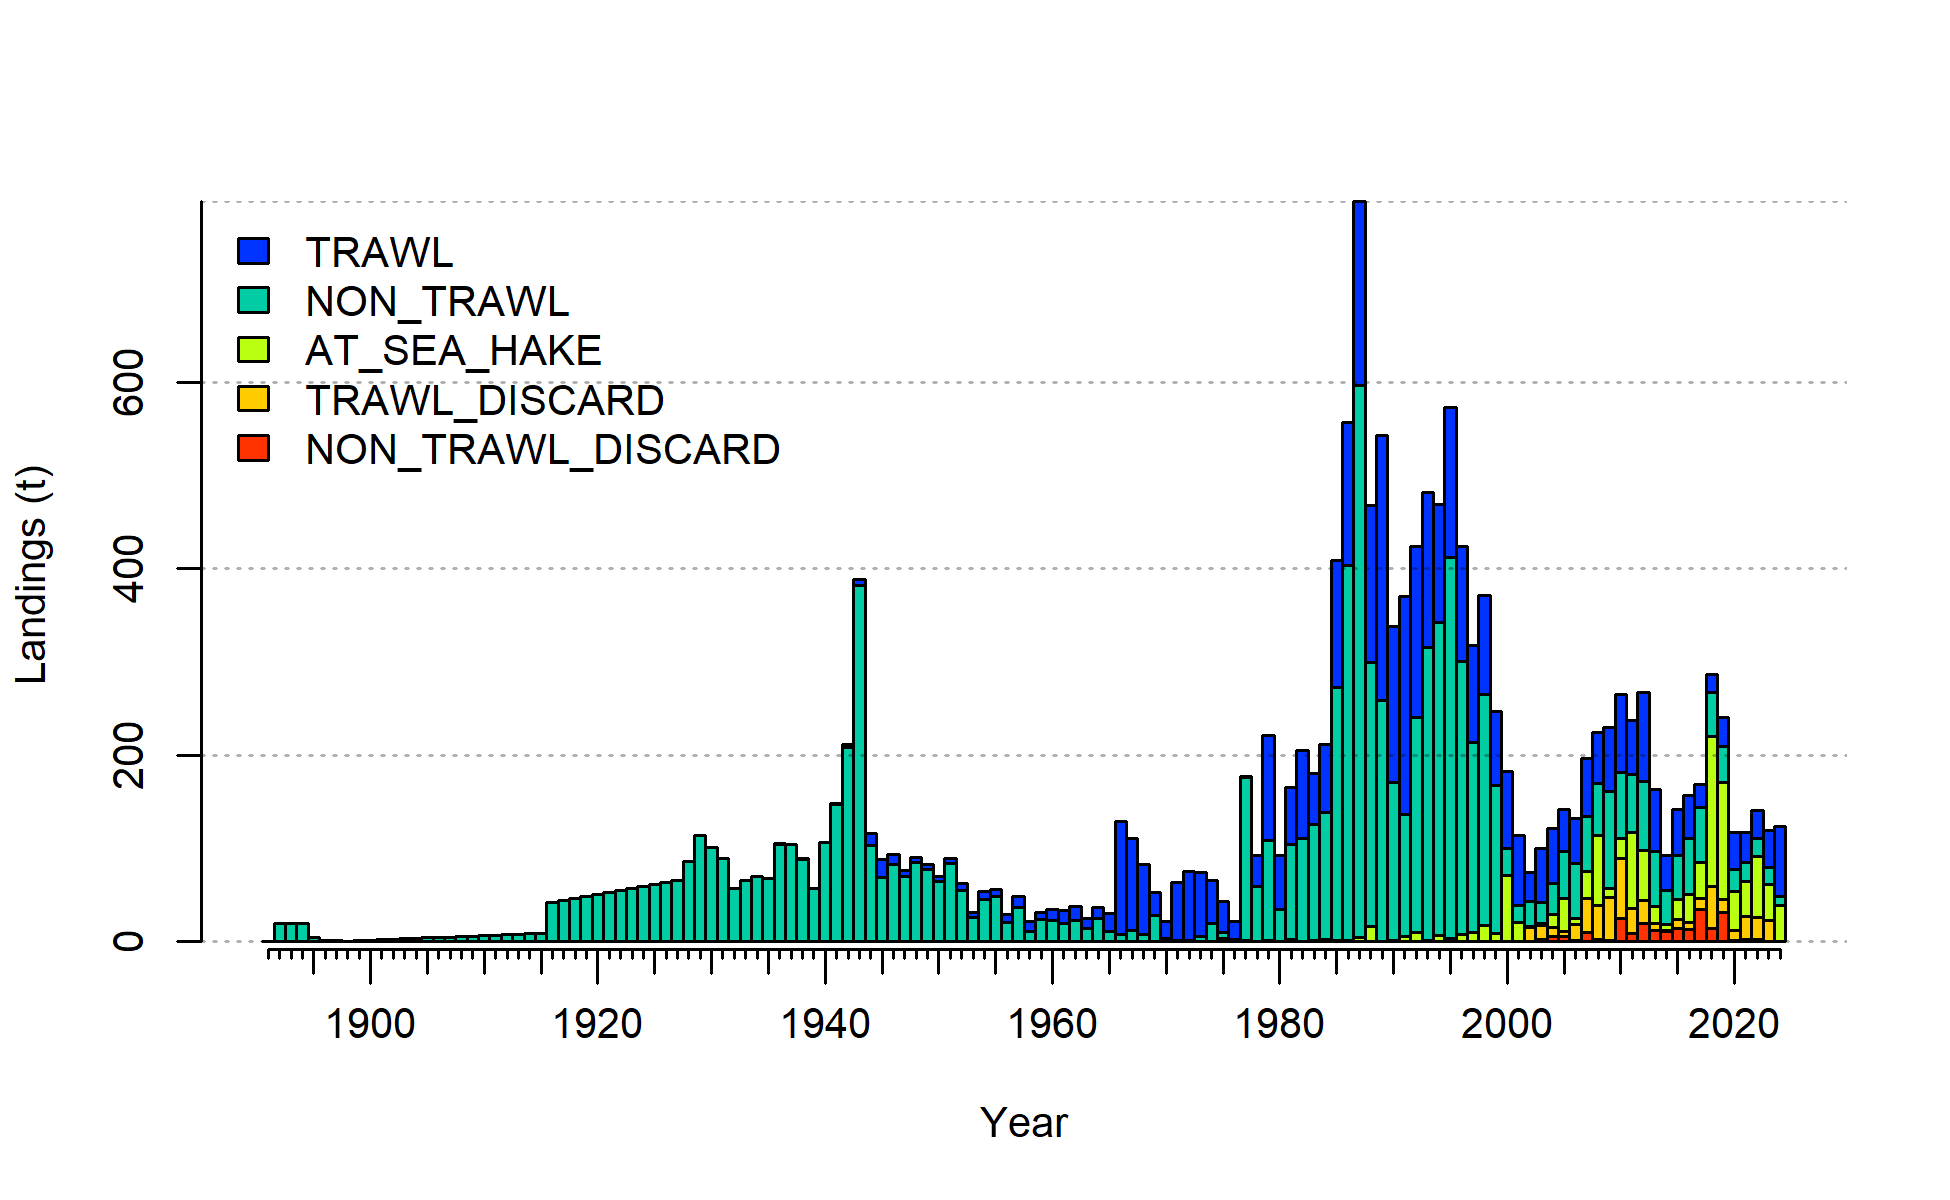
\includegraphics[keepaspectratio]{ref_model/plots/catch2_landings_stacked.png}}

}

\caption{\label{fig-es-landings}Landings in metric tons (mt) by year for
each fleet.}

\end{figure}%

\subsection{Data and Assessments}\label{data-and-assessments}

The only previous benchmark stock assessment for Rougheye/Blackspotted
Rockfishes for the U.S. West Coast area was done in 2013
(\citeproc{ref-hicks_status_2013}{Hicks, Wetzel, and Harms 2013}). It
was conducted with Stock Synthesis statistical catch-at-age modelling
framework (\citeproc{ref-MethotWetzel2013}{Methot and Wetzel 2013}).

This 2025 assessment also uses Stock Synthesis, version 3.30.23.1. The
modeling period begins in 1892, and the stock prior to that is assumed
to be in an unfished equilibrium condition.

Rougheye/Blackspotted Rockfishes fishery-dependent data in this
assessment are divided among six fleets, treating discard catches
separately from the retained fisheries. Following 2013 assessment, it
maintains the at-sea-hake fishery as its own fleet, and adds a mid-water
fishery that has emerged in the last decade. This stock assessment adds
10+ years of additional length data, and several more years of age data
(included as conditioned on length data). The same four surveys (the
West Coast Groundfish Bottom Trawl Survey (WCGBTS), AFSC/NWFSC Triennial
Shelf Survey, AFSC Slope Survey and NWFSC Slope Survey) as used in the
last stock assessment are used here, with an extension to 2024 to the
the WCGBTS. The index standardization of all survey data uses the newer
approach of applying spatiotemporal generalized linear mixed models.

This is a sex-specific model. Females and males have separate growth
curves and sex-specific weight-at-length parameters. Growth is assumed
to follow the von Bertalanffy growth model, and the assessment
explicitly estimates all parameters describing somatic growth. The
natural mortality for females is estimated in the assessment and natural
mortality for males is fixed an the value generated from meta-analytical
study. Externally estimated life history parameters, including those
defining the length-weight relationship, female fecundity and maturity
schedule were revised for this assessment to incorporate new
information. Recruitment dynamics are assumed to follow the
Beverton-Holt stock-recruit function, and recruitment deviations are
estimated. Stock-recruitment steepness is fixed at the value generated
from meta-analytical study. The base model estimates parameters for
selectivity based on length data, and estimated selectivity curves are a
mix of dome-shaped (for bottom trawl gears) and logistic (for mid-water
trawl).

\subsection{Stock Output and Dynamics}\label{stock-output-and-dynamics}

The model estimates that the stock complex currently is in a healthy
state, well above management target (Figure~\ref{fig-es-sb},
Figure~\ref{fig-es-depl}). Approximate confidence intervals based on the
asymptotic variance estimates show that the uncertainty in the estimated
spawning output is high. Estimates of spawning biomass in most recent
decade are shown in Table~\ref{tbl-es-sb}.

Fraction unfished shows slight decline between 1940s and the 1960s, also
also gradual decline since early-1980s, which correspond to catch
history.

\begingroup
\fontsize{9.0pt}{10.8pt}\selectfont

\begin{longtable}{>{\centering\arraybackslash}p{\dimexpr 56.25pt -2\tabcolsep-1.5\arrayrulewidth}>{\centering\arraybackslash}p{\dimexpr 56.25pt -2\tabcolsep-1.5\arrayrulewidth}>{\centering\arraybackslash}p{\dimexpr 56.25pt -2\tabcolsep-1.5\arrayrulewidth}>{\centering\arraybackslash}p{\dimexpr 56.25pt -2\tabcolsep-1.5\arrayrulewidth}>{\centering\arraybackslash}p{\dimexpr 56.25pt -2\tabcolsep-1.5\arrayrulewidth}>{\centering\arraybackslash}p{\dimexpr 56.25pt -2\tabcolsep-1.5\arrayrulewidth}>{\centering\arraybackslash}p{\dimexpr 56.25pt -2\tabcolsep-1.5\arrayrulewidth}}

\caption{\label{tbl-es-sb}Estimated recent trend in spawning output and
the fraction unfished and the 95 percent confidence intervals.}

\tabularnewline

\toprule
Year & Spawning output & Lower Interval (mt) & Upper Interval (mt) & Fraction Unfished & Lower Interval & Upper Interval \\ 
\midrule\addlinespace[2.5pt]
2015 & 4,980,900 & -2,394,288 & 12,356,088 & 0.882 & 0.648 & 1.115 \\ 
2016 & 4,969,060 & -2,407,049 & 12,345,169 & 0.880 & 0.644 & 1.116 \\ 
2017 & 4,954,890 & -2,421,278 & 12,331,058 & 0.877 & 0.638 & 1.116 \\ 
2018 & 4,940,000 & -2,435,893 & 12,315,893 & 0.875 & 0.633 & 1.116 \\ 
2019 & 4,914,900 & -2,461,287 & 12,291,087 & 0.870 & 0.623 & 1.117 \\ 
2020 & 4,893,960 & -2,484,403 & 12,272,323 & 0.867 & 0.615 & 1.118 \\ 
2021 & 4,891,660 & -2,492,289 & 12,275,609 & 0.866 & 0.613 & 1.119 \\ 
2022 & 4,895,290 & -2,498,792 & 12,289,372 & 0.867 & 0.613 & 1.121 \\ 
2023 & 4,900,660 & -2,508,945 & 12,310,265 & 0.868 & 0.612 & 1.123 \\ 
2024 & 4,913,840 & -2,516,952 & 12,344,632 & 0.870 & 0.614 & 1.126 \\ 
2025 & 4,929,140 & -2,527,955 & 12,386,235 & 0.873 & 0.615 & 1.130 \\ 
\bottomrule

\end{longtable}

\endgroup

\begin{figure}[H]

\centering{

\pandocbounded{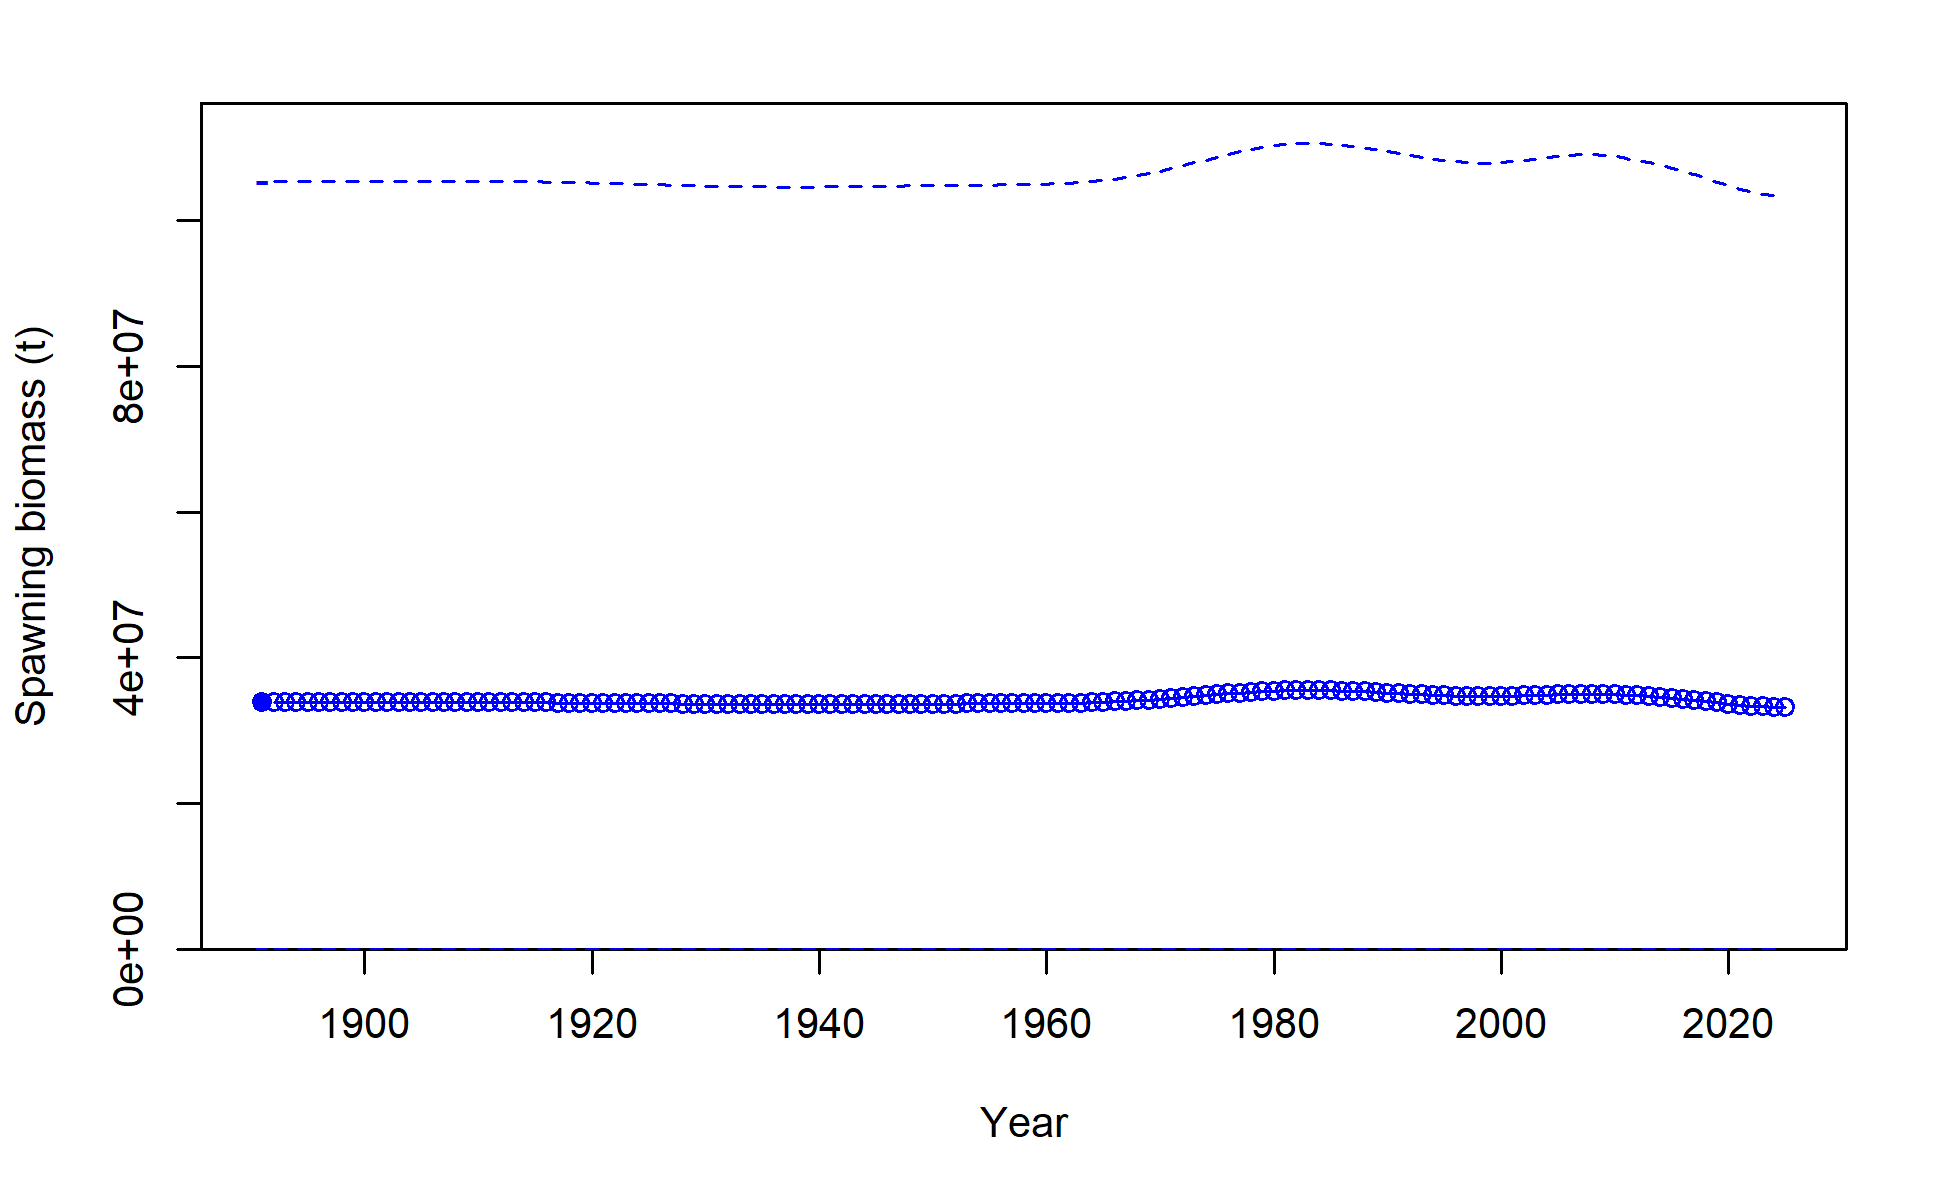
\includegraphics[keepaspectratio]{ref_model/plots/ts7_Spawning_output_with_95_intervals.png}}

}

\caption{\label{fig-es-sb}Estimated time series of spawning output
(trillions of eggs) for the base model.}

\end{figure}%

\begin{figure}[H]

\centering{

\pandocbounded{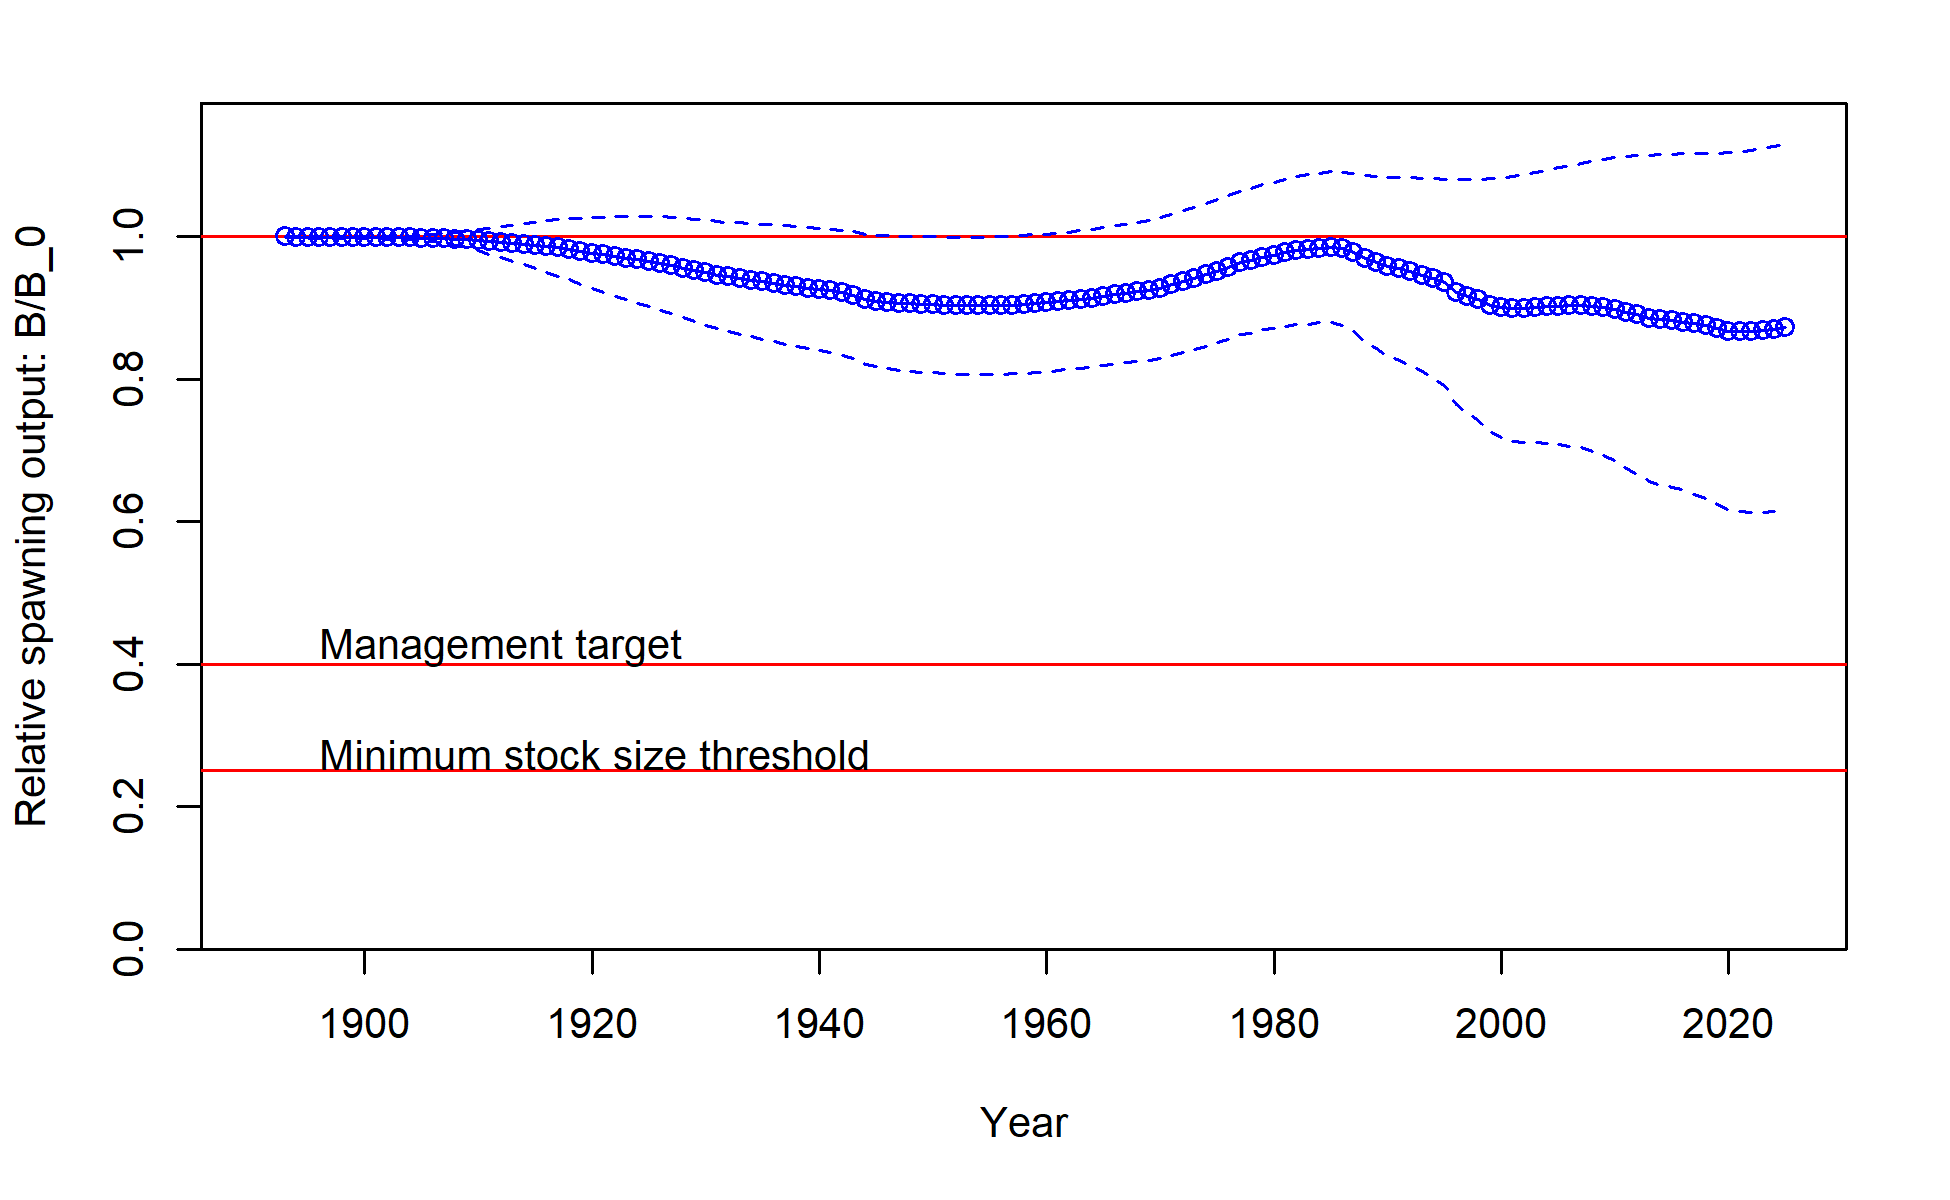
\includegraphics[keepaspectratio]{ref_model/plots/ts9_Relative_spawning_output_intervals.png}}

}

\caption{\label{fig-es-depl}Estimated time series of fraction of
unfished spawning output for the base model.}

\end{figure}%

\subsection{Recruitment}\label{recruitment}

Recruitment dynamics (Table~\ref{tbl-es-recr},
Figure~\ref{fig-es-recruits}) are assumed to follow Beverton-Holt
stock-recruit function and the steepness parameter was fixed at the
value of 0.72, which is the mean of steepness prior probability
distribution, derived from meta-analysis of rockfish stocks. The level
of virgin recruitment (R0) is estimated to inform the magnitude of the
initial stock size. Annual recruitment is treated as stochastic.
``Main'' recruitment deviations were estimated for modeled years between
1892 and 2023, with forecast recruitment period starting in 2024
(Figure~\ref{fig-es-recdevs}).

\clearpage

\begingroup
\fontsize{9.0pt}{10.8pt}\selectfont

\begin{longtable}{>{\centering\arraybackslash}p{\dimexpr 56.25pt -2\tabcolsep-1.5\arrayrulewidth}>{\centering\arraybackslash}p{\dimexpr 56.25pt -2\tabcolsep-1.5\arrayrulewidth}>{\centering\arraybackslash}p{\dimexpr 56.25pt -2\tabcolsep-1.5\arrayrulewidth}>{\centering\arraybackslash}p{\dimexpr 56.25pt -2\tabcolsep-1.5\arrayrulewidth}>{\centering\arraybackslash}p{\dimexpr 56.25pt -2\tabcolsep-1.5\arrayrulewidth}>{\centering\arraybackslash}p{\dimexpr 56.25pt -2\tabcolsep-1.5\arrayrulewidth}>{\centering\arraybackslash}p{\dimexpr 56.25pt -2\tabcolsep-1.5\arrayrulewidth}}

\caption{\label{tbl-es-recr}Estimated recent trend in recruitment
(1,000s) and recruitment deviations and the 95 percent confidence
intervals.}

\tabularnewline

\toprule
Year & Recruitment (1,000s) & Lower Interval (1,000s) & Upper Interval (1,000s) & Recruitment Deviations & Lower Interval & Upper Interval \\ 
\midrule\addlinespace[2.5pt]
2015 & 659 & 173 & 2,515 & -0.445 & -1.271 & 0.382 \\ 
2016 & 870 & 228 & 3,328 & -0.172 & -1.012 & 0.668 \\ 
2017 & 2,172 & 584 & 8,071 & 0.738 & -0.009 & 1.484 \\ 
2018 & 1,341 & 354 & 5,087 & 0.251 & -0.565 & 1.066 \\ 
2019 & 1,197 & 317 & 4,517 & 0.132 & -0.678 & 0.943 \\ 
2020 & 846 & 221 & 3,242 & -0.220 & -1.083 & 0.643 \\ 
2021 & 923 & 236 & 3,608 & -0.138 & -1.050 & 0.774 \\ 
2022 & 1,017 & 254 & 4,067 & -0.046 & -1.008 & 0.916 \\ 
2023 & 1,067 & 266 & 4,286 & -0.003 & -0.982 & 0.975 \\ 
2024 & 1,076 & 268 & 4,323 & 0.000 & -0.980 & 0.980 \\ 
2025 & 1,076 & 268 & 4,324 & 0.000 & -0.980 & 0.980 \\ 
\bottomrule

\end{longtable}

\endgroup

\begin{figure}[H]

\centering{

\pandocbounded{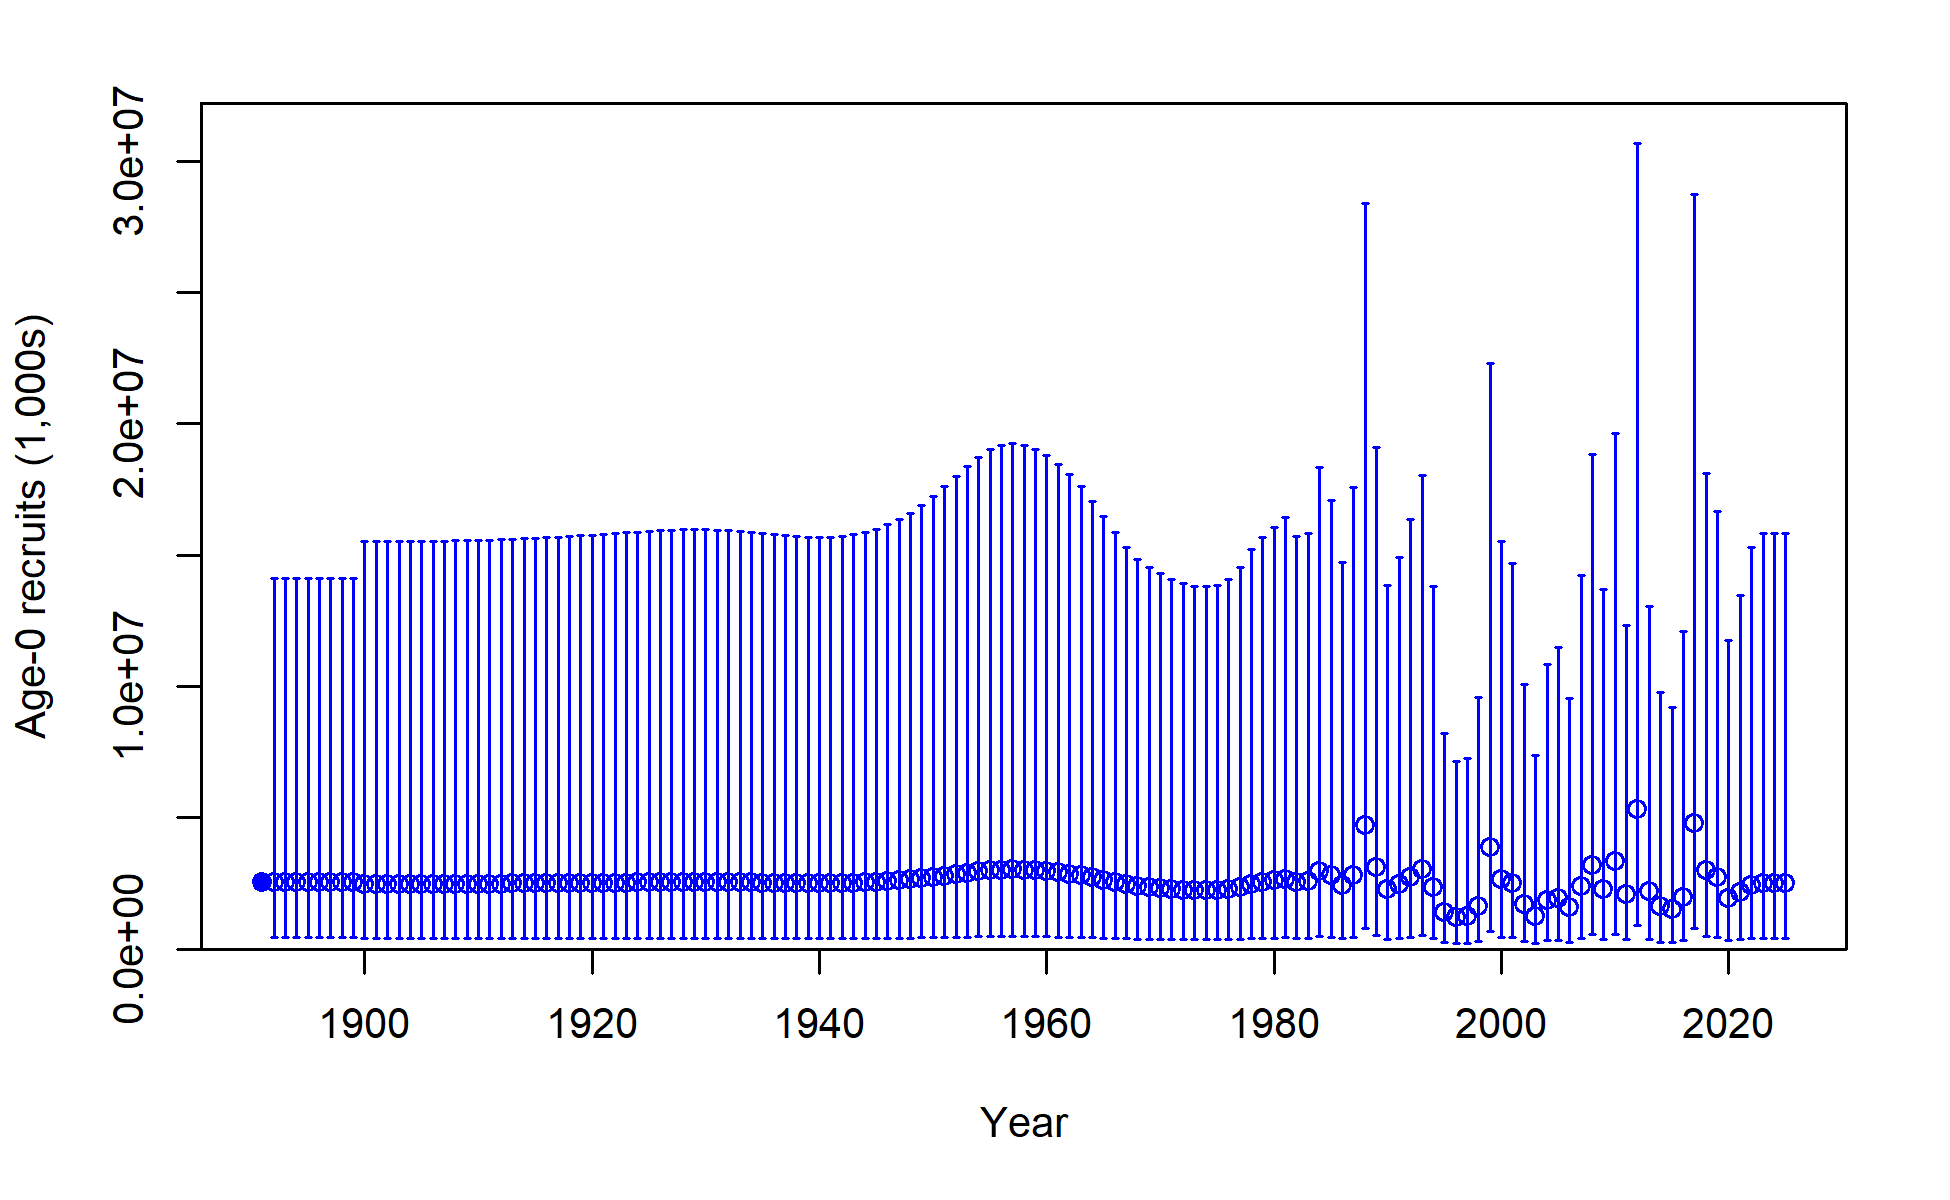
\includegraphics[keepaspectratio]{ref_model/plots/ts11_Age-0_recruits_(1000s)_with_95_asymptotic_intervals.png}}

}

\caption{\label{fig-es-recruits}Estimated time series of age-0 recruits
for the base model.}

\end{figure}%

\begin{figure}[H]

\centering{

\pandocbounded{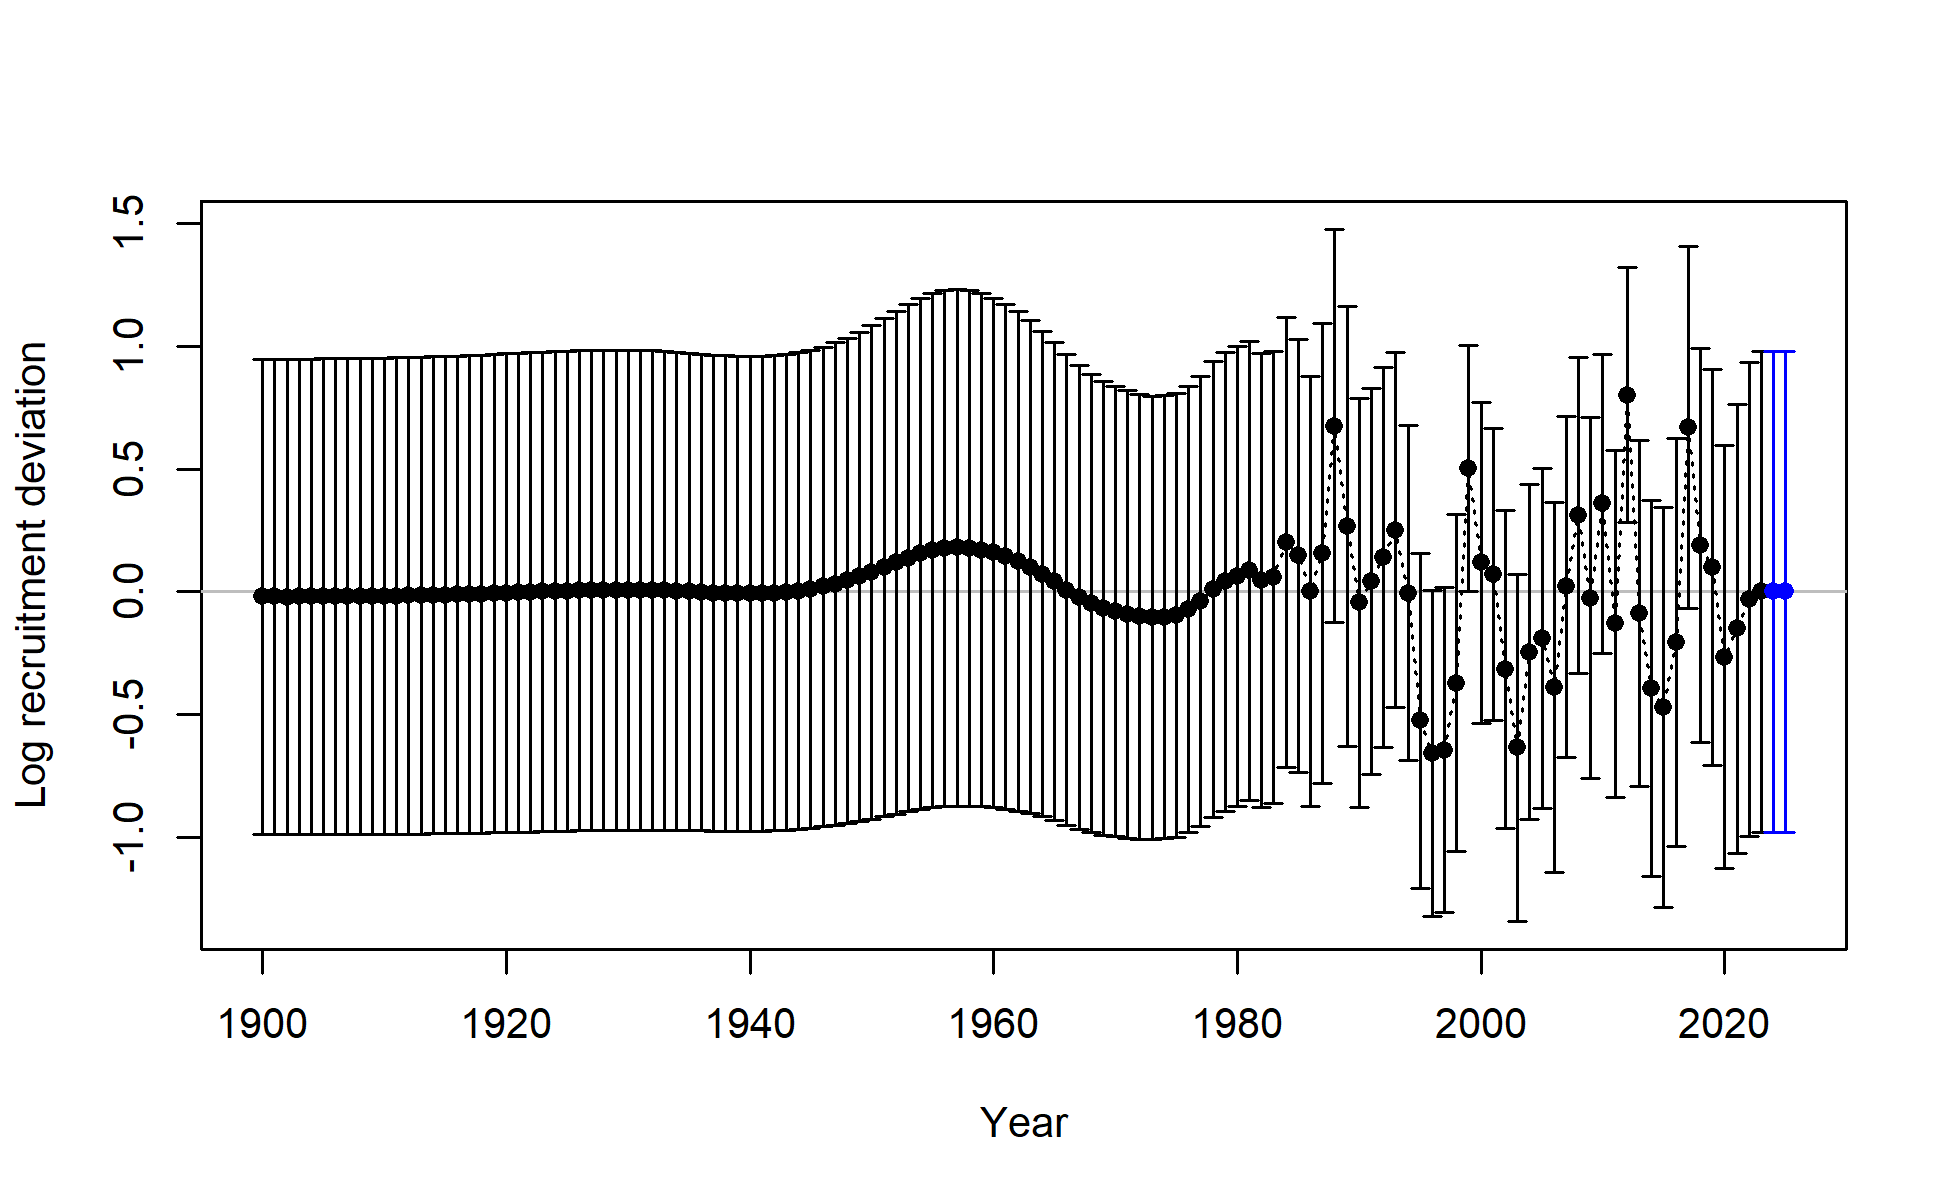
\includegraphics[keepaspectratio]{ref_model/plots/recdevs2_withbars.png}}

}

\caption{\label{fig-es-recdevs}Estimated time series of recruitment
deviations for the base model.}

\end{figure}%

\subsection{Exploitation Status}\label{exploitation-status}

Two measures of exploitation are fishing intensity and exploitation
rate. Fishing intensity is defined here as 1 - SPR, where SPR (Spawning
Potential Ratio) is the equilibrium spawning output at a given
combination of F and selectivity relative to spawning output at unfished
equilibrium. Using the units of 1-SPR means that more intense fishing is
associated with a higher value. The value of 1-SPR in the absence of
fishing is 0 and the maximum is 1.0 if all spawning fish are being
killed before spawning. The Pacific Fishery Management Council (PFMC)
has chosen an SPR target of 0.5 for Rougheye/Blackspotted Rockfishes so
harvest which leads to SPR below 0.5, or fishing intensity (1-SPR)
greater than 0.5 would be overfishing. Exploitation rate is defined as
the catch relative to age 26+ biomass. This metric is included because
interpretation is simple, but it is not used as a basis for management.

Exploitation rates were below the management target of a fishing
intensity that leads to a SPR of 0.5 throughout most of the time series
except for 1995, when the catch peaked at 744 metric tons
(Table~\ref{tbl-es-spr}, Figure~\ref{fig-es-spr}).

\begingroup
\fontsize{9.0pt}{10.8pt}\selectfont

\begin{longtable}{>{\centering\arraybackslash}p{\dimexpr 60.00pt -2\tabcolsep-1.5\arrayrulewidth}>{\centering\arraybackslash}p{\dimexpr 60.00pt -2\tabcolsep-1.5\arrayrulewidth}>{\centering\arraybackslash}p{\dimexpr 60.00pt -2\tabcolsep-1.5\arrayrulewidth}>{\centering\arraybackslash}p{\dimexpr 60.00pt -2\tabcolsep-1.5\arrayrulewidth}>{\centering\arraybackslash}p{\dimexpr 60.00pt -2\tabcolsep-1.5\arrayrulewidth}>{\centering\arraybackslash}p{\dimexpr 60.00pt -2\tabcolsep-1.5\arrayrulewidth}>{\centering\arraybackslash}p{\dimexpr 60.00pt -2\tabcolsep-1.5\arrayrulewidth}}

\caption{\label{tbl-es-spr}Estimated recent trend in fishing intensity
1-SPR, where SPR is the spawning potential ratio, and the exploitation
rate, along with the 95 percent confidence intervals for both
quantities.}

\tabularnewline

\toprule
Year & 1-SPR & Lower Interval (SPR) & Upper Interval (SPR) & Exploitation Rate & Lower Interval (Rate) & Upper Interval (Rate) \\ 
\midrule\addlinespace[2.5pt]
2015 & 0.114 & -0.038 & 0.266 & 0.004 & -0.002 & 0.011 \\ 
2016 & 0.127 & -0.041 & 0.296 & 0.005 & -0.002 & 0.013 \\ 
2017 & 0.133 & -0.042 & 0.307 & 0.005 & -0.003 & 0.013 \\ 
2018 & 0.188 & -0.047 & 0.423 & 0.008 & -0.004 & 0.021 \\ 
2019 & 0.180 & -0.048 & 0.408 & 0.008 & -0.004 & 0.019 \\ 
2020 & 0.090 & -0.034 & 0.213 & 0.004 & -0.002 & 0.009 \\ 
2021 & 0.079 & -0.031 & 0.190 & 0.003 & -0.002 & 0.008 \\ 
2022 & 0.098 & -0.036 & 0.233 & 0.004 & -0.002 & 0.010 \\ 
2023 & 0.083 & -0.032 & 0.199 & 0.003 & -0.002 & 0.009 \\ 
2024 & 0.098 & -0.036 & 0.233 & 0.004 & -0.002 & 0.011 \\ 
\bottomrule

\end{longtable}

\endgroup

\begin{figure}[H]

\centering{

\pandocbounded{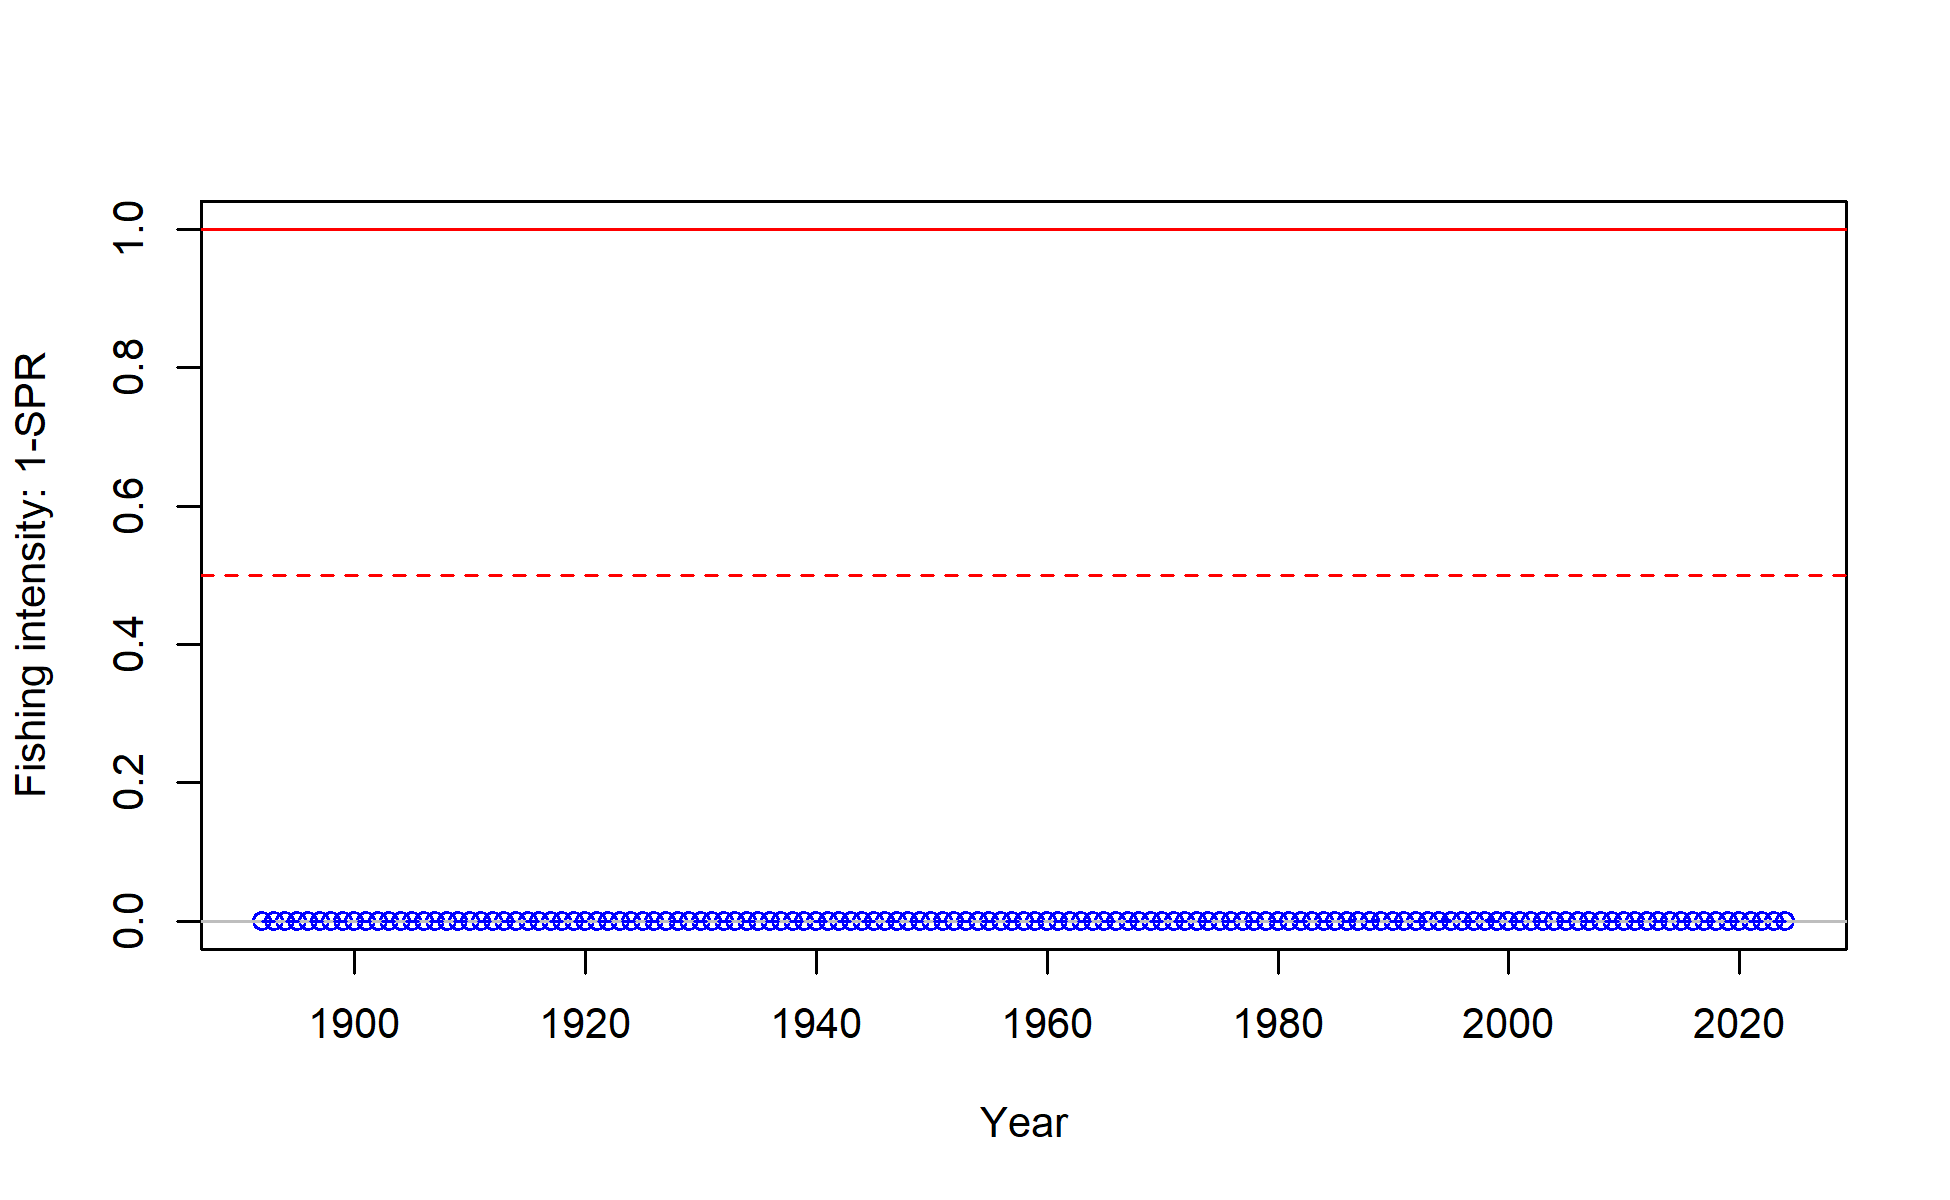
\includegraphics[keepaspectratio]{ref_model/plots/SPR3_ratiointerval.png}}

}

\caption{\label{fig-es-spr}Estimated time series of the fishing
intensity (1 - SPR), where SPR is the spawning potential ratio, with
approximate 95\% asymptotic intervals. The horizontal line at 0.5
corresponds to SPR = 0.5, the management reference point. The horizontal
line at 1.0 corresponds to SPR = 0 (all spawning fish removed from the
population).}

\end{figure}%

\subsection{Ecosysystem Consideration}\label{ecosysystem-consideration}

Rockfishes are an important component of the California Current
ecosystem along the U.S. West Coast, with its many dozens of species
filling various niches in both soft and hard bottom habitats from the
nearshore to the continental slope. Rougheye/Blackspotted Rockfishes are
one of the larger species of rockfishes and occupy shelf areas when they
are young and move into deeper slope waters with age. As they age, they
tend to become more solitary, but may form aggregations during the
spawning season. Due to a paucity of life-history data for
Rougheye/Blackspotted Rockfishes, most ecosystem considerations are
implied from the understanding of rockfishes in general.

Recruitment is one mechanism by which the ecosystem may directly impact
the population dynamics of Rougheye/Blackspotted Rockfishes. The
specific pathways through which environmental conditions exert influence
on Rougheye/Blackspotted Rockfishes dynamics are unclear, however,
changes in water temperature and currents, distribution of prey and
predators, and the amount and timing of upwelling are all possible
linkages. Changes in the environment may also result in changes in
age-at-maturity, fecundity, growth, and survival which can affect how
the status of the stock and its susceptibility to fishing are
determined. Unfortunately, there are no data for Rougheye/Blackspotted
Rockfishes that provide insights into these effects.

\subsection{Reference Points}\label{reference-points}

Estimates of the current state of the population, as well as reference
points based on 1) a target unfished spawning output of 40\%, 2) a
spawning potential ratio of 0.5, and 3) the model estimate of maximum
sustainable yield, are all listed in Table~\ref{tbl-ref-points-es}.
Equilibrium yield curve for the base case model is shown in
Figure~\ref{fig-es-yield}.

Unfished spawning stock output for Rougheye/Blackspotted Rockfishes is
estimated to be 5,647,660 million eggs (95\% confidence interval:
,\textless1--12,581,189 million eggs). The management biomass target for
Rougheye/Blackspotted Rockfishes is defined as 40\% of the unfished
spawning output (𝐵40\%), which is estimated by the model to be 2,259,070
million eggs (95\% confidence interval: \textless1--5,032,478 million
eggs), which corresponds, in a theoretical equilibrium state, to an
exploitation rate (catch / age 26+ biomass) of 0.048
(Table~\ref{tbl-ref-points-es}, Figure~\ref{fig-es-yield}). This harvest
rate provides an equilibrium yield of 553 mt at 𝐵40\% (95\% confidence
interval: 0--1,224 mt). Catch limits are determined by an SPR = 50\%
reference point which is associated with equilibrium exploitation rate
of 0.040. The model estimate of maximum sustainable yield (MSY) is 592
mt (95\% confidence interval: 0--1,311 mt). The estimated spawning stock
output at MSY is 1,497,160 million eggs (95\% confidence interval:
0--3,337,633 million eggs). The exploitation rate corresponding to the
estimated FMSY proxy of SPR = 34\% is 0.085.

\clearpage

\begingroup
\fontsize{9.0pt}{10.8pt}\selectfont

\begin{longtable}{lrrr}

\caption{\label{tbl-ref-points-es}Summary of reference points and
management quantities, including estimates of the 95 percent confidence
intervals. SO is spawning output, SPR is the spawning potential ratio,
and MSY is maximum sustainable yield.}

\tabularnewline

\toprule
Reference Point & Estimate & Lower Interval & Upper Interval \\ 
\midrule\addlinespace[2.5pt]
Unfished Spawning output & 5,647,680.0 & -1,285,908.2 & 12,581,268.2 \\ 
Unfished Age 26+ Biomass (mt) & 33,631 & -7,664 & 74,925 \\ 
Unfished Recruitment (R0) & 1,092 & -237 & 2,420 \\ 
2025 Spawning output & 4,929,140 & -2,527,955 & 12,386,235 \\ 
2025 Fraction Unfished & 0.873 & 0.615 & 1.130 \\ 
Reference Points Based SO40\% & — & — & — \\ 
Proxy Spawning output SO40\% & 2,259,070 & -514,357 & 5,032,497 \\ 
SPR Resulting in SO40\% & 0.458 & 0.458 & 0.458 \\ 
Exploitation Rate Resulting in SO40\% & 0.048 & 0.045 & 0.051 \\ 
Yield with SPR Based On SO40\% (mt) & 553 & -119 & 1,224 \\ 
Reference Points Based on SPR Proxy for MSY & — & — & — \\ 
Proxy Spawning output (SPR50) & 2,519,730 & -573,720 & 5,613,180 \\ 
SPR50 & 0.500 & — & — \\ 
Exploitation Rate Corresponding to SPR50 & 0.040 & 0.038 & 0.042 \\ 
Yield with SPR50 at SO SPR (mt) & 526 & -113 & 1,165 \\ 
Reference Points Based on Estimated MSY Values & — & — & — \\ 
Spawning output at MSY (SO MSY) & 1,497,170 & -343,318 & 3,337,658 \\ 
SPR MSY & 0.337 & 0.334 & 0.339 \\ 
Exploitation Rate Corresponding to SPR MSY & 0.085 & 0.079 & 0.090 \\ 
MSY (mt) & 592 & -127 & 1,311 \\ 
\bottomrule

\end{longtable}

\endgroup

\begin{figure}[H]

\centering{

\pandocbounded{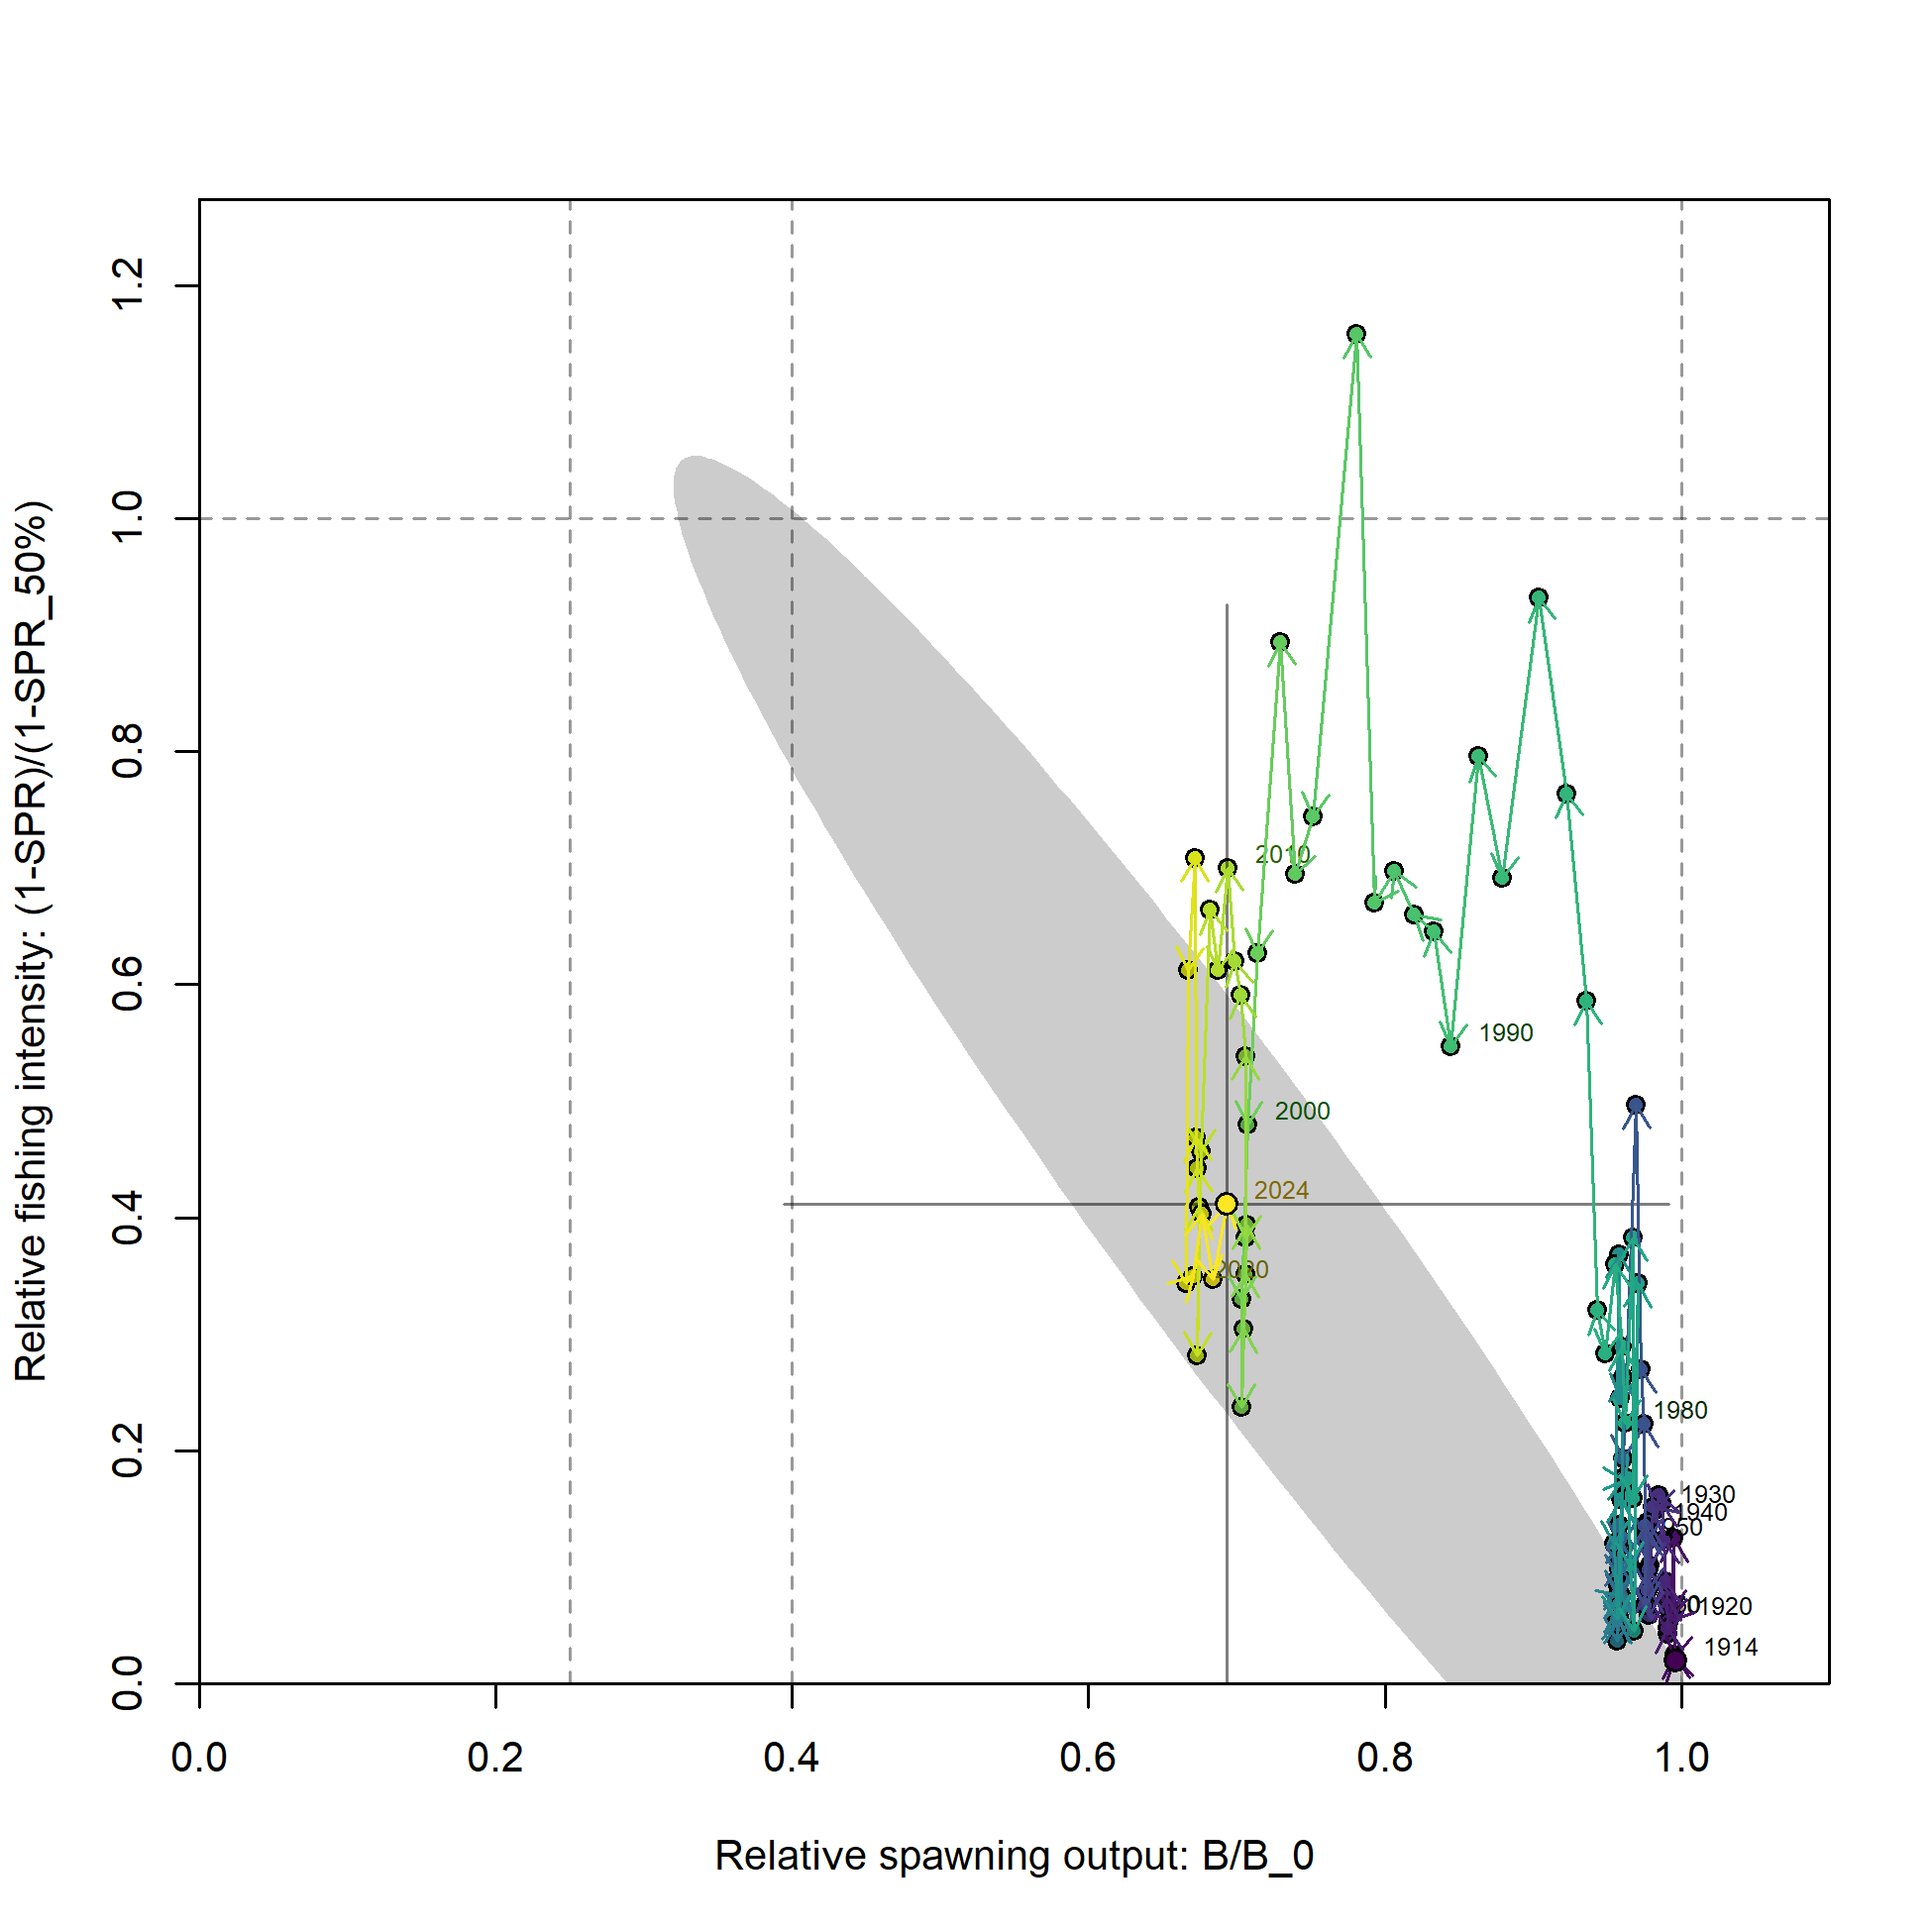
\includegraphics[keepaspectratio]{ref_model/plots/SPR4_phase.png}}

}

\caption{\label{fig-es-kobe}Phase plot of fishing intensity versus
fraction unfished.}

\end{figure}%

\begin{figure}[H]

\centering{

\pandocbounded{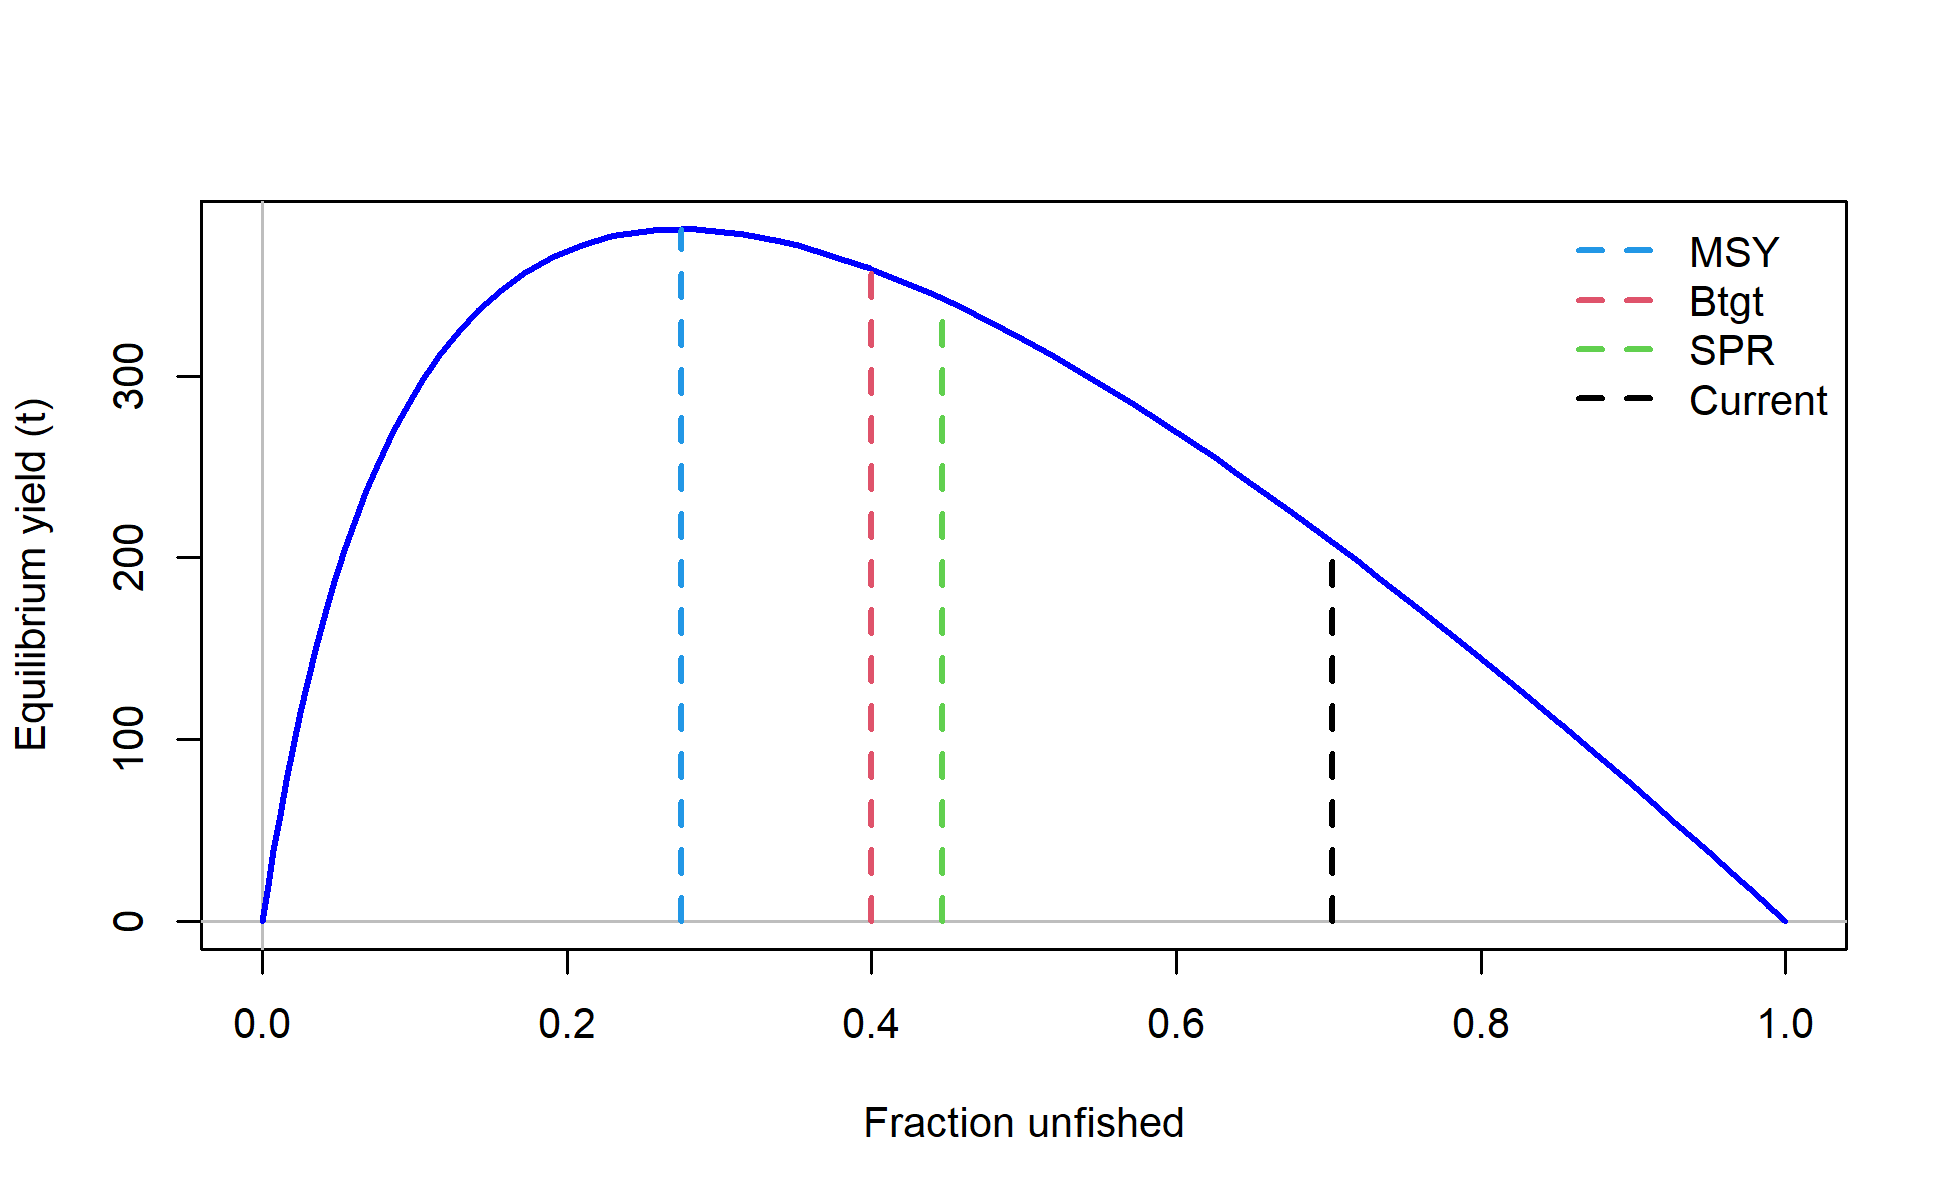
\includegraphics[keepaspectratio]{ref_model/plots/yield2_yield_curve_with_refpoints.png}}

}

\caption{\label{fig-es-yield}Equilibrium yield curve for the base case
model. Values are based on the most recent fishery selectivities and
retention curves and with steepness fixed at 0.72.}

\end{figure}%

\subsection{Management Performance}\label{management-performance}

In the last ten years total dead catches of Rougheye/Blackspotted
Rockfishes have been below the annual catch limit. The last ten years
total dead catches for Rougheye/Blackspotted Rockfishes against the
overfishing limits (OFLs), the acceptable biological catches (ABCs), the
annual catch limits (ACLs) are shown in Table~\ref{tbl-es-management}.

\begingroup
\fontsize{9.0pt}{10.8pt}\selectfont

\begin{longtable}{rrrrr}

\caption{\label{tbl-es-management}Recent trend in the overfishing limits
(OFL), the acceptable biological catches (ABCs), the annual catch limits
(ACLs), and the total dead catch (landings + discards) all in metric
tons (mt). Specifications are combined across north and south of 40'10.}

\tabularnewline

\toprule
Year & OFL (mt) & ABC (mt) & ACL (mt) & Catch (mt) \\ 
\midrule\addlinespace[2.5pt]
2015 & 206 & 188.1 & 188.1 & 132.1 \\ 
2016 & 211 & 192.7 & 192.7 & 149.0 \\ 
2017 & 215 & 196.3 & 196.3 & 156.0 \\ 
2018 & 219 & 199.9 & 199.9 & 241.5 \\ 
2019 & 222 & 202.7 & 202.7 & 226.6 \\ 
2020 & 224 & 204.5 & 204.5 & 106.1 \\ 
2021 & 237 & 195.8 & 195.8 & 92.8 \\ 
2022 & 238 & 194.7 & 194.7 & 117.4 \\ 
2023 & 238 & 192.8 & 192.8 & 97.6 \\ 
2024 & 238 & 194.7 & 194.7 & 118.9 \\ 
\bottomrule

\end{longtable}

\endgroup

\subsection{Unresolved problems and major
uncertainties}\label{unresolved-problems-and-major-uncertainties}

Rougheye/Blackspotted Rockfishes is relatively lightly exploited stock.
The maximum catch amount of 744 metric tons was observed in 1995, and
the average removals over the entire time period of exploitation is
slightly over 100 metric tons. For comparison, Widow Rockfish catches
for in the recent years were reaching over 12,000 metric tons, and in
the early 1980s they were exceeding 28,000 metric tons. Most likely,
catches of Rougheye/Blackspotted Rockfishes were not substantial because
the complex is associated with steep slopes and boulder habitats,
difficult to access with bottom trawl gears. Plus, it primarily occurs
in the northern part of the assessed area (off Oregon and Washington),
and is only rarely taken by fisheries in California. Given this
relatively light exploitation, the scale of Rougheye/Blackspotted
Rockfishes stock is uncertain, as we did not observe large contrasts in
the stock dynamics. Such contrasts (``two-way trips'') provide more
reliable information about carrying capacity, the intrinsic growth rate
as well as scale of the population.

Through extensive explorations, we found that stock scale is sensitive
to assumptions about shape of the selectivity curves, especially for the
bottom trawl and non-trawl fleet. In the previous assessment all fleets
(except for Triennial Survey) were assumed asymptotic. In this
assessment, we provide flexibility for the bottom trawl fleet and bottom
trawl surveys to estimate dome-shaped selectivity curves. Changes in
selectivity assumptions allow to substantially improve fits to length
and age composition data in fisheries and surveys, but also resulted in
a substantial increase of stock scale.

Stock scale is also sensitive to assumptions about natural mortality.
Rougheye/Blackspotted Rockfishes are one of the longest lived species of
rockfish on the West Coast, with maximum ages of 169 years in this
assessment. Individual as old as 205 years are reported in literature.
It is, therefore, likely that natural mortality for
Rougheye/Blackspotted Rockfishes is lower than for other rockfish
species. With length and age data available only for years after 1994,
there is limited ability to monitor the long-term changes of aging
cohorts. Therefore, estimates of natural mortality are uncertain. This
assessment attempts to capture uncertainty in this parameter and
integrate it into the derived biomass estimates by estimating natural
mortality for females, while fixing the male natural mortality at the
value from meta-analytical study.

\subsection{Scientific Uncertainty}\label{scientific-uncertainty}

The model estimated uncertainty (\(\sigma\)) around the 2025 spawning
output for is 0.6836465. The uncertainty around the OFL is 0.6713586.
These values underestimate the overall uncertainty as they do not
incorporate the model structural uncertainty and do not account for any
time-varying dynamics other than recruitment. The estimated uncertainty
values are higher than the Category 1 default of 0.5, so all projections
will use the estimated (\(\sigma\)).

\subsection{Harvest Projections and Decision
Tables}\label{harvest-projections-and-decision-tables}

Projections of the overfishing limit, acceptable biological catch, and
annual catch limit, all based on a \(P^*\) of 0.45 and a log-space
standard deviation of the overfishing limit (\(\sigma\)) of 0.68 (as
estimated in this model) are included in Table~\ref{tbl-es-projections}.
Assumed catches for 2025 and 2026 for this projection were provided by
the PFMC Groundfish Management Team, and catches from 2027 onward assume
full attainment of the acceptable biological catch.

No decision table needed in draft assessments undergoing review.

\begin{landscape}
\begingroup
\fontsize{9.0pt}{10.8pt}\selectfont

\begin{longtable}{>{\centering\arraybackslash}p{\dimexpr 56.25pt -2\tabcolsep-1.5\arrayrulewidth}>{\centering\arraybackslash}p{\dimexpr 56.25pt -2\tabcolsep-1.5\arrayrulewidth}>{\centering\arraybackslash}p{\dimexpr 56.25pt -2\tabcolsep-1.5\arrayrulewidth}>{\centering\arraybackslash}p{\dimexpr 56.25pt -2\tabcolsep-1.5\arrayrulewidth}>{\centering\arraybackslash}p{\dimexpr 56.25pt -2\tabcolsep-1.5\arrayrulewidth}>{\centering\arraybackslash}p{\dimexpr 56.25pt -2\tabcolsep-1.5\arrayrulewidth}>{\centering\arraybackslash}p{\dimexpr 56.25pt -2\tabcolsep-1.5\arrayrulewidth}>{\centering\arraybackslash}p{\dimexpr 56.25pt -2\tabcolsep-1.5\arrayrulewidth}>{\centering\arraybackslash}p{\dimexpr 56.25pt -2\tabcolsep-1.5\arrayrulewidth}>{\centering\arraybackslash}p{\dimexpr 56.25pt -2\tabcolsep-1.5\arrayrulewidth}}

\caption{\label{tbl-es-projections}Potential OFLs (mt), ABCs (mt), ACLs
(mt), the buffer between the OFL and ABC, estimated spawning output, and
fraction unfished with adopted OFLs and ACLs and assumed catch for the
first two years of the projection period.}

\tabularnewline

\toprule
Year & Adopted OFL (mt) & Adopted ACL (mt) & Assumed Catch (mt) & OFL (mt) & Buffer & ABC (mt) & ACL (mt) & Spawning output & Fraction Unfished \\ 
\midrule\addlinespace[2.5pt]
2025 & — & — & 141 & — & — & — & — & 4,929,140.000 & 0.873 \\ 
2026 & — & — & 174 & — & — & — & — & 4,945,630.000 & 0.876 \\ 
2027 & — & — & — & 980 & 0.913 & 894 & 894 & 4,960,900.000 & 0.878 \\ 
2028 & — & — & — & 968 & 0.908 & 878 & 878 & 4,888,090.000 & 0.866 \\ 
2029 & — & — & — & 955 & 0.902 & 862 & 862 & 4,818,790.000 & 0.853 \\ 
2030 & — & — & — & 944 & 0.896 & 846 & 846 & 4,752,560.000 & 0.842 \\ 
2031 & — & — & — & 932 & 0.890 & 830 & 830 & 4,688,990.000 & 0.830 \\ 
2032 & — & — & — & 921 & 0.885 & 815 & 815 & 4,627,620.000 & 0.819 \\ 
2033 & — & — & — & 909 & 0.879 & 799 & 799 & 4,567,870.000 & 0.809 \\ 
2034 & — & — & — & 898 & 0.874 & 784 & 784 & 4,509,380.000 & 0.798 \\ 
2035 & — & — & — & 886 & 0.868 & 769 & 769 & 4,451,710.000 & 0.788 \\ 
2036 & — & — & — & 874 & 0.863 & 755 & 755 & 4,394,830.000 & 0.778 \\ 
\bottomrule

\end{longtable}

\endgroup

\end{landscape}

\subsection{Research and Data Needs}\label{research-and-data-needs}

There are many areas of research that would benefit the understanding
and assessment of Rougheye/Blackspotted Rockfishes. Below, we identify
several of them that we consider particularly important.

\begin{itemize}
\item
  Understanding the stock structure and biology of Rougheye and
  Blackspotted Rockfishes: This assessment reports the status of
  Rougheye/Blackspotted Rockfishes as a pooled complex because it is
  extremely difficult to separate the catches of each species even in
  recent data, and attempting to do so would greatly increase the
  uncertainty in the predictions. Because little is known about the
  respective biology and catch histories of the two species, it is
  unclear whether managing them as a complex may place one species at
  disproportionate risk of overfishing relative to the other. Additional
  research that will provide insight into the distribution, life
  history, biological characteristics, and catch and discard profiles of
  the two species is recommended. Such an endeavor would like require
  the efforts of at sea observers in all fleets, biologists aboard
  fishery-independent surveys, and port samplers along the entire West
  Coast requiring broad, inter-agency collaboration.
\item
  Understanding of coatwide stock structure, connectivity, and
  distribution: This is a stock assessment for Rougheye/Blackspotted
  Rockfishes off of the west coast of the U.S. and does not consider
  data from British Columbia or Alaska. Further investigating and
  comparing the data and predictions from British Columbia and Alaska to
  determine if there are similarities with the U.S. West Coast
  observations would help to define the connectivity between rougheye
  rockfish north of the U.S.-Canada border.
\item
  Natural mortality: Uncertainty in natural mortality translates into
  uncertain estimates of status and sustainable fishing levels for
  Rougheye/Blackspotted Rockfishes. Assessment model was able to
  estimate female natural mortality, consistent with maximum age based
  meta-analytical prior, but male natural mortality was fixed in the
  model. The collection of additional age data and further research of
  the life-history of Rougheye/Blackspotted Rockfishes may improve our
  understanding of Rougheye/Blackspotted Rockfishes natural mortality.
\item
  Historical landings and discards, including investigation of fisheries
  selectivity: The substantial progress has been made in reconstructing
  historical landings of rockfishes on the U.S. West Coast, including
  those for Rougheye/Blackspotted Rockfishes. This assessment
  highlighted the importance of understanding of fishery selectivity
  assumptions associated with removals and how fishery selectivity
  changes throughout the years. Further understanding of this area would
  help reduce uncertainty in estimated scale of the stock.
\end{itemize}

\newpage{}

\setlength{\parskip}{5mm plus1mm minus1mm}
\pagenumbering{arabic}
\setcounter{page}{1}
\setcounter{section}{0}
\renewcommand{\thefigure}{\arabic{figure}}
\setcounter{figure}{0}
\renewcommand{\thetable}{\arabic{table}}
\setcounter{table}{0}

\section{Introduction}\label{introduction}

Rougheye (\emph{Sebastes aleutianus}) and Blackspotted (\emph{Sebastes
melanostictus}) rockfishes are two species that form one management
complex.

Rougheye rockfish are a long-lived rockfish named after a series of 2-10
spines along the lower rim of their eyes. They have also been called
blackthroat or blacktip rockfish
(\citeproc{ref-love_rockfishes_2002}{Love, Yoklavich, and Thorsteinson
2002}; \citeproc{ref-love_certainly_2011}{Love 2011}). Blackspotted
rockfish are distributed in similar locations as rougheye rockfish and
it is very difficult to visually distinguish the two species. These two
species may hybridize on occasion
(\citeproc{ref-love_certainly_2011}{Love 2011}).

It has only been from recent genetic studies that these two separate
species have been identified
(\citeproc{ref-gharrett_genetically_2006}{A. J. Gharrett et al. 2006};
\citeproc{ref-hawkins_genetic_2005}{S. L. Hawkins et al. 2005}) and have
had phenotypic characteristics useful for identifying the species in the
field identified (\citeproc{ref-gharrett_genetically_2006}{A. J.
Gharrett et al. 2006}; \citeproc{ref-orr_species_2008}{Orr and Hawkins
2008}). Before then, data are available for one species called Rougheye
Rockfish which included Rougheye Rockfish and Blackspotted Rockfish. Due
to the difficulty in distinguishing these two species and the lack of
historical separation of the species in all of the data, this assessment
combines any data for Blackspotted Rockfish with Rougheye Rockfish into
Rougheye/Blackspotted Rockfishes and provides management advice for the
two species combined. These species are also closely related to
Shortraker Rockfish (\emph{Sebastes borealis}) and are sometimes
difficult to distinguish from Shortraker Rockfish without looking at the
gill rakers.

\subsection{Stock Structure}\label{sec-stock_structure}

There are at least two questions to think about when considering stock
structure for Rougheye/Blackspotted Rockfishes when doing a stock
assessment.

\begin{itemize}
\tightlist
\item
  Since Rougheye and Blackspotted Rockfishes are two different species,
  can they be separated as two stocks and conduct separate assessments?
\end{itemize}

Rougheye rockfish were first described in 1811 as \emph{Perca
variabilis} by German zoologist Peter Simon Pallas
(\citeproc{ref-jordan_fishes_1898}{Jordan and Evermann 1898}), and
assigned to various taxa at least 15 times since
(\citeproc{ref-love_rockfishes_2002}{Love, Yoklavich, and Thorsteinson
2002}). Some descriptions noted both light and dark color morphs, which,
along with possible confusion with several morphologically similar
co-occurring species (e.g., \emph{Sebastes borealis} and \emph{Sebastes
melanostomus}) have contributed to the persistent ambiguity in formal
descriptions of Rougheye Rockfish (\citeproc{ref-orr_species_2008}{Orr
and Hawkins 2008}). The first genetic studies conducted in the late
1960s and early 1970s (\citeproc{ref-tsuyuki_contribution_1968}{Tsuyuki
et al. 1968}; \citeproc{ref-tsuyuki_analyses_1970}{Tsuyuki and Westrheim
1970}) observed diversity suggestive of two genetic types within
specimens identified as Rougheye Rockfish. Allozyme studies conducted
over the next two decades (\citeproc{ref-seeb_biochemical_1986}{Seeb
1986}; \citeproc{ref-hawkins_genetic_1997}{S. Hawkins, Heifetz, and Pohl
1997}; \citeproc{ref-hawkins_genetic_2005}{S. L. Hawkins et al. 2005})
provided additional evidence suggesting two separate genetic types
within field-identified Rougheye Rockfish. Genetic variation between the
two types, supported by both nuclear and mitochondrial DNA, was
determined to be sufficiently conclusive to separate two species: ``Type
I'' and ``Type II'' Rougheye Rockfish
(\citeproc{ref-gharrett_two_2005}{Anthony J. Gharrett et al. 2005}).
Meristic and morphometric comparisons of the two species suggested
certain characters, such as gill raker counts and length, snout length,
anal base length, and pectoral fin base, were significantly different,
and in combination could reliably, though not definitively, distinguish
between the species (\citeproc{ref-gharrett_genetically_2006}{A. J.
Gharrett et al. 2006}). The two separate species were formally
re-described by Orr and Hawkins (\citeproc{ref-orr_species_2008}{2008})
with the Type II group retaining \emph{Sebastes aleutianus} and the
common name Rougheye Rockfish. Blackspotted Rockfish was proposed as the
common name for the Type I group along with the scientific name of
\emph{Sebastes melanostictus}, re-establishing nomenclature from one of
the species complex's earlier descriptions
(\citeproc{ref-matsubara_1934}{Matsubara 1934}).

These two species remain difficult to consistently differentiate
visually in the catch, thus are still commonly reported and treated as a
species complex. Otolith morphometrics (e.g., shape, size, weight) have
shown some promise in possibly identifying these species in Alaskan
waters (97.3\% Blackspotted and 86.2\% of Rougheye rockfishes were
accurately identified) and possibly using older otoliths to break out
historical information by species
(\citeproc{ref-harris_using_2019}{Harris, Hutchinson, and Wildes 2019}).
Frey et al.~(in prep.) provided insight into the ability of the
Northwest Fisheries Science Center West Coast Groundfish Bottom Trawl
Survey biologists to identify the two species, with 90\% of genetically
identified Rougheye rockfish being correctly identified in the field.
When mis-identifications occurred, it was usually a Blackspotted
rockfish being mis-identified as a Rougheye rockfish. There were few
mis-identifications when a fish was identified as a Blackspotted
rockfish. While this is promising for potential future species-specific
data coming from the survey, it does not alleviate the historical
problem of separating fishery data into the two species. Frey et al.~(in
prep.) therefore also considered whether ecological factors like depth
or latitude could help separate samples by species. They found that both
species occur within the range of this assessment's considered areas
(California to Washington), and heavily spatially overlap.
Interestingly, there seem to be relative hot spots for these species
where one species is more common than the other, and in general,
Rougheye Rockfish seems to be more common than Blackspotted Rockfish
(however, Blackspotted Rockfish may be the more common of the two in
parts of Alaska; Anthony J. Gharrett et al.
(\citeproc{ref-gharrett_two_2005}{2005}); S. L. Hawkins et al.
(\citeproc{ref-hawkins_genetic_2005}{2005}); Orr and Hawkins
(\citeproc{ref-orr_species_2008}{2008})).

Despite recent advances in species identification
ofRougheye/Blackspotted Rockfishes as genetically distinct species,
there is little ability to separate current or historical fishery data
reliably in order to separate these two species into two stocks.
Therefore, this assessment maintains a species complex approach, though
given absolute presence off the U.S. West Coast, this may be considered
more of a Rougheye than Blackspotted Rockfish stock assessment. We also
note that throughout the range of these stocks, all current assessments
to this point have maintained a species complex approach. While we treat
these species as one assessed stock complex, we recognize and are
mindful of the above species distinctions as we conduct our analyses.

\begin{itemize}
\tightlist
\item
  Both species range into Canada and Alaska -- are they one stock?
\end{itemize}

While genetics studies have focused mostly on identification of the two
species, little is known about the population structure of either
species. This assessment and the 2013 assessment
(\citeproc{ref-hicks_status_2013}{Hicks, Wetzel, and Harms 2013})
represent the most southerly range of these species. Comparing the
absolute abundance of the 2013 assessment to the most current estimates
of the Alaskan stocks, the absolute number in this southerly range is
much smaller than in the Gulf of Alaska (GOA), but higher than in the
Bering Sea/Aleutian Island (BSAI) stock (Figure~\ref{fig-SO_comp}). The
two smaller stocks have similar trend of decline and stabilization,
whereas the higher biomass GOA stock looks to have not dropped at all
over the time period considered (Figure~\ref{fig-RSS_comp}). We assume
here that the west coast stocks of Rougheye/Blackspotted Rockfishes are
distinct management units from those in Alaska.

\subsection{Distribution}\label{distribution}

Rougheye/Blackspotted Rockfishes range from northern California up to
and throughout Alaska and into Japan
(\citeproc{ref-gharrett_two_2005}{Anthony J. Gharrett et al. 2005};
\citeproc{ref-hawkins_genetic_2005}{S. L. Hawkins et al. 2005};
\citeproc{ref-orr_species_2008}{Orr and Hawkins 2008}). Both are
long-lived (\textgreater100 years), with Rougheye Rockfish having the
distinction of the oldest ever aged \emph{Sebastes} species at 205 years
old. They both greatly overlap in latitude and depth (shallower than 100
m to at least 439 m), and are generally considered slope rockfish, with
an ontogenetic shift from shallower to deeper, and adults commonly found
at 360 m (around 200 fathoms). Rougheye seems to be proportionally more
abundant when survey samples are genetically identified, and
Blackspotted Rockfish tend to be found, on average, deeper than Rougheye
Rockfish (\citeproc{ref-hawkins_genetic_2005}{S. L. Hawkins et al.
2005}; \citeproc{ref-orr_species_2008}{Orr and Hawkins 2008}).

Rougheye/Blackspotted Rockfishes are often associated with structure,
such as hard, rocky bottoms and steep habitats. They are rarely found on
the deep flats. They can be found alone or in aggregations
(\citeproc{ref-love_rockfishes_2002}{Love, Yoklavich, and Thorsteinson
2002}), with aggregations often differentiated by age. Younger fish may
school and are often found in shallower waters on the shelf, junveiles
and subadults can be found together, and larger fish may form larger
aggregations in the Pacific Northwest during the autumn and winter.
These two species may also hybridize on occasion
(\citeproc{ref-love_certainly_2011}{Love 2011}). These species are
closely related to Shortraker Rockfish (\emph{S. borealis}) and are
sometimes difficult to distinguish from Shortraker Rockfish without
looking at the gill rakers. One major distinguishing feature of Rougheye
Rockfish are the 2--10 spines along the lower rim of their eyes, hence
the common name ``rougheye''.

\subsection{A Map Showing the Scope of the
Assessment}\label{a-map-showing-the-scope-of-the-assessment}

This assessment treats the U.S. Rougheye/Blackspotted Rockfishes
resource from the Mexican border to the Canadian border as a single
coastwide stock (Figure~\ref{fig-map}). The U.S.-Canadian border is the
northern boundary for the assessed stock, although the basis for this
choice is due to political and current management needs rather than the
population dynamics The assessment excludes consideration of the Puget
Sound and Salish Sea.

\subsection{Life History}\label{life-history}

Like all \emph{Sebastes} species, Rougheye/Blackspotted Rockfishes give
birth to live young. Larvae released has been documented between
February and June and extrusion lengths are between 4.5-5.3 mm
(\citeproc{ref-love_rockfishes_2002}{Love, Yoklavich, and Thorsteinson
2002}). Dick et al. (\citeproc{ref-dick_meta-analysis_2017}{2017})
showed that rockfishes exhibit a non-proportional relationship of
fecundity to weight, with larger individuals producing more eggs than
expected only by weight. Although Neither Rougheye or Blackspotted
Rockfishes have a species- or subfamily-specific estimate for this
relationship, this stock assessment uses the unobserved Genus Sebastes
values to inform fecundity to weight relationship for
Rougheye/Blackspotted Rockfishes.

A wide range of prey items make up the diet of Rougheye/Blackspotted
Rockfishes. Crangid and pandalid shrimps make up the majority of their
diets, and larger individuals, greater than 30 cm, feeding upon other
fishes (\citeproc{ref-love_certainly_2011}{Love 2011}). They are also
known to feed upon gammarid amphipods; mysids, crabs, polychaetes, and
octopuses (\citeproc{ref-love_rockfishes_2002}{Love, Yoklavich, and
Thorsteinson 2002}; \citeproc{ref-love_certainly_2011}{Love 2011}).

\subsection{Ecosystem Considerations}\label{ecosystem-considerations}

\subsection{Historical and Current Fishery
Information}\label{historical-and-current-fishery-information}

Rougheye/Blackspotted Rockfishes are not targeted by a specific fishery,
but are desirable and marketable, thus are typically retained when
captured. They are often caught in bottom trawl, mid-water trawl, and
longline fisheries. Small numbers have been observed in pot, shrimp, and
recreational fisheries.

Longline catches of Rougheye/Blackspotted Rockfishes are present from
the turn of the century and continue in recent years, targeting
sablefish and halibut.

After many attempts to start trawl fisheries off the west coast of the
United States in the late 1800's, the availability of the otter trawl
and the diesel engine in the mid-1920's helped the trawl fisheries
expand (\citeproc{ref-douglas_species_1998}{Douglas and Division 1998}).
The trawl fisheries became established during World War II when demand
increased for bottomfish. A mink food fishery also developed during
World War II (\citeproc{ref-jones_oregon_1961}{Jones and Harry 1961}),
and post-war catches for rockfishes, including Rougheye/Blackspotted
Rockfishes, increased (\citeproc{ref-niska_species_1976}{Niska 1976}).
Between mid-1960s and mid-1970s, foreign trawl fleets from the former
Soviet Union, Japan, Poland, Bulgaria and East Germany targeted
aggregations of Pacific ocean perch in the Northeast Pacific Ocean, in
the waters off the U.S. West Coast
(\citeproc{ref-love_rockfishes_2002}{Love, Yoklavich, and Thorsteinson
2002}), until the EEZ was implemented in 1977
(\citeproc{ref-rogers_species_2003}{J. B. Rogers 2003}).

Also, large-scale harvesting of Pacific hake in the United States began
in late-1960s, when factory trawlers from the Soviet Union and other
countries began targeting this stock. After the 200-mile U.S.
Rougheye/Blackspotted Rockfishes is commonly caught in this fishery.
Exclusive Economic Zone was declared in 1977, a Joint-Venture fishery
was initiated between United States trawlers and Soviet factory trawlers
acting as mother-ships (larger, slower ships for fish processing and
storage while at sea). By 1989 the U.S. fleet capacity had grown to a
level sufficient to harvest the entire quota, and no further foreign
fishing was allowed.

Since 1977, landings of rockfish were higher until management
restrictions were implemented in 2000. Rougheye/Blackspotted Rockfishes
inhabit deeper water as adults, which were fished less often
historically. More detailed information of the fisheries by state is
given in Section~\ref{sec-fishery_data}, where the reconstructed catches
are discussed. The catches by state in fleets as well as for the Pacific
whiting at-sea fleet are shown in Figure~\ref{fig-landings}.

\subsection{Summary of Management History and Management
Performance}\label{summary-of-management-history-and-management-performance}

Rougheye/Blackspotted Rockfishes has been a small component of
groundfish fisheries and catches of Rougheye/Blackspotted Rockfishes
have been governed by restrictions on assemblages of species, of which
these species are a member. However, the distribution of fishing effort
in areas where Rougheye/Blackspotted Rockfishes might be encountered has
also been affected by catch restrictions on co-occurring, rebuilding
species, as well as associated area closures instituted to promote
rebuilding. The first imposed landings limits on a coastwide Sebastes
complex (Rougheye/Blackspotted Rockfishes being one of the 50 rockfishes
in the complex) were instituted in 1983.

This complex was divided in to two management areas north and south of
43º00' N in 1994. Ongoing concern that shelf and slope rockfishes may be
undergoing overfishing led the attempt by J. S. Rogers et al.
(\citeproc{ref-rogers_status_1996}{1996}) to describe the status of most
rockfishes in the Sebastes complex. Rougheye/Blackspotted Rockfishes
information content was low. To estinated exploitation rates of Rougheye
Rockfish J. S. Rogers et al. (\citeproc{ref-rogers_status_1996}{1996})
assumed fishing mortality being to equal to natural mortality and used
AFSC/NWFSC Triennial Shelf Survey to calculate an average biomass. The
analysis found that the stock was undergoing very high exploitation
rates in both management areas.

The dividing line between the northern and southern management areas was
shifted to 40º10' N latitude in 1999 and the Sebastes complex was
subsequently divided into nearshore, shelf, and slope complexes in 2000.
Rougheye Rockfish has been managed under trip limits for the minor slope
rockfish complex in both north and south management areas since this
time.

Table~\ref{tbl-management_summary} summarizes major management changes
since 2000. Some important changes include the implementation of
Rockfish Conservation Areas (RCA's) in 2002, the beginning of trawl
rationalization in 2011, and the lifting of the RCAs beginning in 2020
with the removal of the trawl RCA in Oregon and California and loosening
restrictions in the non-trawl RCAs in 2023 and 2024.

Though managed as part of a complex, OFL contributions for
Rougheye/Blackspotted Rockfishes were calculated using DB-SRA in 2010
for the 2011-2012 management cycle. This lead to the observation that
recent catches had frequently exceeded the OFL contribution estimated
using data-poor, catch-only methods provided a strong indication that a
more thorough evaluation of Rougheye/Blackspotted Rockfishes stock
status and sustainable harvest levels be undertaken, using all available
data. A full assessment of Rougheye/Blackspotted Rockfishes was
undertaken in 2013 and indicated the stock complex was above management
target levels (Hicks, Wetzel, and Harms
(\citeproc{ref-hicks_status_2013}{2013})). Recent management performance
for Rougheye/Blackspotted Rockfishes is provided in
Table~\ref{tbl-management-performance} for north and south of 40'10.
Rougheye/Blackspotted Rockfishes is managed as a part of the slope
rockfish complex.

\subsection{Fisheries off Canada and
Alaska}\label{fisheries-off-canada-and-alaska}

Rougheye/Blackspotted Rockfishes are distributed throughout Canada and
Alaska and are commonly caught in trawl and longline fisheries. Alaska
conducts assessments biennially for the Rougheye/Blackspotted complex,
and two have been recently done: one for the Bering Sea and Aluetian
Islands (\citeproc{ref-spencer_assessment_2023}{Spencer, Ianelli, and
Laman 2003}) and the other for the Gulf of Alaska
(\citeproc{ref-sullivan_assessment_2023}{Sullivan et al. 2023}). Canada
completed an assessment in 2020
(\citeproc{ref-starr_rougheyeblackspotted_2020}{Starr and Haigh 2020}).
The fisheries and assessments for each country are described below.

Rougheye rockfish have been managed as a bycatch only species in Alaska
since 1991 with catches ranging between 130 and 2,418 mt and peaking in
the late 1980s and early 1990s
(\citeproc{ref-sullivan_assessment_2023}{Sullivan et al. 2023}).
Generally, about 55-75\% of the catch are trawl-caught and 30-45\% from
hook-and-line (mainly, longline) fisheries. Since 2017 the move to pot
gear in the sablefish fishery has decreased the longline catches.
Discards since 2013 have ranged from 11.6\% (in 2023) and 45\% (in
2018). The Rougheye/Blackspotted complex catch levels generally are
between 20\% and 60\% of the Total Allowable Catch since the 2005 when
the complex began to be managed separately. The most recent
age-structured integrated stock assessments of this complex in the
Bering Sea and Aluetian Islands
(\citeproc{ref-spencer_assessment_2023}{Spencer, Ianelli, and Laman
2003}) and for the Gulf of Alaska
(\citeproc{ref-sullivan_assessment_2023}{Sullivan et al. 2023}) do not
indicate either overfishing or the stocks being overfished.

Canada identified two species of Rougheye Rockfish (Type I and Type II)
in 2007 and designated both species of special concern, which means that
they may become threatened or endangered because of a combination of
biological characteristics and identified threats
(\citeproc{ref-cosewic_2007}{Report 2007}). This designation was given
because biomass estimates are uncertain and no strong trends are
observed, there is evidence of truncation of the age distribution and
overall mortality has doubled, it is a long-lived, low-fecundity
Sebastes species, which is susceptible to population collapse and slow
recovery, and because the difficulty in separating the two species may
result in potential impacts on one of the species going unnoticed.
Subsequently, the species were identified as rougheye rockfish and
blackspotted rockfish and a management plan was created in 2012 with a
goal of sustaining the populations of rougheye and blackspotted
rockfishes
(\citeproc{ref-fisheries_and_oceans_canada_management_2012}{Canada
2012}). Five high priority and seven low priority actions have been
identified to address the threats to the populations and support the
management goal.

The first Canadian stock assessment for these species, using a
integrated catch-at-age model, was conducted in 2022 to estimated stock
status of two Rougheye/Blackspotted (REBS) rockfishes management units
(REBS north and REBS south) a the beginning of 2021. The REBS north
stock was in the healthy zone in the reference model. The REBS south
stock was likely in the healthy zone, but with an elevated possibility
of being in the cautious zone.

\newpage{}

\section{Data}\label{data}

Data from a wide range of sources were evaluated within this assessment.
Data sources included in the assessment model are summarized in
Figure~\ref{fig-data}. Description of each data source used in the model
is provided below.

\subsection{Fishery-dependent data}\label{sec-fishery_data}

Rougheye/Blackspotted Rockfishes are not targeted by a specific fishery,
but are desirable and marketable, thus are typically retained when
caught. They are often captured in bottom trawl, mid-water trawl, and
longline fisheries. They are also commonly bycaught within the at-sea
hake fishery. Small numbers have been observed in pot and shrimp trawl.
Recreational catch is inconsequential and not accounted for in this
assessment.

Rougheye/Blackspotted Rockfishes fishery-dependent data in this
assessment are divided among six fleets, which include:

\begin{itemize}
\tightlist
\item
  Fleet 1: Commercial bottom trawl fishery.
\item
  Fleet 2: Dead discard from bottom trawl fishery.
\item
  Fleet 3: Commercial non-trawl (mainly the long-line) fishery.
\item
  Fleet 4: Dead discard from non-trawl fishery.
\item
  Fleet 5: Contemporary mid-water trawl fishery.
\item
  Fleet 6: At-sea hake fishery bycatch.
\end{itemize}

For details on fleet structure, please refer to Section~\ref{sec-fleet}.

\subsubsection{Commercial Fishery
Landings}\label{commercial-fishery-landings}

Recent and historical fisheries catches were compiled by state and then
combined into the fishing fleets used in the assessment. Time series of
catches by fleet are reported in Table~\ref{tbl-landings} and shown in
Figure~\ref{fig-landings}. The landings by state are given in
Table~\ref{tbl-BT_landings} for bottom trawl,
Table~\ref{tbl-NT_landings} for non-trawl, and
Table~\ref{tbl-MDT_landings} for mid-water trawl fleets.

\paragraph{Recent landings}\label{recent-landings}

Recent commercial landings of Rougheye/Blackspotted Rockfishes
(2000-2024 for Washington, 1987--2024 for Oregon and 1981--2024 for
California,) were obtained from
\href{www.pacfin.psmfc.org}{\gls{pacfin}}, a regional fisheries database
that manages fishery-dependent information in cooperation with West
Coast state agencies and National Marine Fisheries Service (NMFS). Catch
data were extracted from PacFIN on April 24, 2025.

\paragraph{Historical Landings}\label{historical-landings}

Historical landings of Rougheye/Blackspotted Rockfishes were
reconstructed by state.

The Washington historical landings (1889--2000) of Rougheye/Blackspotted
Rockfishes were provided by Washington Department of Fish and Wildlife
(WDFW), who recently conducted historical catch reconstruction for
rockfish species, including Rougheye/Blackspotted Rockfishes (pers.
comm. T. Tsou, WDFW). The three main sources used in this reconstruction
included the US Fish Commission Report (UFSC), Washington Bound Volumes,
and Washington Statistical Bulletin. The historical species composition
was based on the various historical reports and interviews of fishermen
and dockside samplers. The landings between 1981 and 2000 were also
provided by WDFW (rather than obtained from PacFIN), since WDFW
developed and used a improved method for apportioning unidentified
rockfish (URCK) category in fish tickets to the individual species
landings. This improved approach relaxed the borrowing rules for missing
data used in the WDFW species allocation algorithm that feeds into
PacFIN (pers. comm. T. Tsou, WDFW). New Washington historical landings
represent improvement to the assessment.

The Oregon historical landings (1896--1986) were obtained from Oregon
historical catch reconstruction, conducted by Oregon Department of Fish
and Wildlife (ODFW) in collaboration with NWFSC (Karnowski, Gertseva,
and Stephens (\citeproc{ref-karnowski_historical_2014}{2014})). The
Oregon landings for the period between 1987 and 1999 were also provided
by the ODFW. For that period, Oregon PacFIN landings were supplemented
with the additional estimates of Rougheye/Blackspotted
Rockfisheslandings reported within unspecified rockfish market
categories (i.e., URCK and POP1; Fish and Wildlife
(\citeproc{ref-ODFW_URCK_POP_recon}{2017})).

The California historical landings were informed by several sources.
Landings from the most recent ``historical'' period (between 1969 and
1980) were obtained from the California Cooperative Survey (CalCOM)
database. Earlier landing records (between 1931 and 1968) were informed
by the rockfish historical catch reconstruction conducted by the NOAA's
Southwest Fisheries Science Center (Ralston et al.
(\citeproc{ref-ralston_documentation_2010}{2010})).

Comparison of Rougheye/Blackspotted Rockfishes historical landings by
state and fleet between this and 2013 assessment is provided in
Figure~\ref{fig-Ct_All}. The largest differences in this assessment from
2013 model are in Washington landings (Figure~\ref{fig-Ct_WA}), with
newly estimated landings being generally lower than those used in
previous assessment. The new WDFW catch reconstruction completed by WDFW
is considered an improvement.

Historical California and Oregon landings did not change substantially
(Figure~\ref{fig-Ct_CA} and Figure~\ref{fig-Ct_OR}), with the exception
of a few years. Discrepancies in California and Oregon non-trawl
landings between the 2013 and 2025 assessments are caused by the fact
that non-trawl fleet in 2013 assessment was limited to only fixed gear,
when in 2025 assessment non-trawl fleet includes all non-trawl gear
groups. Slight discrepancies in Oregon trawl landings between 1987 and
1999, are from adding previously non-reported landings of
Rougheye/Blackspotted Rockfishes in the unspecified rockfish market
categories (see details above).

The update in historical changes shows only minor differences in model
outputs (Figure~\ref{fig-Ct_compsSO}; Figure~\ref{fig-Ct_compsRSS}).

\paragraph{Bycatch in the foreign POP
fishery}\label{bycatch-in-the-foreign-pop-fishery}

Between mid-1960s and mid-1970s, foreign trawl fleets from the former
Soviet Union, Japan, Poland, Bulgaria and East Germany targeted
aggregations of Pacific ocean perch in the Northeast Pacific Ocean, in
the waters off the U.S. West Coast
(\citeproc{ref-love_rockfishes_2002}{Love, Yoklavich, and Thorsteinson
2002}). J. B. Rogers (\citeproc{ref-rogers_species_2003}{2003})
estimated removals of rockfish species caught within this foreign POP
fishery, including removals of Rougheye/Blackspotted Rockfishes. In the
assessment, Rougheye/Blackspotted Rockfishes bycatch in the foreign POP
fishery between 1966 and 1976 as estimated by J. B. Rogers
(\citeproc{ref-rogers_species_2003}{2003}) were added to commercial
bottom trawl fleet (Table~\ref{tbl-BT_landings}).

\paragraph{At-Sea Hake Catches}\label{at-sea-hake-catches}

Rougheye/Blackspotted Rockfishes has long been bycaught in the fishery
for the coastal population of Pacific hake, which is almost exclusively
conducted with mid-water trawls.

Large-scale harvesting of Pacific hake in the United States began in
late-1960s, when factory trawlers from the Soviet Union and other
countries began targeting this stock. After the 200-mile U.S. Exclusive
Economic Zone was declared in 1977, a Joint-Venture fishery was
initiated between United States trawlers and Soviet factory trawlers
acting as mother-ships (larger, slower ships for fish processing and
storage while at sea). By 1989 the U.S. fleet capacity had grown to a
level sufficient to harvest the entire quota, and no further foreign
fishing was allowed. The Pacific hake fishery is currently 100\%
observed by the at-sea hake observer program (A-SHOP) and data on
bycatch species, including Rougheye/Blackspotted Rockfishes, is being
routinely collected.

Annual amounts of Rougheye/Blackspotted Rockfishes bycatch (retained and
discarded) in the Pacific hake fishery were obtained from the North
Pacific Database Program (NORPAC). That time series covers the period
between 1977 and 2024 and include catches by foreign and domestic
fisheries as well as removals during the time of Joint Ventures.
Rougheye/Blackspotted Rockfishes catches within the at-sea hake fishery
were treated in the model as a separate fleet
(Table~\ref{tbl-BT_landings}).

\subsubsection{Discards}\label{discards}

\paragraph{Historical discard}\label{sec-historical_discard}

Historically, little to no discarding was observed for
Rougheye/Blackspotted Rockfishes.

The historical discard information comes from Pikitch, Erickson, and
Wallace (\citeproc{ref-pikitch_evaluation_1988}{1988}), often referred
to as the Pikitch study. The Pikitch study was conducted between 1985
and 1987 between 48°42' and 42°60' N. latitude
(\citeproc{ref-pikitch_evaluation_1988}{Pikitch, Erickson, and Wallace
1988}). Participation in the study was voluntary and included vessels
using bottom, mid-water and shrimp trawl gears. Observers of normal
fishing operations on commercial vessels collected the data, estimated
the total weight of the catch by tow, and recorded the weight of species
retained and discarded in the sample.

There are no mid-water trawl records of Rougheye/Blackspotted
Rockfishesin the Pikitch, Erickson, and Wallace
(\citeproc{ref-pikitch_evaluation_1988}{1988}), and only few fish
records of bottom trawl catches, based on which discard rate (discard
weight over total weight) for bottom trawl was just 0.09\%. Therefore,
no historical discard was assumed in the model.

\paragraph{Recent Discard}\label{recent-discard}

With the introduction of trip limits for rockfish in early 2000, limited
discard has been observed for Rougheye/Blackspotted Rockfishesin bottom
trawl and non-trawl fisheries.

In 2002, the West Coast Groundfish Observer Program (WCGOP) was
implemented on the West Coast of the United States, which began with
gathering bycatch and discard information for the limited entry trawl
and fixed gear fleets. Observer coverage has expanded to include the
California halibut trawl, the nearshore fixed gear and pink shrimp trawl
fisheries. Since 2011, trawl fisheries have been managed with catch
shares under a system of annual individual fishing quotas (IFQs) for the
shoreside sector (i.e., vessels delivering to shoreside processors) and
harvest cooperatives for the at-sea hake sectors (catcher-processors who
catch and process hake at sea; and Motherships, factory processors that
take delivery of hake from catcher vessels at sea). Constant monitoring
of catch using observers or electronic monitoring (EM) is required to
participate in the trawl catch share fishery.

The discard amounts of Rougheye/Blackspotted Rockfishes for the period
between 2002 and 2023 were obtained from WCGOP by year and fleet (bottom
trawl, mid-water trawl and non-trawl), for both the catch share and the
non-catch share sector. The discarding amounts of Rougheye/Blackspotted
Rockfishes within bottom trawl and non-trawl fleets were included in the
model as separate fleets.

Mid-water trawl discard was not present in non-catch share sector and
was extremely minimal (virtually non-existing) in catch-share sector,
with discard amounts averaging to 10 kg per year. Therefore, in the
model, no discard was assumed for mid-water trawl fleet.

\subparagraph{Bottom Trawl Discard}\label{bottom-trawl-discard}

Bottom trawl discard amounts by year are provided in
Table~\ref{tbl-landings} and shown in Figure~\ref{fig-landings}. Prior
to 2011, before the start of the IFQ program, the discard of
Rougheye/Blackspotted Rockfishes ranged between 1 metric ton and 60
metric tons, averaging at 23 metric tons a year. After 2011, the discard
has been very low, not exceeding 0.5 metric ton a year. No discard data
were available for 2024, and we used the average discard amount for 2019
- 2023 period to approximate 2024 discards for bottom trawl discard
fleet.

\subparagraph{Non-Trawl Discard}\label{non-trawl-discard}

Non-trawl discard amounts by year are provided in are provided in
Table~\ref{tbl-landings} and shown in Figure~\ref{fig-landings}.
Non-trawl discard of Rougheye/Blackspotted Rockfishes were made in both
catch share and non-catch share sectors. Discard amounts in these
sectors were combined by year to represent total discard within the
fleet. The discards within this fleet ranged between 0.5 metric ton and
35 metric tons, with 10 metric tons as average per year. No discard data
were available for 2024, and the 2023 discard amount was assumed for
2024 for non-trawl discard fleet.

\subsubsection{Fishery Length and Age
Data}\label{fishery-length-and-age-data}

Length bins from 10 to 80 cm in 2 cm increments were used to summarize
the length frequency of the catches in each year. The first length bin
includes all observations less than 10 cm and the last bin includes all
fish 80 cm and longer. Age distributions included bins from age 1 to age
100, with the first bin including all fish ages 0 and 1 and the last bin
including all fish age 100 and above.

\paragraph{Commercial Landings Length and
Ages}\label{commercial-landings-length-and-ages}

The fishery length and age data for bottom trawl, non-trawl and
mid-water trawl fleets, based on samples collected by port samplers,
were obtained from the PacFIN Biological Data System (BDS) database and
extracted on April 24, 2025. The number of trips and fish sampled for
lengths and ages by state and year are summarized in
Table~\ref{tbl-BT_lengths_sample_sizes} through
Table~\ref{tbl-Fishery_age_sample_sizes}, by fishing fleet.

Commercial length-frequency distributions were developed for each fleet
and year, for which observations were available

Females and males distributions were treated separately, to track
sex-specific differences. For each fleet, the raw observations were
expanded to the trip level, to account for differences in samples sizes
relative catch weights among trips (first stage expansion). The expanded
length observations were then further expanded to state level, to
account for differences in sampling intensity of Rougheye/Blackspotted
Rockfishes landings among states combined into a single fleet (second
stage expansion). The expansion algorithm can be illustrated with the
following equation:

\begin{centering}

$N_{b,j,y} = \displaystyle\sum_{s=1}^{s=k}\displaystyle\sum_{t=1}^{t=n}L_{b,j,t} \cdot
\left(\frac{LC_t}{SC_t}\right) \cdot \left(\frac{LC_{s,y}}{SC_{s,y}}\right)$

\end{centering}

Where \(N_{b,j,y}\) is the number of lengths in each length bin (\(b\))
by sex (\(j\)) and year (\(y\)) within each fleet. \(L_{b,j,t}\)
represents an individual length sample by bin (\(b\)) and sex (\(j\))
within an individual fishing trip (\(t\)). In the first stage expansion,
\(L_{b,j,t}\) was multiplied by the ratio of landed catch (\(LC_t\))
within that trip (\(t\)) to a portion of catch sampled for lengths
(\(SC_t\)) within the same trip (\(t\)). In the second stage expansion,
the individual length sample (\(L_{b,j,t}\)) was multiplied by the ratio
of landed catch (\(LC_{s,y}\)) within individual state (\(s\)) and year
(\(y\)) to catch weights sampled for lengths (\(SC_{s,y}\)) within the
same state (\(s\)) and year (\(y\)). As the final step, the expanded
length samples from the same size bin and sex were summed across all
trips and states (combined into a single fleet) within a single year, to
obtain the total number of lengths in each length bin by sex, year and
fleet (\(N_{b,j,y}\)). The same calculations were repeated for each
length bin, to develop sex specific length frequencies for each fishing
fleet by year.

Age distributions were included in the model as
conditional-ages-at-length (CAAL) observations. The marginal age
compositions were also included, but only for evaluating the implied
fits, while the CAAL data were used in the likelihood. The CAAL data
were not expanded and were binned according to length, age, sex, and
year.

The filtering and processing of the PacFIN length and age composition
data were conducted using the \gls{pacfintools} package in R
(\citeproc{ref-nwfscSurvey_package_2025}{Wetzel, Johnson, and Hicks
2025}). The filtering steps included removing samples with missing vital
information.

Figure~\ref{fig-length_flt1_1} through Figure~\ref{fig-length_flt5} show
length frequencies for bottom trawl, non-trawl and mid-water fleets by
year, and Figure~\ref{fig-caal_flt1_1} through
Figure~\ref{fig-caal_flt5} show the commercial CAAL distributions by
year for the same fleets.

The initial input values for length compositions in this assessment were
calculated as a function of the number of trips and number of fish via
the Stewart Method (pers.comm. I. Stewart, International Pacific Halibut
Commission (IPHC)). The method is based on analysis of the input and
model derived effective sample sizes from West Coast groundfish stock
assessments. A piece-wise linear regression was used to estimate the
increase in effective sample size per sample based on fish-per-sample
and the maximum effective sample size for large numbers of individual
fish. The resulting equations are:

\begin{centering}

Input effN = $N_{\text{trips}} + 0.138 * N_{\text{fish}}$ if $N_{\text{fish}}/N_{\text{trips}}$ is $<$ 44

Input effN = $7.06 * N_{\text{trips}}$ if $N_{\text{fish}}/N_{\text{trips}}$ is $\geq$ 44

\end{centering}

The input sample size of CAAL data was set at the number of fish at each
length by sex and by year.

\subparagraph{Commercial Discard
Lengths}\label{commercial-discard-lengths}

Discard length composition data for both bottom trawl and non-trawl
discard fleets were available from WCGOP. The number of trips, hauls and
fish sampled for lengths by year are summarized in
Table~\ref{tbl-discard_sample_sizes}, by discard fleet.

Discard length composition data were not sex-specific. Discard raw
length observations were expanded to the haul level, to account for
differences in catch among hauls (Figure~\ref{fig-length_flt2} and
Figure~\ref{fig-length_flt4}).

The initial input values for length compositions were calculated via the
Stewart Method (see above).

No age data were available for discarded fish.

\subparagraph{At-sea hake Fishery Length and Age
Compositions}\label{at-sea-hake-fishery-length-and-age-compositions}

The sex-specific length and age data for at-sea hake fleet were
collected by the at-sea hake observer program (a-shop) and available
through NORPAC database (Figure~\ref{fig-length_flt2} and
Figure~\ref{fig-length_flt4}). Age distributions were included in the
model as CAAL observations, binned according to length, age, sex, and
year (Figure~\ref{fig-caal_flt6_1} through
Figure~\ref{fig-caal_flt6_2}).

The number of hauls and fish sampled by year and used to create length
frequency and CAAL distributions are summarized in
Table~\ref{tbl-ashop_sample_sizes}.

Input sample sizes for length compositions were based on the number of
hauls sampled by year. The input sample size of CAAL data was set at the
number of fish at each length by sex and by year.

The marginal age compositions were constructed, but only used in the
model for evaluating the implied fits, while the CAAL data were used in
the likelihood.

\subsection{Fishery-independent data}\label{sec-surveys}

Data from four fishery-independent surveys were used in this assessment:

\begin{itemize}
\tightlist
\item
  Survey 1: West Coast Groundfish Bottom Trawl Survey (WCGBTS;
  2003-2024)
\item
  Survey 2: Triennial (every three years) Survey (1980-2004)\\
\item
  Survey 3: Alaska Fishery Science Center (AFSC) Slope Survey
  (1997-2001)
\item
  Survey 4: Northwest Fisheries Science Center (NWFSC) Slope Survey
  (1999-2001)
\end{itemize}

The surveys temporal and spatial coverage is summarized in
Table~\ref{tbl-survey_coverage}.

Information produced by these surveys included indices of relative
abundance (all four surveys), length-frequency distributions (WCGBTS and
Triennial survey), and age frequency distributions (WCGBTS).

Only the WCGBTS has new data for this assessment, but new methods were
applied to all surveys to develop indices of abundance.

In this assessment, geostatistical models of biomass density were fit to
survey data using the R package \gls{sdmtmb}
(\citeproc{ref-Anderson:2022:SRP}{Anderson et al. 2022}). These models
can account for latent spatial factors with a constant spatial Gaussian
random field and spatiotemporal deviations to evolve as a random walk
Guassian random field (\citeproc{ref-thorson_geostatistical_2015}{J. T.
Thorson et al. 2015}). Tweedie, delta-binomial, delta-gamma, and mixture
distributions, which allow for extreme catch events, were investigated.
Results are only shown for the distribution that led to the best model
diagnostics, e.g., similar distributions of theoretical normal quantiles
and model quantiles, high precision, lack of extreme predictions that
are incompatible with the life history, and low \gls{aic}. Estimates of
biomass from this best model were predicted using a grid based on
available survey locations. The \{indexwc\} R package
(\citeproc{ref-johnson_indexwc_2025}{Johnson et al. 2025}) was used to
conduct the analysis and code to reproduce the analysis is available at
https://pfmc-assessments.github.io/indexwc/.

Standardized indices for all four surveys overlaid are shown in
Figure~\ref{fig-All_indices}, where each index is rescaled to have mean
observation = 1.0.

Description of each survey is provided below; details on methods used to
process the data are also discussed.

\subsubsection{NWFSC West Coast Groundfish Bottom Trawl
Survey}\label{nwfsc-west-coast-groundfish-bottom-trawl-survey}

\paragraph{Survey Description}\label{survey-description}

The \gls{s-wcgbt} is conducted annually since 2003
Table~\ref{tbl-survey_coverage}. The survey's design and sampling
methods are most recently described in detail in Keller, Wallace, and
Methot (\citeproc{ref-keller2017}{2017}). The survey is based on a
random-grid design, covering the coastal waters from a depth of 100 to
700 fm (183-1280 m). This design generally uses four industry-chartered
vessels per year assigned to a roughly equal number of randomly selected
grid cells and divided into two `passes' of the coast. Two vessels fish
from north to south during each pass between late May to early October.
This design therefore incorporates both vessel-to-vessel differences in
catchability, as well as variance associated with selecting a relatively
small number (approximately 700) of possible cells from a very large set
of possible cells spread from the Mexican to the Canadian borders.

\paragraph{Abundance Index}\label{abundance-index}

The data were truncated to depths less than 875 m prior to modeling
given that there were zero positive encounters in depths deeper than 875
m. The prediction grid was also truncated to only include available
survey locations in depths between 55--875 m to limit extrapolating
beyond the data and edge effects.

The chosen model used a delta model with a lognormal distribution for
the catch-rate component. A logit-link was used for encounter
probability and a log-link for positive catch rates. The response
variable was catch (mt) with an offset of area (km\textsuperscript{2})
to account for differences in effort. Fixed effects were estimated for
each year. The following additional covariates were included: pass.
Vessel-year effects, which were historically used for index
standardization of this survey, were not included because the estimated
variance for the random effect was close to zero. Vessel-year effects
were more prominent when models did not include spatial effects and
instead vessel-year terms accounted for the random selection of
commercial vessels used during sampling
(\citeproc{ref-helser_generalized_2004}{Helser, Punt, and Methot 2004};
\citeproc{ref-thorson_accounting_2014}{J. T. Thorson and Ward 2014}).

Spatial and spatiotemporal variation were not included in either the
encounter probability nor the positive catch rate model. Spatial
variation was approximated using 200 knots, where more knots led to
non-estimable standard errors because the positive encounters are too
sparse to support the dense spatiotemporal structure.

The biomass estimates produced for this assessment using \gls{sdmtmb}
are comparable to the biomass estimates produced in the previous
benchmark assessment (Figure~\ref{fig-WCGBTS_comparison}). The index is
relatively flat with high variation (Figure~\ref{fig-WCGBTS_index}).

\paragraph{Length and Age
compositions}\label{length-and-age-compositions}

Table~\ref{tbl-survey_length_samples} shows the number of lengths and
Table~\ref{tbl-survey_age_samples} shows the number of ages taken by the
survey.

Length compositions were separated into males and females. These length
compositions were expanded to account for difference in catch among
tows, with further expansion based upon the stratification by depth and
latitude using the \{nwfscSurvey\} package in R
(\citeproc{ref-nwfscSurvey_package_2025}{Wetzel, Johnson, and Hicks
2025}). The stratification for length data expansions are provided in
Table~\ref{tbl-survey_strata}.

Age distributions were included in the model as CAAL observations. The
marginal age compositions were only used for comparing the implied fits,
while the CAAL data were used in the likelihood. The CAAL data were not
expanded and were binned according to length, age, sex, and year.

Figure~\ref{fig-length_flt10} shows WCGBTS length frequencies by year,
and Figure~\ref{fig-caal_flt10_1} through Figure~\ref{fig-caal_flt10_3}
show the WCGBTS length and CAAL distributions by year.

The input sample sizes for length composition data were calculated based
on Stewart and Hamel (\citeproc{ref-stewart_bootstrapping_2014}{2014})
as \(\text{Input N}_{y} = 2.43*N_{tow}\) where the 2.43 value was
estimated for a group of shelf and slope rockfish species.

The input sample size of CAAL data was set at the number of fish at each
length by sex and by year.

\subsubsection{AFSC/NWFSC West Coast Triennial Shelf
Survey}\label{afscnwfsc-west-coast-triennial-shelf-survey}

\paragraph{Survey Description}\label{survey-description-1}

The Triennial Survey was first conducted by the AFSC in 1977 and
continued until 2004. The survey's design and sampling methods are most
recently described in \textbf{Weinberg et al.~(2002)}. Its basic design
was a series of equally-spaced transects from which searches for tows in
a specific depth range were initiated.

The survey spatial coverage and timing has changed over the period of
survey duration Table~\ref{tbl-survey_coverage}.

Haul depths ranged from 91--457 m during the 1977 survey with no hauls
shallower than 91 m. The surveys in 1980, 1983, and 1986 covered the
West Coast south to 36.8°N latitude and a depth range of 55--366 meters.
The surveys in 1989 and 1992 covered the same depth range but extended
the southern range to 34.5°N (near Point Conception). From 1995 through
2004, the surveys covered the consistent depth range 55--500 meters and
surveyed south to 34.5°N. In the final year of the triennial series
(2004), the NWFSC conducted the survey and followed very similar
protocols as the AFSC, which conducted surveys in all previous years.

All of the surveys were conducted in the mid-summer through early fall:
the 1977 survey was conducted from early July through late September;
the surveys from 1980 through 1989 ran from mid-July to late September;
the 1992 survey spanned from mid-July through early October; the 1995
survey was conducted from early June to late August; the 1998 survey ran
from early June through early August; and the 2001 and 2004 surveys were
conducted in May-July.

Water hauls (\citeproc{ref-zimmermann2001}{Zimmermann et al. 2001}) and
tows located in Canadian waters were also excluded from the analysis of
this survey. Given the different depths surveyed during 1977, the data
from that year were not included in this assessment.

\paragraph{Abundance Index}\label{abundance-index-1}

The Triennial Survey was analyzed as an early series (1980--1992) and a
late series (1995--2004) to account for change in spatial coverage and
survey timing, as Rougheye/Blackspotted Rockfishesexhibit ontogenetic
movements when individuals gradually shift their distribution toward
deeper waters as the grow and mature. Separate catchability parameters
were estimated for pre-1995 period and from 1995 forward. Separate
selectivity curves were estimated for early and late survey periods as
well.

The data for the early series were truncated to depths less than 350 m,
and for late series to depths less than 500 m prior to modeling given
that there were zero positive encounters in depths deeper than 500 m.
The prediction grid was also truncated to only include available survey
locations in depths between 55--500 m to limit extrapolating beyond the
data and edge effects.

The chosen model used a delta model with a lognormal distribution for
the catch-rate component. A logit-link was used for encounter
probability and a log-link for positive catch rates. The response
variable was catch (mt) with an offset of area (km\textsuperscript{2})
to account for differences in effort. Fixed effects were estimated for
each year. No other covariates were modeled. Vessel-year effects, which
were historically used for index standardization of this survey, were
not included because the estimated variance for the random effect was
close to zero. Vessel-year effects were more prominent when models did
not include spatial effects and instead vessel-year terms accounted for
the random selection of commercial vessels used during sampling
(\citeproc{ref-helser_generalized_2004}{Helser, Punt, and Methot 2004};
\citeproc{ref-thorson_accounting_2014}{J. T. Thorson and Ward 2014}).

Spatial and spatiotemporal variation were included in the encounter
probability but not the positive catch rate model. Spatial variation was
approximated using 100 knots, where more knots led to non-estimable
standard errors because the positive encounters are too sparse to
support the dense spatiotemporal structure.

The estimated index is shown in Figure~\ref{fig-Triennial_index}. The
index exhibits an increase in biomass from 1995 forward, that
corresponds to a change in Triennial Survey depth coverage, when the
survey extended to the deeper area Table~\ref{tbl-survey_coverage}.

\paragraph{Length Compositions}\label{length-compositions}

Table~\ref{tbl-survey_length_samples} shows the number of lengths taken
by the survey.

Length compositions were separated into males and females. These length
compositions were expanded to account for difference in catch among
tows, with further expansion based upon the stratification by depth and
latitude using the \{nwfscSurvey\} package in R
(\citeproc{ref-nwfscSurvey_package_2025}{Wetzel, Johnson, and Hicks
2025}). The stratification for length data expansions are provided in
Table~\ref{tbl-survey_strata}. Figure~\ref{fig-length_flt7} shows
Triennial Survey length frequencies by year,

The input sample sizes for length composition data for all
fishery-independent surveys were calculated based on Stewart and Hamel
(\citeproc{ref-stewart_bootstrapping_2014}{2014}) as
\(\text{Input N}_{y} = 2.43*N_{tow}\) where the 2.43 value was estimated
for a group of shelf and slope rockfish species.

There are no Rougheye/Blackspotted Rockfishes age data from the
Triennial Survey.

\subsubsection{AFSC Slope Survey}\label{afsc-slope-survey}

\paragraph{Survey Description}\label{survey-description-2}

The AFSC slope survey was initiated in 1984. The survey methods are
described in Lauth (2000). Prior to 1997, the survey was conducted in
different latitudinal ranges each year. In this assessment, only data
from 1997, 1999, 2000 and 2001 were used -- these years were consistent
in latitudinal range (from 34°30' N. latitude to the U.S.-Canada border)
and depth coverage (183-1280 m; 100-700 fm).

\paragraph{Abundance Index}\label{abundance-index-2}

The prediction grid was truncated to only include available survey
locations in depths deeper than 183 to limit extrapolating beyond the
data and edge effects.

The chosen model used a delta model with a lognormal distribution for
the catch-rate component. A logit-link was used for encounter
probability and a log-link for positive catch rates. The response
variable was catch (mt) with an offset of area (km\textsuperscript{2})
to account for differences in effort. Fixed effects were estimated for
each year. No other covariates were modeled. Vessel-year effects, which
were historically used for index standardization of this survey, were
not included becausethe estimated variance for the random effect was
close to zero. Vessel-year effects were more prominent when models did
not include spatial effects and instead vessel-year terms accounted for
the random selection of commercial vessels used during sampling
(\citeproc{ref-helser_generalized_2004}{Helser, Punt, and Methot 2004};
\citeproc{ref-thorson_accounting_2014}{J. T. Thorson and Ward 2014}).

Spatial and spatiotemporal variation were not included in either the
encounter probability nor the positive catch rate model. Spatial
variation was approximated using 100 knots, where more knots led to
non-estimable standard errors because the positive encounters are too
sparse to support the dense spatiotemporal structure.

The AFSC Slope Survey index is shown in
Figure~\ref{fig-AFSC_Slope_index}. The index is short, and does not
exhibits significant change over the four year period.

\paragraph{Length Compositions}\label{length-compositions-1}

Table~\ref{tbl-survey_length_samples} shows the number of lengths taken
by the survey.

Length compositions were separated into males and females. These length
compositions were expanded to account for difference in catch among
tows, with further expansion based upon the stratification by depth and
latitude using the \{nwfscSurvey\} package in R
(\citeproc{ref-nwfscSurvey_package_2025}{Wetzel, Johnson, and Hicks
2025}). The stratification for length data expansions are provided in
Table~\ref{tbl-survey_strata}. Figure~\ref{fig-length_flt8} shows AFSC
Slope Survey length frequencies by year.

The input sample sizes for length composition data for all
fishery-independent surveys were calculated based on Stewart and Hamel
(\citeproc{ref-stewart_bootstrapping_2014}{2014}) as
\(\text{Input N}_{y} = 2.43*N_{tow}\) where the 2.43 value was estimated
for a group of shelf and slope rockfish species.

There are no Rougheye/Blackspotted Rockfishes age data from the AFSC
Slope Survey.

\subsubsection{NWFSC Slope Survey}\label{nwfsc-slope-survey}

\paragraph{Survey Description}\label{survey-description-3}

The NWFSC slope survey was conducted annually from 1999 to 2002. The
survey's design and sampling methods are described in Keller et
al.(2007). The surveyed area ranged between 34°50' and 48°07' N.
latitude, encompassing the U.S. Vancouver, Columbia, Eureka, Monterey
INPFC areas, and a portion of the Conception area, and consistently
covered depths from 100 to 700 fm (183-1280 m)
(Table~\ref{tbl-survey_strata}).

\paragraph{Abundance Index}\label{abundance-index-3}

The prediction grid was truncated to only include available survey
locations in depths deeper than 183 to limit extrapolating beyond the
data and edge effects.

The chosen model used a delta model with a lognormal distribution for
the catch-rate component. A logit-link was used for encounter
probability and a log-link for positive catch rates. The response
variable was catch (mt) with an offset of area (km\textsuperscript{2})
to account for differences in effort. Fixed effects were estimated for
each year. No other covariates were modeled. Vessel-year effects, which
were historically used for index standardization of this survey, were
not included because the estimated variance for the random effect was
close to zero. Vessel-year effects were more prominent when models did
not include spatial effects and instead vessel-year terms accounted for
the random selection of commercial vessels used during sampling
(\citeproc{ref-helser_generalized_2004}{Helser, Punt, and Methot 2004};
\citeproc{ref-thorson_accounting_2014}{J. T. Thorson and Ward 2014}).

Spatial and spatiotemporal variation were not included in either the
encounter probability nor the positive catch rate model. Spatial
variation was approximated using 100 knots, where more knots led to
non-estimable standard errors because the positive encounters are too
sparse to support the dense spatiotemporal structure.

The NWFSC Slope Survey index is shown in
Figure~\ref{fig-NWFSC_Slope_index}. The index is short, and, as in case
of AFSC SLope Survey, does not exhibits significant change over the four
year period.

There are no Rougheye/Blackspotted Rockfishes length and age data from
the NWFSC Slope Survey. Given that spatial coverage of NWFSC Slope
Survey is the same of AFSC Slope Survey, selectivity of the NWFSC SLope
Survey was assumed the same as selectivity of AFSC Slope Survey
(mirrored in the model).

\subsection{Biological Parameters}\label{biological-parameters}

The major biological inputs to the models are natural mortality, age and
growth parameters, weight-length, maturity and stock-recruitment
parameters. The following sections outline the treatment of each
section. One change from the previous assessment is moving to a two sex
from the one-sex specification from 2013. The 2013 stock assessment
one-sex specification was based on the observation that the biology of
females and males was very similar, thus justifying the simplifying
assumption of one sex. The following sections below demonstrates that
females and males do generally have similar growth, though there are
differences, but may have different natural mortality values. The
current assessment will use a two sex configuration that allows for
flexibility to set female and male parameters either equal (i.e.,
functionally equivalent to a one sex model) and or sex-specific.
Figure~\ref{fig-Sex1vs2_SO} and Figure~\ref{fig-Sex1vs2_Bratio} show
that using a two sex configuration with the same life history parameters
for females and males is equivalent to the one sex model. Note that the
one sex model sums up both female and male biomass, thus why it is twice
the size as the two sex female-only spawning output
(Figure~\ref{fig-Sex1vs2_Bratio}).

\subsubsection{Natural Mortality}\label{natural-mortality}

Natural mortality is a highly influential parameter in age-structured
stock assessments. It defines the rate of natural death by age, and thus
establishes a stable age-structure and expectation of longevity, and
interacts with growth and reproduction to determine stock productivity.
It is a very difficult parameter to directly measure, thus empirical
relationships based on life history parameters are often used to
indirectly determine its value or build prior distributions in belief of
what it is in the event we do attempt to estimate it in the model (Cope
and Hamel (\citeproc{ref-cope_upgrading_2022}{2022}); Hamel and Cope
(\citeproc{ref-hamel_development_2022}{2022}); Maunder et al.
(\citeproc{ref-maunder_review_2023}{2023})). If length and age data are
available, it may be possible to estimate it in the model.

An estimate of maximum age tends to be the most reliable life history
parameter related to natural mortality to inform its estimation. Cope
and Hamel (\citeproc{ref-cope_upgrading_2022}{2022})
(\href{https://connect.fisheries.noaa.gov/natural-mortality-tool/}{The
Natural Mortality Tool}) provide the most up-to-date examination of the
relationship between maximum age and natural mortality

\begin{centering}

$M=\frac{5.4}{A_{\text{max}}}$

\end{centering}

\vspace{0.5cm}

where \(M\) is natural mortality and \({A_{\text{max}}}\) is the assumed
maximum age. The prior is defined as a lognormal distribution with mean
\(ln(5.4/A_{\text{max}})\) and standard error = 0.31. This is the
equation typically used to estimate a natural mortality point estimate,
but is underpinned by the choice of the value of \({A_{\text{max}}}\).
This equation assumes that the proportion of the stable population at
this maximum age is 0.4517\%. If we take humans as an example, the
longest lived human is 122 years. This is not the maximum age, but the
oldest ever recorded age. The maximum age that corresponds to 0.4517\%
of the population is around 100 years. For Rougheye/Blackspotted, the
oldest ever aged individual is 205 years with unknown ageing error. We
did not consider this as a realistic maximum age.

The 2013 U.S. west coast stock assessment used a prior built around a
mean of 0.034 (corresponding to a maximum age of 163), but estimated
natural mortality at 0.042 (maximum age between 128-129 years;
\textbf{Figure M}). The 2023 Gulf of Alaska assessment built a prior
conditional on a estimate of natural mortality from their 5 oldest aged
individuals that ranged from 126-135 years. This resulted in a mean
value of 0.042, similar to the 2013 U.S. west coast stock assessment.
The 2023 Bering Sea/Aleutian Islands assessment used M = 0.05 (assumed
longevity of 108), and the recent Canadian assessments considered a
range of M values from 0.03 to 0.055 (assumed maximum ages of 180 to 98
years; Figure~\ref{fig-Mcurves}).

We attempt to estimate natural mortality, as was done in the 2013 U.S.
West coast assessment. Examining the available age data, the oldest 10
individuals range from 139 to 165 and were all males. For females, the
10 oldest individuals range from 130 to 121 years. If those oldest ages
were used in the Hamel and Cope
(\citeproc{ref-hamel_development_2022}{2022}) longevity estimator, these
ages would correspond to a range of natural mortality values of 0.033 to
0.039 for males, which include the mean of the prior used in the 2013
assessment. For females, it corresponds to natural mortality values of
0.039 to 0.045. All these assume that the sampled population has enough
of an age structure still available for sampling, as opposed to having
some level of age truncation from the theoretical unfished stable age
distribution.

Related to this issue of possible age truncation, applying a catch curve
analysis (taking the log of the abundance of numbers of samples in
available age classes) on the aggregated ages across all age sources by
sex, the total mortality (Natural + Fishing mortality= Total mortality)
is 0.046 for females and 0.035 for males, which may indicate the natural
mortality could be lower than that used in the 2013 assessment, but
within the range of values considered in other areas
(Figure~\ref{fig-CC_Z}). This also indicates the possibility of
estimating sex-specific natural mortality, as natural mortality may
differ by sex. The two sex model allows for this type of model
specification exploration. Further exploration was done my truncating
the upper ages considered, with the assumption that the older ages may
also not be sampled fully (i.e., dome-shaped selectivity). We considered
both 100 (Figure~\ref{fig-CC_Z_100}) and 80 (Figure~\ref{fig-CC_Z_80})
as upper age cut-offs. The less older individuals included, the higher
the estimate of total mortality, and this a higher natural mortality.
But we can see a general overestimate of how many older individuals are
expected using these higher Z values, thus dome-shapeness does not see
to explain the sampling of these older individuals.

One challenge to estimating natural mortality within the model is the
interaction of estimating dome-shaped selectivity with estimating
natural mortality. If all fleets assume some level of dome-shaped
selectivity, it is difficult to determine if the unseen larger, older
individuals are due to natural death or fishing mortality. Typically, at
least one major fleet needs to achieve full selectivity for the larger,
older individuals. The 2013 assessment suggested some dome-shaped
selectivity in the two major fleets, thus any natural mortality
estimates are evaluated depending on the forms of fleet selectivity.

\subsubsection{Growth (Length-at-Age)}\label{growth-length-at-age}

Age and length data are used to estimate important growth parameters.
Figure~\ref{fig-AL_1} has the currently available age and length data.
Female and male sample sizes are very similar. Estimated growth curves
are also presented in Figure~\ref{fig-AL_1} and the parameters are
provided in Table AL\_1. The West Coast Groundfish Bottom Trawl Survey
clearly and importantly samples the smallest, youngest individuals
compared to the other two data sources. This allows for a better
estimate of the age at size 0 (t\textsubscript{0}) and growth
coefficient (k). The female asymptotic size
(L\textsubscript{\(\infty\)}) is estimated notably higher from the
PacFIN data, though male estimates of Linf are similar across the data
sets. The overall externally derived estimates of female and male
Rougheye/Blackspotted Rockfishes are

\begin{centering}

Females $L_{\infty}$ = 59.03 cm; $k$ = 0.07; $t_0$ = -2.45

Males $L_{\infty}$ = 56.69 cm; $k$ = 0.08; $t_0$ = -2.03

\end{centering}

The coefficient of variation (CV) of length by age and sex are shown in
Figure~\ref{fig-AL_2}. This is a measure of the variation in length for
a given age class. Sample sizes are highest from the youngest ages up to
around 70 (females) to 80 (males) years. The smoothed line shows the
average response, and indicates similar CVs values for females and
males, with the highest at the youngest ages, but generally 0.1. The
amount and range of age samples, along with repeated length samples
within an age class, allows growth parameters
(L\textsubscript{\(\infty\)}, k, t\textsubscript{0}, and CVs at age) to
be estimated in the model. Ages are conditioned on lengths in the model
in order to estimate growth within the model. We also explore
sensitivity in growth values by pre-specifying growth to different
values.

We note that the growth values being estimated in our data are notably
different than those used in Alaska. For instance, the growth parameters
for the BSAI stock is L\textsubscript{\(\infty\)} = 51.43, k = 0.06 and
t\textsubscript{0} = -3.30 and L\textsubscript{\(\infty\)} = 54.2 cm, k
= 0.07, t\textsubscript{0}= -1.5 for the GOA population (both sexes
combined). These growth parameters shows a larger size and faster growth
of the West Coast stock complex versus those in Alaska, though the West
Coast stock complex is more similar to the GOA complex.

\subsubsection{Ageing Bias and
Precision}\label{ageing-bias-and-precision}

Counting ages from ageing structures in long-lived, temperate fishes is
challenging. Ages derived from these structures can be hard to reproduce
within and between readers (i.e., imprecision), and may not contain the
true age (i.e., bias). Stock assessment outputs can be affected by bias
and imprecision in ageing, thus it is important to quantify and
integrate this source of variability when fitting age data in
assessments. In Stock Synthesis 3, this is done by including ageing
error matrices that include the mean age (row 1) and standard deviation
in age (row 2). Ageing bias is implemented when the inputted mean age
deviates from the expected middle age for any given age bin (e.g., 1.75
inputted versus 1.5 being the true age for the age 1 bin); ageing
imprecision is given as the standard deviation for each age bin.

There are eight primary readers that provided the available ages, two of
which often split the ageing duties. Figure~\ref{fig-AE_matrices} shows
which reader assignments are given to each year of ages by data source.
Reader 7 is the mix of two readers that shared reading duties within
years.

Estimation of ageing error matrices used the approach of
(\citeproc{ref-punt_quantifying_2008}{2008}) in two different forms: one
developed in AD Model Builder
(\href{https://github.com/pfmc-assessments/nwfscAgeingError}{nwfscAgeingError}
(\citeproc{ref-thorson_nwfscageingerror:_2012}{J. T. Thorson, Stewart,
and Punt 2012})) and one adapted to Template Model Builder framework
(\href{https://pfmc-assessments.github.io/AgeingError/articles/getting_started.html}{TMB}).
The ageing error matrix offers a way to calculate both bias and
imprecision in age reads. Reader 1 is always considered unbiased, but
may be imprecise. Bias relative to the primary reader is given for the
second reader. There were three age readers that were assumed to be
unbiased. In those cases, 12 model configurations based on different
assumptions of imprecision (constant CV, curvilinear standard deviation,
or curvilinear CV, along with an option to either share or independently
estimate imprecision between readers) were considered. For the other
four age readers that could be biased and/or imprecise, thirty-six total
model configurations were explored that included the above imprecision
models as well as an exploration of the functional form of bias (e.g.,
no bias, constant coefficient of variation, or non-linear bias) in the
second reader.

Model selection criteria included AIC corrected for small sample size
(AICc), which converges to AIC when sample sizes are large, and Bayesian
Information Criterion (BIC). Both ADMB and TMB were run using an
(\href{https://github.com/shcaba/Ageing_Error_app}{ageing error shiny app}).
Model selection was then compared between ADMB and TMB, which did not
always agree, so model selection criteria was added across the two
modeling approaches to get an overall model selection criteria. Ageing
error matrices were also inspected for behavior in the best supported
models to make sure outrageously large precision or bias was not chosen
(effectively rendering the ages worthless, which is not an assumption of
the quality of the ages). Figure~\ref{fig-AE_bias} and
Figure~\ref{fig-AE_SD} show the bias and imprecision assumptions applied
for each ageing error (AE) matrix.

\subsubsection{Length-Weight
Relationship}\label{length-weight-relationship}

Female and male length-weight relationships were determined using data
from the PacFIN database, West Coast Groundfish Bottom Trawl Survey, and
ASHOP samples. Samples size by sex were: female (N=13839), males
(13625), and unknown sex (53). Each of the data sources estimated very
similar length-weight relationships (Figure~\ref{fig-LW1}).

The resultant sex-specific length-weight relationships are given in
Figure~\ref{fig-LW2}, with the following individual values:

\begin{itemize}
\tightlist
\item
  Females: W = 0.000008L\textsuperscript{3.15}
\item
  Males: W = 0.000012L\textsuperscript{3.07}
\end{itemize}

These values are very similar to the previous assessment that used a
combine sex value of a=0.0000096 and b=3.12000 (Figure~\ref{fig-LW2}).

\subsubsection{Maturity}\label{maturity}

Maturity for the Rougheye/Blackspotted Rockfish complex was estimated
using 473 maturity samples collected from 2015 to 2024 on \gls{odfw} and
\gls{wdfw} surveys and the gls\{indexwc\} in California, Oregon, and
Washington waters (M. Head, pers. comm.). The samples included 194
samples genetically assigned as Rougheye Rockfish, 71 samples
genetically assigned as Blackspotted Rockfish, and 208 samples with no
genetic assignment. The maturity schedule was assumed to be
length-based, as in the 2013 benchmark assessment. This assessment used
the functional classification of maturity to describe the maturity
schedule, which not only identifies the individuals that are
physiologically capable of producing yolk (those that are biologically
mature), but also accounts for the occurrence of abortive maturation and
skipped spawning, so the functional maturity classification is a more
accurate representation of the individuals that may actually spawn in a
given year. This is a difference from the 2013 benchmark assessment,
which did not explicitly estimate functional maturity, and instead
assumed the biological classification of maturity.

Biological maturity and functional maturity observations were fitted in
separate models. Biological maturity and functional maturity status
observations (0 = immature and 1 = mature) were fitted in a logistic
regression model (glm R function, family = binomial, link = ``logit'').
The estimated model parameters were used to calculate length at 50\%
maturity (L50\%; Table~\ref{tbl-maturity_estimates}) and maturity ogives
(Figure~\ref{fig-maturity_bio_fxn}). The delta method was used to
calculate 95\% confidence intervals of L50\% estimates. The estimated
L50\% (functional maturity; L50\%fxn) was 46.53 cm and the estimated
slope of the maturity oogive was 0.25. Sensitivities were run using the
estimate of biological maturity and the maturity estimate used in the
2013 benchmark assessment. There was little evidence of skipped
spawning, so we did not explore fitting the data with a spline model.

Because there are known life history differences between Rougheye
Rockfish and Blackspotted Rockfish, maturity was also estimated for each
species, using the samples that were genetically assigned to each
species, respectively, using the same methods as above
(Table~\ref{tbl-maturity_estimates} and
Figure~\ref{fig-maturity_length_both}). Two sensitivities were run using
the functional maturity L50\% (and slope) estimated for 1) Rougheye
Rockfish and 2) Blackspotted Rockfish (which mature at larger sizes on
average than Rougheye Rockfish).

Sensitivities were run using functional age at 50\% maturity estimate
for the species complex (n = 372) and for each species separately. Age
at 50\% maturity was estimated using the same methods as for length at
50\% maturity (Table~\ref{tbl-maturity_estimates} and
Figure~\ref{fig-maturity_age_both}).

\subsubsection{Fecundity}\label{fecundity}

The 2013 U.S. west coast stock assessment assumed that fecundity was
proportional to weight. Dick et al.~(2017) provided a study on
rockfishes showing that rockfishes routinely have a non-proportional
relationship of fecundity to weight, with larger individuals producing
more eggs than expected only by weight. Neither Rougheye or Blackspotted
rockfishes have a species- of subfamily-specific estimate for this
relationship, so this stock assessment uses the unobserved Genus
Sebastes values of \(a\) = 6.538e-06 and \(b\) = 4.043 using the
F=aL\^{}b relationship. In order to adapt the \(a\) parameter for SS3,
the equation (a*10\^{}b)/1000 was used to scale the \(a\) parameter to
millions of eggs. This results in \(a\) = 7.218466e-05.

\subsubsection{Stock-Recruitment Function and
Compensation}\label{stock-recruitment-function-and-compensation}

The Beverton-Holt stock recruit relationship is assumed, as it was in
the 2013 assessment, to describe the relationship between spawning
biomass and recruitment. The steepness parameter may be considered for
estimation, but it is notoriously difficult to estimate in assessment
models. The 2013 stock assessment used the previous rockfish steepness
mean value of 0.77, but this has subsequently been updated to 0.72, to a
value that represents a stock with somewhat lower recruitment
compensation. Natural variation in recruitment (i.e., not
deterministically taken from the stock-recruit curve) is apparent in the
length and age data (as notable length or age classes growing/ageing
over time), so deviations in recruitment are estimated.

\subsubsection{Sex Ratio}\label{sex-ratio}

No information on the sex ratio at birth was available so it was assumed
to be 50:50.

\subsection{Environmental and ecosystem
data}\label{environmental-and-ecosystem-data}

This stock assessment does not explicitly incorporate trophic
interactions, habitat factors or environmental factors into the
assessment model. More predation, diet and habitat work, and mechanistic
linkages to environmental conditions would be needed to incorporate
these elements into the stock assessment and should remain a priority.
McClure et al. (\citeproc{ref-McClure:2023:VCC}{2023}) report the
climate vulnerability for several west coast groundfishes, including
Rougheye/Blackspotted Rockfishes. Rougheye/Blackspotted Rockfishes
demonstrated both high biological sensitivity and high climate exposure
risk, to give it an overall high vulnerability score to climate change.
This result should also be considered with the fact that, like many
rockfishes, periods of low productivity is not unusual to
Rougheye/Blackspotted Rockfishes and their extended longevity (though
admittedly this seems shorter than previously believed and should be
reconsidered) has historically allowed them to wait for advantageous
productivity periods. Stressors such as habitat degradation and climate
change could bring significant challenges to population sustainability.
Regardless, no environmental or ecosystem data are directly incorporated
into the stock assessment model.

\newpage{}

\section{Assessment Model}\label{assessment-model}

\subsection{History of Modeling
Approaches}\label{history-of-modeling-approaches}

Rougheye Rockfish (not including Blackspotted) on the U.S. Pacific Coast
was first evaluated in 2010 by Dick and MacCall
(\citeproc{ref-dick_estimates_2010}{2010}) using depletion-based stock
reduction analysis (DB-SRA), as Category 3 stock. That model estimated
the population had greater than a 50\% probability of exceeding the
estimated proxy overfishing level in 2010 if the harvest remained at the
observed levels. DB-SRA estimated a proxy OFL for Rougheye Rockfish of
78.7 mt with a 95\% confidence interval between 4.7-587 metric tons.

The first benchmark assessment forRougheye/Blackspotted Rockfishes was
conducted in 2013 (\citeproc{ref-hicks_status_2013}{Hicks, Wetzel, and
Harms 2013}). A 2013 benchmark stock assessment used Stock Synthesis
(version 3.24O) integrated statistical catch-at-age model, which is
different from the delay-difference model with an assumed stock status
prior DB-SRA analysis used in 2010. The stock assessment has been used
for management as a Category 2 stock assessment. The 2013 assessment
used a substantially updated catch history, indices of abundance, and
biological compositions (lengths and ages). The natural mortality value
was also updated to be higher value than the one used in the DB-SRA
model. The 2013 assessment also assumed logistic selectivity for all
fleets and surveys, except for Triennial Shelf Survey, which was allowed
to be dome-shaped. With higher natural mortality and asymptotic
selectivity assumptions, the 2013 assessment estimated 2013 spawning
biomass to be at 47\% relative to unfished equilibrium spawning biomass,
with a 95\% confidence interval between 30.5\% - 64.2\%. The 2013
spawning biomass was estimated to be 2,552 metric tons, with a 95\%
confidence interval between 1,024 - 4,081 metric tons.

With this new benchmark assessment, we re-evaluate all the data sources
available for Rougheye/Blackspotted Rockfishes, analyse new and
re-analyse previously used data with current statistical methods and
best practices, and re-evaluate modelling assumptions. Detailed
description of changes made since 2013 benchamrk assessment is provided
in Section~\ref{sec-bridging}.

\subsection{Response to Most Recent STAR Panel
Recommendations}\label{response-to-most-recent-star-panel-recommendations}

There were several recommendations from the 2013 STAR panel, broken into
two categories

\subsubsection{General recommendations}\label{general-recommendations}

\begin{enumerate}
\def\labelenumi{\arabic{enumi}.}
\tightlist
\item
  \emph{Investigate data-weighting options.} This has been an ongoing
  research topic in stock assessments over the last several decades
  (\citeproc{ref-francis_data_2011}{Francis 2011};
  \citeproc{ref-thorson_model-based_2017}{James T. Thorson et al. 2017};
  \citeproc{ref-puntInsightsDataWeighting2017a}{André E. Punt 2017}). In
  this assessment, we use Francis
  (\citeproc{ref-francis_data_2011}{2011}) method, and explore other
  methods of data weighting within sensitivity analysis described in
  Section~\ref{sec-assmt-sens}.
\item
  \emph{A workshop for constructing abundance indices from survey
  GLMMs.} This is another topic that has developed greatly since this
  time (\citeproc{ref-thorson_geostatistical_2015}{J. T. Thorson et al.
  2015}). Spatio-temporal models used in this assessment are described
  in Section~\ref{sec-surveys}.
\item
  \emph{Continue collection of ages.} This had been done, and this
  assessment benefits from several more years of age data.
\item
  \emph{Exploring historical catches.} This again has been an ongoing
  topic and addressed for many of our groundfishes. We use the latest
  estimates in this assessment.
\item
  \emph{SSC guidance on decision tables.} Decision table discussion
  evolve after every stock assessment cycle, and we are using the latest
  approaches to decision tables in this assessment.
\item
  \emph{Investigate fishery-independent slope surveys, such as
  submersibles.} These surveys are still not available for slope
  species.
\end{enumerate}

\subsubsection{Stock-specific
recommendations}\label{stock-specific-recommendations}

\begin{enumerate}
\def\labelenumi{\arabic{enumi}.}
\tightlist
\item
  \emph{Collecting additional age data.} This has been done and included
  in this stock assessment.
\item
  \emph{Collecting genetic material to explore distinguishing Rougheye
  and Blackspotted Rockfishes.} This work has been done as was presented
  earlier in the document when discussing stock structure decisions.
\item
  \emph{The cause of the re-occurring decrease in sizes around 40cm.}
  The data continue to exhibit a lack of 35-40cm fish in fleets that
  catch smaller fish (WCGBTS and Triennial Survey, and bottom trawl
  discard fleet), creating bimodal distributions of length data
  (Figure~\ref{fig-agg-len-fit}). We found that this pattern is not
  caused by the relative depth distribution of two stocks within the
  complex, with Rougheye Rockfish being shallower and Blackspotted
  Rockfish deeper. Figure~\ref{fig-bimodal-lengths} (pers. comm. P.
  Frey, NWFSC) shows the length distribution of Rougheye Rockfish and
  Blackspotted Rockfish identified to species using genetics, and the
  Rougheye Rockfish still shows a bimodal length distribution. Further
  analysis reveals that this bimodal length distribution is not limited
  to Rougheye/Blackspotted Rockfishes, but is also evident in multiple
  other rockfish species. We continue to explore data to understand
  mechanisms behind this pattern, which are potentially related to
  accessibility of trawl gear to habitats specific to that size group.
  In this assessment we were able to fit the bimodal length distribution
  by allowing surveys' selectivity curves more flexibility, and not
  fixing it asymptotic as in the previous assessment.
\item
  \emph{Additional maturity and fecundity studies.} While no fecundity
  studies are available, updated maturity is presented in the maturity
  section of the document.
\item
  \emph{Age validation.} While no age validation study has been
  completed, the age readers are confident what annuli represent a
  year's worth of growth. Multiple ages are available and ageing error
  is characterized in this stock assessment.
\item
  \emph{Understanding stock structure.} Discussed in the
  Section~\ref{sec-stock_structure} of this document.
\item
  \emph{Connectivity of stocks across the species ranges.} This is also
  discussed in the Section~\ref{sec-stock_structure} of the document.
\end{enumerate}

\subsection{Model Changes from the Last Assessment and Bridging
Analysis}\label{sec-bridging}

The last full assessment of Rougheye/Blackspotted Rockfishes was
conducted in 2013. The 2013 assessment model was the starting point for
this assessment. We included a number of improvements related to use of
data, model structure and modeling techniques. Below, we describe the
most important changes made since the last assessment:

\begin{itemize}
\tightlist
\item
  Upgraded the model to Stock Synthesis 3.30.22.1 version. This is
  standard practice to capitalize on newly developed features and
  corrections to older versions as well as improvements in computational
  efficiency. The list of changes made to Stock Synthesis since 2013 can
  be found in the model
  \href{https://github.com/orgs/nmfs-ost/projects/11}{change log}. No
  discernible differences were produce by this change. The status
  (Figure~\ref{fig-RSS_2013}) and scale (Figure~\ref{fig-SO_2013}) of
  both models are exactly the same, as are the estimates of within model
  uncertainty.
\item
  Specified a two-sex model, instead of one-sex model, to allow
  sex-specific estimation of natural mortality and growth. No
  discernible differences were produce by this change either
  (Figure~\ref{fig-Sex1vs2_SO} and Figure~\ref{fig-Sex1vs2_Bratio}).
\item
  Included bottom trawl and non-trawl discards as separate fleets (see
  Section~\ref{sec-fleet} for details), instead of treating them as part
  of the same fleets as landings. Results did not impact the model
  output (Figure~\ref{fig-Discard_comp_SO} and
  Figure~\ref{fig-Discard_comp_RSS}).
\item
  Split mid-water trawl catches from bottom trawl landings and treat
  them as a separate fleet (see Section~\ref{sec-fleet} for details), to
  account for gradually increasing contribution of mid-water trawl
  catches. Results did not impact the model output.
\item
  Updated historical and current fishery removals, to include most up to
  date information. Since 2013 assessment, WDFW completed historical
  catch reconstruction of rockfish, and newly estimated landings
  represent improvement. For the period between 1987 and 1999, Oregon
  PacFIN landings were supplemented with the additional estimates of
  Rougheye/Blackspotted Rockfisheslandings reported within unspecified
  rockfish market categories. Results did not impact the model output.
\item
  Recalculated survey abundance indices using sdmTMB geostatistical
  model. Results did not impact the model output.
\item
  Added more biological compositions, mainly in years since 2013, but
  also some historical ages. Adding more composition data resulted in
  sight increase in stock scale (Figure~\ref{fig-SO_Bridging}).
\item
  Updated input sample sizes associated with fisheries and survey length
  composition data to using a function of number of trips and number and
  fish (rather than number of trips and number of hauls, as in previous
  assessment), to follow current best practices and ensure a consistent
  treatment of fishery and survey input data.
\item
  Updated ageing error matrices.
\item
  Updated weight-length, maturity and fecundity parameters, to include
  most up to date and improved information.
\item
  Updated spawn-recruit parameters with Beverton-Holt steepness fixed at
  0.72, and recruitment variability at 0.5 for consistency with the
  calculated recruitment variability in the model.
\item
  Assumed natural mortality for males consistent with maximum ages of
  observed for Rougheye/Blackspotted Rockfishes, while estimating female
  natural mortality using the Hamel and Cope
  (\citeproc{ref-hamel_development_2022}{2022}) prior. Previously,
  natural mortality for both sexes was estimated within the model, but
  estimated values were higher than expected for maximum ages observed
  for this stock. This change reduced the natural mortality values for
  both sexes, which resulted in decreased scale of the stock.
\item
  Provided flexibility for the bottom trawl fleet and bottom trawl
  surveys to estimate dome-shaped selectivity
  (Figure~\ref{fig-sel-tv-fisheries} and
  Figure~\ref{fig-sel-tv-surveys}), previously assumed asymptotic. This
  change was prompted by the lack of fit to length compositions data.
  Also, the examination of mean fish lengths by fleet indicated that the
  bottom trawl fleet capture smaller fish than mid-water trawl and
  non-trawl gear. This change resulted in a substantial increase of
  stock scale, and is considered an improvement to the model structure.
  We also allowed estimated selectivity to vary with time in both the
  bottom trawl and non-trawl fleets, to account for management changes
  that can impact selectivity of these fleets.
\end{itemize}

Bridging analysis was conducted to illustrate the impacts of incremental
changes. With the new fecundity parameters, the 2025 model produces
spawning output (in millions of eggs) rather than spawning biomass (in
mt as in 2013 model); so with different metrics, these outputs were no
longer comparable between the two models. However, we ran the 2013 model
with new fecundity parameters to allow for direct comparison of the
results from the bridging runs. The bridging analysis, with the most
influential steps done sequentially, is shown in
Figure~\ref{fig-SO_Bridging} and Figure~\ref{fig-Bratio_Bridging}.

This assessment (compared to 2013 assessment) estimates much higher
stock scale, primarily, as discussed above, due to changes in treatment
of selectivity parameters and relaxing asymptotic selectivity
assumptions for the bottom trawl fleet and bottom trawl surveys. Changes
in selectivity assumptions allow to substantially improve fits to length
and age composition data in fisheries and surveys. The stock scale was
also affected by the changes in treatment of natural mortality, bringing
the scale down to a lower level compared to the previously used natural
mortality assumption.

\subsection{General Model
Specifications}\label{general-model-specifications}

\subsubsection{Modelling Platform}\label{modelling-platform}

Stock Synthesis statistical catch-at-age modelling framework
(\citeproc{ref-MethotWetzel2013}{Methot and Wetzel 2013}), version
3.30.23.1, is used for this assessment. This framework allows the
integration of a variety of data types and model specifications. The
Stock Assessment Continuum tool (https://github.com/shcaba/SS-DL-tool)
was also used to explore model efficiency, likelihood profiling,
retrospective analyses, and plotting sensitivities. The companion R
package r4ss (version 1.51.0) along with R version 4.4.3 were used to
investigate and plot model fits.

\subsubsection{Model Structure}\label{model-structure}

This stock assessment is for the Rougheye/Blackspotted Rockfishes, two
species that form one management complex. Assessment area is from the
U.S.-Mexican border om the south to the U.S. Canadian border on the
north (Figure~\ref{fig-map}). The assessment excludes consideration of
the Puget Sound and Salish Sea. Within this area, the assessment treats
the U.S. Rougheye/Blackspotted Rockfishes resource as a single coastwide
stock.

This is a sex-specific model. The sex-ratio at birth is assumed to be
1:1. Females and males have separate growth curves (fully estimated
within the model) and sex-specific weight-at-length parameters. The
model assumes a constant natural mortality of 0.036 yr-1 for males,
while natural mortality for females is estimated based on Hamel and Cope
(\citeproc{ref-hamel_development_2022}{2022}). The length frequency
distributions are represented as thirty six 2-cm bins ranging between 10
and 80 cm. Population length bins are defined at a finer 2-cm scale,
ranging between 4 and 84 cm. Age data is included as conditional age-at
length compositions with bins ranging between 1 and 100 years.

The modeling period begins in 1892, and the stock prior to that is
assumed to be in an unfished equilibrium condition.

\subsubsection{Fleet Definitions}\label{sec-fleet}

The model is structured to track six fleets and include data from four
surveys.

Defining fleets is largely based on differing fleet selectivity (i.e.,
how the fishery captures fish by length and/or age). In the stock
assessment model, selectivity translates into how the removals are taken
via length and/or age out of the population. In this assessment, the
following fleet structure is being used to model commercial fishery
removals:

\begin{itemize}
\tightlist
\item
  Fleet 1: Commercial bottom trawl fishery.
\item
  Fleet 2: Dead discard from bottom trawl fishery.
\item
  Fleet 3: Commercial non-trawl (mainly the long-line) fishery.
\item
  Fleet 4: Dead discard from non-trawl fishery.
\item
  Fleet 5: Contemporary mid-water trawl fishery.
\item
  Fleet 6: At-sea hake fishery bycatch.
\end{itemize}

In 2013 assessment (\citeproc{ref-hicks_status_2013}{Hicks, Wetzel, and
Harms 2013}), fisheries removals were split among three fleets - trawl,
hook-and-line and at-sea hake fishery bycatch. For the first two fleets
(trawl and hook-and-line), removals were divided between landings and
discards, with selectivity and retention curves estimated within the
model.

In this assessment, we treat discards in trawl and non-trawl fisheries
as separate fleets from landings fleets.

Treating discards as separates fleets from landings provides several
advantages, including:

\begin{itemize}
\tightlist
\item
  With separate discard fleets, we can easily track relative amounts of
  landings and discards within a fishery (they are not being combined
  into the total catch).
\item
  This approach provides more flexibility to explore different
  selectivity assumptions for both landed and discarded fish dome-shaped
  vs asymptotic, mirroring one to the other, etc.
\item
  This approach allows to avoid hard to diagnose issues that come from
  estimating retention curves (especially with limited amount of data).
\item
  The biological data for landings and discards are collected
  independently (port sampling vs on-board observers), and using
  different sampling approaches. Treating landings and discards as
  separate fleets in the model allows us to weight those data sources
  separately as well, to balance the representation of samples.
\end{itemize}

The change in treating discards as separate fleets does not impact model
results (Figure~\ref{fig-Discard_comp_SO} and
Figure~\ref{fig-Discard_comp_RSS}), regardless of the selectivity form
being assumed for the discard fleets. Historically, no discarding was
observed for Rougheye/Blackspotted Rockfishes
(\citeproc{ref-pikitch_evaluation_1988}{Pikitch, Erickson, and Wallace
1988}), see Section~\ref{sec-historical_discard} for details. The 2013
assessment estimated zero historical discard for both trawl and fixed
gear fleets, based on the available data. In this assessment, therefore,
we assume no discard until early 2000, when the first
Rougheye/Blackspotted Rockfishes was observed after the introduction of
trip limits for rockfish.

We also split trawl fishery data into bottom trawl and mid-water trawl
fleets. Catch data indicates that contribution of mid-water trawl
catches gradually grew over the past 20 years, and now they represent
majority of the trawl removals (Figure~\ref{fig-landings}). Historical
information on mid-water catches of Rougheye/Blackspotted Rockfishes
comes from Pikitch, Erickson, and Wallace
(\citeproc{ref-pikitch_evaluation_1988}{1988}), which has no records of
Rougheye/Blackspotted Rockfishes mid-water trawl catches, neither
retained nor discarded. Also, Oregon historical catch reconstruction
(\citeproc{ref-karnowski_historical_2014}{Karnowski, Gertseva, and
Stephens 2014}) has only one record of 0.0002 metric tons of
Rougheye/Blackspotted Rockfishes taken in 1985, even though the
mid-water trawl catches had their own market category in Oregon since
the early-1980s (\citeproc{ref-karnowski_historical_2014}{Karnowski,
Gertseva, and Stephens 2014}), and multiple rockfish species are
reported as caught by this gear. This information suggest that
historically Rougheye/Blackspotted Rockfishes mid-water catches were
negligible.

As reported in Section~\ref{sec-surveys}, the following surveys are
included in the model:

\begin{itemize}
\tightlist
\item
  Survey 1: West Coast Groundfish Bottom Trawl Survey (WCGBTS;
  2003-2024)
\item
  Survey 2: Triennial (every three years) Survey (1980-2004)\\
\item
  Survey 3: Alaska Fishery Science Center (AFSC) Slope Survey
  (1997-2001)
\item
  Survey 4: Northwest Fisheries Science Center (NWFSC) Slope Survey
  (1999-2001)
\end{itemize}

We use length-based selectivity curves for all fleets for this stock
assessment model (as was done in the 2013 assessment), as there is no
evidence that significant age-based selectivity is occurring. We
considered logistic and dome-shaped selectivity options for various
combinations of fleets and time periods during model development.

\subsubsection{Model Likelihood
Components}\label{model-likelihood-components}

There are five primary likelihood components for each assessment model:

\begin{enumerate}
\def\labelenumi{\arabic{enumi}.}
\tightlist
\item
  Fit to length composition samples.
\item
  Fit to age composition samples (all fit as conditional age-at-length).
\item
  Fit to survey indices of abundance.
\item
  Penalties on recruitment deviations (specified differently for each
  model).
\item
  Prior distribution penalties
\end{enumerate}

In addition, there is a catch component to the likelihood, but catches
are essentially fit without error. Additionally, there is a crash
penalty that is invoked if true catches would cause the stock to go
extinct. The penalty would alter catches to avoid extinction, but any
presence of a crash penalty is used as in indication that the model has
been mispecified, so this likelihood contribution should always be 0.

\subsection{Model Parameters}\label{model-parameters}

\subsubsection{Estimated and Fixed
Parameters}\label{estimated-and-fixed-parameters}

The full list of estimated and fixed parameters are found in
Table~\ref{tbl-param}.

All growth parameters were estimable and did not change across the large
majority of explored model scenarios, so they were estimated in the
reference model. Natural mortality (\(M\)) was not estimable for both
sexes. When attempted, both values were estimated at values that caused
the scale to approach the higher end of reasonable values, and thus not
a risk neutral option. In order to balance model fit and reality, a
likelihood profile was conducted on natural mortality for males (females
\(M\) being estimated) in order to find the lowest supported (i.e.,
within 2 negative log likelhood units) by the data male \(M\) value. The
profile shows conflicting information in the data, where lengths support
higher natural mortality values and ages support lower natural mortality
(Figure~\ref{fig-M-profile-explore}). It is expected that ages would be
more informative to natural mortality, which encourages considering just
the age component likelihood. Most of the age components are not well
informed for natural mortality, though the at-sea-hake fishery sampled
age data does seem to be informative. This fishery has a logisitic
selectivity, thus obtaining large and old individuals. Using this
component likelihood, the value of 0.036 for male \(M\) is the lowest
value supported. The reference model this fixes male \(M\) to this value
and estimates female \(M\). Length-at-maturity, fecundity-weight, and
length-weight relationship were all fixed, as is the only treatment
option in SS3.

For recruitment, steepness (\(h\)) was not estimable and was fixed to
the rockfish prior of 0.72. Recruitment variability was set at 0.5 and
checked for consistency with the calculated recruitment variability in
the model. Recruitment deviations were estimated as a deviation not
constrained to sum to 0, and initially estimated for the full time
series. If the full time series was not estimated, the scale and status
of the stock increased to unrealistically high levels, so the full time
series estimation was retained. Given the longevity of these species,
information on recruitment going deeper into the time series is not
unreasonable.

\subsubsection{Selectivity Assumptions}\label{selectivity-assumptions}

The selectivity of all fisheries and surveys were estimated either as
logistic or dome-shaped selectivity. Blocks were also added as described
in the data section. In the attempt to fit the biological data, it was
found that bottom trawl fisheries, just as the trawl surveys were
treated, only fit the data if the selectivity was domed. All fisheries
that had final dome-shaped selectivity were given the flexibility to be
logistic if it led to a better fit. The midwater, at-sea-hake and the
final block of the non-trawl fisheries all required logistic selectivity
to fit the data. The use of dome-shaped selectivity for the bottom trawl
was a major difference from the previous stock assessment. The choice of
selectivity for the bottom trawl survey changed the scale and status of
the stock and therefore a major source of sensitivity.

\subsubsection{Data Weighting}\label{data-weighting}

Initial sample sizes for the length and conditional age-at-length
compositions were also considered for additional data-weighting. The
method of Francis (\citeproc{ref-francis_data_2011}{2011}), specifically
equation TA1.8, was used to re-weight the length and conditional
age-at-length composition data against other inputs and likelihood
components. The Francis method treats mean length and age as indices,
with effective sample size defining the variance around the mean. If the
variability around the mean does not encompass model predictions, the
data should be down-weighted until predictions fit within the intervals.
This method accounts for correlation in the data (i.e., the multinomial
distribution), but can be sensitive to years that are outliers, as the
amount of down-weighting is applied to all years within a data source,
and are not year-specific. Sensitivities were performed examining
different data-weighting treatments: 1) the Dirichlet-Multinomial
approach (\citeproc{ref-thorson_model-based_2017}{James T. Thorson et
al. 2017}), 2) the McAllister-Ianelli Harmonic Mean approach
(\citeproc{ref-mcallister_bayesian_1997}{McAllister and Ianelli 1997}),
or 3) no additional data-weighting.

The ability to estimate additional variance for indices allows the model
to balance model fit to that data while acknowledging that variances may
be underestimated in the index standardization. Given the large inputted
variances and the limited contrast in the index trends did not require
the consideration of further variance estimation. Removal of the index
data was explored to demonstrate the limited influence of this data in
the model.

\subsection{Model Selection and Key
Assumptions}\label{model-selection-and-key-assumptions}

The reference model for Rougheye/Blackspotted Rockfishes was developed
to balance parsimony and realism, and the goal was to estimate a risk
neutral spawning output trajectory and relative stock status for the
stocks of Rougheye/Blackspotted Rockfishes in state and federal waters
off the U.S. West Coast. To achieve the above goals, the model uses
different data types and sources to estimate reality, but relies on
simplifying assumptions when the data are not informative to parameters.
A series of investigative model runs were done to achieve the final
reference model. Constructing integrated models (i.e., those fitting
many data types) takes considerable model exploration using different
configurations of the following treatments:

\begin{itemize}
\tightlist
\item
  Data types and weighting
\item
  Parameter treatments: which parameter can, cannot and do not need to
  be estimated
\item
  Phasing of parameter estimation
\item
  Exploration of local minima vs global minimum (see Model Convergence
  and Acceptability section below)
\end{itemize}

Regarding data types, different biological data (i.e., length and/or age
composition) with and without the catch time series (and no additional
data weighting) were first included to obtain an understanding of the
signal of stock status coming from the data (Figure XXXXXX). The length
and age only models assume fixed life history values (growth fixed to
external estimates, natural mortality assume the reference model values)
and constant catch over the entire time series, while estimating the
selectivity of each fleet. Under this constraint, the lengths suggest a
stock status lower than the reference model, while the ages consider the
stock is less depleted than supported by the ages (with no ageing
error), and more similar to the reference model. Adding ageing error,
Putting the two data sources together produce an intermediate stock
status in the lower precautionary zone. Adding the catch time series
substantially changes the stock status trajectory, with length or age
only model above the reference stocks status. Combining the two came out
just under the reference model. Only one model includes recruitment
deviations, and demonstrates more dynamics behavior similar to that seen
when biological compositions are unweighted (see Model Specification
Sensitivities section ).

Stock scale was comparable once removal history was included, and
demonstrates a large sensitivity to the scale of the stock given the
data with no additional weighting included (Figure ).

Numerous exploratory models that included all data types and a variety
of model specifications were subsequently explored and too numerous to
fully report. In summary, the estimation of which life history
parameters to estimate and fix was liberally explored.

The following is a list of things that were explored, typically in
combination with one another

\begin{itemize}
\tightlist
\item
  Estimate or fix \(M\)
\item
  Estimate or fix any of the three growth parameter for each sex
\item
  Estimate or fix the stock-recruit relationship
\item
  Estimate or assume constant recruitment. If estimating recruitment,
  for what years?
\item
  Estimate additional survey variance, and for which survey?
\item
  Logistic or dome-shaped selectivity?
\item
  Estimate or fix selectivity parameters
\end{itemize}

The biggest uncertainty was in the treatment of sex-specific \(M\) and
the selectivity of the bottom trawl fishery. The combination of these
two sources covered the extent of all other sources of uncertainty
observed and presented in the ``Characterizing uncertainty'' section of
the document. The parameters uncertainty is different than the
uncertainty derived from data treatment, such as ageing error and
data-weighting. While these issues cause large uncertainty in stock
scale and status estimates, the choice of treatments are based on the
common challenge of balancing information content (i.e., what should the
data be informing in the stock assessment) in the data within an
integrated statistical frameworks. Those explorations are also provided
in the ``Characterizing uncertainty'' section.

General attributes of the reference model are that indices of abundance
are assumed to have lognormal measurement errors. Length compositions
and conditional age at length samples are all assumed to follow a
multinomial sampling distribution, where the sample size is fixed at the
input sample size calculated during compositional example, and where
this input sample size is subsequently reweighted to account for
additional sources of overdispersion (see below). Recruitment deviations
were also estimated are assumed to follow a lognormal distribution,
where the standard deviation of this distribution is tuned as noted
above.

Sensitivity scenarios and likelihood profiles (on \(lnR_0\), steepness,
and natural mortality) were used to explore uncertainty in the above
model specifications and are reported in the ``Characterizing
uncertainty'' section.

\newpage{}

\subsection{Model Diagnostics}\label{model-diagnostics}

\subsubsection{Model Convergence and
Acceptability}\label{model-convergence}

While there is no definitive measure of model convergence, several
measures are routinely applied. These criteria include a low maximum
gradient (0), inversion of the Hessian (passed), acceptable fits to data
(passed), and reasonable parameter values (passed).

Model efficiency was explored by doing a short run Bayesian analysis
using the Random Walk Metropolis with 2,000 draws, keeping all the draws
and examining the fast mixing parameters. Those estimated parameters
that do not move much from the initial values slow the model down and
are recommended to be fixed at the starting value
(\citeproc{ref-monnahan_overcoming_2019}{Monnahan et al. 2019}). No
additional parameters were fixed based on this analysis
(Figure~\ref{fig-pairs_plot_fast}).

An extra effort was given to ensure the model did not rest on a local
likelihood minimum. This was done by starting the minimization process
from dispersed parameter values away from the maximum likelihood
estimates to determine if the approach found a better model fit (i.e.,
minimum negative log-likelihood value). Starting parameters used a
jitter shift value of 0.01 and 0.05. Both jitter scenarios were repeated
100 times with 78 out of 100 (jitter 0.01) and 49 out of 100 (jitter
0.05) runs returned to the reference model likelihood
(Figure~\ref{fig-jitter001} and Figure~\ref{fig-jitter005}). Out of the
combined 200 jitter runs, a better fit, lower negative log-likelihood
model was not found in any of the remaining runs. The reference model
did not experience convergence issues when provided reasonable starting
values. Through the jittering and likelihood profiles, the present
reference model represents the best fit to the data given the
assumptions.

\subsubsection{Likelihood Profiles}\label{likelihood-profiles}

\subsubsection{Retrospective Analysis}\label{retrospective-analysis}

A five-year retrospective analysis was conducted by running the model
and sequentially removing one year of data up through minus 5 years.
Retrospective spawning output (Figure~\ref{fig-retro-so}) and relatives
stock status (Figure~\ref{fig-retro-status}) show a distinct sensitivity
to the removal of the lastest data. Both the scale and status drop when
missing the latest model. Once two years are removed, the model returns
to something more similar to the reference model. After several
additional model runs to explore why this sensitivity is occuring, it
was clear that removal of the most recent age data in all fleets causes
this pattern. Looking at each of the fisheries mean age data time
series, all 4 sources of age data, which have different selectivities,
but all of which to some degree include bigger and older individuals,
show the consistent pattern of decreasing mean age from 2022 to 2023,
and an increase in 2024. These changes, except for the large increase in
scale for the -4 and -5, are within the uncertainty of the reference
model. The Mohn's rho evaluation of the degree of retrospective pattern
in given in Table and shown in Figure . The relative error in the data
peels are below significant levels.

\subsubsection{Fits to the Data}\label{fits-to-the-data}

\paragraph{Lengths}\label{lengths}

Fits to the length data are examined based on the Pearson
residuals-at-length, the annual mean lengths, and aggregated length
composition data for the commercial and recreational fleets. The
aggregate fit to each length composition demonstrates acceptable fits to
each fleet and survey source (Figure~\ref{fig-agg-len-fit}). One
noticeable behavior is the trade-off in fit between the fit in the
bottom trawl fishery versus the fit in the at-sea-hake (ASHOP) fishery.
This current model specification was the best trade off of fits between
the two.

Fits to the annual length composition are provided for the following
fisheries and surveys:

Fishery

\begin{itemize}
\tightlist
\item
  Bottom trawl (Figure~\ref{fig-len-fit-bt-1} and
  Figure~\ref{fig-len-fit-bt-2})
\item
  Bottom trawl discard (Figure~\ref{fig-len-fit-btdis})
\item
  Non-trawl (Figure~\ref{fig-len-fit-nt-1} and
  Figure~\ref{fig-len-fit-nt-2})
\item
  Non-trawl discard (Figure~\ref{fig-len-fit-ntdis})
\item
  Midwater trawl (Figure~\ref{fig-len-fit-midt})
\item
  At-sea-hake (Figure~\ref{fig-len-fit-ashop})
\end{itemize}

Surveys

\begin{itemize}
\tightlist
\item
  Triennial (Figure~\ref{fig-len-fit-tri})
\item
  Alaska slope (Figure~\ref{fig-len-fit-akslope})
\item
  West Coast Groundfish Bottom Trawl (Figure~\ref{fig-len-fit-wcgbts})
\end{itemize}

Pearson residuals of fits to the fishery
(Figure~\ref{fig-peasrson-resids-fishery}) and survey
(Figure~\ref{fig-peasrson-resids-survey}) length data are reasonably
small with no distinct patterns.

Model fits to the mean lengths, assuming Francis data-weighting of 1 and
blocking patterns, demonstrate fits within the error bars of most years
and no strong residual patterns (Figure~\ref{fig-meanlt-bt} to
Figure~\ref{fig-meanlt-wcgbts}). A notable observation in the means
lengths within blocks generally show a lack of trend, not surprising
given how many years an individual may be at its maximum size. This is
in contrast with the age data that do show more nuances in age structure
trend (see next section on age fits for more detail). This demonstrates
the general lack of contrast in the length data.

\subsubsection{Ages}\label{ages}

\paragraph{Conditional Age at Length}\label{conditional-age-at-length}

Fits to the sex-specific conditional age at length data are examined
based on the age-at-length Pearson residuals, the annual mean ages, and
mean age at length by year for the four fishery and one survey source.
Pearson residuals were of reasonable size with no distinct patterns
(Figure~\ref{fig-peasrson-resids-age-bt1} to
Figure~\ref{fig-peasrson-resids-age-wcgbts3}), as most of the residuals
were small and not noteworthy and demonstrate the expected shape of the
growth curve. There is more contrast in the age data compared to the
length data (Figure~\ref{fig-trawl-mean-caal} to
Figure~\ref{fig-wcgbts-mean-caal}). While the mean age for fisheries
varied by gear selectivity (25-35 years for bottom trawl; 30-40 years
for non-trawl; \textasciitilde40 for midwater trawl; 40-50 years for the
at-sea-hake fishery), one commonality was the increase in mean age in
the last year of the model. This consistent increase in mean age across
fisheries with different selectivities is important to remember when
interpreting the retrospective pattern of the model. Mean age for the
West Coast Groundfish Bottom Trawl survey, which catch much smaller and
less larger individuals, fluctuated around 20 and did not show an mean
age increase in the final year. Fits to the mean ages by length bins
show acceptable fits consistent with model expectations
(Figure~\ref{fig-call-plot-bt1} to Figure~\ref{fig-call-plot-wcgbts6}).

\paragraph{Marginal Age}\label{marginal-age}

Marginal age compositions are not fit in the model, but they are
included in order to see how well they fit the reference model without
influencing the likelihood (Figure~\ref{fig-marage_bt} to
Figure~\ref{fig-marage_wcgbts}). Marginal length and age composition
cannot be used in the same model because of the overlap of fish in both
samples. This is why ages conditioned on lengths are often used with the
length compositions. But it still stands that age compositions, instead
of lengths, could be used. So adding the marginal age compositions
passively (i.e., not contributing to the overall likelihood of the
model) can offer insight into how consistent they are with the current
model fit. Overall the realized fits are good.

\subsubsection{Fits to Indices of
Abundance}\label{fits-to-indices-of-abundance}

The fits to the 4 available indices of abundance demonstrate little
information content in the survey indices (Figure~\ref{fig-index-tri} to
Figure~\ref{fig-index-wcgbts}). The are all mostly flat with large
uncertainty. Such lack of contrast and high uncertainty in the abundance
measure indicate the indices contribute little influence to the model
(see data sensitvities section below for more details).

\subsection{Model Results}\label{model-results}

As a supplement to the model results figures included in this report and
described below, a full set of diagnostic plots created by the \{r4ss\}
package is available at https://github.com/shcaba/REBS-2025 along with
the Stock Synthesis input files.

\subsubsection{Parameter Estimates}\label{parameter-estimates}

Estimated parameters by category are given in Table~\ref{tbl-n-param}.
The reference model parameter estimates along with asymptotic standard
errors are shown in Table~\ref{tbl-param} and the likelihood components
are shown in Table~\ref{tbl-likes}. Estimates of derived outputs and
reference points and approximate 95 percent asymptotic confidence
intervals are provided in Table~\ref{tbl-ref-points}.

The estimate of female natural mortality is higher than the assumed
value for males, which fits the expectation given the oldest individuals
in the population are all males, and within reason (0.039) given the
oldest individual aged female sampled.

Estimated growth parameters values are similar to the externally
estimated values (Table~\ref{tbl-param} and Figure~\ref{fig-vbgf}),
though with some important difference. The estimated \(L_{\infty}\) and
\(k\) for both sexes were slightly greater and lower than the values
estimated externally, respectively. This is not surprising, given
external fits assume all variability is in the length at age, while the
model incorporates ageing error. Both females and males reach their
maximum size at relatively young ages (\textless{} half their presumed
longevity), thus possibly limiting the information content of lengths on
the underlying age structure.

Estimated ending selectivity curves for each fleet and survey
(Figure~\ref{fig-sel-all}) are a mix of dome-shaped (for bottom trawl
gears) and logistic (for midwater gears) and look plausible given the
biology (i.e., as a model convergence check for realism, the selectivity
curves must look plausible). The surveys show the greatest degree of
dome-shapeness, while the fisheries selectivities included sampling of
at least some of the larger individuals. Time-varying selectivity showed
mostly the same functional form for each fleet, despite changes in the
selectivity, except for the non-trawl fishery, which changed from
dome-shaped in the earlier blocks to logistic in the most recent time
period (Figure~\ref{fig-sel-tv-fisheries} and
Figure~\ref{fig-sel-tv-surveys}). The realized age selectivity based on
the length-based selectivity show even more truncated sampling of older
individuals in some of the dome-shaped fleets
(Figure~\ref{fig-sel-all-age}). Values for the estimated selectivity
parameters are in Table~\ref{tbl-param}.

The estimate of initial recruitment (\(lnR_0\)) is much higher than the
previous assessment (7 vs.~6.20). While this is a large increase in the
scale of the stock, a value of 7 is not unusual for shelf and/or slope
rockfish species. The estimate of (\(lnR_0\)) for Rougheye/Blackspotted
Rockfishes is well within the range of other groundfishes in similar
habitat (Figure~\ref{fig-lnR0}). And given this assessment is for two
species, the estimate for (\(lnR_0\)) is reasonable. There is also a
very large variability estimated for this parameter (Coefficient of
variation = 0.62), thus scale is generally very poorly informed in this
model.

\subsubsection{Population Trajectory}\label{population-trajectory}

The predicted spawning output (in millions of eggs) is provided in
Table~\ref{tbl-ts} and plotted in Figure~\ref{fig-spawnout}. Estimated
spawning output shows a decline in the early part of the time series due
to poor recruitment, but rise before 1980 from offsetting recruitments
(all not well informed), followed by a slight decline during the
heaviest period of fishing, though moderated by recruitments in several
years over the past 4 decades. The uncertainty around the estimate of
spawning output is enormous, highlighting a major feature of the model
output.

Relative spawning output never declined below the management target
(\(SO_{40\%}\)) and currently is estimated well above the target
(Figure~\ref{fig-depl}; 0.87 in 2025). The uncertainty in stocks status
also does not support the stock being below the management target of
\(SO_{40\%}\). This uncertainty is based only on the asymptotic
estimation of variance from one risk neutral model. Further uncertainty
exploration is needed to capture a fuller range of uncertainty (see
Sensitivity section).

The time series of estimated annual recruitment deviations are shown in
Figure~\ref{fig-recdevs}. The bias adjustment plot
(Figure~\ref{fig-biasramp}) indicates that the most informed recruitment
deviations occur after 1980. While post-1980 is the most informed, the
recruitment deviations before that time period, while less assure, are
important for the model to prepare the population structure for the
upcoming increase in fishing while reconciling weak, but still present,
signals in recruitment from the biological compositions that can contain
information on recruitment for decades given the long-liveness of these
species. Sensitvities to when recruitment estimation begins in the model
is shown in the Sensitivity section. Numbers of age-0 individuals
indicate those years of particularly strong recruitment
(Figure~\ref{fig-recruits}). Noticeable recruitment years are seen in
1988, 1993, 1999, 2008, 2010, 2012, and 2017 (Figure~\ref{fig-SR}). This
amounts to roughly two notable recruitments per decade. Given this
assessment is tracking two species, it is hard to tell whether the
species are synchronized or showing their own recruiment pulse in this
signal.

\newpage{}

\subsection{Characterizing
uncertainty}\label{characterizing-uncertainty}

\subsubsection{Sensitivity Analyses}\label{sec-assmt-sens}

Sensitivity analyses were conducted to evaluate model sensitivity to
alternative data treatment and model specifications.

\paragraph{Data treatment
sensitivities}\label{data-treatment-sensitivities}

Data treatments explored the removal of data types (indices and
biological compositions), data weighting options and ageing error
treatment.

\subparagraph{Removal of data sources}\label{removal-of-data-sources}

The following data source sensitivities were explored:

\begin{itemize}
\tightlist
\item
  Remove a single index of abundance (Triennial, Alaska slope, NW slope,
  WCGBTS, all indices)
\item
  For each fleet and index, including discard fleets, removal of length
  composition data
\item
  For each fleet and the WCGBTS, removal of age composition data
\end{itemize}

Likelihood values and estimates of key parameters and derived quantities
from each data source removal sensitivity are available in
Table~\ref{tbl-sensitivities-like-indices} to
Table~\ref{tbl-sensitivities-like-age}. Additionally, time series of
spawning output and relative spawning output are shown in
Figure~\ref{fig-sens_indices_spout} to Figure~\ref{fig-sens_age_relsp}.
Derived quantities relative of all data removal sensitivities to the
reference model are summarized in Figure~\ref{fig-sens_sum_data}.
Generally, the removal of indices of abundance decreased both the
spawning output and the relative spawning output as compared to the base
model (Figure~\ref{fig-sens_indices_spout} and
Figure~\ref{fig-sens_indices_relsp}). Of these, the WCGBTS appears to
have the most significant impact. Removal of the bottom trawl (bottom
trawl + discards) and non-trawl (non-trawl + discards) fishery length
compositions decreased the spawning output and the relative spawning
output, whereas removal of the mid-water trawl and the at-sea hake
length compositions increased the spawning output and relative spawning
output (Figure~\ref{fig-sens_lens1_spout} and
Figure~\ref{fig-sens_lens1_relsp}). Of the length composition removals,
the most influential data sources appear to be the fishery fleets and
removal of the survey length compositions had a limited impact on both
spawning output and relative spawning output compared to the base model
(Figure~\ref{fig-sens_lens2_spout} and
Figure~\ref{fig-sens_lens2_relsp}). Finally, the removal of any age
composition data source decreased the spawning output, with the
exception of the mid-water trawl ages, and decreased the relative
spawning output (Figure~\ref{fig-sens_age_spout} and
Figure~\ref{fig-sens_age_relsp}). Again, the WCGBTS appears to be the
most influential of the data sources with age composition information.

\subparagraph{Data weighting}\label{data-weighting-1}

The following data weighting sensitivities were explored:

\begin{itemize}
\tightlist
\item
  No data-weighting
\item
  Dirichlet data-weighting
\item
  McAllister-Ianelli data weighting
\end{itemize}

Likelihood values and estimates of key parameters and derived quantities
from each data weighting sensitivity are available in
Table~\ref{tbl-sensitivities-data-weighting}. Comparison plots for the
results relative to the reference model are in
Figure~\ref{fig-sensi-data-wt} and Figure~\ref{fig-sensi-RE-data-wt}.
Each data weighting scenario up-weighted the influence of the length
data relative to the age data. This resulted in a large drop in the
stock scale, but little change in the high stock status. These changes
were within the uncertainty of the base model, though at the low end for
the stock scale.

\subparagraph{Ageing error}\label{ageing-error}

The following ageing error sensitivities were explored:

\begin{itemize}
\tightlist
\item
  No Ageing error for all sources (unbiased and precise ages)
\item
  No ageing error for each source at a time
\end{itemize}

Likelihood values and estimates of key parameters and derived quantities
from each ageing error sensitivity are available in
Table~\ref{tbl-sensitivities-age-error}. Comparison plots for the
results relative to the reference model are in
Figure~\ref{fig-sensi-ageing-error} and
Figure~\ref{fig-sensi-RE-ageing-error}. A drop in both stock scale and
stock status is generally observed when the ageing error is removed. One
notable observation is that the recruitment events become less resolved
and variance increases in lengths at age when ages are assumed biased
and precise. When the ages are taken as true, all variation between
lengths and ages are interpreted in the lengths, while the recruitment
must interpret the age composition precisely, thus assigning positive
recruitment deviations to years adjacent to strong recruitment years
seen in the reference model. Having more positive recruitment can
compensate for a lower initial stock size, causing the initial stock
size to decrease. All in stock scale and status changes were within the
uncertainty of the base model.

\paragraph{Sensitivities to Model Specification}\label{senstivities}

Model specifications looked at the treatment of life history parameters
selectivity and the estimation of recruitment. All scenarios match the
reference model specifications in all other aspects unless otherwise
stated.

\begin{itemize}
\item
  Life history parameters

  \begin{itemize}
  \item
    Natural mortality (\(M\))

    \begin{enumerate}
    \def\labelenumi{\arabic{enumi}.}
    \tightlist
    \item
      Estimate female \(M\)
    \item
      Fix \(M\) to 2013 value\\
    \item
      Lorenzen age varying \(M\)
    \end{enumerate}
  \item
    Growth parameters

    \begin{enumerate}
    \def\labelenumi{\arabic{enumi}.}
    \setcounter{enumi}{3}
    \tightlist
    \item
      Fix all growth parameters to external values
    \end{enumerate}
  \item
    Reproductive Biology

    \begin{enumerate}
    \def\labelenumi{\arabic{enumi}.}
    \setcounter{enumi}{4}
    \tightlist
    \item
      Proportional fecundity to weight
    \item
      Functional maturity at age
    \item
      Functional maturity at length for Blackspotted Rockfish
    \item
      Functional maturity at length for Rougheye Rockfish
    \item
      Biological maturity at length
    \end{enumerate}
  \end{itemize}
\end{itemize}

Summaries of the model results for these sensitivities are presented in
Table~\ref{tbl-sensitivities-life-history}, Figure~\ref{fig-sensi-LH}
and Figure~\ref{fig-sensi-RE-LH}. Additionally, the scale comparisons
minus the estimation of \(M\) scenario is provided in
Figure~\ref{fig-sensi-LH-so} as that model scenario showed such higher
estimates of scale to obscure all other models. Note also that the
proportional fecundity scale measure is in metric tons, not millions of
eggs, and thus are not comparable in scale to the other models.

None of the sensitivities were found to be outside of the reference
model uncertainty for scale or stock status
(Figure~\ref{fig-sensi-RE-LH}). In particular, the stock status was
highly conserved over these sensitivities, while both the initial and
final stock scales were more sensitive (but still within the uncertainty
of the reference model). In general, higher natural mortality
assumptions reduced the stock scale when the bottom trawl and non-trawl
fisheries were dome-shaped, as did the fixing of growth to the external
model estimates. For reproductive biology, scale decreased if either age
at maturity of functional length at maturity for Blackspotted Rockfish
only was used. But scale increased if either functional maturity for
Rougheye Rockfish only or biological maturity was used. The reference
model, a mix of both species maturity at length, settled the scale
inbetween each individual species-specific functional maturity model.
For this long-lived species and future consideration, age may be a more
precise determination of maturity (because there is a wide range of
lengths per age) than length; however, age data is more limited and
further information is encouraged to build this relationship.

\begin{itemize}
\item
  Recruitment estimation

  \begin{enumerate}
  \def\labelenumi{\arabic{enumi}.}
  \setcounter{enumi}{12}
  \tightlist
  \item
    No recruitment estimation
  \item
    Estimate from 1940 onward
  \item
    Estimate from 1980 onward
  \end{enumerate}
\item
  Selectivity

  \begin{enumerate}
  \def\labelenumi{\arabic{enumi}.}
  \setcounter{enumi}{15}
  \tightlist
  \item
    Logistic selectivity for all fisheries and time blocks
  \item
    Logistic selectivity for bottom trawl fishery
  \item
    Logistic selectivity for non-trawl fishery
  \end{enumerate}
\end{itemize}

Likelihood values and estimates of key parameters and derived quantities
from each sensitivity are available in
Table~\ref{tbl-sensitivities-sel-rec}. Comparison plots for the results
relative to the reference model are in Figure~\ref{fig-sensi-SelRec} and
Figure~\ref{fig-sensi-RE-SelRec}. Few (starting in 1980) or no
recruitment deviation estimation leads to larger stock scale required to
make up for the catch history and lack of recruitment compensation.
There is a drop in stocks status when starting recruitment deviations in
1940, but more similar to the referece model. Stock status is steady in
these scenarios and all uncertainty is included in the reference model
uncertainty (Figure~\ref{fig-sensi-RE-SelRec}).

The model is much more sensitive to the assumption that fishery
selectivity for the bottom trawl and/or non-trawl are logistic. These
produce the most sensitive of all the explored alternative models
scenarios in both scale (lower) and stock status. In all of these
instances, the uncertainty is outside that of the reference model
Figure~\ref{fig-sensi-RE-SelRec}. The reason these are less likely
scenarios can be seen in the notably degraded fits to the bottom trawl
and/or non-trawl length compositions
(Figure~\ref{fig-sensi-logsel_fits}). This supports the choice for the
change in the reference model from the previous stock assessment to
consider dome-shaped selectivity for those two fisheries. Given the only
scenarios to fall below the low uncertainty treat the bottom trawl as
logistic selectivity, it is a good candidate for a lower state of nature
(and not a risk neutral model).

\subsubsection{Likelihood profiles}\label{likelihood-profiles-1}

Likelihood profiles were conducted for the the log of initial
recruitment (ln(\(R_0\))), steepness (\(h\)), and female male natural
mortality (\(M\)) with female natural mortality estimated. Likelihood
profiles were conducted by fixing the featured parameter(s) at specific
values across a range of values and estimating all remaining parameters.
A likelihood profile offers insight into model sensitivity to changing
model parameter values, while providing an additional way to describe
uncertainty in the parameter by identifying the range of parameters
within 1.96 likelihood units of the reference model.

\paragraph{\texorpdfstring{Initial unfished recruitment
(\(lnR_0\))}{Initial unfished recruitment (lnR\_0)}}\label{initial-unfished-recruitment-lnr_0}

The profile on the assumption of \(lnR_0\) (that sets the initial scale
of the population) demonstrates the data and current model specification
support value of \(lnR_0\) greater than 6.25, with a steep increase in
likelihood difference as \(lnR_0\) goes lower
(Figure~\ref{fig-likeprof-lnR0-parm}). The is the expectant increase in
scale across increasing \(lnR_0\) values for both initial and ending
spawning output. The final spawning output goes down quicker than the
initial spawning output, leading to a lower stock status. Even at very
low \(lnR_0\) values, the stock does not drop below the target reference
stock status.

The component likelihoods show a clear conflict in the length and age
data, with lengths pulling for lower \(lnR_0\) values and ages for
higher \(lnR_0\) values (Figure~\ref{fig-likeprof-lnR0-components}).
While this is a consistent signal in the ages, the individual length
sources also show conflict, with the bottom trawl length data pulling
for higher \(lnR_0\) values.

\paragraph{\texorpdfstring{Steepness
(\(h\))}{Steepness (h)}}\label{steepness-h}

The profile on the assumption of \(h\) (defining productivity of the
stock) demonstrates the data and current model specification do not
demonstrate support for a particular steepness value
(Figure~\ref{fig-likeprof-h-parm}). The change in scale and stock status
is small and mostly flat through a large range of \(h\) values. The lack
of information on \(h\) is seen across the data likelihood components
(Figure~\ref{fig-likeprof-h-components}). Given the strong signal of a
health stock with little contrast in historical population trajectory,
these are expected results. This strongly supports the pre-specifying of
this value, but also demonstrates the low sensitivity to pre-specifying
this value.

\paragraph{\texorpdfstring{Male natural mortality
(\(M\))}{Male natural mortality (M)}}\label{male-natural-mortality-m}

The profile on the assumption of male \(M\) (while still estimating
female \(M\)) demonstrates the data and current model specification
support a higher value of male \(M\) than what is being used in the
reference model (Figure~\ref{fig-likeprof-M-parm}). This uncertainty has
a much larger expression in the scale than in the stock status, and one
major reason the model estimated uncertainty in scale is so large. It is
also a reason why only female \(M\) was estimated. Comparing the
sex-specific values of \(M\), females are always higher than males
(Figure~\ref{fig-likeprof-M-sex}). Regarding stock status, there were no
explored \(M\) values that caused the stock to go below the target
reference point.

The component likelihoods show a some conflict in the length and age
data, with lengths (mostly the non-trawl lengths; most of the other
length contain no information) pulling for higher \(M\) values and ages
for lower \(M\) values (Figure~\ref{fig-likeprof-M-components}). As
noted when building the reference model, ages are believed to contain
more information on natural mortality than lengths. Consider that
component likelihood profile, the reference model value for male \(M\)
is the lowest support by the age data, and was chosen to avoid the fast
increasing scale estimates. The integrated assessment approach does not
allow for ages only to define the estimation of \(M\), and thus the
choice to pre-specify one \(M\) value and estimate the other in order to
anchor to compensate for the incursion of the length data signal in the
estimation of \(M\).

\subsubsection{Summary of Uncertainty source and states of
nature}\label{summary-of-uncertainty-source-and-states-of-nature}

Over the many different sources of potential uncertainty, patterns in
how the these sources affect scale and status emerge
(Table~\ref{tbl-uncertainty_summary}). These sources highlight conflicts
in data and selectivity assumptions, while also highlighting key
uncertainty in natural mortality. Specifically, there are many ways to
make the reference model at a higher or lower scale and/or stock status.
In building states of nature and around this risk neutral reference
model, the two key axes of uncertainty are based around the treatment of
natural mortality and selectivity. The high state takes the estimation
of selectivity (allowing dome-shaped if chosen) and adding the
estimation of \(M\) for both sexes (Model specification sensitivity
scenario \#1). The low state of nature assume the reference value of
male \(M\) with an estimated female \(M\) and constraining the
selectivity of bottom trawl and non-trawl fisheries to logistic (Model
specification sensitivity scenario \#16). These produce a very wide set
of uncertainties around both scale and stock status
(Figure~\ref{fig-states-of-nature}). If these are treated as an
ensemble, with high and low states of nature assuming a weight of 12.5\%
and the reference model the remaining 75\%, the uncertainty range can be
expressed as one model output (Figure~\ref{fig-ensemble}).

\subsubsection{Unresolved Problems and Major
Uncertainties}\label{unresolved-problems-and-major-uncertainties-1}

Rougheye/Blackspotted Rockfishes are one of the longest lived species of
rockfish on the West Coast, with maximum ages of 169 years in this
assessment, Individual as old as 205 years are reported in literature.
It is, therefore, likely that natural mortality for
Rougheye/Blackspotted Rockfishes is lower than for other rockfish
species. With length and age data available only for years after 1994,
there is limited ability to monitor the long-term changes of aging
cohorts. Therefore, estimates of natural mortality are uncertain. This
assessment attempts to capture uncertainty in this parameters and
integrate it into the derived biomass estimates by estimating natural
mortality for females, while fixing the male natural mortality at the
value from meta-analytical study. Model sensitivities and profiles over
M showed that current stock status was sensitive to the assumption about
natural mortality.

Model is also sensitive to assumptions about shape of the selectivity
curves, especially for the bottom trawl and non-trawl fleet. In the
previous assessment all fleets (except for Triennial Survey) were
assumed asymptotic. In this assessment, we provided flexibility for the
bottom trawl fleet and bottom trawl surveys to estimate dome-shaped
selectivity curves. Changes in selectivity assumptions allow to
substantially improve fits to length and age composition data in
fisheries and surveys, but also resulted in a substantial increase of
stock scale.

\newpage{}

\section{Management}\label{management}

\subsection{Reference Points}\label{reference-points-1}

Reference points were calculated using the estimated fishery selectivity
and removals in the most recent year of the model (2024,
Table~\ref{tbl-ref-points}). Reference points were based on the rockfish
\(\text{F}_{MSY\%}\) proxy (\(\text{SPR}_{50\%}\)), target relative
biomass (40\%), and estimated selectivity and catch for each fleet
(Table~\ref{tbl-ref-points}). The proxy MSY values of management
quantities are by definition more conservative compared to the estimated
MSY and MSY relative to 40\% of unfished spawning output because of the
assumed steepness value. Sustainable total yield, removals, using the
proxy \(\text{SPR}_{50\%}\) is 526.17 mt. The spawning output equivalent
to 40\% of the unfished spawning output (\(\text{SO}_{40\%}\))
calculated using the SPR target (\(\text{SPR}_{50\%}\)) was
\ensuremath{2.51973\times 10^{6}} millions of eggs.

The 2025 spawning biomass relative to unfished equilibrium spawning
biomass, based on the 2024 fishing year, is 87\%, above the management
target of 40\% of unfished spawning output
(Figure~\ref{fig-management-depletion}). The fishing intensity,
\(1-SPR\), was below or just slightly above harvest rate limit
(\(SPR_{50\%}\)) from the mid-1980s through the 1990s. Removals since
2000 have been below the point estimate of potential long-term yields
calculated using an \(\text{SPR}_{50\%}\) reference point
(Table~\ref{tbl-ts} and Figure~\ref{fig-one-minus-spr}). The equilibrium
estimates of yield relative to biomass based on a steepness value fixed
at 0.72 are provided in Figure~\ref{fig-management-yield}, where
vertical dashed lines indicate the estimate of fraction unfished at the
start of 2025 (current) and the estimated management targets calculated
based on the relative target biomass (B target), the SPR target, and the
maximum sustainable yield (MSY).

The relative biomass and the ratio of the estimated SPR to the
management target (\(\text{SPR}_{50\%}\)) across all model years are
shown in Figure~\ref{fig-management-phase} where cooler colors (purple)
represent early years and warmer colors (yellow) represent recent years.
The stock staus has not decreased below the target relative biomass, and
fishing intensity (except for in 1995) has been below the target fishing
intensity based on \(\text{SPR}_{50\%}\).

\subsection{Management performance}\label{management-performance-1}

In the last ten years total dead catches of Rougheye/Blackspotted
Rockfishes have been below the annual catch limit. The last ten years
total dead catches for Rougheye/Blackspotted Rockfishes against he
overfishing limits (OFLs), the acceptable biological catches (ABCs), the
annual catch limits (ACLs) are shown in Table~\ref{tbl-man-management}.

\subsection{Harvest Projections and Decision
Tables}\label{harvest-projections-and-decision-tables-1}

The Rougheye/Blackspotted Rockfishes assessment is being considered as a
category 1 assessment with a \(P^*\) = 0.45, \(\sigma\) = 0.68
(estimated within the model, see Section~\ref{sec-uncertainty}) and a
time-varying buffer applied to set the ABC below the OFL. These
multipliers are also combined with the rockfish MSY proxy of
SPR\textsubscript{50} and the 40-10 harvest control rule to calculate
OFLs and ACLs. Projections of the overfishing limit, acceptable
biological catch, and annual catch limit, all based on a \(P^*\) of 0.45
and a log-space standard deviation of the overfishing limit (\(\sigma\))
of 0.50 are included in Table~\ref{tbl-man-projections}. Assumed catches
for 2025 and 2026 for this projection were provided by the PFMC
Groundfish Management Team, and catches from 2027 onward assume full
attainment of the acceptable biological catch.

No decision table needed in draft assessments undergoing review.

\subsection{Evaluation of Scientific Uncertainty}\label{sec-uncertainty}

The model estimated uncertainty around the 2025 spawning output for is
\(\sigma\) = 0.6836465. The uncertainty around the OFL is\(\sigma\) =
0.6713586. These \(\sigma\) values underestimate the overall uncertainty
as they do not incorporate the model structural uncertainty and do not
account for any time-varying dynamics other than recruitment. The
estimated uncertainty values are higher than the Category 1 default
\(\sigma\) = 0.5, so all projections will use the estimated \(\sigma\).
The alternative states of nature used to bracket uncertainty in the
decision table assist with encapsulating model structure uncertainty.

\subsection{Research and Data Needs}\label{research-and-data-needs-1}

There are many areas of research that could be improved to benefit the
understanding and assessment of Rougheye/Blackspotted Rockfishes. Below,
we identify several of them that we consider particularly important.

\begin{itemize}
\item
  Understanding the stock structure and biology of Rougheye and
  Blackspotted Rockfishes: This assessment reports the status of
  Rougheye/Blackspotted Rockfishes as a pooled complex because it is
  extremely difficult to separate the catches of each species even in
  recent data, and attempting to do so would greatly increase the
  uncertainty in the predictions. Because little is known about the
  respective biology and catch histories of the two species, it is
  unclear whether managing them as a complex may place one species at
  disproportionate risk of overfishing relative to the other. Additional
  research that will provide insight into the distribution, life
  history, biological characteristics, and catch and discard profiles of
  the two species is recommended. Such an endeavor would like require
  the efforts of at sea observers in all fleets, biologists aboard
  fishery-independent surveys, and port samplers along the entire West
  Coast requiring broad, inter-agency collaboration.
\item
  Understanding of coatwide stock structure, connectivity, and
  distribution: This is a stock assessment for Rougheye/Blackspotted
  Rockfishes off of the west coast of the U.S. and does not consider
  data from British Columbia or Alaska. Further investigating and
  comparing the data and predictions from British Columbia and Alaska to
  determine if there are similarities with the U.S. West Coast
  observations would help to define the connectivity between rougheye
  rockfish north of the U.S.-Canada border.
\item
  Natural mortality: Uncertainty in natural mortality translates into
  uncertain estimates of status and sustainable fishing levels for
  Rougheye/Blackspotted Rockfishes. Rougheye/Blackspotted Rockfishes are
  one of the longest lived species of rockfish (with maximum age as old
  as 205 years reported in the literature). Assessment model was able to
  estimate female natural mortality, consistent with maximum age based
  meta-analytical prior, but with male natural mortality fixed at the
  median of the prior. The collection of additional age data and further
  research of the life-history of Rougheye/Blackspotted Rockfishes may
  improve our understanding of Rougheye/Blackspotted Rockfishes natural
  mortality.
\item
  Historical landings and discards, including investigation of fisheries
  selectivity: The substantial progress has been made in reconstructing
  historical landings of rockfishes on the U.S. West Coast, including
  those for Rougheye/Blackspotted Rockfishes. This assessment
  highlighted the importance of understanding of fishery selectivity
  assumptions associated with removals and how fishery selectivity
  changes throughout the years. Further understanding of this area would
  help reduce uncertainty in estimated scale of the stock.
\end{itemize}

\newpage{}

\section{Acknowledgements}\label{sec-acknowledgements}

We thank all of the individuals over the many years covered in this
stock assessment who have collected data. We thank all of those who have
provided age reads for these VERY long-lived fishes. We are grateful to
Melissa Head for provide an updated length-based functional maturity
measure for both of these species, as well as age-based maturity. We
thank the Isaac Kaplan and Abigail Golden, and other in the Conservation
Biology Division for assisting with the risk tables.

\newpage{}

\section{References}\label{references}

\phantomsection\label{refs}
\begin{CSLReferences}{1}{0}
\bibitem[\citeproctext]{ref-Anderson:2022:SRP}
Anderson, Sean C., Eric J. Ward, and Philina A. English, and Lewis A. K.
Barnett. 2022. {``{sdmTMB}: An r Package for Fast, Flexible, and
User-Friendly Generalized Linear Mixed Effects Models with Spatial and
Spatiotemporal Random Fields.''} \emph{bioRxiv} 2022.03.24.485545.
\url{https://doi.org/10.1101/2022.03.24.485545}.

\bibitem[\citeproctext]{ref-fisheries_and_oceans_canada_management_2012}
Canada, Fisheries and Oceans. 2012. {``Management {Plan} for the
{Rougheye}/{Blackspotted} {Rockfish} {Complex} ({Sebastes} Aleutianus
and {S}. Melanostictus) and {Longspine} {Thornyhead} ({Sebastolobus}
Altivelis) in {Canada} {[}{Final}{]}.''}

\bibitem[\citeproctext]{ref-cope_upgrading_2022}
Cope, Jason M., and Owen S. Hamel. 2022. {``Upgrading from {M} Version
0.2: {An} Application-Based Method for Practical Estimation, Evaluation
and Uncertainty Characterization of Natural Mortality.''}
\emph{Fisheries Research} 256 (December): 106493.
\url{https://doi.org/10.1016/j.fishres.2022.106493}.

\bibitem[\citeproctext]{ref-dick_meta-analysis_2017}
Dick, E. J., Sabrina Beyer, Marc Mangel, and Stephen Ralston. 2017. {``A
Meta-Analysis of Fecundity in Rockfishes (Genus \emph{Sebastes}).''}
\emph{Fisheries Research} 187 (March): 73--85.
\url{https://doi.org/10.1016/j.fishres.2016.11.009}.

\bibitem[\citeproctext]{ref-dick_estimates_2010}
Dick, E. J., and A. D MacCall. 2010. {``Estimates of Sustainable Yield
for 50 Data-Poor Stocks in the {Pacifc} Coast Ground {Fishery}
{Management} {Plan}.''} \emph{NOAA Technical Memorandum NMFS}
NOAA-TM-NMFS-SWFSC-460.

\bibitem[\citeproctext]{ref-douglas_species_1998}
Douglas, David A., and Oregon Fish Division. 1998. {``Species
Composition of Rockfish in Catches by {Oregon} Trawlers, 1963-93.''}
Marine \{Program\}.

\bibitem[\citeproctext]{ref-ODFW_URCK_POP_recon}
Fish, Oregon Department of, and Wildlife. 2017. {``ODFW Informational
Report Regarding Speciation of Unspecified Rockfish Landings in Oregon
for Inclusion in Stock Assessment Time Series of Removals.''} Agenda
Item I.2.a. Pacific Fisheries Management Council Briefing Book.

\bibitem[\citeproctext]{ref-francis_data_2011}
Francis, R. I. C. Chris. 2011. {``Data Weighting in Statistical
Fisheries Stock Assessment Models.''} \emph{Canadian Journal of
Fisheries and Aquatic Sciences} 68 (6): 1124--38.
\url{https://doi.org/10.1139/f2011-025}.

\bibitem[\citeproctext]{ref-gharrett_genetically_2006}
Gharrett, A. J., C. W. Mecklenburg, L. W. Seeb, Z. Li, A. P. Matala, A.
K. Gray, and J. Heifetz. 2006. {``Do {Genetically} {Distinct} {Rougheye}
{Rockfish} {Sibling} {Species} {Differ} {Phenotypically}?''}
\emph{Transactions of the American Fisheries Society} 135 (3): 792--800.
\url{https://doi.org/10.1577/T05-136.1}.

\bibitem[\citeproctext]{ref-gharrett_two_2005}
Gharrett, Anthony J., Andrew P. Matala, Eric L. Peterson, Andrew K.
Gray, Zhouzhou Li, and Jonathan Heifetz. 2005. {``Two {Genetically}
{Distinct} {Forms} of {Rougheye} {Rockfish} {Are} {Different}
{Species}.''} \emph{Transactions of the American Fisheries Society} 134
(1): 242--60. \url{https://doi.org/10.1577/T04-055.1}.

\bibitem[\citeproctext]{ref-hamel_development_2022}
Hamel, Owen S., and Jason M. Cope. 2022. {``Development and
Considerations for Application of a Longevity-Based Prior for the
Natural Mortality Rate.''} \emph{Fisheries Research} 256 (December):
106477. \url{https://doi.org/10.1016/j.fishres.2022.106477}.

\bibitem[\citeproctext]{ref-harris_using_2019}
Harris, Jeremy P., Charles Hutchinson, and Sharon Wildes. 2019. {``Using
Otolith Morphometric Analysis to Improve Species Discrimination of
Blackspotted Rockfish ({Sebastes} Melanostictus) and Rougheye Rockfish
({S}. Aleutianus).''} \emph{Fishery Bulletin} 117 (3): 234--45.
\url{https://go.gale.com/ps/i.do?p=AONE&sw=w&issn=00900656&v=2.1&it=r&id=GALE\%7CA603632222&sid=googleScholar&linkaccess=abs}.

\bibitem[\citeproctext]{ref-hawkins_genetic_2005}
Hawkins, Sharon L., Jonathan Heifetz, Christine M. Kondzela, John Pohl,
Richard L. Wilmot, Oleg N. Katugin, and Vladimir N. Tuponogov. 2005.
{``Genetic Variation of Rougheye Rockfish ({Sebastes} Aleutianus) and
Shortraker Rockfish ({S}. Borealis) Inferred from Allozymes.''}
\emph{Fishery Bulletin} 103 (3): 524--35.

\bibitem[\citeproctext]{ref-hawkins_genetic_1997}
Hawkins, Sharon, Jonathan Heifetz, and John Pohl. 1997. {``Genetic
Population Structure of Rougheye Rockfish ({Sebastes} Aleutianus)
Inferred from Allozyme Variation.''} National \{Marine\} \{Fisheries\}
\{Service\}, \{Alaska\} \{Fishery\} \{Science\} \{Quarterly\} \{Report\}
July - August - September.

\bibitem[\citeproctext]{ref-helser_generalized_2004}
Helser, T. E., A. E. Punt, and R. D. Methot. 2004. {``A Generalized
Linear Mixed Model Analysis of a Multi-Vessel Fishery Resouce Survey.''}
\emph{Fisheries Research} 70: 251--64.

\bibitem[\citeproctext]{ref-hicks_status_2013}
Hicks, Allan C, Chantell Wetzel, and John Harms. 2013. {``The Status of
Rougheye Rockfish ({Sebastes} Aleutianus) and Blackspotted Rockfish
({S}. Melanostictus) as a Complex Along the {U}.{S}. {West} {Coast} in
2013.''} Pacific Fishery Management Council, 7700 Ambassador Place NE,
Suite 200, Portland, OR 97220.

\bibitem[\citeproctext]{ref-johnson_indexwc_2025}
Johnson, Kelli F., Sean C. Anderson, Chantel R. Wetzel, Eric J. Ward,
and Ian G. Taylor. 2025. \emph{Indexwc: Run Indices for West Coast
Groundfish Assessments}.
\url{https://github.com/pfmc-assessments/indexwc}.

\bibitem[\citeproctext]{ref-jones_oregon_1961}
Jones, W. A., and G. Y. Harry Jr. 1961. {``The {Oregon} {Trawl}
{Fishery} for {Mink} {Food}-1948-1957.''} 8 (1).

\bibitem[\citeproctext]{ref-jordan_fishes_1898}
Jordan, David Starr, and Barton Warren Evermann. 1898. {``The Fishes of
{North} and {Middle} {America}: {A} Descriptive Catalogue of the Species
of Fish-Like Vertebrates Found in the Waters of {North} {America}, North
of the {Isthmus} of {Panama}, Pt. {II}.''} \emph{Bulletin of the United
States National Museum} 47: 1241--2183.

\bibitem[\citeproctext]{ref-karnowski_historical_2014}
Karnowski, M., V. V. Gertseva, and Andi Stephens. 2014. {``Historical
{Reconstruction} of {Oregon}'s {Commercial} {Fisheries} {Landings}.''}
Salem, OR: Oregon Department of Fish; Wildlife.

\bibitem[\citeproctext]{ref-keller2017}
Keller, A. A., J. R. Wallace, and R. D. Methot. 2017. {``The {N}orthwest
{F}isheries {S}cience {C}enter's West Coast Groundfish Bottom Trawl
Survey: History, Design, and Description.''} TM-NWFSC-126. Seattle, WA:
Fishery Resource Analysis; Monitoring Division, Northwest Fisheries
Science Center. \url{https://doi.org/10.78289/V5/TM-NWFSC-126}.

\bibitem[\citeproctext]{ref-love_certainly_2011}
Love, M. S. 2011. \emph{Certainly {More} {Than} {You} {Want} to {Know}
{About} the {Fishes} of the {Pacific} {Coast}}. Really Big Press.

\bibitem[\citeproctext]{ref-love_rockfishes_2002}
Love, M. S., M. Yoklavich, and L. Thorsteinson. 2002. \emph{The
{Rockfishes} of the {Northeast} {Pacific}}. 1st Edition. Berkeley:
University of California Press.

\bibitem[\citeproctext]{ref-matsubara_1934}
Matsubara, K. 1934. {``Studies on the Scorpaenoid Fishes of Japan. I.
Descriptions of One New Genus and Five New Species.''} \emph{Journal of
the Imperial Fishery Institute} 30: 199.
\url{https://cir.nii.ac.jp/crid/1370283693151216527}.

\bibitem[\citeproctext]{ref-maunder_review_2023}
Maunder, Mark N., Owen S. Hamel, Hui-Hua Lee, Kevin R. Piner, Jason M.
Cope, André E. Punt, James N. Ianelli, Claudio Castillo-Jordán, Maia S.
Kapur, and Richard D. Methot. 2023. {``A Review of Estimation Methods
for Natural Mortality and Their Performance in the Context of Fishery
Stock Assessment.''} \emph{Fisheries Research} 257 (January): 106489.
\url{https://doi.org/10.1016/j.fishres.2022.106489}.

\bibitem[\citeproctext]{ref-mcallister_bayesian_1997}
McAllister, M. K., and J. N. Ianelli. 1997. {``Bayesian Stock Assessment
Using Catch-Age Data and the Sampling --- Importance Resampling
Algorithm.''} \emph{Canadian Journal of Fisheries and Aquatic Sciences}
54 (2): 284--300. \url{https://doi.org/10.1139/f96-285}.

\bibitem[\citeproctext]{ref-McClure:2023:VCC}
McClure, Michelle M., Melissa A. Haltuch, Ellen Willis-Norton, David D.
Huff, Elliott L. Hazen, Lisa G. Crozier, Michael G. Jacox, et al. 2023.
{``Vulnerability to Climate Change of Managed Stocks in the {California
Current} Large Marine Ecosystem.''} \emph{Frontiers in Marine Science}
10. \url{https://doi.org/10.3389/fmars.2023.1103767}.

\bibitem[\citeproctext]{ref-MethotWetzel2013}
Methot, R. D., and C. R. Wetzel. 2013. {``Stock Synthesis: A Biologial
and Statistical Framework for Fish Stock Assessment and Fishery
Management.''} \emph{Fisheries Research} 142: 86--99.

\bibitem[\citeproctext]{ref-monnahan_overcoming_2019}
Monnahan, Cole C, Trevor A Branch, James T Thorson, Ian J Stewart, and
Cody S Szuwalski. 2019. {``Overcoming Long Bayesian Run Times in
Integrated Fisheries Stock Assessments.''} \emph{{ICES} Journal of
Marine Science} 76 (6): 1477--88.
\url{https://doi.org/10.1093/icesjms/fsz059}.

\bibitem[\citeproctext]{ref-niska_species_1976}
Niska, Edwin L. 1976. {``Species {Compositionof} Rockfish in Catches by
{Oregon} {Trawlers}, 1963-71.''} Informational \{Report\} 76-7.

\bibitem[\citeproctext]{ref-orr_species_2008}
Orr, James W., and Sharon Hawkins. 2008. {``Species of the Rougheye
Rockfish Complex: Resurrection of {Sebastes} Melanostictus ({Matsubara},
1934) and a Redescription of {Sebastes} Aleutianus ({Jordan} and
{Evermann}, 1898)({Teleostei}: {Scorpaeniformes}).''} \emph{Fishery
Bulletin} 106 (2): 111--34. \url{http://aquaticcommons.org/8844/}.

\bibitem[\citeproctext]{ref-pikitch_evaluation_1988}
Pikitch, Ellen K., Daniel L. Erickson, and John R. Wallace. 1988. {``An
Evaluation of the Effectiveness of Trip Limits as a Management Tool.''}
88-27. Northwest; Alaska Fisheries Center, National Marine Fisheries
Service NWAFC Processed Report.
\url{https://www.afsc.noaa.gov/Publications/ProcRpt/PR1988-27.pdf}.

\bibitem[\citeproctext]{ref-punt_quantifying_2008}
Punt, A. E., D. C. Smith, K. KrusicGolub, and S. Robertson. 2008.
{``Quantifying Age-Reading Error for Use in Fisheries Stock Assessments,
with Application to Species in {A}ustralia's Southern and Eastern
Scalefish and Shark Fishery.''} \emph{Canadian Journal of Fisheries and
Aquatic Sciences} 65 (9): 1991--2005.
\url{https://doi.org/10.1139/F08-111}.

\bibitem[\citeproctext]{ref-puntInsightsDataWeighting2017a}
Punt, André E. 2017. {``Some Insights into Data Weighting in Integrated
Stock Assessments.''} \emph{Fisheries Research} 192 (August): 52--65.
\url{https://doi.org/10.1016/j.fishres.2015.12.006}.

\bibitem[\citeproctext]{ref-ralston_documentation_2010}
Ralston, Stephen, Don E. Pearson, John C. Field, and Meisha Key. 2010.
{``Documentation of the {California} Catch Reconstruction Project.''} US
Department of Commerce, National Oceanic; Atmospheric Adminstration,
National Marine.

\bibitem[\citeproctext]{ref-cosewic_2007}
Report, COSEWIC Status. 2007. {``COSEWIC Assessment and Status Report on
the Rougheye Rockfish Sebastes Sp. Type i and Sebastes Sp. Type II in
Canada.''} Ottawa.

\bibitem[\citeproctext]{ref-rogers_species_2003}
Rogers, J. B. 2003. {``Species Allocation of \emph{Sebastes} and
\emph{Sebastolobus} Species Caught by Foreign Countries Off
{Washington}, {Oregon}, and {California}, {U}.{S}.{A}. In 1965-1976.''}
Unpublished document.

\bibitem[\citeproctext]{ref-rogers_status_1996}
Rogers, J. S., M. Wilkins, D. Kamakawa, Farron R. Wallace, T. Builder,
M. Zimmerman, M. Kander, and B. Culver. 1996. {``Status of the
{Remaining} {Rockfish} in the {Sebastes} {Complex} in 1996 and
Recommendations for Management in 1997.''} Pacific Fishery Management
Council 2130 SW fifth Ave. Suite 224, Portland, Ore. 97210.

\bibitem[\citeproctext]{ref-seeb_biochemical_1986}
Seeb, L. W. 1986. \emph{Biochemical {Systematics} and {Evolution} of the
{Scorpaenid} {Genus} {Sebastes}}. University of Washington.
\url{https://books.google.com/books?id=CfJ6nQEACAAJ}.

\bibitem[\citeproctext]{ref-spencer_assessment_2023}
Spencer, Paul D, James N Ianelli, and Ned Laman. 2003. {``Assessment of
the {Blackspotted} and {Rougheye} {Rockfish} {Stock} {Complex} in the
{Bering} {Sea} and {Aleutian} {Islands}.''} \{NPFMC\} \{Bering\} \{Sea\}
and \{Aleutian\} \{Islands\} \{SAFE\}.

\bibitem[\citeproctext]{ref-starr_rougheyeblackspotted_2020}
Starr, P J, and R Haigh. 2020. {``Rougheye/{Blackspotted} {Rockfish}
({Sebastes} Aleutianus/Melanostictus) Stock Assessment for {British}
{Columbia} in 2020.''} \emph{DFO Can. Sci. Advis. Sec. Res. Doc.}
2020/020: 384.

\bibitem[\citeproctext]{ref-stewart_bootstrapping_2014}
Stewart, Ian J., and Owen S. Hamel. 2014. {``Bootstrapping of Sample
Sizes for Length- or Age-Composition Data Used in Stock Assessments.''}
\emph{Canadian Journal of Fisheries and Aquatic Sciences} 71 (4):
581--88. \url{https://doi.org/10.1139/cjfas-2013-0289}.

\bibitem[\citeproctext]{ref-sullivan_assessment_2023}
Sullivan, J. Y., J. A. Zahner, M. C. Siple, and B. E. Ferriss. 2023.
{``Assessment of the {Rougheye} and {Blackspotted} {Rockfish} Stock
Complex in the {Gulf} of {Alaska}.''} \{NPFMC\} \{Gulf\} of \{Alaska\}
\{SAFE\}.

\bibitem[\citeproctext]{ref-thorson_geostatistical_2015}
Thorson, J. T., A. O. Shelton, E. J. Ward, and H. J. Skaug. 2015.
{``Geostatistical Delta-Generalized Linear Mixed Models Improve
Precision for Estimated Abundance Indices for {West} {Coast}
Groundfishes.''} \emph{ICES Journal of Marine Science} 72 (5):
1297--1310. \url{https://doi.org/10.1093/icesjms/fsu243}.

\bibitem[\citeproctext]{ref-thorson_nwfscageingerror:_2012}
Thorson, J. T., Ian J. Stewart, and A. E. Punt. 2012.
{``{nwfscAgeingError}: A User Interface in {R} for the {P}unt \emph{Et
Al}. (2008) Method for Calculating Ageing Error and Imprecision.''}
\emph{Available from:
Http://Github.com/Pfmc-Assessments/nwfscAgeingError/}.

\bibitem[\citeproctext]{ref-thorson_accounting_2014}
Thorson, J. T., and E. J. Ward. 2014. {``Accounting for Vessel Effects
When Standardizing Catch Rates from Cooperative Surveys.''}
\emph{Fisheries Research} 155: 168--76.
\url{https://doi.org/10.1016/j.fishres.2014.02.036}.

\bibitem[\citeproctext]{ref-thorson_model-based_2017}
Thorson, James T., Kelli F. Johnson, R. D. Methot, and I. G. Taylor.
2017. {``Model-Based Estimates of Effective Sample Size in Stock
Assessment Models Using the {Dirichlet}-Multinomial Distribution.''}
\emph{Fisheries Research} 192: 84--93.
\url{https://doi.org/10.1016/j.fishres.2016.06.005}.

\bibitem[\citeproctext]{ref-tsuyuki_contribution_1968}
Tsuyuki, H., E. Roberts, R. H. Lowes, W. Hadaway, and S. J. Westrheim.
1968. {``Contribution of {Protein} {Electrophoresis} to {Rockfish}
({Scorpaenidae}) {Systematics}.''} \emph{Journal of the Fisheries
Research Board of Canada} 25 (11): 2477--2501.
\url{https://doi.org/10.1139/f68-216}.

\bibitem[\citeproctext]{ref-tsuyuki_analyses_1970}
Tsuyuki, H., and S. J. Westrheim. 1970. {``Analyses of the {Sebastes}
Aleutianus--{S}. Melanostomus {Complex}, and {Description} of a New
{Scorpaenid} {Species}, {Sebastes} Caenaematicus, in the {Northeast}
{Pacific} {Ocean}.''} \emph{Journal of the Fisheries Research Board of
Canada} 27 (12): 2233--54. \url{https://doi.org/10.1139/f70-252}.

\bibitem[\citeproctext]{ref-nwfscSurvey_package_2025}
Wetzel, Chantel R., Kelli F. Johnson, and Allan C. Hicks. 2025.
\emph{nwfscSurvey: Northwest Fisheries Science Center Survey}.

\bibitem[\citeproctext]{ref-zimmermann2001}
Zimmermann, M., M. E. Wilkins, K. L. Weinberg, R. R. Lauth, and F. R.
Shaw. 2001. {``Retrospective Analysis of Suspiciously Small Catches in
the {N}ational {M}arine {F}isheries {S}ervice West Coast Triennial
Bottom Trawl Survey.''} NOAA 2001-03. Seattle, WA: {U}.{S}. Department
of Commerce.

\end{CSLReferences}

\newpage{}

\section{Tables}\label{tables}

\begingroup
\fontsize{9.0pt}{10.8pt}\selectfont

\begin{longtable}{r>{\raggedright\arraybackslash}p{\dimexpr 300.00pt -2\tabcolsep-1.5\arrayrulewidth}}

\caption{\label{tbl-management_summary}Major management actions since
2000 that have impacted the management of the Rougheye/Blackspotted
complex.}

\tabularnewline

\toprule
Year & Management Action \\ 
\midrule\addlinespace[2.5pt]
2000 & Minor slope rockfish complex formed north and south of 40° 10’ N and is subject to bi-monthly vessel limits. New limited entry trawl gear restrictions implemented for large footrope trawl gear, small footrope trawl gear, and midwater trawl gear. \\ 
2002 & Rockfish Conservation Areas (RCA) established. Large footrope gear prohibited inside 275 m. Open access trip limits revised for the minor slope rockfish complex. \\ 
2005 & Selective flatfish trawl required shoreward of the RCA north of 40° 10’ N \\ 
2006 & Ammendment 19 established essential fish habitat (EFH) boundaries and conservation areas. \\ 
2007 & Seasonal changes of trawl RCA boundaries and periodic closures within certain latitude boundaries (e.g., north of Cape Alava at 48°10’ N. latitude to the U.S.- Canada border) started in 2007. \\ 
2011 & Trawl rationalization began, establishing the IFQ fishery. \\ 
2015 & Canary rockfish rebuilt; increased attainment of mid-water rockfishes when implemented in 2017.  \\ 
2020 & Trawl RCA off OR and CA removed (WA RCA remained in place) \\ 
2023 & Non-bottom contact hook and line gear allowed in non-trawl RCA south of WA-OR border. \\ 
2024 & Multiple non-trawl RCA south of WA-OR border rule updates, ultimately pushing fixed gear effort onto the shelf/slope.  \\ 
\bottomrule

\end{longtable}

\endgroup

\pagebreak

\begin{landscape}\begingroup
\fontsize{9.0pt}{10.8pt}\selectfont

\begin{longtable}{l|rrrrrrrrrr}

\caption{\label{tbl-management-performance}Recent trend in the
overfishing limits (OFL), the acceptable biological catches (ABCs), the
annual catch limits (ACLs), and the total dead catch (landings +
discards) all in metric tons (mt) for the Rougheye/Blackspotted complex
north and south of 40'10.}

\tabularnewline

\toprule
 & \multicolumn{3}{c}{North of 40'10'} & \multicolumn{3}{c}{South of 40'10'} & \multicolumn{3}{c}{Combined} &  \\ 
\cmidrule(lr){2-4} \cmidrule(lr){5-7} \cmidrule(lr){8-10}
 & OFL (mt) & ABC (mt) & ACL (mt) & OFL (mt) & ABC (mt) & ACL (mt) & OFL (mt) & ABC (mt) & ACL (mt) & Catch (mt) \\ 
\midrule\addlinespace[2.5pt]
2015 & 201.9 & 184.3 & 184.3 & 4.1 & 3.8 & 3.8 & 206 & 188.1 & 188.1 & 132.1 \\ 
2016 & 206.8 & 188.8 & 188.8 & 4.2 & 3.9 & 3.9 & 211 & 192.7 & 192.7 & 149.0 \\ 
2017 & 210.7 & 192.4 & 192.4 & 4.3 & 3.9 & 3.9 & 215 & 196.3 & 196.3 & 156.0 \\ 
2018 & 214.6 & 195.9 & 195.9 & 4.4 & 4.0 & 4.0 & 219 & 199.9 & 199.9 & 241.5 \\ 
2019 & 217.6 & 198.7 & 198.7 & 4.4 & 4.0 & 4.0 & 222 & 202.7 & 202.7 & 226.6 \\ 
2020 & 219.5 & 200.4 & 200.4 & 4.5 & 4.1 & 4.1 & 224 & 204.5 & 204.5 & 106.1 \\ 
2021 & 232.3 & 191.8 & 191.8 & 4.7 & 3.9 & 3.9 & 237 & 195.8 & 195.8 & 92.8 \\ 
2022 & 233.2 & 190.8 & 190.8 & 4.8 & 3.9 & 3.9 & 238 & 194.7 & 194.7 & 117.4 \\ 
2023 & 233.2 & 188.9 & 188.9 & 4.8 & 3.9 & 3.9 & 238 & 192.8 & 192.8 & 97.6 \\ 
2024 & 233.2 & 190.8 & 190.8 & 4.8 & 3.9 & 3.9 & 238 & 194.7 & 194.7 & 118.9 \\ 
\bottomrule

\end{longtable}

\endgroup
\end{landscape}

\pagebreak

\begingroup
\fontsize{9.0pt}{10.8pt}\selectfont

\begin{longtable}{>{\centering\arraybackslash}p{\dimexpr 56.25pt -2\tabcolsep-1.5\arrayrulewidth}>{\centering\arraybackslash}p{\dimexpr 56.25pt -2\tabcolsep-1.5\arrayrulewidth}>{\centering\arraybackslash}p{\dimexpr 56.25pt -2\tabcolsep-1.5\arrayrulewidth}>{\centering\arraybackslash}p{\dimexpr 56.25pt -2\tabcolsep-1.5\arrayrulewidth}>{\centering\arraybackslash}p{\dimexpr 56.25pt -2\tabcolsep-1.5\arrayrulewidth}>{\centering\arraybackslash}p{\dimexpr 56.25pt -2\tabcolsep-1.5\arrayrulewidth}>{\centering\arraybackslash}p{\dimexpr 56.25pt -2\tabcolsep-1.5\arrayrulewidth}>{\centering\arraybackslash}p{\dimexpr 56.25pt -2\tabcolsep-1.5\arrayrulewidth}}

\caption{\label{tbl-landings}Landings in metric tons (mt) by year for
each fleet.}

\tabularnewline

\toprule
Year & Total (mt) & Trawl (mt) & Trawl Discard (mt) & Non-trawl (mt) & Non-trawl discard (mt) & Midwater trawl (mt) & At-sea-Hake (mt) \\ 
\midrule\addlinespace[2.5pt]
1891 & 0 & 0 & 0 & 0 & 0 & 0 & 0 \\ 
1892 & 19 & 0 & 0 & 19 & 0 & 0 & 0 \\ 
1893 & 19 & 0 & 0 & 19 & 0 & 0 & 0 \\ 
1894 & 19 & 0 & 0 & 19 & 0 & 0 & 0 \\ 
1895 & 5 & 0 & 0 & 5 & 0 & 0 & 0 \\ 
1896 & 1 & 0 & 0 & 1 & 0 & 0 & 0 \\ 
1897 & 1 & 0 & 0 & 1 & 0 & 0 & 0 \\ 
1898 & 1 & 0 & 0 & 1 & 0 & 0 & 0 \\ 
1899 & 1 & 0 & 0 & 1 & 0 & 0 & 0 \\ 
1900 & 2 & 0 & 0 & 2 & 0 & 0 & 0 \\ 
1901 & 2 & 0 & 0 & 2 & 0 & 0 & 0 \\ 
1902 & 3 & 0 & 0 & 3 & 0 & 0 & 0 \\ 
1903 & 3 & 0 & 0 & 3 & 0 & 0 & 0 \\ 
1904 & 4 & 0 & 0 & 4 & 0 & 0 & 0 \\ 
1905 & 4 & 0 & 0 & 4 & 0 & 0 & 0 \\ 
1906 & 4 & 0 & 0 & 4 & 0 & 0 & 0 \\ 
1907 & 5 & 0 & 0 & 5 & 0 & 0 & 0 \\ 
1908 & 8 & 0 & 0 & 8 & 0 & 0 & 0 \\ 
1909 & 6 & 0 & 0 & 6 & 0 & 0 & 0 \\ 
1910 & 6 & 0 & 0 & 6 & 0 & 0 & 0 \\ 
1911 & 7 & 0 & 0 & 7 & 0 & 0 & 0 \\ 
1912 & 7 & 0 & 0 & 7 & 0 & 0 & 0 \\ 
1913 & 8 & 0 & 0 & 8 & 0 & 0 & 0 \\ 
1914 & 8 & 0 & 0 & 8 & 0 & 0 & 0 \\ 
1915 & 10 & 0 & 0 & 10 & 0 & 0 & 0 \\ 
1916 & 9 & 0 & 0 & 9 & 0 & 0 & 0 \\ 
1917 & 10 & 0 & 0 & 10 & 0 & 0 & 0 \\ 
1918 & 55 & 0 & 0 & 55 & 0 & 0 & 0 \\ 
1919 & 26 & 0 & 0 & 26 & 0 & 0 & 0 \\ 
1920 & 23 & 0 & 0 & 23 & 0 & 0 & 0 \\ 
1921 & 23 & 0 & 0 & 23 & 0 & 0 & 0 \\ 
1922 & 18 & 0 & 0 & 18 & 0 & 0 & 0 \\ 
1923 & 20 & 0 & 0 & 20 & 0 & 0 & 0 \\ 
1924 & 32 & 0 & 0 & 32 & 0 & 0 & 0 \\ 
1925 & 38 & 0 & 0 & 38 & 0 & 0 & 0 \\ 
1926 & 54 & 0 & 0 & 54 & 0 & 0 & 0 \\ 
1927 & 69 & 0 & 0 & 69 & 0 & 0 & 0 \\ 
1928 & 72 & 0 & 0 & 72 & 0 & 0 & 0 \\ 
1929 & 66 & 0 & 0 & 66 & 0 & 0 & 0 \\ 
1930 & 67 & 0 & 0 & 67 & 0 & 0 & 0 \\ 
1931 & 44 & 0 & 0 & 44 & 0 & 0 & 0 \\ 
1932 & 25 & 0 & 0 & 25 & 0 & 0 & 0 \\ 
1933 & 35 & 0 & 0 & 35 & 0 & 0 & 0 \\ 
1934 & 42 & 0 & 0 & 42 & 0 & 0 & 0 \\ 
1935 & 34 & 0 & 0 & 34 & 0 & 0 & 0 \\ 
1936 & 61 & 0 & 0 & 61 & 0 & 0 & 0 \\ 
1937 & 53 & 0 & 0 & 53 & 0 & 0 & 0 \\ 
1938 & 55 & 0 & 0 & 55 & 0 & 0 & 0 \\ 
1939 & 28 & 0 & 0 & 28 & 0 & 0 & 0 \\ 
1940 & 60 & 1 & 0 & 59 & 0 & 0 & 0 \\ 
1941 & 102 & 1 & 0 & 101 & 0 & 0 & 0 \\ 
1942 & 126 & 2 & 0 & 124 & 0 & 0 & 0 \\ 
1943 & 258 & 7 & 0 & 251 & 0 & 0 & 0 \\ 
1944 & 85 & 11 & 0 & 74 & 0 & 0 & 0 \\ 
1945 & 50 & 20 & 0 & 30 & 0 & 0 & 0 \\ 
1946 & 69 & 11 & 0 & 58 & 0 & 0 & 0 \\ 
1947 & 42 & 7 & 0 & 35 & 0 & 0 & 0 \\ 
1948 & 44 & 5 & 0 & 39 & 0 & 0 & 0 \\ 
1949 & 31 & 5 & 0 & 26 & 0 & 0 & 0 \\ 
1950 & 52 & 6 & 0 & 46 & 0 & 0 & 0 \\ 
1951 & 59 & 6 & 0 & 53 & 0 & 0 & 0 \\ 
1952 & 38 & 6 & 0 & 32 & 0 & 0 & 0 \\ 
1953 & 21 & 5 & 0 & 16 & 0 & 0 & 0 \\ 
1954 & 36 & 6 & 0 & 30 & 0 & 0 & 0 \\ 
1955 & 32 & 6 & 0 & 26 & 0 & 0 & 0 \\ 
1956 & 21 & 8 & 0 & 13 & 0 & 0 & 0 \\ 
1957 & 35 & 9 & 0 & 26 & 0 & 0 & 0 \\ 
1958 & 15 & 7 & 0 & 8 & 0 & 0 & 0 \\ 
1959 & 23 & 7 & 0 & 16 & 0 & 0 & 0 \\ 
1960 & 23 & 10 & 0 & 13 & 0 & 0 & 0 \\ 
1961 & 26 & 11 & 0 & 15 & 0 & 0 & 0 \\ 
1962 & 32 & 14 & 0 & 18 & 0 & 0 & 0 \\ 
1963 & 24 & 13 & 0 & 11 & 0 & 0 & 0 \\ 
1964 & 31 & 11 & 0 & 20 & 0 & 0 & 0 \\ 
1965 & 31 & 23 & 0 & 8 & 0 & 0 & 0 \\ 
1966 & 117 & 111 & 0 & 6 & 0 & 0 & 0 \\ 
1967 & 108 & 98 & 0 & 10 & 0 & 0 & 0 \\ 
1968 & 172 & 165 & 0 & 7 & 0 & 0 & 0 \\ 
1969 & 50 & 25 & 0 & 25 & 0 & 0 & 0 \\ 
1970 & 23 & 19 & 0 & 4 & 0 & 0 & 0 \\ 
1971 & 68 & 67 & 0 & 1 & 0 & 0 & 0 \\ 
1972 & 76 & 75 & 0 & 1 & 0 & 0 & 0 \\ 
1973 & 75 & 69 & 0 & 6 & 0 & 0 & 0 \\ 
1974 & 76 & 58 & 0 & 18 & 0 & 0 & 0 \\ 
1975 & 43 & 35 & 0 & 5 & 0 & 0 & 3 \\ 
1976 & 19 & 16 & 0 & 2 & 0 & 0 & 1 \\ 
1977 & 166 & 1 & 0 & 164 & 0 & 0 & 1 \\ 
1978 & 69 & 33 & 0 & 36 & 0 & 0 & 0 \\ 
1979 & 185 & 63 & 0 & 121 & 0 & 0 & 1 \\ 
1980 & 99 & 56 & 0 & 43 & 0 & 0 & 0 \\ 
1981 & 131 & 61 & 0 & 68 & 0 & 0 & 2 \\ 
1982 & 167 & 99 & 0 & 68 & 0 & 0 & 0 \\ 
1983 & 126 & 55 & 0 & 70 & 0 & 0 & 1 \\ 
1984 & 144 & 75 & 0 & 67 & 0 & 0 & 2 \\ 
1985 & 298 & 139 & 0 & 158 & 0 & 0 & 1 \\ 
1986 & 428 & 154 & 0 & 273 & 0 & 0 & 1 \\ 
1987 & 570 & 198 & 0 & 368 & 0 & 0 & 4 \\ 
1988 & 351 & 173 & 0 & 162 & 0 & 0 & 16 \\ 
1989 & 418 & 287 & 0 & 131 & 0 & 0 & 0 \\ 
1990 & 244 & 167 & 0 & 76 & 0 & 0 & 1 \\ 
1991 & 299 & 235 & 0 & 59 & 0 & 0 & 5 \\ 
1992 & 306 & 186 & 0 & 110 & 0 & 0 & 10 \\ 
1993 & 327 & 166 & 0 & 159 & 0 & 0 & 2 \\ 
1994 & 306 & 127 & 0 & 173 & 0 & 0 & 6 \\ 
1995 & 744 & 165 & 0 & 576 & 0 & 0 & 3 \\ 
1996 & 339 & 127 & 0 & 204 & 0 & 0 & 8 \\ 
1997 & 303 & 107 & 0 & 186 & 0 & 0 & 10 \\ 
1998 & 441 & 110 & 0 & 313 & 0 & 0 & 18 \\ 
1999 & 256 & 81 & 0 & 166 & 0 & 0 & 9 \\ 
2000 & 183 & 79 & 0 & 29 & 0 & 4 & 71 \\ 
2001 & 114 & 74 & 0 & 18 & 0 & 1 & 21 \\ 
2002 & 74 & 31 & 14 & 27 & 1 & 0 & 1 \\ 
2003 & 100 & 58 & 15 & 23 & 2 & 0 & 2 \\ 
2004 & 115 & 58 & 3 & 34 & 5 & 1 & 14 \\ 
2005 & 137 & 45 & 1 & 50 & 5 & 0 & 36 \\ 
2006 & 127 & 48 & 12 & 59 & 1 & 0 & 7 \\ 
2007 & 187 & 60 & 27 & 59 & 10 & 2 & 29 \\ 
2008 & 219 & 54 & 29 & 56 & 3 & 1 & 76 \\ 
2009 & 228 & 67 & 45 & 104 & 1 & 2 & 9 \\ 
2010 & 263 & 79 & 60 & 71 & 25 & 6 & 22 \\ 
2011 & 210 & 53 & 0 & 63 & 9 & 4 & 81 \\ 
2012 & 244 & 47 & 0 & 74 & 20 & 49 & 54 \\ 
2013 & 156 & 64 & 0 & 59 & 12 & 3 & 18 \\ 
2014 & 91 & 34 & 0 & 37 & 10 & 4 & 6 \\ 
2015 & 133 & 31 & 0 & 47 & 14 & 19 & 22 \\ 
2016 & 150 & 31 & 0 & 60 & 13 & 16 & 30 \\ 
2017 & 155 & 22 & 0 & 59 & 34 & 2 & 38 \\ 
2018 & 242 & 16 & 0 & 47 & 15 & 3 & 161 \\ 
2019 & 226 & 22 & 0 & 39 & 31 & 9 & 125 \\ 
2020 & 106 & 10 & 0 & 24 & 1 & 29 & 42 \\ 
2021 & 92 & 10 & 0 & 21 & 2 & 21 & 38 \\ 
2022 & 118 & 12 & 0 & 19 & 3 & 19 & 65 \\ 
2023 & 96 & 13 & 0 & 19 & 0 & 26 & 38 \\ 
2024 & 118 & 10 & 0 & 10 & 0 & 69 & 29 \\ 
\bottomrule

\end{longtable}

\endgroup

\pagebreak

\newpage{}

\begingroup
\fontsize{9.0pt}{10.8pt}\selectfont

\begin{longtable}{rrrrrr}

\caption{\label{tbl-BT_landings}Landings (metric tons) for botton trawl
fleet by state and bycatch within POP historcial fishery.}

\tabularnewline

\toprule
Year & California & Oregon & Washington & POP\_Fishery\_Bycatch & Total \\ 
\midrule\addlinespace[2.5pt]
1932 & 0 & 0 & 0 & 0 & 0 \\ 
1933 & 0 & 0 & 0 & 0 & 0 \\ 
1934 & 0 & 0 & 0 & 0 & 0 \\ 
1935 & 0 & 0 & 0 & 0 & 0 \\ 
1936 & 0 & 0 & 0 & 0 & 0 \\ 
1937 & 0 & 0 & 0 & 0 & 0 \\ 
1938 & 0 & 0 & 0 & 0 & 0 \\ 
1939 & 0 & 0 & 0 & 0 & 0 \\ 
1940 & 0 & 0 & 0 & 0 & 1 \\ 
1941 & 0 & 1 & 0 & 0 & 1 \\ 
1942 & 0 & 1 & 0 & 0 & 2 \\ 
1943 & 0 & 5 & 2 & 0 & 7 \\ 
1944 & 0 & 9 & 3 & 0 & 11 \\ 
1945 & 0 & 14 & 6 & 0 & 20 \\ 
1946 & 0 & 8 & 3 & 0 & 11 \\ 
1947 & 0 & 5 & 1 & 0 & 7 \\ 
1948 & 0 & 3 & 2 & 0 & 5 \\ 
1949 & 0 & 3 & 1 & 0 & 5 \\ 
1950 & 0 & 4 & 2 & 0 & 6 \\ 
1951 & 0 & 4 & 2 & 0 & 6 \\ 
1952 & 0 & 5 & 1 & 0 & 6 \\ 
1953 & 0 & 3 & 1 & 0 & 5 \\ 
1954 & 0 & 4 & 2 & 0 & 6 \\ 
1955 & 0 & 4 & 2 & 0 & 6 \\ 
1956 & 0 & 6 & 2 & 0 & 8 \\ 
1957 & 0 & 7 & 2 & 0 & 9 \\ 
1958 & 0 & 6 & 2 & 0 & 7 \\ 
1959 & 0 & 5 & 1 & 0 & 7 \\ 
1960 & 0 & 7 & 3 & 0 & 10 \\ 
1961 & 0 & 7 & 4 & 0 & 11 \\ 
1962 & 0 & 8 & 6 & 0 & 14 \\ 
1963 & 0 & 6 & 7 & 0 & 13 \\ 
1964 & 0 & 6 & 6 & 0 & 11 \\ 
1965 & 0 & 17 & 7 & 0 & 23 \\ 
1966 & 0 & 7 & 6 & 98 & 111 \\ 
1967 & 0 & 7 & 6 & 85 & 98 \\ 
1968 & 0 & 4 & 114 & 47 & 165 \\ 
1969 & 0 & 9 & 2 & 15 & 25 \\ 
1970 & 0 & 0 & 1 & 17 & 19 \\ 
1971 & 0 & 11 & 7 & 49 & 67 \\ 
1972 & 0 & 6 & 1 & 68 & 75 \\ 
1973 & 0 & 3 & 4 & 63 & 69 \\ 
1974 & 0 & 2 & 11 & 45 & 58 \\ 
1975 & 0 & 4 & 4 & 27 & 35 \\ 
1976 & 0 & 0 & 3 & 12 & 16 \\ 
1977 & 0 & 0 & 0 & 0 & 1 \\ 
1978 & 0 & 28 & 6 & 0 & 33 \\ 
1979 & 0 & 16 & 47 & 0 & 63 \\ 
1980 & 0 & 30 & 26 & 0 & 56 \\ 
1981 & 0 & 45 & 16 & 0 & 61 \\ 
1982 & 0 & 52 & 47 & 0 & 99 \\ 
1983 & 0 & 44 & 11 & 0 & 55 \\ 
1984 & 0 & 45 & 30 & 0 & 75 \\ 
1985 & 0 & 96 & 44 & 0 & 139 \\ 
1986 & 0 & 137 & 17 & 0 & 154 \\ 
1987 & 1 & 132 & 66 & 0 & 198 \\ 
1988 & 0 & 144 & 29 & 0 & 173 \\ 
1989 & 0 & 240 & 46 & 0 & 287 \\ 
1990 & 2 & 154 & 11 & 0 & 167 \\ 
1991 & 1 & 213 & 21 & 0 & 235 \\ 
1992 & 2 & 155 & 29 & 0 & 186 \\ 
1993 & 0 & 164 & 3 & 0 & 166 \\ 
1994 & 7 & 115 & 5 & 0 & 127 \\ 
1995 & 5 & 113 & 48 & 0 & 165 \\ 
1996 & 2 & 97 & 29 & 0 & 127 \\ 
1997 & 0 & 71 & 36 & 0 & 107 \\ 
1998 & 1 & 89 & 21 & 0 & 110 \\ 
1999 & 0 & 60 & 21 & 0 & 81 \\ 
2000 & 2 & 56 & 21 & 0 & 79 \\ 
2001 & 0 & 64 & 10 & 0 & 74 \\ 
2002 & 0 & 22 & 8 & 0 & 31 \\ 
2003 & 1 & 47 & 10 & 0 & 58 \\ 
2004 & 0 & 51 & 8 & 0 & 58 \\ 
2005 & 0 & 38 & 7 & 0 & 45 \\ 
2006 & 0 & 35 & 13 & 0 & 48 \\ 
2007 & 1 & 50 & 10 & 0 & 60 \\ 
2008 & 0 & 45 & 8 & 0 & 54 \\ 
2009 & 0 & 51 & 15 & 0 & 67 \\ 
2010 & 0 & 63 & 16 & 0 & 79 \\ 
2011 & 0 & 43 & 10 & 0 & 53 \\ 
2012 & 0 & 32 & 15 & 0 & 47 \\ 
2013 & 1 & 54 & 8 & 0 & 64 \\ 
2014 & 0 & 27 & 7 & 0 & 34 \\ 
2015 & 0 & 30 & 1 & 0 & 31 \\ 
2016 & 0 & 28 & 3 & 0 & 31 \\ 
2017 & 0 & 20 & 2 & 0 & 22 \\ 
2018 & 1 & 15 & 1 & 0 & 16 \\ 
2019 & 1 & 21 & 1 & 0 & 22 \\ 
2020 & 0 & 10 & 0 & 0 & 10 \\ 
2021 & 0 & 9 & 1 & 0 & 10 \\ 
2022 & 0 & 10 & 1 & 0 & 12 \\ 
2023 & 0 & 13 & 0 & 0 & 13 \\ 
2024 & 0 & 10 & 0 & 0 & 10 \\ 
\bottomrule

\end{longtable}

\endgroup

\newpage{}

\begingroup
\fontsize{9.0pt}{10.8pt}\selectfont

\begin{longtable}{rrrrr}

\caption{\label{tbl-NT_landings}Landings (metric tons) for non-trawl
fleet by state.}

\tabularnewline

\toprule
Year & California & Oregon & California.1 & Total \\ 
\midrule\addlinespace[2.5pt]
1892 & 0 & 19 & 0 & 19 \\ 
1893 & 0 & 19 & 0 & 19 \\ 
1894 & 0 & 19 & 0 & 19 \\ 
1895 & 0 & 5 & 0 & 5 \\ 
1896 & 0 & 1 & 0 & 1 \\ 
1897 & 0 & 1 & 0 & 1 \\ 
1898 & 0 & 1 & 0 & 1 \\ 
1899 & 0 & 1 & 0 & 1 \\ 
1900 & 0 & 2 & 0 & 2 \\ 
1901 & 0 & 2 & 0 & 2 \\ 
1902 & 0 & 3 & 0 & 3 \\ 
1903 & 0 & 3 & 0 & 3 \\ 
1904 & 0 & 4 & 0 & 4 \\ 
1905 & 0 & 4 & 0 & 4 \\ 
1906 & 0 & 4 & 0 & 4 \\ 
1907 & 0 & 5 & 0 & 5 \\ 
1908 & 0 & 5 & 3 & 8 \\ 
1909 & 0 & 6 & 0 & 6 \\ 
1910 & 0 & 6 & 0 & 6 \\ 
1911 & 0 & 7 & 0 & 7 \\ 
1912 & 0 & 7 & 0 & 7 \\ 
1913 & 0 & 8 & 0 & 8 \\ 
1914 & 0 & 8 & 0 & 8 \\ 
1915 & 0 & 9 & 2 & 10 \\ 
1916 & 0 & 9 & 0 & 9 \\ 
1917 & 0 & 10 & 0 & 10 \\ 
1918 & 0 & 10 & 45 & 55 \\ 
1919 & 0 & 11 & 15 & 26 \\ 
1920 & 0 & 11 & 12 & 23 \\ 
1921 & 0 & 12 & 11 & 23 \\ 
1922 & 0 & 12 & 6 & 18 \\ 
1923 & 0 & 13 & 8 & 20 \\ 
1924 & 0 & 13 & 19 & 32 \\ 
1925 & 0 & 14 & 24 & 38 \\ 
1926 & 0 & 14 & 40 & 54 \\ 
1927 & 0 & 15 & 54 & 69 \\ 
1928 & 0 & 24 & 48 & 72 \\ 
1929 & 0 & 38 & 28 & 66 \\ 
1930 & 0 & 32 & 35 & 67 \\ 
1931 & 0 & 26 & 17 & 44 \\ 
1932 & 0 & 10 & 15 & 25 \\ 
1933 & 0 & 14 & 20 & 35 \\ 
1934 & 0 & 16 & 26 & 42 \\ 
1935 & 0 & 15 & 18 & 34 \\ 
1936 & 0 & 34 & 27 & 61 \\ 
1937 & 0 & 33 & 20 & 53 \\ 
1938 & 0 & 31 & 24 & 55 \\ 
1939 & 0 & 10 & 19 & 28 \\ 
1940 & 0 & 37 & 22 & 59 \\ 
1941 & 0 & 61 & 39 & 101 \\ 
1942 & 0 & 87 & 36 & 124 \\ 
1943 & 0 & 235 & 15 & 251 \\ 
1944 & 0 & 42 & 32 & 74 \\ 
1945 & 0 & 16 & 14 & 30 \\ 
1946 & 0 & 23 & 35 & 58 \\ 
1947 & 0 & 17 & 18 & 35 \\ 
1948 & 0 & 24 & 15 & 39 \\ 
1949 & 0 & 8 & 18 & 26 \\ 
1950 & 0 & 19 & 27 & 46 \\ 
1951 & 0 & 14 & 39 & 53 \\ 
1952 & 0 & 6 & 26 & 32 \\ 
1953 & 0 & 6 & 10 & 16 \\ 
1954 & 0 & 9 & 21 & 30 \\ 
1955 & 0 & 6 & 19 & 26 \\ 
1956 & 0 & 5 & 7 & 13 \\ 
1957 & 0 & 11 & 14 & 26 \\ 
1958 & 0 & 3 & 4 & 8 \\ 
1959 & 0 & 6 & 10 & 16 \\ 
1960 & 0 & 2 & 11 & 13 \\ 
1961 & 0 & 9 & 7 & 15 \\ 
1962 & 0 & 10 & 7 & 18 \\ 
1963 & 0 & 6 & 5 & 11 \\ 
1964 & 0 & 14 & 6 & 20 \\ 
1965 & 0 & 3 & 5 & 8 \\ 
1966 & 0 & 3 & 3 & 6 \\ 
1967 & 0 & 8 & 2 & 10 \\ 
1968 & 0 & 6 & 1 & 7 \\ 
1969 & 0 & 21 & 4 & 25 \\ 
1970 & 0 & 4 & 0 & 4 \\ 
1971 & 0 & 1 & 0 & 1 \\ 
1972 & 0 & 1 & 0 & 1 \\ 
1973 & 0 & 6 & 0 & 6 \\ 
1974 & 0 & 18 & 0 & 18 \\ 
1975 & 0 & 5 & 0 & 5 \\ 
1976 & 0 & 2 & 0 & 2 \\ 
1977 & 0 & 152 & 12 & 164 \\ 
1978 & 0 & 20 & 16 & 36 \\ 
1979 & 0 & 66 & 55 & 121 \\ 
1980 & 0 & 19 & 23 & 43 \\ 
1981 & 2 & 51 & 15 & 68 \\ 
1982 & 0 & 51 & 17 & 68 \\ 
1983 & 0 & 53 & 17 & 70 \\ 
1984 & 0 & 39 & 28 & 67 \\ 
1985 & 0 & 71 & 87 & 158 \\ 
1986 & 0 & 185 & 88 & 273 \\ 
1987 & 9 & 245 & 114 & 368 \\ 
1988 & 0 & 103 & 60 & 162 \\ 
1989 & 0 & 98 & 33 & 131 \\ 
1990 & 0 & 51 & 24 & 76 \\ 
1991 & 0 & 34 & 25 & 59 \\ 
1992 & 1 & 63 & 46 & 110 \\ 
1993 & 0 & 34 & 125 & 159 \\ 
1994 & 7 & 39 & 127 & 173 \\ 
1995 & 1 & 131 & 444 & 576 \\ 
1996 & 1 & 85 & 119 & 204 \\ 
1997 & 0 & 47 & 139 & 186 \\ 
1998 & 1 & 86 & 226 & 313 \\ 
1999 & 0 & 41 & 125 & 166 \\ 
2000 & 1 & 2 & 26 & 29 \\ 
2001 & 2 & 2 & 13 & 18 \\ 
2002 & 1 & 4 & 23 & 27 \\ 
2003 & 1 & 3 & 18 & 23 \\ 
2004 & 0 & 2 & 31 & 34 \\ 
2005 & 3 & 6 & 40 & 50 \\ 
2006 & 2 & 5 & 52 & 59 \\ 
2007 & 3 & 6 & 49 & 59 \\ 
2008 & 1 & 11 & 44 & 56 \\ 
2009 & 5 & 21 & 77 & 104 \\ 
2010 & 2 & 22 & 46 & 71 \\ 
2011 & 2 & 20 & 40 & 63 \\ 
2012 & 5 & 23 & 45 & 74 \\ 
2013 & 3 & 19 & 37 & 59 \\ 
2014 & 3 & 6 & 29 & 37 \\ 
2015 & 1 & 14 & 32 & 47 \\ 
2016 & 3 & 16 & 41 & 60 \\ 
2017 & 0 & 13 & 46 & 59 \\ 
2018 & 0 & 7 & 39 & 47 \\ 
2019 & 1 & 8 & 30 & 39 \\ 
2020 & 1 & 11 & 13 & 24 \\ 
2021 & 1 & 9 & 12 & 21 \\ 
2022 & 1 & 4 & 14 & 19 \\ 
2023 & 5 & 5 & 9 & 19 \\ 
2024 & 2 & 2 & 5 & 10 \\ 
\bottomrule

\end{longtable}

\endgroup

\newpage{}

\begingroup
\fontsize{9.0pt}{10.8pt}\selectfont

\begin{longtable}{rrrrr}

\caption{\label{tbl-MDT_landings}Landings (metric tons) for mid-water
trawl fleet by state.}

\tabularnewline

\toprule
Year & California & Oregon & Washington & Total \\ 
\midrule\addlinespace[2.5pt]
1985 & 0 & 0 & 0 & 0 \\ 
1986 & 0 & 0 & 0 & 0 \\ 
1987 & 0 & 0 & 0 & 0 \\ 
1988 & 0 & 0 & 0 & 0 \\ 
1989 & 0 & 0 & 0 & 0 \\ 
1990 & 0 & 0 & 0 & 0 \\ 
1991 & 0 & 0 & 0 & 0 \\ 
1992 & 0 & 0 & 0 & 0 \\ 
1993 & 0 & 0 & 0 & 0 \\ 
1994 & 0 & 0 & 0 & 0 \\ 
1995 & 0 & 0 & 0 & 0 \\ 
1996 & 0 & 0 & 0 & 0 \\ 
1997 & 0 & 0 & 0 & 0 \\ 
1998 & 0 & 0 & 0 & 0 \\ 
1999 & 0 & 0 & 0 & 0 \\ 
2000 & 0 & 2 & 3 & 4 \\ 
2001 & 0 & 0 & 1 & 1 \\ 
2002 & 0 & 0 & 0 & 0 \\ 
2003 & 0 & 0 & 0 & 0 \\ 
2004 & 0 & 0 & 1 & 1 \\ 
2005 & 0 & 0 & 0 & 0 \\ 
2006 & 0 & 0 & 0 & 0 \\ 
2007 & 0 & 0 & 2 & 2 \\ 
2008 & 0 & 0 & 1 & 1 \\ 
2009 & 0 & 0 & 2 & 2 \\ 
2010 & 0 & 3 & 3 & 6 \\ 
2011 & 0 & 3 & 1 & 4 \\ 
2012 & 0 & 42 & 7 & 49 \\ 
2013 & 0 & 3 & 0 & 3 \\ 
2014 & 0 & 2 & 2 & 4 \\ 
2015 & 0 & 12 & 7 & 19 \\ 
2016 & 0 & 11 & 4 & 16 \\ 
2017 & 0 & 1 & 1 & 2 \\ 
2018 & 0 & 1 & 1 & 3 \\ 
2019 & 0 & 4 & 5 & 9 \\ 
2020 & 0 & 13 & 16 & 29 \\ 
2021 & 0 & 11 & 10 & 21 \\ 
2022 & 0 & 7 & 11 & 19 \\ 
2023 & 0 & 13 & 13 & 26 \\ 
2024 & 0 & 43 & 27 & 69 \\ 
\bottomrule

\end{longtable}

\endgroup

\newpage{}

\begingroup
\fontsize{9.0pt}{10.8pt}\selectfont

\begin{longtable}{rrrrrrrr}

\caption{\label{tbl-BT_lengths_sample_sizes}Summary of fishery sampling
effort (number of trips and fish sampled) by state used to create length
frequency distributions of the bottom trawl fleet.}

\tabularnewline

\toprule
Year & N\_Trips\_CA & N\_Fish\_CA & N\_Trips\_OR & N\_Fish\_OR & N\_Trips\_WA & N\_Fish\_WA & Input\_N \\ 
\midrule\addlinespace[2.5pt]
1995 & 3 & 4 & 1 & 22 & 0 & 0 & 8 \\ 
1996 & 6 & 15 & 2 & 44 & 0 & 0 & 16 \\ 
1997 & 1 & 1 & 1 & 24 & 0 & 0 & 5 \\ 
1998 & 0 & 0 & 0 & 0 & 24 & 509 & 94 \\ 
1999 & 2 & 3 & 1 & 33 & 19 & 404 & 83 \\ 
2000 & 4 & 11 & 1 & 12 & 28 & 573 & 115 \\ 
2001 & 1 & 1 & 5 & 111 & 18 & 334 & 86 \\ 
2002 & 3 & 3 & 1 & 5 & 26 & 378 & 83 \\ 
2003 & 4 & 6 & 8 & 46 & 31 & 794 & 160 \\ 
2004 & 1 & 1 & 20 & 318 & 13 & 300 & 119 \\ 
2005 & 1 & 1 & 20 & 258 & 9 & 184 & 91 \\ 
2006 & 5 & 5 & 29 & 254 & 9 & 297 & 120 \\ 
2007 & 13 & 17 & 53 & 815 & 21 & 722 & 301 \\ 
2008 & 15 & 32 & 42 & 659 & 14 & 673 & 259 \\ 
2009 & 11 & 16 & 65 & 891 & 14 & 448 & 277 \\ 
2010 & 8 & 12 & 60 & 711 & 8 & 354 & 225 \\ 
2011 & 9 & 12 & 37 & 386 & 16 & 263 & 153 \\ 
2012 & 15 & 25 & 46 & 409 & 18 & 612 & 223 \\ 
2013 & 11 & 15 & 45 & 515 & 7 & 195 & 163 \\ 
2014 & 11 & 15 & 61 & 507 & 7 & 113 & 167 \\ 
2015 & 12 & 20 & 63 & 778 & 15 & 382 & 253 \\ 
2016 & 19 & 28 & 42 & 631 & 8 & 144 & 180 \\ 
2017 & 19 & 38 & 76 & 728 & 8 & 87 & 221 \\ 
2018 & 14 & 19 & 61 & 650 & 12 & 169 & 203 \\ 
2019 & 21 & 59 & 81 & 730 & 7 & 92 & 231 \\ 
2020 & 3 & 3 & 51 & 381 & 9 & 101 & 130 \\ 
2021 & 15 & 33 & 53 & 353 & 11 & 135 & 151 \\ 
2022 & 6 & 19 & 33 & 373 & 11 & 230 & 136 \\ 
2023 & 6 & 6 & 20 & 254 & 8 & 296 & 111 \\ 
2024 & 21 & 38 & 23 & 357 & 22 & 569 & 199 \\ 
\bottomrule

\end{longtable}

\endgroup

\newpage{}

\begingroup
\fontsize{9.0pt}{10.8pt}\selectfont

\begin{longtable}{rrrrrrrr}

\caption{\label{tbl-NT_lengths_sample_sizes}Summary of fishery sampling
effort (number of trips and fish sampled) by state used to create length
frequency distributions of the non-trawl fleet.}

\tabularnewline

\toprule
Year & N\_Trips\_CA & N\_Fish\_CA & N\_Trips\_OR & N\_Fish\_OR & N\_Trips\_WA & N\_Fish\_WA & Input\_N \\ 
\midrule\addlinespace[2.5pt]
1996 & 0 & 0 & 5 & 123 & 0 & 0 & 22 \\ 
1998 & 0 & 0 & 2 & 44 & 11 & 678 & 92 \\ 
1999 & 0 & 0 & 3 & 69 & 10 & 392 & 77 \\ 
2000 & 1 & 9 & 1 & 23 & 0 & 0 & 6 \\ 
2001 & 0 & 0 & 1 & 24 & 5 & 62 & 18 \\ 
2002 & 2 & 13 & 0 & 0 & 17 & 268 & 58 \\ 
2003 & 2 & 7 & 1 & 2 & 50 & 967 & 188 \\ 
2004 & 0 & 0 & 0 & 0 & 33 & 741 & 135 \\ 
2005 & 13 & 57 & 5 & 22 & 42 & 1167 & 232 \\ 
2006 & 9 & 113 & 10 & 177 & 49 & 1323 & 291 \\ 
2007 & 4 & 9 & 5 & 88 & 27 & 747 & 152 \\ 
2008 & 8 & 47 & 7 & 121 & 34 & 953 & 204 \\ 
2009 & 11 & 92 & 17 & 257 & 27 & 1115 & 257 \\ 
2010 & 12 & 93 & 38 & 499 & 21 & 742 & 255 \\ 
2011 & 15 & 60 & 44 & 544 & 32 & 1034 & 317 \\ 
2012 & 4 & 17 & 34 & 318 & 27 & 847 & 228 \\ 
2013 & 4 & 26 & 27 & 488 & 29 & 919 & 258 \\ 
2014 & 1 & 2 & 24 & 176 & 31 & 882 & 202 \\ 
2015 & 0 & 0 & 47 & 342 & 33 & 927 & 255 \\ 
2016 & 3 & 15 & 49 & 459 & 53 & 1236 & 341 \\ 
2017 & 0 & 0 & 61 & 441 & 73 & 1061 & 341 \\ 
2018 & 0 & 0 & 88 & 477 & 93 & 1293 & 425 \\ 
2019 & 0 & 0 & 68 & 379 & 117 & 1456 & 438 \\ 
2020 & 1 & 1 & 40 & 242 & 33 & 489 & 175 \\ 
2021 & 1 & 10 & 34 & 232 & 83 & 931 & 280 \\ 
2022 & 0 & 0 & 53 & 344 & 90 & 881 & 312 \\ 
2023 & 3 & 10 & 25 & 190 & 73 & 871 & 249 \\ 
2024 & 27 & 102 & 29 & 162 & 65 & 731 & 258 \\ 
\bottomrule

\end{longtable}

\endgroup

\newpage{}

\begingroup
\fontsize{9.0pt}{10.8pt}\selectfont

\begin{longtable}{rrrr}

\caption{\label{tbl-MDT_lengths_sample_sizes}Summary of fishery sampling
effort (number of trips and fish sampled) by state used to create length
frequency distributions of the mid-water trawl fleet.}

\tabularnewline

\toprule
Year & N\_Trips\_OR & N\_Fish\_OR & Input\_N \\ 
\midrule\addlinespace[2.5pt]
2000 & 1 & 28 & 5 \\ 
2008 & 2 & 13 & 4 \\ 
2010 & 3 & 48 & 10 \\ 
2011 & 4 & 8 & 5 \\ 
2012 & 19 & 460 & 82 \\ 
2013 & 4 & 29 & 8 \\ 
2014 & 9 & 19 & 12 \\ 
2015 & 32 & 324 & 77 \\ 
2016 & 16 & 147 & 36 \\ 
2017 & 9 & 63 & 18 \\ 
2018 & 6 & 44 & 12 \\ 
2019 & 8 & 24 & 11 \\ 
2020 & 15 & 124 & 32 \\ 
2021 & 32 & 178 & 57 \\ 
2022 & 17 & 154 & 38 \\ 
2023 & 20 & 237 & 53 \\ 
2024 & 26 & 327 & 71 \\ 
\bottomrule

\end{longtable}

\endgroup

\newpage{}

\begingroup
\fontsize{9.0pt}{10.8pt}\selectfont

\begin{longtable}{rlrrrr}

\caption{\label{tbl-Fishery_age_sample_sizes}Summary of fishery sampling
effort (number of trips and fish sampled) by state used to create
conditional ages-at-length compositions.}

\tabularnewline

\toprule
Year & Fleet & N\_Trips\_OR & N\_Fish\_OR & N\_Trips\_WA & N\_Fish\_WA \\ 
\midrule\addlinespace[2.5pt]
2008 & Bottom Trawl & 38 & 630 & 0 & 0 \\ 
2009 & Bottom Trawl & 0 & 0 & 3 & 87 \\ 
2010 & Bottom Trawl & 0 & 0 & 7 & 217 \\ 
2011 & Bottom Trawl & 36 & 384 & 2 & 39 \\ 
2012 & Bottom Trawl & 0 & 0 & 9 & 191 \\ 
2013 & Bottom Trawl & 0 & 0 & 2 & 66 \\ 
2017 & Bottom Trawl & 49 & 257 & 0 & 0 \\ 
2021 & Bottom Trawl & 39 & 172 & 0 & 0 \\ 
2022 & Bottom Trawl & 26 & 174 & 0 & 0 \\ 
2023 & Bottom Trawl & 20 & 253 & 0 & 0 \\ 
2024 & Bottom Trawl & 22 & 182 & 6 & 202 \\ 
2008 & Non-trawl & 4 & 51 & 3 & 41 \\ 
2009 & Non-trawl & 0 & 0 & 10 & 406 \\ 
2010 & Non-trawl & 0 & 0 & 17 & 562 \\ 
2011 & Non-trawl & 1 & 3 & 9 & 234 \\ 
2012 & Non-trawl & 0 & 0 & 22 & 710 \\ 
2013 & Non-trawl & 0 & 0 & 6 & 179 \\ 
2017 & Non-trawl & 39 & 118 & 0 & 0 \\ 
2021 & Non-trawl & 31 & 132 & 0 & 0 \\ 
2022 & Non-trawl & 37 & 160 & 0 & 0 \\ 
2023 & Non-trawl & 25 & 190 & 0 & 0 \\ 
2024 & Non-trawl & 25 & 77 & 21 & 278 \\ 
2011 & Midwater Trawl & 4 & 8 & 0 & 0 \\ 
2017 & Midwater Trawl & 8 & 25 & 0 & 0 \\ 
2021 & Midwater Trawl & 25 & 95 & 0 & 0 \\ 
2022 & Midwater Trawl & 15 & 66 & 0 & 0 \\ 
2023 & Midwater Trawl & 20 & 235 & 0 & 0 \\ 
2024 & Midwater Trawl & 25 & 141 & 0 & 0 \\ 
\bottomrule

\end{longtable}

\endgroup

\newpage{}

\begingroup
\fontsize{9.0pt}{10.8pt}\selectfont

\begin{longtable}{rlrrrr}

\caption{\label{tbl-discard_sample_sizes}Summary of fishery sampling
effort (number of trips, number of hauls and fish sampled) used to
create length frequency distributions of discard fleets.}

\tabularnewline

\toprule
year & Fleet & N\_Fish & N\_Hauls & N\_Trips & Input\_N \\ 
\midrule\addlinespace[2.5pt]
2004 & Bottom Trawl Discard & 51 & 10 & 7 & 14 \\ 
2005 & Bottom Trawl Discard & 36 & 20 & 16 & 21 \\ 
2006 & Bottom Trawl Discard & 88 & 26 & 18 & 30 \\ 
2007 & Bottom Trawl Discard & 456 & 123 & 40 & 103 \\ 
2008 & Bottom Trawl Discard & 1104 & 324 & 95 & 247 \\ 
2009 & Bottom Trawl Discard & 1026 & 295 & 101 & 243 \\ 
2010 & Bottom Trawl Discard & 655 & 166 & 49 & 139 \\ 
2011 & Bottom Trawl Discard & 27 & 14 & 14 & 18 \\ 
2012 & Bottom Trawl Discard & 92 & 39 & 24 & 37 \\ 
2013 & Bottom Trawl Discard & 115 & 46 & 27 & 43 \\ 
2014 & Bottom Trawl Discard & 60 & 30 & 23 & 31 \\ 
2015 & Bottom Trawl Discard & 5 & 4 & 4 & 5 \\ 
2016 & Bottom Trawl Discard & 18 & 8 & 7 & 9 \\ 
2019 & Bottom Trawl Discard & 14 & 4 & 3 & 5 \\ 
2020 & Bottom Trawl Discard & 10 & 4 & 4 & 5 \\ 
2022 & Bottom Trawl Discard & 13 & 6 & 6 & 8 \\ 
2023 & Bottom Trawl Discard & 24 & 5 & 5 & 8 \\ 
2004 & Non-trawl Discard & 22 & 5 & 3 & 6 \\ 
2005 & Non-trawl Discard & 202 & 21 & 7 & 35 \\ 
2006 & Non-trawl Discard & 34 & 10 & 4 & 9 \\ 
2007 & Non-trawl Discard & 92 & 26 & 9 & 22 \\ 
2008 & Non-trawl Discard & 33 & 18 & 9 & 14 \\ 
2009 & Non-trawl Discard & 19 & 11 & 9 & 12 \\ 
2010 & Non-trawl Discard & 180 & 49 & 16 & 41 \\ 
2011 & Non-trawl Discard & 400 & 100 & 12 & 67 \\ 
2012 & Non-trawl Discard & 395 & 114 & 18 & 73 \\ 
2013 & Non-trawl Discard & 112 & 26 & 5 & 20 \\ 
2014 & Non-trawl Discard & 108 & 26 & 8 & 23 \\ 
2015 & Non-trawl Discard & 254 & 52 & 15 & 50 \\ 
2016 & Non-trawl Discard & 154 & 39 & 16 & 37 \\ 
2017 & Non-trawl Discard & 340 & 55 & 17 & 64 \\ 
2018 & Non-trawl Discard & 320 & 60 & 19 & 63 \\ 
2019 & Non-trawl Discard & 753 & 123 & 21 & 125 \\ 
2020 & Non-trawl Discard & 21 & 6 & 5 & 8 \\ 
2021 & Non-trawl Discard & 49 & 11 & 9 & 16 \\ 
2022 & Non-trawl Discard & 76 & 22 & 8 & 18 \\ 
2023 & Non-trawl Discard & 39 & 11 & 8 & 13 \\ 
\bottomrule

\end{longtable}

\endgroup

\newpage{}

\begingroup
\fontsize{9.0pt}{10.8pt}\selectfont

\begin{longtable}{rrrr}

\caption{\label{tbl-ashop_sample_sizes}Summary of fishery sampling
effort (number of hauls and fish sampled) used to create length
frequency distributions and CAAL of At-sea Hake fleet.}

\tabularnewline

\toprule
Year & N\_Hauls & N\_Lengths & N\_Ages \\ 
\midrule\addlinespace[2.5pt]
2003 & 66 & 338 & 0 \\ 
2004 & 425 & 2132 & 0 \\ 
2005 & 461 & 3102 & 0 \\ 
2006 & 305 & 1029 & 0 \\ 
2007 & 572 & 5135 & 0 \\ 
2008 & 893 & 7547 & 555 \\ 
2009 & 284 & 1093 & 0 \\ 
2010 & 380 & 1956 & 0 \\ 
2011 & 1092 & 8672 & 508 \\ 
2012 & 591 & 5176 & 0 \\ 
2013 & 446 & 2233 & 0 \\ 
2014 & 278 & 744 & 283 \\ 
2015 & 424 & 2044 & 0 \\ 
2016 & 794 & 3092 & 507 \\ 
2017 & 507 & 2746 & 0 \\ 
2018 & 524 & 2900 & 0 \\ 
2019 & 317 & 2488 & 311 \\ 
2020 & 189 & 1213 & 185 \\ 
2021 & 282 & 1356 & 262 \\ 
2022 & 519 & 2363 & 450 \\ 
2023 & 260 & 776 & 373 \\ 
2024 & 306 & 898 & 221 \\ 
\bottomrule

\end{longtable}

\endgroup

\newpage{}

\begingroup
\fontsize{9.0pt}{10.8pt}\selectfont

\begin{longtable}{llrrrr}

\caption{\label{tbl-survey_strata}Stratifications used for generate
survey length compositions.}

\tabularnewline

\toprule
Survey & Strata & Depth1 & Depth2 & Latitude1 & Latitude2 \\ 
\midrule\addlinespace[2.5pt]
WCGBTS & Shallow OR & 55 & 183 & 42 & 46 \\ 
 & Middle OR & 183 & 350 & 42 & 46 \\ 
 & Deep OR & 350 & 549 & 42 & 46 \\ 
 & Shallow WA & 55 & 183 & 46 & 49 \\ 
 & Middle WA & 183 & 350 & 46 & 49 \\ 
 & Deep WA & 350 & 549 & 46 & 49 \\ 
Triennial early & Shallow & 55 & 183 & 42 & 49 \\ 
 & Deep & 183 & 350 & 42 & 49 \\ 
Triennial late & Shallow & 55 & 183 & 42 & 49 \\ 
 & Deep & 183 & 500 & 42 & 49 \\ 
AFSC Slope & Shallow & 183 & 549 & 42 & 46 \\ 
 & Deep & 183 & 549 & 46 & 49 \\ 
\bottomrule

\end{longtable}

\endgroup

\newpage{}

\begingroup
\fontsize{9.0pt}{10.8pt}\selectfont

\begin{longtable}{lrlrr}

\caption{\label{tbl-survey_coverage}Stratifications used for generate
survey length compositions.}

\tabularnewline

\toprule
Survey & Year & Latitudes & Depths..fm. & Depths..m. \\ 
\midrule\addlinespace[2.5pt]
WCGBTS & 2003 - 2019 & 32o 34'- 48o 27' & 30-700 & 55-1,280 \\ 
 & 2020 - 2024 & 32o 34'- 48o 27' & 30-700 & 55-1,280 \\ 
AFSC/NWFSC Triennial & 1977 & 34o 00'- Canadian border & 50-250 & 91-457 \\ 
 & 1980 & 36o 48'- 49o 15' & 30-200 & 55-366 \\ 
 & 1983 & 36o 48'- 49o 15' & 30-200 & 55-366 \\ 
 & 1986 & 36o 48'- Border & 30-200 & 55-366 \\ 
 & 1989 & 34o 30'- 49o 40' & 30-200 & 55-366 \\ 
 & 1992 & 34o 30'- 49o 40' & 30-200 & 55-366 \\ 
 & 1995 & 34o 30'- 49o 40' & 30-275 & 55-500 \\ 
 & 1998 & 34o 30'- 49o 40' & 30-275 & 55-500 \\ 
 & 2001 & 34o 30'- 49o 40' & 30-275 & 55-500 \\ 
 & 2004 & 34o 30'- Canadian border & 30-275 & 55-500 \\ 
AFSC Slope & 1988 & 44o 05'- 45o 30' & 100-700 & 182-1,280 \\ 
 & 1990 & 44o 30'- 40o 30' & 100-700 & 182-1,280 \\ 
 & 1991 & 38o 20'- 40o 30' & 100-700 & 182-1,280 \\ 
 & 1992 & 45o 30'- Border & 100-700 & 182-1,280 \\ 
 & 1993 & 43o 00'- 45o 30' & 100-700 & 182-1,280 \\ 
 & 1995 & 40o 30'- 43o 00' & 100-700 & 182-1,280 \\ 
 & 1996 & 43o 00'- Canadian border & 100-700 & 182-1,280 \\ 
 & 1997 & 34o 00'- Canadian border & 100-700 & 182-1,280 \\ 
 & 1999 & 34o 00'- Canadian border & 100-700 & 182-1,280 \\ 
 & 2000 & 34o 00'- Canadian border & 100-700 & 182-1,280 \\ 
 & 2001 & 34o 00'- Canadian border & 100-700 & 182-1,280 \\ 
NWFSC Slope & 1999 & 34o 50'- 48o 10' & 100-700 & 182-1,280 \\ 
 & 2000 & 34o 50'- 48o 10' & 100-700 & 182-1,280 \\ 
 & 2001 & 34o 50'- 48o 10' & 100-700 & 182-1,280 \\ 
 & 2002 & 34o 50'- 48o 10' & 100-700 & 182-1,280 \\ 
\bottomrule

\end{longtable}

\endgroup

\newpage{}

\begingroup
\fontsize{9.0pt}{10.8pt}\selectfont

\begin{longtable}{rlrrr}

\caption{\label{tbl-survey_length_samples}Summary of surveys' sampling
effort (number of hauls and fish sampled) used to create length
frequency distributions.}

\tabularnewline

\toprule
Year & Survey & N\_Hauls & N\_Fish & Input\_N \\ 
\midrule\addlinespace[2.5pt]
2003 & WCGBTS & 33 & 111 & 80 \\ 
2004 & WCGBTS & 24 & 111 & 58 \\ 
2005 & WCGBTS & 27 & 259 & 65 \\ 
2006 & WCGBTS & 34 & 99 & 82 \\ 
2007 & WCGBTS & 35 & 106 & 85 \\ 
2008 & WCGBTS & 35 & 120 & 85 \\ 
2009 & WCGBTS & 26 & 125 & 63 \\ 
2010 & WCGBTS & 29 & 89 & 70 \\ 
2011 & WCGBTS & 29 & 113 & 70 \\ 
2012 & WCGBTS & 21 & 82 & 51 \\ 
2013 & WCGBTS & 21 & 67 & 51 \\ 
2014 & WCGBTS & 20 & 39 & 39 \\ 
2015 & WCGBTS & 35 & 181 & 85 \\ 
2016 & WCGBTS & 31 & 103 & 75 \\ 
2017 & WCGBTS & 26 & 173 & 63 \\ 
2018 & WCGBTS & 25 & 97 & 60 \\ 
2019 & WCGBTS & 10 & 57 & 24 \\ 
2021 & WCGBTS & 29 & 139 & 70 \\ 
2022 & WCGBTS & 19 & 41 & 41 \\ 
2023 & WCGBTS & 28 & 78 & 68 \\ 
2024 & WCGBTS & 28 & 59 & 59 \\ 
1980 & Triennial & 2 & 70 & 4 \\ 
1986 & Triennial & 10 & 94 & 24 \\ 
1989 & Triennial & 24 & 276 & 58 \\ 
1992 & Triennial & 17 & 290 & 41 \\ 
1995 & Triennial & 54 & 432 & 131 \\ 
1998 & Triennial & 49 & 240 & 119 \\ 
2001 & Triennial & 50 & 287 & 121 \\ 
2004 & Triennial & 46 & 315 & 111 \\ 
1997 & AFSC Slope & 10 & 32 & 24 \\ 
1999 & AFSC Slope & 11 & 25 & 25 \\ 
2000 & AFSC Slope & 13 & 128 & 31 \\ 
2001 & AFSC Slope & 10 & 99 & 24 \\ 
\bottomrule

\end{longtable}

\endgroup

\newpage{}

\begingroup
\fontsize{9.0pt}{10.8pt}\selectfont

\begin{longtable}{rlrrr}

\caption{\label{tbl-survey_age_samples}Summary of WCGBTS sampling effort
(number of hauls and fish sampled) used to create conditional
ages-at-length distributions.}

\tabularnewline

\toprule
Year & Survey & N\_Hauls & N\_Fish & Input\_N \\ 
\midrule\addlinespace[2.5pt]
2003 & WCGBTS & 17 & 56 & 56 \\ 
2004 & WCGBTS & 24 & 74 & 74 \\ 
2005 & WCGBTS & 27 & 139 & 139 \\ 
2006 & WCGBTS & 31 & 94 & 94 \\ 
2007 & WCGBTS & 35 & 105 & 105 \\ 
2008 & WCGBTS & 35 & 119 & 119 \\ 
2009 & WCGBTS & 24 & 93 & 93 \\ 
2010 & WCGBTS & 29 & 89 & 89 \\ 
2011 & WCGBTS & 27 & 110 & 110 \\ 
2012 & WCGBTS & 19 & 78 & 78 \\ 
2013 & WCGBTS & 21 & 67 & 67 \\ 
2014 & WCGBTS & 11 & 22 & 22 \\ 
2015 & WCGBTS & 34 & 169 & 169 \\ 
2016 & WCGBTS & 31 & 103 & 103 \\ 
2017 & WCGBTS & 25 & 128 & 128 \\ 
2018 & WCGBTS & 25 & 97 & 97 \\ 
2019 & WCGBTS & 10 & 57 & 57 \\ 
2021 & WCGBTS & 28 & 138 & 138 \\ 
2022 & WCGBTS & 19 & 41 & 41 \\ 
2023 & WCGBTS & 27 & 76 & 76 \\ 
2024 & WCGBTS & 28 & 59 & 59 \\ 
\bottomrule

\end{longtable}

\endgroup

\newpage{}

\begingroup
\fontsize{9.0pt}{10.8pt}\selectfont

\begin{longtable}{lrrrrrr}

\caption{\label{tbl-maturity_estimates}Length and age at biological (L50
bio, A50 bio) and functional maturity (L50 fxn, A50 fxn) for the
Rougheye and Blackspotted rockfish complex (RE/BS), and genetically
confirmed Rougheye and Blackspotted separately. Only certain maturity
determinations were used in this analysis.}

\tabularnewline

\toprule
Data used & n(length) & L50 bio & L50 fxn & n(age) & A50 bio & A50 fxn \\ 
\midrule\addlinespace[2.5pt]
RE/BS all data & 473 & 42.92 (1.28) & 46.53 (1.11) & 372 & 21.23 (2.05) & 26.02 (2.12) \\ 
RE/BS genetically confirmed & 265 & 43.98 (1.86) & 46.83 (1.64) & 258 & 19.45 (2.16) & 21.85 (2.14) \\ 
Rougheye Rockfish & 194 & 39.86 (2.18) & 43.57 (2.02) & 188 & 13.89 (1.77) & 15.80 (1.84) \\ 
Blackspotted Rockfish & 71 & 49.46 (2.09) & 51.45 (2.35) & 70 & 26.18 (4.40) & 29.27 (3.75) \\ 
\bottomrule

\end{longtable}

\endgroup

\newpage{}

\begingroup
\fontsize{9.0pt}{10.8pt}\selectfont

\begin{longtable}{ll}

\caption{\label{tbl-model-config}Specifications and structure of the
model.}

\tabularnewline

\toprule
Section & Configuration \\ 
\midrule\addlinespace[2.5pt]
Maximum age & 140 \\ 
Sexes & Females, males \\ 
Population bins & 4-84 cm by 2 cm bins \\ 
Summary biomass (mt) age & 26+ \\ 
Number of areas & 1 \\ 
Number of seasons & 1 \\ 
Number of growth patterns & 1 \\ 
Start year & 1892 \\ 
End year & 2024 \\ 
Data length bins & 10-80 cm by 2 cm bins \\ 
Data age bins & 1-100 by 1 year \\ 
\bottomrule

\end{longtable}

\endgroup

\newpage{}

\begingroup
\fontsize{9.0pt}{10.8pt}\selectfont

\begin{longtable}{lr}

\caption{\label{tbl-n-param}Estimated parameters in the model.}

\tabularnewline

\toprule
Type & Count \\ 
\midrule\addlinespace[2.5pt]
Natural Mortality (M) & 1 \\ 
M time-variation & 0 \\ 
Growth mean & 6 \\ 
Growth variability & 4 \\ 
Growth time-variation & 0 \\ 
Stock-recruit & 1 \\ 
Stock-recruit variation & 0 \\ 
Rec. dev. time series & 133 \\ 
Rec. dev. initial age & 0 \\ 
Rec. dev. forecast & 12 \\ 
Index & 1 \\ 
Index time-variation & 1 \\ 
Size selectivity & 30 \\ 
Size selectivity time-variation & 24 \\ 
Retention & 0 \\ 
Retention time-variation & 0 \\ 
Age selectivity & 0 \\ 
Age selectivity time-variation & 0 \\ 
\bottomrule

\end{longtable}

\endgroup

\newpage{}

\begingroup
\fontsize{9.0pt}{10.8pt}\selectfont

\begin{longtable}{llrllrl}

\caption{\label{tbl-param}Parameter estimates, estimation phase,
parameter bounds, estimation status, estimated standard deviation (SD),
prior information {[}distribution(mean, SD){]} used in the base model.}

\tabularnewline

\toprule
Label & Value & Phase & Bounds & Status & SD & Prior \\ 
\midrule\addlinespace[2.5pt]
NatM\_uniform\_Fem\_GP\_1 & 0.0391 & 1 & (0.001, 0.2) & ok & 0.000835 & lognormal(0.034, 0.310) \\ 
L\_at\_Amin\_Fem\_GP\_1 & -3.1 & 2 & (-100, 25) & ok & 0.621 & none \\ 
L\_at\_Amax\_Fem\_GP\_1 & 60.1 & 2 & (40, 90) & ok & 0.351 & none \\ 
VonBert\_K\_Fem\_GP\_1 & 0.0786 & 2 & (0.01, 0.15) & ok & 0.00179 & none \\ 
CV\_young\_Fem\_GP\_1 & 0.0513 & 2 & (1e-06, 1) & ok & 0.0143 & none \\ 
CV\_old\_Fem\_GP\_1 & 0.0936 & 2 & (1e-06, 1) & ok & 0.00305 & none \\ 
Wtlen\_1\_Fem\_GP\_1 & 8.78e-06 & -3 & (-3, 3) & fixed & 0 & none \\ 
Wtlen\_2\_Fem\_GP\_1 & 3.15 & -3 & (-3, 4) & fixed & 0 & none \\ 
Mat50\%\_Fem\_GP\_1 & 46.5 & -3 & (1, 60) & fixed & 0 & none \\ 
Mat\_slope\_Fem\_GP\_1 & -0.254 & -3 & (-30, 3) & fixed & 0 & none \\ 
Eggs\_scalar\_Fem\_GP\_1 & 7.22e-05 & -3 & (-3, 3) & fixed & 0 & none \\ 
Eggs\_exp\_len\_Fem\_GP\_1 & 4.04 & -3 & (-3, 5) & fixed & 0 & none \\ 
NatM\_uniform\_Mal\_GP\_1 & 0.036 & -2 & (0.001, 0.2) & fixed & 0 & lognormal(0.034, 0.310) \\ 
L\_at\_Amin\_Mal\_GP\_1 & -2.68 & 2 & (-100, 25) & ok & 1.05 & none \\ 
L\_at\_Amax\_Mal\_GP\_1 & 57.8 & 2 & (40, 90) & ok & 0.315 & none \\ 
VonBert\_K\_Mal\_GP\_1 & 0.0837 & 2 & (0.01, 0.15) & ok & 0.00253 & none \\ 
CV\_young\_Mal\_GP\_1 & 0.0911 & 2 & (1e-06, 1) & ok & 0.0197 & none \\ 
CV\_old\_Mal\_GP\_1 & 0.085 & 2 & (1e-06, 1) & ok & 0.00296 & none \\ 
Wtlen\_1\_Mal\_GP\_1 & 1.18e-05 & -3 & (-3, 3) & fixed & 0 & none \\ 
Wtlen\_2\_Mal\_GP\_1 & 3.07 & -3 & (-3, 4) & fixed & 0 & none \\ 
CohortGrowDev & 1 & -4 & (0, 1) & fixed & 0 & none \\ 
FracFemale\_GP\_1 & 0.5 & -5 & (1e-06, 1) & fixed & 0 & none \\ 
SR\_LN(R0) & 7 & 1 & (1, 15) & ok & 0.621 & none \\ 
SR\_BH\_steep & 0.72 & -3 & (0.25, 0.99) & fixed & 0 & beta(0.718, 0.152) \\ 
SR\_sigmaR & 0.5 & -4 & (0, 2) & fixed & 0 & none \\ 
SR\_regime & 0 & -4 & (-5, 5) & fixed & 0 & none \\ 
SR\_autocorr & 0 & -99 & (0, 0) & fixed & 0 & none \\ 
Main\_RecrDev\_1892 & -0.0795 & 1 & (-5, 5) & dev & 0.481 & normal(0.00, 0.50) \\ 
Main\_RecrDev\_1893 & -0.0812 & 1 & (-5, 5) & dev & 0.48 & normal(0.00, 0.50) \\ 
Main\_RecrDev\_1894 & -0.0829 & 1 & (-5, 5) & dev & 0.48 & normal(0.00, 0.50) \\ 
Main\_RecrDev\_1895 & -0.0846 & 1 & (-5, 5) & dev & 0.48 & normal(0.00, 0.50) \\ 
Main\_RecrDev\_1896 & -0.0862 & 1 & (-5, 5) & dev & 0.479 & normal(0.00, 0.50) \\ 
Main\_RecrDev\_1897 & -0.0878 & 1 & (-5, 5) & dev & 0.479 & normal(0.00, 0.50) \\ 
Main\_RecrDev\_1898 & -0.0893 & 1 & (-5, 5) & dev & 0.479 & normal(0.00, 0.50) \\ 
Main\_RecrDev\_1899 & -0.0908 & 1 & (-5, 5) & dev & 0.478 & normal(0.00, 0.50) \\ 
Main\_RecrDev\_1900 & -0.0922 & 1 & (-5, 5) & dev & 0.478 & normal(0.00, 0.50) \\ 
Main\_RecrDev\_1901 & -0.0934 & 1 & (-5, 5) & dev & 0.478 & normal(0.00, 0.50) \\ 
Main\_RecrDev\_1902 & -0.0946 & 1 & (-5, 5) & dev & 0.477 & normal(0.00, 0.50) \\ 
Main\_RecrDev\_1903 & -0.0957 & 1 & (-5, 5) & dev & 0.477 & normal(0.00, 0.50) \\ 
Main\_RecrDev\_1904 & -0.0967 & 1 & (-5, 5) & dev & 0.477 & normal(0.00, 0.50) \\ 
Main\_RecrDev\_1905 & -0.0975 & 1 & (-5, 5) & dev & 0.477 & normal(0.00, 0.50) \\ 
Main\_RecrDev\_1906 & -0.0982 & 1 & (-5, 5) & dev & 0.476 & normal(0.00, 0.50) \\ 
Main\_RecrDev\_1907 & -0.0988 & 1 & (-5, 5) & dev & 0.476 & normal(0.00, 0.50) \\ 
Main\_RecrDev\_1908 & -0.0991 & 1 & (-5, 5) & dev & 0.476 & normal(0.00, 0.50) \\ 
Main\_RecrDev\_1909 & -0.0993 & 1 & (-5, 5) & dev & 0.476 & normal(0.00, 0.50) \\ 
Main\_RecrDev\_1910 & -0.0993 & 1 & (-5, 5) & dev & 0.476 & normal(0.00, 0.50) \\ 
Main\_RecrDev\_1911 & -0.0991 & 1 & (-5, 5) & dev & 0.476 & normal(0.00, 0.50) \\ 
Main\_RecrDev\_1912 & -0.0986 & 1 & (-5, 5) & dev & 0.476 & normal(0.00, 0.50) \\ 
Main\_RecrDev\_1913 & -0.098 & 1 & (-5, 5) & dev & 0.476 & normal(0.00, 0.50) \\ 
Main\_RecrDev\_1914 & -0.0971 & 1 & (-5, 5) & dev & 0.476 & normal(0.00, 0.50) \\ 
Main\_RecrDev\_1915 & -0.0959 & 1 & (-5, 5) & dev & 0.477 & normal(0.00, 0.50) \\ 
Main\_RecrDev\_1916 & -0.0945 & 1 & (-5, 5) & dev & 0.477 & normal(0.00, 0.50) \\ 
Main\_RecrDev\_1917 & -0.0927 & 1 & (-5, 5) & dev & 0.477 & normal(0.00, 0.50) \\ 
Main\_RecrDev\_1918 & -0.0907 & 1 & (-5, 5) & dev & 0.478 & normal(0.00, 0.50) \\ 
Main\_RecrDev\_1919 & -0.0884 & 1 & (-5, 5) & dev & 0.478 & normal(0.00, 0.50) \\ 
Main\_RecrDev\_1920 & -0.0857 & 1 & (-5, 5) & dev & 0.479 & normal(0.00, 0.50) \\ 
Main\_RecrDev\_1921 & -0.0828 & 1 & (-5, 5) & dev & 0.479 & normal(0.00, 0.50) \\ 
Main\_RecrDev\_1922 & -0.0796 & 1 & (-5, 5) & dev & 0.48 & normal(0.00, 0.50) \\ 
Main\_RecrDev\_1923 & -0.0761 & 1 & (-5, 5) & dev & 0.48 & normal(0.00, 0.50) \\ 
Main\_RecrDev\_1924 & -0.0725 & 1 & (-5, 5) & dev & 0.481 & normal(0.00, 0.50) \\ 
Main\_RecrDev\_1925 & -0.0687 & 1 & (-5, 5) & dev & 0.482 & normal(0.00, 0.50) \\ 
Main\_RecrDev\_1926 & -0.0649 & 1 & (-5, 5) & dev & 0.482 & normal(0.00, 0.50) \\ 
Main\_RecrDev\_1927 & -0.0611 & 1 & (-5, 5) & dev & 0.483 & normal(0.00, 0.50) \\ 
Main\_RecrDev\_1928 & -0.0574 & 1 & (-5, 5) & dev & 0.484 & normal(0.00, 0.50) \\ 
Main\_RecrDev\_1929 & -0.0539 & 1 & (-5, 5) & dev & 0.484 & normal(0.00, 0.50) \\ 
Main\_RecrDev\_1930 & -0.0506 & 1 & (-5, 5) & dev & 0.485 & normal(0.00, 0.50) \\ 
Main\_RecrDev\_1931 & -0.0477 & 1 & (-5, 5) & dev & 0.485 & normal(0.00, 0.50) \\ 
Main\_RecrDev\_1932 & -0.0452 & 1 & (-5, 5) & dev & 0.486 & normal(0.00, 0.50) \\ 
Main\_RecrDev\_1933 & -0.0431 & 1 & (-5, 5) & dev & 0.486 & normal(0.00, 0.50) \\ 
Main\_RecrDev\_1934 & -0.0412 & 1 & (-5, 5) & dev & 0.486 & normal(0.00, 0.50) \\ 
Main\_RecrDev\_1935 & -0.0395 & 1 & (-5, 5) & dev & 0.487 & normal(0.00, 0.50) \\ 
Main\_RecrDev\_1936 & -0.0378 & 1 & (-5, 5) & dev & 0.487 & normal(0.00, 0.50) \\ 
Main\_RecrDev\_1937 & -0.036 & 1 & (-5, 5) & dev & 0.487 & normal(0.00, 0.50) \\ 
Main\_RecrDev\_1938 & -0.0338 & 1 & (-5, 5) & dev & 0.487 & normal(0.00, 0.50) \\ 
Main\_RecrDev\_1939 & -0.031 & 1 & (-5, 5) & dev & 0.488 & normal(0.00, 0.50) \\ 
Main\_RecrDev\_1940 & -0.0273 & 1 & (-5, 5) & dev & 0.489 & normal(0.00, 0.50) \\ 
Main\_RecrDev\_1941 & -0.0225 & 1 & (-5, 5) & dev & 0.49 & normal(0.00, 0.50) \\ 
Main\_RecrDev\_1942 & -0.0164 & 1 & (-5, 5) & dev & 0.491 & normal(0.00, 0.50) \\ 
Main\_RecrDev\_1943 & -0.00858 & 1 & (-5, 5) & dev & 0.493 & normal(0.00, 0.50) \\ 
Main\_RecrDev\_1944 & 0.00111 & 1 & (-5, 5) & dev & 0.495 & normal(0.00, 0.50) \\ 
Main\_RecrDev\_1945 & 0.0129 & 1 & (-5, 5) & dev & 0.497 & normal(0.00, 0.50) \\ 
Main\_RecrDev\_1946 & 0.0271 & 1 & (-5, 5) & dev & 0.501 & normal(0.00, 0.50) \\ 
Main\_RecrDev\_1947 & 0.0436 & 1 & (-5, 5) & dev & 0.504 & normal(0.00, 0.50) \\ 
Main\_RecrDev\_1948 & 0.0627 & 1 & (-5, 5) & dev & 0.509 & normal(0.00, 0.50) \\ 
Main\_RecrDev\_1949 & 0.0843 & 1 & (-5, 5) & dev & 0.514 & normal(0.00, 0.50) \\ 
Main\_RecrDev\_1950 & 0.108 & 1 & (-5, 5) & dev & 0.521 & normal(0.00, 0.50) \\ 
Main\_RecrDev\_1951 & 0.134 & 1 & (-5, 5) & dev & 0.527 & normal(0.00, 0.50) \\ 
Main\_RecrDev\_1952 & 0.16 & 1 & (-5, 5) & dev & 0.535 & normal(0.00, 0.50) \\ 
Main\_RecrDev\_1953 & 0.186 & 1 & (-5, 5) & dev & 0.542 & normal(0.00, 0.50) \\ 
Main\_RecrDev\_1954 & 0.211 & 1 & (-5, 5) & dev & 0.549 & normal(0.00, 0.50) \\ 
Main\_RecrDev\_1955 & 0.232 & 1 & (-5, 5) & dev & 0.556 & normal(0.00, 0.50) \\ 
Main\_RecrDev\_1956 & 0.249 & 1 & (-5, 5) & dev & 0.561 & normal(0.00, 0.50) \\ 
Main\_RecrDev\_1957 & 0.259 & 1 & (-5, 5) & dev & 0.564 & normal(0.00, 0.50) \\ 
Main\_RecrDev\_1958 & 0.263 & 1 & (-5, 5) & dev & 0.566 & normal(0.00, 0.50) \\ 
Main\_RecrDev\_1959 & 0.262 & 1 & (-5, 5) & dev & 0.565 & normal(0.00, 0.50) \\ 
Main\_RecrDev\_1960 & 0.257 & 1 & (-5, 5) & dev & 0.563 & normal(0.00, 0.50) \\ 
Main\_RecrDev\_1961 & 0.247 & 1 & (-5, 5) & dev & 0.559 & normal(0.00, 0.50) \\ 
Main\_RecrDev\_1962 & 0.232 & 1 & (-5, 5) & dev & 0.554 & normal(0.00, 0.50) \\ 
Main\_RecrDev\_1963 & 0.212 & 1 & (-5, 5) & dev & 0.547 & normal(0.00, 0.50) \\ 
Main\_RecrDev\_1964 & 0.186 & 1 & (-5, 5) & dev & 0.539 & normal(0.00, 0.50) \\ 
Main\_RecrDev\_1965 & 0.156 & 1 & (-5, 5) & dev & 0.53 & normal(0.00, 0.50) \\ 
Main\_RecrDev\_1966 & 0.125 & 1 & (-5, 5) & dev & 0.521 & normal(0.00, 0.50) \\ 
Main\_RecrDev\_1967 & 0.0968 & 1 & (-5, 5) & dev & 0.514 & normal(0.00, 0.50) \\ 
Main\_RecrDev\_1968 & 0.0744 & 1 & (-5, 5) & dev & 0.507 & normal(0.00, 0.50) \\ 
Main\_RecrDev\_1969 & 0.0591 & 1 & (-5, 5) & dev & 0.503 & normal(0.00, 0.50) \\ 
Main\_RecrDev\_1970 & 0.0494 & 1 & (-5, 5) & dev & 0.5 & normal(0.00, 0.50) \\ 
Main\_RecrDev\_1971 & 0.042 & 1 & (-5, 5) & dev & 0.497 & normal(0.00, 0.50) \\ 
Main\_RecrDev\_1972 & 0.0361 & 1 & (-5, 5) & dev & 0.495 & normal(0.00, 0.50) \\ 
Main\_RecrDev\_1973 & 0.0352 & 1 & (-5, 5) & dev & 0.493 & normal(0.00, 0.50) \\ 
Main\_RecrDev\_1974 & 0.0403 & 1 & (-5, 5) & dev & 0.492 & normal(0.00, 0.50) \\ 
Main\_RecrDev\_1975 & 0.0422 & 1 & (-5, 5) & dev & 0.492 & normal(0.00, 0.50) \\ 
Main\_RecrDev\_1976 & 0.0554 & 1 & (-5, 5) & dev & 0.492 & normal(0.00, 0.50) \\ 
Main\_RecrDev\_1977 & 0.0757 & 1 & (-5, 5) & dev & 0.493 & normal(0.00, 0.50) \\ 
Main\_RecrDev\_1978 & 0.107 & 1 & (-5, 5) & dev & 0.495 & normal(0.00, 0.50) \\ 
Main\_RecrDev\_1979 & 0.108 & 1 & (-5, 5) & dev & 0.492 & normal(0.00, 0.50) \\ 
Main\_RecrDev\_1980 & 0.098 & 1 & (-5, 5) & dev & 0.484 & normal(0.00, 0.50) \\ 
Main\_RecrDev\_1981 & 0.0848 & 1 & (-5, 5) & dev & 0.476 & normal(0.00, 0.50) \\ 
Main\_RecrDev\_1982 & 0.0217 & 1 & (-5, 5) & dev & 0.466 & normal(0.00, 0.50) \\ 
Main\_RecrDev\_1983 & 0.0285 & 1 & (-5, 5) & dev & 0.46 & normal(0.00, 0.50) \\ 
Main\_RecrDev\_1984 & 0.181 & 1 & (-5, 5) & dev & 0.457 & normal(0.00, 0.50) \\ 
Main\_RecrDev\_1985 & 0.169 & 1 & (-5, 5) & dev & 0.436 & normal(0.00, 0.50) \\ 
Main\_RecrDev\_1986 & -0.0205 & 1 & (-5, 5) & dev & 0.438 & normal(0.00, 0.50) \\ 
Main\_RecrDev\_1987 & 0.125 & 1 & (-5, 5) & dev & 0.462 & normal(0.00, 0.50) \\ 
Main\_RecrDev\_1988 & 0.657 & 1 & (-5, 5) & dev & 0.388 & normal(0.00, 0.50) \\ 
Main\_RecrDev\_1989 & 0.223 & 1 & (-5, 5) & dev & 0.439 & normal(0.00, 0.50) \\ 
Main\_RecrDev\_1990 & -0.113 & 1 & (-5, 5) & dev & 0.416 & normal(0.00, 0.50) \\ 
Main\_RecrDev\_1991 & 0.035 & 1 & (-5, 5) & dev & 0.394 & normal(0.00, 0.50) \\ 
Main\_RecrDev\_1992 & 0.154 & 1 & (-5, 5) & dev & 0.394 & normal(0.00, 0.50) \\ 
Main\_RecrDev\_1993 & 0.305 & 1 & (-5, 5) & dev & 0.365 & normal(0.00, 0.50) \\ 
Main\_RecrDev\_1994 & 0.0239 & 1 & (-5, 5) & dev & 0.353 & normal(0.00, 0.50) \\ 
Main\_RecrDev\_1995 & -0.489 & 1 & (-5, 5) & dev & 0.351 & normal(0.00, 0.50) \\ 
Main\_RecrDev\_1996 & -0.617 & 1 & (-5, 5) & dev & 0.343 & normal(0.00, 0.50) \\ 
Main\_RecrDev\_1997 & -0.604 & 1 & (-5, 5) & dev & 0.345 & normal(0.00, 0.50) \\ 
Main\_RecrDev\_1998 & -0.27 & 1 & (-5, 5) & dev & 0.35 & normal(0.00, 0.50) \\ 
Main\_RecrDev\_1999 & 0.548 & 1 & (-5, 5) & dev & 0.268 & normal(0.00, 0.50) \\ 
Main\_RecrDev\_2000 & 0.187 & 1 & (-5, 5) & dev & 0.34 & normal(0.00, 0.50) \\ 
Main\_RecrDev\_2001 & 0.11 & 1 & (-5, 5) & dev & 0.316 & normal(0.00, 0.50) \\ 
Main\_RecrDev\_2002 & -0.218 & 1 & (-5, 5) & dev & 0.338 & normal(0.00, 0.50) \\ 
Main\_RecrDev\_2003 & -0.525 & 1 & (-5, 5) & dev & 0.373 & normal(0.00, 0.50) \\ 
Main\_RecrDev\_2004 & -0.0497 & 1 & (-5, 5) & dev & 0.362 & normal(0.00, 0.50) \\ 
Main\_RecrDev\_2005 & 0.0375 & 1 & (-5, 5) & dev & 0.37 & normal(0.00, 0.50) \\ 
Main\_RecrDev\_2006 & -0.213 & 1 & (-5, 5) & dev & 0.411 & normal(0.00, 0.50) \\ 
Main\_RecrDev\_2007 & 0.223 & 1 & (-5, 5) & dev & 0.391 & normal(0.00, 0.50) \\ 
Main\_RecrDev\_2008 & 0.577 & 1 & (-5, 5) & dev & 0.356 & normal(0.00, 0.50) \\ 
Main\_RecrDev\_2009 & 0.0826 & 1 & (-5, 5) & dev & 0.427 & normal(0.00, 0.50) \\ 
Main\_RecrDev\_2010 & 0.647 & 1 & (-5, 5) & dev & 0.332 & normal(0.00, 0.50) \\ 
Main\_RecrDev\_2011 & 0.0457 & 1 & (-5, 5) & dev & 0.383 & normal(0.00, 0.50) \\ 
Main\_RecrDev\_2012 & 1.04 & 1 & (-5, 5) & dev & 0.273 & normal(0.00, 0.50) \\ 
Main\_RecrDev\_2013 & -0.0412 & 1 & (-5, 5) & dev & 0.371 & normal(0.00, 0.50) \\ 
Main\_RecrDev\_2014 & -0.364 & 1 & (-5, 5) & dev & 0.397 & normal(0.00, 0.50) \\ 
Main\_RecrDev\_2015 & -0.445 & 1 & (-5, 5) & dev & 0.422 & normal(0.00, 0.50) \\ 
Main\_RecrDev\_2016 & -0.172 & 1 & (-5, 5) & dev & 0.429 & normal(0.00, 0.50) \\ 
Main\_RecrDev\_2017 & 0.738 & 1 & (-5, 5) & dev & 0.381 & normal(0.00, 0.50) \\ 
Main\_RecrDev\_2018 & 0.251 & 1 & (-5, 5) & dev & 0.416 & normal(0.00, 0.50) \\ 
Main\_RecrDev\_2019 & 0.132 & 1 & (-5, 5) & dev & 0.413 & normal(0.00, 0.50) \\ 
Main\_RecrDev\_2020 & -0.22 & 1 & (-5, 5) & dev & 0.44 & normal(0.00, 0.50) \\ 
Main\_RecrDev\_2021 & -0.138 & 1 & (-5, 5) & dev & 0.465 & normal(0.00, 0.50) \\ 
Main\_RecrDev\_2022 & -0.0461 & 1 & (-5, 5) & dev & 0.491 & normal(0.00, 0.50) \\ 
Main\_RecrDev\_2023 & -0.00314 & 1 & (-5, 5) & dev & 0.499 & normal(0.00, 0.50) \\ 
Late\_RecrDev\_2024 & 0 & 5 & (-5, 5) & dev & 0.5 & normal(0.00, 0.50) \\ 
ForeRecr\_2025 & 0 & 5 & (-5, 5) & dev & 0.5 & normal(0.00, 0.50) \\ 
ForeRecr\_2026 & 0 & 5 & (-5, 5) & dev & 0.5 & normal(0.00, 0.50) \\ 
ForeRecr\_2027 & 0 & 5 & (-5, 5) & dev & 0.5 & normal(0.00, 0.50) \\ 
ForeRecr\_2028 & 0 & 5 & (-5, 5) & dev & 0.5 & normal(0.00, 0.50) \\ 
ForeRecr\_2029 & 0 & 5 & (-5, 5) & dev & 0.5 & normal(0.00, 0.50) \\ 
ForeRecr\_2030 & 0 & 5 & (-5, 5) & dev & 0.5 & normal(0.00, 0.50) \\ 
ForeRecr\_2031 & 0 & 5 & (-5, 5) & dev & 0.5 & normal(0.00, 0.50) \\ 
ForeRecr\_2032 & 0 & 5 & (-5, 5) & dev & 0.5 & normal(0.00, 0.50) \\ 
ForeRecr\_2033 & 0 & 5 & (-5, 5) & dev & 0.5 & normal(0.00, 0.50) \\ 
ForeRecr\_2034 & 0 & 5 & (-5, 5) & dev & 0.5 & normal(0.00, 0.50) \\ 
ForeRecr\_2035 & 0 & 5 & (-5, 5) & dev & 0.5 & normal(0.00, 0.50) \\ 
ForeRecr\_2036 & 0 & 5 & (-5, 5) & dev & 0.5 & normal(0.00, 0.50) \\ 
LnQ\_base\_TRIENNIAL(7) & -1.49 & 1 & (-10, 2) & ok & 0.743 & none \\ 
LnQ\_base\_AK\_SLOPE(8) & -3.11 & -1 & (-15, 15) & fixed & 0 & none \\ 
LnQ\_base\_NW\_SLOPE(9) & -2.04 & -1 & (-15, 15) & fixed & 0 & none \\ 
LnQ\_base\_WCGBTS(10) & -2.61 & -1 & (-15, 15) & fixed & 0 & none \\ 
LnQ\_base\_TRIENNIAL(7)\_BLK3repl\_1892 & -2.27 & 1 & (-10, 2) & ok & 0.77 & none \\ 
Size\_DblN\_peak\_BOTTOM\_TRAWL(1) & 49.3 & 3 & (15, 79) & ok & 1.02 & none \\ 
Size\_DblN\_top\_logit\_BOTTOM\_TRAWL(1) & -11.5 & -4 & (-15, 20) & fixed & 0 & none \\ 
Size\_DblN\_ascend\_se\_BOTTOM\_TRAWL(1) & 4.57 & 3 & (-15, 12) & ok & 0.207 & none \\ 
Size\_DblN\_descend\_se\_BOTTOM\_TRAWL(1) & 2.95 & 4 & (-15, 20) & ok & 0.694 & none \\ 
Size\_DblN\_start\_logit\_BOTTOM\_TRAWL(1) & -999 & -3 & (-1000, 20) & fixed & 0 & none \\ 
Size\_DblN\_end\_logit\_BOTTOM\_TRAWL(1) & -0.639 & 4 & (-15, 20) & ok & 0.344 & none \\ 
Size\_DblN\_peak\_BOTTOM\_TRAWL\_DISCARD(2) & 25.3 & 3 & (15, 79) & ok & 5.37 & none \\ 
Size\_DblN\_top\_logit\_BOTTOM\_TRAWL\_DISCARD(2) & -15 & -4 & (-15, 20) & fixed & 0 & none \\ 
Size\_DblN\_ascend\_se\_BOTTOM\_TRAWL\_DISCARD(2) & 4.89 & 3 & (-15, 12) & ok & 2.42 & none \\ 
Size\_DblN\_descend\_se\_BOTTOM\_TRAWL\_DISCARD(2) & 3.84 & 4 & (-15, 20) & ok & 1.49 & none \\ 
Size\_DblN\_start\_logit\_BOTTOM\_TRAWL\_DISCARD(2) & -15 & -3 & (-15, 20) & fixed & 0 & none \\ 
Size\_DblN\_end\_logit\_BOTTOM\_TRAWL\_DISCARD(2) & -3.82 & 4 & (-15, 20) & ok & 1.31 & none \\ 
Size\_DblN\_peak\_NON\_TRAWL(3) & 50.3 & 3 & (15, 70) & ok & 1.25 & none \\ 
Size\_DblN\_top\_logit\_NON\_TRAWL(3) & -15 & -4 & (-15, 20) & fixed & 0 & none \\ 
Size\_DblN\_ascend\_se\_NON\_TRAWL(3) & 3.86 & 3 & (-15, 12) & ok & 0.296 & none \\ 
Size\_DblN\_descend\_se\_NON\_TRAWL(3) & 20 & -4 & (-15, 20) & fixed & 0 & none \\ 
Size\_DblN\_start\_logit\_NON\_TRAWL(3) & -999 & -3 & (-1000, 20) & fixed & 0 & none \\ 
Size\_DblN\_end\_logit\_NON\_TRAWL(3) & 4.6 & -4 & (-15, 20) & fixed & 0 & none \\ 
Size\_DblN\_peak\_NON\_TRAWL\_DISCARD(4) & 49.9 & 3 & (15, 70) & ok & 1.5 & none \\ 
Size\_DblN\_top\_logit\_NON\_TRAWL\_DISCARD(4) & -15 & -4 & (-15, 20) & fixed & 0 & none \\ 
Size\_DblN\_ascend\_se\_NON\_TRAWL\_DISCARD(4) & 3.75 & 3 & (-15, 12) & ok & 0.439 & none \\ 
Size\_DblN\_descend\_se\_NON\_TRAWL\_DISCARD(4) & 2.66 & 4 & (-15, 20) & ok & 0.95 & none \\ 
Size\_DblN\_start\_logit\_NON\_TRAWL\_DISCARD(4) & -999 & -3 & (-1000, 20) & fixed & 0 & none \\ 
Size\_DblN\_end\_logit\_NON\_TRAWL\_DISCARD(4) & -0.192 & 4 & (-15, 20) & ok & 0.419 & none \\ 
Size\_DblN\_peak\_MIDWATER\_TRAWL(5) & 52.2 & 3 & (15, 79) & ok & 2.31 & none \\ 
Size\_DblN\_top\_logit\_MIDWATER\_TRAWL(5) & -15 & -4 & (-15, 20) & fixed & 0 & none \\ 
Size\_DblN\_ascend\_se\_MIDWATER\_TRAWL(5) & 4.57 & 3 & (-15, 12) & ok & 0.384 & none \\ 
Size\_DblN\_descend\_se\_MIDWATER\_TRAWL(5) & 20 & -4 & (-15, 20) & fixed & 0 & none \\ 
Size\_DblN\_start\_logit\_MIDWATER\_TRAWL(5) & -999 & -3 & (-1000, 20) & fixed & 0 & none \\ 
Size\_DblN\_end\_logit\_MIDWATER\_TRAWL(5) & -999 & -4 & (-1000, 20) & fixed & 0 & none \\ 
Size\_DblN\_peak\_AT\_SEA\_HAKE(6) & 49.7 & 3 & (15, 70) & ok & 1.41 & none \\ 
Size\_DblN\_top\_logit\_AT\_SEA\_HAKE(6) & -15 & -4 & (-15, 20) & fixed & 0 & none \\ 
Size\_DblN\_ascend\_se\_AT\_SEA\_HAKE(6) & 3.59 & 3 & (-15, 12) & ok & 0.419 & none \\ 
Size\_DblN\_descend\_se\_AT\_SEA\_HAKE(6) & 20 & -4 & (-15, 20) & fixed & 0 & none \\ 
Size\_DblN\_start\_logit\_AT\_SEA\_HAKE(6) & -999 & -2 & (-1000, 20) & fixed & 0 & none \\ 
Size\_DblN\_end\_logit\_AT\_SEA\_HAKE(6) & -999 & -4 & (-1000, 20) & fixed & 0 & none \\ 
Size\_DblN\_peak\_TRIENNIAL(7) & 21.8 & 3 & (13, 50) & ok & 1.94 & none \\ 
Size\_DblN\_top\_logit\_TRIENNIAL(7) & -8.6 & -4 & (-15, 20) & fixed & 0 & none \\ 
Size\_DblN\_ascend\_se\_TRIENNIAL(7) & 3.52 & 3 & (-15, 12) & ok & 0.587 & none \\ 
Size\_DblN\_descend\_se\_TRIENNIAL(7) & 3.95 & 4 & (-15, 20) & ok & 0.553 & none \\ 
Size\_DblN\_start\_logit\_TRIENNIAL(7) & -999 & -2 & (-1000, 20) & fixed & 0 & none \\ 
Size\_DblN\_end\_logit\_TRIENNIAL(7) & -2.58 & 4 & (-15, 20) & ok & 0.321 & none \\ 
Size\_DblN\_peak\_AK\_SLOPE(8) & 37.3 & 3 & (13, 50) & ok & 2.38 & none \\ 
Size\_DblN\_top\_logit\_AK\_SLOPE(8) & -15 & -4 & (-15, 20) & fixed & 0 & none \\ 
Size\_DblN\_ascend\_se\_AK\_SLOPE(8) & 4.94 & 3 & (-15, 12) & ok & 0.425 & none \\ 
Size\_DblN\_descend\_se\_AK\_SLOPE(8) & 4.63 & 4 & (-15, 20) & ok & 0.381 & none \\ 
Size\_DblN\_start\_logit\_AK\_SLOPE(8) & -999 & -2 & (-1000, 20) & fixed & 0 & none \\ 
Size\_DblN\_end\_logit\_AK\_SLOPE(8) & -10.5 & 4 & (-15, 20) & ok & 64.5 & none \\ 
Size\_DblN\_peak\_WCGBTS(10) & 21.1 & 3 & (13, 50) & ok & 3.76 & none \\ 
Size\_DblN\_top\_logit\_WCGBTS(10) & -15 & -4 & (-15, 20) & fixed & 0 & none \\ 
Size\_DblN\_ascend\_se\_WCGBTS(10) & 3.39 & 3 & (-15, 12) & ok & 1.08 & none \\ 
Size\_DblN\_descend\_se\_WCGBTS(10) & 4.65 & 4 & (-15, 20) & ok & 1.05 & none \\ 
Size\_DblN\_start\_logit\_WCGBTS(10) & -999 & -2 & (-1000, 20) & fixed & 0 & none \\ 
Size\_DblN\_end\_logit\_WCGBTS(10) & -0.834 & 4 & (-15, 20) & ok & 0.31 & none \\ 
Size\_DblN\_peak\_BOTTOM\_TRAWL(1)\_BLK4repl\_1892 & 44.7 & 3 & (15, 70) & ok & 2.95 & none \\ 
Size\_DblN\_peak\_BOTTOM\_TRAWL(1)\_BLK4repl\_2002 & 47.6 & 3 & (15, 70) & ok & 1.07 & none \\ 
Size\_DblN\_ascend\_se\_BOTTOM\_TRAWL(1)\_BLK4repl\_1892 & 5.03 & 3 & (-15, 12) & ok & 0.51 & none \\ 
Size\_DblN\_ascend\_se\_BOTTOM\_TRAWL(1)\_BLK4repl\_2002 & 4.1 & 3 & (-15, 12) & ok & 0.306 & none \\ 
Size\_DblN\_descend\_se\_BOTTOM\_TRAWL(1)\_BLK4repl\_1892 & 2.65 & 4 & (-15, 20) & ok & 1.7 & none \\ 
Size\_DblN\_descend\_se\_BOTTOM\_TRAWL(1)\_BLK4repl\_2002 & 2.75 & 4 & (-15, 20) & ok & 0.751 & none \\ 
Size\_DblN\_end\_logit\_BOTTOM\_TRAWL(1)\_BLK4repl\_1892 & -1.59 & 4 & (-15, 20) & ok & 0.585 & none \\ 
Size\_DblN\_end\_logit\_BOTTOM\_TRAWL(1)\_BLK4repl\_2002 & -0.934 & 4 & (-15, 20) & ok & 0.324 & none \\ 
Size\_DblN\_peak\_BOTTOM\_TRAWL\_DISCARD(2)\_BLK1repl\_1892 & 47.7 & 3 & (15, 79) & ok & 2.49 & none \\ 
Size\_DblN\_ascend\_se\_BOTTOM\_TRAWL\_DISCARD(2)\_BLK1repl\_1892 & 6.32 & 3 & (-15, 12) & ok & 0.627 & none \\ 
Size\_DblN\_descend\_se\_BOTTOM\_TRAWL\_DISCARD(2)\_BLK1repl\_1892 & 3.01 & 4 & (-15, 20) & ok & 1.19 & none \\ 
Size\_DblN\_end\_logit\_BOTTOM\_TRAWL\_DISCARD(2)\_BLK1repl\_1892 & -1.7 & 4 & (-15, 20) & ok & 0.77 & none \\ 
Size\_DblN\_peak\_NON\_TRAWL(3)\_BLK2repl\_1892 & 46.8 & 3 & (15, 70) & ok & 0.484 & none \\ 
Size\_DblN\_peak\_NON\_TRAWL(3)\_BLK2repl\_2011 & 49.5 & 3 & (15, 70) & ok & 0.556 & none \\ 
Size\_DblN\_ascend\_se\_NON\_TRAWL(3)\_BLK2repl\_1892 & 3.05 & 3 & (-15, 12) & ok & 0.207 & none \\ 
Size\_DblN\_ascend\_se\_NON\_TRAWL(3)\_BLK2repl\_2011 & 3.81 & 3 & (-15, 12) & ok & 0.154 & none \\ 
Size\_DblN\_descend\_se\_NON\_TRAWL(3)\_BLK2repl\_1892 & 3.17 & 4 & (-15, 20) & ok & 0.242 & none \\ 
Size\_DblN\_descend\_se\_NON\_TRAWL(3)\_BLK2repl\_2011 & 2.32 & 4 & (-15, 20) & ok & 0.52 & none \\ 
Size\_DblN\_end\_logit\_NON\_TRAWL(3)\_BLK2repl\_1892 & -2.29 & 4 & (-15, 20) & ok & 0.258 & none \\ 
Size\_DblN\_end\_logit\_NON\_TRAWL(3)\_BLK2repl\_2011 & -0.626 & 4 & (-15, 20) & ok & 0.193 & none \\ 
Size\_DblN\_peak\_TRIENNIAL(7)\_BLK3repl\_1892 & 17.4 & 3 & (13, 50) & ok & 2.64 & none \\ 
Size\_DblN\_ascend\_se\_TRIENNIAL(7)\_BLK3repl\_1892 & 2.09 & 3 & (-15, 12) & ok & 1.39 & none \\ 
Size\_DblN\_descend\_se\_TRIENNIAL(7)\_BLK3repl\_1892 & 5.11 & 4 & (-15, 20) & ok & 0.636 & none \\ 
Size\_DblN\_end\_logit\_TRIENNIAL(7)\_BLK3repl\_1892 & -4.29 & 4 & (-15, 20) & ok & 1.69 & none \\ 
\bottomrule

\end{longtable}

\endgroup

\newpage{}

\begingroup
\fontsize{9.0pt}{10.8pt}\selectfont

\begin{longtable}{lr}

\caption{\label{tbl-likes}Likelihood components by source.}

\tabularnewline

\toprule
Label & Total \\ 
\midrule\addlinespace[2.5pt]
TOTAL & 7,334.0 \\ 
Catch & 0.0 \\ 
Equil catch & 0.0 \\ 
Survey & -26.8 \\ 
Length comp & 574.8 \\ 
Age comp & 6,783.5 \\ 
Recruitment & 2.3 \\ 
InitEQ Regime & 0.0 \\ 
Forecast Recruitment & 0.0 \\ 
Parm priors & 0.1 \\ 
Parm softbounds & 0.0 \\ 
Parm devs & 0.0 \\ 
Crash Pen & 0.0 \\ 
\bottomrule

\end{longtable}

\endgroup

\newpage{}

\begingroup
\fontsize{9.0pt}{10.8pt}\selectfont

\begin{longtable}{lrrr}

\caption{\label{tbl-ref-points}Summary of reference points and
management quantities, including estimates of the 95 percent confidence
intervals. SO is spawning output, SPR is the spawning potential ratio,
and MSY is maximum sustainable yield.}

\tabularnewline

\toprule
Reference Point & Estimate & Lower Interval & Upper Interval \\ 
\midrule\addlinespace[2.5pt]
Unfished Spawning output & 5,647,680 & -1,285,908 & 12,581,268 \\ 
Unfished Age 26+ Biomass (mt) & 33,631 & -7,664 & 74,925 \\ 
Unfished Recruitment (R0) & 1,092 & -237 & 2,420 \\ 
2025 Spawning output & 4,929,140 & -2,527,955 & 12,386,235 \\ 
2025 Fraction Unfished & 0.873 & 0.615 & 1.130 \\ 
Reference Points Based SO40\% & — & — & — \\ 
Proxy Spawning output SO40\% & 2,259,070 & -514,357 & 5,032,497 \\ 
SPR Resulting in SO40\% & 0.458 & 0.458 & 0.458 \\ 
Exploitation Rate Resulting in SO40\% & 0.048 & 0.045 & 0.051 \\ 
Yield with SPR Based On SO40\% (mt) & 553 & -119 & 1,224 \\ 
Reference Points Based on SPR Proxy for MSY & — & — & — \\ 
Proxy Spawning output (SPR50) & 2,519,730 & -573,720 & 5,613,180 \\ 
SPR50 & 0.500 & — & — \\ 
Exploitation Rate Corresponding to SPR50 & 0.040 & 0.038 & 0.042 \\ 
Yield with SPR50 at SO SPR (mt) & 526 & -113 & 1,165 \\ 
Reference Points Based on Estimated MSY Values & — & — & — \\ 
Spawning output at MSY (SO MSY) & 1,497,170 & -343,318 & 3,337,658 \\ 
SPR MSY & 0.337 & 0.334 & 0.339 \\ 
Exploitation Rate Corresponding to SPR MSY & 0.085 & 0.079 & 0.090 \\ 
MSY (mt) & 592 & -127 & 1,311 \\ 
\bottomrule

\end{longtable}

\endgroup

\newpage{}

\begingroup
\fontsize{9.0pt}{10.8pt}\selectfont

\begin{longtable}{>{\centering\arraybackslash}p{\dimexpr 56.25pt -2\tabcolsep-1.5\arrayrulewidth}>{\centering\arraybackslash}p{\dimexpr 56.25pt -2\tabcolsep-1.5\arrayrulewidth}>{\centering\arraybackslash}p{\dimexpr 56.25pt -2\tabcolsep-1.5\arrayrulewidth}>{\centering\arraybackslash}p{\dimexpr 56.25pt -2\tabcolsep-1.5\arrayrulewidth}>{\centering\arraybackslash}p{\dimexpr 56.25pt -2\tabcolsep-1.5\arrayrulewidth}>{\centering\arraybackslash}p{\dimexpr 56.25pt -2\tabcolsep-1.5\arrayrulewidth}>{\centering\arraybackslash}p{\dimexpr 56.25pt -2\tabcolsep-1.5\arrayrulewidth}>{\centering\arraybackslash}p{\dimexpr 56.25pt -2\tabcolsep-1.5\arrayrulewidth}>{\centering\arraybackslash}p{\dimexpr 56.25pt -2\tabcolsep-1.5\arrayrulewidth}}

\caption{\label{tbl-ts}Time series of population estimates from the base
model.}

\tabularnewline

\toprule
Year & Total Biomass (mt) & Spawning output & Total Biomass 26+ (mt) & Fraction Unfished & Age-0 Recruits (1,000s) & Total Mortality (mt) & 1-SPR & Exploitation Rate \\ 
\midrule\addlinespace[2.5pt]
1892 & 47710.4 & 5647680 & 33630.9 & 1.000 & 1008 & 19 & 0.018 & 0.001 \\ 
1893 & 47688.5 & 5645340 & 33617.5 & 1.000 & 1006 & 19 & 0.018 & 0.001 \\ 
1894 & 47665.6 & 5642950 & 33603.7 & 0.999 & 1005 & 19 & 0.018 & 0.001 \\ 
1895 & 47640.9 & 5640540 & 33589.5 & 0.999 & 1003 & 5 & 0.005 & 0.000 \\ 
1896 & 47629.5 & 5639850 & 33584.8 & 0.999 & 1001 & 1 & 0.001 & 0.000 \\ 
1897 & 47618.6 & 5639620 & 33582.6 & 0.999 & 1000 & 1 & 0.001 & 0.000 \\ 
1898 & 47603.1 & 5639420 & 33580.2 & 0.999 & 998 & 1 & 0.001 & 0.000 \\ 
1899 & 47583.3 & 5639290 & 33578.1 & 0.999 & 997 & 1 & 0.001 & 0.000 \\ 
1900 & 47557.6 & 5639110 & 33575.8 & 0.998 & 995 & 2 & 0.002 & 0.000 \\ 
1901 & 47525.7 & 5638850 & 33573.1 & 0.998 & 994 & 2 & 0.002 & 0.000 \\ 
1902 & 47487.6 & 5638450 & 33570.3 & 0.998 & 993 & 3 & 0.002 & 0.000 \\ 
1903 & 47443.3 & 5637830 & 33567.3 & 0.998 & 992 & 3 & 0.003 & 0.000 \\ 
1904 & 47393.0 & 5636880 & 33564.4 & 0.998 & 991 & 4 & 0.003 & 0.000 \\ 
1905 & 47336.9 & 5635450 & 33561.5 & 0.998 & 990 & 4 & 0.004 & 0.000 \\ 
1906 & 47275.4 & 5633410 & 33558.7 & 0.997 & 989 & 4 & 0.004 & 0.000 \\ 
1907 & 47208.7 & 5630640 & 33555.9 & 0.997 & 989 & 5 & 0.005 & 0.000 \\ 
1908 & 47137.2 & 5627050 & 33553.0 & 0.996 & 988 & 8 & 0.007 & 0.000 \\ 
1909 & 47058.6 & 5622270 & 33548.1 & 0.996 & 988 & 6 & 0.006 & 0.000 \\ 
1910 & 46979.0 & 5616900 & 33544.6 & 0.995 & 988 & 6 & 0.006 & 0.000 \\ 
1911 & 46895.9 & 5610650 & 33540.7 & 0.993 & 988 & 7 & 0.006 & 0.000 \\ 
1912 & 46809.8 & 5603570 & 33536.4 & 0.992 & 988 & 7 & 0.007 & 0.000 \\ 
1913 & 46721.1 & 5595700 & 33531.6 & 0.991 & 989 & 8 & 0.007 & 0.000 \\ 
1914 & 46630.3 & 5587100 & 33526.4 & 0.989 & 990 & 8 & 0.008 & 0.000 \\ 
1915 & 46537.7 & 5577850 & 33520.8 & 0.988 & 991 & 10 & 0.010 & 0.000 \\ 
1916 & 46441.9 & 5567820 & 33513.5 & 0.986 & 992 & 9 & 0.009 & 0.000 \\ 
1917 & 46346.9 & 5557450 & 33506.9 & 0.984 & 993 & 10 & 0.010 & 0.000 \\ 
1918 & 46251.3 & 5546640 & 33427.7 & 0.982 & 995 & 55 & 0.052 & 0.002 \\ 
1919 & 46105.1 & 5529890 & 33314.7 & 0.979 & 997 & 26 & 0.025 & 0.001 \\ 
1920 & 45992.9 & 5516430 & 33221.1 & 0.977 & 1000 & 23 & 0.023 & 0.001 \\ 
1921 & 45884.8 & 5503070 & 33128.4 & 0.974 & 1002 & 23 & 0.022 & 0.001 \\ 
1922 & 45778.9 & 5489620 & 33035.2 & 0.972 & 1005 & 18 & 0.018 & 0.001 \\ 
1923 & 45680.5 & 5476710 & 32945.2 & 0.970 & 1008 & 20 & 0.020 & 0.001 \\ 
1924 & 45581.9 & 5463510 & 32853.3 & 0.967 & 1012 & 32 & 0.031 & 0.001 \\ 
1925 & 45472.9 & 5448910 & 32753.2 & 0.965 & 1015 & 38 & 0.037 & 0.001 \\ 
1926 & 45359.9 & 5433620 & 32648.6 & 0.962 & 1019 & 54 & 0.052 & 0.002 \\ 
1927 & 45231.9 & 5416390 & 32532.5 & 0.959 & 1023 & 69 & 0.066 & 0.002 \\ 
1928 & 45091.3 & 5397490 & 32406.2 & 0.956 & 1026 & 72 & 0.069 & 0.002 \\ 
1929 & 44951.8 & 5378370 & 32278.0 & 0.952 & 1029 & 66 & 0.064 & 0.002 \\ 
1930 & 44823.4 & 5360170 & 32154.2 & 0.949 & 1032 & 67 & 0.065 & 0.002 \\ 
1931 & 44699.0 & 5342140 & 32030.5 & 0.946 & 1035 & 44 & 0.043 & 0.001 \\ 
1932 & 44605.8 & 5327290 & 31924.1 & 0.943 & 1037 & 25 & 0.025 & 0.001 \\ 
1933 & 44538.8 & 5315180 & 31832.5 & 0.941 & 1039 & 35 & 0.035 & 0.001 \\ 
1934 & 44465.8 & 5302350 & 31735.8 & 0.939 & 1041 & 42 & 0.042 & 0.001 \\ 
1935 & 44389.7 & 5289120 & 31636.0 & 0.937 & 1042 & 34 & 0.034 & 0.001 \\ 
1936 & 44328.1 & 5277430 & 31544.2 & 0.934 & 1044 & 61 & 0.060 & 0.002 \\ 
1937 & 44241.6 & 5263020 & 31436.5 & 0.932 & 1046 & 53 & 0.052 & 0.002 \\ 
1938 & 44169.1 & 5250110 & 31337.1 & 0.930 & 1048 & 56 & 0.055 & 0.002 \\ 
1939 & 44099.3 & 5237520 & 31239.6 & 0.927 & 1050 & 28 & 0.029 & 0.001 \\ 
1940 & 44064.9 & 5228850 & 31164.7 & 0.926 & 1054 & 59 & 0.058 & 0.002 \\ 
1941 & 44001.0 & 5217130 & 31072.7 & 0.924 & 1059 & 102 & 0.097 & 0.003 \\ 
1942 & 43895.0 & 5200900 & 30955.4 & 0.921 & 1065 & 125 & 0.119 & 0.004 \\ 
1943 & 43767.9 & 5182370 & 30824.9 & 0.918 & 1073 & 257 & 0.227 & 0.008 \\ 
1944 & 43499.1 & 5148380 & 30606.2 & 0.912 & 1083 & 85 & 0.085 & 0.003 \\ 
1945 & 43429.3 & 5135720 & 30507.5 & 0.909 & 1095 & 50 & 0.053 & 0.002 \\ 
1946 & 43404.6 & 5128160 & 30437.5 & 0.908 & 1111 & 69 & 0.070 & 0.002 \\ 
1947 & 43364.6 & 5118970 & 30357.1 & 0.906 & 1129 & 41 & 0.042 & 0.001 \\ 
1948 & 43361.7 & 5113790 & 30299.1 & 0.905 & 1151 & 44 & 0.045 & 0.001 \\ 
1949 & 43362.2 & 5109020 & 30243.7 & 0.905 & 1176 & 31 & 0.031 & 0.001 \\ 
1950 & 43385.0 & 5106620 & 30202.6 & 0.904 & 1204 & 53 & 0.053 & 0.002 \\ 
1951 & 43391.4 & 5102330 & 30152.7 & 0.903 & 1235 & 59 & 0.059 & 0.002 \\ 
1952 & 43400.1 & 5098000 & 30104.8 & 0.903 & 1268 & 38 & 0.039 & 0.001 \\ 
1953 & 43442.0 & 5096810 & 30077.1 & 0.902 & 1302 & 20 & 0.021 & 0.001 \\ 
1954 & 43514.8 & 5098420 & 30068.2 & 0.903 & 1334 & 36 & 0.037 & 0.001 \\ 
1955 & 43583.2 & 5098940 & 30056.4 & 0.903 & 1363 & 32 & 0.032 & 0.001 \\ 
1956 & 43670.3 & 5100690 & 30054.1 & 0.903 & 1385 & 20 & 0.022 & 0.001 \\ 
1957 & 43785.8 & 5104620 & 30065.7 & 0.904 & 1400 & 35 & 0.035 & 0.001 \\ 
1958 & 43902.3 & 5107740 & 30073.0 & 0.904 & 1406 & 15 & 0.016 & 0.000 \\ 
1959 & 44058.6 & 5114140 & 30097.3 & 0.906 & 1405 & 22 & 0.023 & 0.001 \\ 
1960 & 44225.0 & 5120720 & 30119.7 & 0.907 & 1397 & 23 & 0.024 & 0.001 \\ 
1961 & 44409.3 & 5128490 & 30144.9 & 0.908 & 1383 & 26 & 0.027 & 0.001 \\ 
1962 & 44608.4 & 5137260 & 30170.8 & 0.910 & 1363 & 32 & 0.033 & 0.001 \\ 
1963 & 44818.7 & 5146960 & 30195.8 & 0.911 & 1337 & 23 & 0.024 & 0.001 \\ 
1964 & 45054.4 & 5159360 & 30228.8 & 0.914 & 1303 & 32 & 0.032 & 0.001 \\ 
1965 & 45294.8 & 5172690 & 30259.1 & 0.916 & 1265 & 31 & 0.032 & 0.001 \\ 
1966 & 45547.6 & 5188400 & 30295.0 & 0.919 & 1227 & 117 & 0.116 & 0.004 \\ 
1967 & 45714.8 & 5197660 & 30292.8 & 0.920 & 1192 & 108 & 0.107 & 0.004 \\ 
1968 & 45895.3 & 5209770 & 30298.4 & 0.922 & 1166 & 172 & 0.164 & 0.006 \\ 
1969 & 46006.3 & 5217540 & 30278.3 & 0.924 & 1149 & 51 & 0.049 & 0.002 \\ 
1970 & 46246.7 & 5239140 & 30319.8 & 0.928 & 1138 & 22 & 0.023 & 0.001 \\ 
1971 & 46513.7 & 5266190 & 30386.7 & 0.932 & 1130 & 68 & 0.067 & 0.002 \\ 
1972 & 46724.1 & 5290950 & 30443.7 & 0.937 & 1124 & 76 & 0.074 & 0.003 \\ 
1973 & 46914.5 & 5316590 & 30509.1 & 0.941 & 1124 & 75 & 0.072 & 0.002 \\ 
1974 & 47093.4 & 5343710 & 30589.5 & 0.946 & 1130 & 77 & 0.072 & 0.003 \\ 
1975 & 47256.4 & 5371480 & 30684.5 & 0.951 & 1133 & 43 & 0.041 & 0.001 \\ 
1976 & 47442.1 & 5403430 & 30816.1 & 0.957 & 1149 & 19 & 0.018 & 0.001 \\ 
1977 & 47638.9 & 5438220 & 30982.3 & 0.963 & 1173 & 166 & 0.133 & 0.005 \\ 
1978 & 47658.6 & 5455410 & 31079.3 & 0.966 & 1211 & 69 & 0.062 & 0.002 \\ 
1979 & 47771.9 & 5483420 & 31261.9 & 0.971 & 1212 & 185 & 0.154 & 0.006 \\ 
1980 & 47744.8 & 5497010 & 31398.1 & 0.973 & 1198 & 99 & 0.089 & 0.003 \\ 
1981 & 47801.4 & 5518740 & 31603.5 & 0.977 & 1178 & 131 & 0.115 & 0.004 \\ 
1982 & 47811.8 & 5534670 & 31801.4 & 0.980 & 1101 & 167 & 0.147 & 0.005 \\ 
1983 & 47773.5 & 5544590 & 31987.0 & 0.982 & 1104 & 126 & 0.111 & 0.004 \\ 
1984 & 47771.4 & 5556240 & 32190.6 & 0.984 & 1280 & 144 & 0.128 & 0.004 \\ 
1985 & 47742.1 & 5563660 & 32377.5 & 0.985 & 1260 & 299 & 0.245 & 0.009 \\ 
1986 & 47534.9 & 5550970 & 32456.6 & 0.983 & 1038 & 428 & 0.326 & 0.013 \\ 
1987 & 47180.0 & 5520180 & 32427.4 & 0.977 & 1194 & 571 & 0.409 & 0.018 \\ 
1988 & 46663.6 & 5469770 & 32273.7 & 0.968 & 2024 & 351 & 0.289 & 0.011 \\ 
1989 & 46393.3 & 5442980 & 32226.9 & 0.964 & 1304 & 418 & 0.345 & 0.013 \\ 
1990 & 46055.4 & 5408210 & 32114.3 & 0.958 & 928 & 244 & 0.223 & 0.008 \\ 
1991 & 45918.2 & 5391250 & 32063.6 & 0.955 & 1071 & 299 & 0.269 & 0.009 \\ 
1992 & 45729.4 & 5367770 & 31946.6 & 0.950 & 1199 & 306 & 0.269 & 0.010 \\ 
1993 & 45538.9 & 5341880 & 31782.8 & 0.946 & 1389 & 327 & 0.283 & 0.010 \\ 
1994 & 45330.0 & 5312720 & 31575.6 & 0.941 & 1044 & 306 & 0.265 & 0.010 \\ 
1995 & 45151.3 & 5285150 & 31357.5 & 0.936 & 625 & 745 & 0.507 & 0.024 \\ 
1996 & 44488.4 & 5204820 & 30828.9 & 0.922 & 549 & 339 & 0.292 & 0.011 \\ 
1997 & 44277.1 & 5172580 & 30560.4 & 0.916 & 555 & 303 & 0.266 & 0.010 \\ 
1998 & 44097.4 & 5145200 & 30307.9 & 0.911 & 775 & 441 & 0.355 & 0.015 \\ 
1999 & 43752.0 & 5102490 & 29962.1 & 0.903 & 1756 & 256 & 0.231 & 0.009 \\ 
2000 & 43593.6 & 5083220 & 29743.6 & 0.900 & 1223 & 183 & 0.164 & 0.006 \\ 
2001 & 43514.7 & 5074280 & 29572.1 & 0.898 & 1132 & 114 & 0.112 & 0.004 \\ 
2002 & 43495.7 & 5076390 & 29469.9 & 0.899 & 816 & 74 & 0.072 & 0.003 \\ 
2003 & 43511.0 & 5084450 & 29410.8 & 0.900 & 600 & 99 & 0.093 & 0.003 \\ 
2004 & 43492.7 & 5091030 & 29371.2 & 0.901 & 965 & 115 & 0.103 & 0.004 \\ 
2005 & 43449.2 & 5096310 & 29332.3 & 0.902 & 1054 & 138 & 0.119 & 0.005 \\ 
2006 & 43373.2 & 5098700 & 29280.8 & 0.903 & 820 & 127 & 0.115 & 0.004 \\ 
2007 & 43295.9 & 5101840 & 29242.9 & 0.903 & 1268 & 187 & 0.162 & 0.006 \\ 
2008 & 43148.7 & 5095850 & 29123.3 & 0.902 & 1807 & 218 & 0.183 & 0.007 \\ 
2009 & 42967.2 & 5083210 & 28996.5 & 0.900 & 1102 & 228 & 0.202 & 0.008 \\ 
2010 & 42771.2 & 5067430 & 29021.7 & 0.897 & 1938 & 261 & 0.226 & 0.009 \\ 
2011 & 42552.0 & 5045000 & 29015.7 & 0.893 & 1061 & 210 & 0.168 & 0.007 \\ 
2012 & 42420.9 & 5025520 & 28861.5 & 0.890 & 2857 & 244 & 0.192 & 0.008 \\ 
2013 & 42280.5 & 5000830 & 28812.2 & 0.885 & 977 & 156 & 0.134 & 0.005 \\ 
2014 & 42264.1 & 4987020 & 29489.1 & 0.883 & 711 & 91 & 0.082 & 0.003 \\ 
2015 & 42350.0 & 4980900 & 29647.2 & 0.882 & 659 & 132 & 0.114 & 0.004 \\ 
2016 & 42423.7 & 4969060 & 29475.7 & 0.880 & 870 & 149 & 0.127 & 0.005 \\ 
2017 & 42502.0 & 4954890 & 29408.6 & 0.877 & 2172 & 156 & 0.133 & 0.005 \\ 
2018 & 42587.5 & 4940000 & 29441.8 & 0.875 & 1341 & 242 & 0.188 & 0.008 \\ 
2019 & 42610.9 & 4914900 & 29559.4 & 0.870 & 1197 & 227 & 0.180 & 0.008 \\ 
2020 & 42665.6 & 4893960 & 29413.4 & 0.867 & 846 & 106 & 0.090 & 0.004 \\ 
2021 & 42856.9 & 4891660 & 29028.1 & 0.866 & 923 & 93 & 0.079 & 0.003 \\ 
2022 & 43067.6 & 4895290 & 28596.8 & 0.867 & 1017 & 117 & 0.098 & 0.004 \\ 
2023 & 43255.1 & 4900660 & 28158.0 & 0.868 & 1067 & 98 & 0.083 & 0.003 \\ 
2024 & 43457.9 & 4913840 & 27923.1 & 0.870 & 1076 & 119 & 0.098 & 0.004 \\ 
2025 & 43632.6 & 4929140 & 28487.5 & 0.873 & 1076 & 141 & 0.114 & 0.005 \\ 
2026 & 43775.5 & 4945630 & 28597.4 & 0.876 & 1077 & 174 & 0.136 & 0.006 \\ 
2027 & 43875.4 & 4960900 & 28610.8 & 0.878 & 1077 & 894 & 0.474 & 0.031 \\ 
2028 & 43263.3 & 4888090 & 27828.0 & 0.866 & 1075 & 878 & 0.473 & 0.032 \\ 
2029 & 42664.7 & 4818790 & 26900.8 & 0.853 & 1074 & 862 & 0.471 & 0.032 \\ 
2030 & 42080.7 & 4752560 & 26297.5 & 0.842 & 1072 & 846 & 0.469 & 0.032 \\ 
2031 & 41511.4 & 4688990 & 25785.3 & 0.830 & 1070 & 830 & 0.467 & 0.032 \\ 
2032 & 40957.1 & 4627620 & 25113.8 & 0.819 & 1069 & 815 & 0.466 & 0.032 \\ 
2033 & 40417.5 & 4567870 & 24804.2 & 0.809 & 1067 & 799 & 0.464 & 0.032 \\ 
2034 & 39894.2 & 4509380 & 24904.8 & 0.798 & 1065 & 784 & 0.462 & 0.031 \\ 
2035 & 39387.0 & 4451710 & 24483.9 & 0.788 & 1064 & 769 & 0.460 & 0.031 \\ 
2036 & 38897.6 & 4394830 & 24681.2 & 0.778 & 1062 & 755 & 0.459 & 0.031 \\ 
\bottomrule

\end{longtable}

\endgroup

\newpage{}

\begin{landscape}
\begingroup\fontsize{9}{11}\selectfont

\begin{longtable}[t]{ll>{\raggedright\arraybackslash}p{5em}>{\raggedright\arraybackslash}p{5em}>{\raggedright\arraybackslash}p{5em}>{\raggedright\arraybackslash}p{5em}>{\raggedright\arraybackslash}p{5em}}

\caption{\label{tbl-sensitivities-like-indices}Base model sensitivity to
the removal of data sources (indices).}

\tabularnewline

\toprule
Label & Base & - Triennial & - AK Slope & -NW slope & - WCGBTS & No indices\\
\midrule
\addlinespace[0.3em]
\multicolumn{7}{l}{\textbf{Diff. in likelihood from base model}}\\
\hspace{1em}Total & \textcolor{black}{0} & \textcolor{red}{-15.45} & \textcolor{red}{-52.23} & \textcolor{black}{1.03} & \textcolor{red}{-2058.14} & \textcolor{red}{-2129.36}\\
\hspace{1em}Index & \textcolor{black}{0} & \textcolor{black}{7.784} & \textcolor{black}{0.176} & \textcolor{black}{1.032} & \textcolor{black}{17.58} & \textcolor{black}{NA}\\
\hspace{1em}Length comp & \textcolor{black}{0} & \textcolor{red}{-21.986} & \textcolor{red}{-52.07} & \textcolor{black}{0} & \textcolor{red}{-92.246} & \textcolor{red}{-173.251}\\
\hspace{1em}Age comp & \textcolor{black}{0} & \textcolor{red}{-0.12} & \textcolor{red}{-0.22} & \textcolor{black}{0} & \textcolor{red}{-1976.5} & \textcolor{red}{-1975.13}\\
\hspace{1em}Recruitment & \textcolor{black}{0} & \textcolor{red}{-1.132} & \textcolor{red}{-0.128} & \textcolor{red}{-0.001} & \textcolor{red}{-6.988} & \textcolor{red}{-7.802}\\
\hspace{1em}Parm priors & \textcolor{black}{0} & \textcolor{black}{0.001} & \textcolor{black}{0.005} & \textcolor{black}{0} & \textcolor{black}{0.002} & \textcolor{black}{0.006}\\
\addlinespace[0.3em]
\multicolumn{7}{l}{\textbf{Estimates of key parameters}}\\
\hspace{1em}Recruitment unfished millions & \textcolor{black}{1.092} & \textcolor{black}{0.93} & \textcolor{black}{1.075} & \textcolor{black}{1.088} & \textcolor{black}{0.674} & \textcolor{black}{0.631}\\
\hspace{1em}log(R0) & \textcolor{black}{6.995} & \textcolor{black}{6.836} & \textcolor{black}{6.98} & \textcolor{black}{6.992} & \textcolor{black}{6.513} & \textcolor{black}{6.447}\\
\hspace{1em}NatM uniform Female & \textcolor{black}{0.039} & \textcolor{black}{0.039} & \textcolor{black}{0.039} & \textcolor{black}{0.039} & \textcolor{black}{0.039} & \textcolor{black}{0.039}\\
\hspace{1em}NatM uniform Male & \textcolor{black}{0.036} & \textcolor{black}{0.036} & \textcolor{black}{0.036} & \textcolor{black}{0.036} & \textcolor{black}{0.036} & \textcolor{black}{0.036}\\
\hspace{1em}L at Amax Female & \textcolor{black}{60.1} & \textcolor{black}{60.1} & \textcolor{black}{60.1} & \textcolor{black}{60.1} & \textcolor{black}{61.9} & \textcolor{black}{62.4}\\
\hspace{1em}L at Amax Male & \textcolor{black}{57.8} & \textcolor{black}{57.9} & \textcolor{black}{57.8} & \textcolor{black}{57.8} & \textcolor{black}{58.7} & \textcolor{black}{58.7}\\
\addlinespace[0.3em]
\multicolumn{7}{l}{\textbf{Estimates of derived quantities}}\\
\hspace{1em}Unfished age 8+ bio 1000 mt & \textcolor{black}{33.631} & \textcolor{black}{28.678} & \textcolor{black}{33.004} & \textcolor{black}{33.509} & \textcolor{black}{20.708} & \textcolor{black}{19.333}\\
\hspace{1em}B0 millions of eggs & \textcolor{black}{5647660} & \textcolor{black}{4816400} & \textcolor{black}{5526870} & \textcolor{black}{5627100} & \textcolor{black}{3465540} & \textcolor{black}{3241330}\\
\hspace{1em}B2025 millions of eggs & \textcolor{black}{4929120} & \textcolor{black}{4011930} & \textcolor{black}{4796650} & \textcolor{black}{4907010} & \textcolor{black}{2573150} & \textcolor{black}{2313870}\\
\hspace{1em}Fraction unfished 2025 & \textcolor{black}{0.873} & \textcolor{black}{0.833} & \textcolor{black}{0.868} & \textcolor{black}{0.872} & \textcolor{black}{0.742} & \textcolor{black}{0.714}\\
\hspace{1em}Fishing intensity 2024 & \textcolor{black}{0.098} & \textcolor{black}{0.119} & \textcolor{black}{0.1} & \textcolor{black}{0.099} & \textcolor{black}{0.182} & \textcolor{black}{0.2}\\
\hspace{1em}Catchability for WCGBTS & \textcolor{black}{0.074} & \textcolor{black}{0.089} & \textcolor{black}{0.075} & \textcolor{black}{0.074} & \textcolor{black}{NA} & \textcolor{black}{NA}\\
\bottomrule

\end{longtable}

\endgroup{}


\end{landscape}

\newpage{}

\begin{landscape}
\begingroup\fontsize{9}{11}\selectfont

\begin{longtable}[t]{ll>{\raggedright\arraybackslash}p{4em}>{\raggedright\arraybackslash}p{4em}>{\raggedright\arraybackslash}p{4em}>{\raggedright\arraybackslash}p{4em}>{\raggedright\arraybackslash}p{4em}>{\raggedright\arraybackslash}p{4em}>{\raggedright\arraybackslash}p{4em}>{\raggedright\arraybackslash}p{4em}}

\caption{\label{tbl-sensitivities-like-lens1}Base model sensitivity to
the removal of data sources (length compositions by fleet).}

\tabularnewline

\toprule
Label & Base & - bottom trawl & - non-trawl & - mid-water trawl & - ASHOP & - Triennial & - AK slope & - NW slope & - WCGBTS\\
\midrule
\addlinespace[0.3em]
\multicolumn{10}{l}{\textbf{Diff. in likelihood from base model}}\\
\hspace{1em}Total & \textcolor{black}{0} & \textcolor{red}{-128.29} & \textcolor{red}{-251.07} & \textcolor{red}{-59.31} & \textcolor{red}{-26.57} & \textcolor{red}{-25.13} & \textcolor{red}{-52.49} & \textcolor{black}{0} & \textcolor{red}{-83.81}\\
\hspace{1em}Index & \textcolor{black}{0} & \textcolor{black}{1.361} & \textcolor{black}{0.211} & \textcolor{red}{-0.117} & \textcolor{black}{0.006} & \textcolor{red}{-2.543} & \textcolor{red}{-0.048} & \textcolor{black}{0} & \textcolor{black}{0.019}\\
\hspace{1em}Length comp & \textcolor{black}{0} & \textcolor{red}{-115.595} & \textcolor{red}{-222.555} & \textcolor{red}{-58.149} & \textcolor{red}{-25.251} & \textcolor{red}{-22.257} & \textcolor{red}{-51.94} & \textcolor{black}{0} & \textcolor{red}{-82.399}\\
\hspace{1em}Age comp & \textcolor{black}{0} & \textcolor{red}{-11.77} & \textcolor{red}{-26.82} & \textcolor{red}{-0.63} & \textcolor{red}{-1.39} & \textcolor{black}{0.37} & \textcolor{red}{-0.29} & \textcolor{black}{0} & \textcolor{red}{-1.49}\\
\hspace{1em}Recruitment & \textcolor{black}{0} & \textcolor{red}{-2.186} & \textcolor{red}{-1.854} & \textcolor{red}{-0.423} & \textcolor{black}{0.073} & \textcolor{red}{-0.716} & \textcolor{red}{-0.227} & \textcolor{black}{0} & \textcolor{black}{0.065}\\
\hspace{1em}Parm priors & \textcolor{black}{0} & \textcolor{red}{-0.108} & \textcolor{red}{-0.062} & \textcolor{black}{0.005} & \textcolor{red}{-0.004} & \textcolor{black}{0} & \textcolor{black}{0.005} & \textcolor{black}{0} & \textcolor{red}{-0.006}\\
\addlinespace[0.3em]
\multicolumn{10}{l}{\textbf{Estimates of key parameters}}\\
\hspace{1em}Recruitment unfished millions & \textcolor{black}{1.092} & \textcolor{black}{0.277} & \textcolor{black}{0.401} & \textcolor{black}{1.536} & \textcolor{black}{1.628} & \textcolor{black}{0.972} & \textcolor{black}{1.076} & \textcolor{black}{1.092} & \textcolor{black}{1.166}\\
\hspace{1em}log(R0) & \textcolor{black}{6.995} & \textcolor{black}{5.623} & \textcolor{black}{5.995} & \textcolor{black}{7.337} & \textcolor{black}{7.395} & \textcolor{black}{6.88} & \textcolor{black}{6.981} & \textcolor{black}{6.995} & \textcolor{black}{7.061}\\
\hspace{1em}NatM uniform Female & \textcolor{black}{0.039} & \textcolor{black}{0.035} & \textcolor{black}{0.037} & \textcolor{black}{0.039} & \textcolor{black}{0.039} & \textcolor{black}{0.039} & \textcolor{black}{0.039} & \textcolor{black}{0.039} & \textcolor{black}{0.039}\\
\hspace{1em}NatM uniform Male & \textcolor{black}{0.036} & \textcolor{black}{0.036} & \textcolor{black}{0.036} & \textcolor{black}{0.036} & \textcolor{black}{0.036} & \textcolor{black}{0.036} & \textcolor{black}{0.036} & \textcolor{black}{0.036} & \textcolor{black}{0.036}\\
\hspace{1em}L at Amax Female & \textcolor{black}{60.1} & \textcolor{black}{60.2} & \textcolor{black}{59.1} & \textcolor{black}{60.2} & \textcolor{black}{60.5} & \textcolor{black}{60.1} & \textcolor{black}{60.1} & \textcolor{black}{60.1} & \textcolor{black}{60.1}\\
\hspace{1em}L at Amax Male & \textcolor{black}{57.8} & \textcolor{black}{57.5} & \textcolor{black}{57.4} & \textcolor{black}{58} & \textcolor{black}{58.2} & \textcolor{black}{57.8} & \textcolor{black}{57.8} & \textcolor{black}{57.8} & \textcolor{black}{57.9}\\
\addlinespace[0.3em]
\multicolumn{10}{l}{\textbf{Estimates of derived quantities}}\\
\hspace{1em}Unfished age 8+ bio 1000 mt & \textcolor{black}{33.631} & \textcolor{black}{9.566} & \textcolor{black}{12.602} & \textcolor{black}{47.494} & \textcolor{black}{51.097} & \textcolor{black}{29.983} & \textcolor{black}{33.04} & \textcolor{black}{33.631} & \textcolor{black}{36.135}\\
\hspace{1em}B0 millions of eggs & \textcolor{black}{5647660} & \textcolor{black}{1774240} & \textcolor{black}{2140660} & \textcolor{black}{7962190} & \textcolor{black}{8658500} & \textcolor{black}{5038190} & \textcolor{black}{5532480} & \textcolor{black}{5647660} & \textcolor{black}{6097240}\\
\hspace{1em}B2025 millions of eggs & \textcolor{black}{4929120} & \textcolor{black}{616218} & \textcolor{black}{1203260} & \textcolor{black}{7357030} & \textcolor{black}{7991000} & \textcolor{black}{4255270} & \textcolor{black}{4801130} & \textcolor{black}{4929120} & \textcolor{black}{5416980}\\
\hspace{1em}Fraction unfished 2025 & \textcolor{black}{0.873} & \textcolor{black}{0.347} & \textcolor{black}{0.562} & \textcolor{black}{0.924} & \textcolor{black}{0.923} & \textcolor{black}{0.845} & \textcolor{black}{0.868} & \textcolor{black}{0.873} & \textcolor{black}{0.888}\\
\hspace{1em}Fishing intensity 2024 & \textcolor{black}{0.098} & \textcolor{black}{0.536} & \textcolor{black}{0.313} & \textcolor{black}{0.072} & \textcolor{black}{0.063} & \textcolor{black}{0.113} & \textcolor{black}{0.1} & \textcolor{black}{0.098} & \textcolor{black}{0.091}\\
\hspace{1em}Catchability for WCGBTS & \textcolor{black}{0.074} & \textcolor{black}{0.349} & \textcolor{black}{0.236} & \textcolor{black}{0.051} & \textcolor{black}{0.047} & \textcolor{black}{0.085} & \textcolor{black}{0.075} & \textcolor{black}{0.074} & \textcolor{black}{0.068}\\
\bottomrule

\end{longtable}

\endgroup{}


\end{landscape}

\newpage{}

\begin{landscape}
\begingroup\fontsize{9}{11}\selectfont

\begin{longtable}[t]{ll>{\raggedright\arraybackslash}p{5em}>{\raggedright\arraybackslash}p{5em}>{\raggedright\arraybackslash}p{5em}}

\caption{\label{tbl-sensitivities-like-lens2}Base model sensitivity to
the removal of data sources (length compositions by source).}

\tabularnewline

\toprule
Label & Base & - fishery & - survey & no lengths\\
\midrule
\addlinespace[0.3em]
\multicolumn{5}{l}{\textbf{Diff. in likelihood from base model}}\\
\hspace{1em}Total & \textcolor{black}{0} & \textcolor{red}{-454.05} & \textcolor{red}{-162.74} & \textcolor{red}{-617.35}\\
\hspace{1em}Index & \textcolor{black}{0} & \textcolor{black}{1.049} & \textcolor{red}{-3.924} & \textcolor{red}{-2.848}\\
\hspace{1em}Length comp & \textcolor{black}{0} & \textcolor{red}{-415.616} & \textcolor{red}{-157.698} & \textcolor{red}{-574.836}\\
\hspace{1em}Age comp & \textcolor{black}{0} & \textcolor{red}{-37.58} & \textcolor{red}{-0.45} & \textcolor{red}{-38.19}\\
\hspace{1em}Recruitment & \textcolor{black}{0} & \textcolor{red}{-1.929} & \textcolor{red}{-0.678} & \textcolor{red}{-2.429}\\
\hspace{1em}Parm priors & \textcolor{black}{0} & \textcolor{black}{0.011} & \textcolor{red}{-0.001} & \textcolor{black}{0.938}\\
\addlinespace[0.3em]
\multicolumn{5}{l}{\textbf{Estimates of key parameters}}\\
\hspace{1em}Recruitment unfished thousands & \textcolor{black}{1091.58} & \textcolor{black}{359.453} & \textcolor{black}{1042.2} & \textcolor{black}{769.18}\\
\hspace{1em}log(R0) & \textcolor{black}{6.995} & \textcolor{black}{5.885} & \textcolor{black}{6.949} & \textcolor{black}{6.645}\\
\hspace{1em}NatM uniform Female & \textcolor{black}{0.039} & \textcolor{black}{0.039} & \textcolor{black}{0.039} & \textcolor{black}{0.053}\\
\hspace{1em}NatM uniform Male & \textcolor{black}{0.036} & \textcolor{black}{0.036} & \textcolor{black}{0.036} & \textcolor{black}{0.036}\\
\hspace{1em}L at Amax Female & \textcolor{black}{60.1} & \textcolor{black}{57.4} & \textcolor{black}{60.2} & \textcolor{black}{56}\\
\hspace{1em}L at Amax Male & \textcolor{black}{57.8} & \textcolor{black}{56.5} & \textcolor{black}{57.9} & \textcolor{black}{56.7}\\
\addlinespace[0.3em]
\multicolumn{5}{l}{\textbf{Estimates of derived quantities}}\\
\hspace{1em}Unfished age 8+ bio 1000 mt & \textcolor{black}{33.631} & \textcolor{black}{10.074} & \textcolor{black}{32.222} & \textcolor{black}{16.412}\\
\hspace{1em}B0 millions of eggs & \textcolor{black}{5647660} & \textcolor{black}{1559520} & \textcolor{black}{5425890} & \textcolor{black}{1688620}\\
\hspace{1em}B2025 millions of eggs & \textcolor{black}{4929120} & \textcolor{black}{745994} & \textcolor{black}{4674580} & \textcolor{black}{1214190}\\
\hspace{1em}Fraction unfished 2025 & \textcolor{black}{0.873} & \textcolor{black}{0.478} & \textcolor{black}{0.862} & \textcolor{black}{0.719}\\
\hspace{1em}Fishing intensity 2024 & \textcolor{black}{0.098} & \textcolor{black}{0.403} & \textcolor{black}{0.104} & \textcolor{black}{0.175}\\
\hspace{1em}Catchability for WCGBTS & \textcolor{black}{0.074} & \textcolor{black}{0.286} & \textcolor{black}{6.426} & \textcolor{black}{7.108}\\
\bottomrule

\end{longtable}

\endgroup{}


\end{landscape}

\newpage{}

\begin{landscape}
\begingroup\fontsize{9}{11}\selectfont

\begin{longtable}[t]{ll>{\raggedright\arraybackslash}p{4em}>{\raggedright\arraybackslash}p{4em}>{\raggedright\arraybackslash}p{4em}>{\raggedright\arraybackslash}p{4em}>{\raggedright\arraybackslash}p{4em}>{\raggedright\arraybackslash}p{4em}>{\raggedright\arraybackslash}p{4em}}

\caption{\label{tbl-sensitivities-like-age}Base model sensitivity to the
removal of data sources (age compositions by fleet).}

\tabularnewline

\toprule
Label & Base & - bottom trawl & - non-trawl & - mid-water trawl & - ASHOP & - WGCBTS & - fishery & no ages\\
\midrule
\addlinespace[0.3em]
\multicolumn{9}{l}{\textbf{Diff. in likelihood from base model}}\\
\hspace{1em}Total & \textcolor{black}{0} & \textcolor{red}{-467.49} & \textcolor{red}{-332.87} & \textcolor{red}{-182.78} & \textcolor{red}{-3886.07} & \textcolor{red}{-1988.26} & \textcolor{red}{-4868.13} & \textcolor{red}{-6840.569}\\
\hspace{1em}Index & \textcolor{black}{0} & \textcolor{black}{0.219} & \textcolor{black}{0.016} & \textcolor{black}{0.09} & \textcolor{red}{-0.455} & \textcolor{black}{0.006} & \textcolor{red}{-0.204} & \textcolor{red}{-1.149}\\
\hspace{1em}Length comp & \textcolor{black}{0} & \textcolor{red}{-0.58} & \textcolor{red}{-2.269} & \textcolor{black}{0.085} & \textcolor{red}{-30.757} & \textcolor{red}{-5.665} & \textcolor{red}{-37.129} & \textcolor{red}{-49.98}\\
\hspace{1em}Age comp & \textcolor{black}{0} & \textcolor{red}{-467.56} & \textcolor{red}{-330.26} & \textcolor{red}{-183.28} & \textcolor{red}{-3854.02} & \textcolor{red}{-1975.69} & \textcolor{red}{-4829.43} & \textcolor{red}{-6783.49}\\
\hspace{1em}Recruitment & \textcolor{black}{0} & \textcolor{black}{0.428} & \textcolor{red}{-0.36} & \textcolor{black}{0.329} & \textcolor{red}{-0.817} & \textcolor{red}{-6.922} & \textcolor{red}{-1.329} & \textcolor{red}{-5.862}\\
\hspace{1em}Parm priors & \textcolor{black}{0} & \textcolor{red}{-0.001} & \textcolor{red}{-0.003} & \textcolor{red}{-0.003} & \textcolor{red}{-0.03} & \textcolor{black}{0.008} & \textcolor{red}{-0.045} & \textcolor{red}{-0.092}\\
\addlinespace[0.3em]
\multicolumn{9}{l}{\textbf{Estimates of key parameters}}\\
\hspace{1em}Recruitment unfished thousands & \textcolor{black}{1091.58} & \textcolor{black}{925.774} & \textcolor{black}{1152.03} & \textcolor{black}{1062.2} & \textcolor{black}{486.651} & \textcolor{black}{669.58} & \textcolor{black}{504.669} & \textcolor{black}{647.515}\\
\hspace{1em}log(R0) & \textcolor{black}{6.995} & \textcolor{black}{6.831} & \textcolor{black}{7.049} & \textcolor{black}{6.968} & \textcolor{black}{6.188} & \textcolor{black}{6.507} & \textcolor{black}{6.224} & \textcolor{black}{6.473}\\
\hspace{1em}NatM uniform Female & \textcolor{black}{0.039} & \textcolor{black}{0.039} & \textcolor{black}{0.039} & \textcolor{black}{0.039} & \textcolor{black}{0.038} & \textcolor{black}{0.039} & \textcolor{black}{0.038} & \textcolor{black}{0.036}\\
\hspace{1em}NatM uniform Male & \textcolor{black}{0.036} & \textcolor{black}{0.036} & \textcolor{black}{0.036} & \textcolor{black}{0.036} & \textcolor{black}{0.036} & \textcolor{black}{0.036} & \textcolor{black}{0.036} & \textcolor{black}{0.036}\\
\hspace{1em}L at Amax Female & \textcolor{black}{60.1} & \textcolor{black}{60} & \textcolor{black}{60} & \textcolor{black}{60.1} & \textcolor{black}{59.6} & \textcolor{black}{61.7} & \textcolor{black}{58.4} & \textcolor{black}{55.3}\\
\hspace{1em}L at Amax Male & \textcolor{black}{57.8} & \textcolor{black}{57.7} & \textcolor{black}{57.7} & \textcolor{black}{57.8} & \textcolor{black}{57.4} & \textcolor{black}{58.7} & \textcolor{black}{56.9} & \textcolor{black}{54.2}\\
\addlinespace[0.3em]
\multicolumn{9}{l}{\textbf{Estimates of derived quantities}}\\
\hspace{1em}Unfished age 8+ bio 1000 mt & \textcolor{black}{33.631} & \textcolor{black}{28.572} & \textcolor{black}{35.428} & \textcolor{black}{32.801} & \textcolor{black}{15.219} & \textcolor{black}{20.495} & \textcolor{black}{15.741} & \textcolor{black}{19.027}\\
\hspace{1em}B0 millions of eggs & \textcolor{black}{5647660} & \textcolor{black}{4819970} & \textcolor{black}{5957400} & \textcolor{black}{5527370} & \textcolor{black}{2628770} & \textcolor{black}{3412570} & \textcolor{black}{3933420} & \textcolor{black}{3265070}\\
\hspace{1em}B2025 millions of eggs & \textcolor{black}{4929120} & \textcolor{black}{3968100} & \textcolor{black}{5184400} & \textcolor{black}{4772870} & \textcolor{black}{1844350} & \textcolor{black}{2507090} & \textcolor{black}{1714540} & \textcolor{black}{2402180}\\
\hspace{1em}Fraction unfished 2025 & \textcolor{black}{0.873} & \textcolor{black}{0.823} & \textcolor{black}{0.87} & \textcolor{black}{0.863} & \textcolor{black}{0.702} & \textcolor{black}{0.735} & \textcolor{black}{0.436} & \textcolor{black}{0.736}\\
\hspace{1em}Fishing intensity 2024 & \textcolor{black}{0.098} & \textcolor{black}{0.119} & \textcolor{black}{0.094} & \textcolor{black}{0.101} & \textcolor{black}{0.232} & \textcolor{black}{0.184} & \textcolor{black}{0.169} & \textcolor{black}{0.165}\\
\hspace{1em}Catchability for WCGBTS & \textcolor{black}{0.074} & \textcolor{black}{0.089} & \textcolor{black}{0.07} & \textcolor{black}{0.076} & \textcolor{black}{0.205} & \textcolor{black}{0.094} & \textcolor{black}{0.214} & \textcolor{black}{0.18}\\
\bottomrule

\end{longtable}

\endgroup{}


\end{landscape}

\newpage{}

\begin{landscape}
\begingroup
\fontsize{9.0pt}{10.8pt}\selectfont

\begin{longtable}{llrrrr}

\caption{\label{tbl-sensitivities-data-weighting}Likelihood values and
estimates of key parameters and derived quantities from each data
weighting sensitivity.}

\tabularnewline

\toprule
Label & Type & Reference & X1.No.data.weighting & X2.McAllister...Ianelli & X3.Dirichlet \\ 
\midrule\addlinespace[2.5pt]
Survey\_likelihood &  &  &  &  &  \\ 
 & ALL & -26.81 & -27.30 & -27.44 & -27.28 \\ 
 & TRIENNIAL & -7.76 & -7.97 & -8.15 & -7.95 \\ 
 & AK\_SLOPE & -0.53 & -0.56 & -0.55 & -0.56 \\ 
 & NW\_SLOPE & -1.03 & -1.03 & -1.04 & -1.03 \\ 
 & WCGBTS & -17.49 & -17.73 & -17.70 & -17.74 \\ 
Lt\_likelihood &  &  &  &  &  \\ 
 & ALL & 574.84 & 3,390.72 & 1,911.36 & 9,924.11 \\ 
 & BOTTOM\_TRAWL & 79.10 & 603.67 & 316.54 & 2,083.61 \\ 
 & BOTTOM\_TRAWL\_DISCARD & 27.15 & 310.71 & 48.27 & 578.49 \\ 
 & NON\_TRAWL & 179.67 & 580.15 & 301.85 & 1,993.14 \\ 
 & NON\_TRAWL\_DISCARD & 46.62 & 188.12 & 116.18 & 463.26 \\ 
 & MIDWATER\_TRAWL & 58.95 & 147.40 & 118.80 & 492.88 \\ 
 & AT\_SEA\_HAKE & 25.42 & 670.55 & 323.73 & 2,157.88 \\ 
 & TRIENNIAL & 22.42 & 135.04 & 85.53 & 451.19 \\ 
 & AK\_SLOPE & 52.30 & 52.49 & 52.48 & 138.45 \\ 
 & NW\_SLOPE & 0.00 & 0.00 & 0.00 & 0.00 \\ 
 & WCGBTS & 83.19 & 702.60 & 548.00 & 1,565.23 \\ 
Age\_likelihood &  &  &  &  &  \\ 
 & ALL & 6,783.49 & 18,052.20 & 6,726.98 & 25,656.00 \\ 
 & BOTTOM\_TRAWL & 464.25 & 4,116.95 & 1,274.70 & 5,974.62 \\ 
 & BOTTOM\_TRAWL\_DISCARD & 0.00 & 0.00 & 0.00 & 0.00 \\ 
 & NON\_TRAWL & 331.38 & 4,013.75 & 1,089.14 & 5,922.32 \\ 
 & NON\_TRAWL\_DISCARD & 0.00 & 0.00 & 0.00 & 0.00 \\ 
 & MIDWATER\_TRAWL & 182.47 & 1,186.38 & 559.08 & 1,538.06 \\ 
 & AT\_SEA\_HAKE & 3,847.50 & 5,317.71 & 1,597.41 & 8,046.53 \\ 
 & TRIENNIAL & 0.00 & 0.00 & 0.00 & 0.00 \\ 
 & AK\_SLOPE & 0.00 & 0.00 & 0.00 & 0.00 \\ 
 & NW\_SLOPE & 0.00 & 0.00 & 0.00 & 0.00 \\ 
 & WCGBTS & 1,957.88 & 3,417.40 & 2,206.66 & 4,174.46 \\ 
Parameters &  &  &  &  &  \\ 
 & NatM\_uniform\_Fem\_GP\_1 & 0.04 & 0.04 & 0.04 & 0.04 \\ 
 & L\_at\_Amin\_Fem\_GP\_1 & -3.10 & -1.88 & -3.27 & -1.77 \\ 
 & L\_at\_Amax\_Fem\_GP\_1 & 60.08 & 59.82 & 59.23 & 59.76 \\ 
 & VonBert\_K\_Fem\_GP\_1 & 0.08 & 0.08 & 0.08 & 0.08 \\ 
 & CV\_young\_Fem\_GP\_1 & 0.05 & 0.08 & 0.04 & 0.08 \\ 
 & CV\_old\_Fem\_GP\_1 & 0.09 & 0.10 & 0.10 & 0.10 \\ 
 & NatM\_uniform\_Mal\_GP\_1 & 0.04 & 0.04 & 0.04 & 0.04 \\ 
 & L\_at\_Amin\_Mal\_GP\_1 & -2.68 & -0.98 & -2.80 & -0.86 \\ 
 & L\_at\_Amax\_Mal\_GP\_1 & 57.83 & 57.81 & 57.35 & 57.76 \\ 
 & VonBert\_K\_Mal\_GP\_1 & 0.08 & 0.08 & 0.09 & 0.08 \\ 
 & CV\_young\_Mal\_GP\_1 & 0.09 & 0.11 & 0.07 & 0.11 \\ 
 & CV\_old\_Mal\_GP\_1 & 0.08 & 0.09 & 0.09 & 0.09 \\ 
 & SR\_LN(R0) & 7.00 & 6.30 & 6.29 & 6.28 \\ 
 & LnQ\_base\_TRIENNIAL(7) & -1.49 & -1.09 & -0.90 & -1.08 \\ 
 & LnQ\_base\_AK\_SLOPE(8) & -3.11 & -2.80 & -2.74 & -2.79 \\ 
 & LnQ\_base\_NW\_SLOPE(9) & -2.04 & -1.74 & -1.68 & -1.73 \\ 
 & LnQ\_base\_WCGBTS(10) & -2.61 & -1.85 & -1.73 & -1.83 \\ 
 & LnQ\_base\_TRIENNIAL(7)\_BLK3repl\_1892 & -2.27 & -2.06 & -1.94 & -2.06 \\ 
 & Size\_DblN\_peak\_BOTTOM\_TRAWL(1) & 49.34 & 49.49 & 49.62 & 49.62 \\ 
 & Size\_DblN\_top\_logit\_BOTTOM\_TRAWL(1) & -11.52 & -11.52 & -11.52 & -11.52 \\ 
 & Size\_DblN\_ascend\_se\_BOTTOM\_TRAWL(1) & 4.57 & 4.75 & 4.76 & 4.76 \\ 
 & Size\_DblN\_descend\_se\_BOTTOM\_TRAWL(1) & 2.95 & 2.87 & 2.93 & 2.84 \\ 
 & Size\_DblN\_start\_logit\_BOTTOM\_TRAWL(1) & -999.00 & -999.00 & -999.00 & -999.00 \\ 
 & Size\_DblN\_end\_logit\_BOTTOM\_TRAWL(1) & -0.64 & -0.22 & -0.16 & -0.17 \\ 
 & Size\_DblN\_peak\_BOTTOM\_TRAWL\_DISCARD(2) & 25.26 & 24.65 & 24.82 & 24.71 \\ 
 & Size\_DblN\_top\_logit\_BOTTOM\_TRAWL\_DISCARD(2) & -15.00 & -15.00 & -15.00 & -15.00 \\ 
 & Size\_DblN\_ascend\_se\_BOTTOM\_TRAWL\_DISCARD(2) & 4.89 & 4.75 & 4.78 & 4.66 \\ 
 & Size\_DblN\_descend\_se\_BOTTOM\_TRAWL\_DISCARD(2) & 3.84 & 3.80 & 3.80 & 3.75 \\ 
 & Size\_DblN\_start\_logit\_BOTTOM\_TRAWL\_DISCARD(2) & -15.00 & -15.00 & -15.00 & -15.00 \\ 
 & Size\_DblN\_end\_logit\_BOTTOM\_TRAWL\_DISCARD(2) & -3.82 & -4.13 & -4.10 & -3.73 \\ 
 & Size\_DblN\_peak\_NON\_TRAWL(3) & 50.27 & 50.26 & 50.73 & 50.46 \\ 
 & Size\_DblN\_top\_logit\_NON\_TRAWL(3) & -15.00 & -15.00 & -15.00 & -15.00 \\ 
 & Size\_DblN\_ascend\_se\_NON\_TRAWL(3) & 3.86 & 4.01 & 4.04 & 4.04 \\ 
 & Size\_DblN\_descend\_se\_NON\_TRAWL(3) & 20.00 & 20.00 & 20.00 & 20.00 \\ 
 & Size\_DblN\_start\_logit\_NON\_TRAWL(3) & -999.00 & -999.00 & -999.00 & -999.00 \\ 
 & Size\_DblN\_end\_logit\_NON\_TRAWL(3) & 4.60 & 4.60 & 4.60 & 4.60 \\ 
 & Size\_DblN\_peak\_NON\_TRAWL\_DISCARD(4) & 49.94 & 51.33 & 51.43 & 51.62 \\ 
 & Size\_DblN\_top\_logit\_NON\_TRAWL\_DISCARD(4) & -15.00 & -15.00 & -15.00 & -15.00 \\ 
 & Size\_DblN\_ascend\_se\_NON\_TRAWL\_DISCARD(4) & 3.75 & 4.08 & 4.10 & 4.15 \\ 
 & Size\_DblN\_descend\_se\_NON\_TRAWL\_DISCARD(4) & 2.66 & 1.88 & 1.86 & 1.62 \\ 
 & Size\_DblN\_start\_logit\_NON\_TRAWL\_DISCARD(4) & -999.00 & -999.00 & -999.00 & -999.00 \\ 
 & Size\_DblN\_end\_logit\_NON\_TRAWL\_DISCARD(4) & -0.19 & 0.33 & 0.45 & 0.39 \\ 
 & Size\_DblN\_peak\_MIDWATER\_TRAWL(5) & 52.17 & 54.04 & 54.71 & 54.54 \\ 
 & Size\_DblN\_top\_logit\_MIDWATER\_TRAWL(5) & -15.00 & -15.00 & -15.00 & -15.00 \\ 
 & Size\_DblN\_ascend\_se\_MIDWATER\_TRAWL(5) & 4.57 & 4.87 & 4.92 & 4.92 \\ 
 & Size\_DblN\_descend\_se\_MIDWATER\_TRAWL(5) & 20.00 & 20.00 & 20.00 & 20.00 \\ 
 & Size\_DblN\_start\_logit\_MIDWATER\_TRAWL(5) & -999.00 & -999.00 & -999.00 & -999.00 \\ 
 & Size\_DblN\_end\_logit\_MIDWATER\_TRAWL(5) & -999.00 & -999.00 & -999.00 & -999.00 \\ 
 & Size\_DblN\_peak\_AT\_SEA\_HAKE(6) & 49.71 & 51.29 & 51.71 & 51.45 \\ 
 & Size\_DblN\_top\_logit\_AT\_SEA\_HAKE(6) & -15.00 & -15.00 & -15.00 & -15.00 \\ 
 & Size\_DblN\_ascend\_se\_AT\_SEA\_HAKE(6) & 3.59 & 3.85 & 3.93 & 3.87 \\ 
 & Size\_DblN\_descend\_se\_AT\_SEA\_HAKE(6) & 20.00 & 20.00 & 20.00 & 20.00 \\ 
 & Size\_DblN\_start\_logit\_AT\_SEA\_HAKE(6) & -999.00 & -999.00 & -999.00 & -999.00 \\ 
 & Size\_DblN\_end\_logit\_AT\_SEA\_HAKE(6) & -999.00 & -999.00 & -999.00 & -999.00 \\ 
 & Size\_DblN\_peak\_TRIENNIAL(7) & 21.78 & 21.79 & 21.46 & 21.85 \\ 
 & Size\_DblN\_top\_logit\_TRIENNIAL(7) & -8.60 & -8.60 & -8.60 & -8.60 \\ 
 & Size\_DblN\_ascend\_se\_TRIENNIAL(7) & 3.52 & 3.56 & 3.46 & 3.57 \\ 
 & Size\_DblN\_descend\_se\_TRIENNIAL(7) & 3.95 & 3.79 & 3.82 & 3.77 \\ 
 & Size\_DblN\_start\_logit\_TRIENNIAL(7) & -999.00 & -999.00 & -999.00 & -999.00 \\ 
 & Size\_DblN\_end\_logit\_TRIENNIAL(7) & -2.58 & -2.27 & -2.38 & -2.24 \\ 
 & Size\_DblN\_peak\_AK\_SLOPE(8) & 37.29 & 38.04 & 37.40 & 38.25 \\ 
 & Size\_DblN\_top\_logit\_AK\_SLOPE(8) & -15.00 & -15.00 & -15.00 & -15.00 \\ 
 & Size\_DblN\_ascend\_se\_AK\_SLOPE(8) & 4.94 & 5.02 & 5.04 & 5.05 \\ 
 & Size\_DblN\_descend\_se\_AK\_SLOPE(8) & 4.63 & 4.75 & 4.87 & 4.70 \\ 
 & Size\_DblN\_start\_logit\_AK\_SLOPE(8) & -999.00 & -999.00 & -999.00 & -999.00 \\ 
 & Size\_DblN\_end\_logit\_AK\_SLOPE(8) & -10.49 & -10.15 & -10.05 & -4.10 \\ 
 & Size\_DblN\_peak\_WCGBTS(10) & 21.08 & 21.45 & 21.56 & 21.50 \\ 
 & Size\_DblN\_top\_logit\_WCGBTS(10) & -15.00 & -15.00 & -15.00 & -15.00 \\ 
 & Size\_DblN\_ascend\_se\_WCGBTS(10) & 3.39 & 3.56 & 3.55 & 3.57 \\ 
 & Size\_DblN\_descend\_se\_WCGBTS(10) & 4.65 & 4.42 & 4.41 & 4.38 \\ 
 & Size\_DblN\_start\_logit\_WCGBTS(10) & -999.00 & -999.00 & -999.00 & -999.00 \\ 
 & Size\_DblN\_end\_logit\_WCGBTS(10) & -0.83 & -1.01 & -1.01 & -0.98 \\ 
 & Size\_DblN\_peak\_BOTTOM\_TRAWL(1)\_BLK4repl\_1892 & 44.70 & 45.85 & 46.25 & 45.90 \\ 
 & Size\_DblN\_peak\_BOTTOM\_TRAWL(1)\_BLK4repl\_2002 & 47.64 & 48.70 & 50.06 & 50.14 \\ 
 & Size\_DblN\_ascend\_se\_BOTTOM\_TRAWL(1)\_BLK4repl\_1892 & 5.03 & 5.10 & 5.19 & 5.10 \\ 
 & Size\_DblN\_ascend\_se\_BOTTOM\_TRAWL(1)\_BLK4repl\_2002 & 4.10 & 4.22 & 4.49 & 4.44 \\ 
 & Size\_DblN\_descend\_se\_BOTTOM\_TRAWL(1)\_BLK4repl\_1892 & 2.65 & 2.15 & 1.84 & 2.11 \\ 
 & Size\_DblN\_descend\_se\_BOTTOM\_TRAWL(1)\_BLK4repl\_2002 & 2.75 & 2.30 & -0.18 & -0.35 \\ 
 & Size\_DblN\_end\_logit\_BOTTOM\_TRAWL(1)\_BLK4repl\_1892 & -1.59 & -1.07 & -0.89 & -1.04 \\ 
 & Size\_DblN\_end\_logit\_BOTTOM\_TRAWL(1)\_BLK4repl\_2002 & -0.93 & -0.34 & -0.15 & -0.26 \\ 
 & Size\_DblN\_peak\_BOTTOM\_TRAWL\_DISCARD(2)\_BLK1repl\_1892 & 47.67 & 48.66 & 48.47 & 52.98 \\ 
 & Size\_DblN\_ascend\_se\_BOTTOM\_TRAWL\_DISCARD(2)\_BLK1repl\_1892 & 6.32 & 6.76 & 6.93 & 6.93 \\ 
 & Size\_DblN\_descend\_se\_BOTTOM\_TRAWL\_DISCARD(2)\_BLK1repl\_1892 & 3.01 & 2.86 & 2.93 & -9.39 \\ 
 & Size\_DblN\_end\_logit\_BOTTOM\_TRAWL\_DISCARD(2)\_BLK1repl\_1892 & -1.70 & -1.16 & -1.08 & -0.95 \\ 
 & Size\_DblN\_peak\_NON\_TRAWL(3)\_BLK2repl\_1892 & 46.77 & 47.32 & 47.35 & 47.37 \\ 
 & Size\_DblN\_peak\_NON\_TRAWL(3)\_BLK2repl\_2011 & 49.49 & 50.04 & 50.10 & 51.03 \\ 
 & Size\_DblN\_ascend\_se\_NON\_TRAWL(3)\_BLK2repl\_1892 & 3.05 & 3.13 & 3.16 & 3.14 \\ 
 & Size\_DblN\_ascend\_se\_NON\_TRAWL(3)\_BLK2repl\_2011 & 3.81 & 3.97 & 3.99 & 4.12 \\ 
 & Size\_DblN\_descend\_se\_NON\_TRAWL(3)\_BLK2repl\_1892 & 3.17 & 3.15 & 3.19 & 3.13 \\ 
 & Size\_DblN\_descend\_se\_NON\_TRAWL(3)\_BLK2repl\_2011 & 2.32 & 1.88 & 1.86 & -9.27 \\ 
 & Size\_DblN\_end\_logit\_NON\_TRAWL(3)\_BLK2repl\_1892 & -2.29 & -1.84 & -1.75 & -1.81 \\ 
 & Size\_DblN\_end\_logit\_NON\_TRAWL(3)\_BLK2repl\_2011 & -0.63 & -0.16 & -0.08 & -0.08 \\ 
 & Size\_DblN\_peak\_TRIENNIAL(7)\_BLK3repl\_1892 & 17.36 & 17.26 & 17.03 & 17.31 \\ 
 & Size\_DblN\_ascend\_se\_TRIENNIAL(7)\_BLK3repl\_1892 & 2.09 & 2.13 & 2.01 & 2.16 \\ 
 & Size\_DblN\_descend\_se\_TRIENNIAL(7)\_BLK3repl\_1892 & 5.11 & 5.13 & 5.17 & 5.12 \\ 
 & Size\_DblN\_end\_logit\_TRIENNIAL(7)\_BLK3repl\_1892 & -4.29 & -3.50 & -3.59 & -3.43 \\ 
Derived quantities &  &  &  &  &  \\ 
 & SB0 & 5,647,660.00 & 2,746,610.00 & 2,714,590.00 & 2,662,210.00 \\ 
 & SSB\_2025 & 4,929,120.00 & 2,536,090.00 & 2,236,850.00 & 2,434,820.00 \\ 
 & Bratio\_2025 & 0.87 & 0.92 & 0.82 & 0.91 \\ 
 & MSY\_SPR & 526.16 & 260.02 & 261.95 & 254.01 \\ 
 & F\_SPR & 0.04 & 0.04 & 0.04 & 0.04 \\ 
\bottomrule

\end{longtable}

\endgroup

\end{landscape}

\newpage{}

\begin{landscape}
\begingroup
\fontsize{9.0pt}{10.8pt}\selectfont

\begin{longtable}{llrrrrrrr}

\caption{\label{tbl-sensitivities-age-error}Likelihood values and
estimates of key parameters and derived quantities from each ageing
error sensitivity.}

\tabularnewline

\toprule
Label & Type & Reference & X1.No.ageing.error & X2..trawl.AE & X3..non.trawl.AE & X4..midwater.AE & X5..ASHOP.AE & X6..WCGBTS.AE \\ 
\midrule\addlinespace[2.5pt]
Survey\_likelihood &  &  &  &  &  &  &  &  \\ 
 & ALL & -26.81 & -25.50 & -26.61 & -26.75 & -26.76 & -26.06 & -26.01 \\ 
 & TRIENNIAL & -7.76 & -6.92 & -7.60 & -7.78 & -7.73 & -7.23 & -7.23 \\ 
 & AK\_SLOPE & -0.53 & -0.47 & -0.52 & -0.51 & -0.53 & -0.50 & -0.50 \\ 
 & NW\_SLOPE & -1.03 & -1.01 & -1.03 & -1.02 & -1.03 & -1.02 & -1.02 \\ 
 & WCGBTS & -17.49 & -17.10 & -17.46 & -17.44 & -17.48 & -17.31 & -17.26 \\ 
Lt\_likelihood &  &  &  &  &  &  &  &  \\ 
 & ALL & 574.84 & 581.11 & 574.57 & 573.27 & 575.18 & 583.00 & 585.41 \\ 
 & BOTTOM\_TRAWL & 79.10 & 80.00 & 78.97 & 78.76 & 79.14 & 79.57 & 80.81 \\ 
 & BOTTOM\_TRAWL\_DISCARD & 27.15 & 27.19 & 27.11 & 27.08 & 27.14 & 27.08 & 27.14 \\ 
 & NON\_TRAWL & 179.67 & 177.09 & 177.88 & 178.32 & 179.87 & 180.01 & 181.55 \\ 
 & NON\_TRAWL\_DISCARD & 46.62 & 46.60 & 46.44 & 46.49 & 46.64 & 46.91 & 46.90 \\ 
 & MIDWATER\_TRAWL & 58.95 & 58.49 & 58.74 & 58.49 & 58.92 & 58.83 & 59.16 \\ 
 & AT\_SEA\_HAKE & 25.42 & 26.72 & 25.16 & 24.85 & 25.50 & 26.86 & 26.56 \\ 
 & TRIENNIAL & 22.42 & 25.79 & 24.01 & 23.16 & 22.42 & 25.73 & 25.14 \\ 
 & AK\_SLOPE & 52.30 & 53.38 & 53.01 & 53.06 & 52.29 & 53.04 & 53.29 \\ 
 & NW\_SLOPE & 0.00 & 0.00 & 0.00 & 0.00 & 0.00 & 0.00 & 0.00 \\ 
 & WCGBTS & 83.19 & 85.85 & 83.25 & 83.05 & 83.26 & 84.98 & 84.87 \\ 
Age\_likelihood &  &  &  &  &  &  &  &  \\ 
 & ALL & 6,783.49 & 6,641.85 & 6,773.06 & 6,781.03 & 6,785.55 & 6,764.29 & 6,696.85 \\ 
 & BOTTOM\_TRAWL & 464.25 & 450.06 & 447.40 & 463.74 & 464.91 & 469.79 & 460.45 \\ 
 & BOTTOM\_TRAWL\_DISCARD & 0.00 & 0.00 & 0.00 & 0.00 & 0.00 & 0.00 & 0.00 \\ 
 & NON\_TRAWL & 331.38 & 324.78 & 332.28 & 323.66 & 331.55 & 332.18 & 328.35 \\ 
 & NON\_TRAWL\_DISCARD & 0.00 & 0.00 & 0.00 & 0.00 & 0.00 & 0.00 & 0.00 \\ 
 & MIDWATER\_TRAWL & 182.47 & 186.06 & 181.89 & 181.81 & 185.22 & 186.59 & 183.16 \\ 
 & AT\_SEA\_HAKE & 3,847.50 & 3,794.09 & 3,848.04 & 3,847.44 & 3,846.76 & 3,796.20 & 3,852.57 \\ 
 & TRIENNIAL & 0.00 & 0.00 & 0.00 & 0.00 & 0.00 & 0.00 & 0.00 \\ 
 & AK\_SLOPE & 0.00 & 0.00 & 0.00 & 0.00 & 0.00 & 0.00 & 0.00 \\ 
 & NW\_SLOPE & 0.00 & 0.00 & 0.00 & 0.00 & 0.00 & 0.00 & 0.00 \\ 
 & WCGBTS & 1,957.88 & 1,886.85 & 1,963.45 & 1,964.38 & 1,957.11 & 1,979.54 & 1,872.32 \\ 
Parameters &  &  &  &  &  &  &  &  \\ 
 & NatM\_uniform\_Fem\_GP\_1 & 0.04 & 0.04 & 0.04 & 0.04 & 0.04 & 0.04 & 0.04 \\ 
 & L\_at\_Amin\_Fem\_GP\_1 & -3.10 & -2.30 & -2.66 & -2.52 & -3.14 & -3.29 & -1.98 \\ 
 & L\_at\_Amax\_Fem\_GP\_1 & 60.08 & 59.94 & 60.10 & 60.07 & 60.08 & 59.77 & 60.27 \\ 
 & VonBert\_K\_Fem\_GP\_1 & 0.08 & 0.08 & 0.08 & 0.08 & 0.08 & 0.08 & 0.08 \\ 
 & CV\_young\_Fem\_GP\_1 & 0.05 & 0.16 & 0.05 & 0.05 & 0.05 & 0.12 & 0.14 \\ 
 & CV\_old\_Fem\_GP\_1 & 0.09 & 0.10 & 0.09 & 0.10 & 0.09 & 0.09 & 0.09 \\ 
 & NatM\_uniform\_Mal\_GP\_1 & 0.04 & 0.04 & 0.04 & 0.04 & 0.04 & 0.04 & 0.04 \\ 
 & L\_at\_Amin\_Mal\_GP\_1 & -2.68 & -2.04 & -1.84 & -1.71 & -2.78 & -2.82 & -1.67 \\ 
 & L\_at\_Amax\_Mal\_GP\_1 & 57.83 & 57.78 & 57.87 & 57.84 & 57.82 & 57.72 & 58.02 \\ 
 & VonBert\_K\_Mal\_GP\_1 & 0.08 & 0.08 & 0.08 & 0.08 & 0.08 & 0.09 & 0.08 \\ 
 & CV\_young\_Mal\_GP\_1 & 0.09 & 0.19 & 0.10 & 0.10 & 0.09 & 0.16 & 0.17 \\ 
 & CV\_old\_Mal\_GP\_1 & 0.08 & 0.09 & 0.09 & 0.09 & 0.08 & 0.09 & 0.08 \\ 
 & SR\_LN(R0) & 7.00 & 6.42 & 6.79 & 6.73 & 6.98 & 6.92 & 6.56 \\ 
 & LnQ\_base\_TRIENNIAL(7) & -1.49 & -0.77 & -1.27 & -1.15 & -1.46 & -1.36 & -1.03 \\ 
 & LnQ\_base\_AK\_SLOPE(8) & -3.11 & -2.35 & -2.90 & -2.84 & -3.08 & -2.93 & -2.58 \\ 
 & LnQ\_base\_NW\_SLOPE(9) & -2.04 & -1.27 & -1.83 & -1.77 & -2.02 & -1.85 & -1.50 \\ 
 & LnQ\_base\_WCGBTS(10) & -2.61 & -2.03 & -2.41 & -2.37 & -2.59 & -2.54 & -2.19 \\ 
 & LnQ\_base\_TRIENNIAL(7)\_BLK3repl\_1892 & -2.27 & -1.75 & -2.10 & -2.06 & -2.25 & -2.20 & -1.88 \\ 
 & Size\_DblN\_peak\_BOTTOM\_TRAWL(1) & 49.34 & 49.64 & 49.49 & 49.54 & 49.33 & 49.32 & 49.46 \\ 
 & Size\_DblN\_top\_logit\_BOTTOM\_TRAWL(1) & -11.52 & -11.52 & -11.52 & -11.52 & -11.52 & -11.52 & -11.52 \\ 
 & Size\_DblN\_ascend\_se\_BOTTOM\_TRAWL(1) & 4.57 & 4.49 & 4.55 & 4.54 & 4.56 & 4.53 & 4.51 \\ 
 & Size\_DblN\_descend\_se\_BOTTOM\_TRAWL(1) & 2.95 & 2.97 & 2.95 & 2.92 & 2.95 & 2.97 & 2.95 \\ 
 & Size\_DblN\_start\_logit\_BOTTOM\_TRAWL(1) & -999.00 & -999.00 & -999.00 & -999.00 & -999.00 & -999.00 & -999.00 \\ 
 & Size\_DblN\_end\_logit\_BOTTOM\_TRAWL(1) & -0.64 & -0.68 & -0.61 & -0.59 & -0.64 & -0.71 & -0.69 \\ 
 & Size\_DblN\_peak\_BOTTOM\_TRAWL\_DISCARD(2) & 25.26 & 25.81 & 25.31 & 25.36 & 25.33 & 25.60 & 25.77 \\ 
 & Size\_DblN\_top\_logit\_BOTTOM\_TRAWL\_DISCARD(2) & -15.00 & -15.00 & -15.00 & -15.00 & -15.00 & -15.00 & -15.00 \\ 
 & Size\_DblN\_ascend\_se\_BOTTOM\_TRAWL\_DISCARD(2) & 4.89 & 4.57 & 4.84 & 4.86 & 4.89 & 4.70 & 4.58 \\ 
 & Size\_DblN\_descend\_se\_BOTTOM\_TRAWL\_DISCARD(2) & 3.84 & 3.76 & 3.83 & 3.82 & 3.83 & 3.80 & 3.72 \\ 
 & Size\_DblN\_start\_logit\_BOTTOM\_TRAWL\_DISCARD(2) & -15.00 & -15.00 & -15.00 & -15.00 & -15.00 & -15.00 & -15.00 \\ 
 & Size\_DblN\_end\_logit\_BOTTOM\_TRAWL\_DISCARD(2) & -3.82 & -3.63 & -3.73 & -3.68 & -3.81 & -3.78 & -3.76 \\ 
 & Size\_DblN\_peak\_NON\_TRAWL(3) & 50.27 & 50.71 & 50.49 & 50.62 & 50.27 & 50.35 & 50.17 \\ 
 & Size\_DblN\_top\_logit\_NON\_TRAWL(3) & -15.00 & -15.00 & -15.00 & -15.00 & -15.00 & -15.00 & -15.00 \\ 
 & Size\_DblN\_ascend\_se\_NON\_TRAWL(3) & 3.86 & 3.80 & 3.86 & 3.86 & 3.85 & 3.82 & 3.76 \\ 
 & Size\_DblN\_descend\_se\_NON\_TRAWL(3) & 20.00 & 20.00 & 20.00 & 20.00 & 20.00 & 20.00 & 20.00 \\ 
 & Size\_DblN\_start\_logit\_NON\_TRAWL(3) & -999.00 & -999.00 & -999.00 & -999.00 & -999.00 & -999.00 & -999.00 \\ 
 & Size\_DblN\_end\_logit\_NON\_TRAWL(3) & 4.60 & 4.60 & 4.60 & 4.60 & 4.60 & 4.60 & 4.60 \\ 
 & Size\_DblN\_peak\_NON\_TRAWL\_DISCARD(4) & 49.94 & 50.03 & 50.07 & 50.06 & 49.92 & 49.78 & 50.01 \\ 
 & Size\_DblN\_top\_logit\_NON\_TRAWL\_DISCARD(4) & -15.00 & -15.00 & -15.00 & -15.00 & -15.00 & -15.00 & -15.00 \\ 
 & Size\_DblN\_ascend\_se\_NON\_TRAWL\_DISCARD(4) & 3.75 & 3.72 & 3.76 & 3.75 & 3.74 & 3.70 & 3.74 \\ 
 & Size\_DblN\_descend\_se\_NON\_TRAWL\_DISCARD(4) & 2.66 & 2.69 & 2.64 & 2.64 & 2.67 & 2.72 & 2.66 \\ 
 & Size\_DblN\_start\_logit\_NON\_TRAWL\_DISCARD(4) & -999.00 & -999.00 & -999.00 & -999.00 & -999.00 & -999.00 & -999.00 \\ 
 & Size\_DblN\_end\_logit\_NON\_TRAWL\_DISCARD(4) & -0.19 & -0.25 & -0.16 & -0.14 & -0.20 & -0.29 & -0.26 \\ 
 & Size\_DblN\_peak\_MIDWATER\_TRAWL(5) & 52.17 & 52.46 & 52.45 & 52.52 & 52.15 & 52.01 & 52.06 \\ 
 & Size\_DblN\_top\_logit\_MIDWATER\_TRAWL(5) & -15.00 & -15.00 & -15.00 & -15.00 & -15.00 & -15.00 & -15.00 \\ 
 & Size\_DblN\_ascend\_se\_MIDWATER\_TRAWL(5) & 4.57 & 4.49 & 4.57 & 4.56 & 4.56 & 4.52 & 4.48 \\ 
 & Size\_DblN\_descend\_se\_MIDWATER\_TRAWL(5) & 20.00 & 20.00 & 20.00 & 20.00 & 20.00 & 20.00 & 20.00 \\ 
 & Size\_DblN\_start\_logit\_MIDWATER\_TRAWL(5) & -999.00 & -999.00 & -999.00 & -999.00 & -999.00 & -999.00 & -999.00 \\ 
 & Size\_DblN\_end\_logit\_MIDWATER\_TRAWL(5) & -999.00 & -999.00 & -999.00 & -999.00 & -999.00 & -999.00 & -999.00 \\ 
 & Size\_DblN\_peak\_AT\_SEA\_HAKE(6) & 49.71 & 49.74 & 49.87 & 49.92 & 49.69 & 49.46 & 49.65 \\ 
 & Size\_DblN\_top\_logit\_AT\_SEA\_HAKE(6) & -15.00 & -15.00 & -15.00 & -15.00 & -15.00 & -15.00 & -15.00 \\ 
 & Size\_DblN\_ascend\_se\_AT\_SEA\_HAKE(6) & 3.59 & 3.55 & 3.61 & 3.61 & 3.59 & 3.55 & 3.55 \\ 
 & Size\_DblN\_descend\_se\_AT\_SEA\_HAKE(6) & 20.00 & 20.00 & 20.00 & 20.00 & 20.00 & 20.00 & 20.00 \\ 
 & Size\_DblN\_start\_logit\_AT\_SEA\_HAKE(6) & -999.00 & -999.00 & -999.00 & -999.00 & -999.00 & -999.00 & -999.00 \\ 
 & Size\_DblN\_end\_logit\_AT\_SEA\_HAKE(6) & -999.00 & -999.00 & -999.00 & -999.00 & -999.00 & -999.00 & -999.00 \\ 
 & Size\_DblN\_peak\_TRIENNIAL(7) & 21.78 & 21.95 & 21.96 & 21.91 & 21.78 & 21.97 & 22.01 \\ 
 & Size\_DblN\_top\_logit\_TRIENNIAL(7) & -8.60 & -8.60 & -8.60 & -8.60 & -8.60 & -8.60 & -8.60 \\ 
 & Size\_DblN\_ascend\_se\_TRIENNIAL(7) & 3.52 & 3.61 & 3.60 & 3.58 & 3.52 & 3.61 & 3.61 \\ 
 & Size\_DblN\_descend\_se\_TRIENNIAL(7) & 3.95 & 3.94 & 3.90 & 3.89 & 3.95 & 3.97 & 3.93 \\ 
 & Size\_DblN\_start\_logit\_TRIENNIAL(7) & -999.00 & -999.00 & -999.00 & -999.00 & -999.00 & -999.00 & -999.00 \\ 
 & Size\_DblN\_end\_logit\_TRIENNIAL(7) & -2.58 & -2.56 & -2.55 & -2.60 & -2.59 & -2.62 & -2.49 \\ 
 & Size\_DblN\_peak\_AK\_SLOPE(8) & 37.29 & 36.69 & 37.31 & 36.84 & 37.26 & 36.73 & 37.29 \\ 
 & Size\_DblN\_top\_logit\_AK\_SLOPE(8) & -15.00 & -15.00 & -15.00 & -15.00 & -15.00 & -15.00 & -15.00 \\ 
 & Size\_DblN\_ascend\_se\_AK\_SLOPE(8) & 4.94 & 4.85 & 4.97 & 4.97 & 4.94 & 4.84 & 4.90 \\ 
 & Size\_DblN\_descend\_se\_AK\_SLOPE(8) & 4.63 & 4.70 & 4.65 & 4.73 & 4.63 & 4.65 & 4.64 \\ 
 & Size\_DblN\_start\_logit\_AK\_SLOPE(8) & -999.00 & -999.00 & -999.00 & -999.00 & -999.00 & -999.00 & -999.00 \\ 
 & Size\_DblN\_end\_logit\_AK\_SLOPE(8) & -10.49 & -10.28 & -10.39 & -10.54 & -10.49 & -10.35 & -10.47 \\ 
 & Size\_DblN\_peak\_WCGBTS(10) & 21.08 & 21.57 & 21.33 & 21.37 & 21.07 & 20.79 & 21.39 \\ 
 & Size\_DblN\_top\_logit\_WCGBTS(10) & -15.00 & -15.00 & -15.00 & -15.00 & -15.00 & -15.00 & -15.00 \\ 
 & Size\_DblN\_ascend\_se\_WCGBTS(10) & 3.39 & 3.48 & 3.46 & 3.47 & 3.38 & 3.30 & 3.46 \\ 
 & Size\_DblN\_descend\_se\_WCGBTS(10) & 4.65 & 4.44 & 4.55 & 4.55 & 4.65 & 4.74 & 4.49 \\ 
 & Size\_DblN\_start\_logit\_WCGBTS(10) & -999.00 & -999.00 & -999.00 & -999.00 & -999.00 & -999.00 & -999.00 \\ 
 & Size\_DblN\_end\_logit\_WCGBTS(10) & -0.83 & -0.49 & -0.73 & -0.68 & -0.83 & -0.78 & -0.59 \\ 
 & Size\_DblN\_peak\_BOTTOM\_TRAWL(1)\_BLK4repl\_1892 & 44.70 & 44.60 & 44.88 & 45.18 & 44.69 & 44.10 & 44.76 \\ 
 & Size\_DblN\_peak\_BOTTOM\_TRAWL(1)\_BLK4repl\_2002 & 47.64 & 47.61 & 47.72 & 47.65 & 47.62 & 47.45 & 47.70 \\ 
 & Size\_DblN\_ascend\_se\_BOTTOM\_TRAWL(1)\_BLK4repl\_1892 & 5.03 & 5.06 & 5.05 & 5.13 & 5.03 & 4.98 & 5.03 \\ 
 & Size\_DblN\_ascend\_se\_BOTTOM\_TRAWL(1)\_BLK4repl\_2002 & 4.10 & 4.06 & 4.11 & 4.13 & 4.10 & 4.06 & 4.05 \\ 
 & Size\_DblN\_descend\_se\_BOTTOM\_TRAWL(1)\_BLK4repl\_1892 & 2.65 & 2.64 & 2.56 & 2.41 & 2.66 & 2.88 & 2.59 \\ 
 & Size\_DblN\_descend\_se\_BOTTOM\_TRAWL(1)\_BLK4repl\_2002 & 2.75 & 2.76 & 2.74 & 2.76 & 2.75 & 2.76 & 2.75 \\ 
 & Size\_DblN\_end\_logit\_BOTTOM\_TRAWL(1)\_BLK4repl\_1892 & -1.59 & -1.36 & -1.46 & -1.38 & -1.59 & -1.68 & -1.45 \\ 
 & Size\_DblN\_end\_logit\_BOTTOM\_TRAWL(1)\_BLK4repl\_2002 & -0.93 & -0.97 & -0.89 & -0.86 & -0.94 & -1.03 & -0.98 \\ 
 & Size\_DblN\_peak\_BOTTOM\_TRAWL\_DISCARD(2)\_BLK1repl\_1892 & 47.67 & 47.78 & 47.75 & 47.61 & 47.64 & 47.52 & 48.03 \\ 
 & Size\_DblN\_ascend\_se\_BOTTOM\_TRAWL\_DISCARD(2)\_BLK1repl\_1892 & 6.32 & 6.33 & 6.29 & 6.23 & 6.32 & 6.35 & 6.39 \\ 
 & Size\_DblN\_descend\_se\_BOTTOM\_TRAWL\_DISCARD(2)\_BLK1repl\_1892 & 3.01 & 2.99 & 3.01 & 3.03 & 3.02 & 3.03 & 2.92 \\ 
 & Size\_DblN\_end\_logit\_BOTTOM\_TRAWL\_DISCARD(2)\_BLK1repl\_1892 & -1.70 & -1.72 & -1.66 & -1.66 & -1.71 & -1.79 & -1.70 \\ 
 & Size\_DblN\_peak\_NON\_TRAWL(3)\_BLK2repl\_1892 & 46.77 & 46.74 & 46.83 & 46.81 & 46.76 & 46.61 & 46.81 \\ 
 & Size\_DblN\_peak\_NON\_TRAWL(3)\_BLK2repl\_2011 & 49.49 & 49.57 & 49.57 & 49.57 & 49.48 & 49.40 & 49.57 \\ 
 & Size\_DblN\_ascend\_se\_NON\_TRAWL(3)\_BLK2repl\_1892 & 3.05 & 3.02 & 3.06 & 3.07 & 3.05 & 3.01 & 3.02 \\ 
 & Size\_DblN\_ascend\_se\_NON\_TRAWL(3)\_BLK2repl\_2011 & 3.81 & 3.79 & 3.80 & 3.79 & 3.81 & 3.79 & 3.81 \\ 
 & Size\_DblN\_descend\_se\_NON\_TRAWL(3)\_BLK2repl\_1892 & 3.17 & 3.19 & 3.18 & 3.19 & 3.17 & 3.18 & 3.16 \\ 
 & Size\_DblN\_descend\_se\_NON\_TRAWL(3)\_BLK2repl\_2011 & 2.32 & 2.39 & 2.31 & 2.29 & 2.33 & 2.40 & 2.35 \\ 
 & Size\_DblN\_end\_logit\_NON\_TRAWL(3)\_BLK2repl\_1892 & -2.29 & -2.29 & -2.25 & -2.22 & -2.29 & -2.35 & -2.31 \\ 
 & Size\_DblN\_end\_logit\_NON\_TRAWL(3)\_BLK2repl\_2011 & -0.63 & -0.66 & -0.60 & -0.59 & -0.63 & -0.71 & -0.67 \\ 
 & Size\_DblN\_peak\_TRIENNIAL(7)\_BLK3repl\_1892 & 17.36 & 17.69 & 17.69 & 17.68 & 17.33 & 17.71 & 17.72 \\ 
 & Size\_DblN\_ascend\_se\_TRIENNIAL(7)\_BLK3repl\_1892 & 2.09 & 2.15 & 2.16 & 2.18 & 2.08 & 2.14 & 2.14 \\ 
 & Size\_DblN\_descend\_se\_TRIENNIAL(7)\_BLK3repl\_1892 & 5.11 & 4.86 & 5.01 & 5.04 & 5.10 & 4.92 & 4.94 \\ 
 & Size\_DblN\_end\_logit\_TRIENNIAL(7)\_BLK3repl\_1892 & -4.29 & -3.70 & -4.07 & -4.11 & -4.27 & -3.94 & -3.89 \\ 
Derived quantities &  &  &  &  &  &  &  &  \\ 
 & SB0 & 5,647,660.00 & 3,078,080.00 & 4,528,730.00 & 4,242,460.00 & 5,550,590.00 & 5,254,360.00 & 3,596,610.00 \\ 
 & SSB\_2025 & 4,929,120.00 & 2,095,990.00 & 3,728,710.00 & 3,428,260.00 & 4,817,120.00 & 4,392,990.00 & 2,696,790.00 \\ 
 & Bratio\_2025 & 0.87 & 0.68 & 0.82 & 0.81 & 0.87 & 0.84 & 0.75 \\ 
 & MSY\_SPR & 526.16 & 299.77 & 425.16 & 399.88 & 517.04 & 501.96 & 340.37 \\ 
 & F\_SPR & 0.04 & 0.04 & 0.04 & 0.04 & 0.04 & 0.04 & 0.04 \\ 
\bottomrule

\end{longtable}

\endgroup

\end{landscape}

\newpage{}

\begin{landscape}
\begingroup
\fontsize{9.0pt}{10.8pt}\selectfont

\begin{longtable}{llrrrrrrrrrr}

\caption{\label{tbl-sensitivities-life-history}Summaries of the model
results for life history parameter sensitivities.}

\tabularnewline

\toprule
Label & Type & Reference & Est female M & Fixed\_M\_2013 & Lorenzen M & Fixed growth ext & Prop fecund & Fxn mat age & Fxn mat Bspot & Fxn mat Reye & Biological mat \\ 
\midrule\addlinespace[2.5pt]
AIC &  &  &  &  &  &  &  &  &  &  &  \\ 
 & AIC & 15,093.92 & 15,086.58 & 15,103.72 & 15,123.46 & 15,580.08 & 15,093.90 & 15,094.00 & 15,093.96 & 15,093.90 & 15,093.90 \\ 
 & deltaAIC & 0.00 & -7.34 & 9.80 & 29.54 & 486.16 & -0.02 & 0.08 & 0.04 & -0.02 & -0.02 \\ 
Survey\_likelihood &  &  &  &  &  &  &  &  &  &  &  \\ 
 & ALL & -26.81 & -27.07 & -26.66 & -26.75 & -27.02 & -26.81 & -26.82 & -26.82 & -26.81 & -26.81 \\ 
 & TRIENNIAL & -7.76 & -8.05 & -7.64 & -7.66 & -7.98 & -7.76 & -7.76 & -7.76 & -7.76 & -7.76 \\ 
 & AK\_SLOPE & -0.53 & -0.54 & -0.52 & -0.52 & -0.53 & -0.53 & -0.53 & -0.53 & -0.53 & -0.53 \\ 
 & NW\_SLOPE & -1.03 & -1.03 & -1.03 & -1.03 & -1.03 & -1.03 & -1.03 & -1.03 & -1.03 & -1.03 \\ 
 & WCGBTS & -17.49 & -17.45 & -17.47 & -17.54 & -17.48 & -17.49 & -17.49 & -17.49 & -17.49 & -17.49 \\ 
Survey\_lambda &  &  &  &  &  &  &  &  &  &  &  \\ 
 & ALL &  &  &  &  &  &  &  &  &  &  \\ 
Lt\_likelihood &  &  &  &  &  &  &  &  &  &  &  \\ 
 & ALL & 574.84 & 573.20 & 585.04 & 573.83 & 605.80 & 574.83 & 574.86 & 574.85 & 574.83 & 574.83 \\ 
 & BOTTOM\_TRAWL & 79.10 & 79.75 & 78.31 & 79.67 & 82.67 & 79.10 & 79.10 & 79.10 & 79.10 & 79.10 \\ 
 & BOTTOM\_TRAWL\_DISCARD & 27.15 & 27.18 & 27.24 & 27.09 & 28.35 & 27.15 & 27.15 & 27.15 & 27.15 & 27.15 \\ 
 & NON\_TRAWL & 179.67 & 178.16 & 188.34 & 179.62 & 194.51 & 179.66 & 179.68 & 179.68 & 179.66 & 179.66 \\ 
 & NON\_TRAWL\_DISCARD & 46.62 & 46.71 & 47.17 & 46.47 & 48.93 & 46.62 & 46.62 & 46.62 & 46.62 & 46.62 \\ 
 & MIDWATER\_TRAWL & 58.95 & 58.49 & 59.98 & 58.82 & 59.11 & 58.95 & 58.96 & 58.96 & 58.95 & 58.95 \\ 
 & AT\_SEA\_HAKE & 25.42 & 25.03 & 25.98 & 24.58 & 23.50 & 25.42 & 25.43 & 25.43 & 25.42 & 25.42 \\ 
 & TRIENNIAL & 22.42 & 22.40 & 22.40 & 22.38 & 25.37 & 22.42 & 22.42 & 22.43 & 22.42 & 22.42 \\ 
 & AK\_SLOPE & 52.30 & 52.19 & 52.92 & 51.86 & 52.86 & 52.30 & 52.30 & 52.30 & 52.30 & 52.30 \\ 
 & NW\_SLOPE & 0.00 & 0.00 & 0.00 & 0.00 & 0.00 & 0.00 & 0.00 & 0.00 & 0.00 & 0.00 \\ 
 & WCGBTS & 83.19 & 83.29 & 82.70 & 83.36 & 90.48 & 83.19 & 83.19 & 83.19 & 83.19 & 83.19 \\ 
Age\_likelihood &  &  &  &  &  &  &  &  &  &  &  \\ 
 & ALL & 6,783.49 & 6,781.98 & 6,779.34 & 6,795.59 & 6,981.03 & 6,783.49 & 6,783.49 & 6,783.49 & 6,783.49 & 6,783.49 \\ 
 & BOTTOM\_TRAWL & 464.25 & 463.72 & 464.13 & 466.54 & 462.65 & 464.25 & 464.26 & 464.25 & 464.25 & 464.25 \\ 
 & BOTTOM\_TRAWL\_DISCARD & 0.00 & 0.00 & 0.00 & 0.00 & 0.00 & 0.00 & 0.00 & 0.00 & 0.00 & 0.00 \\ 
 & NON\_TRAWL & 331.38 & 330.63 & 331.05 & 332.27 & 331.61 & 331.38 & 331.38 & 331.38 & 331.38 & 331.38 \\ 
 & NON\_TRAWL\_DISCARD & 0.00 & 0.00 & 0.00 & 0.00 & 0.00 & 0.00 & 0.00 & 0.00 & 0.00 & 0.00 \\ 
 & MIDWATER\_TRAWL & 182.47 & 182.42 & 182.21 & 183.34 & 183.76 & 182.47 & 182.47 & 182.47 & 182.47 & 182.47 \\ 
 & AT\_SEA\_HAKE & 3,847.50 & 3,848.16 & 3,843.86 & 3,853.80 & 3,862.56 & 3,847.50 & 3,847.49 & 3,847.50 & 3,847.50 & 3,847.50 \\ 
 & TRIENNIAL & 0.00 & 0.00 & 0.00 & 0.00 & 0.00 & 0.00 & 0.00 & 0.00 & 0.00 & 0.00 \\ 
 & AK\_SLOPE & 0.00 & 0.00 & 0.00 & 0.00 & 0.00 & 0.00 & 0.00 & 0.00 & 0.00 & 0.00 \\ 
 & NW\_SLOPE & 0.00 & 0.00 & 0.00 & 0.00 & 0.00 & 0.00 & 0.00 & 0.00 & 0.00 & 0.00 \\ 
 & WCGBTS & 1,957.88 & 1,957.05 & 1,958.10 & 1,959.64 & 2,140.44 & 1,957.88 & 1,957.89 & 1,957.88 & 1,957.88 & 1,957.89 \\ 
Age\_lambda &  &  &  &  &  &  &  &  &  &  &  \\ 
 & ALL &  &  &  &  &  &  &  &  &  &  \\ 
Parameters &  &  &  &  &  &  &  &  &  &  &  \\ 
 & NatM\_uniform\_Fem\_GP\_1 & 0.04 & 0.04 & 0.04 &  & 0.04 & 0.04 & 0.04 & 0.04 & 0.04 & 0.04 \\ 
 & L\_at\_Amin\_Fem\_GP\_1 & -3.10 & -3.03 & -3.19 & -2.64 & 0.00 & -3.10 & -3.10 & -3.10 & -3.10 & -3.10 \\ 
 & L\_at\_Amax\_Fem\_GP\_1 & 60.08 & 60.08 & 59.84 & 60.04 & 59.03 & 60.08 & 60.08 & 60.08 & 60.08 & 60.08 \\ 
 & VonBert\_K\_Fem\_GP\_1 & 0.08 & 0.08 & 0.08 & 0.08 & 0.07 & 0.08 & 0.08 & 0.08 & 0.08 & 0.08 \\ 
 & CV\_young\_Fem\_GP\_1 & 0.05 & 0.05 & 0.05 & 0.05 & 0.13 & 0.05 & 0.05 & 0.05 & 0.05 & 0.05 \\ 
 & CV\_old\_Fem\_GP\_1 & 0.09 & 0.09 & 0.09 & 0.09 & 0.09 & 0.09 & 0.09 & 0.09 & 0.09 & 0.09 \\ 
 & NatM\_uniform\_Mal\_GP\_1 & 0.04 & 0.04 & 0.04 &  & 0.04 & 0.04 & 0.04 & 0.04 & 0.04 & 0.04 \\ 
 & L\_at\_Amin\_Mal\_GP\_1 & -2.68 & -2.67 & -2.38 & -5.11 & 1.71 & -2.68 & -2.68 & -2.68 & -2.68 & -2.68 \\ 
 & L\_at\_Amax\_Mal\_GP\_1 & 57.83 & 57.76 & 57.87 & 57.52 & 56.69 & 57.83 & 57.83 & 57.83 & 57.83 & 57.83 \\ 
 & VonBert\_K\_Mal\_GP\_1 & 0.08 & 0.08 & 0.08 & 0.09 & 0.08 & 0.08 & 0.08 & 0.08 & 0.08 & 0.08 \\ 
 & CV\_young\_Mal\_GP\_1 & 0.09 & 0.09 & 0.09 & 0.09 & 0.19 & 0.09 & 0.09 & 0.09 & 0.09 & 0.09 \\ 
 & CV\_old\_Mal\_GP\_1 & 0.08 & 0.08 & 0.09 & 0.08 & 0.08 & 0.08 & 0.08 & 0.08 & 0.08 & 0.08 \\ 
 & SR\_LN(R0) & 7.00 & 10.90 & 6.86 & 7.39 & 6.78 & 6.99 & 7.00 & 7.00 & 6.99 & 6.99 \\ 
 & SR\_BH\_steep & 0.72 & 0.72 & 0.72 & 0.72 & 0.72 & 0.72 & 0.72 & 0.72 & 0.72 & 0.72 \\ 
 & LnQ\_base\_TRIENNIAL(7) & -1.49 & -5.31 & -1.28 & -1.22 & -1.57 & -1.48 & -1.49 & -1.49 & -1.48 & -1.48 \\ 
 & LnQ\_base\_AK\_SLOPE(8) & -3.11 & -6.89 & -2.90 & -2.73 & -3.12 & -3.11 & -3.11 & -3.11 & -3.11 & -3.11 \\ 
 & LnQ\_base\_NW\_SLOPE(9) & -2.04 & -5.83 & -1.83 & -1.66 & -2.06 & -2.04 & -2.05 & -2.05 & -2.04 & -2.04 \\ 
 & LnQ\_base\_WCGBTS(10) & -2.61 & -6.46 & -2.41 & -2.28 & -2.57 & -2.61 & -2.61 & -2.61 & -2.61 & -2.61 \\ 
 & LnQ\_base\_TRIENNIAL(7)\_BLK3repl\_1892 & -2.27 & -6.00 & -2.09 & -2.11 & -2.27 & -2.27 & -2.27 & -2.27 & -2.27 & -2.27 \\ 
 & Size\_DblN\_peak\_BOTTOM\_TRAWL(1) & 49.34 & 49.42 & 49.49 & 49.30 & 50.17 & 49.34 & 49.34 & 49.34 & 49.34 & 49.34 \\ 
 & Size\_DblN\_top\_logit\_BOTTOM\_TRAWL(1) & -11.52 & -11.52 & -11.52 & -11.52 & -11.52 & -11.52 & -11.52 & -11.52 & -11.52 & -11.52 \\ 
 & Size\_DblN\_ascend\_se\_BOTTOM\_TRAWL(1) & 4.57 & 4.56 & 4.56 & 4.55 & 4.65 & 4.57 & 4.57 & 4.57 & 4.57 & 4.57 \\ 
 & Size\_DblN\_descend\_se\_BOTTOM\_TRAWL(1) & 2.95 & 2.93 & 2.86 & 2.93 & 1.86 & 2.95 & 2.95 & 2.95 & 2.95 & 2.95 \\ 
 & Size\_DblN\_start\_logit\_BOTTOM\_TRAWL(1) & -999.00 & -999.00 & -999.00 & -999.00 & -999.00 & -999.00 & -999.00 & -999.00 & -999.00 & -999.00 \\ 
 & Size\_DblN\_end\_logit\_BOTTOM\_TRAWL(1) & -0.64 & -0.60 & -0.53 & -0.61 & 0.28 & -0.64 & -0.64 & -0.64 & -0.64 & -0.64 \\ 
 & Size\_DblN\_peak\_BOTTOM\_TRAWL\_DISCARD(2) & 25.26 & 25.39 & 25.38 & 25.72 & 26.10 & 25.26 & 25.26 & 25.26 & 25.26 & 25.26 \\ 
 & Size\_DblN\_top\_logit\_BOTTOM\_TRAWL\_DISCARD(2) & -15.00 & -15.00 & -15.00 & -15.00 & -15.00 & -15.00 & -15.00 & -15.00 & -15.00 & -15.00 \\ 
 & Size\_DblN\_ascend\_se\_BOTTOM\_TRAWL\_DISCARD(2) & 4.89 & 4.88 & 4.88 & 4.75 & 7.87 & 4.89 & 4.89 & 4.89 & 4.89 & 4.89 \\ 
 & Size\_DblN\_descend\_se\_BOTTOM\_TRAWL\_DISCARD(2) & 3.84 & 3.82 & 3.82 & 3.79 & 3.70 & 3.84 & 3.84 & 3.84 & 3.84 & 3.84 \\ 
 & Size\_DblN\_start\_logit\_BOTTOM\_TRAWL\_DISCARD(2) & -15.00 & -15.00 & -15.00 & -15.00 & -15.00 & -15.00 & -15.00 & -15.00 & -15.00 & -15.00 \\ 
 & Size\_DblN\_end\_logit\_BOTTOM\_TRAWL\_DISCARD(2) & -3.82 & -3.74 & -3.74 & -3.69 & -3.47 & -3.82 & -3.82 & -3.82 & -3.82 & -3.82 \\ 
 & Size\_DblN\_peak\_NON\_TRAWL(3) & 50.27 & 50.39 & 50.56 & 50.22 & 51.68 & 50.27 & 50.27 & 50.27 & 50.27 & 50.27 \\ 
 & Size\_DblN\_top\_logit\_NON\_TRAWL(3) & -15.00 & -15.00 & -15.00 & -15.00 & -15.00 & -15.00 & -15.00 & -15.00 & -15.00 & -15.00 \\ 
 & Size\_DblN\_ascend\_se\_NON\_TRAWL(3) & 3.86 & 3.86 & 3.87 & 3.86 & 4.02 & 3.86 & 3.86 & 3.86 & 3.86 & 3.86 \\ 
 & Size\_DblN\_descend\_se\_NON\_TRAWL(3) & 20.00 & 20.00 & 20.00 & 20.00 & 20.00 & 20.00 & 20.00 & 20.00 & 20.00 & 20.00 \\ 
 & Size\_DblN\_start\_logit\_NON\_TRAWL(3) & -999.00 & -999.00 & -999.00 & -999.00 & -999.00 & -999.00 & -999.00 & -999.00 & -999.00 & -999.00 \\ 
 & Size\_DblN\_end\_logit\_NON\_TRAWL(3) & 4.60 & 4.60 & 4.60 & 4.60 & 4.60 & 4.60 & 4.60 & 4.60 & 4.60 & 4.60 \\ 
 & Size\_DblN\_peak\_NON\_TRAWL\_DISCARD(4) & 49.94 & 49.99 & 50.05 & 49.94 & 51.10 & 49.95 & 49.94 & 49.94 & 49.95 & 49.95 \\ 
 & Size\_DblN\_top\_logit\_NON\_TRAWL\_DISCARD(4) & -15.00 & -15.00 & -15.00 & -15.00 & -15.00 & -15.00 & -15.00 & -15.00 & -15.00 & -15.00 \\ 
 & Size\_DblN\_ascend\_se\_NON\_TRAWL\_DISCARD(4) & 3.75 & 3.75 & 3.75 & 3.74 & 3.95 & 3.75 & 3.75 & 3.75 & 3.75 & 3.75 \\ 
 & Size\_DblN\_descend\_se\_NON\_TRAWL\_DISCARD(4) & 2.66 & 2.64 & 2.60 & 2.64 & 1.71 & 2.66 & 2.66 & 2.66 & 2.66 & 2.66 \\ 
 & Size\_DblN\_start\_logit\_NON\_TRAWL\_DISCARD(4) & -999.00 & -999.00 & -999.00 & -999.00 & -999.00 & -999.00 & -999.00 & -999.00 & -999.00 & -999.00 \\ 
 & Size\_DblN\_end\_logit\_NON\_TRAWL\_DISCARD(4) & -0.19 & -0.15 & -0.10 & -0.14 & 0.69 & -0.19 & -0.19 & -0.19 & -0.19 & -0.19 \\ 
 & Size\_DblN\_peak\_MIDWATER\_TRAWL(5) & 52.17 & 52.35 & 52.63 & 52.16 & 55.82 & 52.17 & 52.17 & 52.17 & 52.17 & 52.17 \\ 
 & Size\_DblN\_top\_logit\_MIDWATER\_TRAWL(5) & -15.00 & -15.00 & -15.00 & -15.00 & -15.00 & -15.00 & -15.00 & -15.00 & -15.00 & -15.00 \\ 
 & Size\_DblN\_ascend\_se\_MIDWATER\_TRAWL(5) & 4.57 & 4.57 & 4.59 & 4.56 & 4.89 & 4.57 & 4.57 & 4.57 & 4.57 & 4.57 \\ 
 & Size\_DblN\_descend\_se\_MIDWATER\_TRAWL(5) & 20.00 & 20.00 & 20.00 & 20.00 & 20.00 & 20.00 & 20.00 & 20.00 & 20.00 & 20.00 \\ 
 & Size\_DblN\_start\_logit\_MIDWATER\_TRAWL(5) & -999.00 & -999.00 & -999.00 & -999.00 & -999.00 & -999.00 & -999.00 & -999.00 & -999.00 & -999.00 \\ 
 & Size\_DblN\_end\_logit\_MIDWATER\_TRAWL(5) & -999.00 & -999.00 & -999.00 & -999.00 & -999.00 & -999.00 & -999.00 & -999.00 & -999.00 & -999.00 \\ 
 & Size\_DblN\_peak\_AT\_SEA\_HAKE(6) & 49.71 & 49.78 & 49.92 & 49.80 & 51.50 & 49.71 & 49.71 & 49.71 & 49.71 & 49.71 \\ 
 & Size\_DblN\_top\_logit\_AT\_SEA\_HAKE(6) & -15.00 & -15.00 & -15.00 & -15.00 & -15.00 & -15.00 & -15.00 & -15.00 & -15.00 & -15.00 \\ 
 & Size\_DblN\_ascend\_se\_AT\_SEA\_HAKE(6) & 3.59 & 3.60 & 3.61 & 3.60 & 3.84 & 3.59 & 3.59 & 3.59 & 3.59 & 3.59 \\ 
 & Size\_DblN\_descend\_se\_AT\_SEA\_HAKE(6) & 20.00 & 20.00 & 20.00 & 20.00 & 20.00 & 20.00 & 20.00 & 20.00 & 20.00 & 20.00 \\ 
 & Size\_DblN\_start\_logit\_AT\_SEA\_HAKE(6) & -999.00 & -999.00 & -999.00 & -999.00 & -999.00 & -999.00 & -999.00 & -999.00 & -999.00 & -999.00 \\ 
 & Size\_DblN\_end\_logit\_AT\_SEA\_HAKE(6) & -999.00 & -999.00 & -999.00 & -999.00 & -999.00 & -999.00 & -999.00 & -999.00 & -999.00 & -999.00 \\ 
 & Size\_DblN\_peak\_TRIENNIAL(7) & 21.78 & 21.89 & 21.82 & 22.14 & 22.70 & 21.78 & 21.78 & 21.78 & 21.78 & 21.78 \\ 
 & Size\_DblN\_top\_logit\_TRIENNIAL(7) & -8.60 & -8.60 & -8.60 & -8.60 & -8.60 & -8.60 & -8.60 & -8.60 & -8.60 & -8.60 \\ 
 & Size\_DblN\_ascend\_se\_TRIENNIAL(7) & 3.52 & 3.54 & 3.54 & 3.52 & 4.09 & 3.52 & 3.52 & 3.52 & 3.52 & 3.52 \\ 
 & Size\_DblN\_descend\_se\_TRIENNIAL(7) & 3.95 & 3.95 & 3.93 & 3.90 & 3.72 & 3.95 & 3.95 & 3.95 & 3.95 & 3.95 \\ 
 & Size\_DblN\_start\_logit\_TRIENNIAL(7) & -999.00 & -999.00 & -999.00 & -999.00 & -999.00 & -999.00 & -999.00 & -999.00 & -999.00 & -999.00 \\ 
 & Size\_DblN\_end\_logit\_TRIENNIAL(7) & -2.58 & -2.54 & -2.55 & -2.37 & -2.23 & -2.58 & -2.58 & -2.58 & -2.58 & -2.58 \\ 
 & Size\_DblN\_peak\_AK\_SLOPE(8) & 37.29 & 37.34 & 37.34 & 37.79 & 37.43 & 37.29 & 37.29 & 37.29 & 37.29 & 37.29 \\ 
 & Size\_DblN\_top\_logit\_AK\_SLOPE(8) & -15.00 & -15.00 & -15.00 & -15.00 & -15.00 & -15.00 & -15.00 & -15.00 & -15.00 & -15.00 \\ 
 & Size\_DblN\_ascend\_se\_AK\_SLOPE(8) & 4.94 & 4.92 & 4.95 & 4.92 & 4.97 & 4.94 & 4.94 & 4.94 & 4.94 & 4.94 \\ 
 & Size\_DblN\_descend\_se\_AK\_SLOPE(8) & 4.63 & 4.62 & 4.64 & 4.61 & 4.71 & 4.63 & 4.63 & 4.63 & 4.63 & 4.63 \\ 
 & Size\_DblN\_start\_logit\_AK\_SLOPE(8) & -999.00 & -999.00 & -999.00 & -999.00 & -999.00 & -999.00 & -999.00 & -999.00 & -999.00 & -999.00 \\ 
 & Size\_DblN\_end\_logit\_AK\_SLOPE(8) & -10.49 & -10.52 & -10.15 & -10.49 & -10.60 & -10.48 & -10.48 & -10.48 & -10.48 & -10.48 \\ 
 & Size\_DblN\_peak\_WCGBTS(10) & 21.08 & 21.29 & 21.34 & 21.91 & 22.02 & 21.09 & 21.08 & 21.08 & 21.09 & 21.09 \\ 
 & Size\_DblN\_top\_logit\_WCGBTS(10) & -15.00 & -15.00 & -15.00 & -15.00 & -15.00 & -15.00 & -15.00 & -15.00 & -15.00 & -15.00 \\ 
 & Size\_DblN\_ascend\_se\_WCGBTS(10) & 3.39 & 3.43 & 3.45 & 3.50 & 4.28 & 3.39 & 3.39 & 3.39 & 3.39 & 3.39 \\ 
 & Size\_DblN\_descend\_se\_WCGBTS(10) & 4.65 & 4.60 & 4.54 & 4.55 & 4.10 & 4.65 & 4.65 & 4.65 & 4.65 & 4.65 \\ 
 & Size\_DblN\_start\_logit\_WCGBTS(10) & -999.00 & -999.00 & -999.00 & -999.00 & -999.00 & -999.00 & -999.00 & -999.00 & -999.00 & -999.00 \\ 
 & Size\_DblN\_end\_logit\_WCGBTS(10) & -0.83 & -0.73 & -0.74 & -0.62 & -0.57 & -0.83 & -0.83 & -0.83 & -0.83 & -0.83 \\ 
 & Size\_DblN\_peak\_BOTTOM\_TRAWL(1)\_BLK4repl\_1892 & 44.70 & 44.39 & 44.73 & 45.23 & 45.42 & 44.70 & 44.70 & 44.70 & 44.70 & 44.70 \\ 
 & Size\_DblN\_peak\_BOTTOM\_TRAWL(1)\_BLK4repl\_2002 & 47.64 & 47.64 & 47.73 & 47.71 & 48.25 & 47.64 & 47.64 & 47.64 & 47.64 & 47.64 \\ 
 & Size\_DblN\_ascend\_se\_BOTTOM\_TRAWL(1)\_BLK4repl\_1892 & 5.03 & 4.98 & 5.03 & 5.03 & 5.08 & 5.03 & 5.03 & 5.03 & 5.03 & 5.03 \\ 
 & Size\_DblN\_ascend\_se\_BOTTOM\_TRAWL(1)\_BLK4repl\_2002 & 4.10 & 4.09 & 4.11 & 4.10 & 4.11 & 4.10 & 4.10 & 4.10 & 4.10 & 4.10 \\ 
 & Size\_DblN\_descend\_se\_BOTTOM\_TRAWL(1)\_BLK4repl\_1892 & 2.65 & 2.84 & 2.67 & 2.24 & 2.13 & 2.65 & 2.65 & 2.65 & 2.65 & 2.65 \\ 
 & Size\_DblN\_descend\_se\_BOTTOM\_TRAWL(1)\_BLK4repl\_2002 & 2.75 & 2.73 & 2.68 & 2.70 & 1.92 & 2.75 & 2.75 & 2.75 & 2.75 & 2.75 \\ 
 & Size\_DblN\_end\_logit\_BOTTOM\_TRAWL(1)\_BLK4repl\_1892 & -1.59 & -1.79 & -1.59 & -1.14 & -1.11 & -1.59 & -1.59 & -1.59 & -1.59 & -1.59 \\ 
 & Size\_DblN\_end\_logit\_BOTTOM\_TRAWL(1)\_BLK4repl\_2002 & -0.93 & -0.92 & -0.86 & -0.86 & -0.33 & -0.93 & -0.94 & -0.93 & -0.93 & -0.93 \\ 
 & Size\_DblN\_peak\_BOTTOM\_TRAWL\_DISCARD(2)\_BLK1repl\_1892 & 47.67 & 47.74 & 47.79 & 47.77 & 48.58 & 47.67 & 47.67 & 47.67 & 47.67 & 47.67 \\ 
 & Size\_DblN\_ascend\_se\_BOTTOM\_TRAWL\_DISCARD(2)\_BLK1repl\_1892 & 6.32 & 6.25 & 6.30 & 6.16 & 6.34 & 6.32 & 6.32 & 6.32 & 6.32 & 6.32 \\ 
 & Size\_DblN\_descend\_se\_BOTTOM\_TRAWL\_DISCARD(2)\_BLK1repl\_1892 & 3.01 & 2.98 & 2.98 & 2.97 & 2.63 & 3.01 & 3.01 & 3.01 & 3.01 & 3.01 \\ 
 & Size\_DblN\_end\_logit\_BOTTOM\_TRAWL\_DISCARD(2)\_BLK1repl\_1892 & -1.70 & -1.68 & -1.65 & -1.63 & -1.08 & -1.70 & -1.70 & -1.70 & -1.70 & -1.70 \\ 
 & Size\_DblN\_peak\_NON\_TRAWL(3)\_BLK2repl\_1892 & 46.77 & 46.76 & 46.82 & 46.84 & 47.08 & 46.77 & 46.77 & 46.77 & 46.77 & 46.77 \\ 
 & Size\_DblN\_peak\_NON\_TRAWL(3)\_BLK2repl\_2011 & 49.49 & 49.54 & 49.60 & 49.49 & 51.00 & 49.49 & 49.49 & 49.49 & 49.49 & 49.49 \\ 
 & Size\_DblN\_ascend\_se\_NON\_TRAWL(3)\_BLK2repl\_1892 & 3.05 & 3.04 & 3.05 & 3.05 & 3.08 & 3.05 & 3.05 & 3.05 & 3.05 & 3.05 \\ 
 & Size\_DblN\_ascend\_se\_NON\_TRAWL(3)\_BLK2repl\_2011 & 3.81 & 3.81 & 3.81 & 3.80 & 4.02 & 3.81 & 3.81 & 3.81 & 3.81 & 3.81 \\ 
 & Size\_DblN\_descend\_se\_NON\_TRAWL(3)\_BLK2repl\_1892 & 3.17 & 3.18 & 3.16 & 3.16 & 3.01 & 3.17 & 3.17 & 3.17 & 3.17 & 3.17 \\ 
 & Size\_DblN\_descend\_se\_NON\_TRAWL(3)\_BLK2repl\_2011 & 2.32 & 2.29 & 2.21 & 2.29 & -13.02 & 2.32 & 2.32 & 2.32 & 2.32 & 2.32 \\ 
 & Size\_DblN\_end\_logit\_NON\_TRAWL(3)\_BLK2repl\_1892 & -2.29 & -2.29 & -2.23 & -2.19 & -1.75 & -2.28 & -2.29 & -2.29 & -2.28 & -2.28 \\ 
 & Size\_DblN\_end\_logit\_NON\_TRAWL(3)\_BLK2repl\_2011 & -0.63 & -0.59 & -0.54 & -0.59 & 0.03 & -0.63 & -0.63 & -0.63 & -0.63 & -0.63 \\ 
 & Size\_DblN\_peak\_TRIENNIAL(7)\_BLK3repl\_1892 & 17.36 & 17.50 & 17.40 & 17.66 & 17.19 & 17.36 & 17.36 & 17.35 & 17.36 & 17.36 \\ 
 & Size\_DblN\_ascend\_se\_TRIENNIAL(7)\_BLK3repl\_1892 & 2.09 & 2.13 & 2.10 & 2.16 & 2.02 & 2.09 & 2.09 & 2.09 & 2.09 & 2.09 \\ 
 & Size\_DblN\_descend\_se\_TRIENNIAL(7)\_BLK3repl\_1892 & 5.11 & 5.16 & 5.08 & 5.19 & 5.12 & 5.11 & 5.11 & 5.11 & 5.11 & 5.11 \\ 
 & Size\_DblN\_end\_logit\_TRIENNIAL(7)\_BLK3repl\_1892 & -4.29 & -4.46 & -4.20 & -4.05 & -4.04 & -4.29 & -4.29 & -4.29 & -4.29 & -4.29 \\ 
 & NatM\_Lorenzen\_Fem\_GP\_1 &  &  &  & 0.04 &  &  &  &  &  &  \\ 
 & NatM\_Lorenzen\_Mal\_GP\_1 &  &  &  & 0.04 &  &  &  &  &  &  \\ 
 & Eggs/kg\_inter\_Fem\_GP\_1 &  &  &  &  &  & 1.00 &  &  &  &  \\ 
 & Eggs/kg\_slope\_wt\_Fem\_GP\_1 &  &  &  &  &  & 0.00 &  &  &  &  \\ 
Derived quantities &  &  &  &  &  &  &  &  &  &  &  \\ 
 & SB0 & 5,647,660.00 & 228,262,000.00 & 4,203,990.00 & 3,672,360.00 & 4,001,980.00 & 18,434.60 & 4,951,840.00 & 4,889,910.00 & 6,176,980.00 & 6,069,560.00 \\ 
 & SSB\_2025 & 4,929,120.00 & 220,424,000.00 & 3,416,730.00 & 3,065,150.00 & 3,700,840.00 & 16,181.90 & 4,282,080.00 & 4,215,800.00 & 5,425,420.00 & 5,346,100.00 \\ 
 & Bratio\_2025 & 0.87 & 0.97 & 0.81 & 0.83 & 0.92 & 0.88 & 0.86 & 0.86 & 0.88 & 0.88 \\ 
 & MSY\_SPR & 526.16 & 23,228.70 & 450.29 & 313.36 & 418.21 & 539.52 & 484.71 & 501.82 & 540.14 & 540.46 \\ 
 & F\_SPR & 0.04 & 0.05 & 0.04 & 0.04 & 0.04 & 0.04 & 0.03 & 0.04 & 0.04 & 0.04 \\ 
\bottomrule

\end{longtable}

\endgroup

\end{landscape}

\newpage{}

\begin{landscape}
\begingroup
\fontsize{9.0pt}{10.8pt}\selectfont

\begin{longtable}{>{\centering\arraybackslash}p{\dimexpr 56.25pt -2\tabcolsep-1.5\arrayrulewidth}>{\centering\arraybackslash}p{\dimexpr 112.50pt -2\tabcolsep-1.5\arrayrulewidth}>{\centering\arraybackslash}p{\dimexpr 45.00pt -2\tabcolsep-1.5\arrayrulewidth}>{\centering\arraybackslash}p{\dimexpr 45.00pt -2\tabcolsep-1.5\arrayrulewidth}>{\centering\arraybackslash}p{\dimexpr 45.00pt -2\tabcolsep-1.5\arrayrulewidth}>{\centering\arraybackslash}p{\dimexpr 45.00pt -2\tabcolsep-1.5\arrayrulewidth}>{\centering\arraybackslash}p{\dimexpr 45.00pt -2\tabcolsep-1.5\arrayrulewidth}>{\centering\arraybackslash}p{\dimexpr 45.00pt -2\tabcolsep-1.5\arrayrulewidth}>{\centering\arraybackslash}p{\dimexpr 45.00pt -2\tabcolsep-1.5\arrayrulewidth}}

\caption{\label{tbl-sensitivities-sel-rec}Likelihood values and
estimates of key parameters and derived quantities from each recruitment
and selectivity sensitivity.}

\tabularnewline

\toprule
Label & Type & Reference & No recdevs & 1940 recdevs & 1980 recdevs & Logistic fisheries & Logistic btrawl & Logistic nontrawl \\ 
\midrule\addlinespace[2.5pt]
AIC &  &  &  &  &  &  &  &  \\ 
 & AIC & 15,093.92 & 14,899.82 & 15,038.28 & 14,966.68 & 15,393.56 & 15,185.10 & 15,357.90 \\ 
 & deltaAIC & 0.00 & -194.10 & -55.64 & -127.24 & 299.64 & 91.18 & 263.98 \\ 
Survey likelihood &  &  &  &  &  &  &  &  \\ 
 & ALL & -26.81 & -26.63 & -26.73 & -27.06 & -27.18 & -26.73 & -26.74 \\ 
 & TRIENNIAL & -7.76 & -7.45 & -7.67 & -8.00 & -8.22 & -7.75 & -7.80 \\ 
 & AK\_SLOPE & -0.53 & -0.52 & -0.52 & -0.55 & -0.54 & -0.52 & -0.52 \\ 
 & NW\_SLOPE & -1.03 & -1.02 & -1.03 & -1.04 & -1.03 & -1.03 & -1.02 \\ 
 & WCGBTS & -17.49 & -17.63 & -17.50 & -17.47 & -17.40 & -17.43 & -17.40 \\ 
Lt likelihood &  &  &  &  &  &  &  &  \\ 
 & ALL & 574.84 & 590.58 & 574.64 & 576.89 & 702.16 & 617.53 & 683.72 \\ 
 & BOTTOM\_TRAWL & 79.10 & 80.13 & 83.67 & 83.29 & 106.01 & 123.64 & 82.59 \\ 
 & BOTTOM\_TRAWL\_DISCARD & 27.15 & 28.13 & 28.97 & 28.96 & 27.68 & 27.31 & 27.65 \\ 
 & NON\_TRAWL & 179.67 & 179.75 & 172.00 & 173.42 & 276.01 & 181.88 & 282.83 \\ 
 & NON\_TRAWL\_DISCARD & 46.62 & 47.02 & 46.19 & 46.24 & 49.95 & 47.56 & 49.48 \\ 
 & MIDWATER\_TRAWL & 58.95 & 60.49 & 57.37 & 57.87 & 58.59 & 57.37 & 58.36 \\ 
 & AT\_SEA\_HAKE & 25.42 & 27.06 & 30.10 & 30.71 & 24.94 & 22.45 & 24.37 \\ 
 & TRIENNIAL & 22.42 & 28.29 & 22.09 & 22.09 & 21.73 & 21.97 & 21.72 \\ 
 & AK\_SLOPE & 52.30 & 53.05 & 52.36 & 52.38 & 52.57 & 52.39 & 52.54 \\ 
 & NW\_SLOPE & 0.00 & 0.00 & 0.00 & 0.00 & 0.00 & 0.00 & 0.00 \\ 
 & WCGBTS & 83.19 & 86.66 & 81.91 & 81.93 & 84.69 & 82.95 & 84.17 \\ 
Age likelihood &  &  &  &  &  &  &  &  \\ 
 & ALL & 6,783.49 & 6,817.81 & 6,803.70 & 6,808.00 & 6,818.06 & 6,793.11 & 6,812.24 \\ 
 & BOTTOM\_TRAWL & 464.25 & 464.97 & 464.35 & 464.17 & 462.87 & 463.82 & 462.83 \\ 
 & BOTTOM\_TRAWL\_DISCARD & 0.00 & 0.00 & 0.00 & 0.00 & 0.00 & 0.00 & 0.00 \\ 
 & NON\_TRAWL & 331.38 & 335.01 & 331.04 & 331.30 & 333.46 & 331.62 & 333.10 \\ 
 & NON\_TRAWL\_DISCARD & 0.00 & 0.00 & 0.00 & 0.00 & 0.00 & 0.00 & 0.00 \\ 
 & MIDWATER\_TRAWL & 182.47 & 182.05 & 181.83 & 181.59 & 180.88 & 181.84 & 180.98 \\ 
 & AT\_SEA\_HAKE & 3,847.50 & 3,860.07 & 3,845.56 & 3,849.93 & 3,884.81 & 3,858.47 & 3,878.72 \\ 
 & TRIENNIAL & 0.00 & 0.00 & 0.00 & 0.00 & 0.00 & 0.00 & 0.00 \\ 
 & AK\_SLOPE & 0.00 & 0.00 & 0.00 & 0.00 & 0.00 & 0.00 & 0.00 \\ 
 & NW\_SLOPE & 0.00 & 0.00 & 0.00 & 0.00 & 0.00 & 0.00 & 0.00 \\ 
 & WCGBTS & 1,957.88 & 1,975.71 & 1,980.92 & 1,981.01 & 1,956.05 & 1,957.36 & 1,956.62 \\ 
Parameters &  &  &  &  &  &  &  &  \\ 
 & NatM\_uniform\_Fem\_GP\_1 & 0.04 & 0.04 & 0.04 & 0.04 & 0.04 & 0.04 & 0.04 \\ 
 & L\_at\_Amin\_Fem\_GP\_1 & -3.10 & -3.34 & -3.24 & -3.30 & -3.43 & -3.13 & -3.35 \\ 
 & L\_at\_Amax\_Fem\_GP\_1 & 60.08 & 60.11 & 59.77 & 59.81 & 57.59 & 59.16 & 57.84 \\ 
 & VonBert\_K\_Fem\_GP\_1 & 0.08 & 0.08 & 0.08 & 0.08 & 0.08 & 0.08 & 0.08 \\ 
 & CV\_young\_Fem\_GP\_1 & 0.05 & 0.04 & 0.05 & 0.05 & 0.03 & 0.04 & 0.03 \\ 
 & CV\_old\_Fem\_GP\_1 & 0.09 & 0.09 & 0.09 & 0.09 & 0.10 & 0.10 & 0.10 \\ 
 & NatM\_uniform\_Mal\_GP\_1 & 0.04 & 0.04 & 0.04 & 0.04 & 0.04 & 0.04 & 0.04 \\ 
 & L\_at\_Amin\_Mal\_GP\_1 & -2.68 & -3.63 & -2.95 & -3.04 & -4.07 & -2.95 & -3.84 \\ 
 & L\_at\_Amax\_Mal\_GP\_1 & 57.83 & 57.82 & 57.56 & 57.64 & 55.23 & 56.91 & 55.50 \\ 
 & VonBert\_K\_Mal\_GP\_1 & 0.08 & 0.09 & 0.08 & 0.09 & 0.09 & 0.09 & 0.09 \\ 
 & CV\_young\_Mal\_GP\_1 & 0.09 & 0.06 & 0.09 & 0.09 & 0.05 & 0.08 & 0.05 \\ 
 & CV\_old\_Mal\_GP\_1 & 0.08 & 0.09 & 0.08 & 0.08 & 0.09 & 0.09 & 0.09 \\ 
 & SR\_LN(R0) & 7.00 & 8.29 & 6.71 & 7.91 & 6.07 & 6.21 & 6.05 \\ 
 & LnQ\_base\_TRIENNIAL(7) & -1.49 & -2.83 & -1.19 & -2.43 & -0.35 & -0.55 & -0.34 \\ 
 & LnQ\_base\_AK\_SLOPE(8) & -3.11 & -4.28 & -2.83 & -4.05 & -2.15 & -2.25 & -2.11 \\ 
 & LnQ\_base\_NW\_SLOPE(9) & -2.04 & -3.21 & -1.77 & -2.99 & -1.09 & -1.18 & -1.04 \\ 
 & LnQ\_base\_WCGBTS(10) & -2.61 & -3.81 & -2.30 & -3.56 & -1.46 & -1.67 & -1.44 \\ 
 & LnQ\_base\_TRIENNIAL(7)\_BLK3repl\_1892 & -2.27 & -3.48 & -2.01 & -3.15 & -1.08 & -1.34 & -1.16 \\ 
 & Size\_DblN\_peak\_BOTTOM\_TRAWL(1) & 49.34 & 49.32 & 49.43 & 49.29 & 50.78 & 49.15 & 52.27 \\ 
 & Size\_DblN\_top\_logit\_BOTTOM\_TRAWL(1) & -11.52 & -11.52 & -11.52 & -11.52 & -15.00 & -15.00 & -11.52 \\ 
 & Size\_DblN\_ascend\_se\_BOTTOM\_TRAWL(1) & 4.57 & 4.66 & 4.58 & 4.58 & 4.64 & 4.52 & 4.84 \\ 
 & Size\_DblN\_descend\_se\_BOTTOM\_TRAWL(1) & 2.95 & 3.04 & 2.82 & 2.84 & 20.00 & 20.00 & -1.20 \\ 
 & Size\_DblN\_start\_logit\_BOTTOM\_TRAWL(1) & -999.00 & -999.00 & -999.00 & -999.00 & -999.00 & -999.00 & -999.00 \\ 
 & Size\_DblN\_end\_logit\_BOTTOM\_TRAWL(1) & -0.64 & -0.68 & -0.48 & -0.53 & -999.00 & -999.00 & 0.96 \\ 
 & Size\_DblN\_peak\_BOTTOM\_TRAWL\_DISCARD(2) & 25.26 & 23.61 & 25.28 & 25.21 & 25.46 & 25.45 & 25.50 \\ 
 & Size\_DblN\_top\_logit\_BOTTOM\_TRAWL\_DISCARD(2) & -15.00 & -15.00 & -15.00 & -15.00 & -15.00 & -15.00 & -15.00 \\ 
 & Size\_DblN\_ascend\_se\_BOTTOM\_TRAWL\_DISCARD(2) & 4.89 & 4.82 & 4.89 & 4.90 & 5.04 & 4.92 & 5.03 \\ 
 & Size\_DblN\_descend\_se\_BOTTOM\_TRAWL\_DISCARD(2) & 3.84 & 4.07 & 3.83 & 3.84 & 3.73 & 3.78 & 3.72 \\ 
 & Size\_DblN\_start\_logit\_BOTTOM\_TRAWL\_DISCARD(2) & -15.00 & -15.00 & -15.00 & -15.00 & -15.00 & -15.00 & -15.00 \\ 
 & Size\_DblN\_end\_logit\_BOTTOM\_TRAWL\_DISCARD(2) & -3.82 & -4.06 & -3.79 & -3.85 & -3.40 & -3.57 & -3.41 \\ 
 & Size\_DblN\_peak\_NON\_TRAWL(3) & 50.27 & 50.20 & 50.54 & 50.28 & 54.16 & 51.61 & 53.75 \\ 
 & Size\_DblN\_top\_logit\_NON\_TRAWL(3) & -15.00 & -15.00 & -15.00 & -15.00 & -15.00 & -15.00 & -15.00 \\ 
 & Size\_DblN\_ascend\_se\_NON\_TRAWL(3) & 3.86 & 4.00 & 3.89 & 3.88 & 4.25 & 3.96 & 4.19 \\ 
 & Size\_DblN\_descend\_se\_NON\_TRAWL(3) & 20.00 & 20.00 & 20.00 & 20.00 & 20.00 & 20.00 & 20.00 \\ 
 & Size\_DblN\_start\_logit\_NON\_TRAWL(3) & -999.00 & -999.00 & -999.00 & -999.00 & -999.00 & -999.00 & -999.00 \\ 
 & Size\_DblN\_end\_logit\_NON\_TRAWL(3) & 4.60 & 4.60 & 4.60 & 4.60 & -999.00 & 4.60 & -999.00 \\ 
 & Size\_DblN\_peak\_NON\_TRAWL\_DISCARD(4) & 49.94 & 50.08 & 50.01 & 49.89 & 51.62 & 51.08 & 51.59 \\ 
 & Size\_DblN\_top\_logit\_NON\_TRAWL\_DISCARD(4) & -15.00 & -15.00 & -15.00 & -15.00 & -15.00 & -15.00 & -15.00 \\ 
 & Size\_DblN\_ascend\_se\_NON\_TRAWL\_DISCARD(4) & 3.75 & 3.79 & 3.76 & 3.75 & 3.98 & 3.94 & 3.98 \\ 
 & Size\_DblN\_descend\_se\_NON\_TRAWL\_DISCARD(4) & 2.66 & 2.65 & 2.57 & 2.60 & 1.25 & 1.94 & 1.32 \\ 
 & Size\_DblN\_start\_logit\_NON\_TRAWL\_DISCARD(4) & -999.00 & -999.00 & -999.00 & -999.00 & -999.00 & -999.00 & -999.00 \\ 
 & Size\_DblN\_end\_logit\_NON\_TRAWL\_DISCARD(4) & -0.19 & -0.24 & -0.03 & -0.09 & 2.23 & 0.42 & 1.74 \\ 
 & Size\_DblN\_peak\_MIDWATER\_TRAWL(5) & 52.17 & 52.17 & 52.73 & 52.35 & 62.39 & 55.01 & 60.49 \\ 
 & Size\_DblN\_top\_logit\_MIDWATER\_TRAWL(5) & -15.00 & -15.00 & -15.00 & -15.00 & -15.00 & -15.00 & -15.00 \\ 
 & Size\_DblN\_ascend\_se\_MIDWATER\_TRAWL(5) & 4.57 & 4.66 & 4.62 & 4.60 & 5.33 & 4.79 & 5.19 \\ 
 & Size\_DblN\_descend\_se\_MIDWATER\_TRAWL(5) & 20.00 & 20.00 & 20.00 & 20.00 & 20.00 & 20.00 & 20.00 \\ 
 & Size\_DblN\_start\_logit\_MIDWATER\_TRAWL(5) & -999.00 & -999.00 & -999.00 & -999.00 & -999.00 & -999.00 & -999.00 \\ 
 & Size\_DblN\_end\_logit\_MIDWATER\_TRAWL(5) & -999.00 & -999.00 & -999.00 & -999.00 & -999.00 & -999.00 & -999.00 \\ 
 & Size\_DblN\_peak\_AT\_SEA\_HAKE(6) & 49.71 & 49.56 & 49.34 & 49.21 & 54.29 & 51.18 & 53.66 \\ 
 & Size\_DblN\_top\_logit\_AT\_SEA\_HAKE(6) & -15.00 & -15.00 & -15.00 & -15.00 & -15.00 & -15.00 & -15.00 \\ 
 & Size\_DblN\_ascend\_se\_AT\_SEA\_HAKE(6) & 3.59 & 3.58 & 3.57 & 3.57 & 4.22 & 3.79 & 4.13 \\ 
 & Size\_DblN\_descend\_se\_AT\_SEA\_HAKE(6) & 20.00 & 20.00 & 20.00 & 20.00 & 20.00 & 20.00 & 20.00 \\ 
 & Size\_DblN\_start\_logit\_AT\_SEA\_HAKE(6) & -999.00 & -999.00 & -999.00 & -999.00 & -999.00 & -999.00 & -999.00 \\ 
 & Size\_DblN\_end\_logit\_AT\_SEA\_HAKE(6) & -999.00 & -999.00 & -999.00 & -999.00 & -999.00 & -999.00 & -999.00 \\ 
 & Size\_DblN\_peak\_TRIENNIAL(7) & 21.78 & 22.07 & 21.78 & 21.80 & 21.82 & 21.82 & 21.82 \\ 
 & Size\_DblN\_top\_logit\_TRIENNIAL(7) & -8.60 & -8.60 & -8.60 & -8.60 & -8.60 & -8.60 & -8.60 \\ 
 & Size\_DblN\_ascend\_se\_TRIENNIAL(7) & 3.52 & 3.58 & 3.52 & 3.52 & 3.53 & 3.54 & 3.54 \\ 
 & Size\_DblN\_descend\_se\_TRIENNIAL(7) & 3.95 & 3.99 & 3.94 & 3.96 & 3.80 & 3.87 & 3.81 \\ 
 & Size\_DblN\_start\_logit\_TRIENNIAL(7) & -999.00 & -999.00 & -999.00 & -999.00 & -999.00 & -999.00 & -999.00 \\ 
 & Size\_DblN\_end\_logit\_TRIENNIAL(7) & -2.58 & -2.56 & -2.57 & -2.57 & -2.34 & -2.47 & -2.34 \\ 
 & Size\_DblN\_peak\_AK\_SLOPE(8) & 37.29 & 36.46 & 37.22 & 37.20 & 37.03 & 37.30 & 37.20 \\ 
 & Size\_DblN\_top\_logit\_AK\_SLOPE(8) & -15.00 & -15.00 & -15.00 & -15.00 & -15.00 & -15.00 & -15.00 \\ 
 & Size\_DblN\_ascend\_se\_AK\_SLOPE(8) & 4.94 & 4.68 & 4.94 & 4.93 & 4.96 & 4.97 & 4.97 \\ 
 & Size\_DblN\_descend\_se\_AK\_SLOPE(8) & 4.63 & 4.65 & 4.65 & 4.64 & 4.85 & 4.71 & 4.81 \\ 
 & Size\_DblN\_start\_logit\_AK\_SLOPE(8) & -999.00 & -999.00 & -999.00 & -999.00 & -999.00 & -999.00 & -999.00 \\ 
 & Size\_DblN\_end\_logit\_AK\_SLOPE(8) & -10.49 & -10.08 & -10.56 & -10.48 & -10.31 & -10.51 & -10.34 \\ 
 & Size\_DblN\_peak\_WCGBTS(10) & 21.08 & 20.65 & 21.20 & 20.99 & 21.49 & 21.60 & 21.51 \\ 
 & Size\_DblN\_top\_logit\_WCGBTS(10) & -15.00 & -15.00 & -15.00 & -15.00 & -15.00 & -15.00 & -15.00 \\ 
 & Size\_DblN\_ascend\_se\_WCGBTS(10) & 3.39 & 3.24 & 3.42 & 3.37 & 3.49 & 3.52 & 3.50 \\ 
 & Size\_DblN\_descend\_se\_WCGBTS(10) & 4.65 & 4.69 & 4.57 & 4.67 & 4.15 & 4.31 & 4.15 \\ 
 & Size\_DblN\_start\_logit\_WCGBTS(10) & -999.00 & -999.00 & -999.00 & -999.00 & -999.00 & -999.00 & -999.00 \\ 
 & Size\_DblN\_end\_logit\_WCGBTS(10) & -0.83 & -1.05 & -0.81 & -0.87 & -0.44 & -0.59 & -0.44 \\ 
 & Size\_DblN\_peak\_BOTTOM\_TRAWL(1)\_BLK4repl\_1892 & 44.70 & 42.94 & 44.87 & 44.53 &  &  & 45.70 \\ 
 & Size\_DblN\_peak\_BOTTOM\_TRAWL(1)\_BLK4repl\_2002 & 47.64 & 47.51 & 49.00 & 49.00 &  &  & 49.92 \\ 
 & Size\_DblN\_ascend\_se\_BOTTOM\_TRAWL(1)\_BLK4repl\_1892 & 5.03 & 4.77 & 5.05 & 5.01 &  &  & 5.13 \\ 
 & Size\_DblN\_ascend\_se\_BOTTOM\_TRAWL(1)\_BLK4repl\_2002 & 4.10 & 4.01 & 4.29 & 4.30 &  &  & 4.44 \\ 
 & Size\_DblN\_descend\_se\_BOTTOM\_TRAWL(1)\_BLK4repl\_1892 & 2.65 & 3.36 & 2.52 & 2.73 &  &  & 1.72 \\ 
 & Size\_DblN\_descend\_se\_BOTTOM\_TRAWL(1)\_BLK4repl\_2002 & 2.75 & 2.75 & -12.39 & -12.33 &  &  & -0.20 \\ 
 & Size\_DblN\_end\_logit\_BOTTOM\_TRAWL(1)\_BLK4repl\_1892 & -1.59 & -1.86 & -1.42 & -1.63 &  &  & -0.75 \\ 
 & Size\_DblN\_end\_logit\_BOTTOM\_TRAWL(1)\_BLK4repl\_2002 & -0.93 & -1.05 & -0.62 & -0.67 &  &  & 0.13 \\ 
 & Size\_DblN\_peak\_BOTTOM\_TRAWL\_DISCARD(2)\_BLK1repl\_1892 & 47.67 & 47.88 & 50.96 & 50.96 & 48.70 & 48.12 & 48.69 \\ 
 & Size\_DblN\_ascend\_se\_BOTTOM\_TRAWL\_DISCARD(2)\_BLK1repl\_1892 & 6.32 & 6.24 & 6.59 & 6.58 & 6.37 & 6.34 & 6.36 \\ 
 & Size\_DblN\_descend\_se\_BOTTOM\_TRAWL\_DISCARD(2)\_BLK1repl\_1892 & 3.01 & 2.93 & -8.19 & -8.12 & 2.60 & 2.87 & 2.63 \\ 
 & Size\_DblN\_end\_logit\_BOTTOM\_TRAWL\_DISCARD(2)\_BLK1repl\_1892 & -1.70 & -1.76 & -1.17 & -1.21 & -0.65 & -1.30 & -0.75 \\ 
 & Size\_DblN\_peak\_NON\_TRAWL(3)\_BLK2repl\_1892 & 46.77 & 46.61 & 46.82 & 46.75 & 45.83 & 47.05 & 45.75 \\ 
 & Size\_DblN\_peak\_NON\_TRAWL(3)\_BLK2repl\_2011 & 49.49 & 49.62 & 49.59 & 49.51 & 50.02 & 50.02 & 49.84 \\ 
 & Size\_DblN\_ascend\_se\_NON\_TRAWL(3)\_BLK2repl\_1892 & 3.05 & 2.97 & 3.06 & 3.05 & 2.98 & 3.11 & 2.96 \\ 
 & Size\_DblN\_ascend\_se\_NON\_TRAWL(3)\_BLK2repl\_2011 & 3.81 & 3.83 & 3.83 & 3.82 & 3.91 & 3.87 & 3.88 \\ 
 & Size\_DblN\_descend\_se\_NON\_TRAWL(3)\_BLK2repl\_1892 & 3.17 & 3.18 & 3.14 & 3.16 &  & 3.10 &  \\ 
 & Size\_DblN\_descend\_se\_NON\_TRAWL(3)\_BLK2repl\_2011 & 2.32 & 2.35 & 2.15 & 2.20 &  & 1.73 &  \\ 
 & Size\_DblN\_end\_logit\_NON\_TRAWL(3)\_BLK2repl\_1892 & -2.29 & -2.39 & -2.17 & -2.23 &  & -1.88 &  \\ 
 & Size\_DblN\_end\_logit\_NON\_TRAWL(3)\_BLK2repl\_2011 & -0.63 & -0.64 & -0.49 & -0.54 &  & -0.10 &  \\ 
 & Size\_DblN\_peak\_TRIENNIAL(7)\_BLK3repl\_1892 & 17.36 & 17.15 & 17.31 & 17.37 & 16.94 & 17.31 & 16.95 \\ 
 & Size\_DblN\_ascend\_se\_TRIENNIAL(7)\_BLK3repl\_1892 & 2.09 & 1.94 & 2.07 & 2.09 & 1.88 & 2.06 & 1.90 \\ 
 & Size\_DblN\_descend\_se\_TRIENNIAL(7)\_BLK3repl\_1892 & 5.11 & 5.07 & 5.10 & 5.14 & 5.17 & 5.09 & 5.13 \\ 
 & Size\_DblN\_end\_logit\_TRIENNIAL(7)\_BLK3repl\_1892 & -4.29 & -4.20 & -4.24 & -4.40 & -4.74 & -4.43 & -4.42 \\ 
 & Size\_DblN\_peak\_BOTTOM\_TRAWL(1)\_BLK2repl\_1892 &  &  &  &  & 47.94 & 46.60 &  \\ 
 & Size\_DblN\_peak\_BOTTOM\_TRAWL(1)\_BLK2repl\_2011 &  &  &  &  & 51.07 & 49.15 &  \\ 
 & Size\_DblN\_ascend\_se\_BOTTOM\_TRAWL(1)\_BLK2repl\_1892 &  &  &  &  & 4.89 & 4.84 &  \\ 
 & Size\_DblN\_ascend\_se\_BOTTOM\_TRAWL(1)\_BLK2repl\_2011 &  &  &  &  & 4.79 & 4.68 &  \\ 
Derived quantities &  &  &  &  &  &  &  &  \\ 
 & SB0 & 5,647,660.00 & 20,342,100.00 & 4,072,700.00 & 13,532,200.00 & 1,817,430.00 & 2,365,820.00 & 1,804,090.00 \\ 
 & SSB\_2025 & 4,929,120.00 & 19,323,100.00 & 3,426,350.00 & 13,002,700.00 & 1,028,680.00 & 1,501,040.00 & 1,003,810.00 \\ 
 & Bratio\_2025 & 0.87 & 0.95 & 0.84 & 0.96 & 0.57 & 0.63 & 0.56 \\ 
 & MSY\_SPR & 526.16 & 1,906.71 & 394.31 & 1,309.06 & 206.63 & 239.03 & 203.05 \\ 
 & F\_SPR & 0.04 & 0.04 & 0.02 & 0.02 & 0.05 & 0.04 & 0.05 \\ 
\bottomrule

\end{longtable}

\endgroup

\end{landscape}

\newpage{}

\begingroup
\fontsize{9.0pt}{10.8pt}\selectfont

\begin{longtable}{llll}

\caption{\label{tbl-uncertainty_summary}PLACEHOLDER.}

\tabularnewline

\toprule
Source & Change & Scale & Status \\ 
\midrule\addlinespace[2.5pt]
Nautral mortlality & Increase & Up & Up \\ 
Bottom Trawl Selectivity &  &  &  \\ 
Logistic &  & Down & Down \\ 
Dome-shaped &  & Up & Up \\ 
Ageing Error & Less bias and imprecision & Down & Same \\ 
Data weighting &  &  &  \\ 
Lengths & Higher weight & Down & Down \\ 
Ages & Higher weight & Up & Up \\ 
 &  &  &  \\ 
Recruitment estimation & estimate fewer years & Up & Up \\ 
\bottomrule

\end{longtable}

\endgroup

\newpage{}

\begingroup
\fontsize{9.0pt}{10.8pt}\selectfont

\begin{longtable}{rrrrr}

\caption{\label{tbl-man-management}Recent trend in the overfishing
limits (OFL), the acceptable biological catches (ABCs), the annual catch
limits (ACLs), and the total dead catch (landings + discards) all in
metric tons (mt). Specifications are combined across north and south of
40'10.}

\tabularnewline

\toprule
Year & OFL (mt) & ABC (mt) & ACL (mt) & Catch (mt) \\ 
\midrule\addlinespace[2.5pt]
2015 & 206 & 188.1 & 188.1 & 132.1 \\ 
2016 & 211 & 192.7 & 192.7 & 149.0 \\ 
2017 & 215 & 196.3 & 196.3 & 156.0 \\ 
2018 & 219 & 199.9 & 199.9 & 241.5 \\ 
2019 & 222 & 202.7 & 202.7 & 226.6 \\ 
2020 & 224 & 204.5 & 204.5 & 106.1 \\ 
2021 & 237 & 195.8 & 195.8 & 92.8 \\ 
2022 & 238 & 194.7 & 194.7 & 117.4 \\ 
2023 & 238 & 192.8 & 192.8 & 97.6 \\ 
2024 & 238 & 194.7 & 194.7 & 118.9 \\ 
\bottomrule

\end{longtable}

\endgroup

\newpage{}

\begin{landscape}
\begingroup
\fontsize{9.0pt}{10.8pt}\selectfont

\begin{longtable}{>{\centering\arraybackslash}p{\dimexpr 56.25pt -2\tabcolsep-1.5\arrayrulewidth}>{\centering\arraybackslash}p{\dimexpr 56.25pt -2\tabcolsep-1.5\arrayrulewidth}>{\centering\arraybackslash}p{\dimexpr 56.25pt -2\tabcolsep-1.5\arrayrulewidth}>{\centering\arraybackslash}p{\dimexpr 56.25pt -2\tabcolsep-1.5\arrayrulewidth}>{\centering\arraybackslash}p{\dimexpr 56.25pt -2\tabcolsep-1.5\arrayrulewidth}>{\centering\arraybackslash}p{\dimexpr 56.25pt -2\tabcolsep-1.5\arrayrulewidth}>{\centering\arraybackslash}p{\dimexpr 56.25pt -2\tabcolsep-1.5\arrayrulewidth}>{\centering\arraybackslash}p{\dimexpr 56.25pt -2\tabcolsep-1.5\arrayrulewidth}>{\centering\arraybackslash}p{\dimexpr 56.25pt -2\tabcolsep-1.5\arrayrulewidth}>{\centering\arraybackslash}p{\dimexpr 56.25pt -2\tabcolsep-1.5\arrayrulewidth}}

\caption{\label{tbl-man-projections}Potential OFLs (mt), ABCs (mt), ACLs
(mt), the buffer between the OFL and ABC, estimated spawning output, and
fraction unfished with adopted OFLs and ACLs and assumed catch for the
first two years of the projection period.}

\tabularnewline

\toprule
Year & Adopted OFL (mt) & Adopted ACL (mt) & Assumed Catch (mt) & OFL (mt) & Buffer & ABC (mt) & ACL (mt) & Spawning output & Fraction Unfished \\ 
\midrule\addlinespace[2.5pt]
2025 & — & — & 141 & — & — & — & — & 4,929,140.000 & 0.873 \\ 
2026 & — & — & 174 & — & — & — & — & 4,945,630.000 & 0.876 \\ 
2027 & — & — & — & 980 & 0.913 & 894 & 894 & 4,960,900.000 & 0.878 \\ 
2028 & — & — & — & 968 & 0.908 & 878 & 878 & 4,888,090.000 & 0.866 \\ 
2029 & — & — & — & 955 & 0.902 & 862 & 862 & 4,818,790.000 & 0.853 \\ 
2030 & — & — & — & 944 & 0.896 & 846 & 846 & 4,752,560.000 & 0.842 \\ 
2031 & — & — & — & 932 & 0.890 & 830 & 830 & 4,688,990.000 & 0.830 \\ 
2032 & — & — & — & 921 & 0.885 & 815 & 815 & 4,627,620.000 & 0.819 \\ 
2033 & — & — & — & 909 & 0.879 & 799 & 799 & 4,567,870.000 & 0.809 \\ 
2034 & — & — & — & 898 & 0.874 & 784 & 784 & 4,509,380.000 & 0.798 \\ 
2035 & — & — & — & 886 & 0.868 & 769 & 769 & 4,451,710.000 & 0.788 \\ 
2036 & — & — & — & 874 & 0.863 & 755 & 755 & 4,394,830.000 & 0.778 \\ 
\bottomrule

\end{longtable}

\endgroup

\end{landscape}

\newpage{}

\newpage{}

\section{Figures}\label{figures}

\begin{figure}[H]

\centering{

\pandocbounded{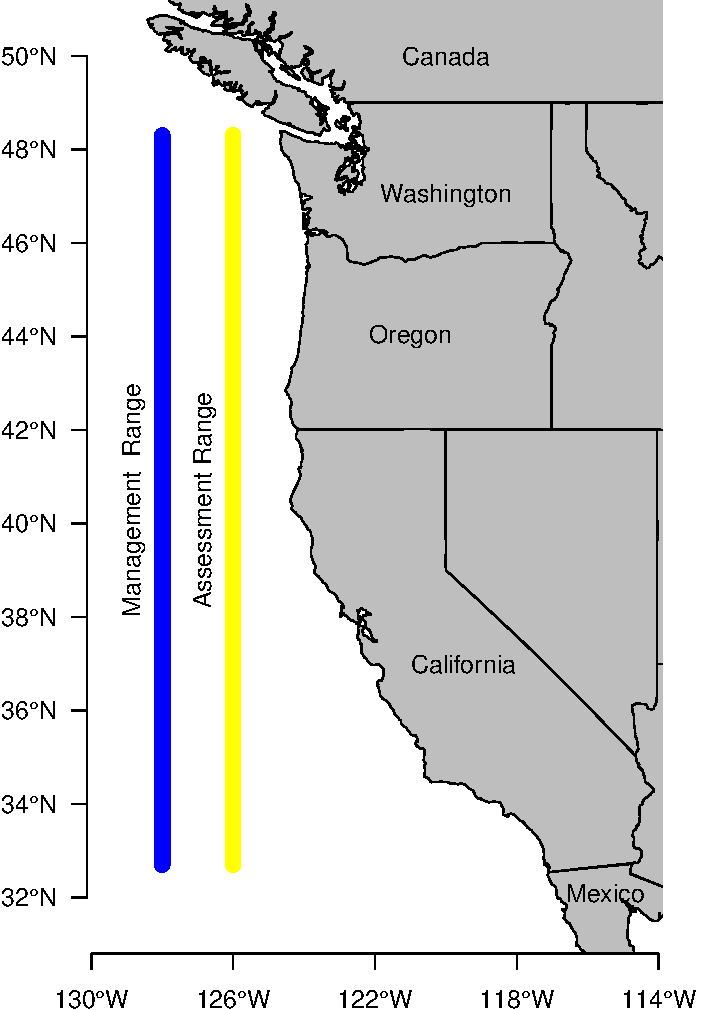
\includegraphics[keepaspectratio]{SAR_USWC_Rougheye_and_Blackspotted_Rockfishes_skeleton_files/figure-pdf/fig-map-1.pdf}}

}

\caption{\label{fig-map}Map of the assessment area.}

\end{figure}%

\begin{figure}[H]

\centering{

\pandocbounded{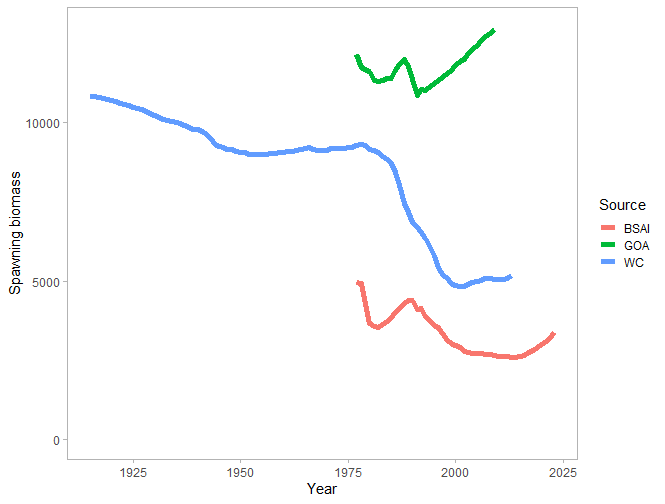
\includegraphics[keepaspectratio]{plots_4_doc/SB_comps.png}}

}

\caption{\label{fig-SO_comp}Estimates of spawning biomass (current
spawning output/unfished spawning output) for the Rougheye/Blackspotted
rockfish complex from the two most recent Alaska (Bering Sea/Aleutian
Islands (BSAI) and Gulf of Alaska (GOA)) and the 2013 U.S. west coast
stock assessment.}

\end{figure}%

\begin{figure}[H]

\centering{

\pandocbounded{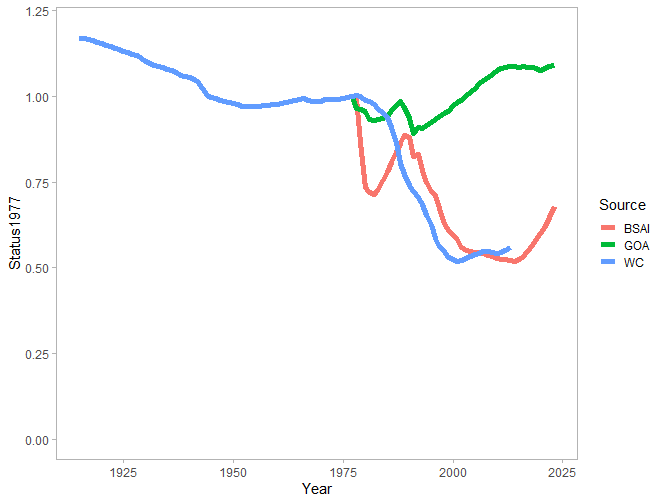
\includegraphics[keepaspectratio]{plots_4_doc/Status_comp.png}}

}

\caption{\label{fig-RSS_comp}Estimates of relative stock size (current
spawning output/unfished spawning output) relative to 1977 (the common
year in all stock assessments compared) for the Rougheye/Blackspotted
rockfish complex from the two most recent Alaska (Bering Sea/Aleutian
Islands (BSAI) and Gulf of Alaska (GOA)) and the 2013 U.S. west coast
stock assessment.}

\end{figure}%

\newpage

\begin{figure}[H]

\centering{

\pandocbounded{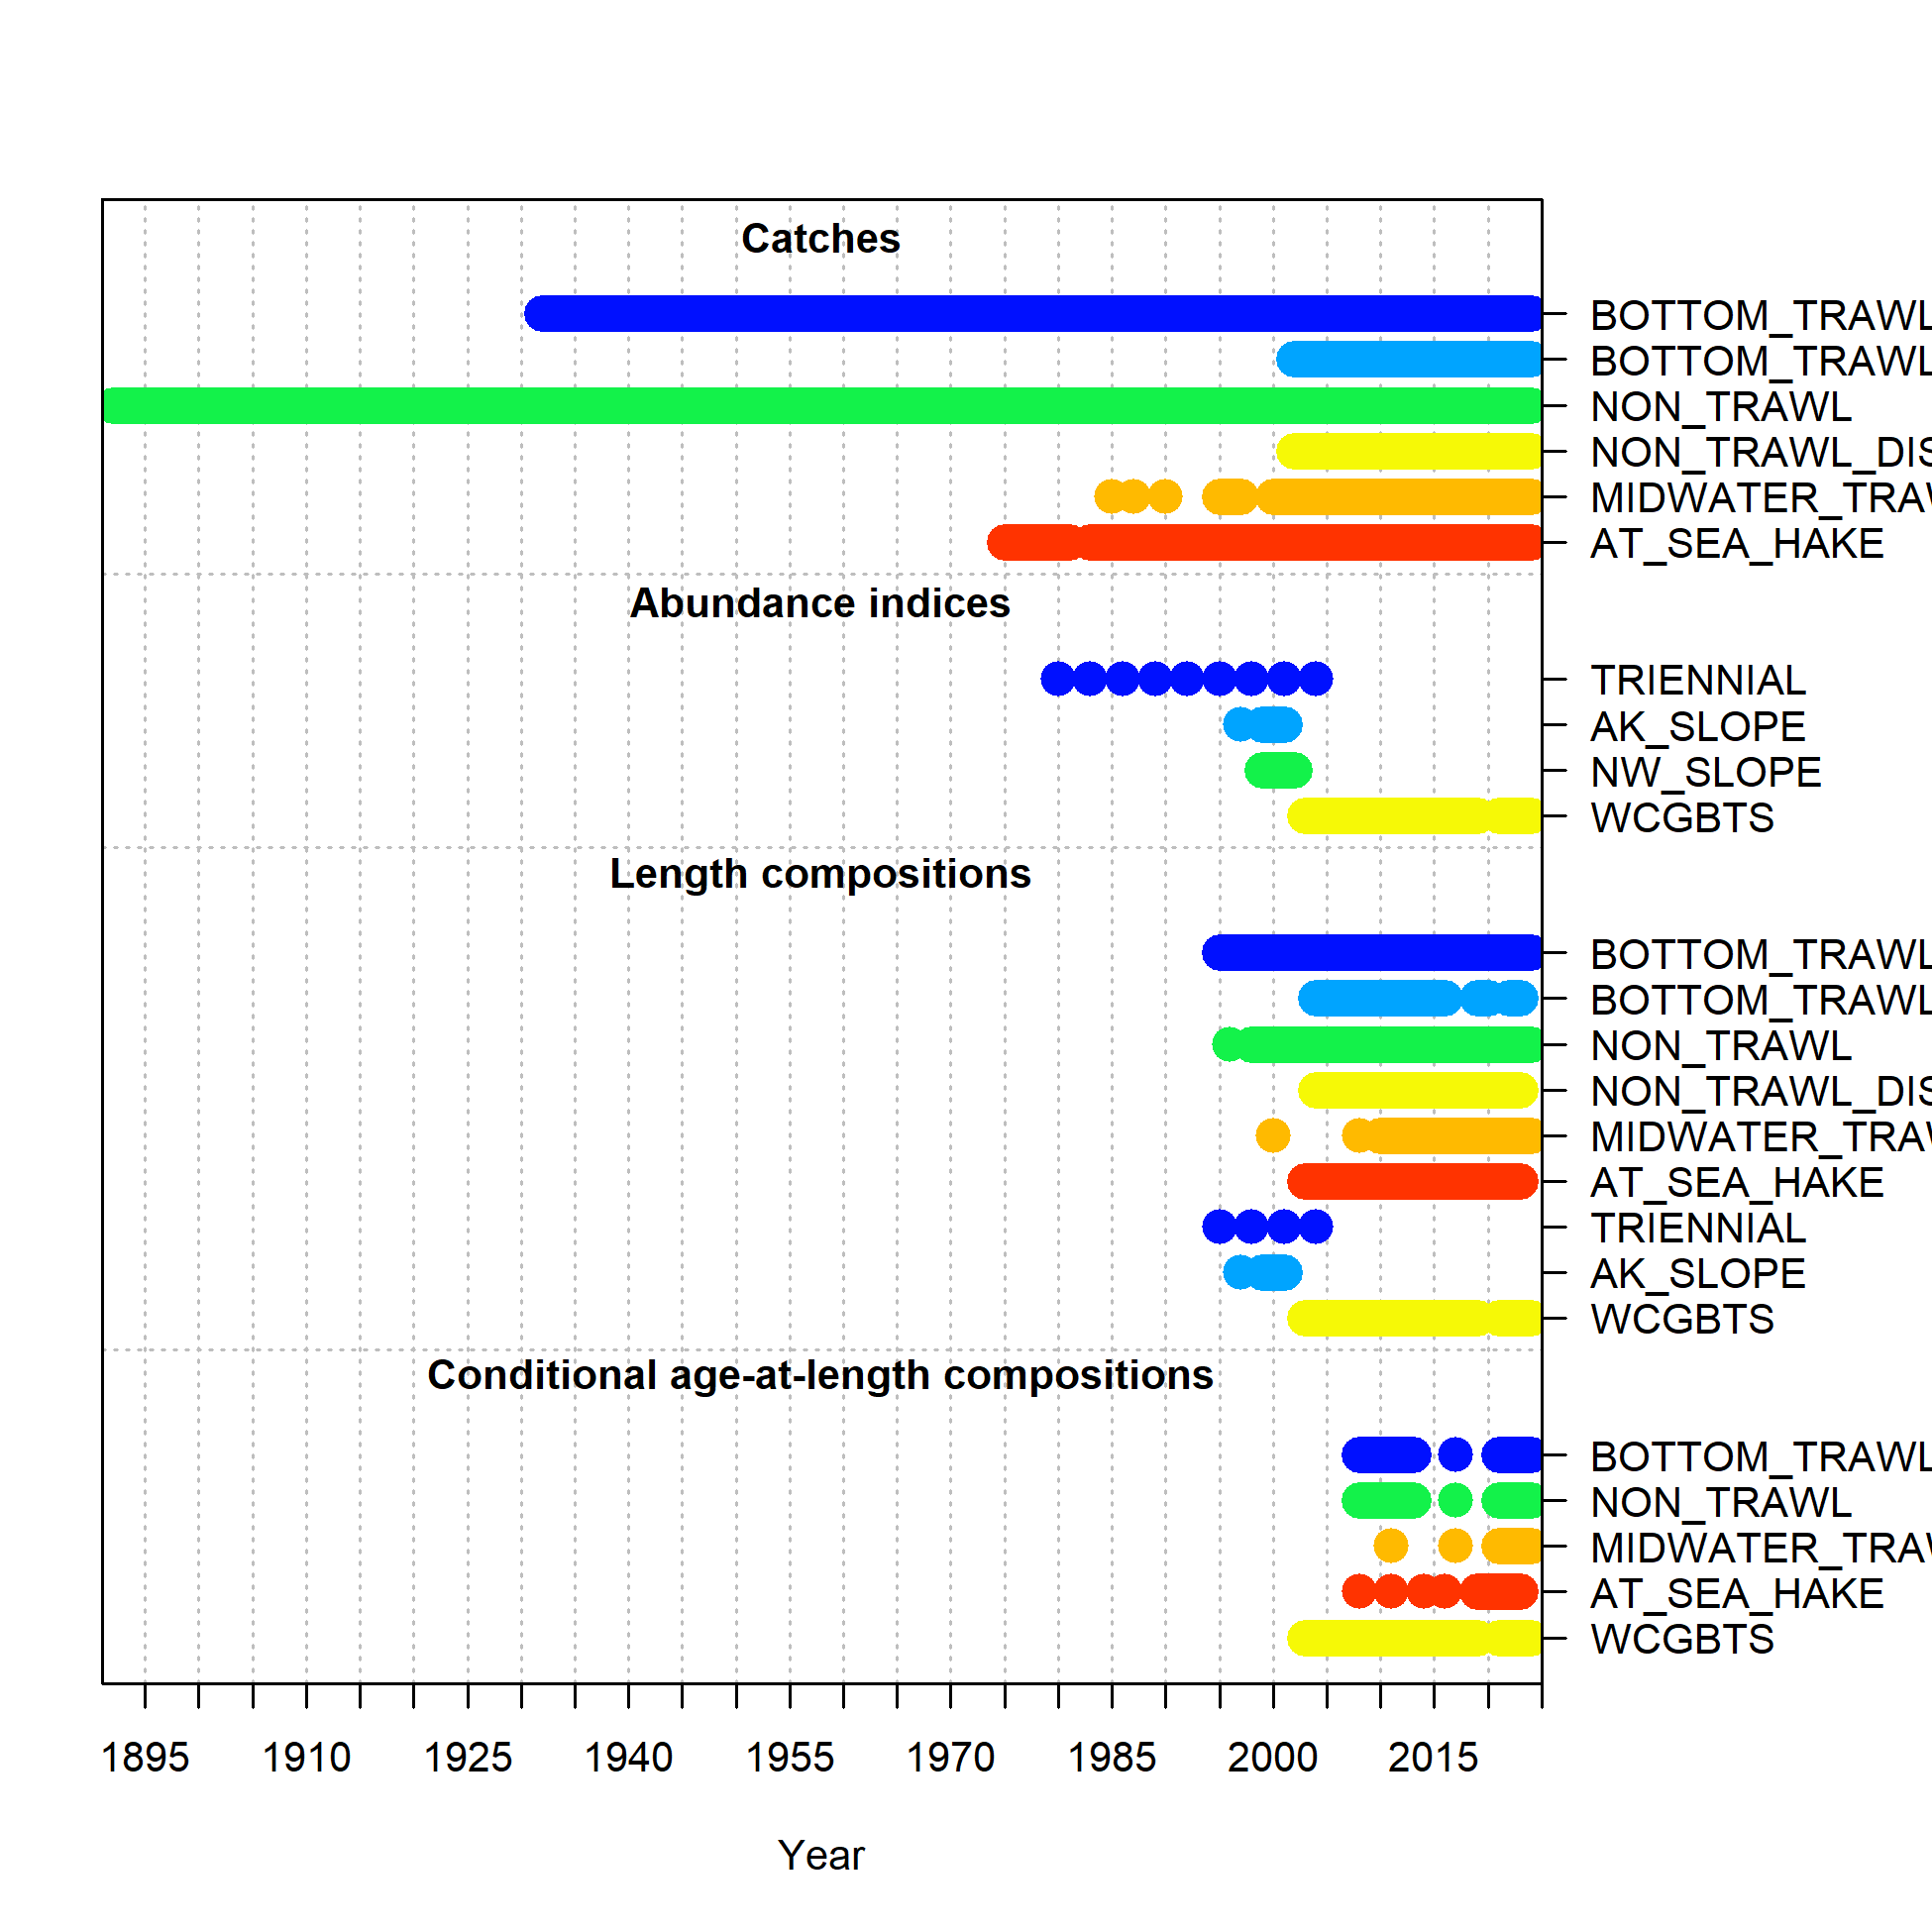
\includegraphics[keepaspectratio]{ref_model/plots/data_plot.png}}

}

\caption{\label{fig-data}Data used in the base model.}

\end{figure}%

\begin{figure}[H]

\centering{

\pandocbounded{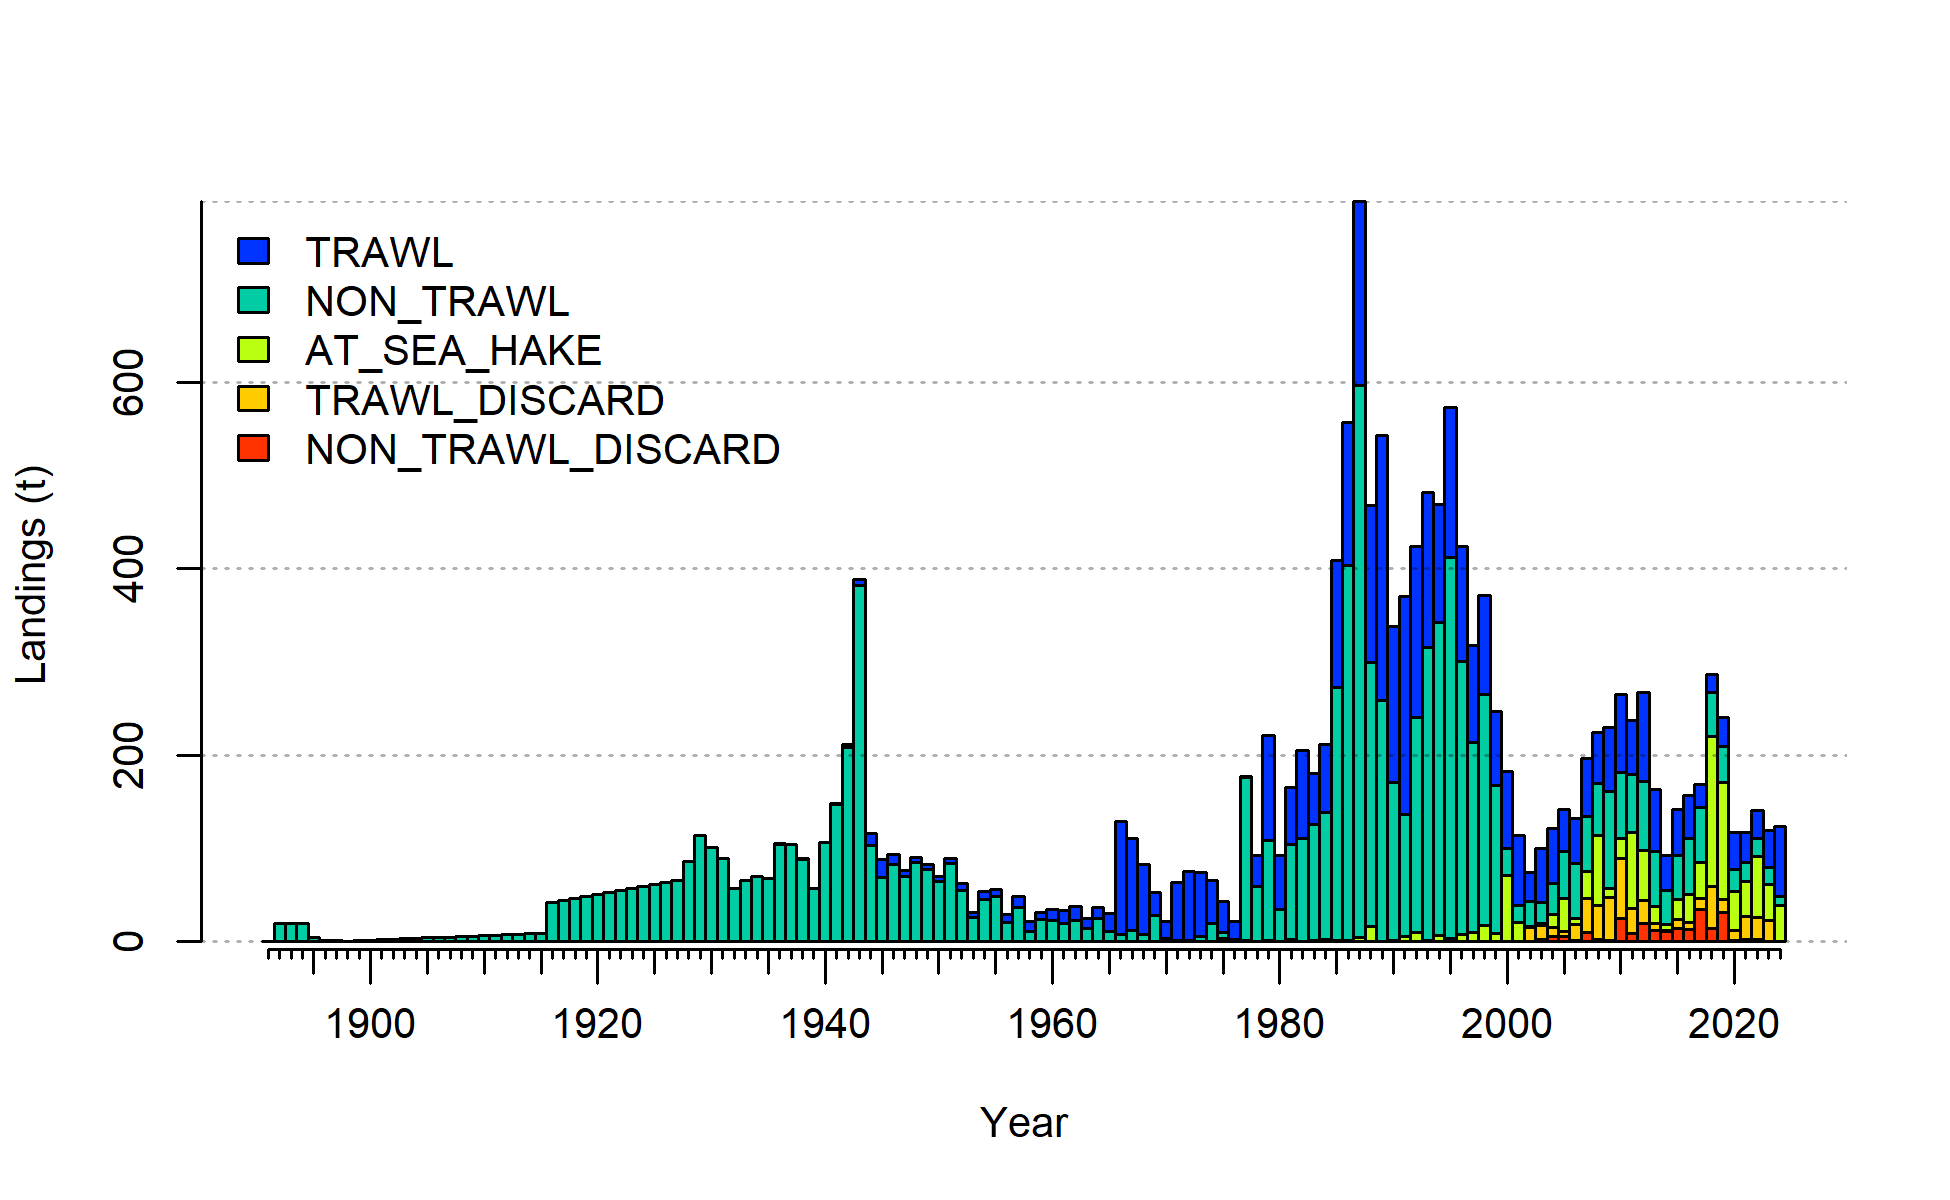
\includegraphics[keepaspectratio]{ref_model/plots/catch2_landings_stacked.png}}

}

\caption{\label{fig-landings}Landings by fleet.}

\end{figure}%

\begin{figure}[H]

\centering{

\pandocbounded{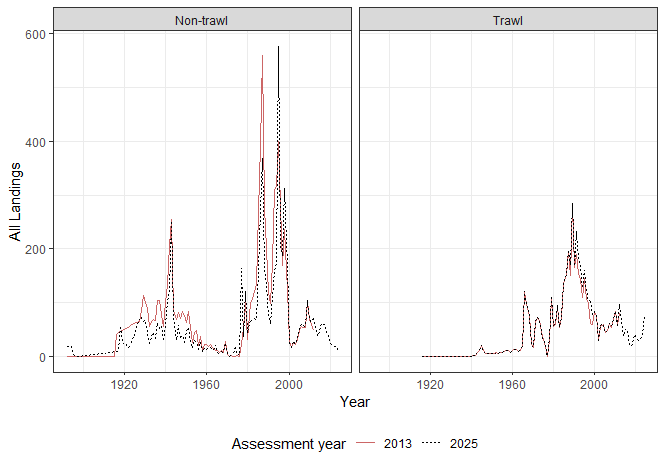
\includegraphics[keepaspectratio]{plots_4_doc/Catch_comp_all.png}}

}

\caption{\label{fig-Ct_All}Landings across all states for non-trawl and
trawl fisheries compared between the 2013 assessment and updated
landings for the 2025 stock assessment model.}

\end{figure}%

\begin{figure}[H]

\centering{

\pandocbounded{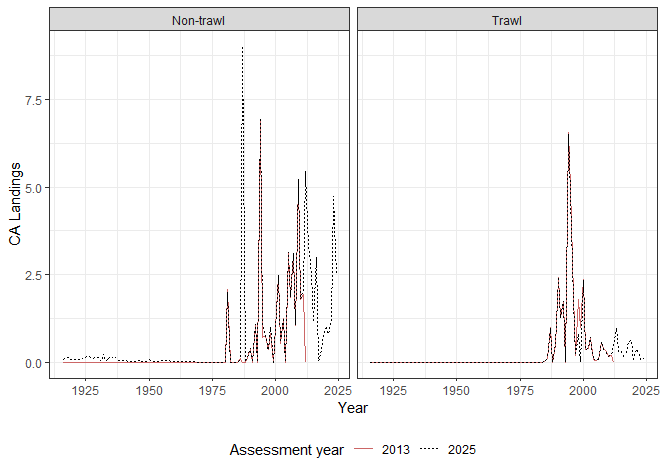
\includegraphics[keepaspectratio]{plots_4_doc/Catch_comp_CA.png}}

}

\caption{\label{fig-Ct_CA}California state landings for non-trawl and
trawl fisheries compared between the 2013 assessment and updated
landings for the 2025 stock assessment model.}

\end{figure}%

\begin{figure}[H]

\centering{

\pandocbounded{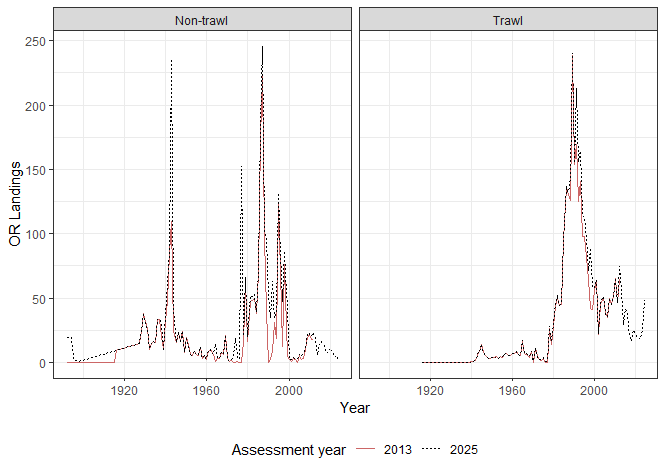
\includegraphics[keepaspectratio]{plots_4_doc/Catch_comp_OR.png}}

}

\caption{\label{fig-Ct_OR}Oregon state landings for non-trawl and trawl
fisheries compared between the 2013 assessment and updated landings for
the 2025 stock assessment model.}

\end{figure}%

\begin{figure}[H]

\centering{

\pandocbounded{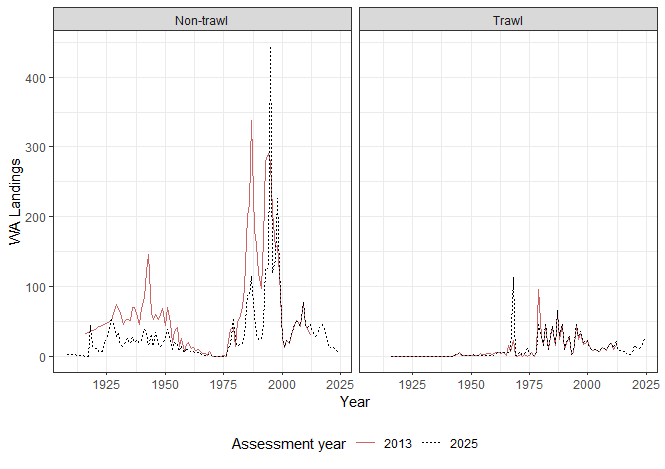
\includegraphics[keepaspectratio]{plots_4_doc/Catch_comp_WA.png}}

}

\caption{\label{fig-Ct_WA}WA. Washington state landings for non-trawl
and trawl fisheries compared between the 2013 assessment and updated
landings for the 2025 stock assessment model.}

\end{figure}%

\begin{figure}[H]

\centering{

\pandocbounded{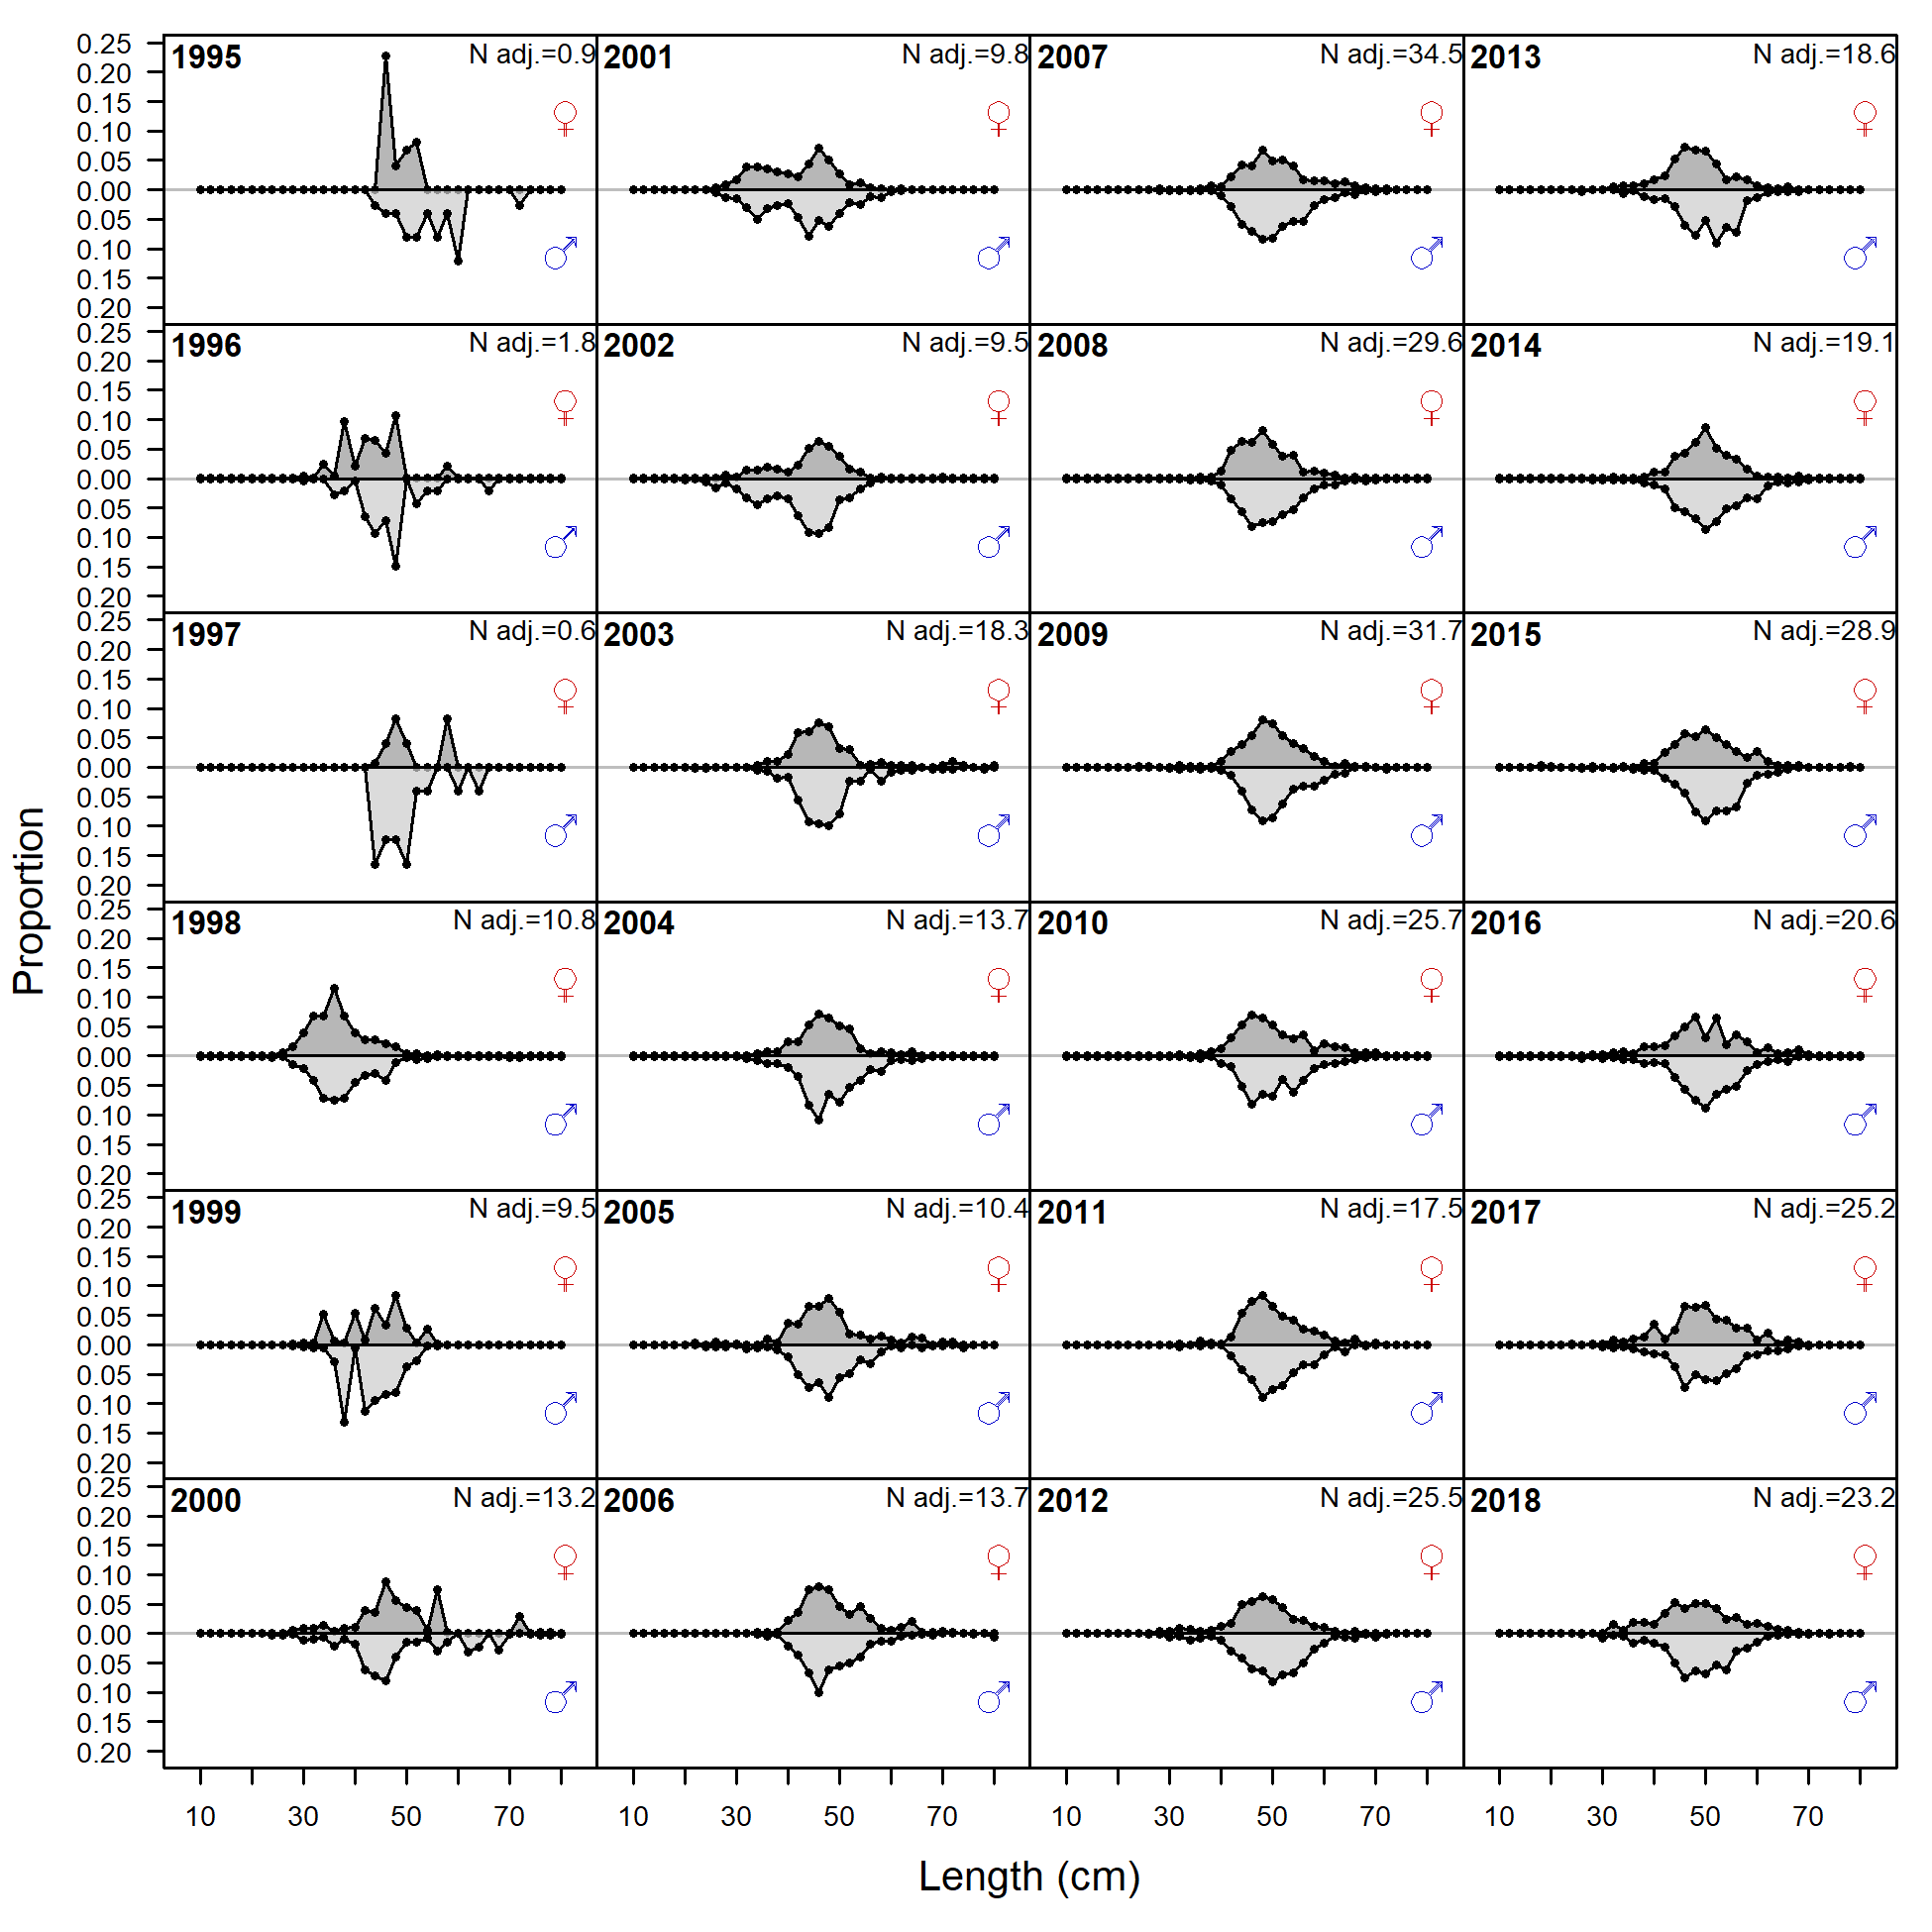
\includegraphics[keepaspectratio]{ref_model/plots/comp_lendat_flt1mkt0_page1.png}}

}

\caption{\label{fig-length_flt1_1}Length composition data for bottom
trawl fleet.}

\end{figure}%

\begin{figure}[H]

\centering{

\pandocbounded{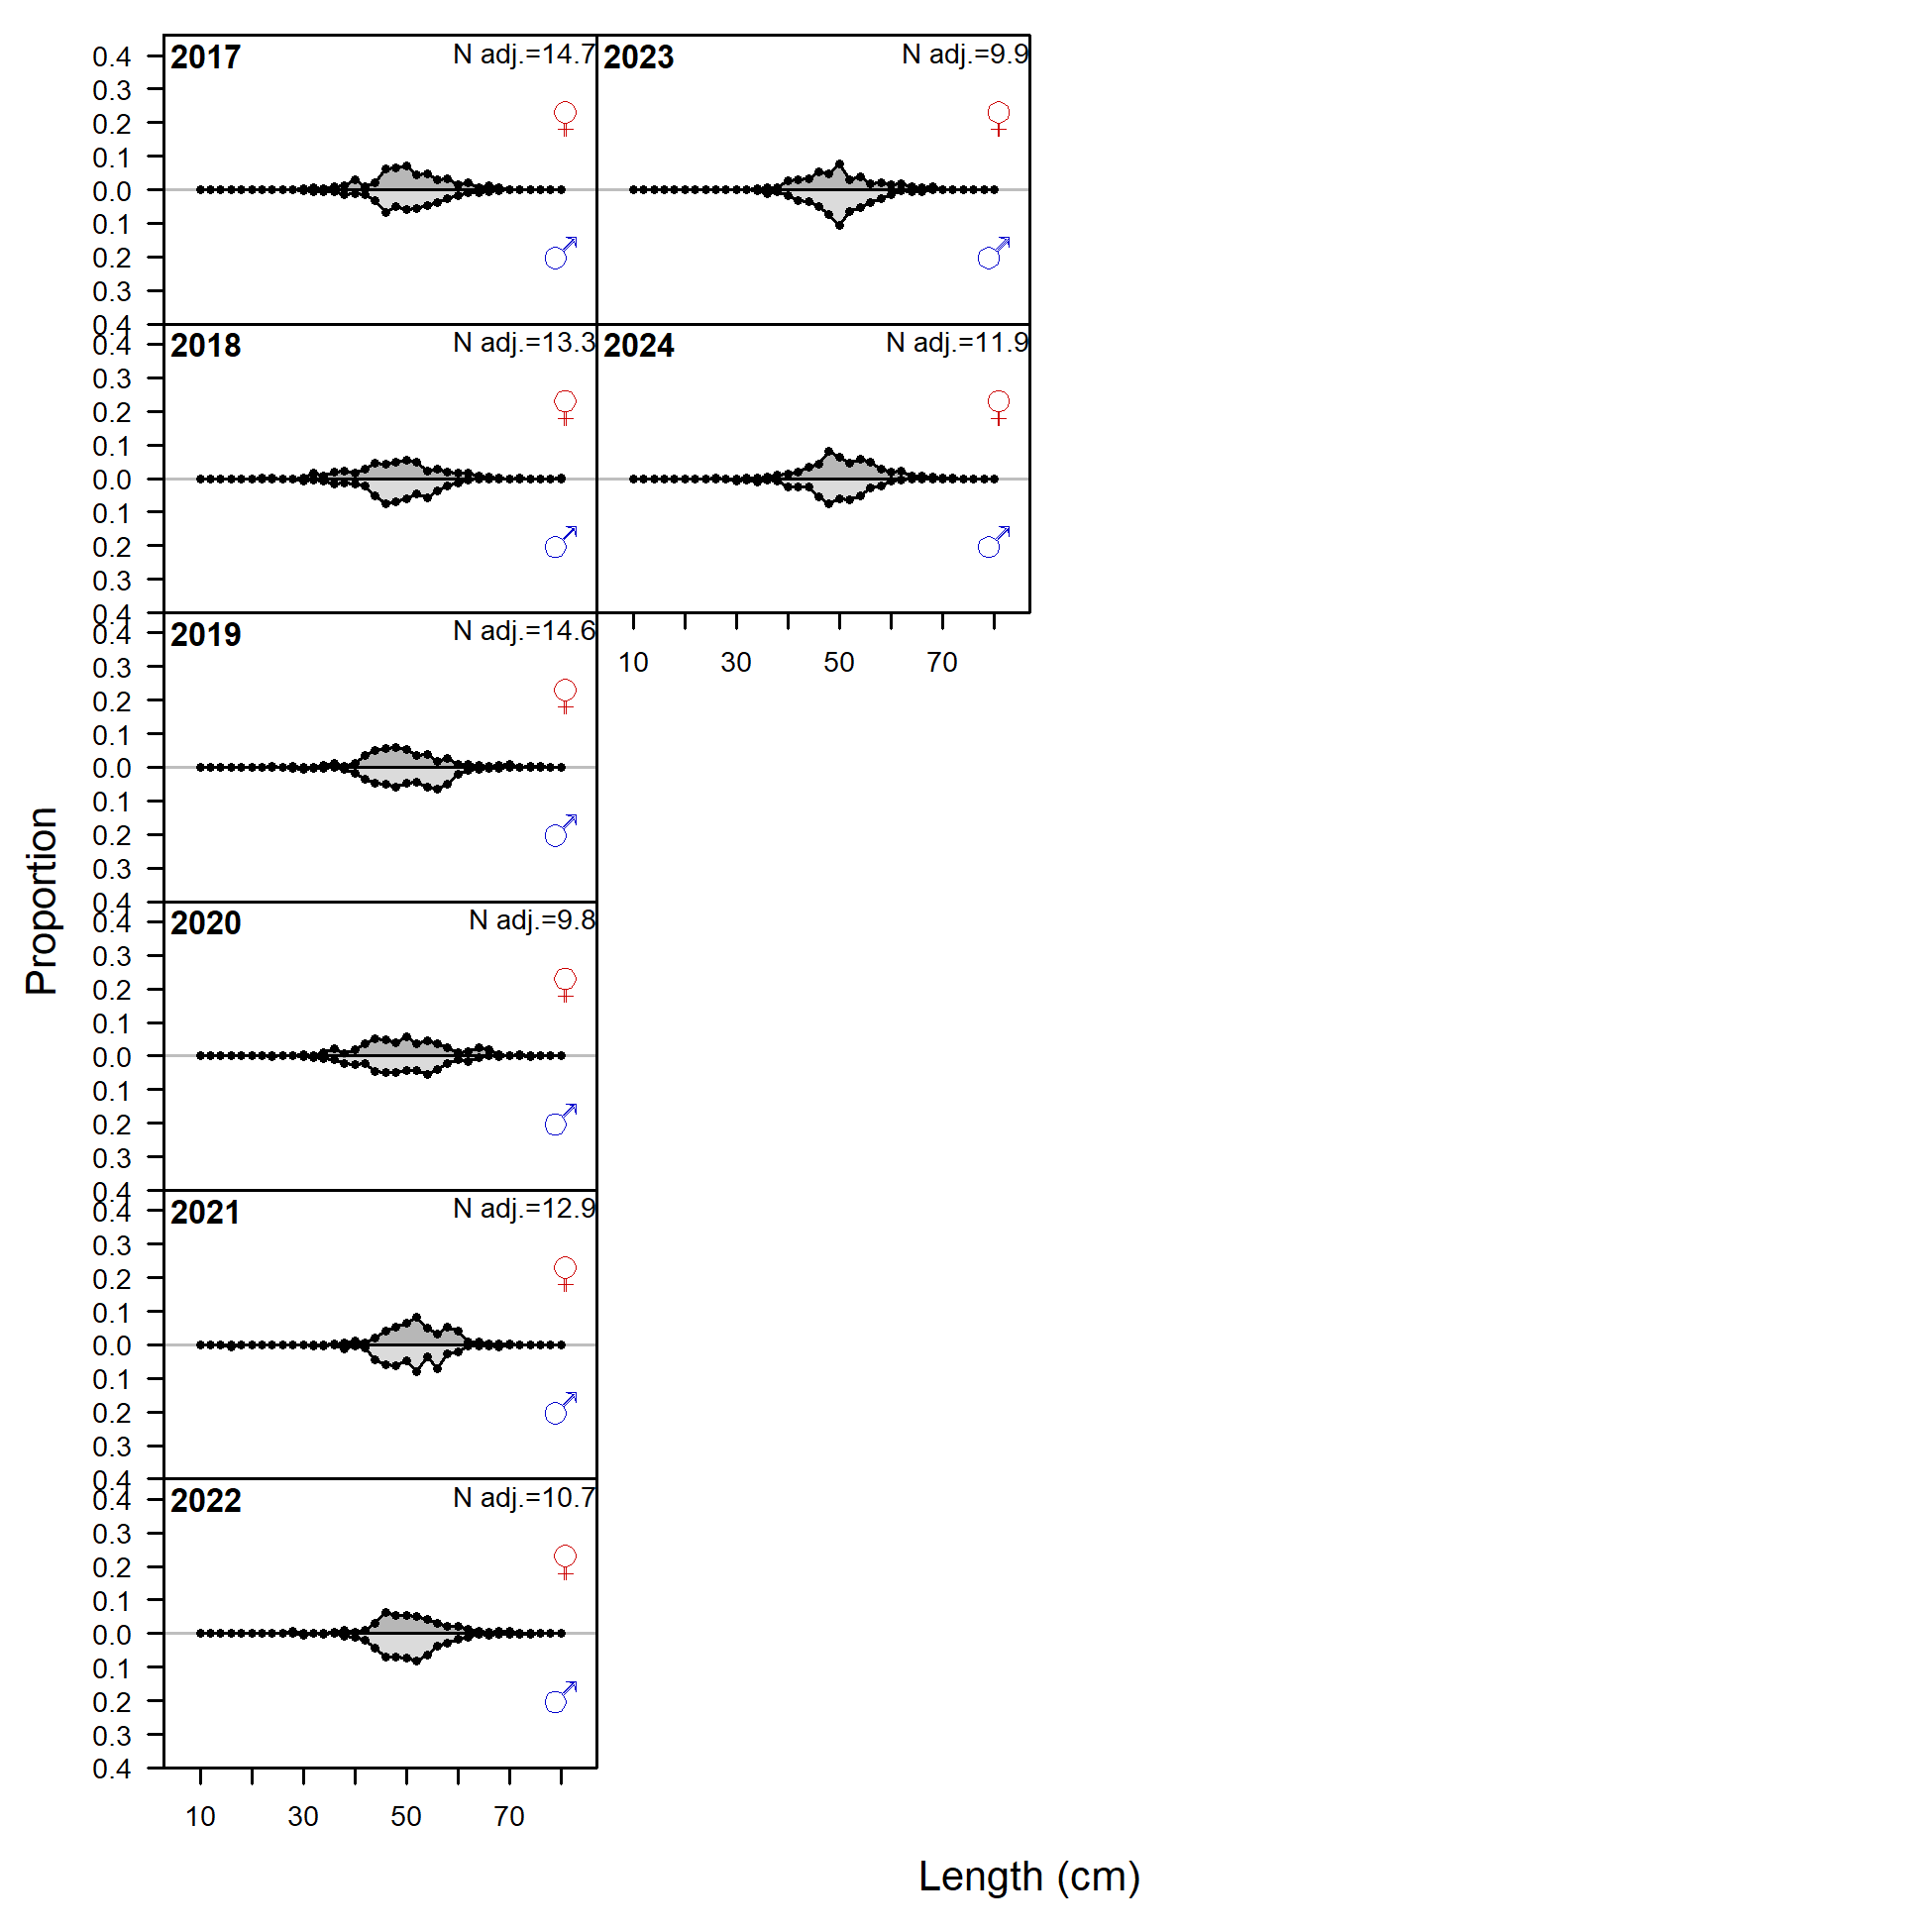
\includegraphics[keepaspectratio]{ref_model/plots/comp_lendat_flt1mkt0_page2.png}}

}

\caption{\label{fig-length_flt1_2}Length composition data for bottom
trawl fleet, continued.}

\end{figure}%

\begin{figure}[H]

\centering{

\pandocbounded{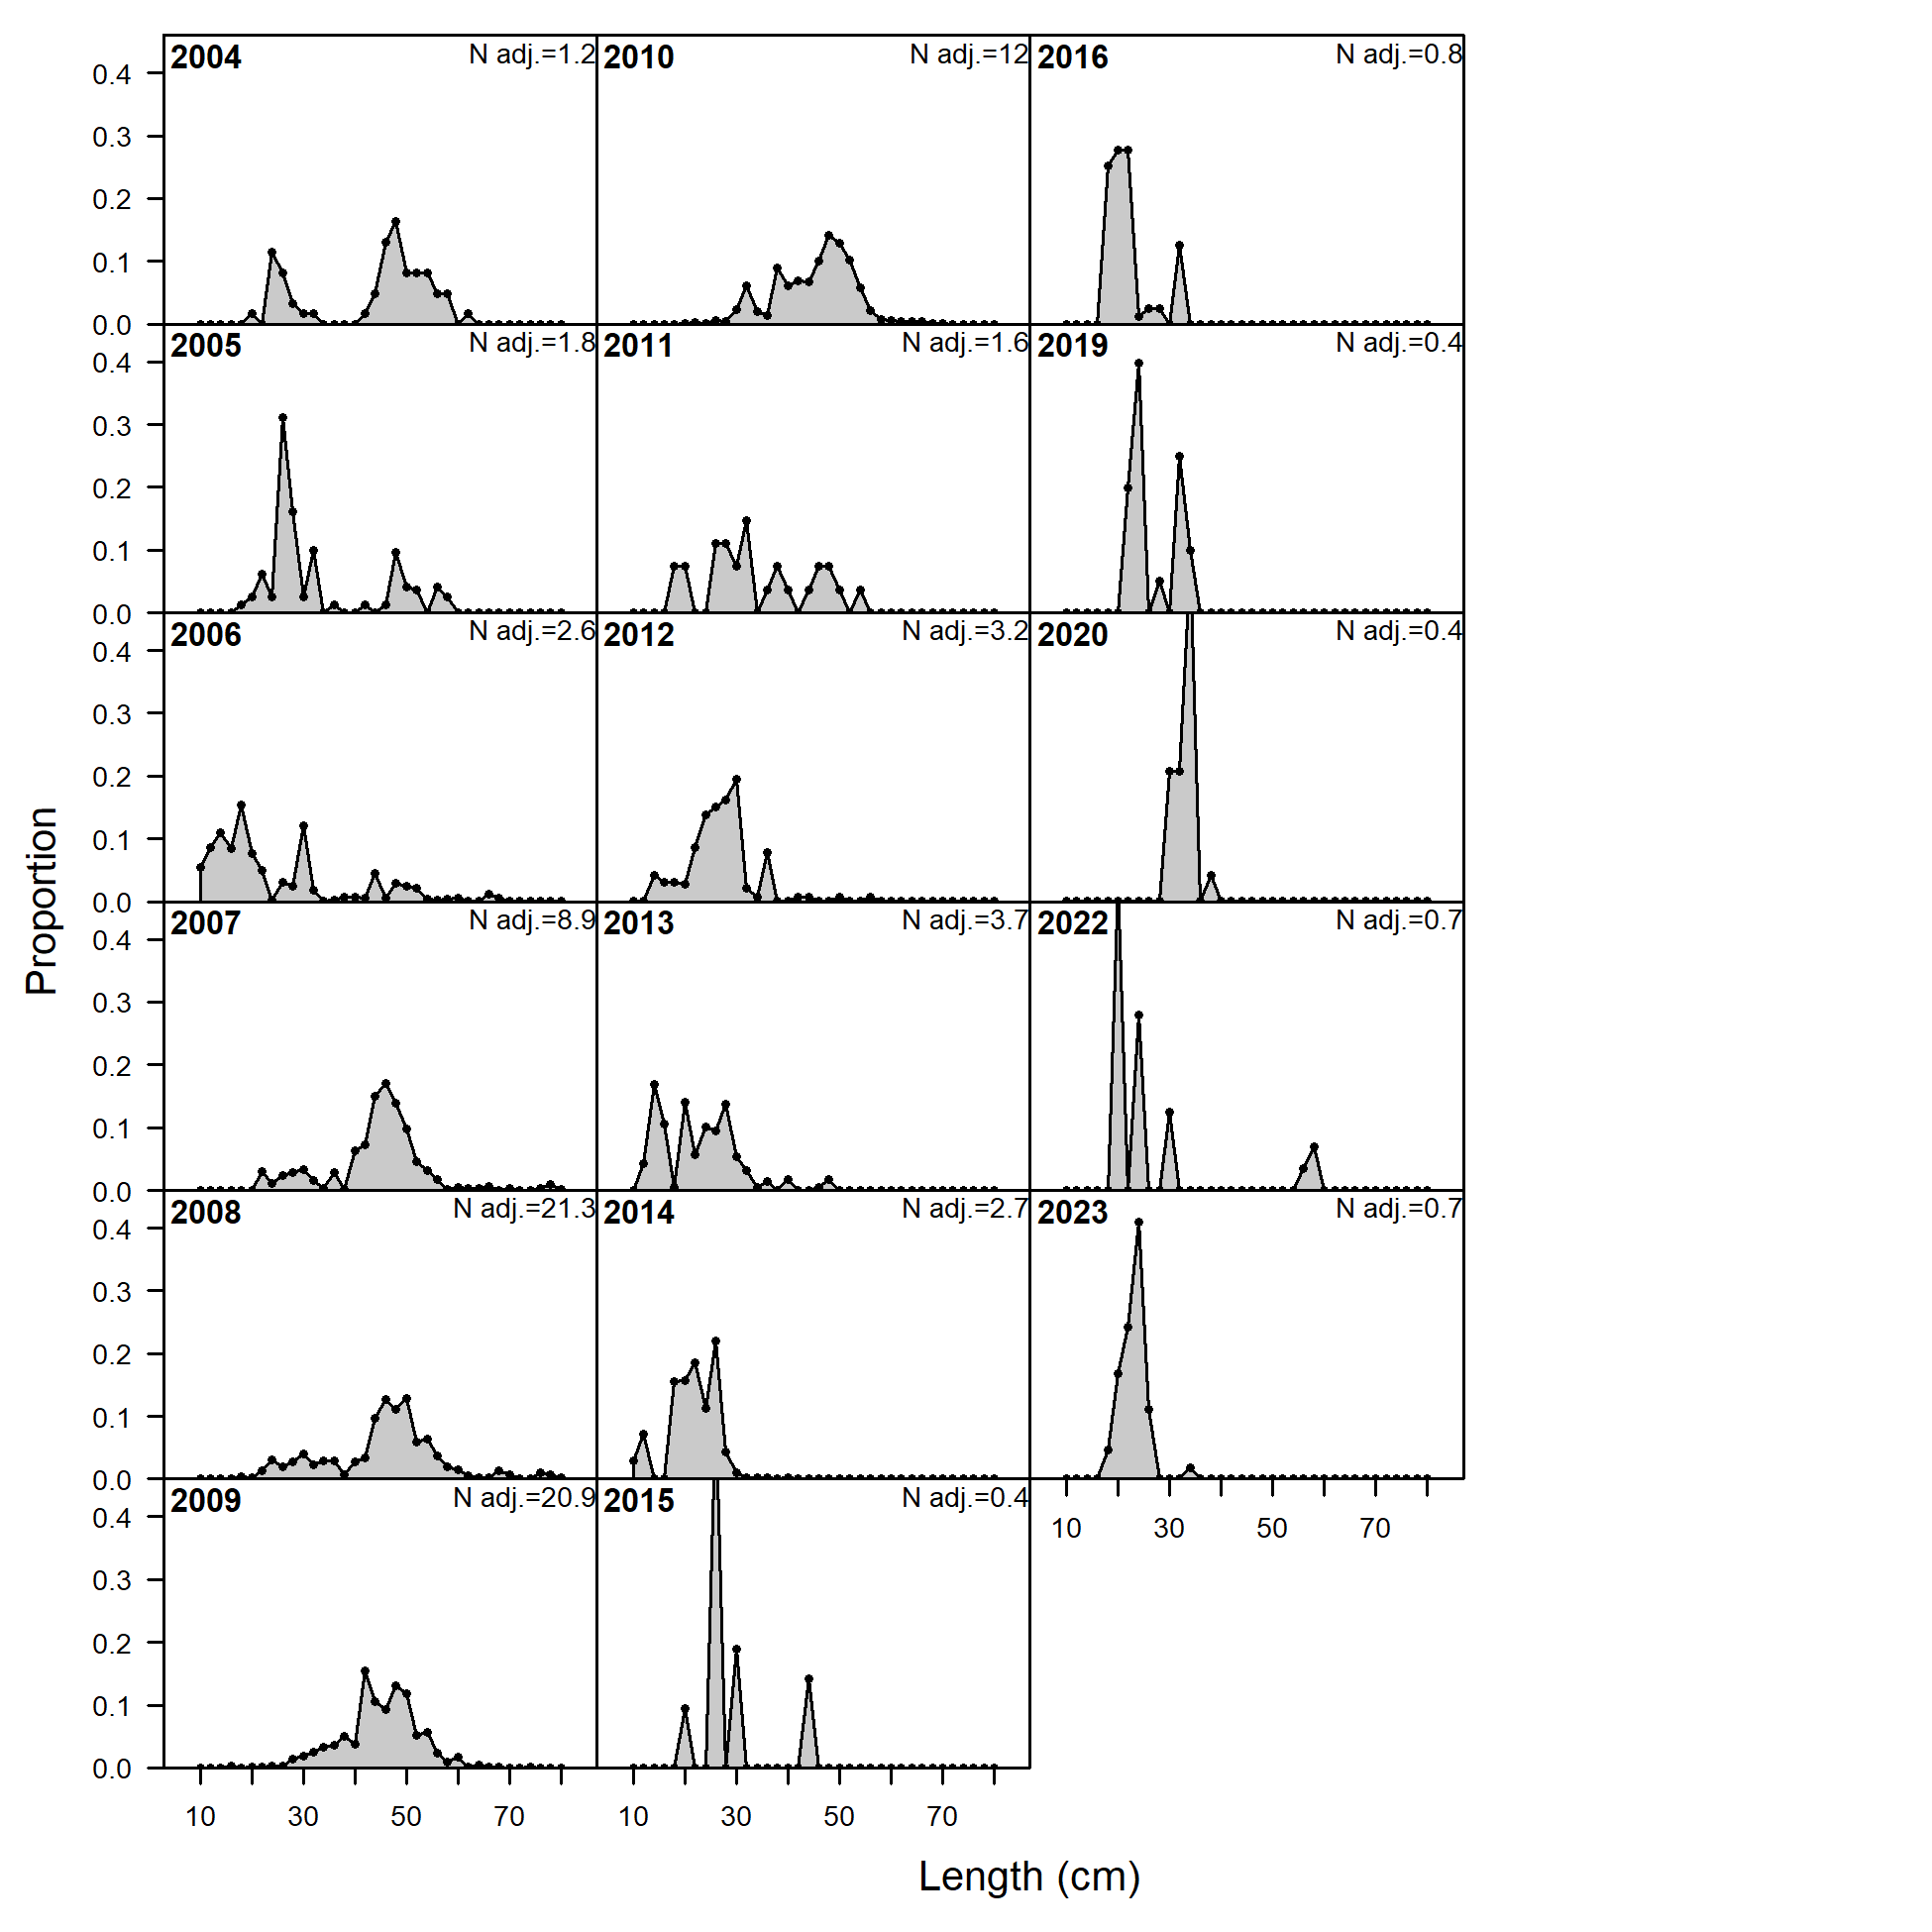
\includegraphics[keepaspectratio]{ref_model/plots/comp_lendat_flt2mkt0.png}}

}

\caption{\label{fig-length_flt2}Length composition data for bottom trawl
discard fleet.}

\end{figure}%

\begin{figure}[H]

\centering{

\pandocbounded{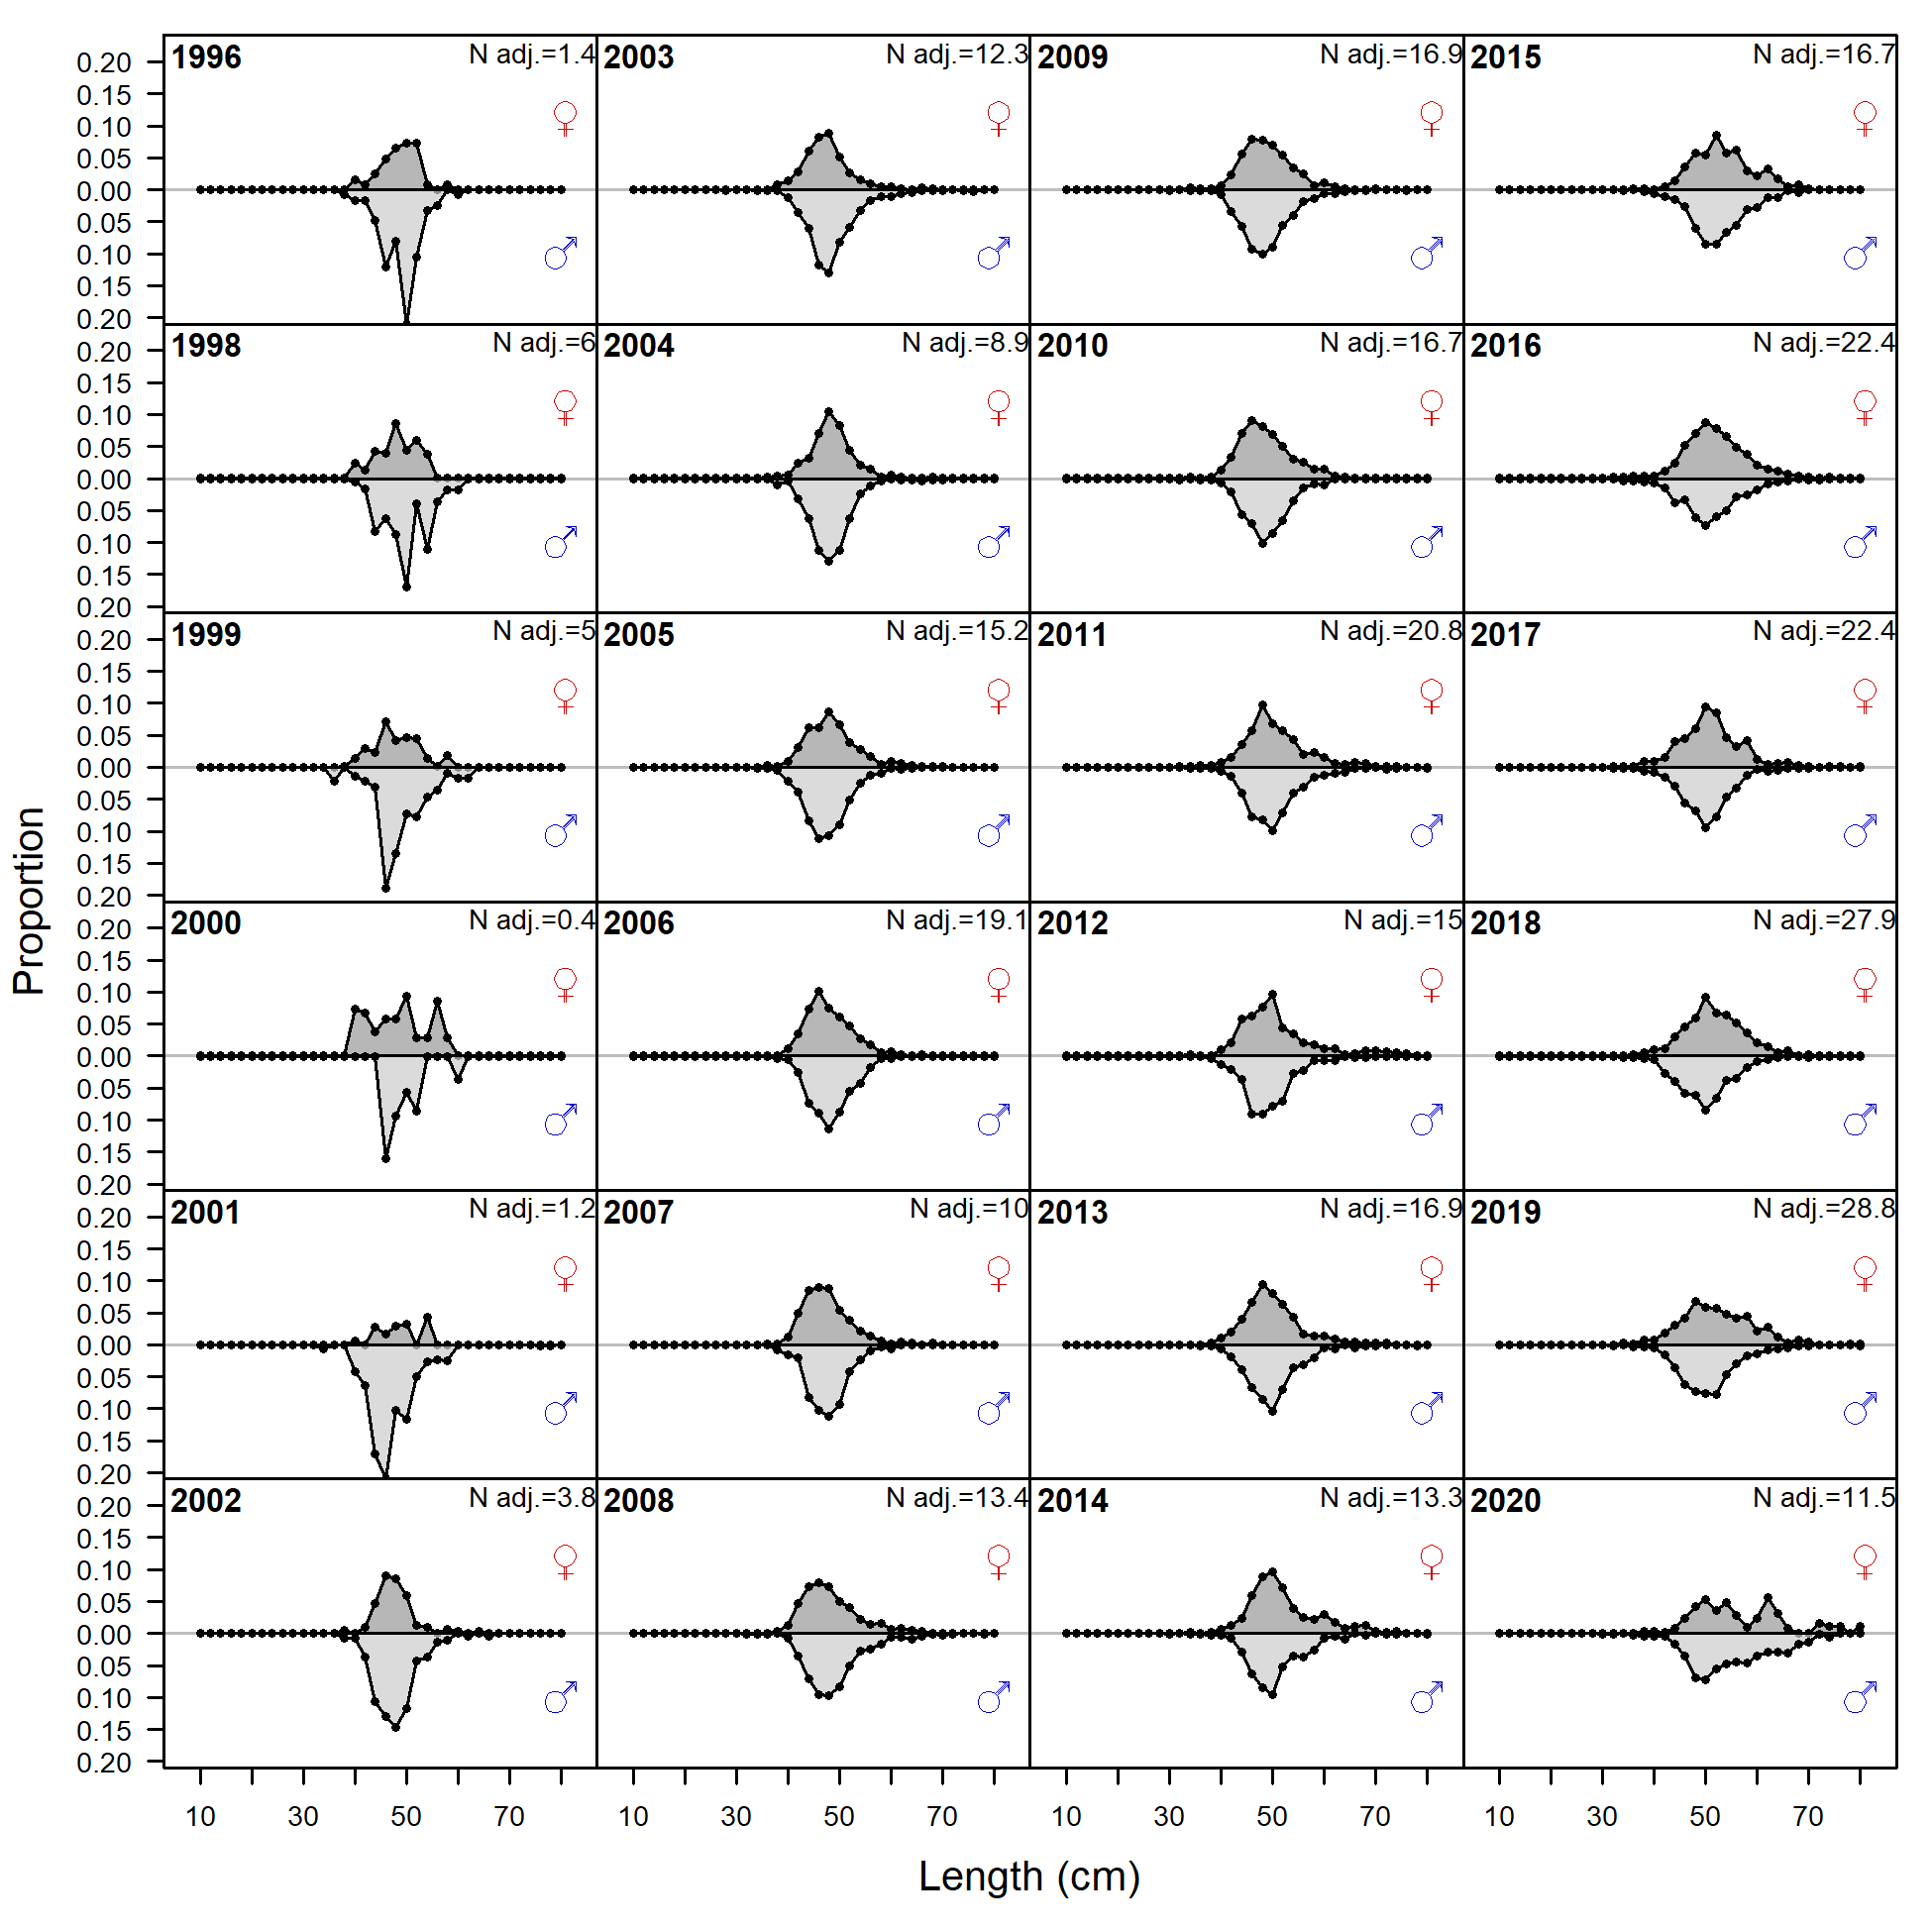
\includegraphics[keepaspectratio]{ref_model/plots/comp_lendat_flt3mkt0_page1.png}}

}

\caption{\label{fig-length_flt3_1}Length composition data for non-trawl
fleet.}

\end{figure}%

\begin{figure}[H]

\centering{

\pandocbounded{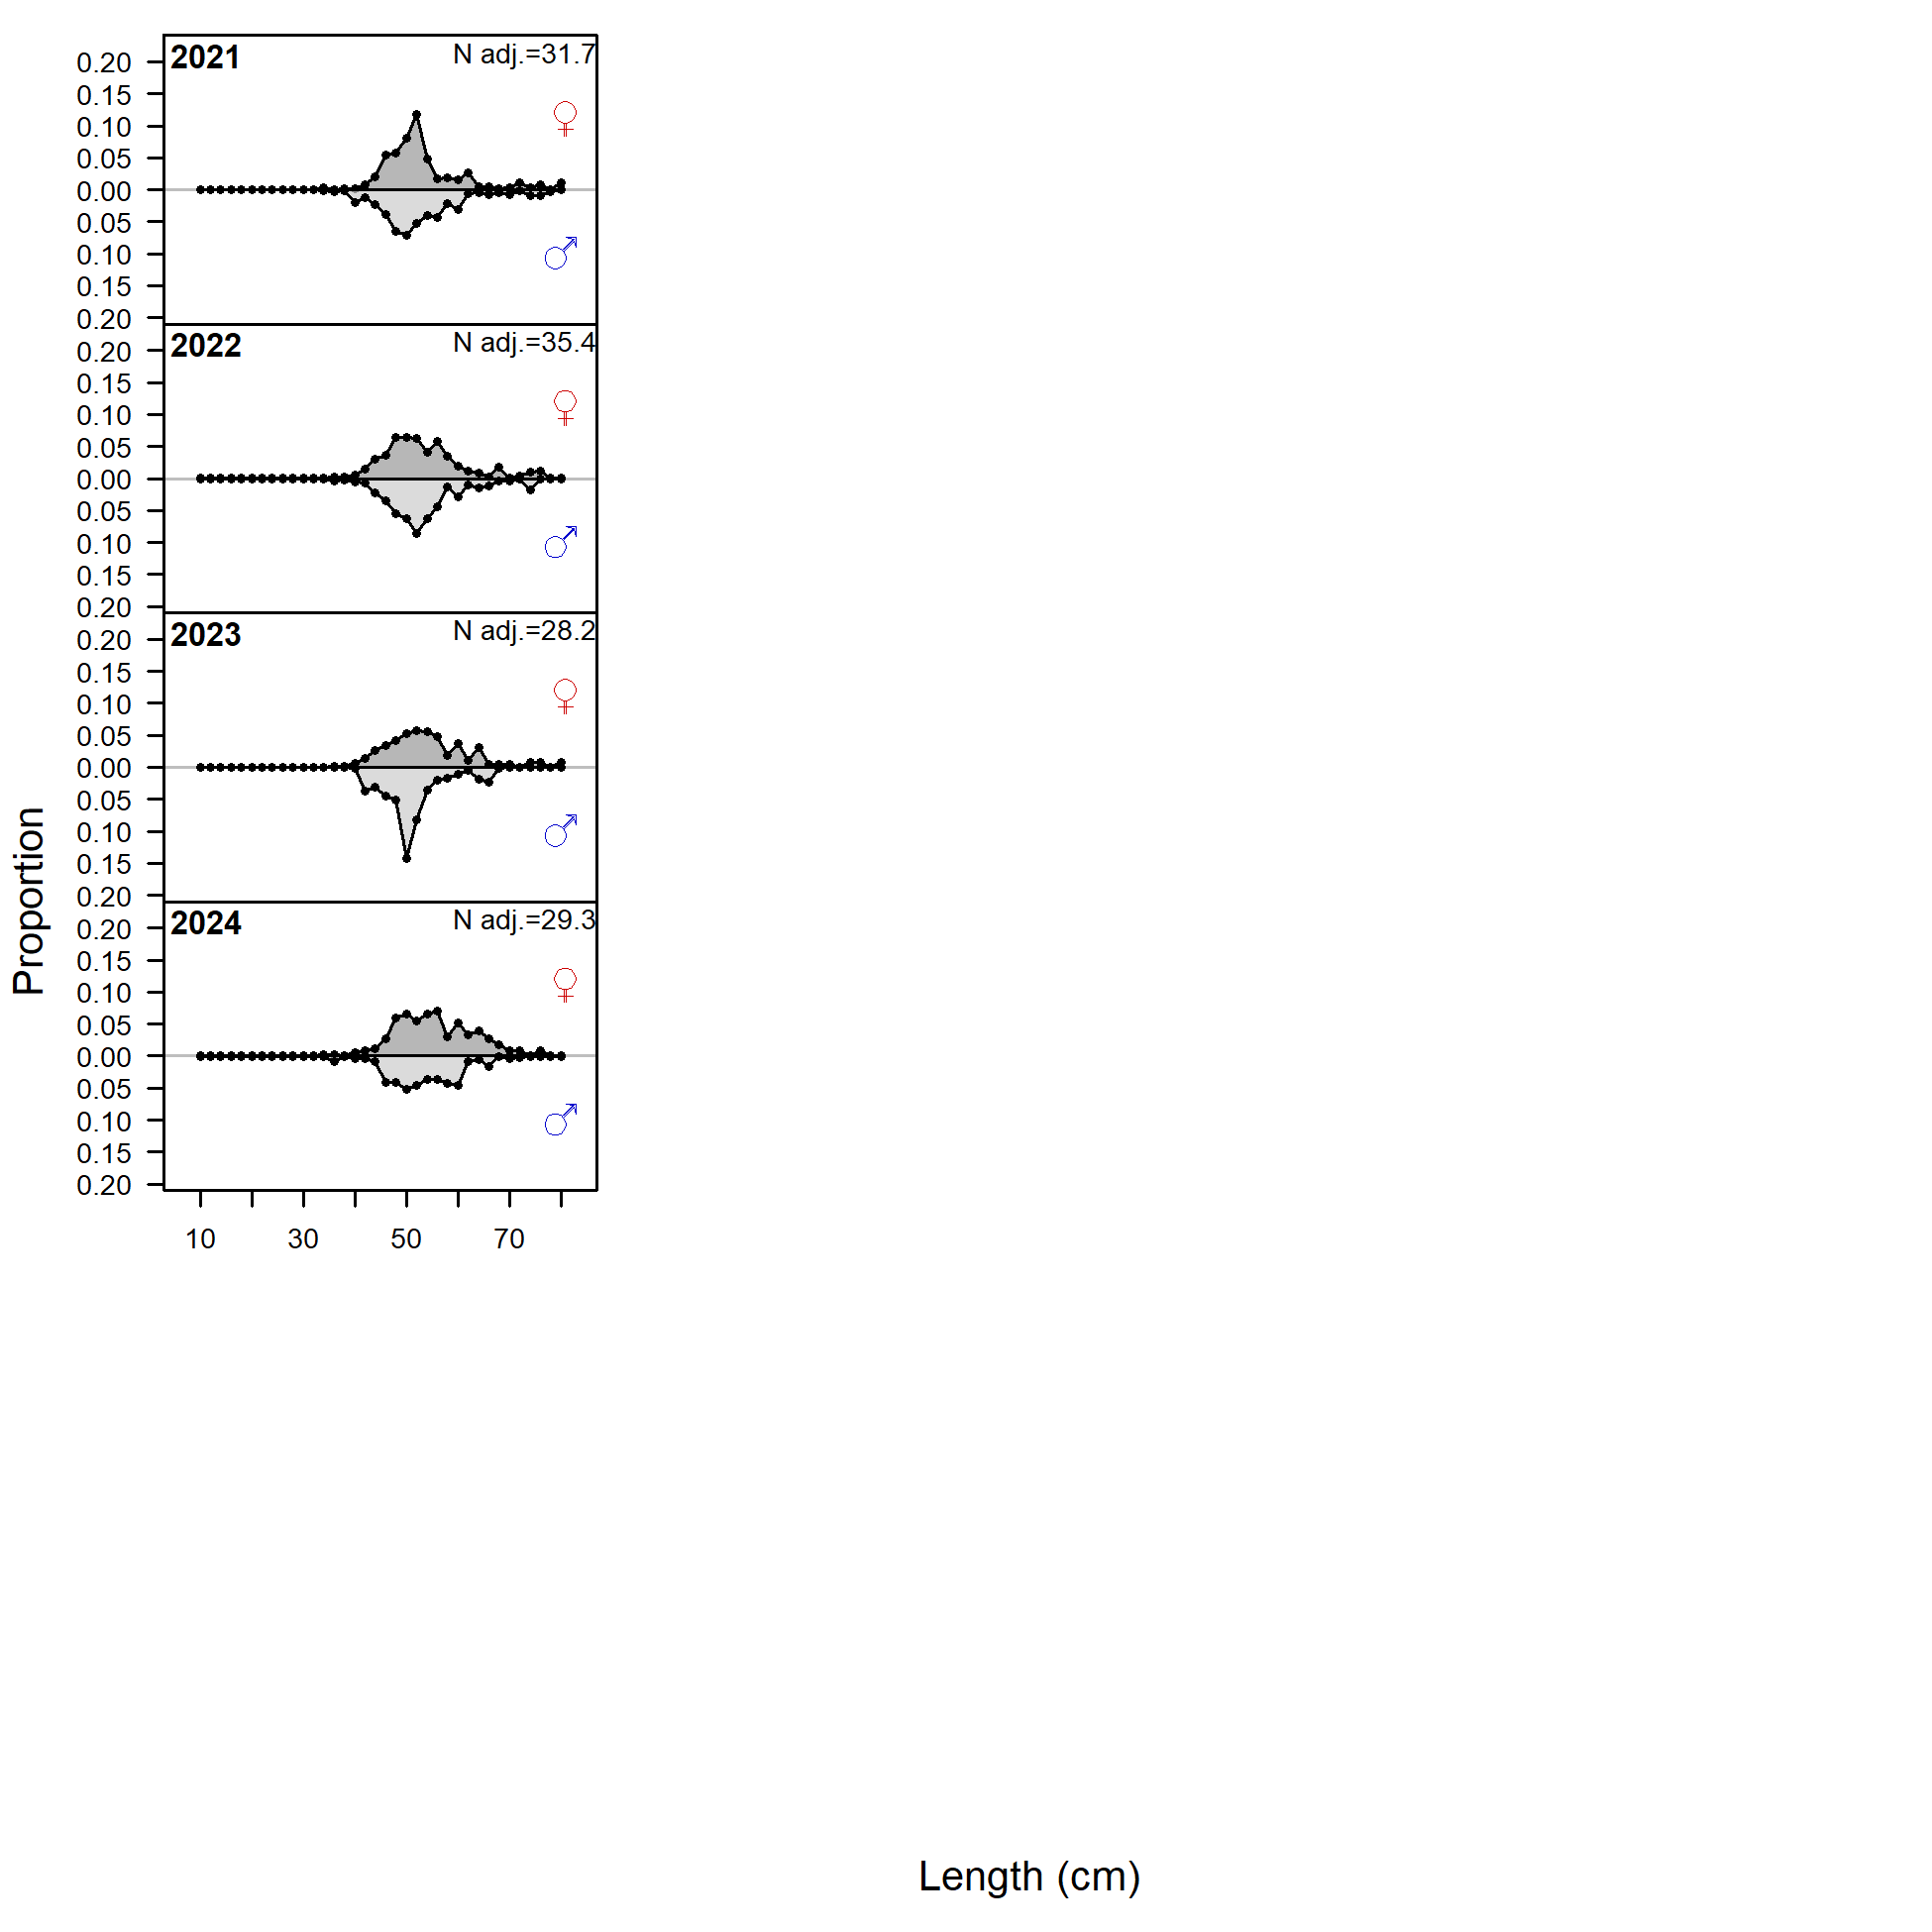
\includegraphics[keepaspectratio]{ref_model/plots/comp_lendat_flt3mkt0_page2.png}}

}

\caption{\label{fig-length_flt3_2}Length composition data for non-trawl
fleet, continued.}

\end{figure}%

\begin{figure}[H]

\centering{

\pandocbounded{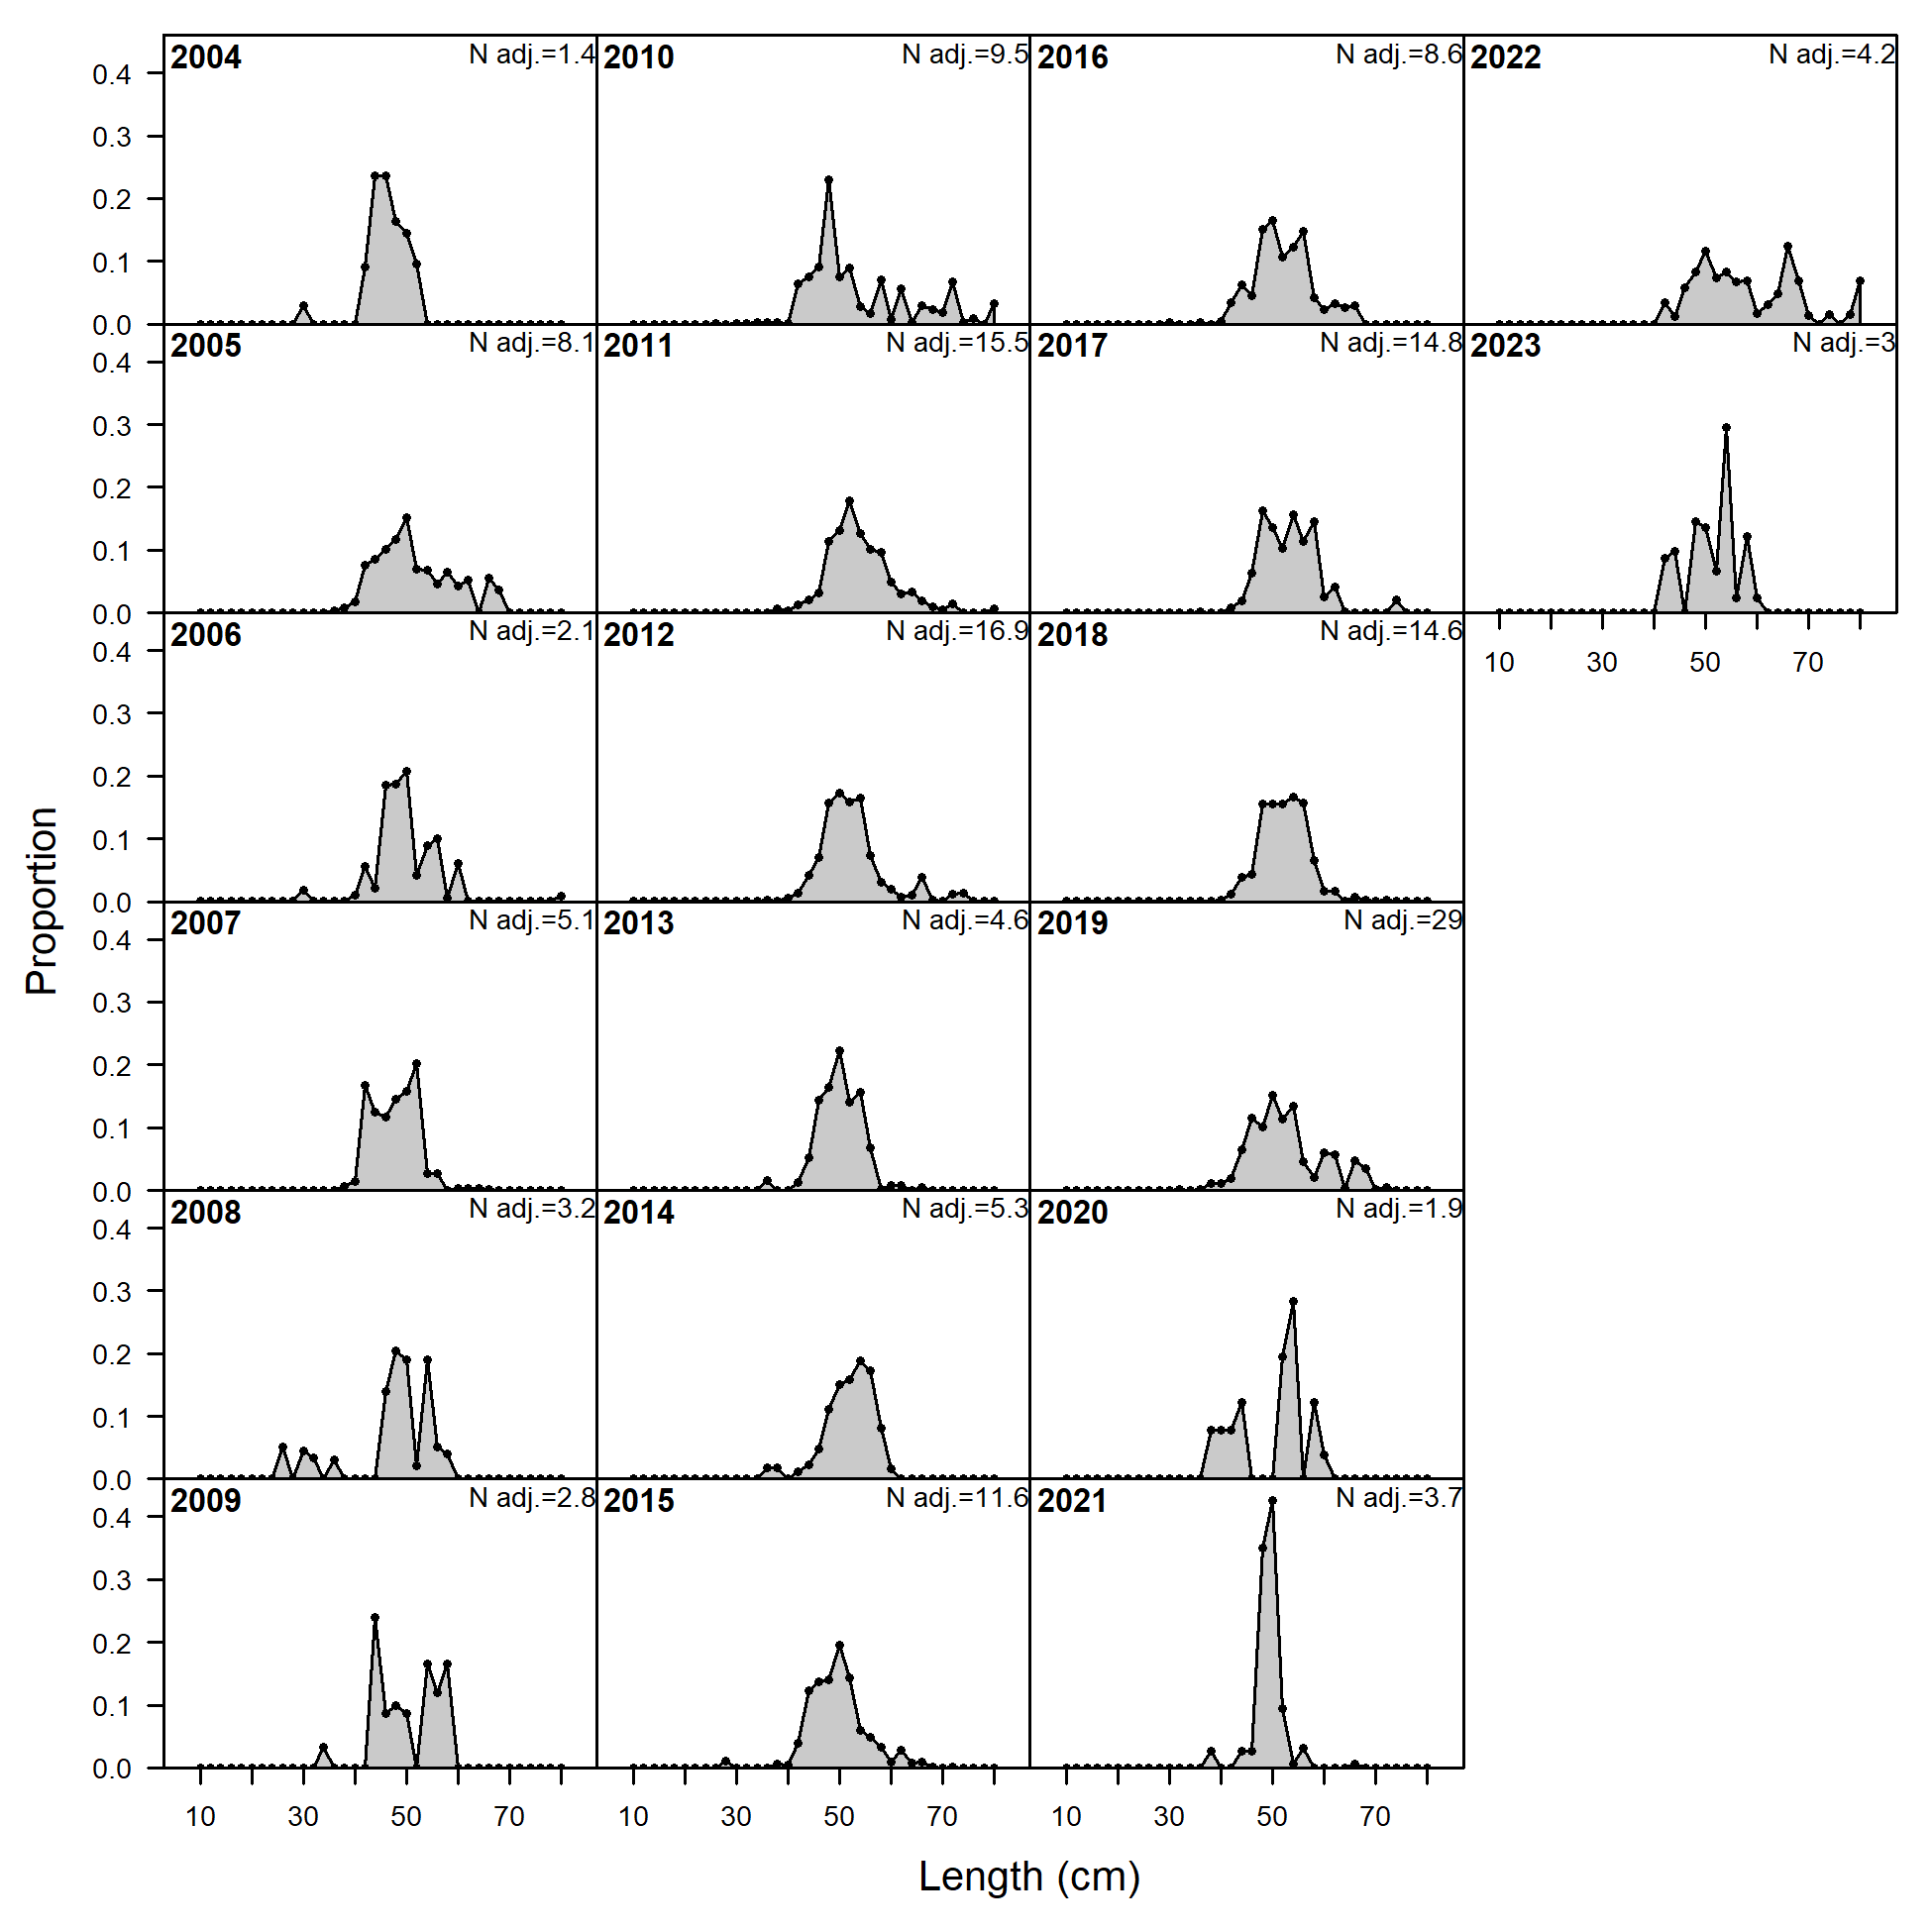
\includegraphics[keepaspectratio]{ref_model/plots/comp_lendat_flt4mkt0.png}}

}

\caption{\label{fig-length_flt4}Length composition data for non-trawl
discard fleet.}

\end{figure}%

\begin{figure}[H]

\centering{

\pandocbounded{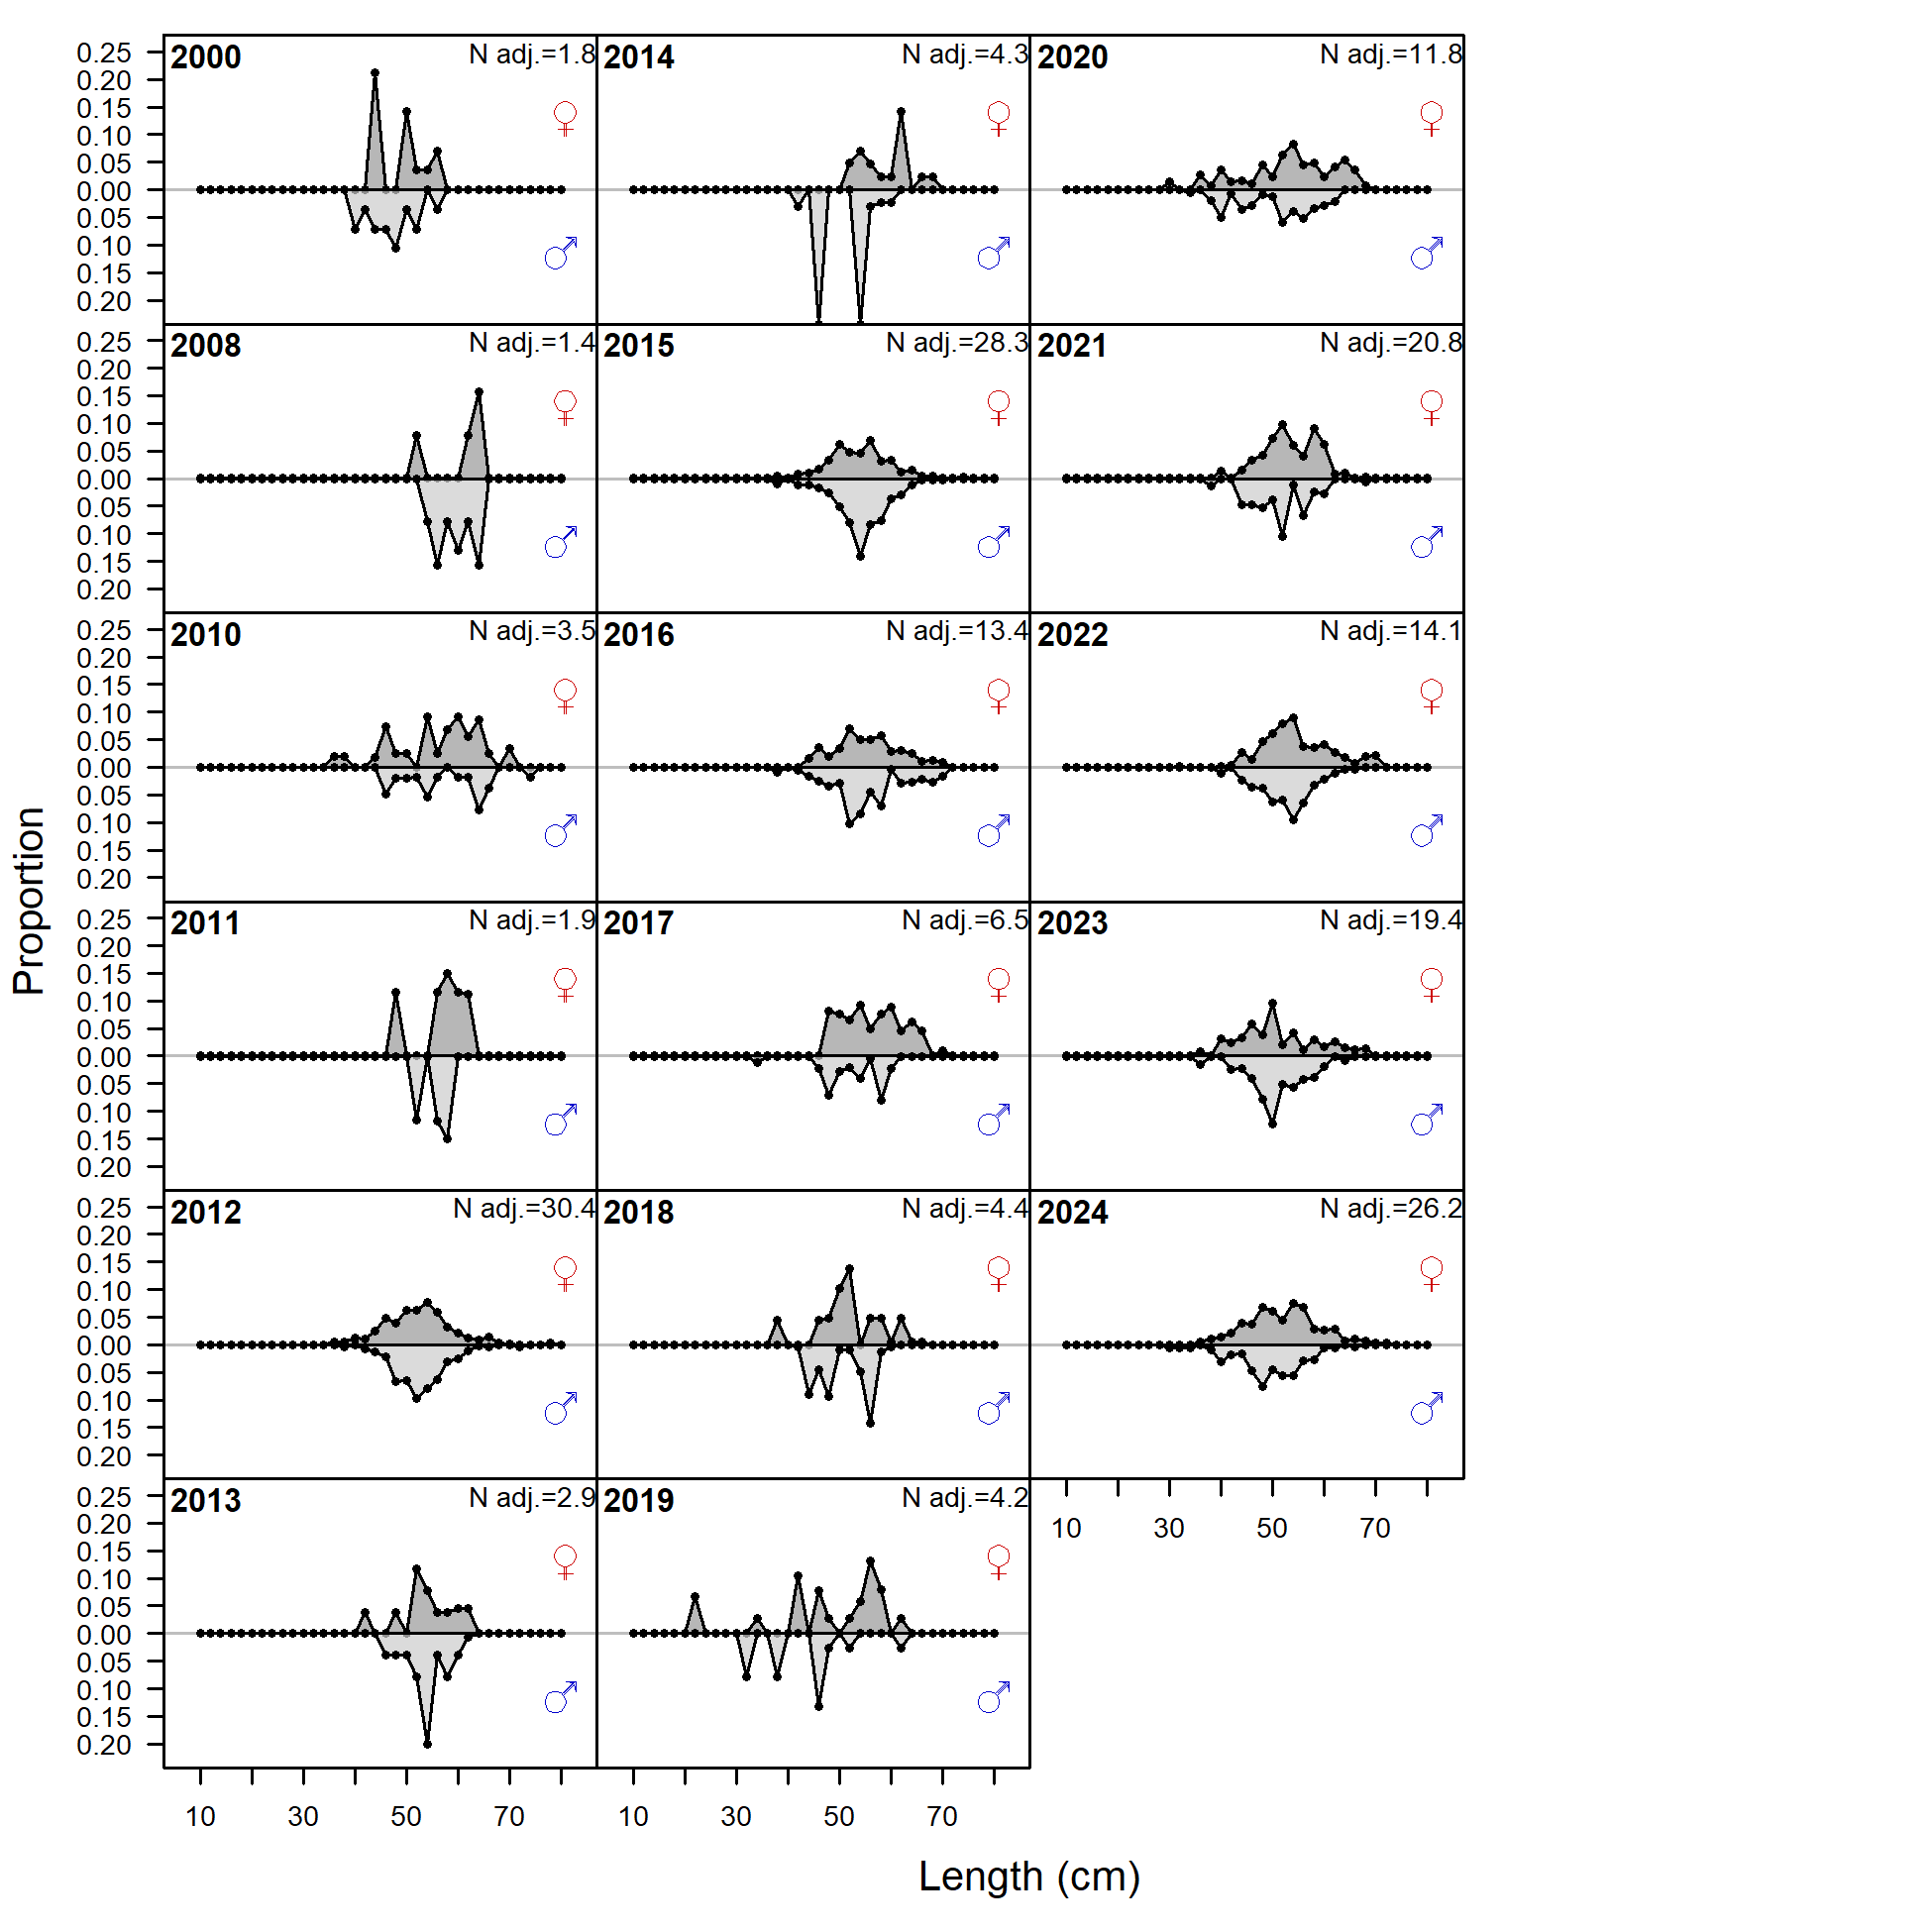
\includegraphics[keepaspectratio]{ref_model/plots/comp_lendat_flt5mkt0.png}}

}

\caption{\label{fig-length_flt5}Length composition data for mid-water
trawl fleet.}

\end{figure}%

\begin{figure}[H]

\centering{

\pandocbounded{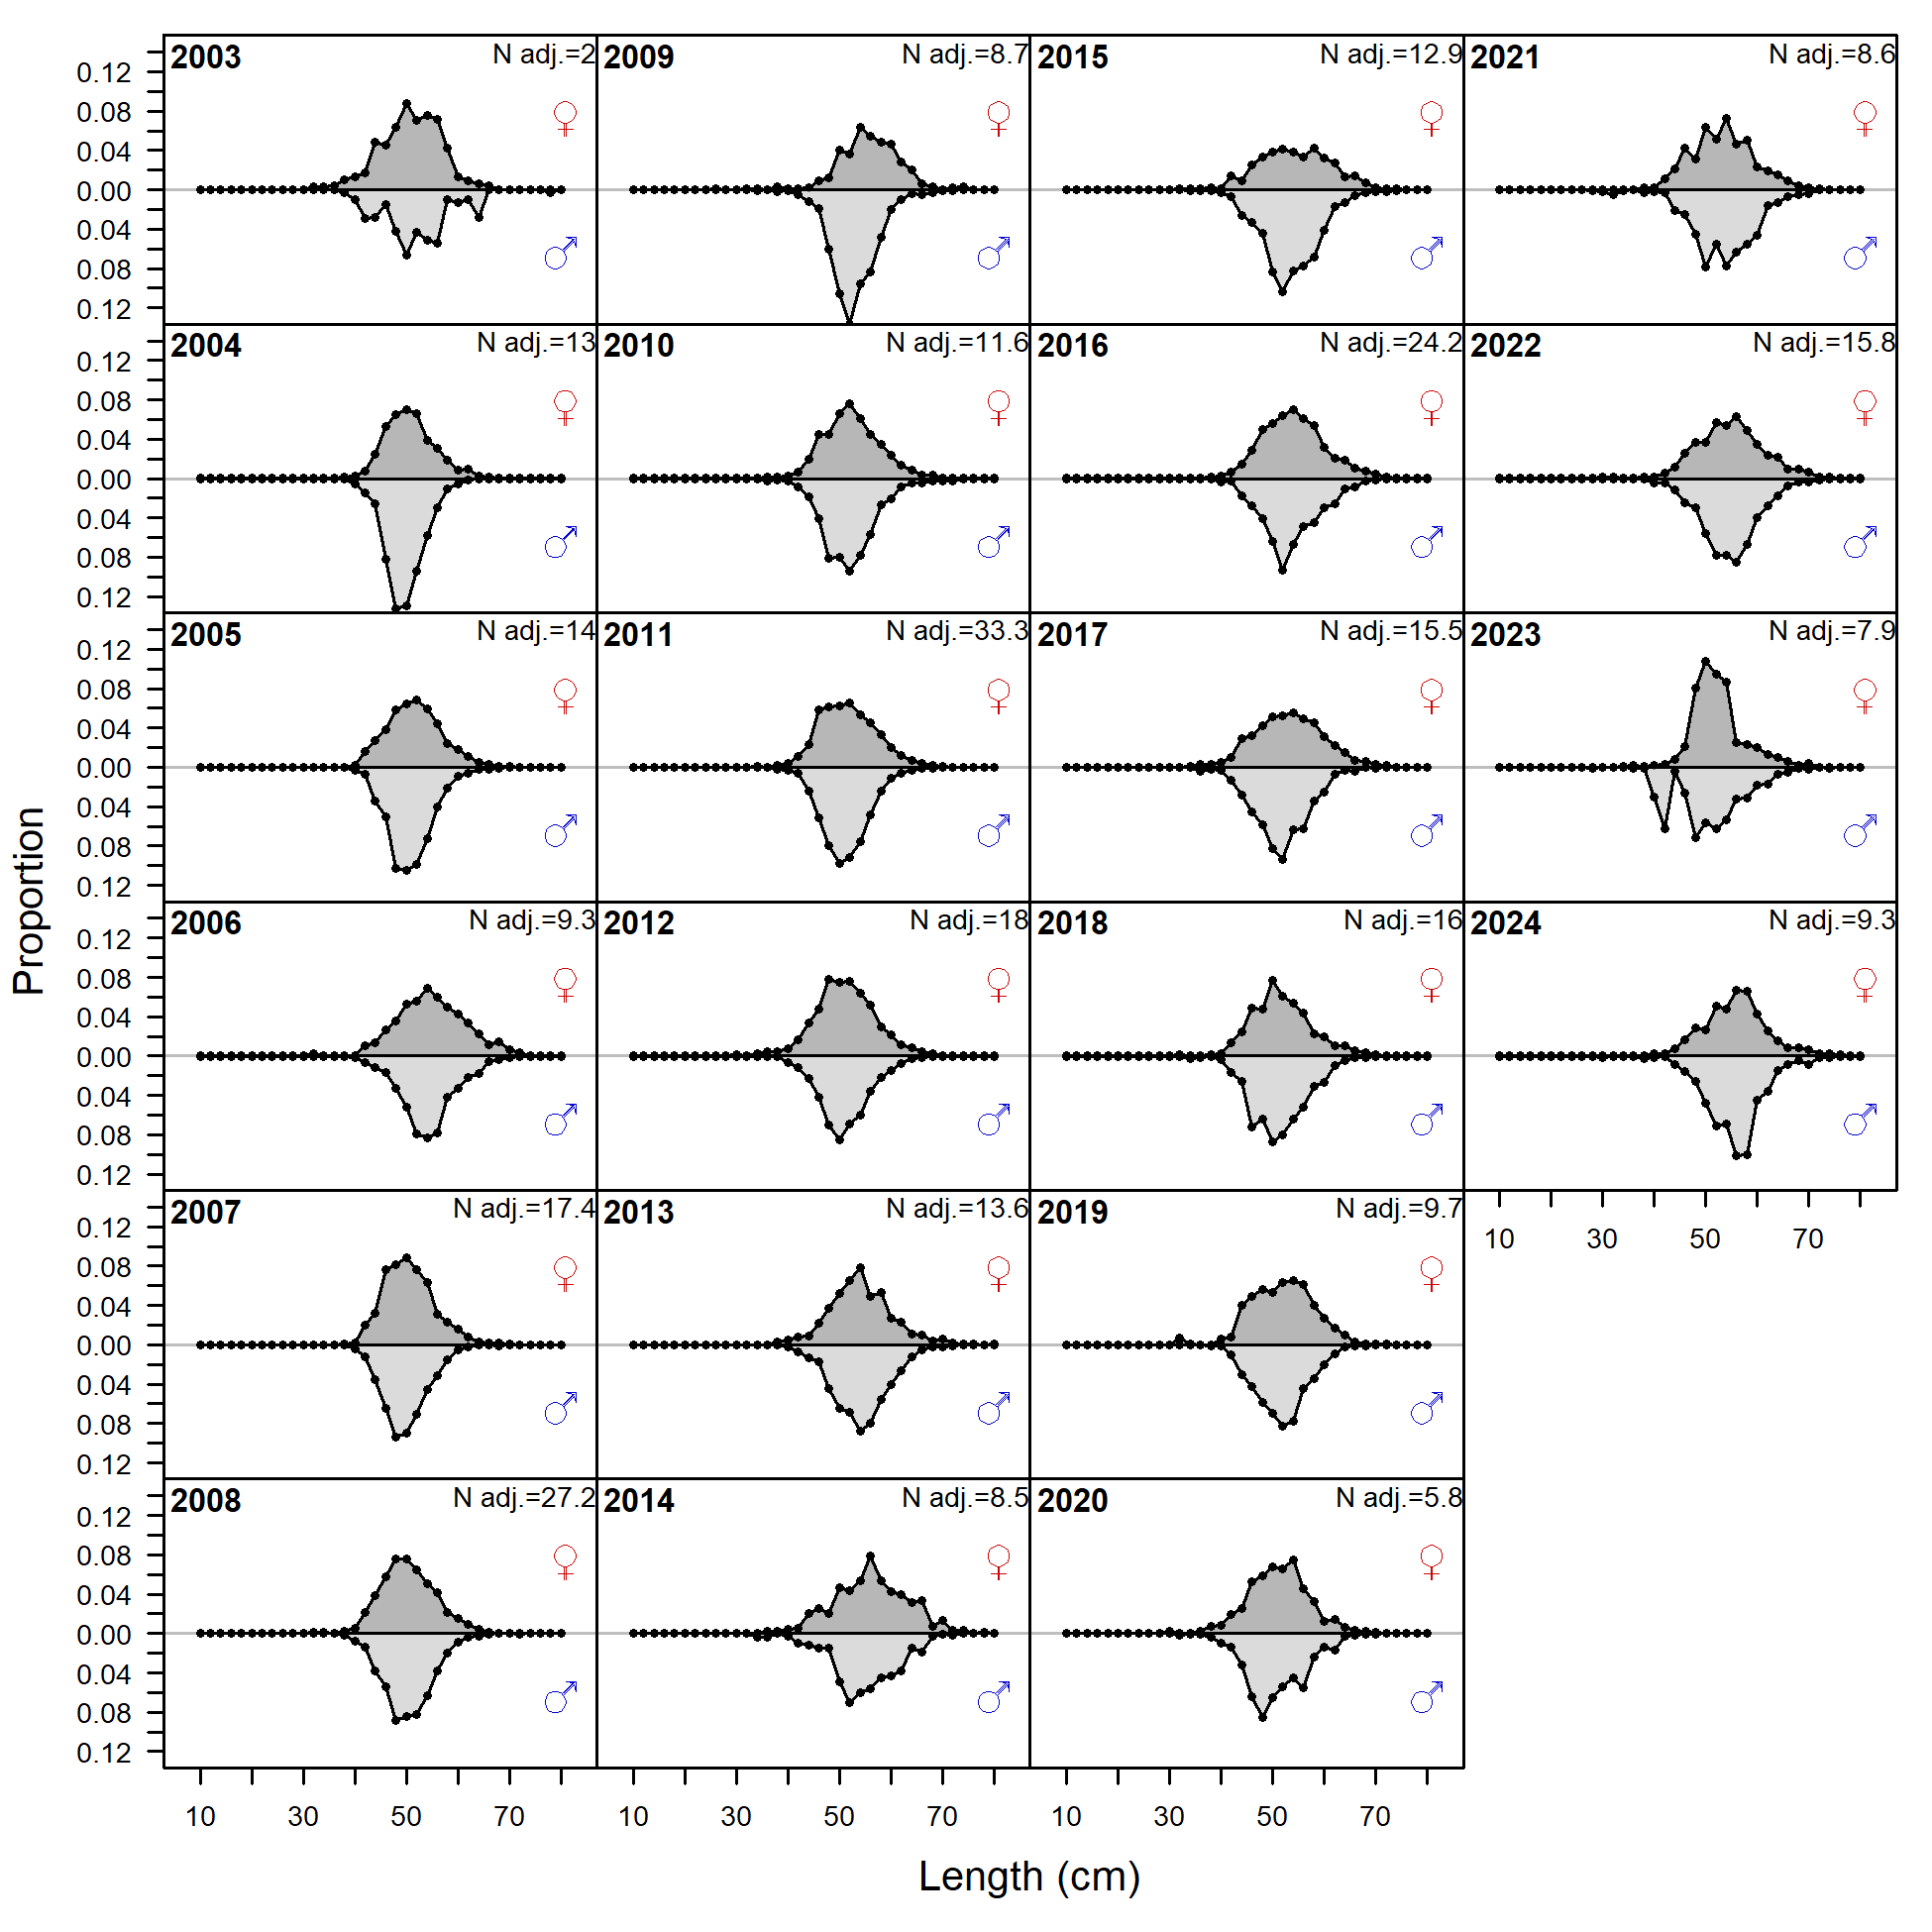
\includegraphics[keepaspectratio]{ref_model/plots/comp_lendat_flt6mkt0.png}}

}

\caption{\label{fig-length_flt6}Length composition data for At-sea Hake
fleet.}

\end{figure}%

\begin{figure}[H]

\centering{

\pandocbounded{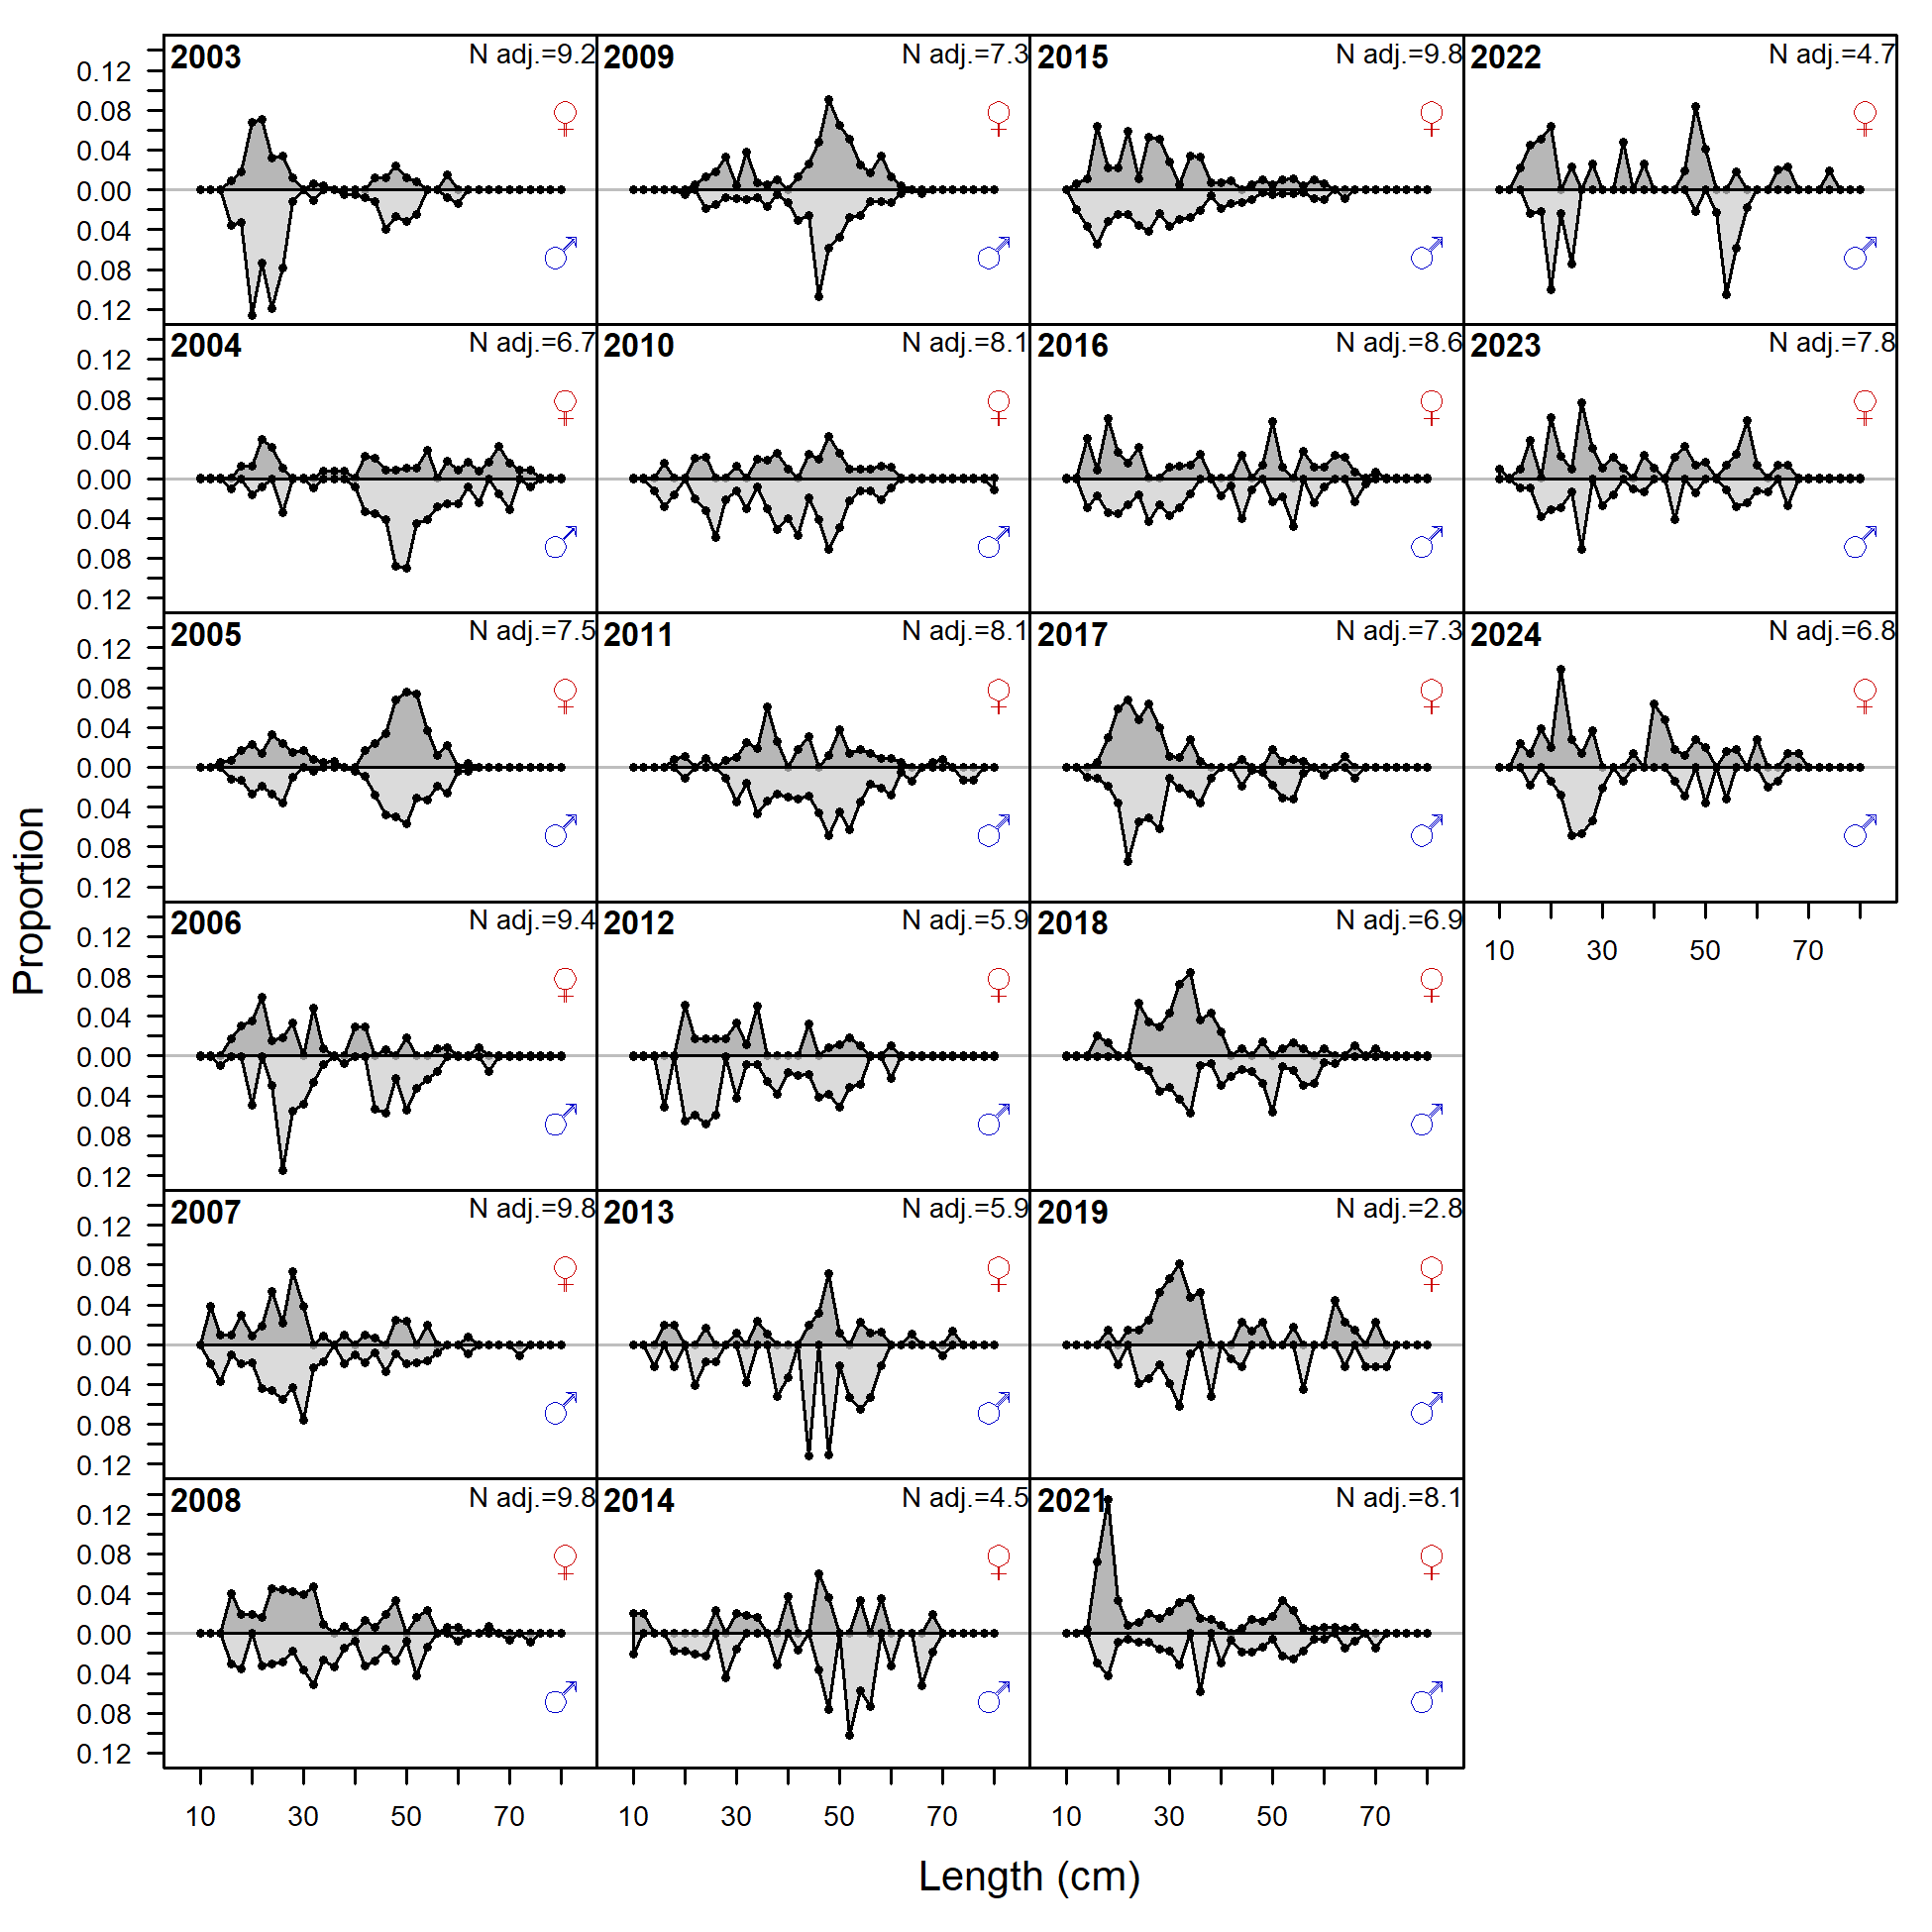
\includegraphics[keepaspectratio]{ref_model/plots/comp_lendat_flt10mkt0.png}}

}

\caption{\label{fig-length_flt10}Length composition data for WCGBTS.}

\end{figure}%

\begin{figure}[H]

\centering{

\pandocbounded{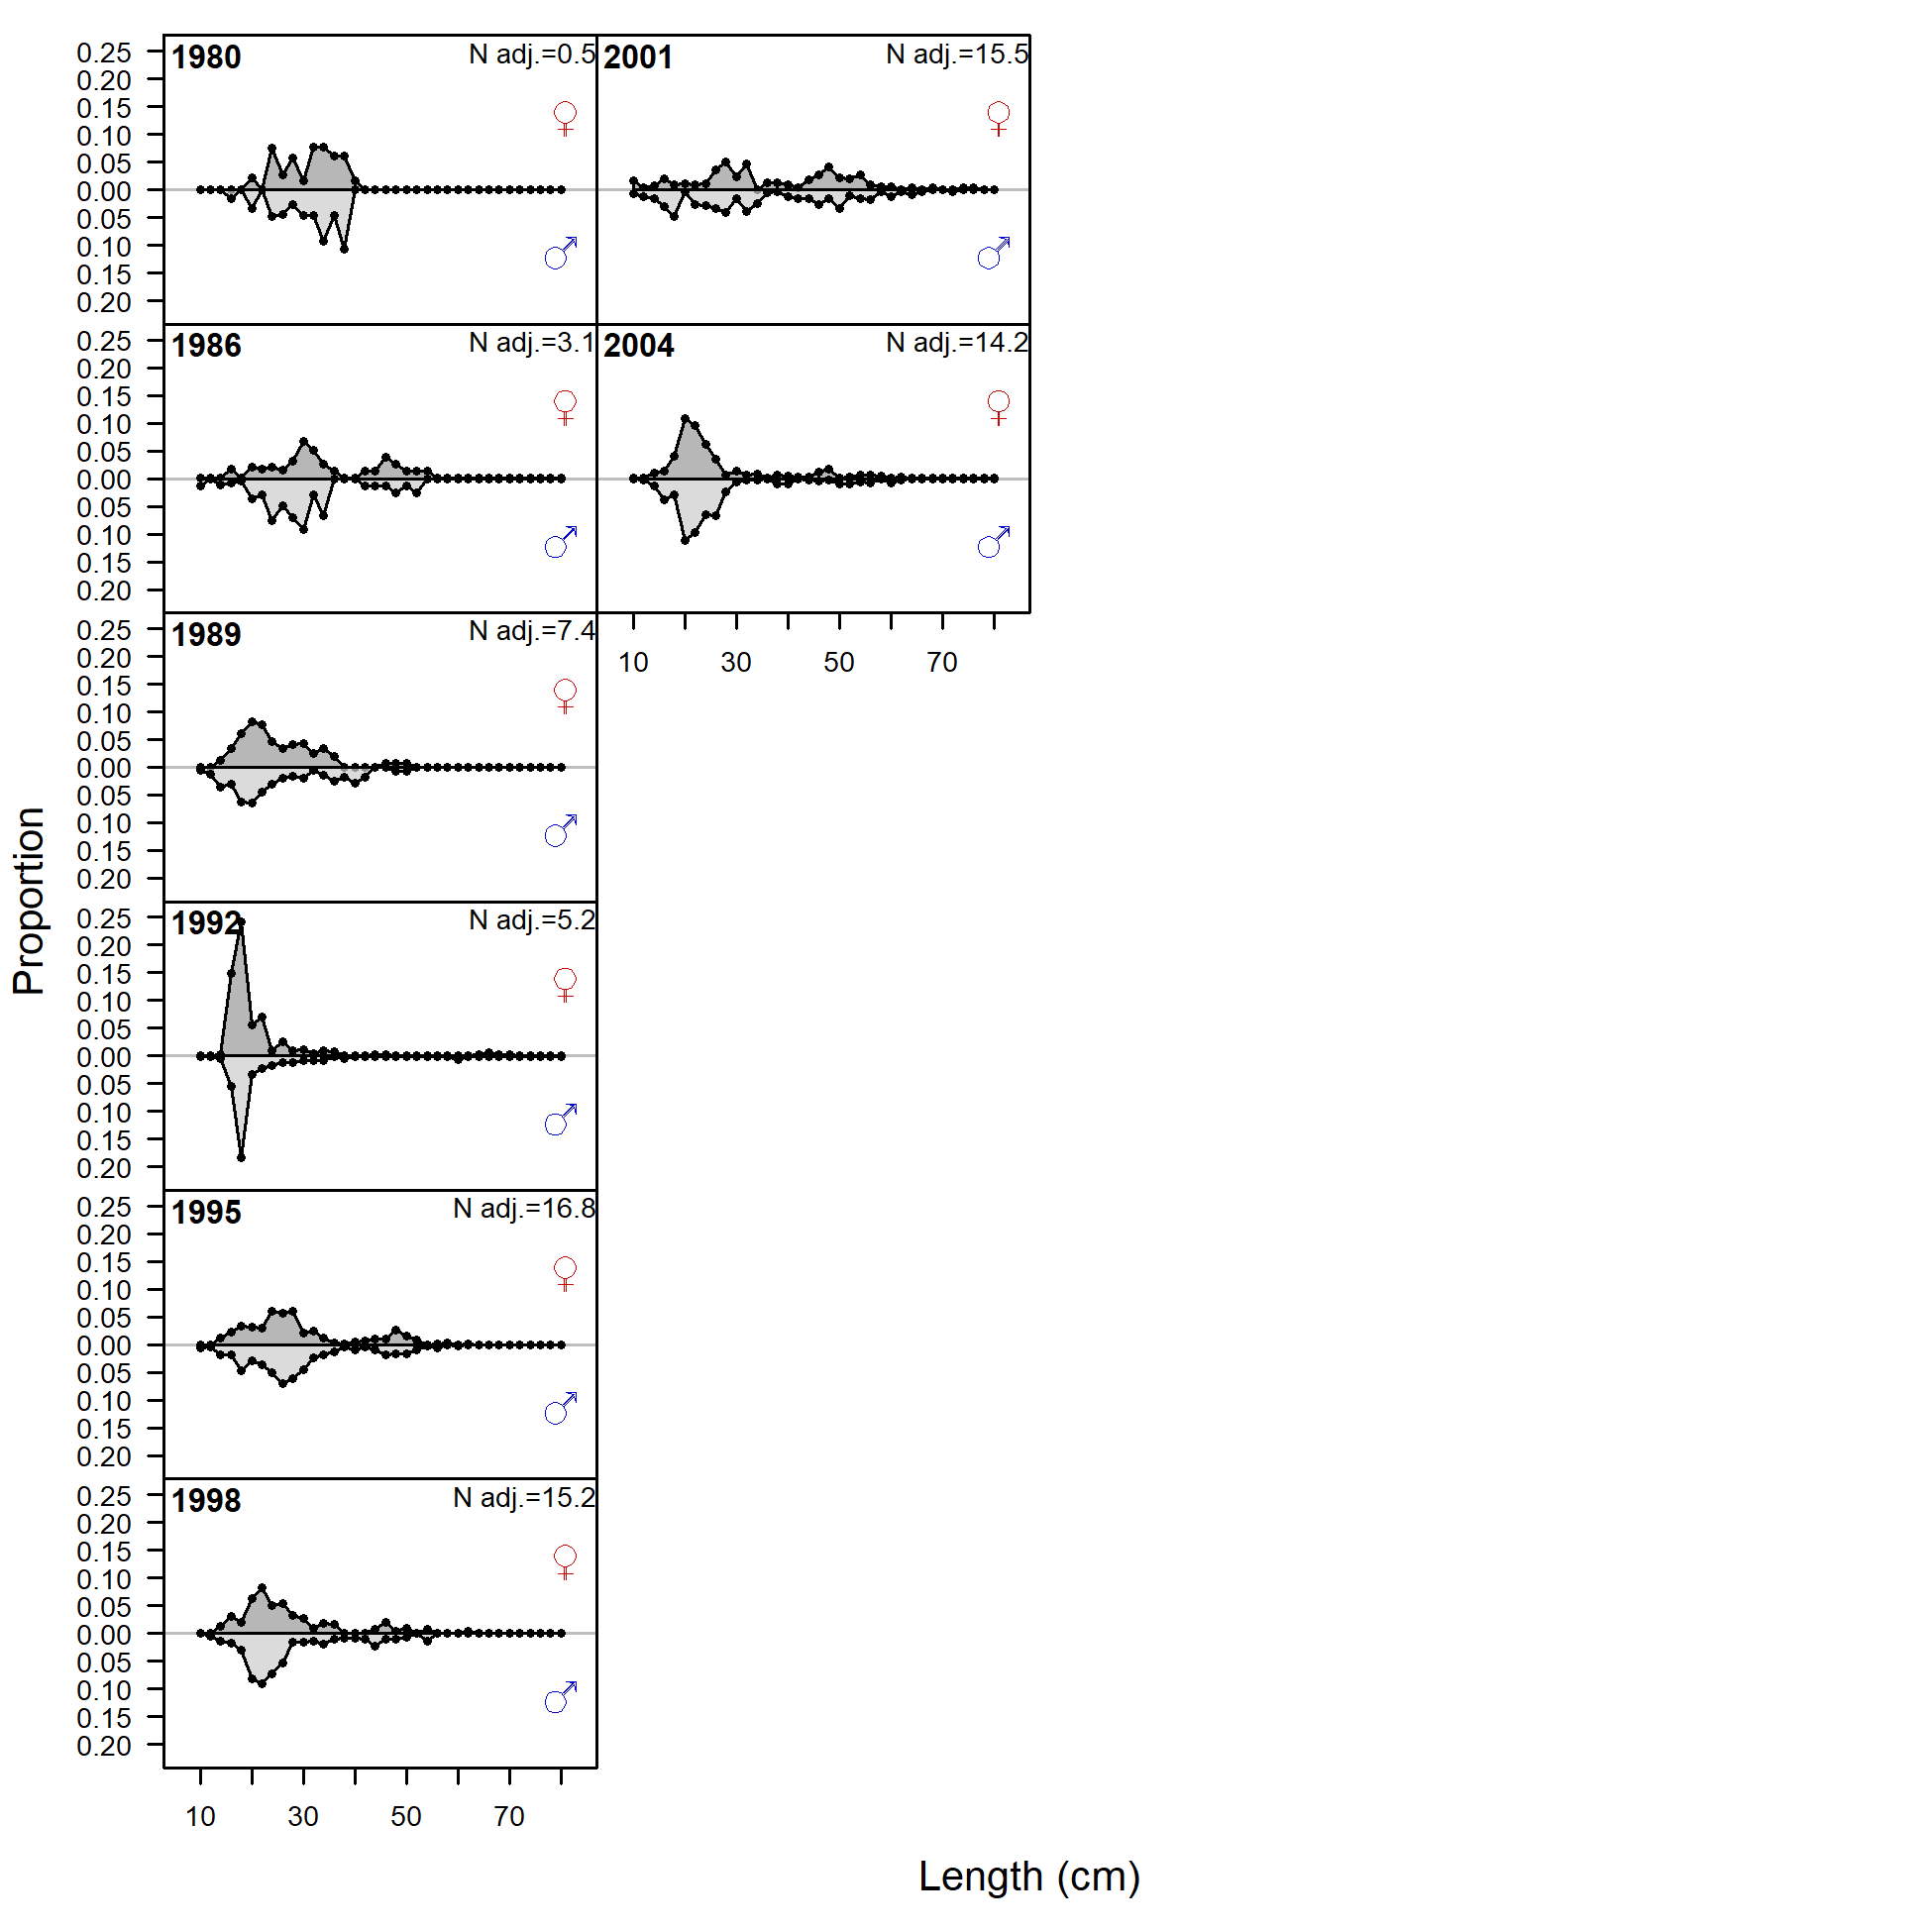
\includegraphics[keepaspectratio]{ref_model/plots/comp_lendat_flt7mkt0.png}}

}

\caption{\label{fig-length_flt7}Length composition data for Triennial
Survey.}

\end{figure}%

\begin{figure}[H]

\centering{

\pandocbounded{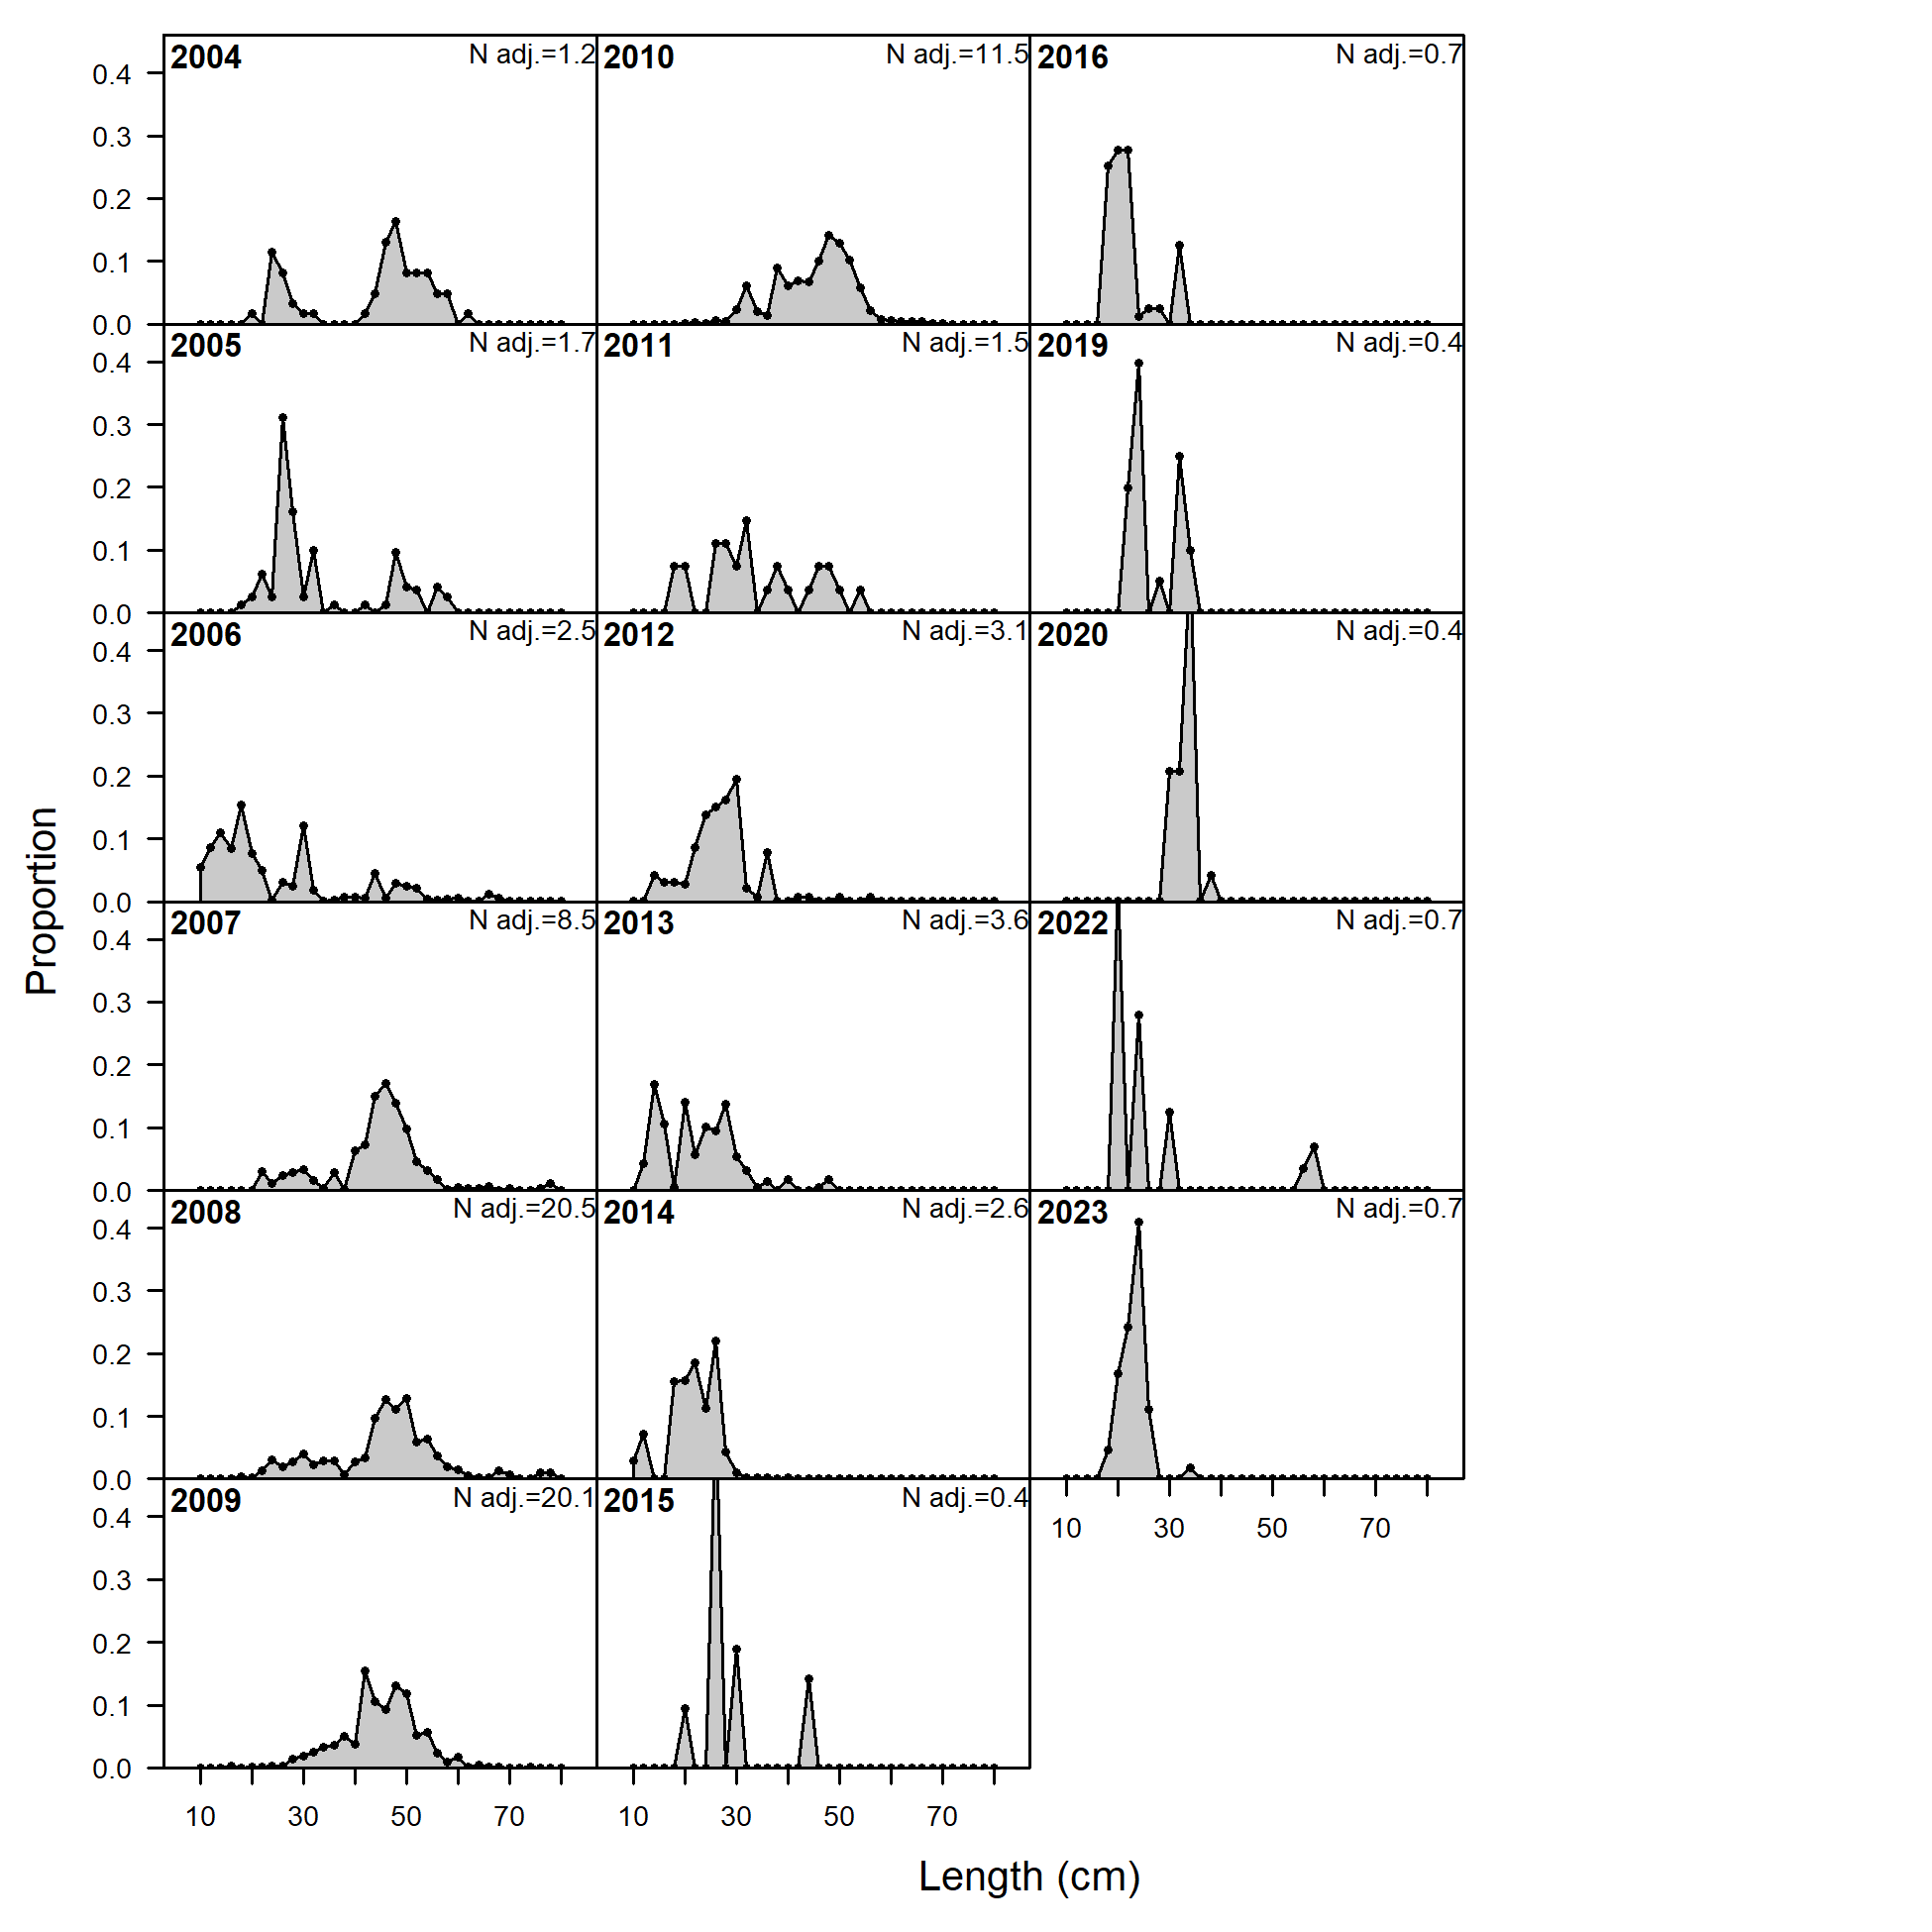
\includegraphics[keepaspectratio]{ref_model/plots/comp_lendat_flt8mkt0.png}}

}

\caption{\label{fig-length_flt8}Length composition data for AFSC Slope
Survey.}

\end{figure}%

\begin{figure}[H]

\centering{

\pandocbounded{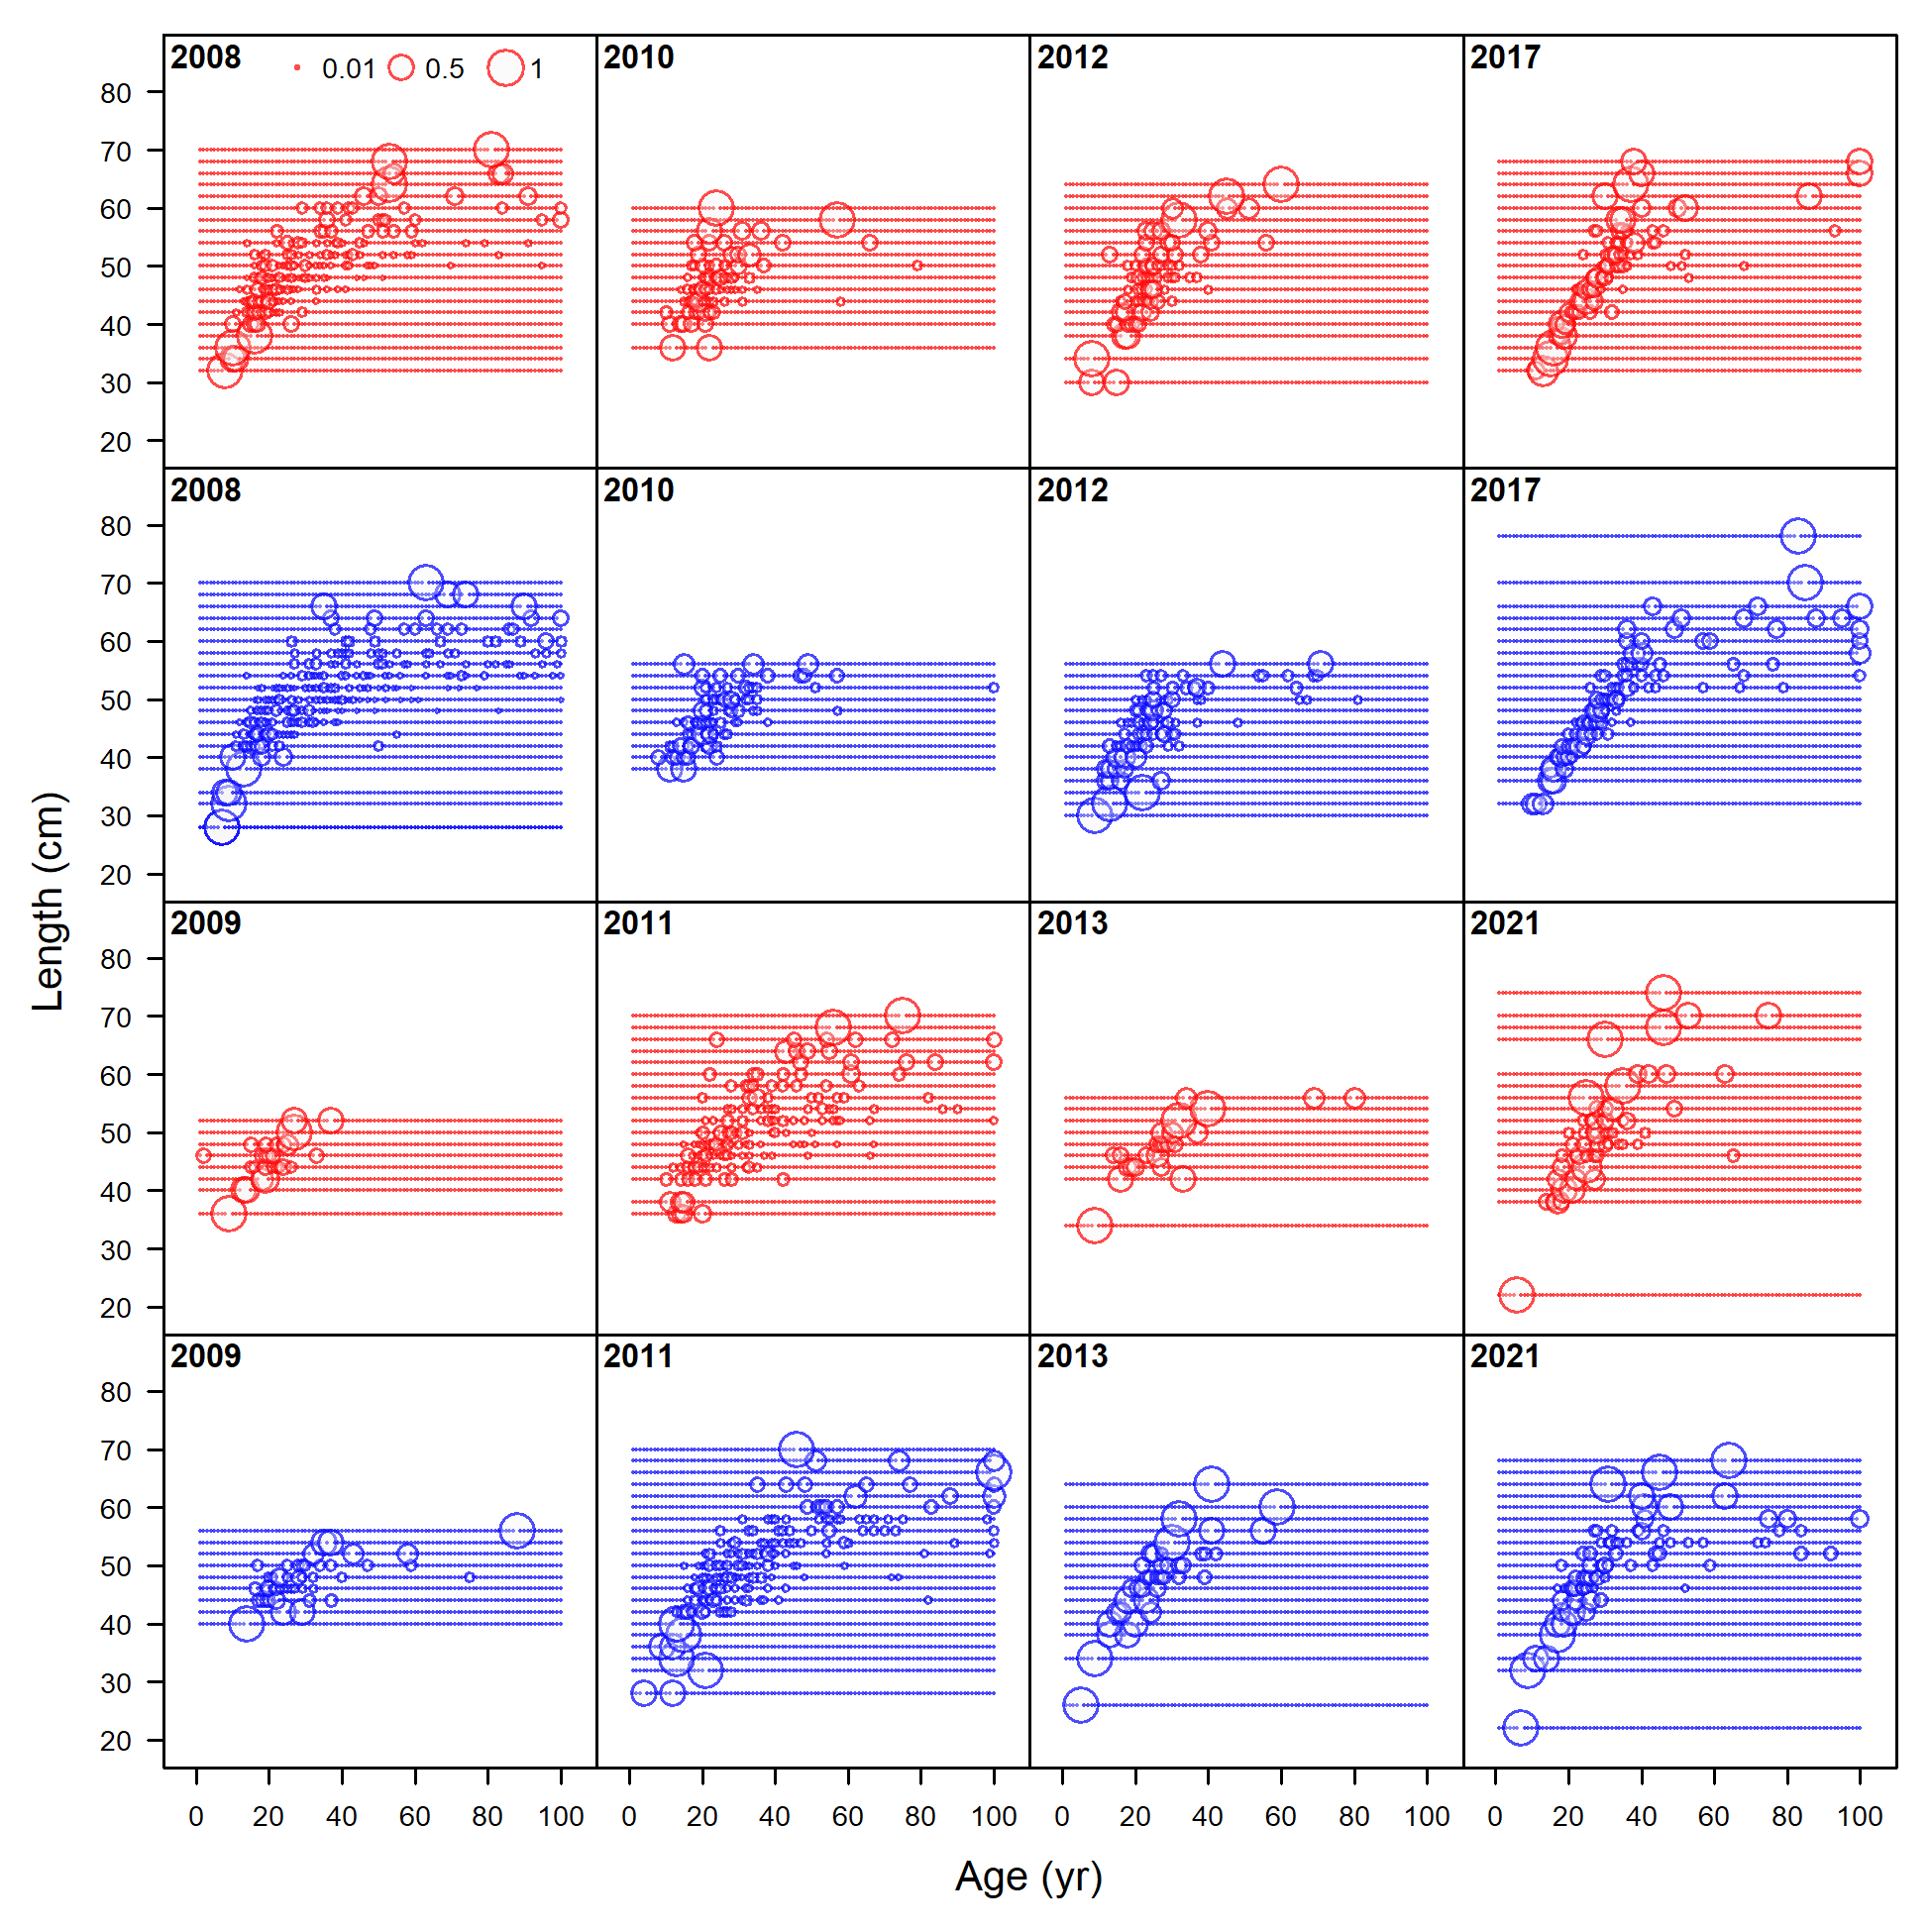
\includegraphics[keepaspectratio]{ref_model/plots/comp_condAALdat_bubflt1mkt0_page1.png}}

}

\caption{\label{fig-caal_flt1_1}Length composition data for bottom trawl
fleet.}

\end{figure}%

\begin{figure}[H]

\centering{

\pandocbounded{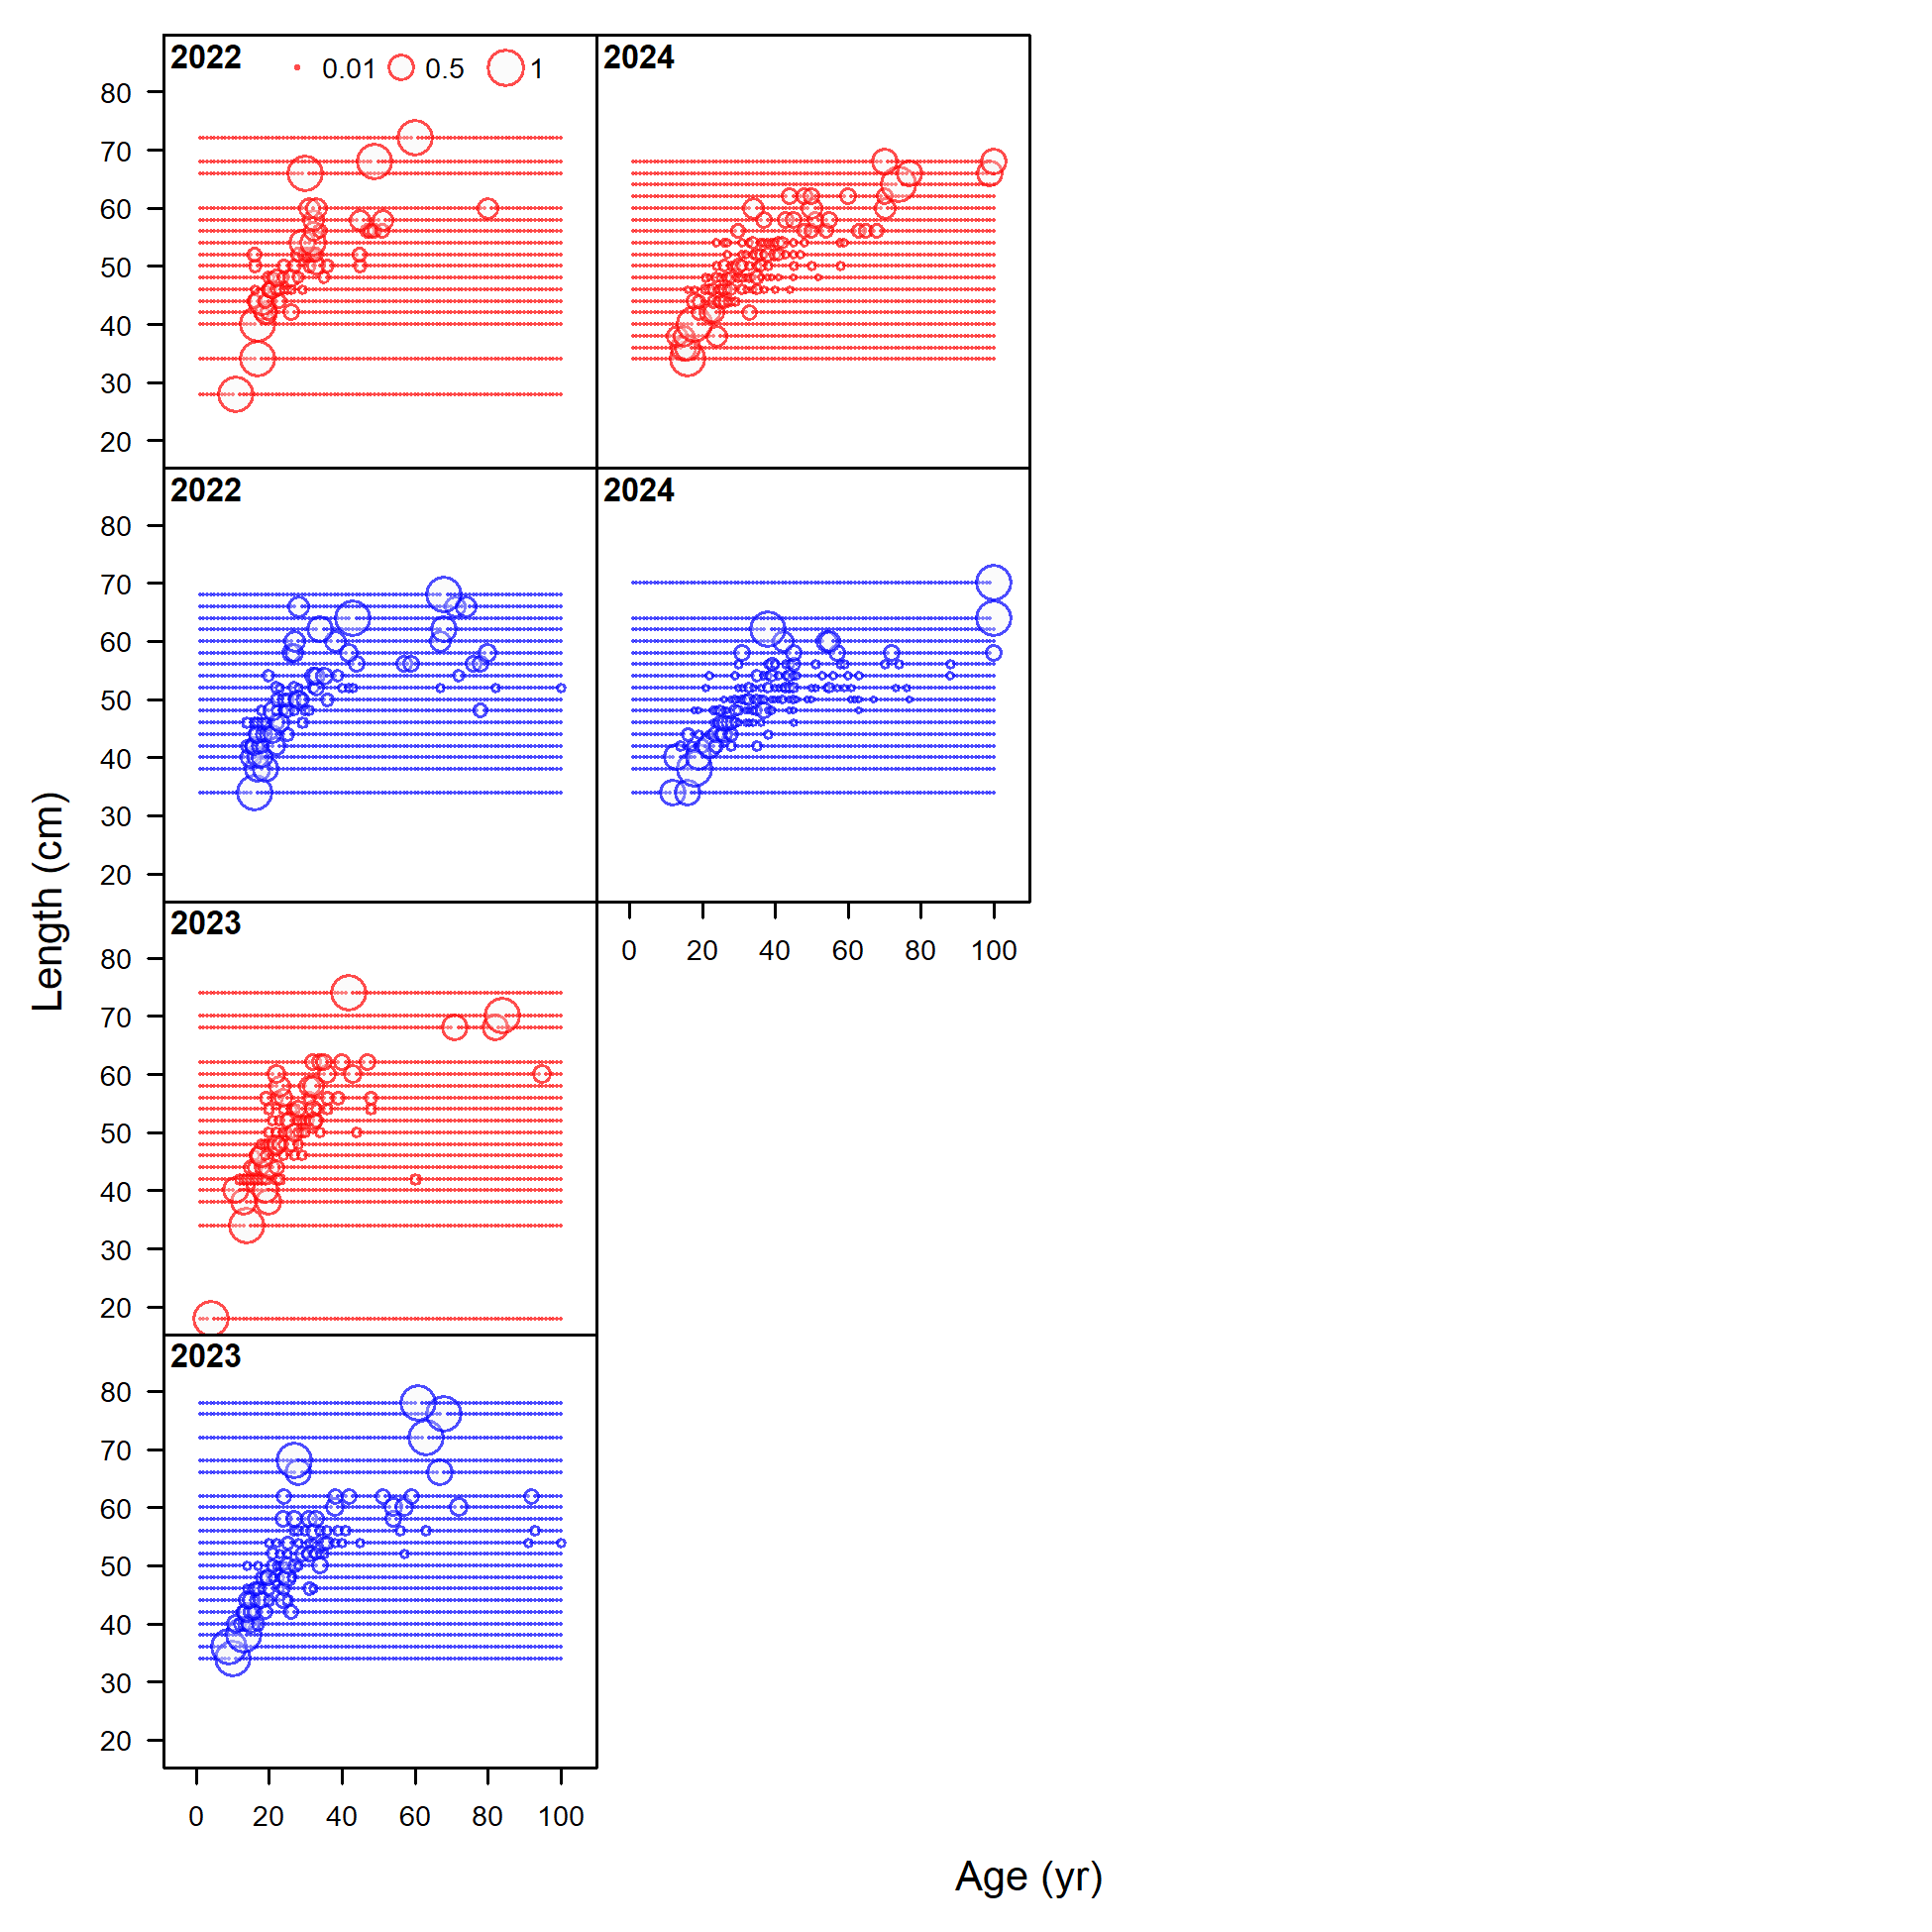
\includegraphics[keepaspectratio]{ref_model/plots/comp_condAALdat_bubflt1mkt0_page2.png}}

}

\caption{\label{fig-caal_flt1_2}Length composition data for bottom trawl
fleet, continued.}

\end{figure}%

\begin{figure}[H]

\centering{

\pandocbounded{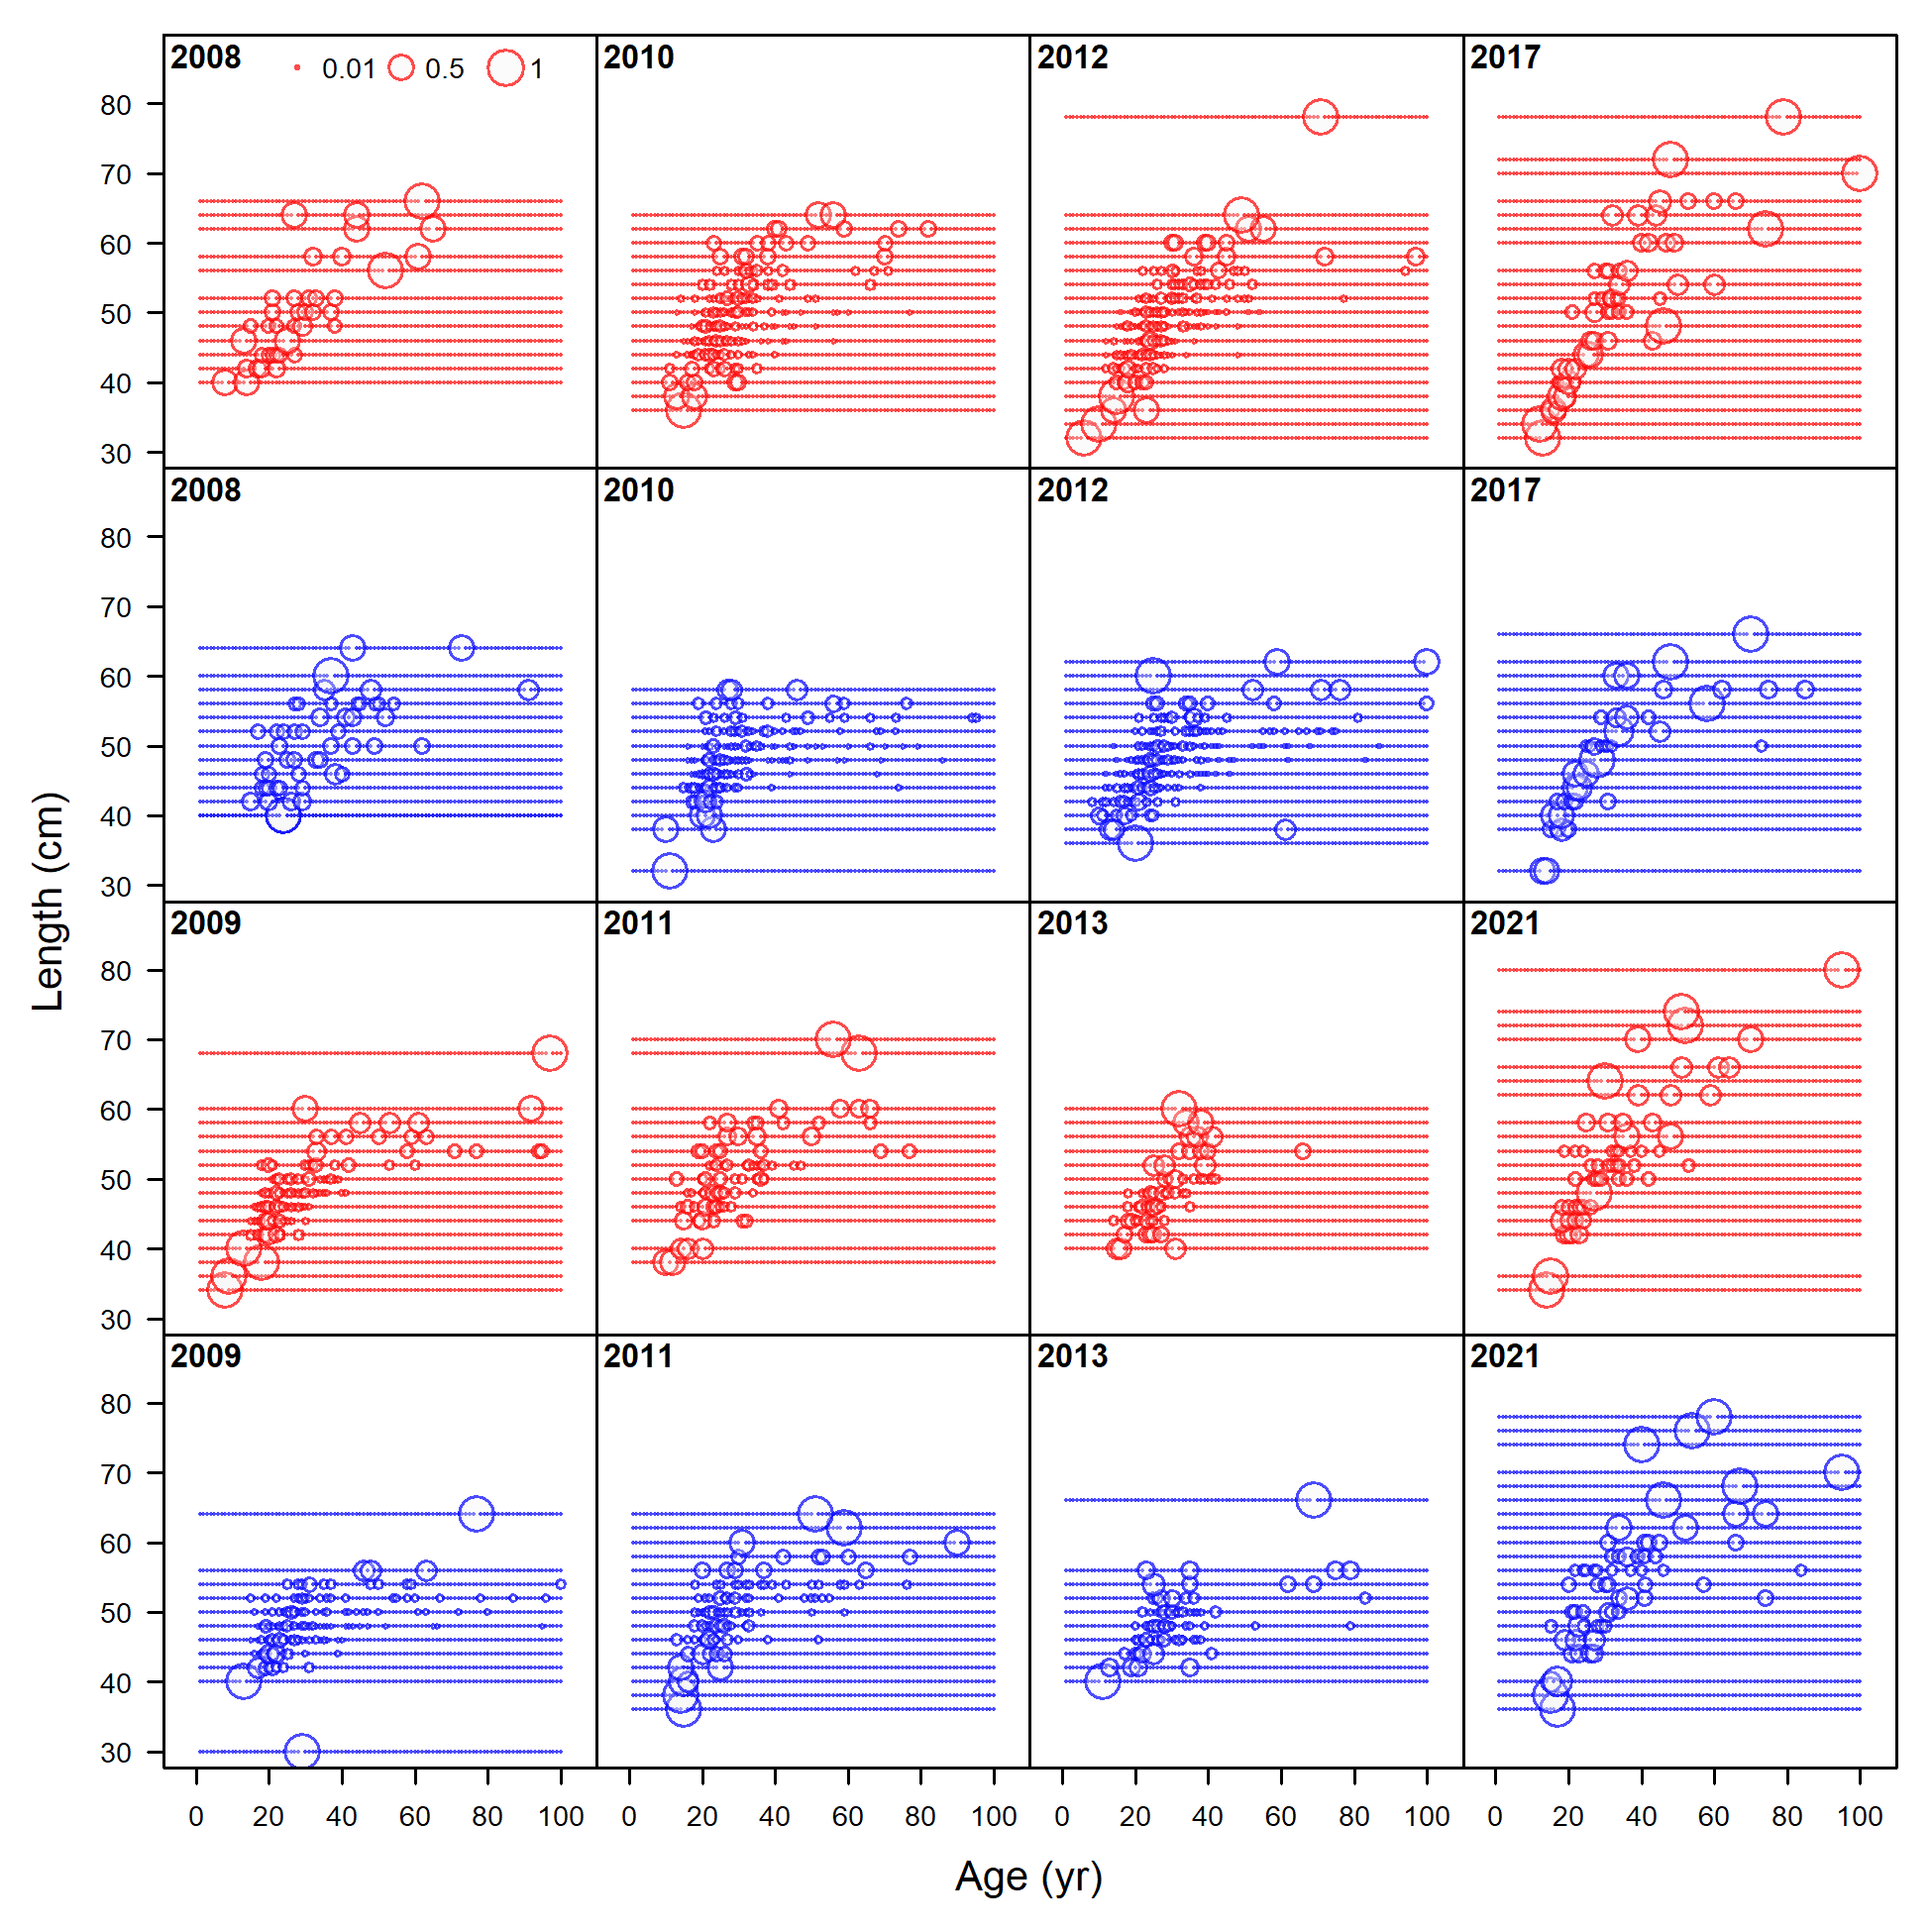
\includegraphics[keepaspectratio]{ref_model/plots/comp_condAALdat_bubflt3mkt0_page1.png}}

}

\caption{\label{fig-caal_flt3_1}Conditional ages-at-length composition
data for non-trawl fleet.}

\end{figure}%

\begin{figure}[H]

\centering{

\pandocbounded{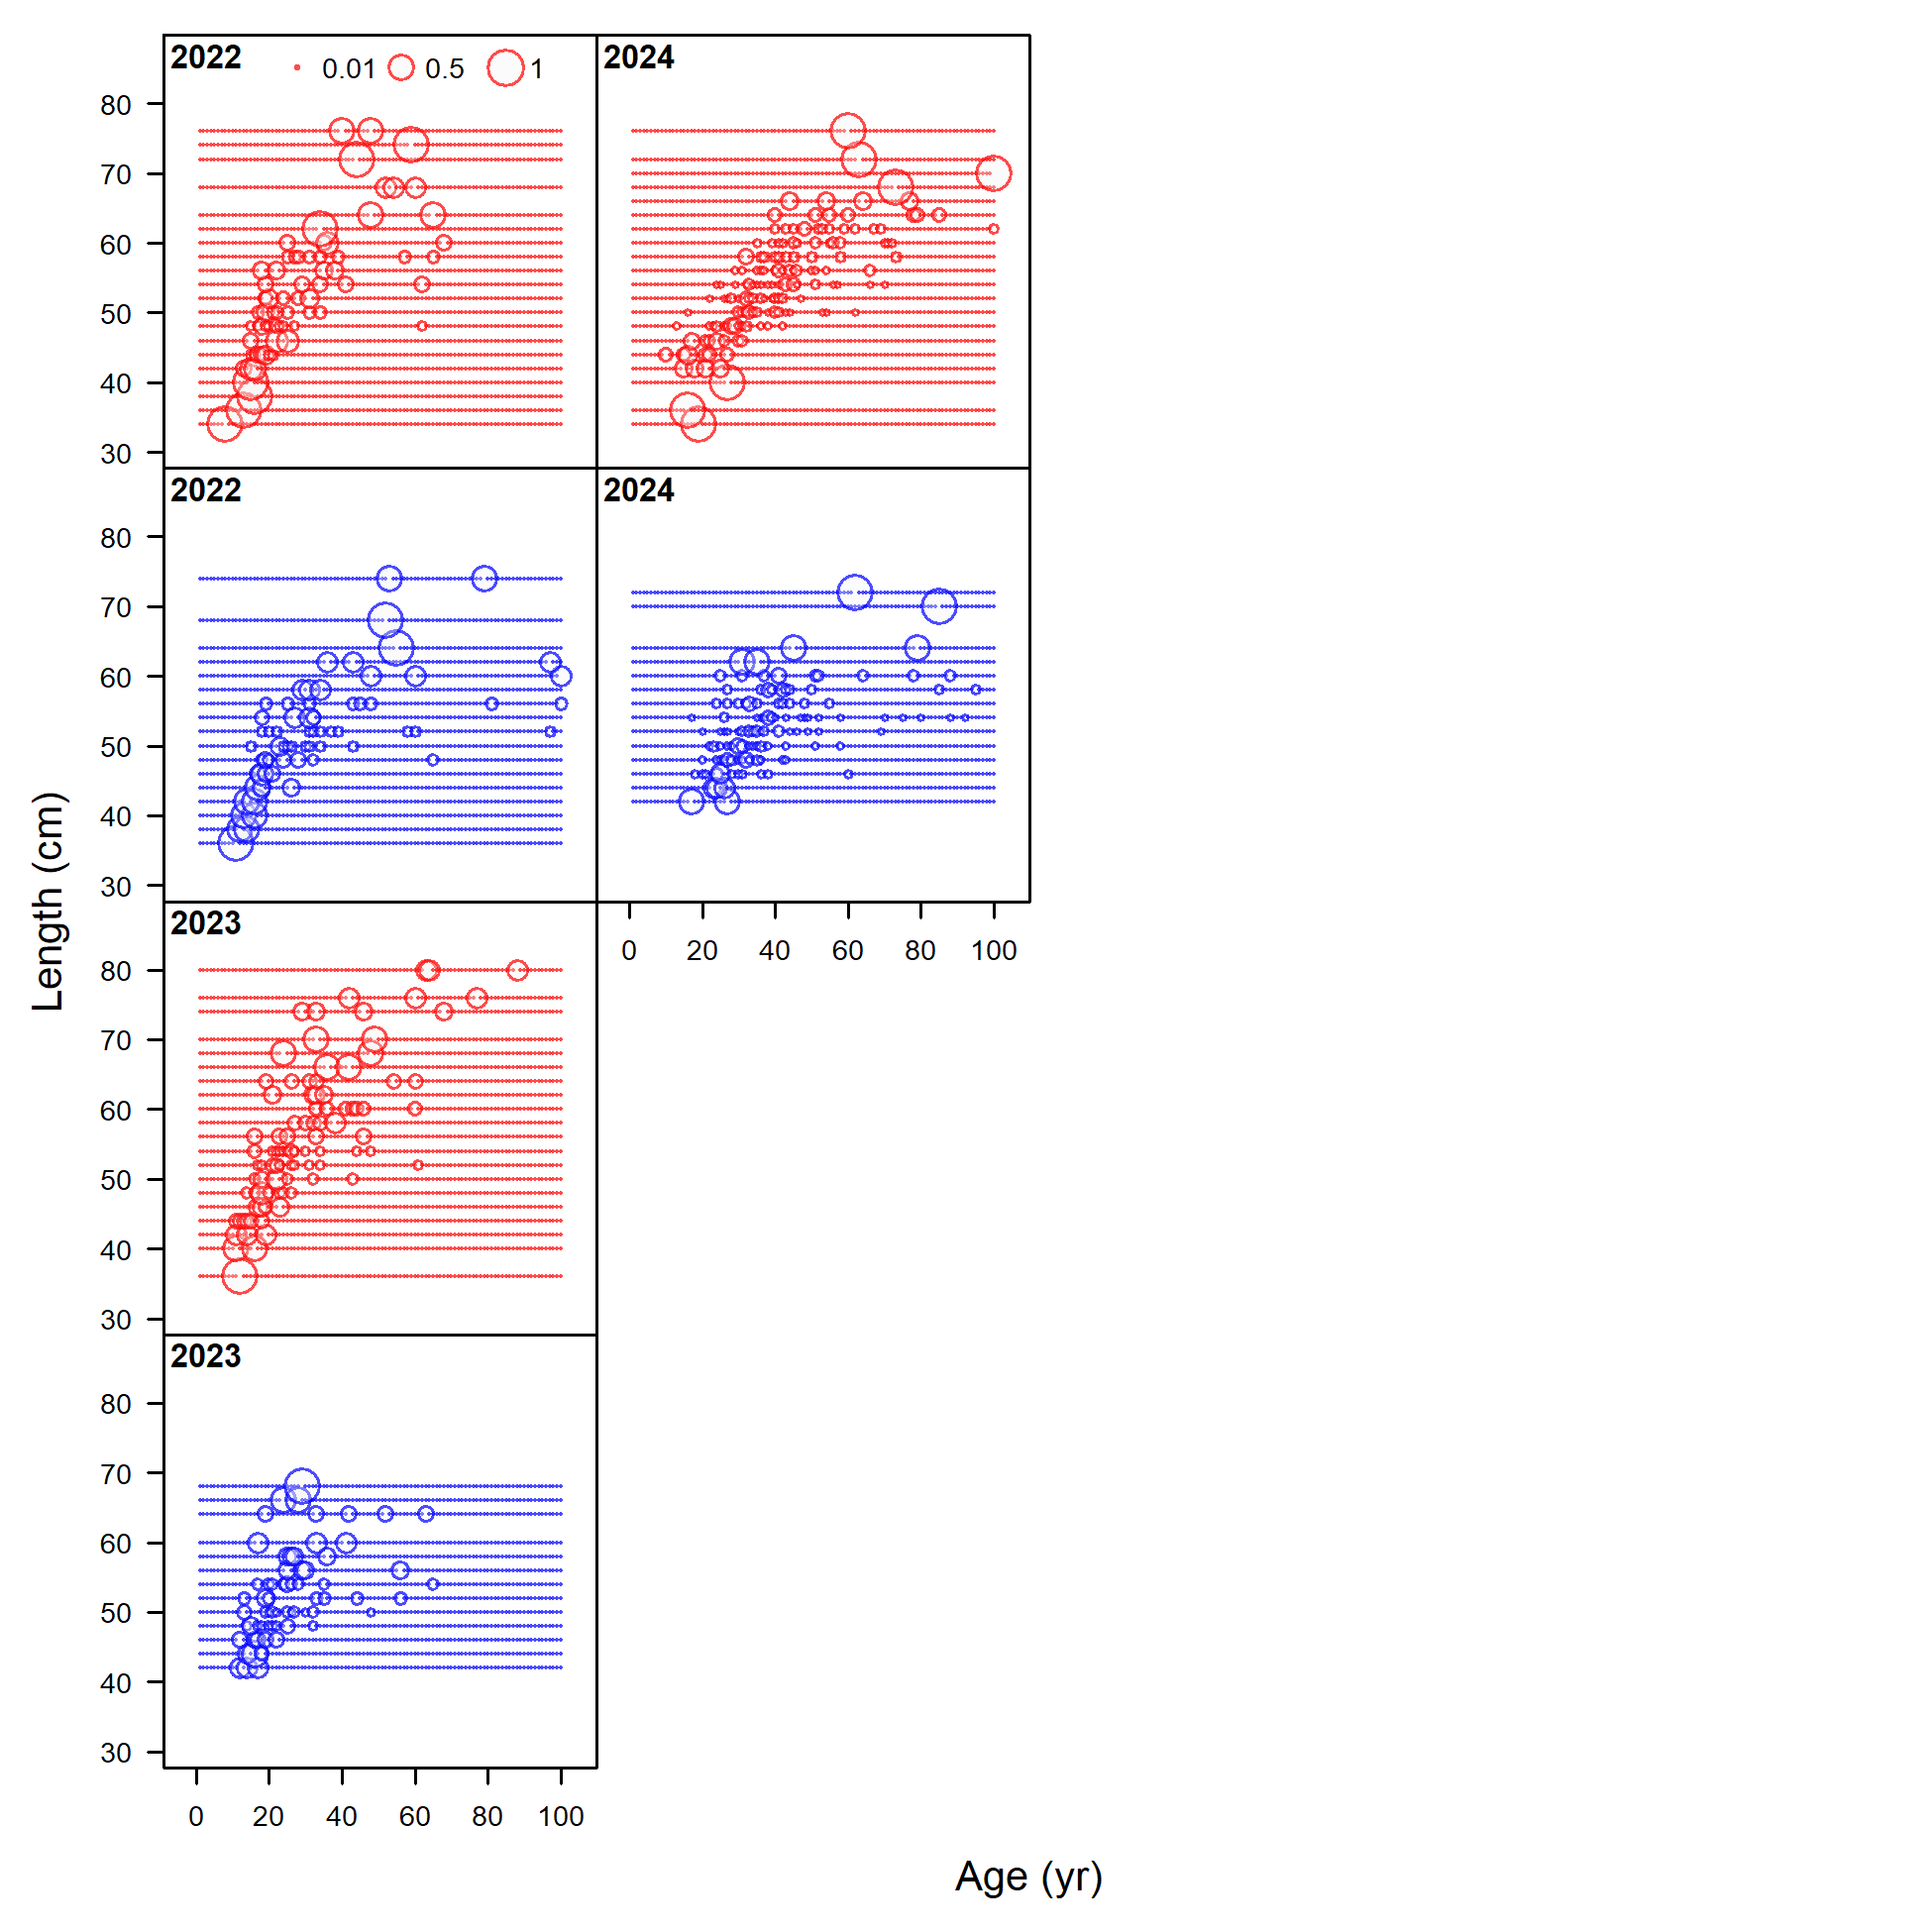
\includegraphics[keepaspectratio]{ref_model/plots/comp_condAALdat_bubflt3mkt0_page2.png}}

}

\caption{\label{fig-caal_flt3_2}Conditional ages-at-length composition
data for non-trawl fleet, continued.}

\end{figure}%

\begin{figure}[H]

\centering{

\pandocbounded{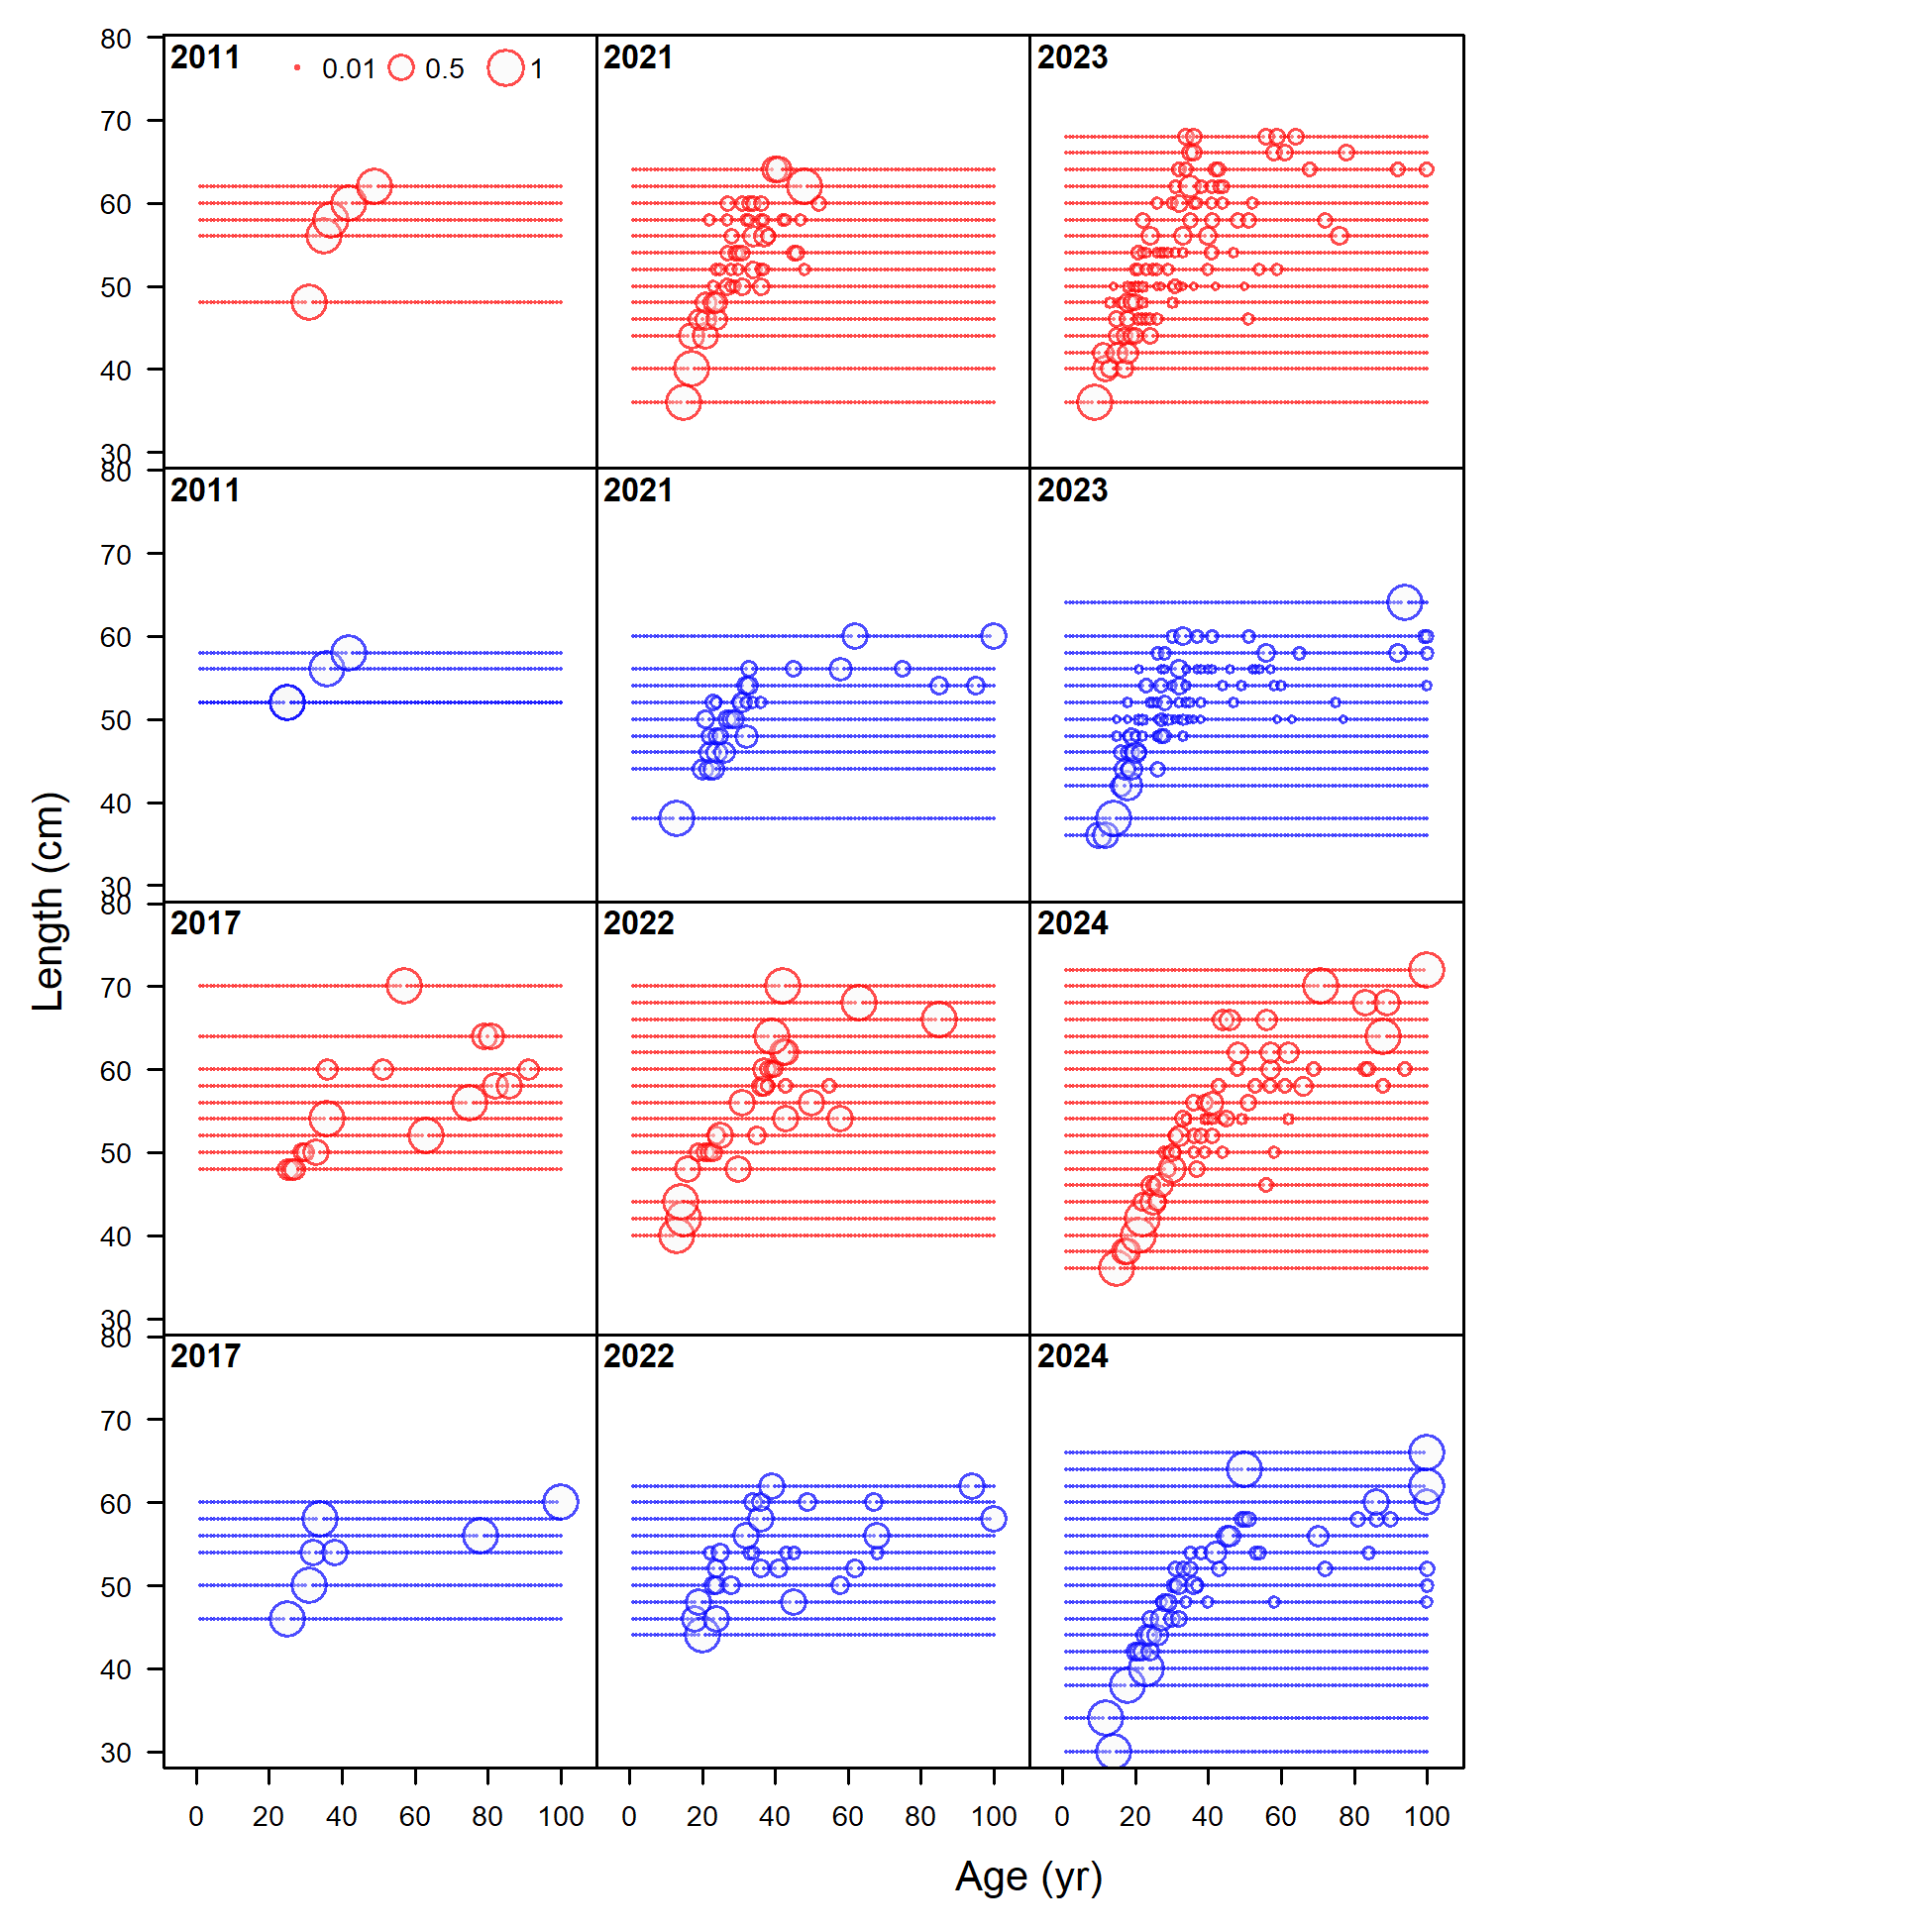
\includegraphics[keepaspectratio]{ref_model/plots/comp_condAALdat_bubflt5mkt0.png}}

}

\caption{\label{fig-caal_flt5}Conditional ages-at-length composition
data for Midwater trawl fleet.}

\end{figure}%

\begin{figure}[H]

\centering{

\pandocbounded{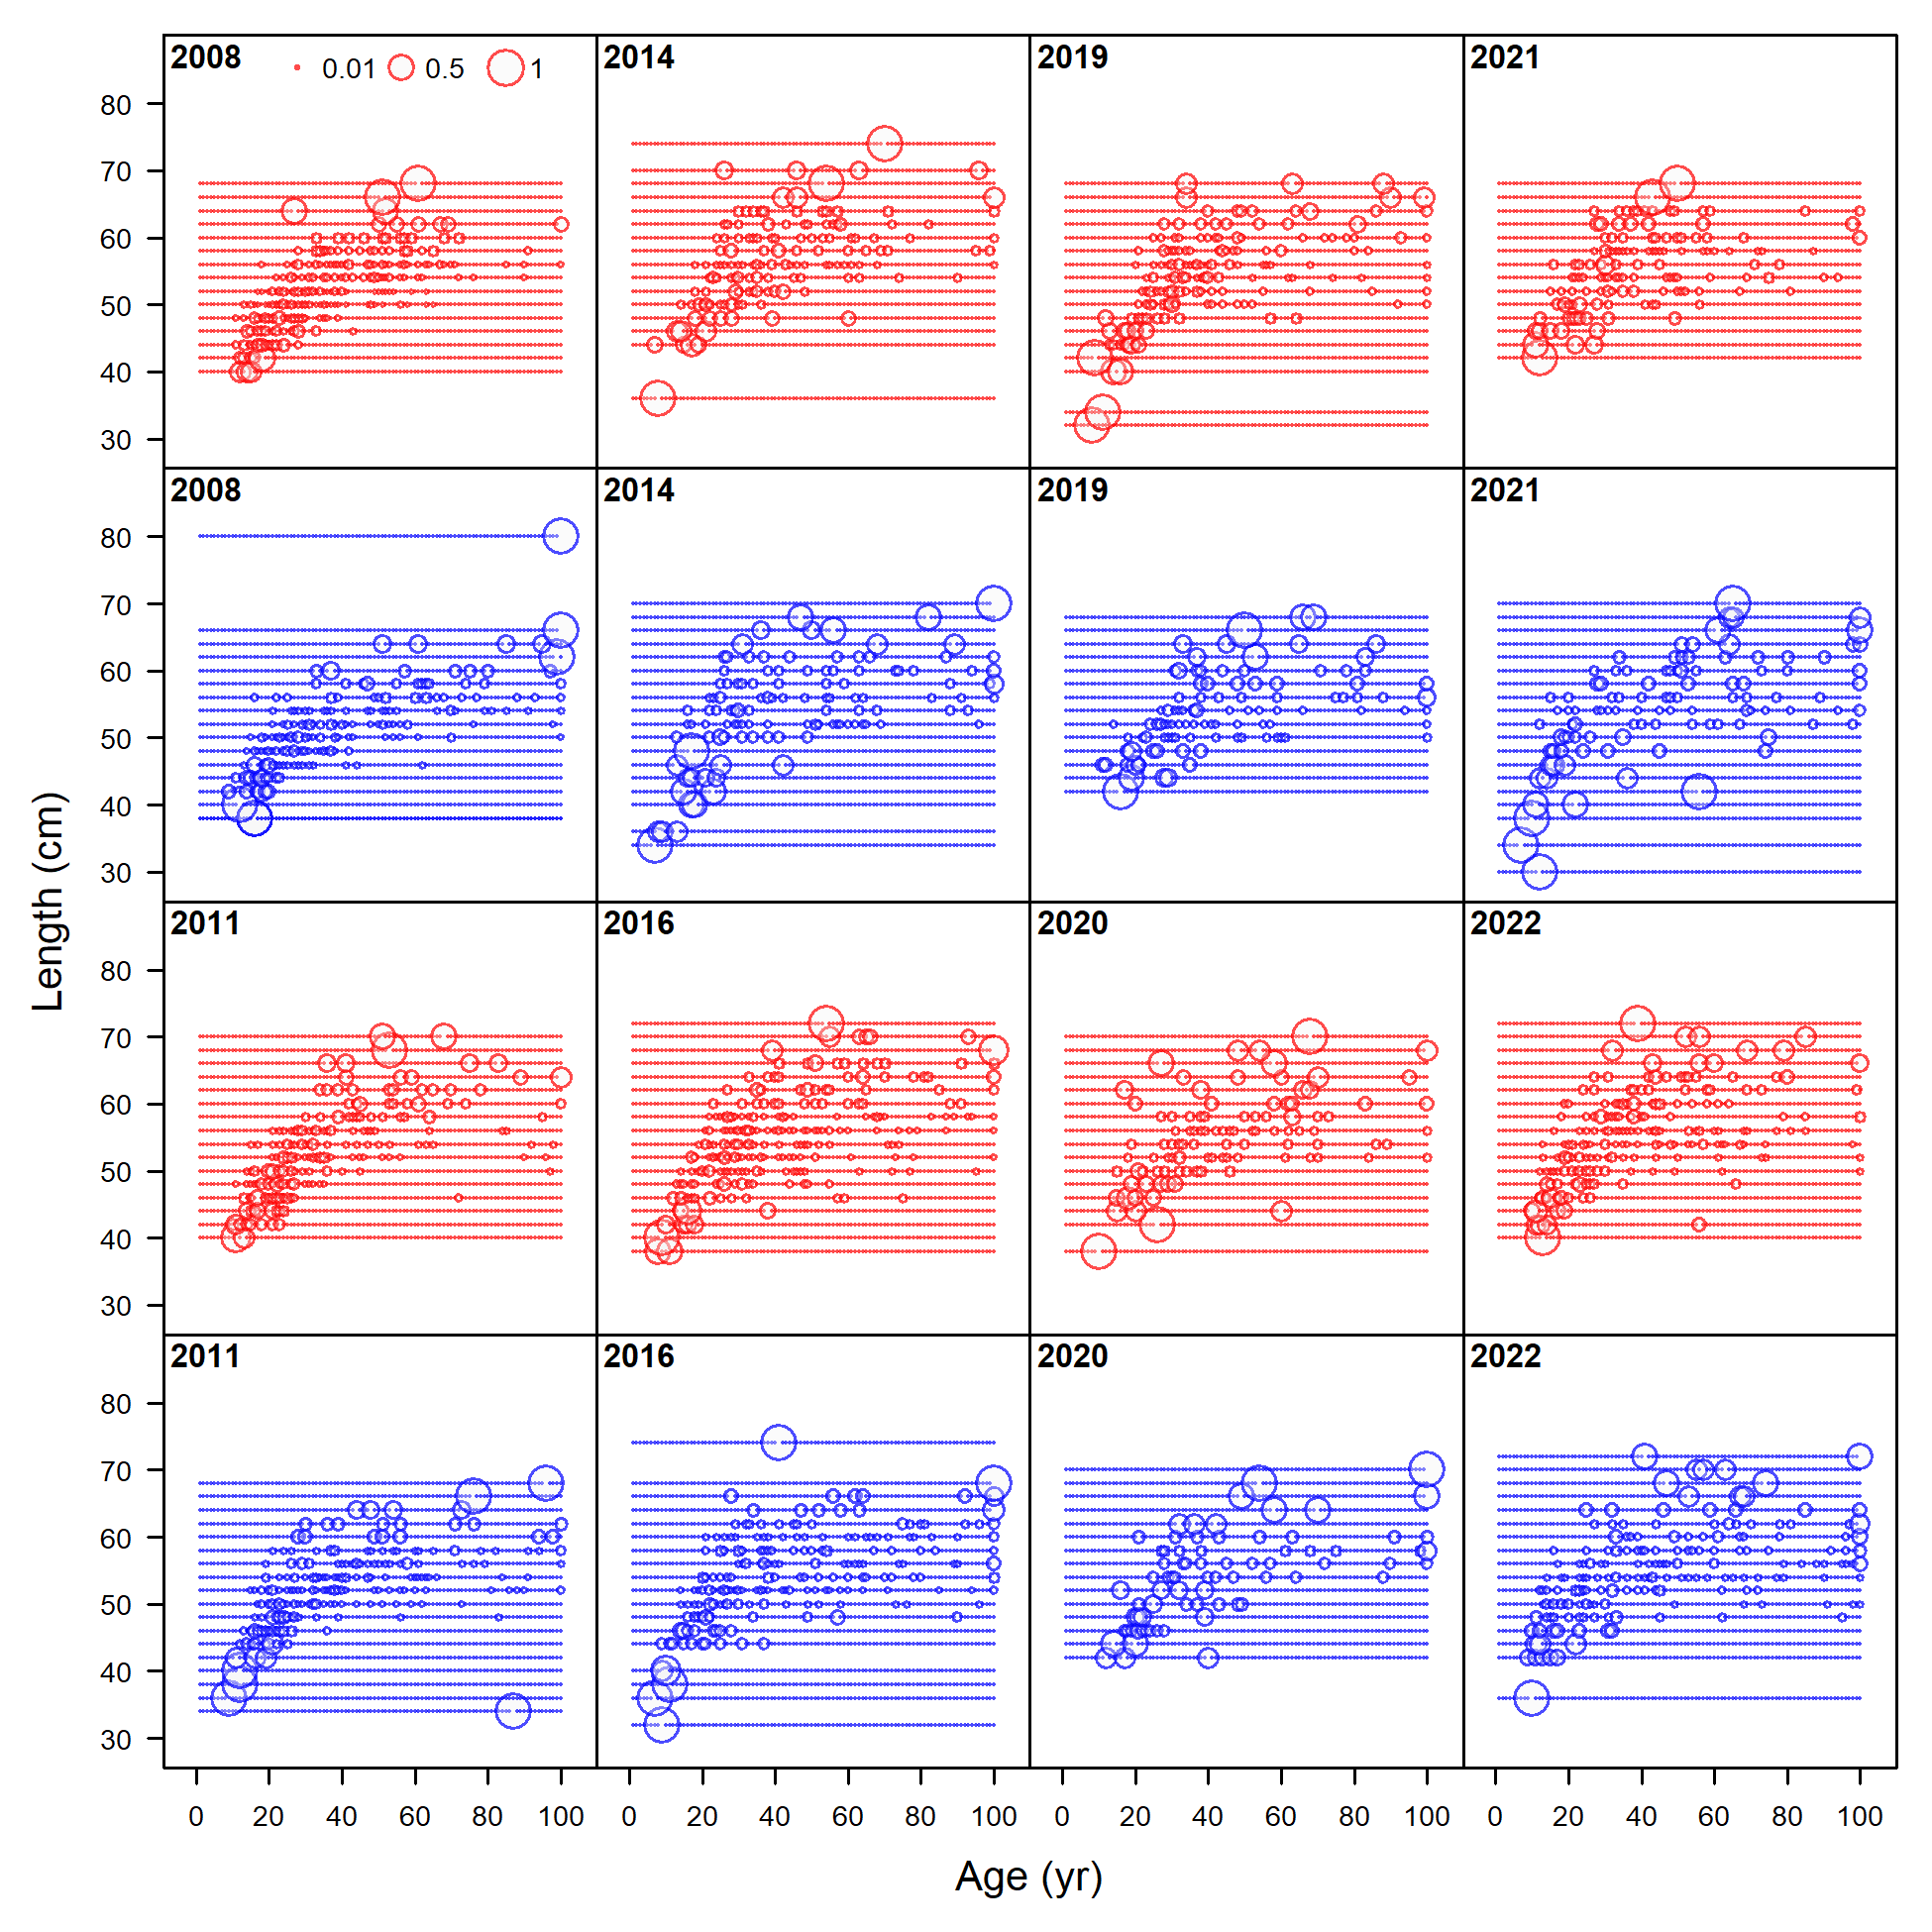
\includegraphics[keepaspectratio]{ref_model/plots/comp_condAALdat_bubflt6mkt0_page1.png}}

}

\caption{\label{fig-caal_flt6_1}Conditional ages-at-length composition
data for At-Sea Hake fleet.}

\end{figure}%

\begin{figure}[H]

\centering{

\pandocbounded{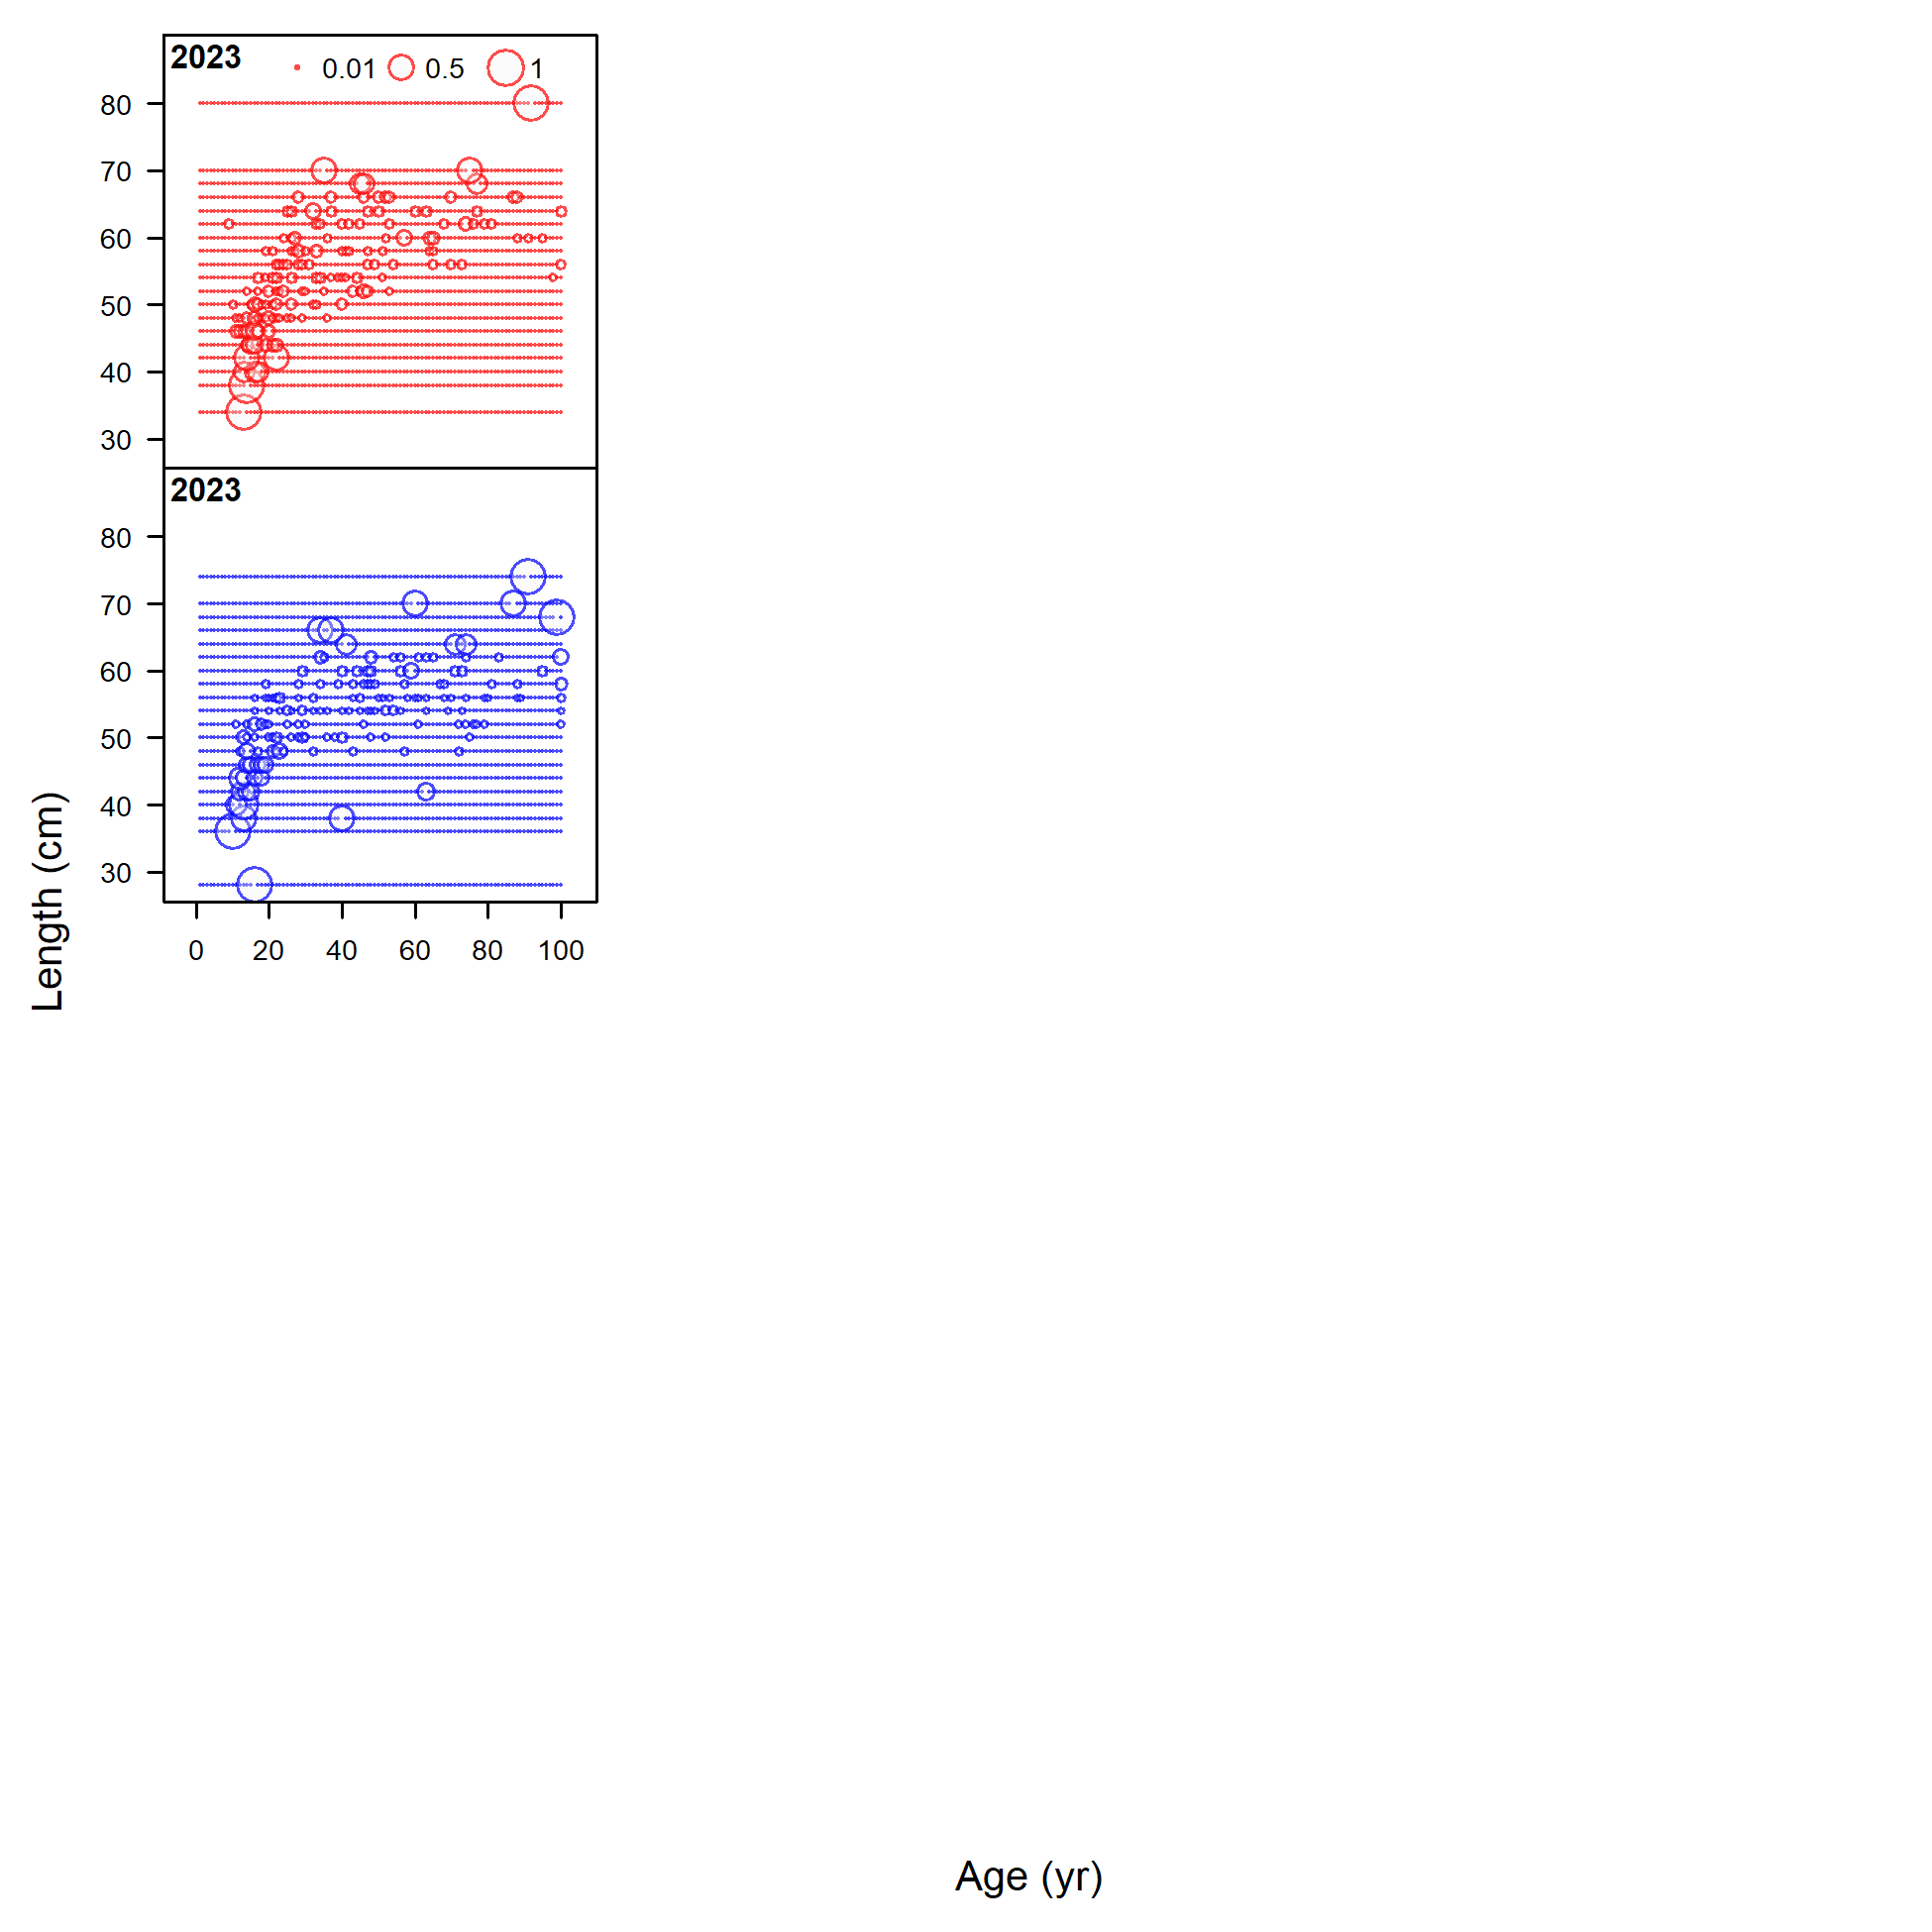
\includegraphics[keepaspectratio]{ref_model/plots/comp_condAALdat_bubflt6mkt0_page2.png}}

}

\caption{\label{fig-caal_flt6_2}Conditional ages-at-length composition
data for At-Sea Hake fleet, continued.}

\end{figure}%

\begin{figure}[H]

\centering{

\pandocbounded{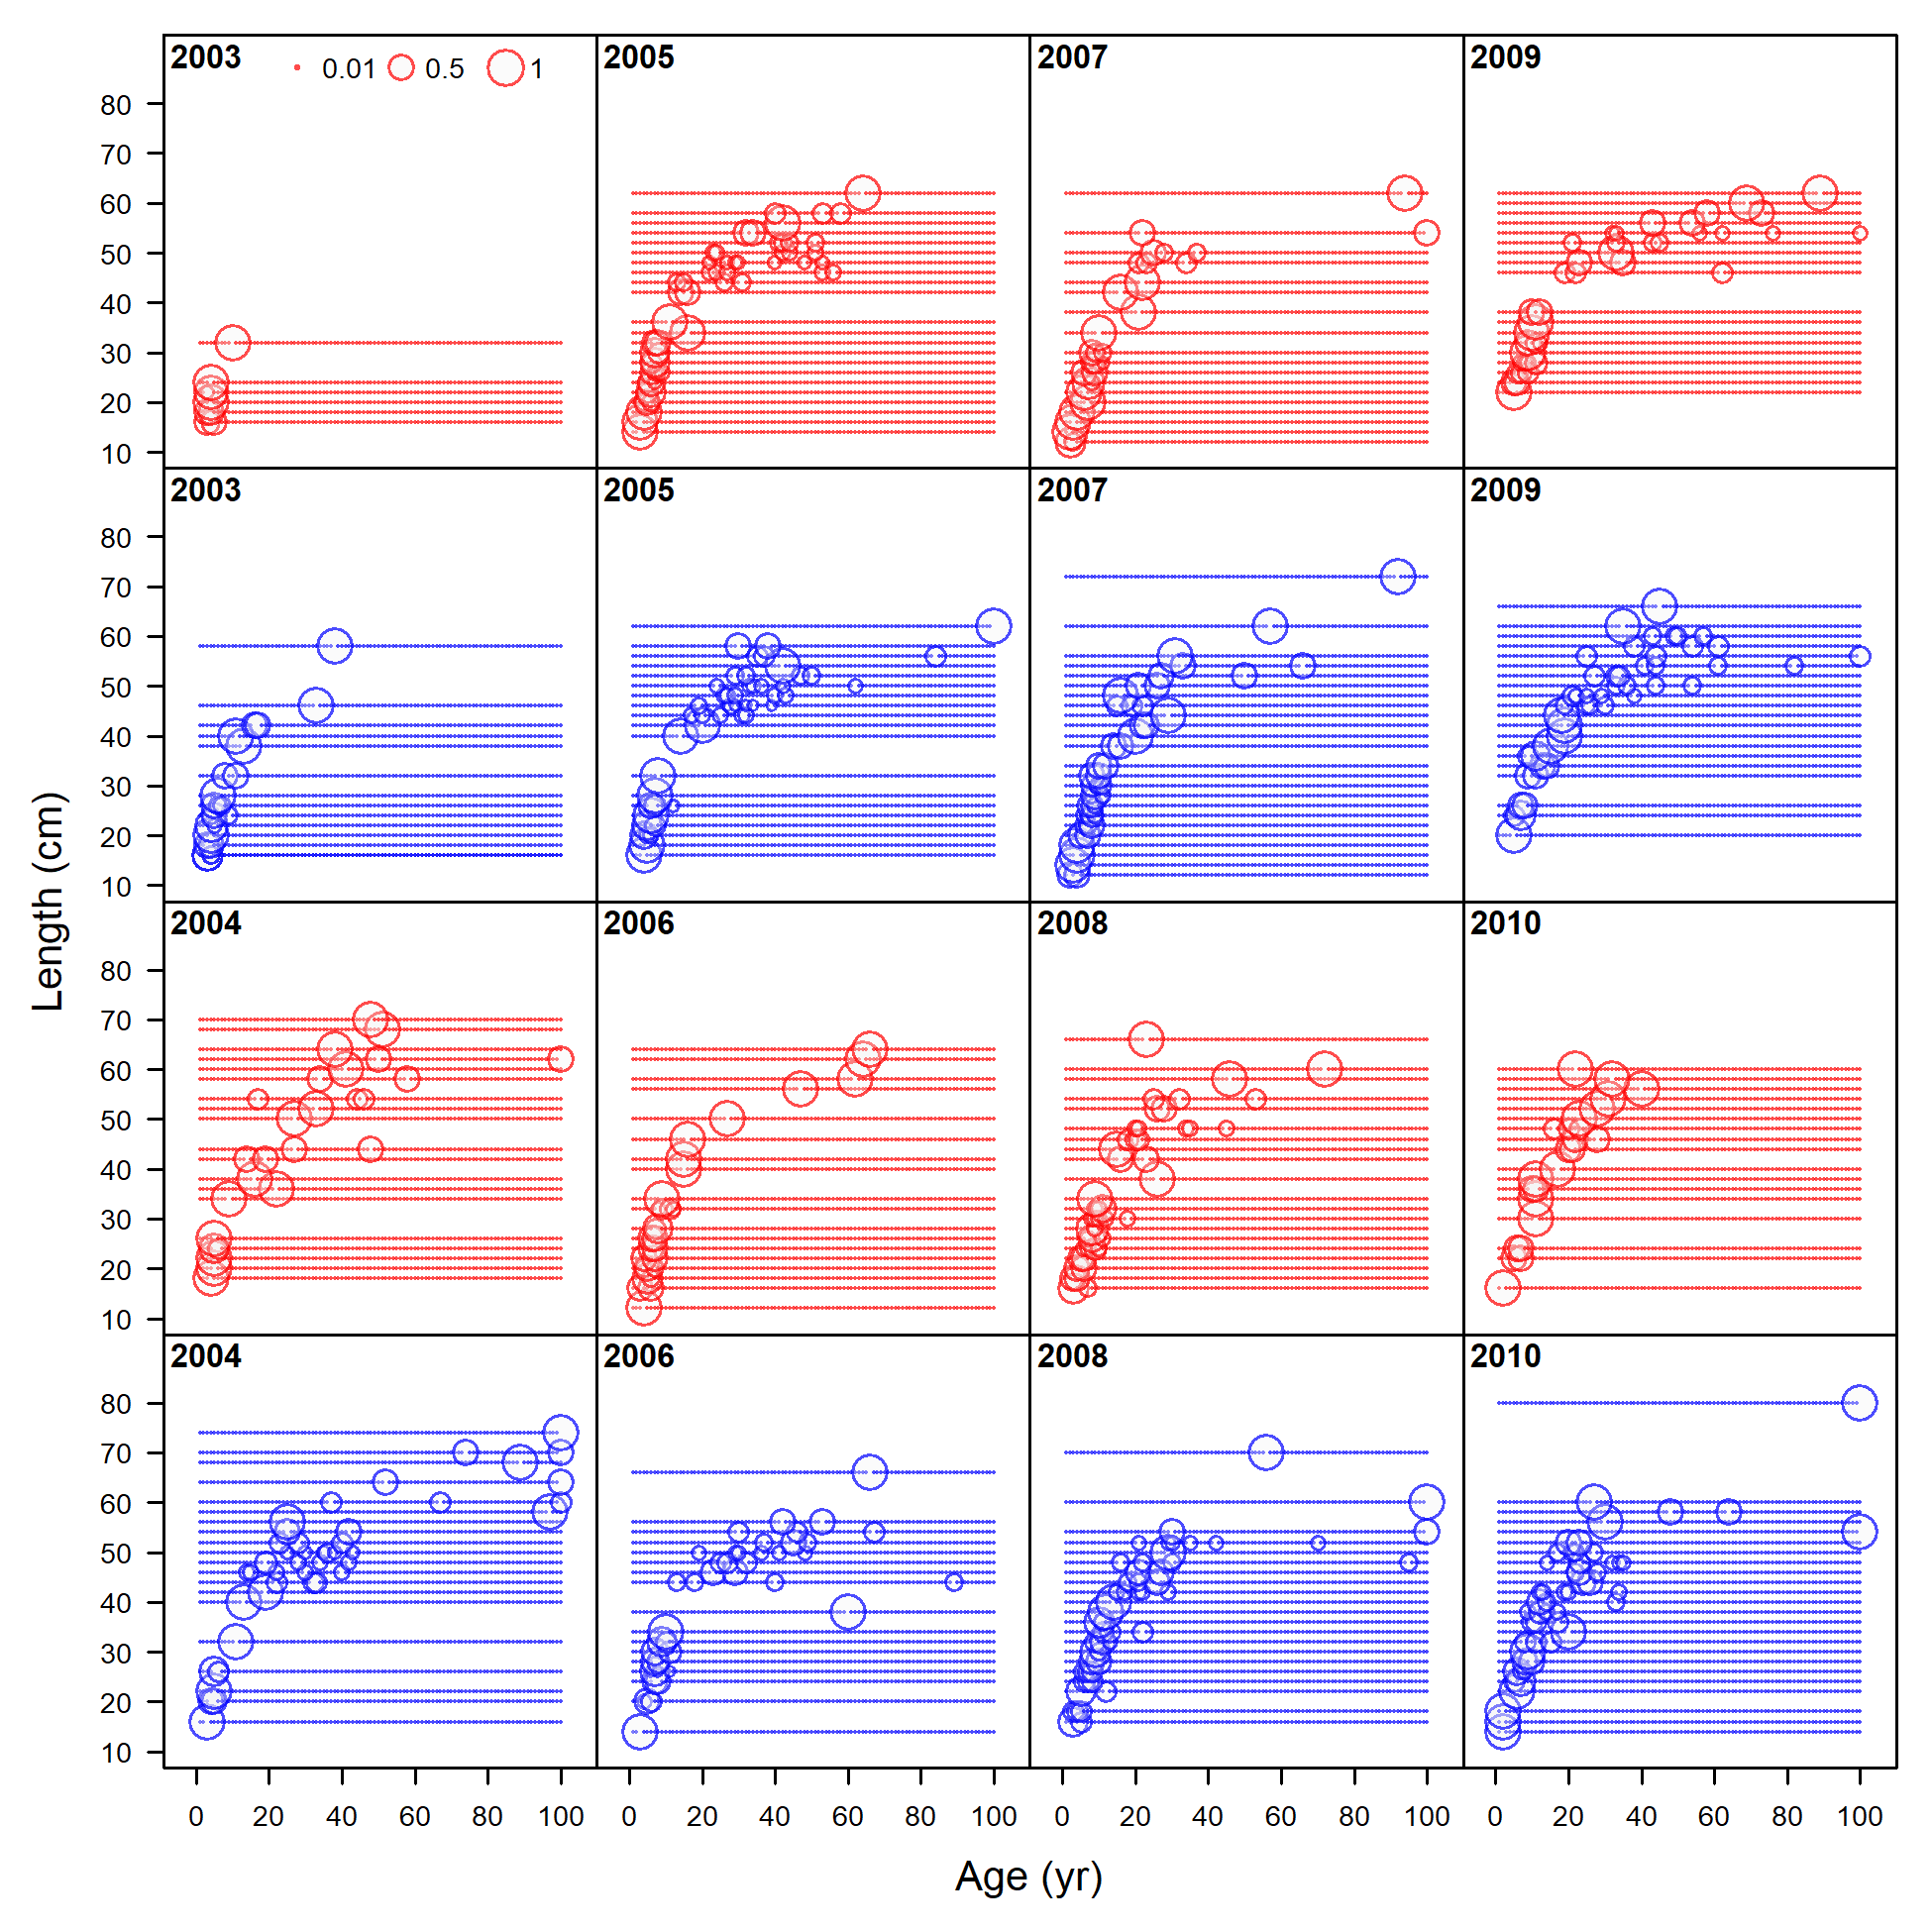
\includegraphics[keepaspectratio]{ref_model/plots/comp_condAALdat_bubflt10mkt0_page1.png}}

}

\caption{\label{fig-caal_flt10_1}Conditional ages-at-length composition
data for WCGBTS.}

\end{figure}%

\begin{figure}[H]

\centering{

\pandocbounded{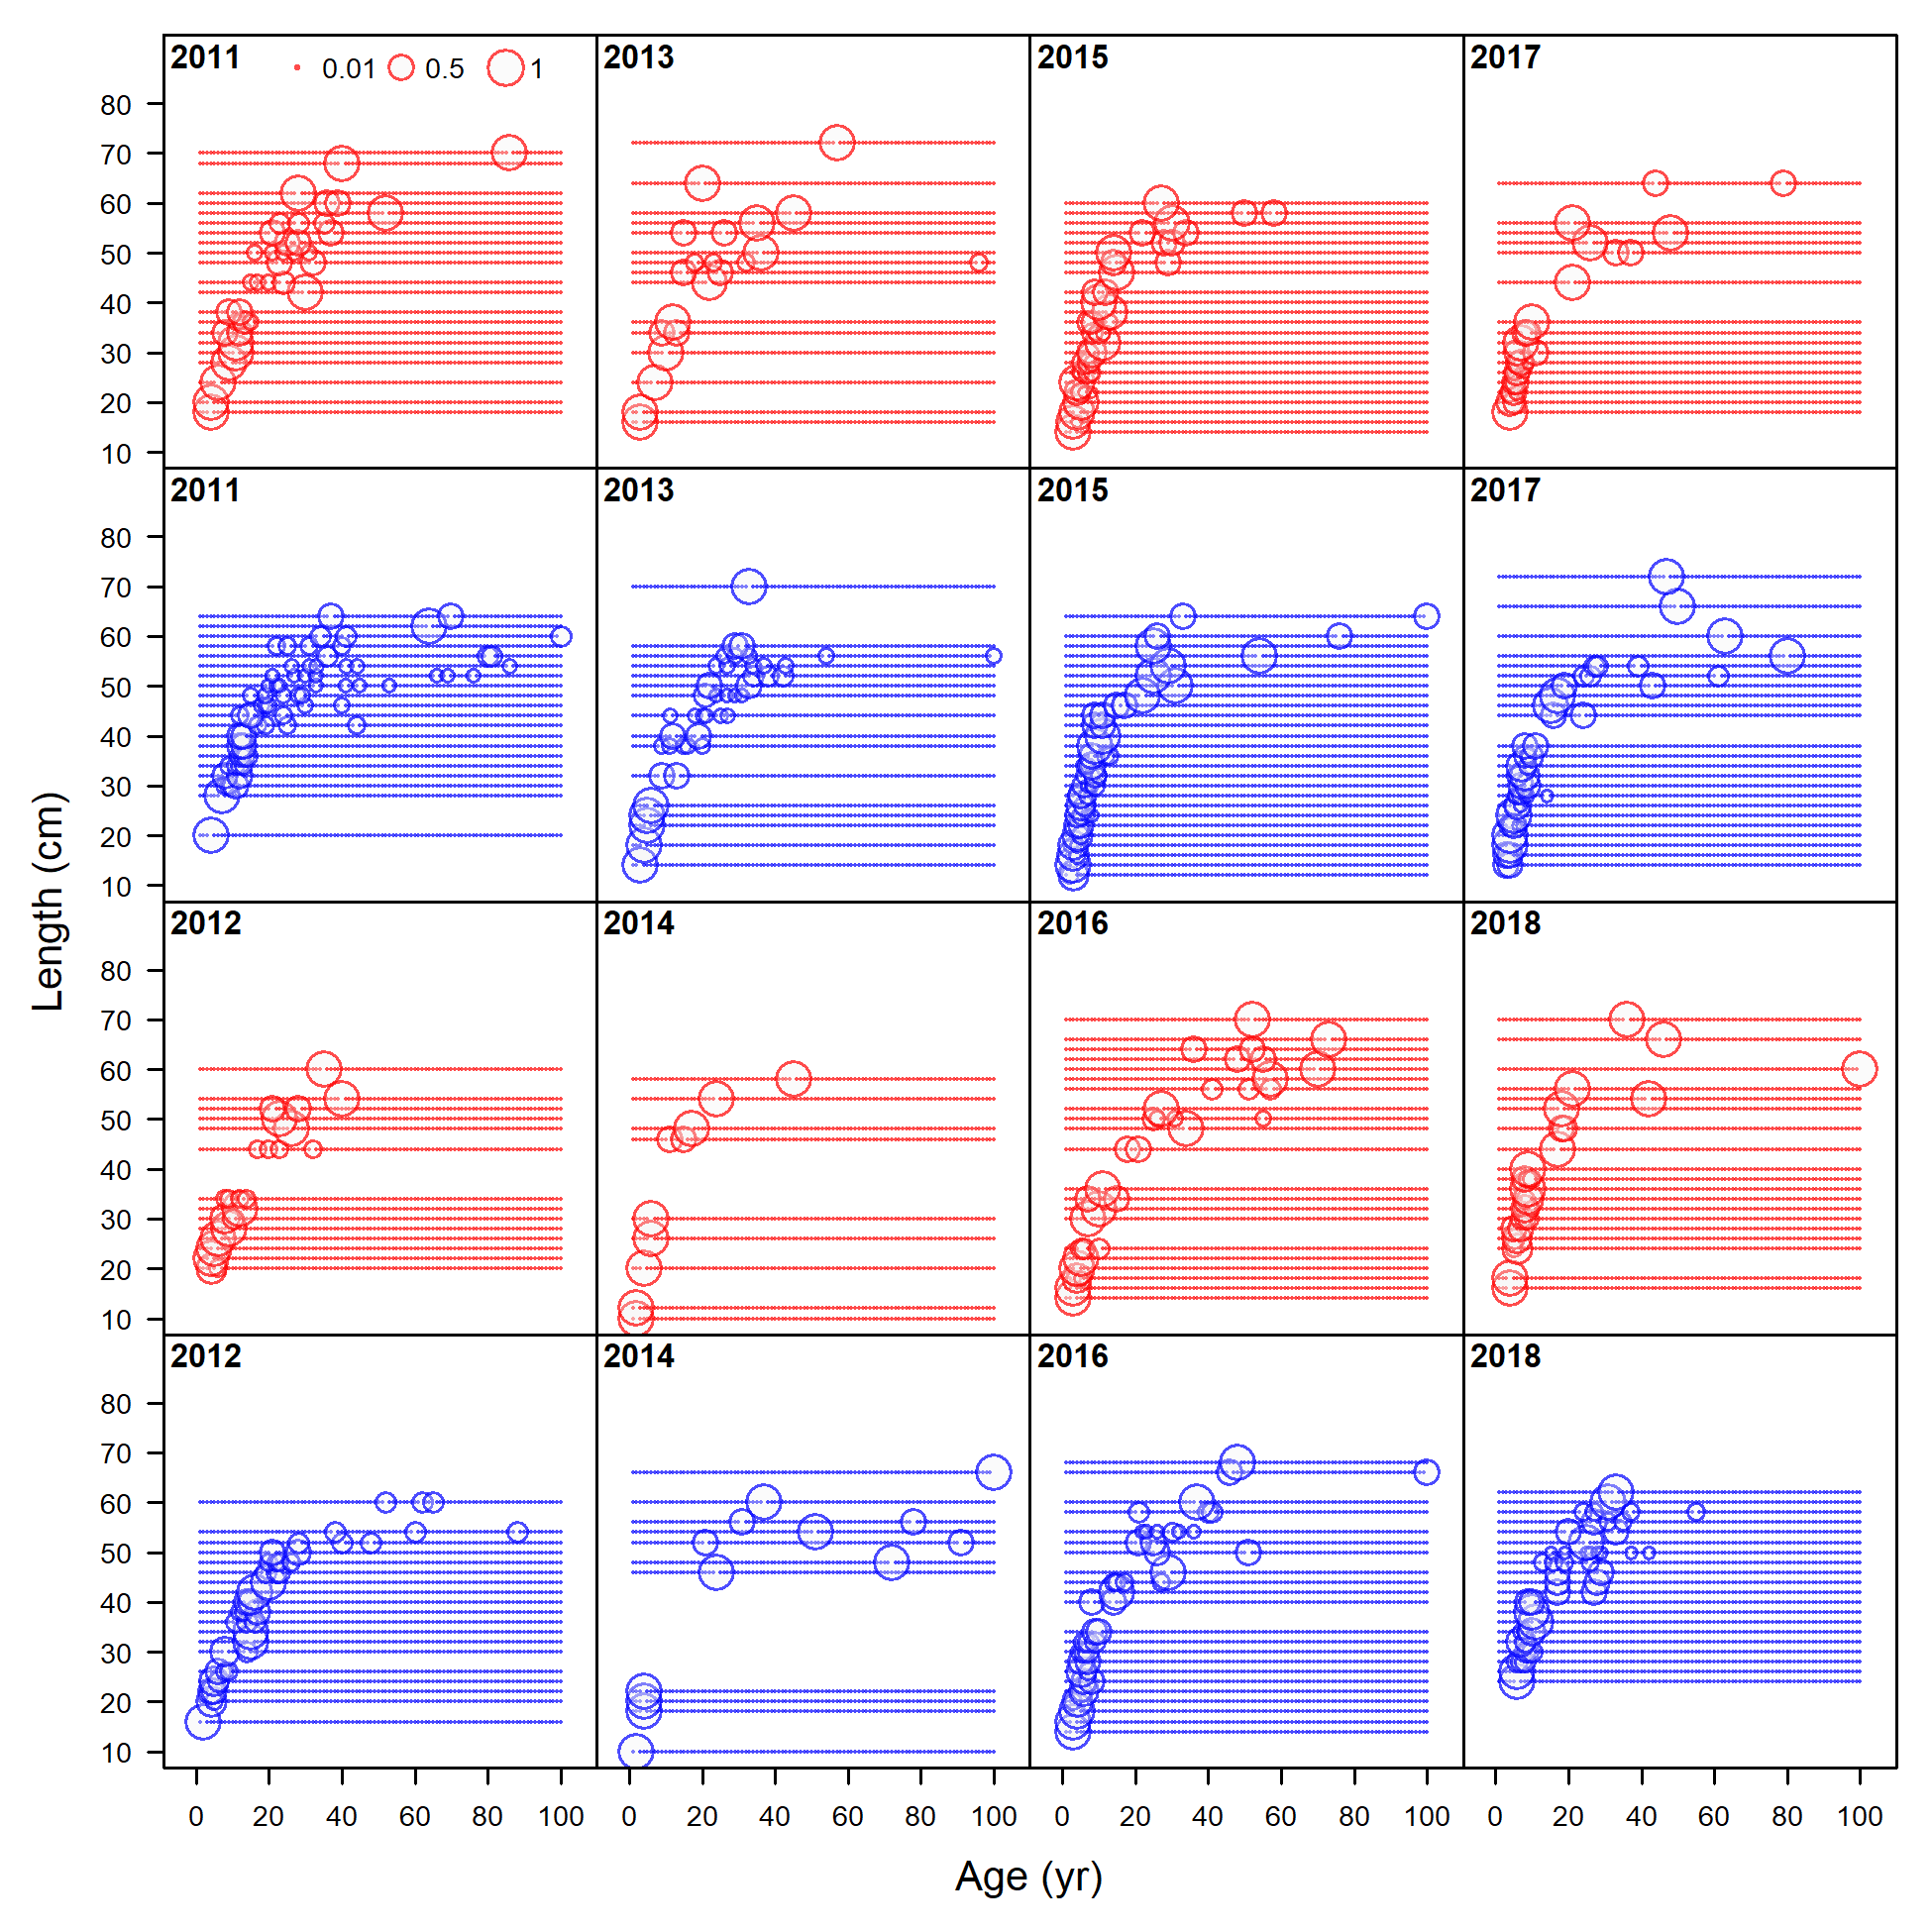
\includegraphics[keepaspectratio]{ref_model/plots/comp_condAALdat_bubflt10mkt0_page2.png}}

}

\caption{\label{fig-caal_flt10_2}Conditional ages-at-length composition
data for WCGBTS, continued.}

\end{figure}%

\begin{figure}[H]

\centering{

\pandocbounded{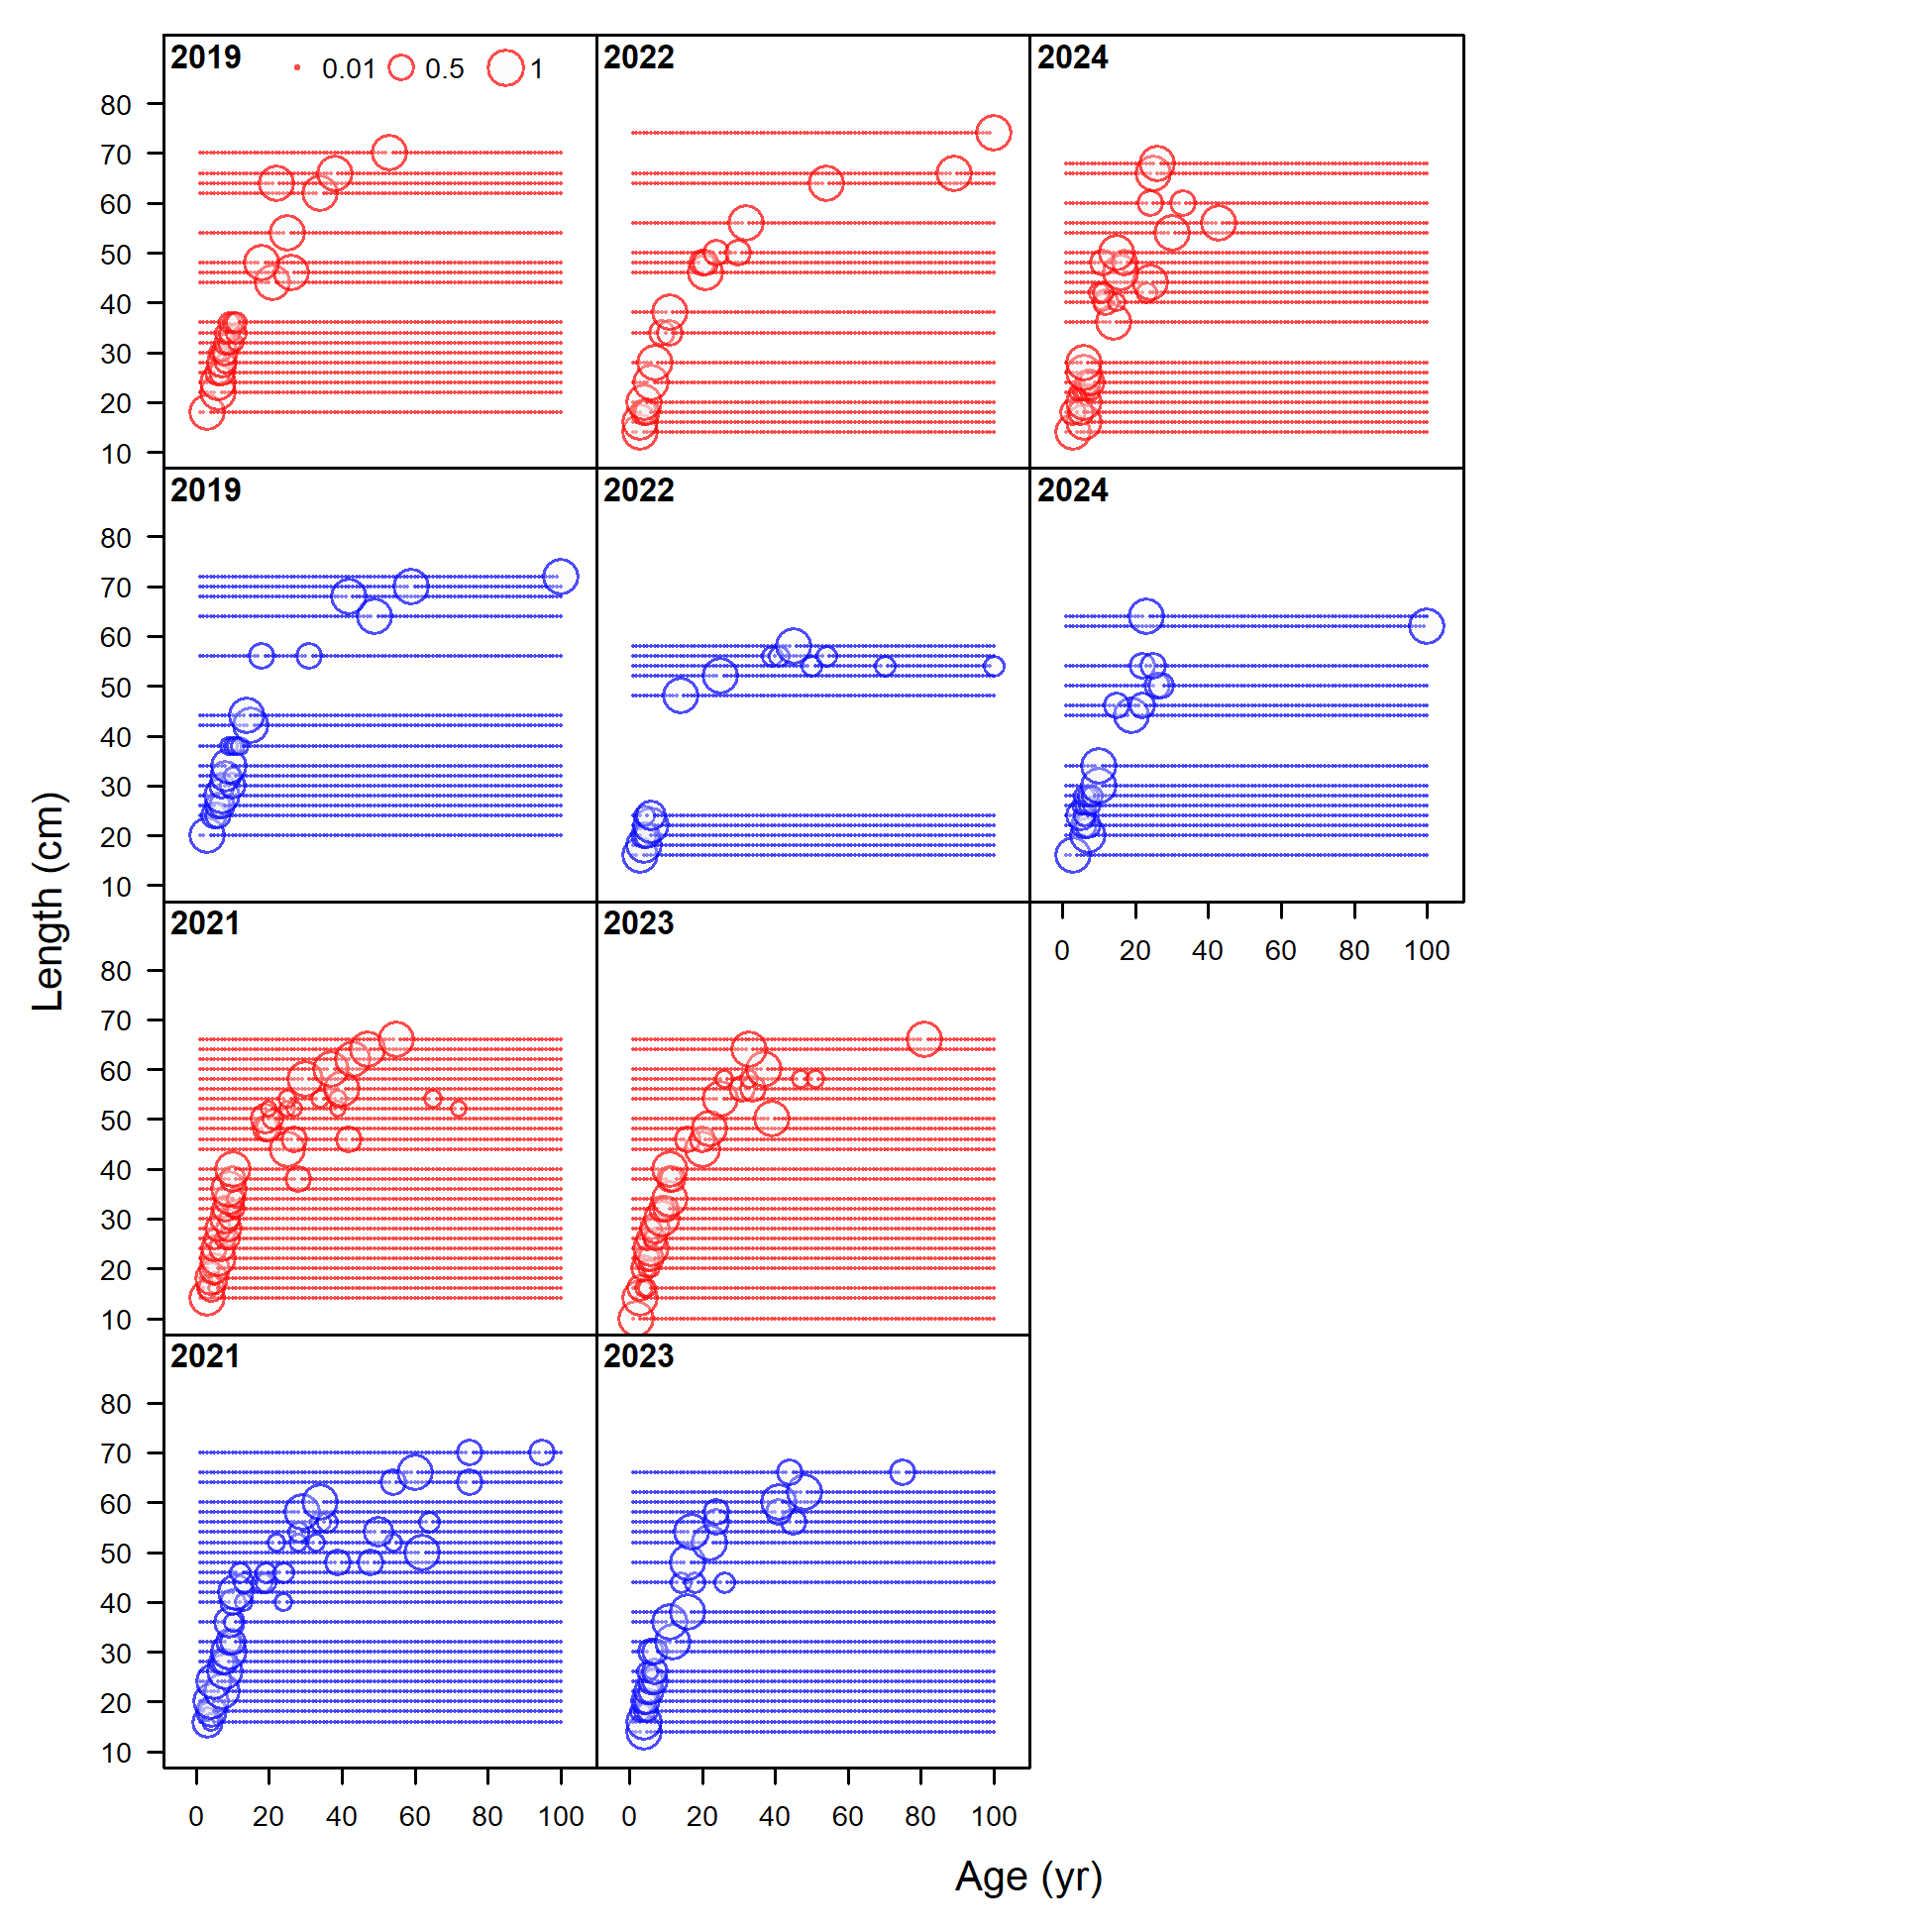
\includegraphics[keepaspectratio]{ref_model/plots/comp_condAALdat_bubflt10mkt0_page3.png}}

}

\caption{\label{fig-caal_flt10_3}Conditional ages-at-length composition
data for WCGBTS, continued.}

\end{figure}%

\begin{figure}[H]

\centering{

\pandocbounded{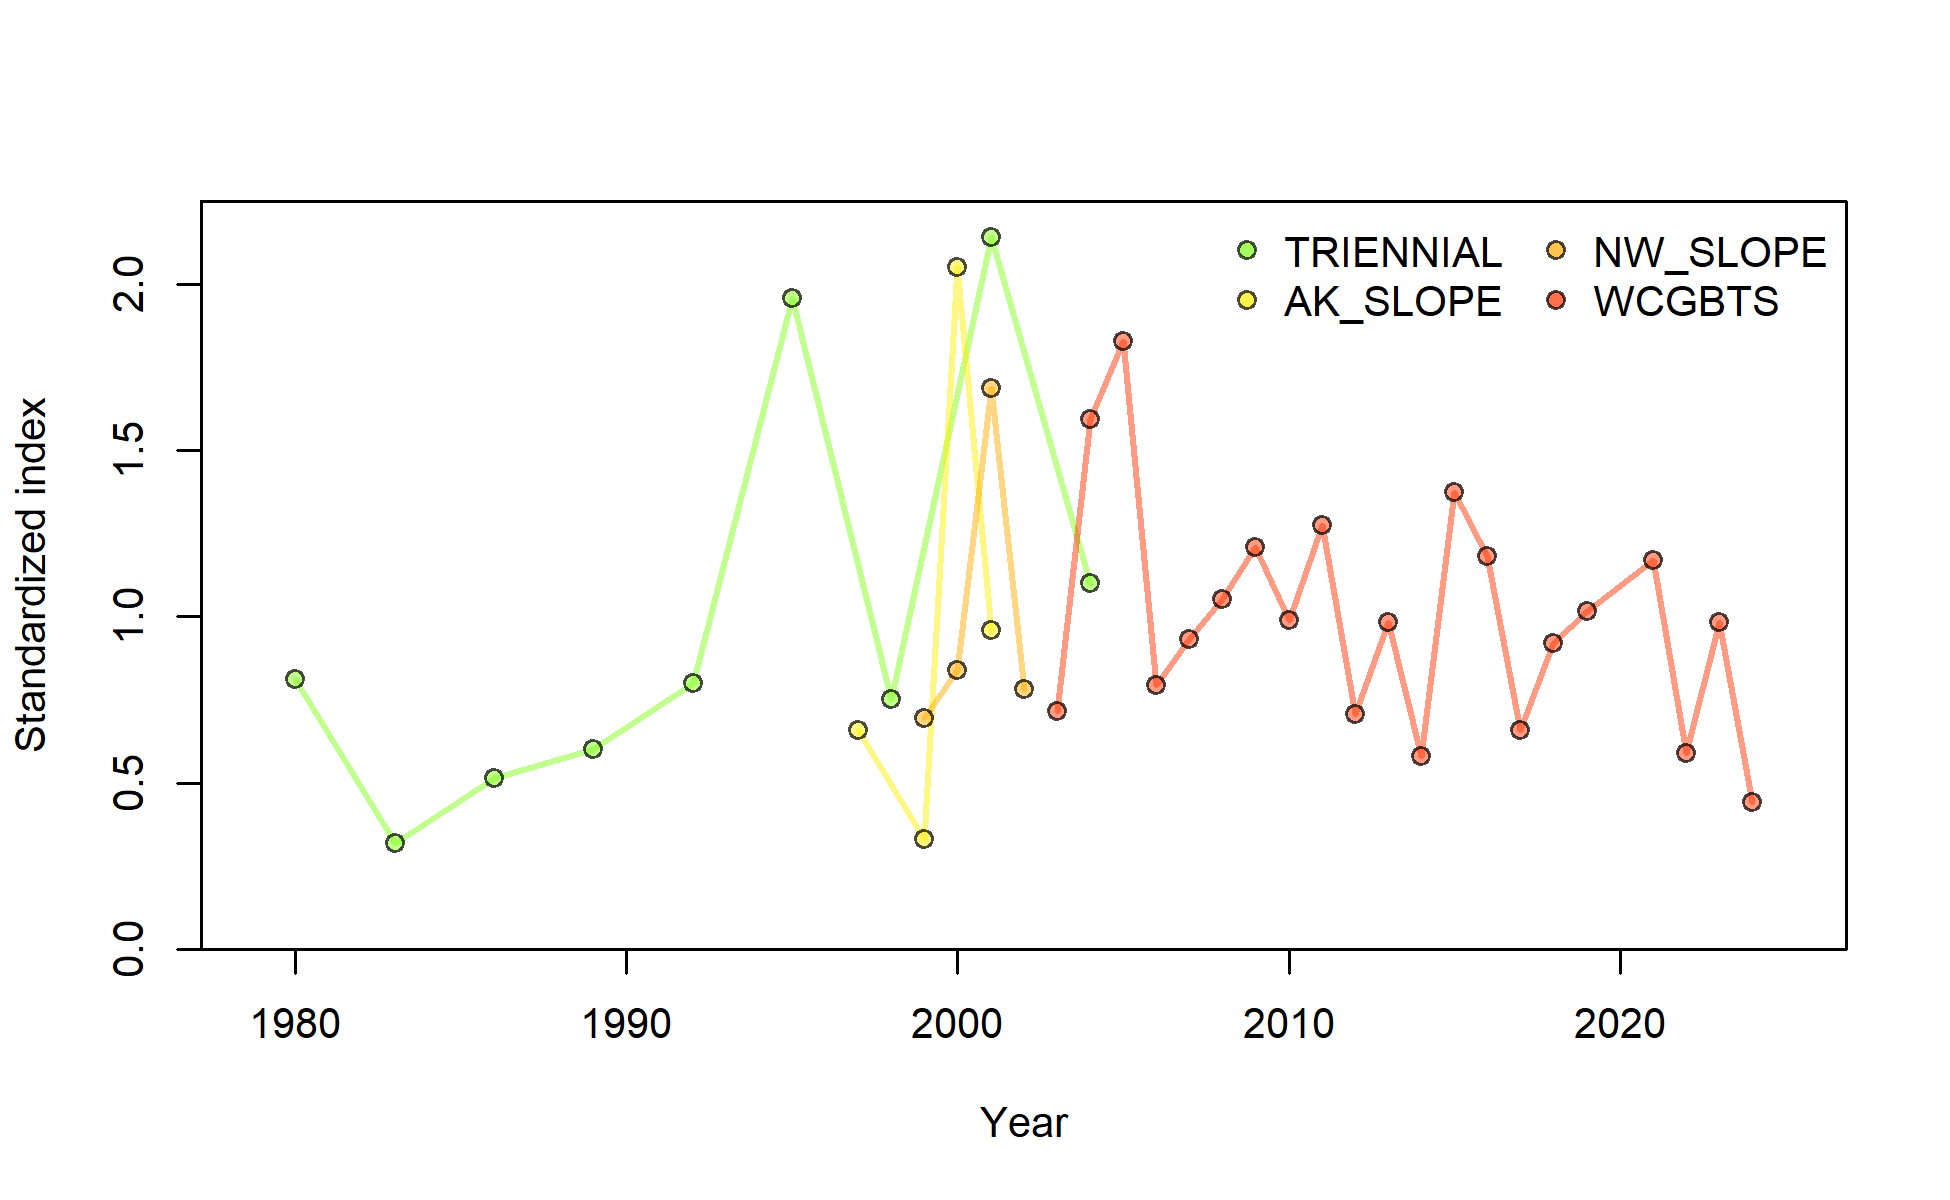
\includegraphics[keepaspectratio]{ref_model/plots/index9_standcpueall.png}}

}

\caption{\label{fig-All_indices}Standardized indices.}

\end{figure}%

\begin{figure}[H]

\centering{

\pandocbounded{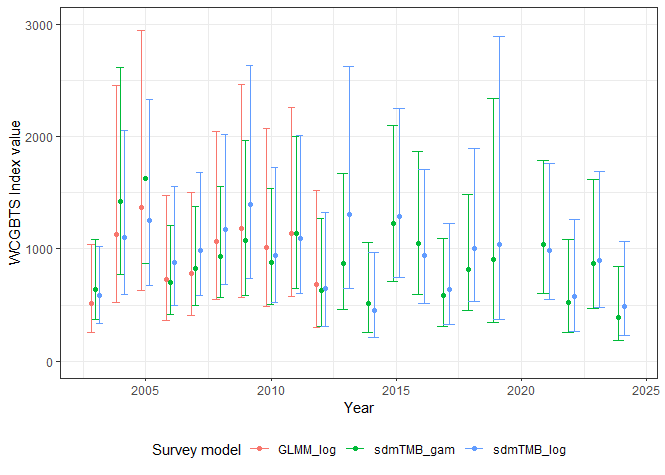
\includegraphics[keepaspectratio]{plots_4_doc/WCGBTS_comps.png}}

}

\caption{\label{fig-WCGBTS_comparison}Comparison of the West Coast
Groundfish Bottom Trawl Survey (WCGBTS) index from the previous
assessment (GLMM) and the WCGBTS index of abundance used in this
assessment (sdmTMB, lognormal distribution).}

\end{figure}%

\begin{figure}[H]

\centering{

\pandocbounded{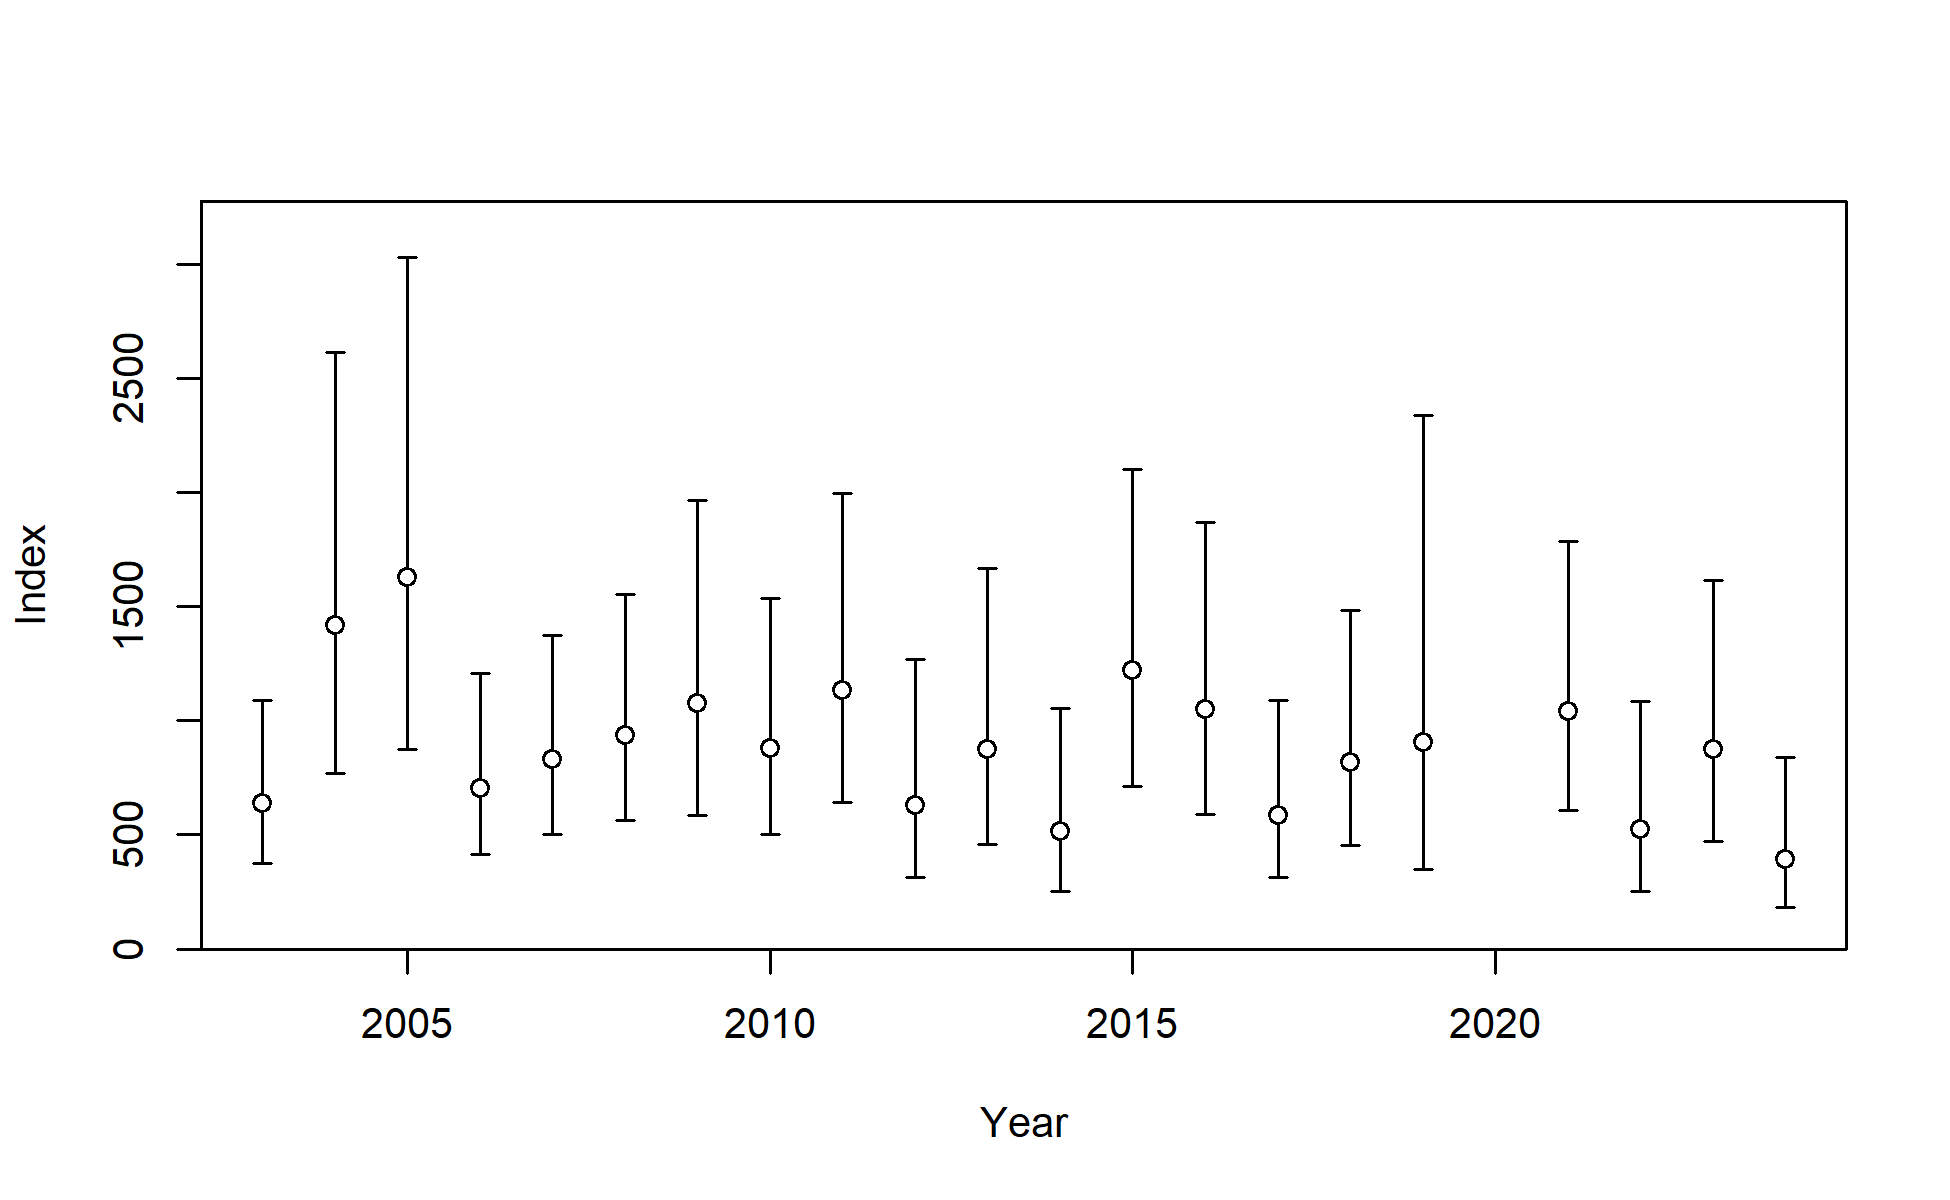
\includegraphics[keepaspectratio]{ref_model/plots/index1_cpuedata_WCGBTS.png}}

}

\caption{\label{fig-WCGBTS_index}WCGBTS index.}

\end{figure}%

\begin{figure}[H]

\centering{

\pandocbounded{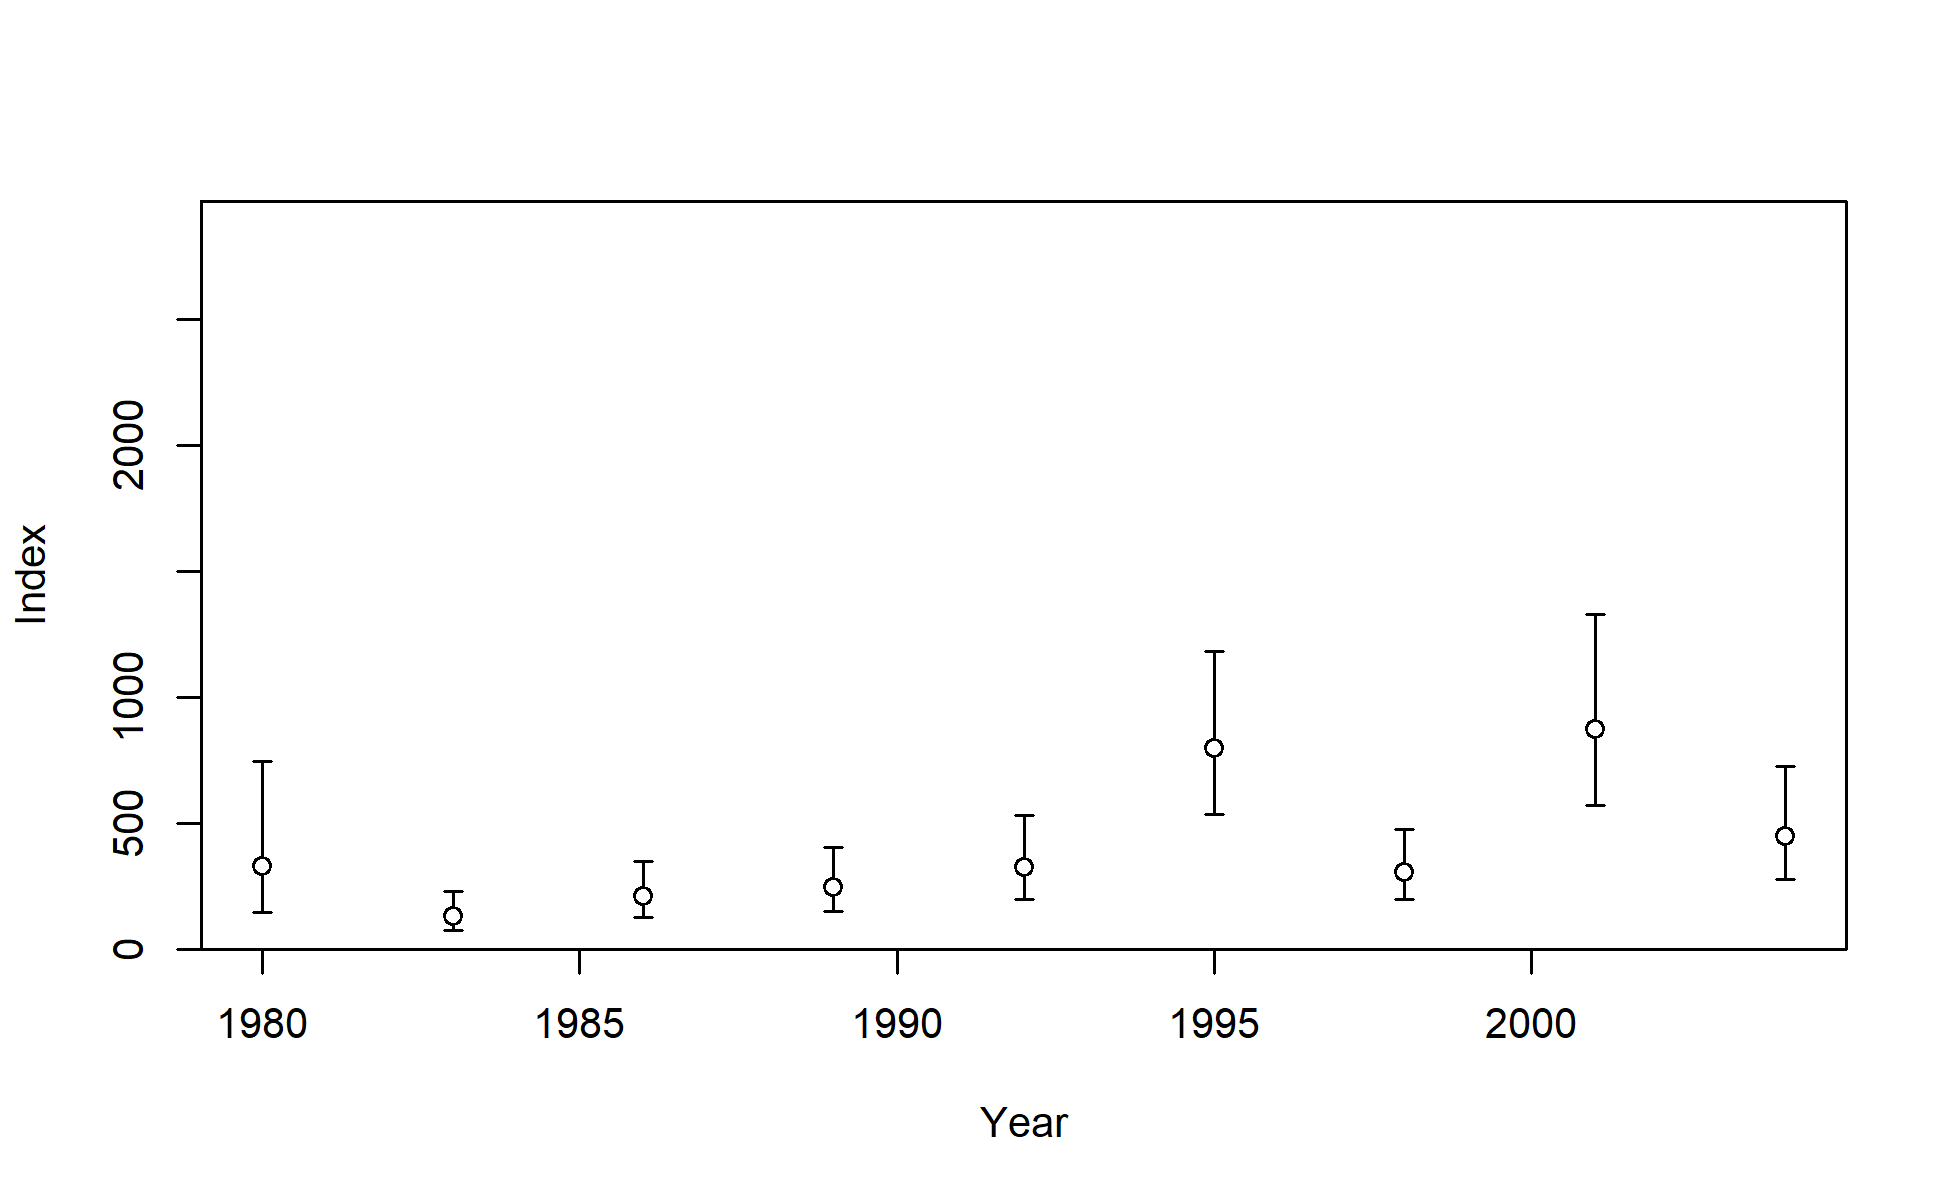
\includegraphics[keepaspectratio]{ref_model/plots/index1_cpuedata_TRIENNIAL.png}}

}

\caption{\label{fig-Triennial_index}Triennial Survey index.}

\end{figure}%

\begin{figure}[H]

\centering{

\pandocbounded{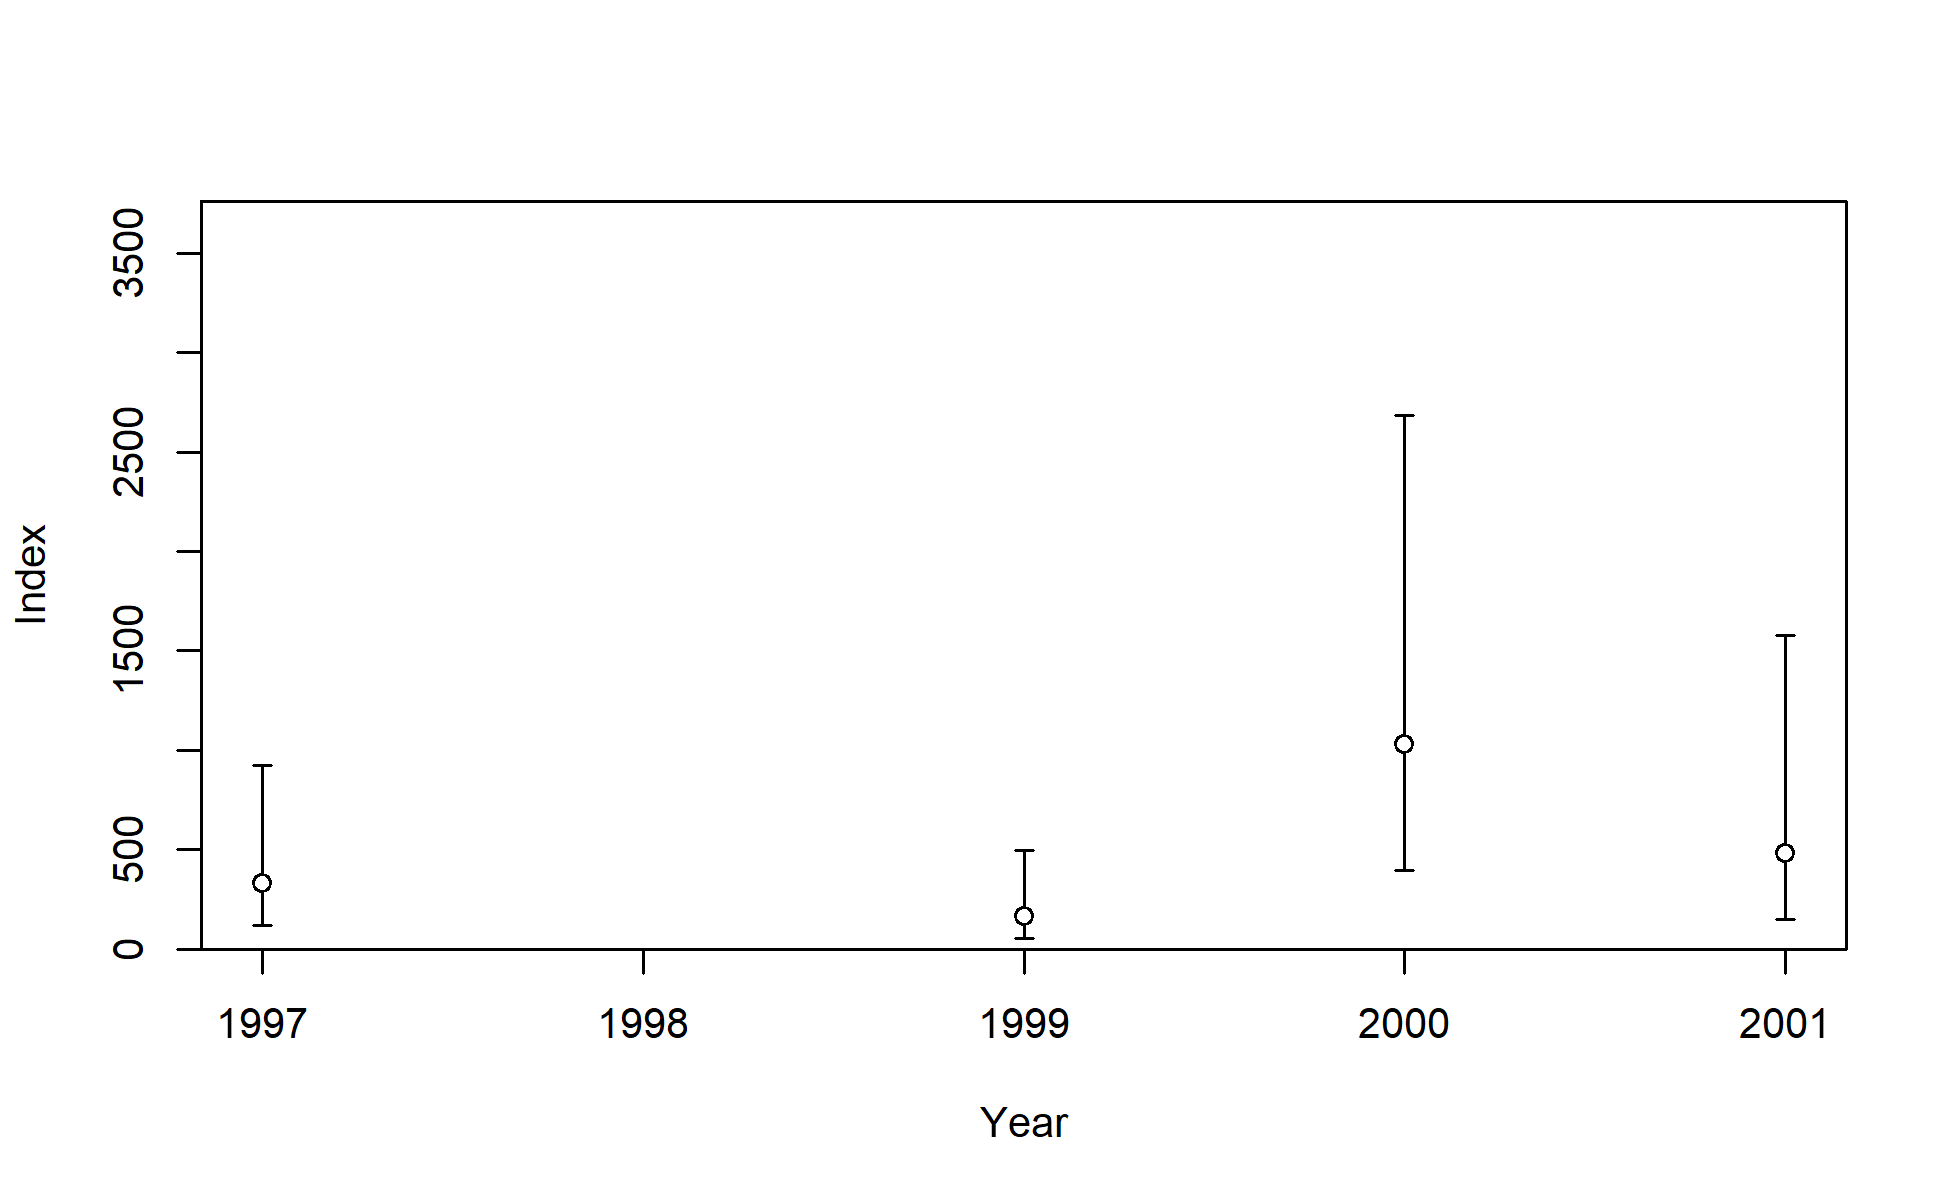
\includegraphics[keepaspectratio]{ref_model/plots/index1_cpuedata_AK_SLOPE.png}}

}

\caption{\label{fig-AFSC_Slope_index}AFSC Slope Survey index.}

\end{figure}%

\begin{figure}[H]

\centering{

\pandocbounded{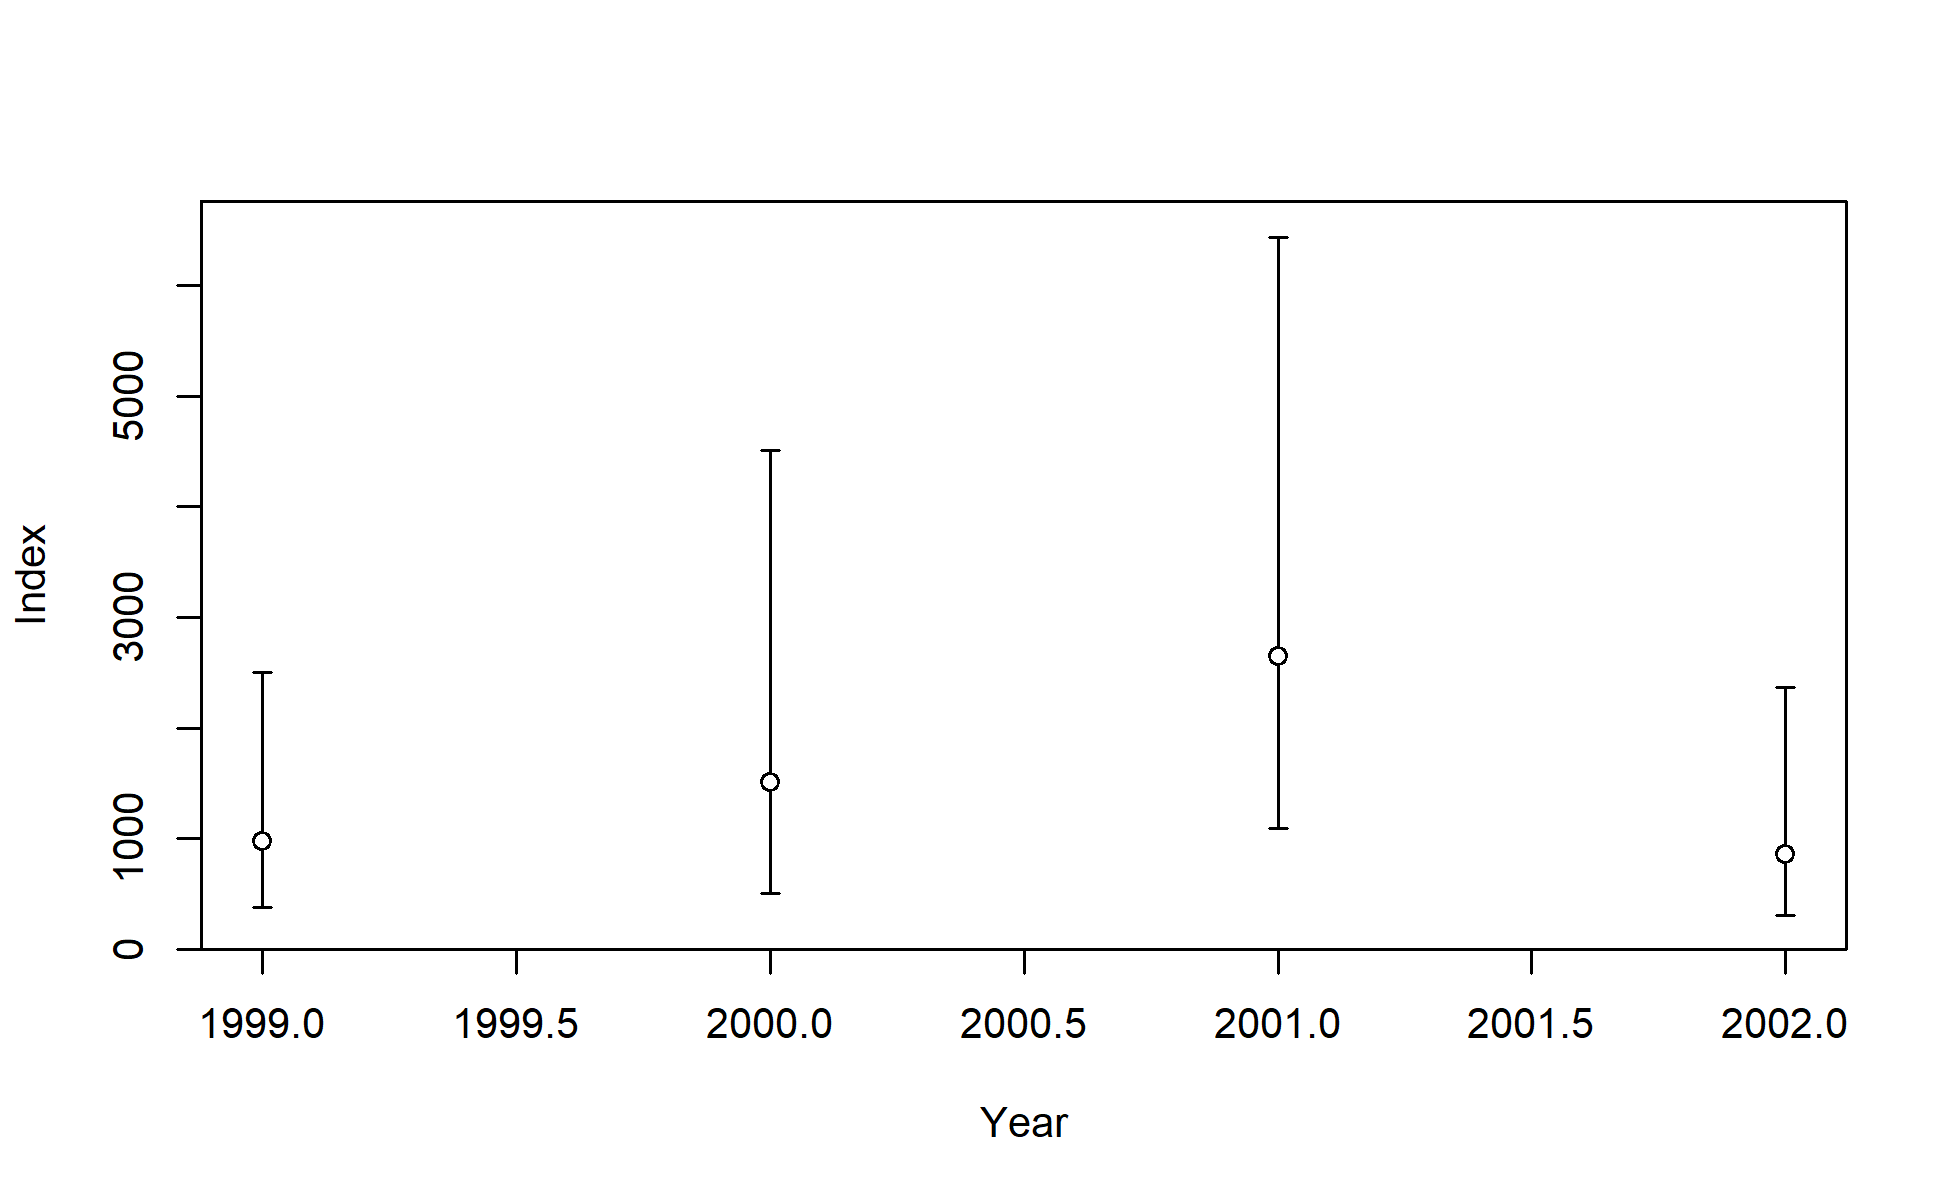
\includegraphics[keepaspectratio]{ref_model/plots/index1_cpuedata_NW_SLOPE.png}}

}

\caption{\label{fig-NWFSC_Slope_index}NWFSC Slope Survey index.}

\end{figure}%

\begin{figure}[H]

\centering{

\pandocbounded{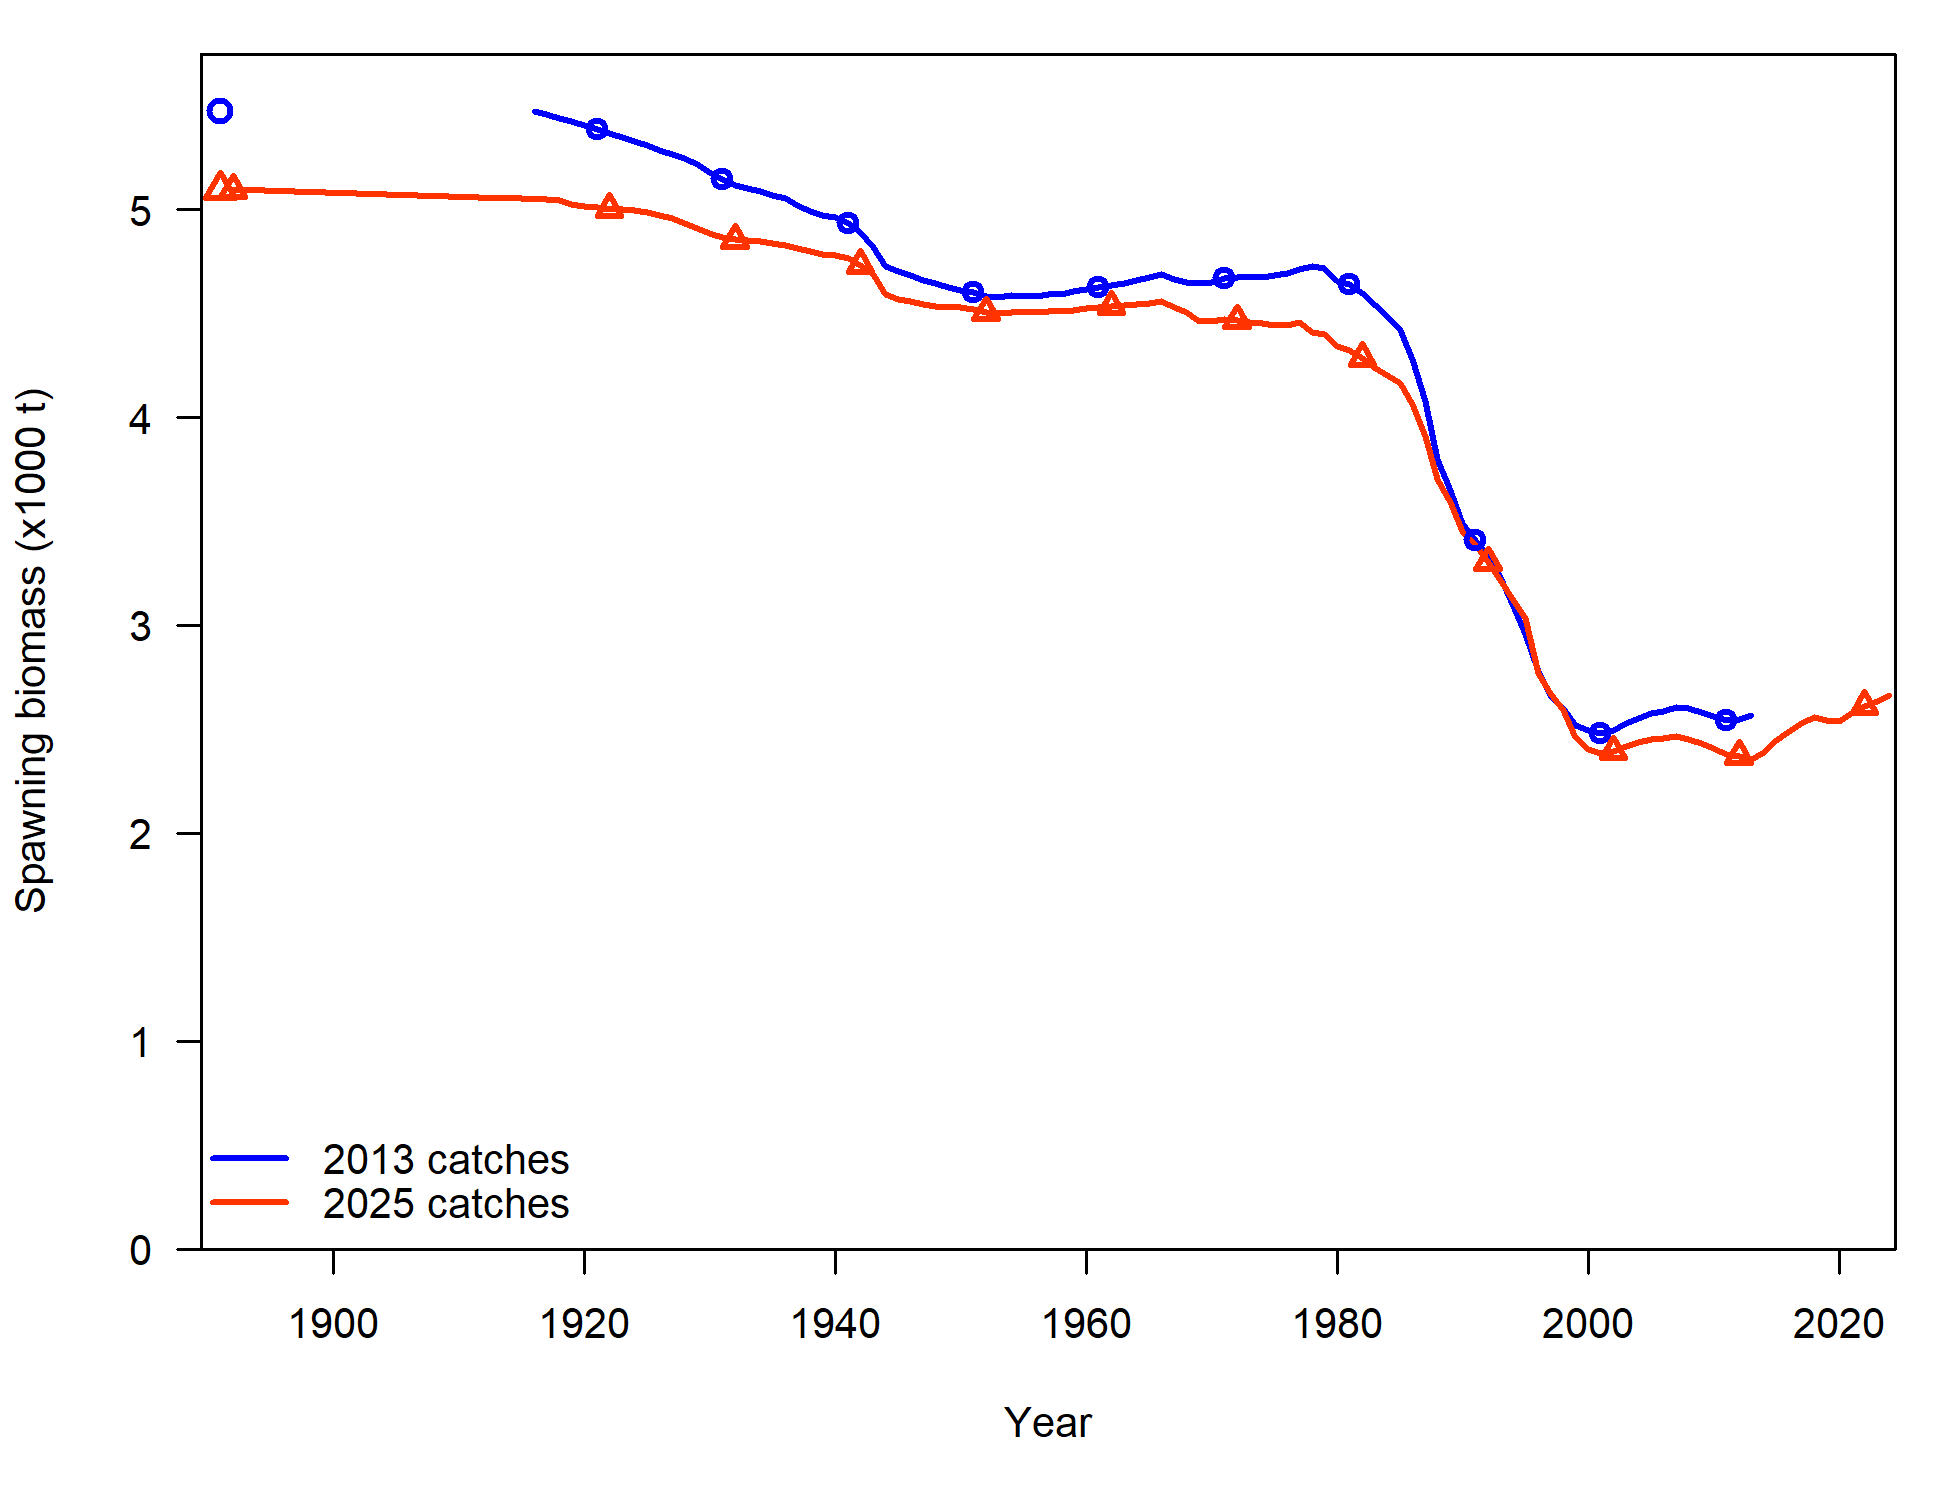
\includegraphics[keepaspectratio]{plots_4_doc/compare1_spawnbio_updatedCt.png}}

}

\caption{\label{fig-Ct_compsSO}Comparison of spawning output using
updated catches vs using catches from the 2013 Rougheye/Blackspotted
Rockfishes assessment.}

\end{figure}%

\begin{figure}[H]

\centering{

\pandocbounded{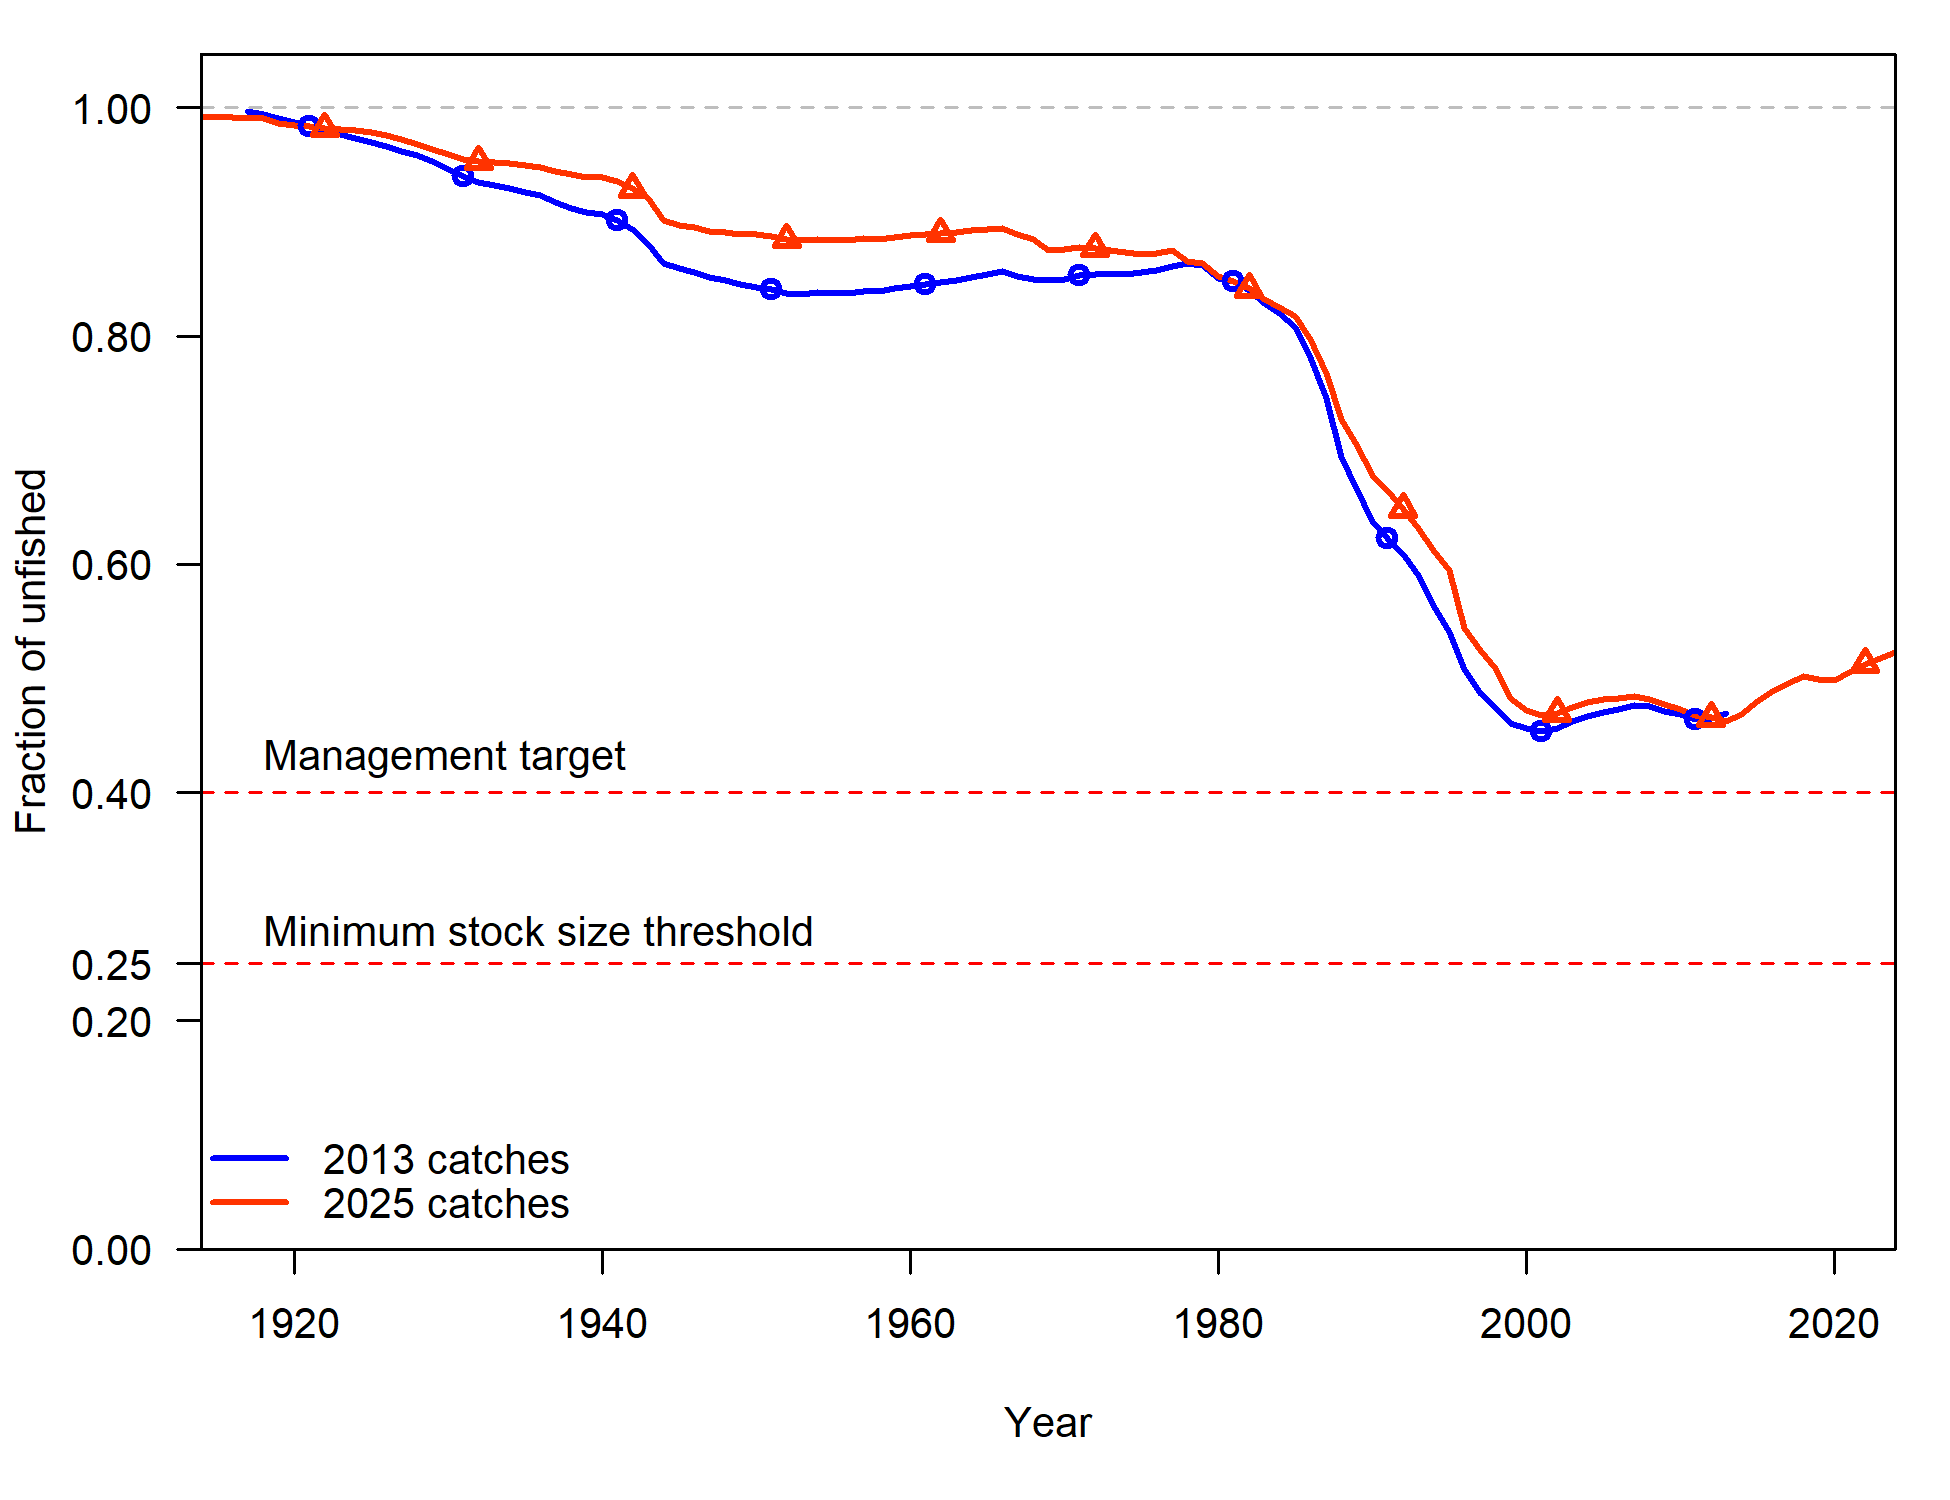
\includegraphics[keepaspectratio]{plots_4_doc/compare3_Bratio_updatedCt.png}}

}

\caption{\label{fig-Ct_compsRSS}Comparison of relative spawning output
using updated catches vs using catches from the 2013
Rougheye/Blackspotted Rockfishes assessment.}

\end{figure}%

\newpage

\begin{figure}[H]

\centering{

\pandocbounded{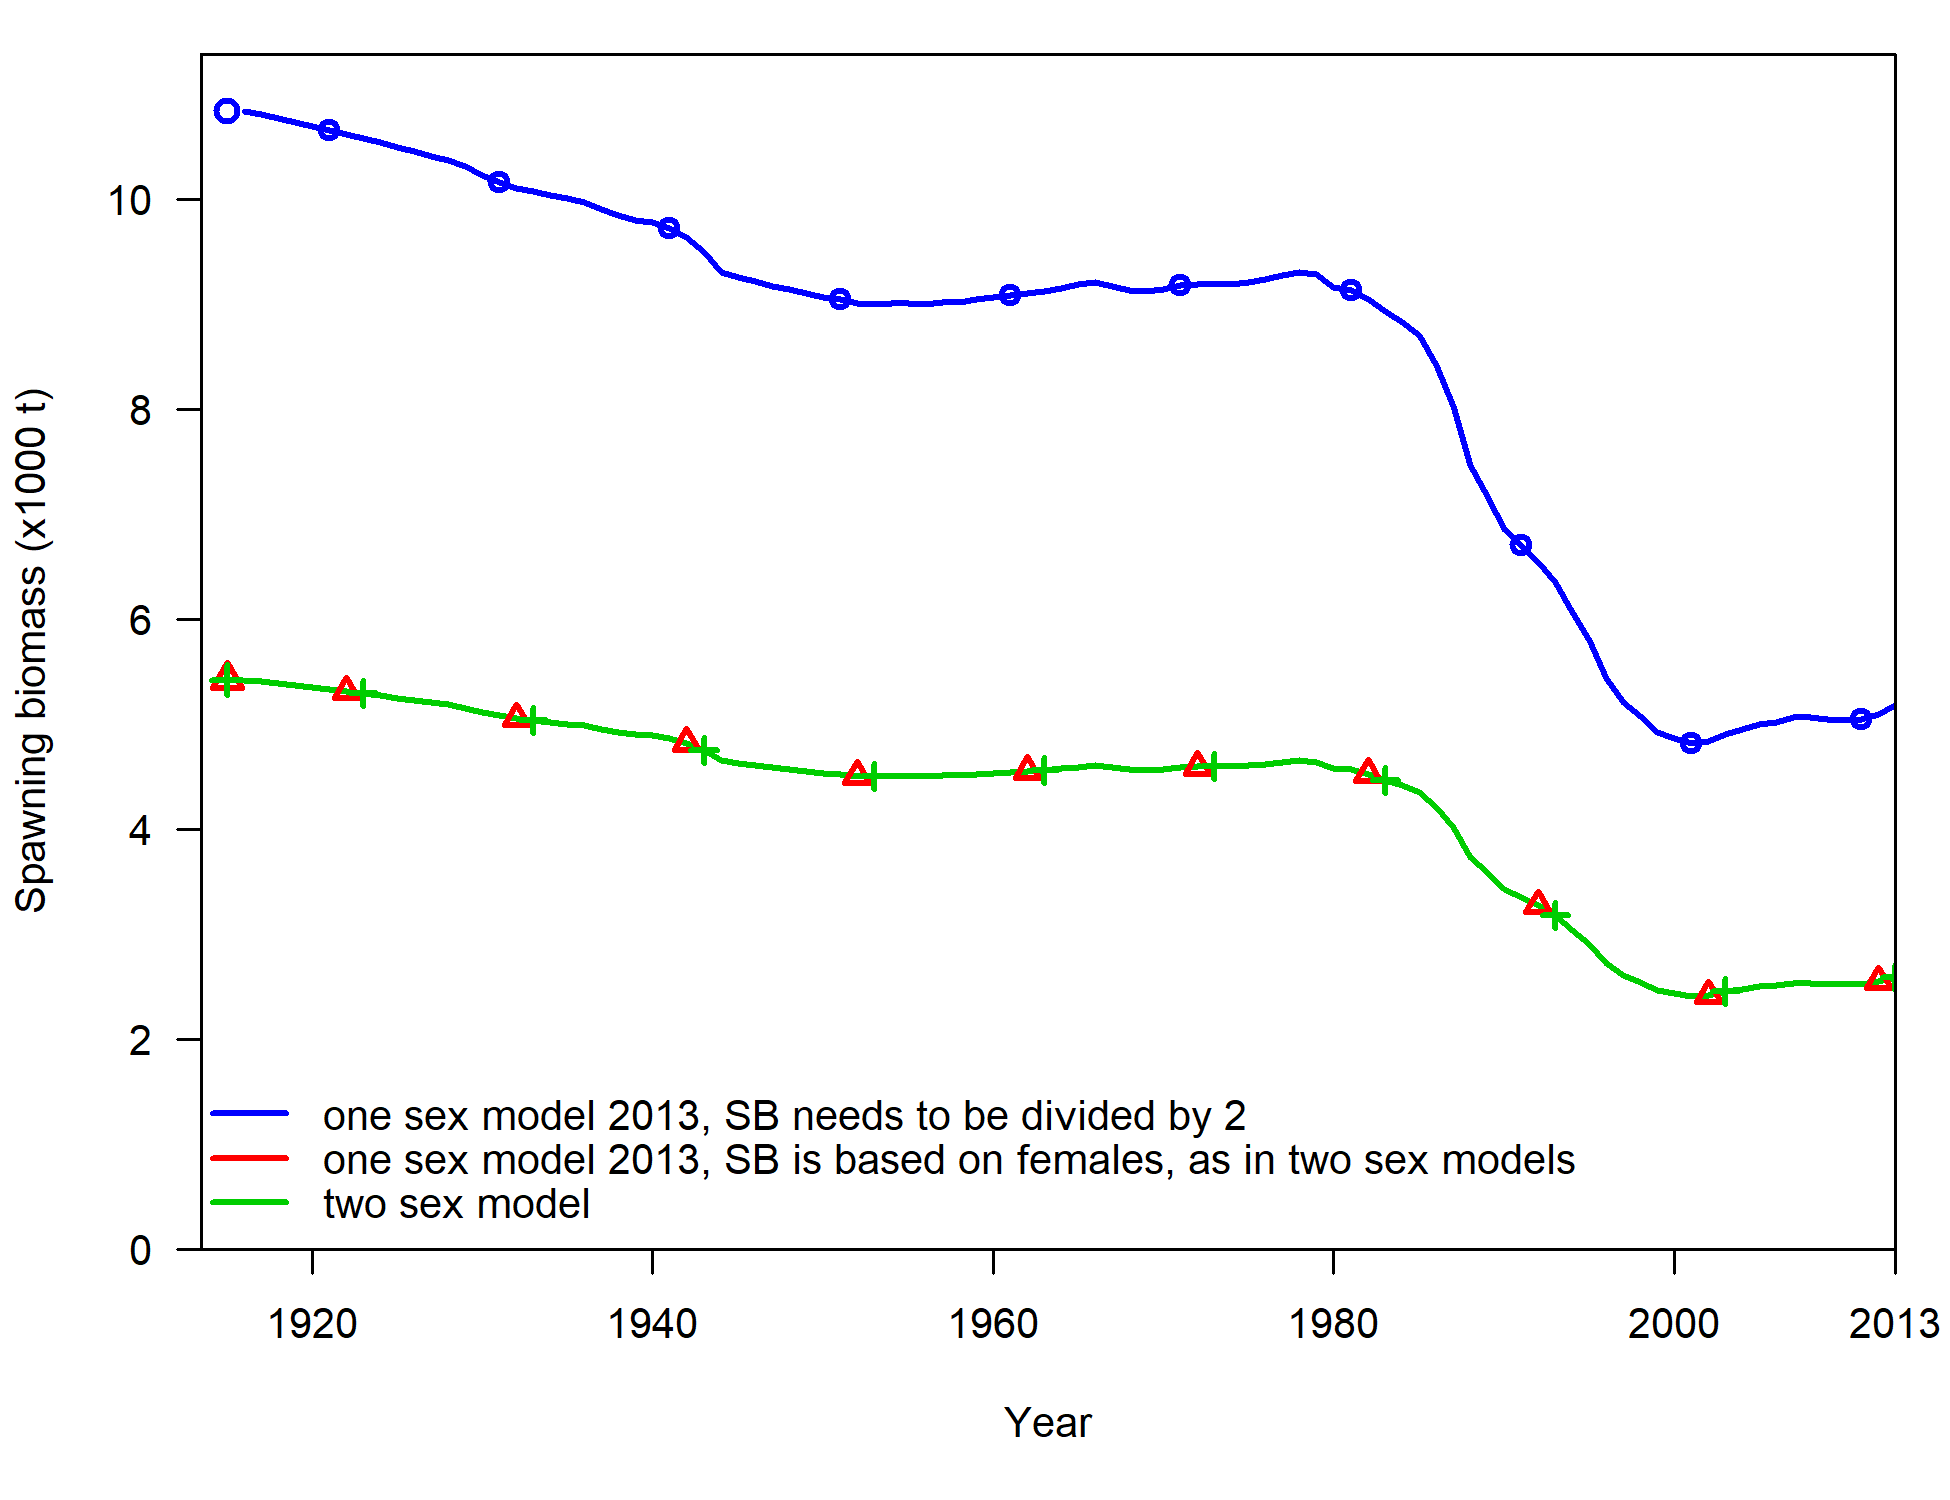
\includegraphics[keepaspectratio]{plots_4_doc/1v2sex_spawnbio.png}}

}

\caption{\label{fig-Sex1vs2_SO}Comparison of spawning output using the 1
sex and 2 sexes set to equal values models based on the 2013
Rougheye/Blackspotted Rockfishes assessment data. The 1 sex model has
double the biomass because it includes both females and males.}

\end{figure}%

\begin{figure}[H]

\centering{

\pandocbounded{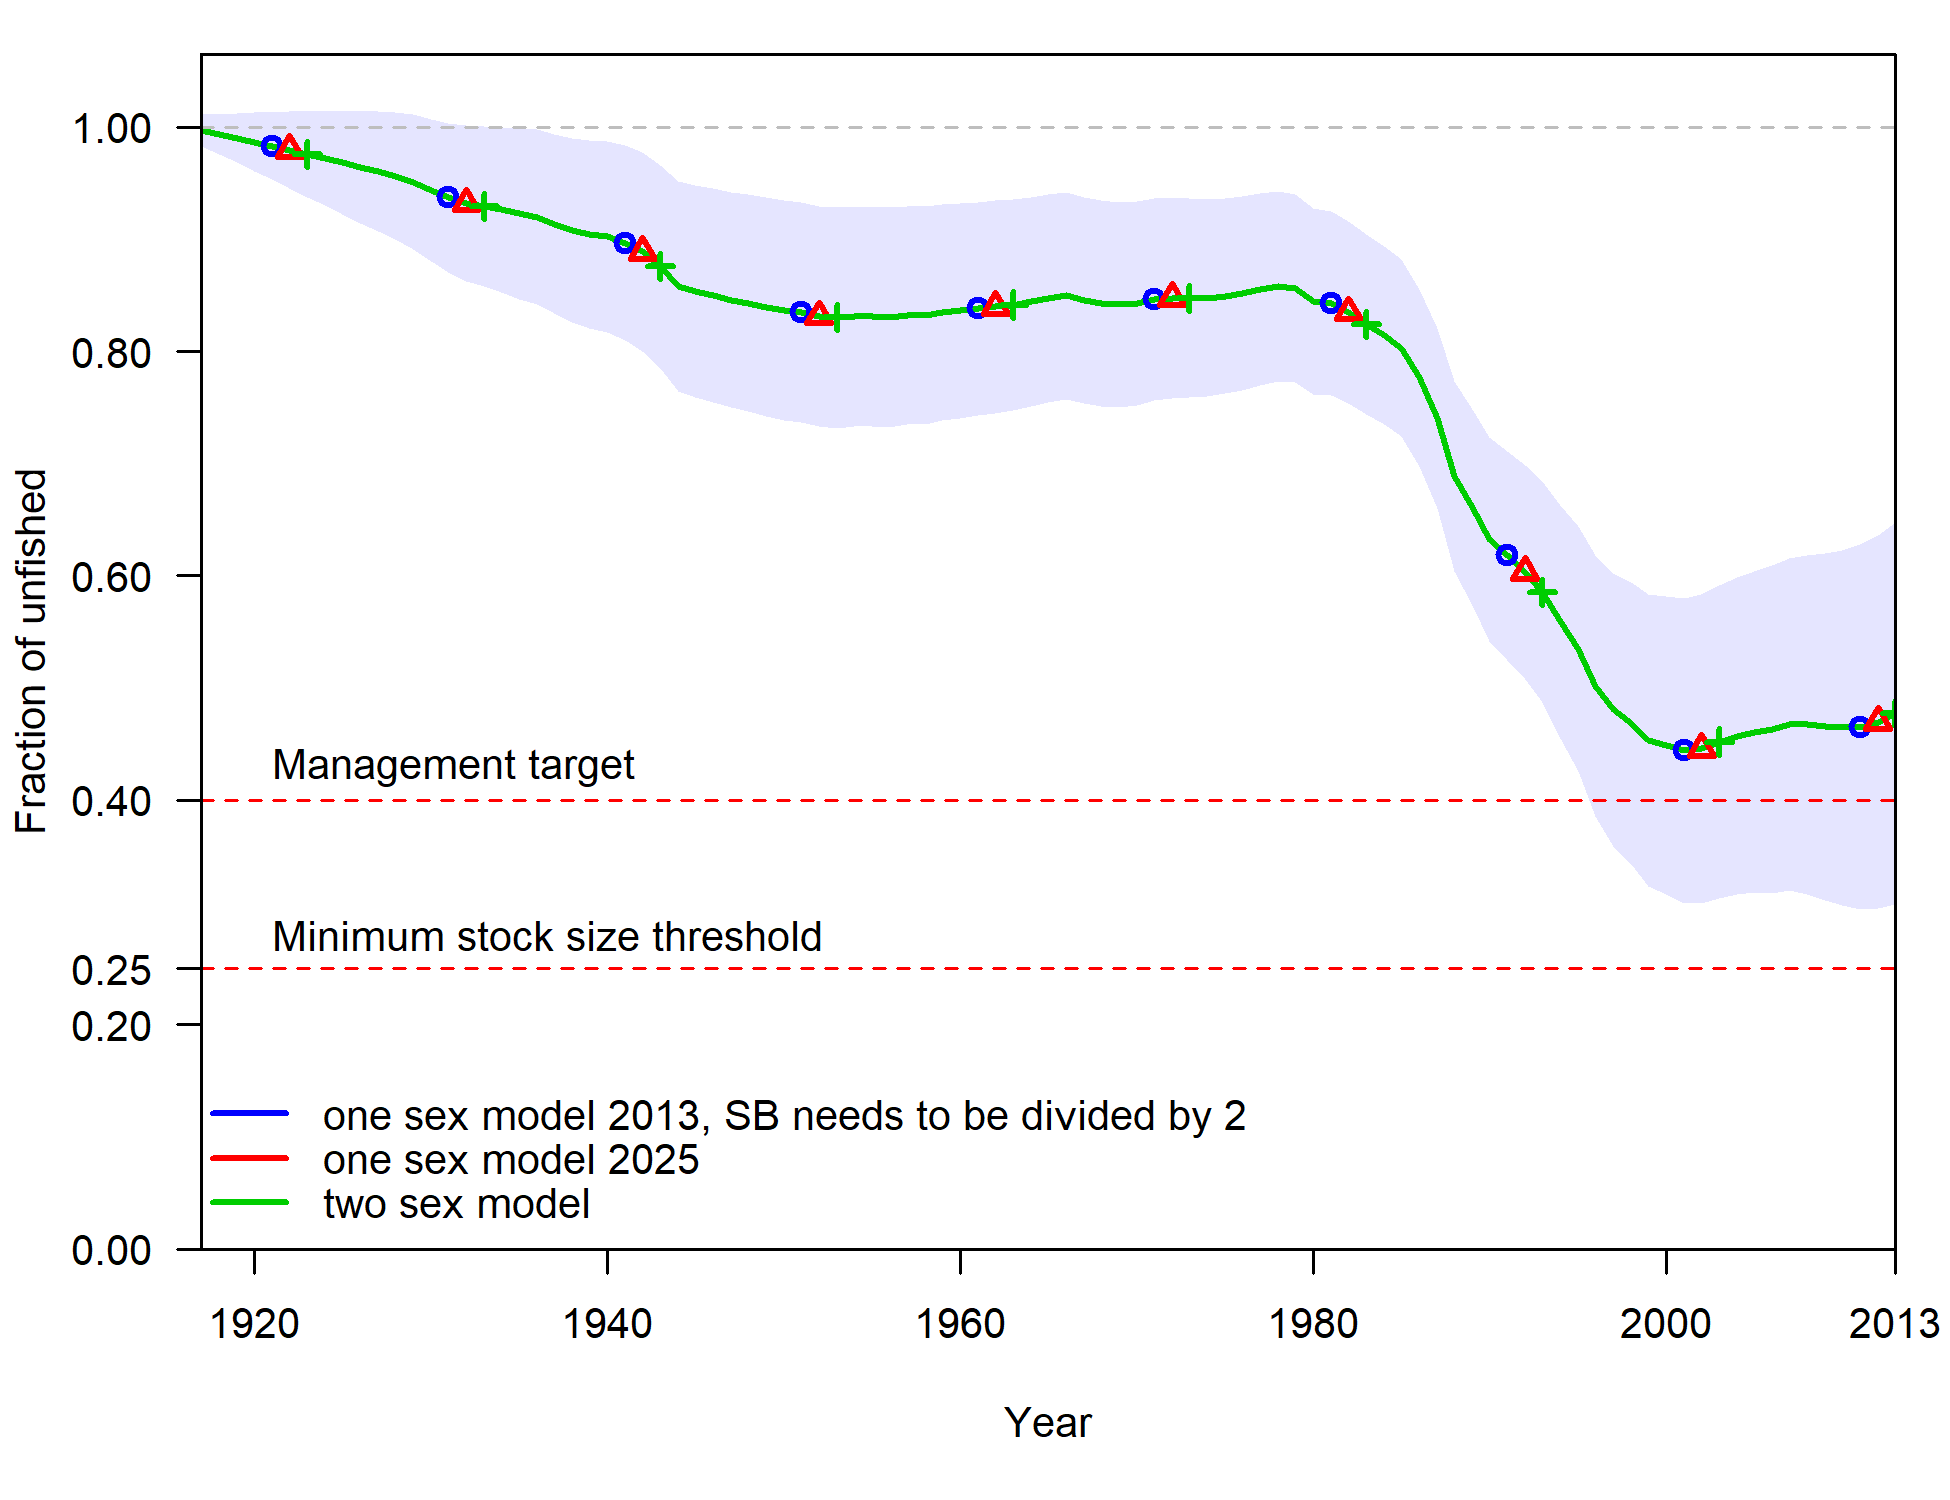
\includegraphics[keepaspectratio]{plots_4_doc/1v2sex_Bratio_uncertainty.png}}

}

\caption{\label{fig-Sex1vs2_Bratio}Comparison of spawning output using
the 1 sex and 2 sexes set to equal values models based on the 2013
Rougheye/Blackspotted Rockfishes assessment data.}

\end{figure}%

\begin{figure}[H]

\centering{

\pandocbounded{\includegraphics[keepaspectratio]{plots_4_doc/M_values.png}}

}

\caption{\label{fig-Mcurves}Natural mortality curves by age in years for
values of natural mortality used in various Rougheye/Blackspotted
Rockfish stock assessments. Dots indicate the range of assumed maximum
ages using the equation from Hamel and Cope 2022.}

\end{figure}%

\begin{figure}[H]

\centering{

\pandocbounded{\includegraphics[keepaspectratio]{plots_4_doc/Catch_curve_plot_FM.png}}

}

\caption{\label{fig-CC_Z}Catch curve (log abundance by age) analysis on
aggregated ages over all age sources by sex (black points). The peak
selected age was 21 for both sexes, so the linear model was run from age
21 until the oldest age (red points). The slope of the linear model is
equal to the estimate of an aggregate total mortality (Z).}

\end{figure}%

\begin{figure}[H]

\centering{

\pandocbounded{\includegraphics[keepaspectratio]{plots_4_doc/Catch_curve_plot_FM_21_100.png}}

}

\caption{\label{fig-CC_Z_100}Catch curve (log abundance by age) analysis
on aggregated ages over all age sources by sex (black points). The peak
selected age was 21 for both sexes with a max age of 100, so the linear
model was run from age 21 until age 100 (red points). The slope of the
linear model is equal to the estimate of an aggregate total mortality
(Z).}

\end{figure}%

\begin{figure}[H]

\centering{

\pandocbounded{\includegraphics[keepaspectratio]{plots_4_doc/Catch_curve_plot_FM_21_80.png}}

}

\caption{\label{fig-CC_Z_80}Catch curve (log abundance by age) analysis
on aggregated ages over all age sources by sex (black points). The peak
selected age was 21 for both sexes with a max age of 80, so the linear
model was run from age 21 until age 80 (red points). The slope of the
linear model is equal to the estimate of an aggregate total mortality
(Z).}

\end{figure}%

\begin{figure}[H]

\centering{

\pandocbounded{\includegraphics[keepaspectratio]{plots_4_doc/Age_length_plot.png}}

}

\caption{\label{fig-AL_1}Age and length data, with fitted von
Bertalanffy growth curves, by sex and data source for the
Rougheye/Blackspotted rockfish complex. Sample sizes (N) are also
provided.}

\end{figure}%

\begin{figure}[H]

\centering{

\pandocbounded{\includegraphics[keepaspectratio]{plots_4_doc/Lt_age_CV_FM.png}}

}

\caption{\label{fig-AL_2}Coefficient of variation by age and sex for all
sources of Rougheye/Blackspotted rockfishes ages. Sample sizes (N) are
also indicated by size of the point. The line is a smoothed loess
(polynomial) line that gives a moving average of CV by age and sex.}

\end{figure}%

\begin{figure}[H]

\centering{

\pandocbounded{\includegraphics[keepaspectratio]{plots_4_doc/AE_matrix_plot.png}}

}

\caption{\label{fig-AE_matrices}Ageing error matrix assignments by year
and data source. The number indicates which ageing error matrix was used
for conditional ages within those years and data sources. `Commercial'
is a combination of all commercial fleets.}

\end{figure}%

\begin{figure}[H]

\centering{

\pandocbounded{\includegraphics[keepaspectratio]{plots_4_doc/AE_Bias.png}}

}

\caption{\label{fig-AE_bias}Estimated bias used for each of the seven
ageing error matrices.}

\end{figure}%

\begin{figure}[H]

\centering{

\pandocbounded{\includegraphics[keepaspectratio]{plots_4_doc/AE_SD.png}}

}

\caption{\label{fig-AE_SD}Estimated imprecision (as a standard
deviation) used for each of the seven ageing error matrices.}

\end{figure}%

\newpage

\begin{figure}[H]

\centering{

\pandocbounded{\includegraphics[keepaspectratio]{plots_4_doc/L_W_plots.png}}

}

\caption{\label{fig-LW1}Length and weight samples by sex and data
source. Lines are the power function fits by data source.}

\end{figure}%

\begin{figure}[H]

\centering{

\pandocbounded{\includegraphics[keepaspectratio]{plots_4_doc/F_M_ltwt_plot.png}}

}

\caption{\label{fig-LW2}Realized length and weight relationships for
female and male Rougheye/Blackspotted Rockfishes.}

\end{figure}%

\newpage

\begin{figure}[H]

\centering{

\pandocbounded{\includegraphics[keepaspectratio]{plots_4_doc/bio_fxn_maturity.png}}

}

\caption{\label{fig-maturity_bio_fxn}Placeholder.}

\end{figure}%

\begin{figure}[H]

\centering{

\pandocbounded{\includegraphics[keepaspectratio]{plots_4_doc/l50_both_species.png}}

}

\caption{\label{fig-maturity_length_both}Placeholder.}

\end{figure}%

\begin{figure}[H]

\centering{

\pandocbounded{\includegraphics[keepaspectratio]{plots_4_doc/a50_both_species.png}}

}

\caption{\label{fig-maturity_age_both}Placeholder.}

\end{figure}%

\newpage

\begin{figure}[H]

\centering{

\pandocbounded{\includegraphics[keepaspectratio]{plots_4_doc/Bimodal_lengths_Peter_Frey.png}}

}

\caption{\label{fig-bimodal-lengths}Length distribution of Rougheye
Rockfish and Blackspotted Rockfish identified to species using genetics
(pers. comm. P. Prey, NWFSC).}

\end{figure}%

\begin{figure}[H]

\centering{

\pandocbounded{\includegraphics[keepaspectratio]{plots_4_doc/compare4_Bratio_uncertainty.png}}

}

\caption{\label{fig-RSS_2013}Estimates of relative stock size (current
spawning output/unfished spawning output) for the Rougheye/Blackspotted
rockfish complex in U.S. west coast waters from the 2013 assessment, and
compared to the using the same data in the newest version of SS3
(3.30.22.1).}

\end{figure}%

\begin{figure}[H]

\centering{

\pandocbounded{\includegraphics[keepaspectratio]{plots_4_doc/compare2_spawnbio_uncertainty.png}}

}

\caption{\label{fig-SO_2013}Estimates of spawning output for the
Rougheye/Blackspotted rockfish complex in U.S. west coast waters from
the 2013 assessment, and compared to the same data in the newest version
of SS3 (3.30.22.1). Shading denotes 95\% confidence intervals. Shading
denotes 95\% confidence intervals.}

\end{figure}%

\begin{figure}[H]

\centering{

\pandocbounded{\includegraphics[keepaspectratio]{plots_4_doc/compare1_spawnbio__discard_fleets.png}}

}

\caption{\label{fig-Discard_comp_SO}Comparison of spawning output using
retention curves or discard fleets using the 2013 Rougheye/Blackspotted
Rockfishes assessment.}

\end{figure}%

\begin{figure}[H]

\centering{

\pandocbounded{\includegraphics[keepaspectratio]{plots_4_doc/compare3_Bratio_discard_fleets.png}}

}

\caption{\label{fig-Discard_comp_RSS}Comparison of relative spawning
output using retention curves or discard fleets using the 2013
Rougheye/Blackspotted Rockfishes assessment.}

\end{figure}%

\begin{figure}[H]

\centering{

\pandocbounded{\includegraphics[keepaspectratio]{plots_4_doc/bridging_compare2_spawnbio_uncertainty.png}}

}

\caption{\label{fig-SO_Bridging}Time series of estimated spawning output
for briding analysis.}

\end{figure}%

\begin{figure}[H]

\centering{

\pandocbounded{\includegraphics[keepaspectratio]{plots_4_doc/bridging_compare4_Bratio_uncertainty.png}}

}

\caption{\label{fig-Bratio_Bridging}Time series of fraction of unfished
spawning output for briding analysis.}

\end{figure}%

\newpage

\begin{figure}[H]

\centering{

\pandocbounded{\includegraphics[keepaspectratio]{plots_4_doc/piner_panel_NatM_uniform_Mal_GP_1.png}}

}

\caption{\label{fig-M-profile-explore}Likelihood profile and component
likelihoods used to establish a fixed value for male natural mortality.}

\end{figure}%

\newpage

\begin{figure}[H]

\centering{

\pandocbounded{\includegraphics[keepaspectratio]{plots_4_doc/pairs_plot_fast.png}}

}

\caption{\label{fig-pairs_plot_fast}Pairs plots of the fastest mixing
parameters from running 2000 posterior draws (keeping every draw) using
the random walk Metropolis algorithm. Parameters that show little to no
movement are recommended to be fixed to improve model speed and
efficiency.}

\end{figure}%

\begin{figure}[H]

\centering{

\pandocbounded{\includegraphics[keepaspectratio]{ref_model/Jitter Results_0.01/jitterplot.png}}

}

\caption{\label{fig-jitter001}Jitter runs (using a value of 0.01) for
the reference model, with jitter run number on the x-axis and -log
likelihood value on the y-axis. Blue dot are models that match the
likelihood value of the reference model, while red dots deviate from the
reference model. All red dots are above the blue dots, indicating no
better fit to the reference model was found.}

\end{figure}%

\begin{figure}[H]

\centering{

\pandocbounded{\includegraphics[keepaspectratio]{ref_model/Jitter Results_0.05/jitterplot.png}}

}

\caption{\label{fig-jitter005}Jitter runs (using a value of 0.05) for
the reference model, with jitter run number on the x-axis and -log
likelihood value on the y-axis. Blue dot are models that match the
likelihood value of the reference model, while red dots deviate from the
reference model. All red dots are above the blue dots, indicating no
better fit to the reference model was found.}

\end{figure}%

\begin{figure}[H]

\centering{

\pandocbounded{\includegraphics[keepaspectratio]{ref_model/plots/comp_lenfit__aggregated_across_time.png}}

}

\caption{\label{fig-agg-len-fit}Aggregated length (cm) compositions over
all years.}

\end{figure}%

\begin{figure}[H]

\centering{

\pandocbounded{\includegraphics[keepaspectratio]{ref_model/plots/comp_lenfit_flt1mkt0_page1.png}}

}

\caption{\label{fig-len-fit-bt-1}Observed (gray density plot) and
expected (density lines by sex) length compositions by year for the
bottom trawl fishery in years available between 1995-2018.'N adj.' is
the input sample size after data-weighting adjustment. N eff. is the
calculated effective sample size used in the McAllister-Ianelli tuning
method.}

\end{figure}%

\begin{figure}[H]

\centering{

\pandocbounded{\includegraphics[keepaspectratio]{ref_model/plots/comp_lenfit_flt1mkt0_page2.png}}

}

\caption{\label{fig-len-fit-bt-2}Observed (gray density plot) and
expected (density lines by sex) length compositions by year for the
bottom trawl fishery in years available between 2019-2024.'N adj.' is
the input sample size after data-weighting adjustment. N eff. is the
calculated effective sample size used in the McAllister-Ianelli tuning
method.}

\end{figure}%

\begin{figure}[H]

\centering{

\pandocbounded{\includegraphics[keepaspectratio]{ref_model/plots/comp_lenfit_flt2mkt0.png}}

}

\caption{\label{fig-len-fit-btdis}Observed (gray density plot) and
expected (density lines) length compositions by year for the bottom
trawl discard fishery in years available between 2004-2023.'N adj.' is
the input sample size after data-weighting adjustment. N eff. is the
calculated effective sample size used in the McAllister-Ianelli tuning
method.}

\end{figure}%

\begin{figure}[H]

\centering{

\pandocbounded{\includegraphics[keepaspectratio]{ref_model/plots/comp_lenfit_flt3mkt0_page1.png}}

}

\caption{\label{fig-len-fit-nt-1}Observed (gray density plot) and
expected (density lines by sex) length compositions by year for the
non-trawl fishery in years available between 1996-2020.'N adj.' is the
input sample size after data-weighting adjustment. N eff. is the
calculated effective sample size used in the McAllister-Ianelli tuning
method.}

\end{figure}%

\begin{figure}[H]

\centering{

\pandocbounded{\includegraphics[keepaspectratio]{ref_model/plots/comp_lenfit_flt3mkt0_page2.png}}

}

\caption{\label{fig-len-fit-nt-2}Observed (gray density plot) and
expected (density lines by sex) length compositions by year for the
non-trawl fishery in years available between 2021-2024.'N adj.' is the
input sample size after data-weighting adjustment. N eff. is the
calculated effective sample size used in the McAllister-Ianelli tuning
method.}

\end{figure}%

\begin{figure}[H]

\centering{

\pandocbounded{\includegraphics[keepaspectratio]{ref_model/plots/comp_lenfit_flt4mkt0.png}}

}

\caption{\label{fig-len-fit-ntdis}Observed (gray density plot) and
expected (density lines) length compositions by year for the midwater
trawl fishery in years available between 2004-2024.'N adj.' is the input
sample size after data-weighting adjustment. N eff. is the calculated
effective sample size used in the McAllister-Ianelli tuning method.}

\end{figure}%

\begin{figure}[H]

\centering{

\pandocbounded{\includegraphics[keepaspectratio]{ref_model/plots/comp_lenfit_flt5mkt0.png}}

}

\caption{\label{fig-len-fit-midt}Observed (gray density plot) and
expected (density lines by sex) length compositions by year for the
non-trawl discard fishery in years available between 2000-2023.'N adj.'
is the input sample size after data-weighting adjustment. N eff. is the
calculated effective sample size used in the McAllister-Ianelli tuning
method.}

\end{figure}%

\begin{figure}[H]

\centering{

\pandocbounded{\includegraphics[keepaspectratio]{ref_model/plots/comp_lenfit_flt6mkt0.png}}

}

\caption{\label{fig-len-fit-ashop}Observed (gray density plot) and
expected (density lines by sex) length compositions by year for the
at-sea-hake fishery in years available between 2003-2024.'N adj.' is the
input sample size after data-weighting adjustment. N eff. is the
calculated effective sample size used in the McAllister-Ianelli tuning
method.}

\end{figure}%

\begin{figure}[H]

\centering{

\pandocbounded{\includegraphics[keepaspectratio]{ref_model/plots/comp_lenfit_flt7mkt0.png}}

}

\caption{\label{fig-len-fit-tri}Observed (gray density plot) and
expected (density lines by sex) length compositions by year for the
Triennial Bottom Trawl Survey in years available between 1980-2004.'N
adj.' is the input sample size after data-weighting adjustment. N eff.
is the calculated effective sample size used in the McAllister-Ianelli
tuning method.}

\end{figure}%

\begin{figure}[H]

\centering{

\pandocbounded{\includegraphics[keepaspectratio]{ref_model/plots/comp_lenfit_flt8mkt0.png}}

}

\caption{\label{fig-len-fit-akslope}Observed (gray density plot) and
expected (density lines by sex) length compositions by year for the
Alaskan Slope Bottom Trawl Survey in years available between
1997-2001.'N adj.' is the input sample size after data-weighting
adjustment. N eff. is the calculated effective sample size used in the
McAllister-Ianelli tuning method.}

\end{figure}%

\begin{figure}[H]

\centering{

\pandocbounded{\includegraphics[keepaspectratio]{ref_model/plots/comp_lenfit_flt10mkt0.png}}

}

\caption{\label{fig-len-fit-wcgbts}Observed (gray density plot) and
expected (density lines by sex) length compositions by year for the West
Coast Groundfish Bottom Trawl Survey in years available between
1980-2004.'N adj.' is the input sample size after data-weighting
adjustment. N eff. is the calculated effective sample size used in the
McAllister-Ianelli tuning method.}

\end{figure}%

\begin{figure}[H]

\centering{

\pandocbounded{\includegraphics[keepaspectratio]{ref_model/plots/comp_lenfit__page1_multi-fleet_comparison.png}}

}

\caption{\label{fig-peasrson-resids-fishery}Pearson residuals of length
fits for each fishing fleet. Closed bubble are positive residuals
(observed \textgreater{} expected) and open bubbles are negative
residuals (observed \textless{} expected).}

\end{figure}%

\begin{figure}[H]

\centering{

\pandocbounded{\includegraphics[keepaspectratio]{ref_model/plots/comp_lenfit__page2_multi-fleet_comparison.png}}

}

\caption{\label{fig-peasrson-resids-survey}Pearson residuals of length
fits for each survey. Closed bubble are positive residuals (observed
\textgreater{} expected) and open bubbles are negative residuals
(observed \textless{} expected).}

\end{figure}%

\begin{figure}[H]

\centering{

\pandocbounded{\includegraphics[keepaspectratio]{ref_model/plots/comp_lenfit_data_weighting_TA1-8_BOTTOM_TRAWL.png}}

}

\caption{\label{fig-meanlt-bt}Mean length (cm) index from the bottom
trawl fishery with 95 percent confidence intervals based on sample sizes
and data weighting.}

\end{figure}%

\begin{figure}[H]

\centering{

\pandocbounded{\includegraphics[keepaspectratio]{ref_model/plots/comp_lenfit_data_weighting_TA1-8_BOTTOM_TRAWL_DISCARD.png}}

}

\caption{\label{fig-meanlt-btdis}Mean length (cm) index from the bottom
trawl discard fishery with 95 percent confidence intervals based on
sample sizes and data weighting.}

\end{figure}%

\begin{figure}[H]

\centering{

\pandocbounded{\includegraphics[keepaspectratio]{ref_model/plots/comp_lenfit_data_weighting_TA1-8_NON_TRAWL.png}}

}

\caption{\label{fig-meanlt-nt}Mean length (cm) index from the non-trawl
fishery with 95 percent confidence intervals based on sample sizes and
data weighting.}

\end{figure}%

\begin{figure}[H]

\centering{

\pandocbounded{\includegraphics[keepaspectratio]{ref_model/plots/comp_lenfit_data_weighting_TA1-8_NON_TRAWL_DISCARD.png}}

}

\caption{\label{fig-meanlt-ntdis}Mean length (cm) index from the
non-trawl discard fishery with 95 percent confidence intervals based on
sample sizes and data weighting.}

\end{figure}%

\begin{figure}[H]

\centering{

\pandocbounded{\includegraphics[keepaspectratio]{ref_model/plots/comp_lenfit_data_weighting_TA1-8_MIDWATER_TRAWL.png}}

}

\caption{\label{fig-meanlt-midt}Mean length (cm) index from the midwater
trawl fishery with 95 percent confidence intervals based on sample sizes
and data weighting.}

\end{figure}%

\begin{figure}[H]

\centering{

\pandocbounded{\includegraphics[keepaspectratio]{ref_model/plots/comp_lenfit_data_weighting_TA1-8_AT_SEA_HAKE.png}}

}

\caption{\label{fig-meanlt-ashop}Mean length (cm) index from the
at-sea-hake fishery with 95 percent confidence intervals based on sample
sizes and data weighting.}

\end{figure}%

\begin{figure}[H]

\centering{

\pandocbounded{\includegraphics[keepaspectratio]{ref_model/plots/comp_lenfit_data_weighting_TA1-8_TRIENNIAL.png}}

}

\caption{\label{fig-meanlt-tri}Mean length (cm) index from the Triennial
survey with 95 percent confidence intervals based on sample sizes and
data weighting.}

\end{figure}%

\begin{figure}[H]

\centering{

\pandocbounded{\includegraphics[keepaspectratio]{ref_model/plots/comp_lenfit_data_weighting_TA1-8_AK_SLOPE.png}}

}

\caption{\label{fig-meanlt-akslope}Mean length (cm) index from the
Alaskan slope survey with 95 percent confidence intervals based on
sample sizes and data weighting.}

\end{figure}%

\begin{figure}[H]

\centering{

\pandocbounded{\includegraphics[keepaspectratio]{ref_model/plots/comp_lenfit_data_weighting_TA1-8_WCGBTS.png}}

}

\caption{\label{fig-meanlt-wcgbts}Mean length (cm) index from the West
Coast Groundfish Bottom Trawl survey with 95 percent confidence
intervals based on sample sizes and data weighting.}

\end{figure}%

\newpage

\begin{figure}[H]

\centering{

\pandocbounded{\includegraphics[keepaspectratio]{ref_model/plots/comp_condAALdat_bubflt1mkt0_page1.png}}

}

\caption{\label{fig-peasrson-resids-age-bt1}Pearson residuals of
conditional age at length fits for the bottom trawl fishery in the years
2008-2021. Closed bubble are positive residuals (observed \textgreater{}
expected) and open bubbles are negative residuals (observed \textless{}
expected).}

\end{figure}%

\begin{figure}[H]

\centering{

\pandocbounded{\includegraphics[keepaspectratio]{ref_model/plots/comp_condAALdat_bubflt1mkt0_page2.png}}

}

\caption{\label{fig-peasrson-resids-age-bt2}Pearson residuals of
conditional age at length fits for the bottom trawl fishery in the years
2022-2024. Closed bubble are positive residuals (observed \textgreater{}
expected) and open bubbles are negative residuals (observed \textless{}
expected).}

\end{figure}%

\begin{figure}[H]

\centering{

\pandocbounded{\includegraphics[keepaspectratio]{ref_model/plots/comp_condAALfit_residsflt3mkt0_page1.png}}

}

\caption{\label{fig-peasrson-resids-age-nt1}Pearson residuals of
conditional age at length fits for the non-trawl fishery in the years
2008-2021. Closed bubble are positive residuals (observed \textgreater{}
expected) and open bubbles are negative residuals (observed \textless{}
expected).}

\end{figure}%

\begin{figure}[H]

\centering{

\pandocbounded{\includegraphics[keepaspectratio]{ref_model/plots/comp_condAALfit_residsflt3mkt0_page2.png}}

}

\caption{\label{fig-peasrson-resids-age-nt2}Pearson residuals of
conditional age at length fits for the non-trawl fishery in the years
2022-2024. Closed bubble are positive residuals (observed \textgreater{}
expected) and open bubbles are negative residuals (observed \textless{}
expected).}

\end{figure}%

\begin{figure}[H]

\centering{

\pandocbounded{\includegraphics[keepaspectratio]{ref_model/plots/comp_condAALfit_residsflt5mkt0.png}}

}

\caption{\label{fig-peasrson-resids-age-midt}Pearson residuals of
conditional age at length fits for the midwater trawl fishery. Closed
bubble are positive residuals (observed \textgreater{} expected) and
open bubbles are negative residuals (observed \textless{} expected).}

\end{figure}%

\begin{figure}[H]

\centering{

\pandocbounded{\includegraphics[keepaspectratio]{ref_model/plots/comp_condAALfit_residsflt6mkt0_page1.png}}

}

\caption{\label{fig-peasrson-resids-age-ashop1}Pearson residuals of
conditional age at length fits for the at-sea-hake fishery in the years
2008-2022. Closed bubble are positive residuals (observed \textgreater{}
expected) and open bubbles are negative residuals (observed \textless{}
expected).}

\end{figure}%

\begin{figure}[H]

\centering{

\pandocbounded{\includegraphics[keepaspectratio]{ref_model/plots/comp_condAALfit_residsflt6mkt0_page2.png}}

}

\caption{\label{fig-peasrson-resids-age-ashop2}Pearson residuals of
conditional age at length fits for the at-sea-hake fishery in the years
2023-2024. Closed bubble are positive residuals (observed \textgreater{}
expected) and open bubbles are negative residuals (observed \textless{}
expected).}

\end{figure}%

\begin{figure}[H]

\centering{

\pandocbounded{\includegraphics[keepaspectratio]{ref_model/plots/comp_condAALfit_residsflt10mkt0_page1.png}}

}

\caption{\label{fig-peasrson-resids-age-wcgbts1}Pearson residuals of
conditional age at length fits for the West Coast Groundfish Bottom
Trawl survey in the years 2003-2010. Closed bubble are positive
residuals (observed \textgreater{} expected) and open bubbles are
negative residuals (observed \textless{} expected).}

\end{figure}%

\begin{figure}[H]

\centering{

\pandocbounded{\includegraphics[keepaspectratio]{ref_model/plots/comp_condAALfit_residsflt10mkt0_page2.png}}

}

\caption{\label{fig-peasrson-resids-age-wcgbts2}Pearson residuals of
conditional age at length fits for the West Coast Groundfish Bottom
Trawl survey in the years 2011-2018. Closed bubble are positive
residuals (observed \textgreater{} expected) and open bubbles are
negative residuals (observed \textless{} expected).}

\end{figure}%

\begin{figure}[H]

\centering{

\pandocbounded{\includegraphics[keepaspectratio]{ref_model/plots/comp_condAALfit_residsflt10mkt0_page3.png}}

}

\caption{\label{fig-peasrson-resids-age-wcgbts3}Pearson residuals of
conditional age at length fits for the West Coast Groundfish Bottom
Trawl survey in the years 2019-2024. Closed bubble are positive
residuals (observed \textgreater{} expected) and open bubbles are
negative residuals (observed \textless{} expected).}

\end{figure}%

\begin{figure}[H]

\centering{

\pandocbounded{\includegraphics[keepaspectratio]{ref_model/plots/comp_condAALfit_data_weighting_TA1-8_condAgeBOTTOM_TRAWL.png}}

}

\caption{\label{fig-trawl-mean-caal}Mean age from conditional
age-at-length data for the trawl fishery with 95\% confidence intervals
based on current samples sizes and data weighting.}

\end{figure}%

\begin{figure}[H]

\centering{

\pandocbounded{\includegraphics[keepaspectratio]{ref_model/plots/comp_condAALfit_data_weighting_TA1-8_condAgeNON_TRAWL.png}}

}

\caption{\label{fig-nontrawl-mean-caal}Mean age from conditional
age-at-length data for the non-trawl fishery with 95\% confidence
intervals based on current samples sizes and data weighting.}

\end{figure}%

\begin{figure}[H]

\centering{

\pandocbounded{\includegraphics[keepaspectratio]{ref_model/plots/comp_condAALfit_data_weighting_TA1-8_condAgeMIDWATER_TRAWL.png}}

}

\caption{\label{fig-midwater-mean-caal}Mean age from conditional
age-at-length data for the midwater trawl fishery with 95\% confidence
intervals based on current samples sizes and data weighting.}

\end{figure}%

\begin{figure}[H]

\centering{

\pandocbounded{\includegraphics[keepaspectratio]{ref_model/plots/comp_condAALfit_data_weighting_TA1-8_condAgeAT_SEA_HAKE.png}}

}

\caption{\label{fig-ashop-mean-caal}Mean age from conditional
age-at-length data for the at-sea-hake fishery with 95\% confidence
intervals based on current samples sizes and data weighting.}

\end{figure}%

\begin{figure}[H]

\centering{

\pandocbounded{\includegraphics[keepaspectratio]{ref_model/plots/comp_condAALfit_data_weighting_TA1-8_condAgeWCGBTS.png}}

}

\caption{\label{fig-wcgbts-mean-caal}Mean age from conditional
age-at-length data for the West Coast Groundfish Bottom Trawl survey
with 95\% confidence intervals based on current samples sizes and data
weighting.}

\end{figure}%

\begin{figure}[H]

\centering{

\pandocbounded{\includegraphics[keepaspectratio]{ref_model/plots/comp_condAALfit_Andre_plotsflt1mkt0_page1.png}}

}

\caption{\label{fig-call-plot-bt1}Conditional age at length plot showing
mean age (left panels) and standard deviation (right panels) for the
bottom trawl fishery in years 2008-2011. The CIs are 90\% based on
adding 1.64 SE of mean to the data for the left panels and the standard
error of mean age at length (obs. and exp.) with 90\% CIs based on the
chi-square distribution.}

\end{figure}%

\begin{figure}[H]

\centering{

\pandocbounded{\includegraphics[keepaspectratio]{ref_model/plots/comp_condAALfit_Andre_plotsflt1mkt0_page2.png}}

}

\caption{\label{fig-call-plot-bt2}Conditional age at length plot showing
mean age (left panels) and standard deviation (right panels) for the
bottom trawl fishery in years 2012-2021. The CIs are 90\% based on
adding 1.64 SE of mean to the data for the left panels and the standard
error of mean age at length (obs. and exp.) with 90\% CIs based on the
chi-square distribution.}

\end{figure}%

\begin{figure}[H]

\centering{

\pandocbounded{\includegraphics[keepaspectratio]{ref_model/plots/comp_condAALfit_Andre_plotsflt1mkt0_page3.png}}

}

\caption{\label{fig-call-plot-bt3}Conditional age at length plot showing
mean age (left panels) and standard deviation (right panels) for the
bottom trawl fishery in years 2022-2024. The CIs are 90\% based on
adding 1.64 SE of mean to the data for the left panels and the standard
error of mean age at length (obs. and exp.) with 90\% CIs based on the
chi-square distribution.}

\end{figure}%

\begin{figure}[H]

\centering{

\pandocbounded{\includegraphics[keepaspectratio]{ref_model/plots/comp_condAALfit_Andre_plotsflt3mkt0_page1.png}}

}

\caption{\label{fig-call-plot-nt1}Conditional age at length plot showing
mean age (left panels) and standard deviation (right panels) for the
non-trawl fishery in years 2008-2011. The CIs are 90\% based on adding
1.64 SE of mean to the data for the left panels and the standard error
of mean age at length (obs. and exp.) with 90\% CIs based on the
chi-square distribution.}

\end{figure}%

\begin{figure}[H]

\centering{

\pandocbounded{\includegraphics[keepaspectratio]{ref_model/plots/comp_condAALfit_Andre_plotsflt3mkt0_page2.png}}

}

\caption{\label{fig-call-plot-nt2}Conditional age at length plot showing
mean age (left panels) and standard deviation (right panels) for the
non-trawl fishery in years 2012-2021. The CIs are 90\% based on adding
1.64 SE of mean to the data for the left panels and the standard error
of mean age at length (obs. and exp.) with 90\% CIs based on the
chi-square distribution.}

\end{figure}%

\begin{figure}[H]

\centering{

\pandocbounded{\includegraphics[keepaspectratio]{ref_model/plots/comp_condAALfit_Andre_plotsflt3mkt0_page3.png}}

}

\caption{\label{fig-call-plot-nt3}Conditional age at length plot showing
mean age (left panels) and standard deviation (right panels) for the
non-trawl fishery in years 2022-2024. The CIs are 90\% based on adding
1.64 SE of mean to the data for the left panels and the standard error
of mean age at length (obs. and exp.) with 90\% CIs based on the
chi-square distribution.}

\end{figure}%

\begin{figure}[H]

\centering{

\pandocbounded{\includegraphics[keepaspectratio]{ref_model/plots/comp_condAALfit_Andre_plotsflt5mkt0_page1.png}}

}

\caption{\label{fig-call-plot-midt1}Conditional age at length plot
showing mean age (left panels) and standard deviation (right panels) for
the midwater trawl fishery in years 2011-2022. The CIs are 90\% based on
adding 1.64 SE of mean to the data for the left panels and the standard
error of mean age at length (obs. and exp.) with 90\% CIs based on the
chi-square distribution.}

\end{figure}%

\begin{figure}[H]

\centering{

\pandocbounded{\includegraphics[keepaspectratio]{ref_model/plots/comp_condAALfit_Andre_plotsflt5mkt0_page2.png}}

}

\caption{\label{fig-call-plot-midt2}Conditional age at length plot
showing mean age (left panels) and standard deviation (right panels) for
the non-trawl fishery in years 2023-2024. The CIs are 90\% based on
adding 1.64 SE of mean to the data for the left panels and the standard
error of mean age at length (obs. and exp.) with 90\% CIs based on the
chi-square distribution.}

\end{figure}%

\begin{figure}[H]

\centering{

\pandocbounded{\includegraphics[keepaspectratio]{ref_model/plots/comp_condAALfit_Andre_plotsflt6mkt0_page1.png}}

}

\caption{\label{fig-call-plot-ashop1}Conditional age at length plot
showing mean age (left panels) and standard deviation (right panels) for
the at-sea-hake fishery in years 2008-2016. The CIs are 90\% based on
adding 1.64 SE of mean to the data for the left panels and the standard
error of mean age at length (obs. and exp.) with 90\% CIs based on the
chi-square distribution.}

\end{figure}%

\begin{figure}[H]

\centering{

\pandocbounded{\includegraphics[keepaspectratio]{ref_model/plots/comp_condAALfit_Andre_plotsflt6mkt0_page2.png}}

}

\caption{\label{fig-call-plot-ashop2}Conditional age at length plot
showing mean age (left panels) and standard deviation (right panels) for
the at-sea-hake fishery in years 2019-2022. The CIs are 90\% based on
adding 1.64 SE of mean to the data for the left panels and the standard
error of mean age at length (obs. and exp.) with 90\% CIs based on the
chi-square distribution.}

\end{figure}%

\begin{figure}[H]

\centering{

\pandocbounded{\includegraphics[keepaspectratio]{ref_model/plots/comp_condAALfit_Andre_plotsflt6mkt0_page3.png}}

}

\caption{\label{fig-call-plot-ashop3}Conditional age at length plot
showing mean age (left panels) and standard deviation (right panels) for
the at-sea-hake fishery in years 2023-2024. The CIs are 90\% based on
adding 1.64 SE of mean to the data for the left panels and the standard
error of mean age at length (obs. and exp.) with 90\% CIs based on the
chi-square distribution.}

\end{figure}%

\begin{figure}[H]

\centering{

\pandocbounded{\includegraphics[keepaspectratio]{ref_model/plots/comp_condAALfit_Andre_plotsflt10mkt0_page1.png}}

}

\caption{\label{fig-call-plot-wcgbts1}Conditional age at length plot
showing mean age (left panels) and standard deviation (right panels) for
the West Coast Groundfish Bottom Trawl survey in years 2003-2006. The
CIs are 90\% based on adding 1.64 SE of mean to the data for the left
panels and the standard error of mean age at length (obs. and exp.) with
90\% CIs based on the chi-square distribution.}

\end{figure}%

\begin{figure}[H]

\centering{

\pandocbounded{\includegraphics[keepaspectratio]{ref_model/plots/comp_condAALfit_Andre_plotsflt10mkt0_page2.png}}

}

\caption{\label{fig-call-plot-wcgbts2}Conditional age at length plot
showing mean age (left panels) and standard deviation (right panels) for
the West Coast Groundfish Bottom Trawl survey in years 2007-2010. The
CIs are 90\% based on adding 1.64 SE of mean to the data for the left
panels and the standard error of mean age at length (obs. and exp.) with
90\% CIs based on the chi-square distribution.}

\end{figure}%

\begin{figure}[H]

\centering{

\pandocbounded{\includegraphics[keepaspectratio]{ref_model/plots/comp_condAALfit_Andre_plotsflt10mkt0_page3.png}}

}

\caption{\label{fig-call-plot-wcgbts3}Conditional age at length plot
showing mean age (left panels) and standard deviation (right panels) for
the West Coast Groundfish Bottom Trawl survey in years 2011-2014. The
CIs are 90\% based on adding 1.64 SE of mean to the data for the left
panels and the standard error of mean age at length (obs. and exp.) with
90\% CIs based on the chi-square distribution.}

\end{figure}%

\begin{figure}[H]

\centering{

\pandocbounded{\includegraphics[keepaspectratio]{ref_model/plots/comp_condAALfit_Andre_plotsflt10mkt0_page4.png}}

}

\caption{\label{fig-call-plot-wcgbts4}Conditional age at length plot
showing mean age (left panels) and standard deviation (right panels) for
the West Coast Groundfish Bottom Trawl survey in years 2015-2018. The
CIs are 90\% based on adding 1.64 SE of mean to the data for the left
panels and the standard error of mean age at length (obs. and exp.) with
90\% CIs based on the chi-square distribution.}

\end{figure}%

\begin{figure}[H]

\centering{

\pandocbounded{\includegraphics[keepaspectratio]{ref_model/plots/comp_condAALfit_Andre_plotsflt10mkt0_page5.png}}

}

\caption{\label{fig-call-plot-wcgbts5}Conditional age at length plot
showing mean age (left panels) and standard deviation (right panels) for
the West Coast Groundfish Bottom Trawl survey in years 2019-2023. The
CIs are 90\% based on adding 1.64 SE of mean to the data for the left
panels and the standard error of mean age at length (obs. and exp.) with
90\% CIs based on the chi-square distribution.}

\end{figure}%

\begin{figure}[H]

\centering{

\pandocbounded{\includegraphics[keepaspectratio]{ref_model/plots/comp_condAALfit_Andre_plotsflt10mkt0_page6.png}}

}

\caption{\label{fig-call-plot-wcgbts6}Conditional age at length plot
showing mean age (left panels) and standard deviation (right panels) for
the West Coast Groundfish Bottom Trawl survey in 2024. The CIs are 90\%
based on adding 1.64 SE of mean to the data for the left panels and the
standard error of mean age at length (obs. and exp.) with 90\% CIs based
on the chi-square distribution.}

\end{figure}%

\begin{figure}[H]

\centering{

\pandocbounded{\includegraphics[keepaspectratio]{ref_model/plots/comp_gstagefit_flt1mkt0.png}}

}

\caption{\label{fig-marage_bt}Realized fits (lines) to the marginal age
composition data (density) for the bottom trawl fishery.}

\end{figure}%

\begin{figure}[H]

\centering{

\pandocbounded{\includegraphics[keepaspectratio]{ref_model/plots/comp_gstagefit_flt3mkt0.png}}

}

\caption{\label{fig-marage_nt}Realized fits (lines) to the marginal age
composition data (density) for the non-trawl fishery.}

\end{figure}%

\begin{figure}[H]

\centering{

\pandocbounded{\includegraphics[keepaspectratio]{ref_model/plots/comp_gstagefit_flt5mkt0.png}}

}

\caption{\label{fig-marage_midt}Realized fits (lines) to the marginal
age composition data (density) for the midwater trawl fishery.}

\end{figure}%

\begin{figure}[H]

\centering{

\pandocbounded{\includegraphics[keepaspectratio]{ref_model/plots/comp_gstagefit_flt6mkt0.png}}

}

\caption{\label{fig-marage_ashop}Realized fits (lines) to the marginal
age composition data (density) for the at-sea-hake fishery.}

\end{figure}%

\begin{figure}[H]

\centering{

\pandocbounded{\includegraphics[keepaspectratio]{ref_model/plots/comp_gstagefit_flt10mkt0.png}}

}

\caption{\label{fig-marage_wcgbts}Realized fits (lines) to the marginal
age composition data (density) for the West Coast Groundfish Bottom
Trawl survey.}

\end{figure}%

\begin{figure}[H]

\centering{

\pandocbounded{\includegraphics[keepaspectratio]{ref_model/plots/index2_cpuefit_TRIENNIAL.png}}

}

\caption{\label{fig-index-tri}Fit to index data for Triennial survey.
Lines indicate 95\% uncertainty interval around index values based on
the assumption of lognormal error.}

\end{figure}%

\begin{figure}[H]

\centering{

\pandocbounded{\includegraphics[keepaspectratio]{ref_model/plots/index2_cpuefit_AK_SLOPE.png}}

}

\caption{\label{fig-index-akslope}Fit to index data for the Alaska Slope
survey. Lines indicate 95\% uncertainty interval around index values
based on the assumption of lognormal error.}

\end{figure}%

\begin{figure}[H]

\centering{

\pandocbounded{\includegraphics[keepaspectratio]{ref_model/plots/index2_cpuefit_NW_SLOPE.png}}

}

\caption{\label{fig-index-nwslope}Fit to index data for Northwest
Fisheries Science Center Slope survey. Lines indicate 95\% uncertainty
interval around index values based on the assumption of lognormal
error.}

\end{figure}%

\begin{figure}[H]

\centering{

\pandocbounded{\includegraphics[keepaspectratio]{ref_model/plots/index2_cpuefit_WCGBTS.png}}

}

\caption{\label{fig-index-wcgbts}Fit to index data for West Coast
Groundfish Bottom Trawl survey. Lines indicate 95\% uncertainty interval
around index values based on the assumption of lognormal error.}

\end{figure}%

\begin{figure}[H]

\centering{

\pandocbounded{\includegraphics[keepaspectratio]{ref_model/plots/bio1_sizeatage.png}}

}

\caption{\label{fig-vbgf}Estimated age and growth relatioship in the
reference model .Shaded area indicates 95\% distribution of length at
age around estimated growth curve.}

\end{figure}%

\begin{figure}[H]

\centering{

\pandocbounded{\includegraphics[keepaspectratio]{ref_model/plots/sel01_multiple_fleets_length1.png}}

}

\caption{\label{fig-sel-all}Ending selectivity at length for each
fishery and survey.}

\end{figure}%

\begin{figure}[H]

\centering{

\pandocbounded{\includegraphics[keepaspectratio]{plots_4_doc/selectivityPlot_fisheries.png}}

}

\caption{\label{fig-sel-tv-fisheries}Time-varying selectivity for
fishery fleets with time blocks.}

\end{figure}%

\begin{figure}[H]

\centering{

\pandocbounded{\includegraphics[keepaspectratio]{plots_4_doc/selectivityPlot_surveys.png}}

}

\caption{\label{fig-sel-tv-surveys}Time-varying selectivity for surveys
with time blocks.}

\end{figure}%

\begin{figure}[H]

\centering{

\pandocbounded{\includegraphics[keepaspectratio]{ref_model/plots/sel02_multiple_fleets_age2.png}}

}

\caption{\label{fig-sel-all-age}Ending selectivity at age derived from
lengths for each fishery and survey.}

\end{figure}%

\begin{figure}[H]

\centering{

\pandocbounded{\includegraphics[keepaspectratio]{plots_4_doc/lnR0.png}}

}

\caption{\label{fig-lnR0}Estimated unfished recruitment (lnR0) for
several assessed shelf and slope rockfishes.}

\end{figure}%

\begin{figure}[H]

\centering{

\pandocbounded{\includegraphics[keepaspectratio]{ref_model/plots/ts7_Spawning_output_with_95_intervals.png}}

}

\caption{\label{fig-spawnout}Estimated time series of spawning output
(in millions of eggs) for the reference model.}

\end{figure}%

\begin{figure}[H]

\centering{

\pandocbounded{\includegraphics[keepaspectratio]{ref_model/plots/ts9_Relative_spawning_output_intervals.png}}

}

\caption{\label{fig-depl}Estimated time series of fraction of unfished
spawning output for the reference model.}

\end{figure}%

\begin{figure}[H]

\centering{

\pandocbounded{\includegraphics[keepaspectratio]{ref_model/plots/recdevs2_withbars.png}}

}

\caption{\label{fig-recdevs}Estimated time series of recruitment
deviations for the base model.}

\end{figure}%

\begin{figure}[H]

\centering{

\pandocbounded{\includegraphics[keepaspectratio]{ref_model/plots/recruit_fit_bias_adjust.png}}

}

\caption{\label{fig-biasramp}Bias adjustment applied to the recruitment
deviations (red line). Points are transformed variances relative to the
assumed variance of recruitment.}

\end{figure}%

\begin{figure}[H]

\centering{

\pandocbounded{\includegraphics[keepaspectratio]{ref_model/plots/ts11_Age-0_recruits_(1000s)_with_95_asymptotic_intervals.png}}

}

\caption{\label{fig-recruits}Estimated time series of age-0 recruits for
the base model.}

\end{figure}%

\begin{figure}[H]

\centering{

\pandocbounded{\includegraphics[keepaspectratio]{ref_model/plots/SR_curve2.png}}

}

\caption{\label{fig-SR}Stock-recruit curve with labels on first, last,
and years with (log) deviations \textgreater{} 0.5. Point colors
indicate year, with warmer colors indicating earlier years and cooler
colors in showing later years.}

\end{figure}%

\pagebreak

\begin{figure}[H]

\centering{

\pandocbounded{\includegraphics[keepaspectratio]{Retros/compare2_spawnbio_uncertainty.png}}

}

\caption{\label{fig-retro-so}Change in the estimate of spawning output
(millions of eggs) when the five most recent years of data area removed
sequentially.}

\end{figure}%

\begin{figure}[H]

\centering{

\pandocbounded{\includegraphics[keepaspectratio]{Retros/compare4_Bratio_uncertainty.png}}

}

\caption{\label{fig-retro-status}Change in the estimate of relative
stock status when the five most recent years of data area removed
sequentially.}

\end{figure}%

\newpage

\begin{figure}[H]

\centering{

\pandocbounded{\includegraphics[keepaspectratio]{Sensis/output/indicescompare2_spawnbio_uncertainty.png}}

}

\caption{\label{fig-sens_indices_spout}Spawning output (millions of
eggs) across data removal sensitivities (indices).}

\end{figure}%

\begin{figure}[H]

\centering{

\pandocbounded{\includegraphics[keepaspectratio]{Sensis/output/indicescompare4_Bratio_uncertainty.png}}

}

\caption{\label{fig-sens_indices_relsp}Relative spawning output
(fraction unfished) across data removal sensitivities (indices).}

\end{figure}%

\begin{figure}[H]

\centering{

\pandocbounded{\includegraphics[keepaspectratio]{Sensis/output/length_comps_fleetcompare2_spawnbio_uncertainty.png}}

}

\caption{\label{fig-sens_lens1_spout}Spawning output (millions of eggs)
across data removal sensitivities (length compositions by fleet).}

\end{figure}%

\begin{figure}[H]

\centering{

\pandocbounded{\includegraphics[keepaspectratio]{Sensis/output/length_comps_fleetcompare4_Bratio_uncertainty.png}}

}

\caption{\label{fig-sens_lens1_relsp}Relative spawning output (fraction
unfished) across data removal sensitivities (length compositions by
fleet).}

\end{figure}%

\begin{figure}[H]

\centering{

\pandocbounded{\includegraphics[keepaspectratio]{Sensis/output/length_comps_allcompare2_spawnbio_uncertainty.png}}

}

\caption{\label{fig-sens_lens2_spout}Spawning output (millions of eggs)
across data removal sensitivities (length compositions by source).}

\end{figure}%

\begin{figure}[H]

\centering{

\pandocbounded{\includegraphics[keepaspectratio]{Sensis/output/length_comps_allcompare4_Bratio_uncertainty.png}}

}

\caption{\label{fig-sens_lens2_relsp}Relative spawning output (fraction
unfished) across data removal sensitivities (length compositions by
source).}

\end{figure}%

\begin{figure}[H]

\centering{

\pandocbounded{\includegraphics[keepaspectratio]{Sensis/output/age_compscompare2_spawnbio_uncertainty.png}}

}

\caption{\label{fig-sens_age_spout}Spawning output (millions of eggs)
across data removal sensitivities (age compositions by fleet).}

\end{figure}%

\begin{figure}[H]

\centering{

\pandocbounded{\includegraphics[keepaspectratio]{Sensis/output/age_compscompare4_Bratio_uncertainty.png}}

}

\caption{\label{fig-sens_age_relsp}Relative spawning output (fraction
unfished) across data removal sensitivities (age compositions by
fleet).}

\end{figure}%

\begin{figure}[H]

\centering{

\pandocbounded{\includegraphics[keepaspectratio]{Sensis/output/sens_summary.png}}

}

\caption{\label{fig-sens_sum_data}Relative change in management
quantities across models conducted as sensitivities (removal of data
sources).}

\end{figure}%

\begin{figure}[H]

\centering{

\pandocbounded{\includegraphics[keepaspectratio]{Sensis/data_sensitivities/Data weighting.png}}

}

\caption{\label{fig-sensi-data-wt}Comparison of spawning output (left
panel), relative stock status (middle panel) and recruitment estimation
(right panel) for models under different data weighting scenarios. The
reference model uses the Francis method.}

\end{figure}%

\begin{figure}[H]

\centering{

\pandocbounded{\includegraphics[keepaspectratio]{Sensis/data_sensitivities/Sensi_logREplot_SB_Dep_F_Yield_DataWt.png}}

}

\caption{\label{fig-sensi-RE-data-wt}Log relative change
(log((Model\_sensi-Model\_ref)/Model\_ref)) in data weighting treatment
for 5 derived quantities. Colored boxes indicate 95 percent confidence
interval of the reference model. See `Sensitivity Analysis' section for
more details on each scenario.}

\end{figure}%

\begin{figure}[H]

\centering{

\pandocbounded{\includegraphics[keepaspectratio]{Sensis/data_sensitivities/Ageing error_uncertainty.png}}

}

\caption{\label{fig-sensi-ageing-error}Comparison of spawning output
(left panel), relative stock status (middle panel) and recruitment
estimation (right panel) for models under different ageing error
scenarios. The reference model uses ageing error matrices for all age
sources.}

\end{figure}%

\begin{figure}[H]

\centering{

\pandocbounded{\includegraphics[keepaspectratio]{Sensis/data_sensitivities/Sensi_logREplot_SB_Dep_F_Yield_AE.png}}

}

\caption{\label{fig-sensi-RE-ageing-error}Log relative change
(log((Model\_sensi-Model\_ref)/Model\_ref)) in ageing error scenarios
for 5 derived quantities. Colored boxes indicate 95 percent confidence
interval of the reference model. See `Sensitivity Analysis' section for
more details on each scenario.}

\end{figure}%

\begin{figure}[H]

\centering{

\pandocbounded{\includegraphics[keepaspectratio]{Sensis/model_specs/M_Gr_Reproduction.png}}

}

\caption{\label{fig-sensi-LH}Comparison of spawning output (left panel),
relative stock status (middle panel) and recruitment estimation (right
panel) for models under different natural mortality, growth and
reproductive biology scenarios.}

\end{figure}%

\begin{figure}[H]

\centering{

\pandocbounded{\includegraphics[keepaspectratio]{Sensis/model_specs/Sensi_logREplot_SB_Dep_F_Yield_MGrRep.png}}

}

\caption{\label{fig-sensi-RE-LH}Log relative change
(log((Model\_sensi-Model\_ref)/Model\_ref)) in natural mortality, growth
and reproductive biology scenarios for 5 derived quantities. Colored
boxes indicate 95 percent confidence interval of the reference model.
See `Sensitivity Analysis' section for more details on each scenario.}

\end{figure}%

\begin{figure}[H]

\centering{

\pandocbounded{\includegraphics[keepaspectratio]{Sensis/model_specs/compare1_spawnbio_MGrRepro.png}}

}

\caption{\label{fig-sensi-LH-so}Comparison of spawning output for models
under different natural mortality, growth and reproductive biology
scenarios. This comparison excludes the model estimating natural
mortality, as the scale goes extremely high.}

\end{figure}%

\begin{figure}[H]

\centering{

\pandocbounded{\includegraphics[keepaspectratio]{Sensis/model_specs/Sel_Rec.png}}

}

\caption{\label{fig-sensi-SelRec}Comparison of spawning output (left
panel), relative stock status (middle panel) and recruitment estimation
(right panel) for models under different recruitment and selectivity
scenarios.}

\end{figure}%

\begin{figure}[H]

\centering{

\pandocbounded{\includegraphics[keepaspectratio]{Sensis/model_specs/Sensi_logREplot_SB_Dep_F_Yield_Sel_Rec.png}}

}

\caption{\label{fig-sensi-RE-SelRec}Log relative change
(log((Model\_sensi-Model\_ref)/Model\_ref)) in recruitment and
selectivity scenarios for 5 derived quantities. Colored boxes indicate
95 percent confidence interval of the reference model. See `Sensitivity
Analysis' section for more details on each scenario.}

\end{figure}%

\begin{figure}[H]

\centering{

\pandocbounded{\includegraphics[keepaspectratio]{Sensis/model_specs/comp_lenfit__aggregated_across_time_logsel.png}}

}

\caption{\label{fig-sensi-logsel_fits}Aggregate fit to length
compositions for the scenario that assume logistic selectivity for all
fisheries and time blocks.}

\end{figure}%

\newpage

\begin{figure}[H]

\centering{

\pandocbounded{\includegraphics[keepaspectratio]{Like_profiles/lnR0/parameter_panel_SR_LN(R0).png}}

}

\caption{\label{fig-likeprof-lnR0-parm}Initial recruitment (\(lnR_0\))
likelihood profile (change in the negative log-likelihood across a range
of \(ln(R0)\) values) and derived quantities. Red line in the top left
figure indicates the significance level in likelihood difference.}

\end{figure}%

\begin{figure}[H]

\centering{

\pandocbounded{\includegraphics[keepaspectratio]{Like_profiles/lnR0/piner_panel_SR_LN(R0).png}}

}

\caption{\label{fig-likeprof-lnR0-components}Initial recruitment
(\(ln(R0)\)) likelihood profile for each of the likelihood components.}

\end{figure}%

\begin{figure}[H]

\centering{

\pandocbounded{\includegraphics[keepaspectratio]{Like_profiles/Steepness/parameter_panel_SR_BH_steep.png}}

}

\caption{\label{fig-likeprof-h-parm}Steepness (\(h\)) likelihood profile
(change in the negative log-likelihood across a range of \(h\) values)
and derived quantities. Red line in the top left figure indicates the
significance level in likelihood difference.}

\end{figure}%

\begin{figure}[H]

\centering{

\pandocbounded{\includegraphics[keepaspectratio]{Like_profiles/Steepness/piner_panel_SR_BH_steep.png}}

}

\caption{\label{fig-likeprof-h-components}Steepness (\(h\)) likelihood
profile for each of the likelihood components.}

\end{figure}%

\begin{figure}[H]

\centering{

\pandocbounded{\includegraphics[keepaspectratio]{Like_profiles/Male_M/parameter_panel_NatM_uniform_Mal_GP_1.png}}

}

\caption{\label{fig-likeprof-M-parm}Male natural mortality (\(M\))
likelihood profile (change in the negative log-likelihood across a range
of male \(M\) values) and derived quantities. Red line in the top left
figure indicates the significance level in likelihood difference.}

\end{figure}%

\begin{figure}[H]

\centering{

\pandocbounded{\includegraphics[keepaspectratio]{Like_profiles/Male_M/M_sex.png}}

}

\caption{\label{fig-likeprof-M-sex}Likelihood differences by natural
mortality (\(M\)) by sex.}

\end{figure}%

\begin{figure}[H]

\centering{

\pandocbounded{\includegraphics[keepaspectratio]{Like_profiles/Male_M/piner_panel_NatM_uniform_Mal_GP_1.png}}

}

\caption{\label{fig-likeprof-M-components}Male natural mortality (\(M\))
likelihood profile for each of the likelihood components.}

\end{figure}%

\begin{figure}[H]

\centering{

\pandocbounded{\includegraphics[keepaspectratio]{Sensis/statesofnature/StatesofNature.png}}

}

\caption{\label{fig-states-of-nature}Comparison of spawning output (left
panel), relative stock status (middle panel) and recruitment estimation
(right panel) for the reference model and high and low states of
nature.}

\end{figure}%

\begin{figure}[H]

\centering{

\pandocbounded{\includegraphics[keepaspectratio]{Sensis/statesofnature/Ensemble_Bratio.png}}

}

\caption{\label{fig-ensemble}Ensemble relative stock status for the
reference model and two states of nature.}

\end{figure}%

\newpage

\newpage

\begin{figure}[H]

\centering{

\pandocbounded{\includegraphics[keepaspectratio]{ref_model/plots/ts9_Relative_spawning_output_intervals.png}}

}

\caption{\label{fig-management-depletion}Placeholder.}

\end{figure}%

\begin{figure}[H]

\centering{

\pandocbounded{\includegraphics[keepaspectratio]{ref_model/plots/SPR3_ratiointerval.png}}

}

\caption{\label{fig-one-minus-spr}Placeholder.}

\end{figure}%

\begin{figure}[H]

\centering{

\pandocbounded{\includegraphics[keepaspectratio]{ref_model/plots/yield2_yield_curve_with_refpoints.png}}

}

\caption{\label{fig-management-yield}Placeholder.}

\end{figure}%

\begin{figure}[H]

\centering{

\pandocbounded{\includegraphics[keepaspectratio]{ref_model/plots/SPR4_phase.png}}

}

\caption{\label{fig-management-phase}Placeholder.}

\end{figure}%

\begin{figure}[H]

\centering{

\pandocbounded{\includegraphics[keepaspectratio]{ref_model/plots/SPR3_ratiointerval.png}}

}

\caption{\label{fig-spr}Estimated time series of fishing intensity for
the base model.}

\end{figure}%

\begin{figure}[H]

\centering{

\pandocbounded{\includegraphics[keepaspectratio]{ref_model/plots/ts_DynamicB0.png}}

}

\caption{\label{fig-dyn-b0}Dynamic B0 plot. The lower line shows the
time series of estimated spawning output in the presence of fishing
mortality. The upper line shows the time series that could occur under
the same dynamics (including deviations in recruitment), but without
fishing. The point at the left represents the unfished equilibrium.}

\end{figure}%

\newpage{}

\section{Notes}\label{notes}

\newpage{}

\section{Appendices}\label{sec-appendix}




\end{document}
